\makeatletter
   \def\input@path{{..}} % 搜索上层目录的 LALUbook
\makeatother

\documentclass[
    % colors = false,
    geometry = 16k,
]{LALUbook}

\usepackage{booktabs} % Excel 导出的大表格
\usepackage{rotating}
\usepackage{extarrows}

\usepackage{float}
\usepackage{diagbox}
\usepackage{caption}

\usepackage{pgfplots}
\usetikzlibrary{cd, arrows, arrows.meta, calc, intersections, decorations.pathreplacing, patterns, decorations.markings}
\pgfplotsset{compat=newest}

\usepackage[xindy, splitindex]{imakeidx}
\makeindex[
    columns=1,
    program=truexindy,
    intoc=true,
    options=-M texindy -I xelatex -C utf8,
    title={名词索引}
] % 名词索引
\makeindex[
    columns=3,
    program=truexindy,
    intoc=true,
    options=-M numeric-sort -M latex -M latex-loc-fmts -M makeindex -I xelatex -C utf8,
    name=sym,
    title={符号索引}
] % 符号索引

% 嵌套 enumerate 环境的 label
\setlist[enumerate,2]{label=(\arabic*)}
\setlist[enumerate,3]{label=\roman*.}

\usepackage{xparse}
\NewDocumentCommand{\term}{m}{{\sffamily\heiti\bfseries{#1}}}

% 标题格式
% \chapter   正常专题
% \LUchapter 未竟专题

\newcounter{LUchapter}
\newcounter{LUgreekchap}

\makeatletter
% 此处可按需增改
% \texorpdfstring 的两个参数分别显示在正文中与 PDF 书签中
% 已知 bug:未竟专题中的定理等环境不可有标题(见 FIXME)
\newcommand*{\@LUgreek}[1]{%
    \ifcase#1\or\texorpdfstring{$\boldsymbol{\varepsilon}$}{ε}%
    \or\texorpdfstring{$\boldsymbol{\delta}$}{δ}%
    \or\texorpdfstring{$\boldsymbol{\lambda}$}{λ}%
    \or\texorpdfstring{$\boldsymbol{\mu}$}{μ}%
    \or\texorpdfstring{$\boldsymbol{\varphi}$}{φ}%
    \or\texorpdfstring{$\boldsymbol{\theta}$}{θ}%
    \else\@ctrerr\fi%
}
\newcommand*{\LUgreek}[1]{%
    \expandafter\@LUgreek\csname c@#1\endcsname
}
\newcommand*{\LUchapsancheck}{%
\expandafter\@ifundefined{@exist@LUchapter@\arabic{chapter}.\arabic{LUgreekchap}}%
    {\setcounter{LUgreekchap}{1}}
    {\stepcounter{LUgreekchap}}
}
\newcommand*{\LUgroupsancheck}{%
\expandafter\@ifundefined{@exist@LUchapter@\arabic{chapter}}%
    {}
    {\endgroup}
}
\let\@std@chapter\chapter
\renewcommand*{\chapter}{%
    \LUgroupsancheck%
    \@std@chapter
}
\makeatother

\NewDocumentCommand{\LUchapter}{m}{%
\LUgroupsancheck
\begingroup
\LUchapsancheck
\addtocounter{chapter}{-1}
\refstepcounter{LUchapter}
\renewcommand*{\thechapter}{\arabic{chapter}\LUgreek{LUgreekchap}}
\renewcommand*{\theHchapter}{LU.\arabic{LUchapter}}
\ctexset{
    chapter = {format={\centering\Huge\bfseries},name={未竟专题,},number={\zhnumber{\arabic{LUchapter}}}},
    section = {format={\raggedright\Large\bfseries},name={,},number={\thechapter.\arabic{section}}},
    subsection = {format={\raggedright\large\bfseries},name={,},number={\thesection.\arabic{subsection}}},
    subsubsection = {format={\raggedright\normalsize\bfseries},name={,},number={\thesubsection.\arabic{subsubsection}}},
}
\csname @std@chapter\endcsname{#1}
\expandafter\xdef\csname @exist@LUchapter@\arabic{chapter}\endcsname{\relax}
\expandafter\xdef\csname @exist@LUchapter@\arabic{chapter}.\arabic{LUgreekchap}\endcsname{\relax}
}

\ctexset{
    chapter = {format={\centering\Huge\bfseries},name={第,讲},number=\arabic{chapter}},
    section = {format={\raggedright\Large\bfseries},name={,},number={\arabic{chapter}.\arabic{section}}},
    subsection = {format={\raggedright\large\bfseries},name={,},number={\arabic{chapter}.\arabic{section}.\arabic{subsection}}},
    subsubsection = {format={\raggedright\normalsize\bfseries},name={,},number={\arabic{chapter}.\arabic{section}.\arabic{subsection}.\arabic{subsubsection}}},
}

\title{\heiti 浙江大学 2023--2024 学年 \\ 线性代数荣誉课辅学讲义}
\author{2023--2024 学年线性代数 I/II(H)辅学授课 \\ 吴一航 \quad \verb|yhwu_is@zju.edu.cn|}

\AtEndPreamble{\hypersetup{
    hypertexnames = true,
    pdfauthor = {吴一航},
    pdftitle = {线性代数荣誉课辅学讲义},
}}

\begin{document}
\frontmatter

% 封面,代替 \maketitle
\includepdf[
    pages={1},
    noautoscale=true,
    trim=0 0 0 10mm,
    clip,
]{./figs/cover-16k.pdf}

\songti

% 插入空页
\thispagestyle{empty}
\null
\clearpage

\thispagestyle{empty}
\thispagestyle{empty}
\vspace*{\fill}
\begin{center}
    \Large 致每一个阳光下闪烁着七彩光芒的泡沫

    \vspace{2ex}

    \large \textit{To every bubble glittering with colorful lights under the sun}
\end{center}
\vspace*{\fill}

\clearpage

\setcounter{page}{1}
\chapter*{序}

\section*{一些初衷}

我为这本讲义起了一个大胆的标题,它来源于浙江大学竺可桢学院线性代数II(H)课程选用的教材《线性代数应该这样学》(英文原版名:《Linear Algebra Done Right》)。我们带着半娱乐性质地将最后两个单词像矩阵求逆一样(见封面设计)进行了颠倒,得到了本书的英文名:《Linear Algebra Left Undone》。

接下来我们遇到了一个问题:中文名应该是什么呢?郑俊达同学提供了一个可行解:《线性代数:未竟之美》。转念一想,这一标题不能更契合我们的编写初衷。事实上,我们认为现行的大部分线性代数或高等代数教材具有如下问题,它们也困扰了笔者和许多读者的学习,我们也给出了解决的方案:
\begin{enumerate}
    \item 从线性代数的角度来看,它们的讲解顺序不够自然,大部分教材都从行列式起步,缺乏引入地给出各种概念,使得读者无法理解线性代数的本质。可以说这些教材应当更名``行列式与矩阵计算'',因为线性代数着重研究的线性空间和线性映射反而成为了边缘内容。因此我们采取了更好的讲解思路,更能体现线性代数的美感而非延续高中填鸭式的数学教育——事实上那根本称不上数学,那样的讲授思路根本不够``数学'',失去了数学本身的自然之美,而且使得读者误解数学、厌恶数学;

    \item 浙江大学竺可桢学院两学期线性代数课程选择的《大学数学:代数与几何》和《线性代数应该这样学》教材采用了从抽象空间引入的方式,更贴近本质。但实践过程中许多同学会对``为什么要一开始就学习这些抽象内容''缺乏概念,特别是《线性代数应该这样学》对于工科同学而言``数学味道太浓'',因此最后可能学习效果还不如填鸭式地灌输解题方法。因此我们在讲义中相当于为教材做了很多的注脚,并且优化了整体设计,提供了大量例题习题,都是为了能更自然地引入抽象内容,让读者知道我们为何要学习这些内容,这些内容当年在数学家眼中最自然的状态是什么,这样才能使得抽象的概念易于被初学者接受;

    \item 我们的例题和习题编排也是精心设计过的,不会出现大部分教材使用过程中``上课讲的、作业做的和考试考的脱节''的情况,这一问题不只是很多数学基础课教学的问题,也是国内各个专业都存在的教学问题,笔者也深受其害,所以编写例题习题特别注重对概念和定理的理解、对方法的掌握,不会出现教材中说什么知识很重要但没有例子体会很重要的这种抽象情况,并且大量的习题贴近所学知识也贴近考试,让读者通过习题更好地掌握知识而非反而迷惑不知道自己学了什么,才能更好地体会线性代数的美感而非感受到题海的压迫;

    \item 除了自然的美感外,更重要的是还有``未竟''的美感。线性代数是一个古老而年轻的学科。它发轫于早先对线性方程组的研究,经历了漫长的几何和代数的交错作用,最后又在近世代数的发展过程中被严格化。直到现在,一些相关的内容,例如线性代数群的研究尚且方兴未艾,在现代数学的种种支线当中也有着重要的应用。另外,它的方法论,尤其是其对代数结构的研究在现代数学中也具备着代表性。因此,我们希望呈现一个更广阔的线性代数观,从线性代数出发,对它的现代发展和它在现代数学的各个分支的应用进行一些导论性的介绍,这一方面是为了使得平淡的叙述更加有趣,另一方面也是为了回答一个疑问:线性代数到底有什么用?我们相信,这是许多初学者都有的一个问题,回答这个问题既需要对线性代数的深入学习,也需要有一个现代数学的全局观,这也就带来了本书的另一个部分,未竟专题,也是我们这本书的标题来源。
\end{enumerate}

古人有三不朽:立德、立功、立言,著书立说即为立言。虽说我完全不可能因为编写了一本基础课的讲义而有如此崇高的地位。但在我心里,我已经通过这本讲义将我的热情、我的想法传达给了不少的读者,这样也无愧于我在浙江大学的本科四年。未来或许这本讲义会淹没在历史的风尘中,但我想只要它的某行文字曾经给予读者一丝丝的启发,或更实际地帮助了读者得到了心仪的分数,我想它就是有价值的,我本人的价值也得到了一定的实现。

\section*{本书的面世}

自2021年秋参与浙江大学竺可桢学院学研部(现竺可桢学院学业指导中心)组织的朋辈辅学活动以来,我即将第三次参与线性代数荣誉课的辅学活动。犹记讲义最初的简陋版本,那时为了辅学的期中、期末准备的简单复习提要,里面因为本人时间有限甚至缺少了特征值与特征向量的内容。那时的讲义基本都是知识点的罗列,缺少了许多重要的例题和证明,犹记第一次拿起这个讲义站上讲台的时候,我深刻体会到了这一讲义的不足,因此那次的授课整体而言较为玄学,比较干瘪。因此在2022年再次参加辅学授课时,我借着疫情放开考试延迟的机会分了六个大专题写出了一本相对完整的适合于《大学数学:代数与几何》的复习讲义。里面的讲解比较全面,习题也十分丰富,可以说在复习资料中已经能算过得去的一版了。

但我并不满足于此,我希望这本讲义能成为一本真正的完整的讲义,能兼具配套学习、考试复习的功能,并且在保证体系严谨完整的前提下有更优化的讲解逻辑。因此在2023年的暑假,我基于原先的复习版本进行扩展重排。在这一版本中,我将原先复习资料中的粗略描述都换为了严谨的完整叙述,并且反复打磨讲解顺序,从而更自然地将另一本教材《线性代数应该这样学》的内容自然融合,并且添加了大量的remark更适合于初学者学习。更重要的是,我们中间添加了许多文字叙述,一方面自然引入我们要讲解的内容,这对于初学者而言是很重要的insight,另一方面反复强调我们的行文逻辑,对推进逻辑做适当总结,使得读者能更快地形成体系,同时也补充了很多拓展内容,一些是为了方便读者更自然地理解抽象内容,有一些是契合``未竟之美''的标题,让读者能体会到数学的美感,体会到学习线性代数后我们知识的边界可以推广到多远。

\section*{致谢}

我或许首先需要感谢2022年疫情放开之下的寒冬,没有这学期线性代数考试的延期,我也不会有如此充裕的时间整理出本讲义较为完整的底稿,也就没有这一完整讲义的面世。

在编写的过程中,我需要特别感谢下面记为同学对我的讲义提供了直接的支持:梅敏炫同学主编了讲义内积部分,郑俊达同学主编了解析几何部分,周健均同学编写了行列式计算进阶部分,朱熙哲和谢集同学负责了讲义习题答案部分。特别感谢李英琦同学全权负责了本讲义的格式设计以及插图,感谢王鹤翔同学设计了本讲义的封面。

我还需要感谢同级的王和钧同学,感谢他当年push我写出了最初版本的复习提要。我要感谢比我低一级的郭苗苗同学,感谢她当年反复邀请我走上讲台实现梦想,虽然可能第一次授课效果一般,但这对于后来我不断打磨授课方式,打磨讲义有非常重要的意义。我也应当感谢竺可桢学院学研部(现竺可桢学院学业指导中心)给我提供了一个辅学的平台,让我通过讲义将我的热情能传达给更多的读者。我还需要感谢支持我前面版本,对前面版本无论赞扬或是提出意见的读者们,正是有了大家的支持才有了接下来越来越好的版本的面世。

我想我也应该特别感谢数学科学学院的吴志祥、谈之奕和刘康生老师,他们在我线性代数入门过程中做了重要的引路人的工作,讲义中许多讲解思路也来源于他们精彩的授课。我也应该特别感谢数学科学学院的王晓光老师,他在复变函数课程以及讲义上的热情以及倾注的心血启发我也应该将我的学习思路和经验通过讲义传达给更多人,并且启发我思考如何从更高的观点、更自然的角度引导读者学习新知识,享受追求真理的过程。

\section*{参考文献}

本讲义作为浙江大学竺可桢学院线性代数荣誉课的辅学讲义,因此核心思路来源于我们选择的教材《大学数学:代数与几何(第二版)》(居余马,李海中)、《大学数学:代数与几何学习辅导》(林翠琴,居余马)、《线性代数应该这样学(第三版)》([美]Sheldon Axler)。

在编写与修订的过程中,我也参考了其他非常多优质的教材或辅导资料,如《高等代数(第二版)》(丘维声)、《高等代数:学习指导书》(丘维声)、《高等代数学(第四版)》(谢启鸿,姚慕生,吴泉水)、《高等代数学(第四版)配套学习用书》(谢启鸿,姚慕生)、《线性代数辅导讲义》(汤家凤)、《高等代数强化讲义》(李扬)以及《高等代数考研:高频真题分类精解300例》等,在复数域的引入部分我也简单参考了王晓光老师的《复变函数讲义(2023版)》,在矩阵计算等专题则部分参考了《数值分析》(Timothy Sauer)、《矩阵分析》(Roger A.Horn,Charles R.Johnson)等计算数学著作。

最后如果读者学完本讲义后对代数学有浓厚的兴趣,非常推荐读者学习后续的抽象代数课程。这里推荐与我同级的图灵班同学编写的\href{https://frightenedfoxcn.github.io/notes/series/alg-for-cs/}{《写给计算机系学生的代数》}作进一步的了解,我们许多高级专题都对这一讲义有引用。

\begin{flushright}
    \kaishu
    吴一航 \\
    浙江大学计算机科学与技术学院 \\
    \verb|yhwu_is@zju.edu.cn| \\
    2023 年 8 月
\end{flushright}

\chapter*{致读者}

\section*{本书特色}

自有底稿成书的念头以来,笔者就十分希望本书能够摆脱市面上大部分线性代数或高等代数教材固有的一些不够友好的编写风格,力图呈现一本能让读者眼前一亮的讲义. 因此本讲义在编写过程中笔者不断创新讲授思路,大胆摒弃传统的编排风格,总体而言本讲义有如下几大特色:

\begin{enumerate}
    \item 本讲义兼具教材、笔记、复习提纲等多种功能:
          \begin{enumerate}
              \item 说它像是教材,因为我们保留了完整的讲授体系,所有的思路都是反复打磨确认过的,保证了整体逻辑的完整和自然;

              \item 说它像是笔记,因为这其中我们特别注重一些细节性的内容,这些内容在教材或授课中可能会因为太过平凡被忽略,但在初学中是很重要的,例如我们对求解线性空间像与核、求解线性映射矩阵表示的很多讨论都是基于笔者在初学时出现的困惑增添了很多的细节,力求读者在初学阶段就能减少因为这些细节带来的困惑;

              \item 说它像是复习提纲,因为在编写过程中我们的很多内容都会分条列出,并且笔者特别注意了编写的逻辑连贯性,阅读起来思路比一般教材主线更清晰. 除此之外每讲最后还有内容总结,并且经常会提供思维导图或是文字描述逻辑等便于读者快速掌握完整的思想体系.
          \end{enumerate}

    \item 本讲义提供了丰富的例题和习题,几乎能覆盖到所有重要的概念、定理和方法,同时我们也为这些题目提供了详细的解答,考虑了读者的阅读体验. 我们的例题编排特别考虑了初学者在学习过程中可能遇到的困难,特别设置了很多适合于加深对概念、定理以及基本方法理解的例题. 习题我们也是精心挑选,选择难度适中、有助于理解的经典题目,一些技巧性过强而脱离线性代数本质的题目我们也会删去或给读者一定的提示. 因此我们的讲义特别重视教学和习题和考试的一致性,这对于初次学习而言也是非常重要的,也是很多教材没有精心编排而忽略的,事实上这会特别影响读者阅读体验;

    \item 在本讲义的编排过程中,我们摒弃了传统的讲授思路. 首先我们选择《大学数学:代数与几何》以及《线性代数应该这样学》作为参考教材,它们都是从抽象空间出发研究的,相比于一般的线性代数或高等代数教材更能深入本质. 但我们也考虑到过于抽象的引入对初学者十分不友好,所以我们不断地强调我们的讲授逻辑,重视自然地引入概念,自然地推进对概念的研究,最后引申至这些概念对于我们之后的研究的重要性. 因此编排中我们不断优化内容编排顺序,也添加了足量的补充内容,目的就是使得读者能够更自然地接受而非填鸭式地囫囵吞枣,能够真正体会到数学的自然之美而非在抽象的描述或是繁杂的技巧中迷失了方向,我想这对于每一个数学学习者而言都是非常关键的.
\end{enumerate}

\section*{阅读建议}

我们为以下四类读者提供如下阅读建议:
\begin{enumerate}
    \item 初学线性代数过程中的读者:那么请坐稳扶好,备好配套的《大学数学:代数与几何》以及《线性代数应该这样学》. 这本讲义是很好的学习笔记,其中我们有大量的remark帮助读者理解教材中可能觉得很平凡的内容,也有大量编排合理的例题和习题帮助读者巩固知识. 初学过程中很推荐读者阅读我们反复强调的一些逻辑和一些补充的内容从而尽快形成学习体系,这对于数学学习是非常关键的——把握了主线,剩下的就只有一些细节留待补充. 当然一些较难的习题不一定在第一次就要掌握,因此可以根据自己的接受程度合理选择;

    \item 希望重新学习加深理解的读者:我想这本讲义是非常适合第二次更为深入学习理解的,当然第二次学习可以适当略过一些基础和细节内容,但本讲义中很多深入的讨论、独特的思路和有意义的联系一定对你第二次学习有所裨益;

    \item 在学习其他方面知识时回顾线性代数基础的读者:无论是基础已经遗忘很多或是还有一定印象的读者,本讲义都可以为您提供帮助,因为本书逻辑完整,并且从基础讲起,非常有助于简要回顾一些概念帮助后续研究学习其他内容,相比于一些教材填鸭式的讲解更适合于在简短的内容中迅速把握住重点;

    \item 复习考试的读者:如前述本书特色所说,本讲义有大量的通过分点列举总结的内容,每节最后也有比较完整的内容总结和逻辑梳理,我们也准备了足量的例题和习题供读者参考. 但因为本书是从最基础的讲起,并且非常重视一些细节,因此复习时读者可以略过一些过于基础和细节的内容,也可以选择性参考讲义中给出的证明等,习题也可以优先选择难度适中的,因为考试中不会出现很难的题目.
\end{enumerate}

\section*{例题与习题}

笔者坚信,没有适量习题练习是很难在初学时较为清晰地掌握线性代数这些抽象的思路以及运算技巧的,因此本讲义提供了足量的例题与习题便于读者及时巩固学习的概念,并掌握一些常用的技巧,拓展一些实用的结论,同时一些例题和习题也是讲义完整逻辑中不可或缺的一环.

讲义中的例题有部分是直接概念性的,因为考虑到有一些概念初学时太过抽象,或者一些公式较为复杂,需要及时联系以熟悉使用. 还有一些例题是非常经典的问题,其中的思想在很多其它习题中都会使用到. 基本上在每个重要概念/定理/方法介绍后笔者都会准备合适的例子,并且都会直接在题目后给出答案.

讲义的习题均设置了A、B、C三组,从低至高区分了难度,读者可以根据自己的实际需求选择合适难度的习题进行巩固提升. 所有的习题都在习题答案分册中提供了解答或思路(教材习题可能直接引用),因此读者在思考中遇到困难时可以参考其中的思路,但我们并不推荐直接参考答案将所有习题粗略过一遍,这样的学习效果十分有限.

\section*{授课建议}

非常欢迎在本讲义的基础上节选或改编出适合辅学授课的讲义,但请注意以下几点:
\begin{enumerate}
    \item 请遵循\href{https://creativecommons.org/licenses/by-nc-sa/4.0/deed.zh}{知识共享署名-非商业性使用-相同方式共享 4.0 国际许可协议};

    \item 本讲义由于笔者本人风格以及目的所在,因此内容较为细致,在授课时您应当有选择性地节选内容在课堂上讲授,一些细节性的内容可以在课后让学生自行阅读,否则在有限时间内很难讲授较为完整的体系;

    \item 同理,在授课过程中您可以选取对您的授课思路有帮助的经典例题或习题进行讲授. 授课中题在精不在多,您应当根据自己的授课风格和时间安排合理地选择题目,以有助于学生理解以及掌握基本方法为宗旨.
\end{enumerate}

\section*{最后的话}

我们十分清楚,现在阅读这段话的你可能从小到大都对数学缺乏兴趣,也可能在未来与数学之间不会再有很多的交集. 我想很多同学都是经过填鸭式的应试教育而来,如果并非生来热爱,那种传统的教学方式只能是不断地毁灭式打击学生的数学学习兴趣.

在序言中笔者也提到,这本讲义希望还原数学本原的自然之美,因此从引入到推进到引申,特别是``未竟之美''部分,我们都尽可能地从自然的角度出发,然后不断深入,让读者能够看到人类目前研究的模糊边界,能够看到数学的无限魅力. 或许从小我们便接受过教育,说数学或许不能帮你买菜,但其中的``思维方式''才是最重要的. 我想,通过本讲义由浅及深的自然推进,读者大概可以体会当年无数数学家在探索数学本原时的或许``灵光一现''又或许``站在巨人肩膀''背后的思维方式. 更重要的是,这就是追求真理的过程,是一代代数学家用自己有限的生命逼近宇宙无穷,通向崇高理念世界的过程. 我想读者无论是在学习哪个专业,这都是非常重要的精神品质.

尽管我们在编写过程中尽可能地考虑到了读者的阅读体验,但我们也不可能做到面面俱到,如果内容编排上有什么不合理的地方,或者有什么地方不够清晰,欢迎您将您的阅读体验通过邮件或直接在本讲义所在的 \href{https://github.com/yhwu-is/Linear-Algebra-Left-Undone}{GitHub仓库}提交Issue. 如果您希望加入我们的编写团队,将这一讲义传承下去,也欢迎您通过GitHub仓库提交Pull Request.

愿诸君热爱数学,热爱对真理的追求.

\begin{flushright}
    \kaishu
    吴一航 \\
    浙江大学计算机科学与技术学院 \\
    \verb|yhwu_is@zju.edu.cn| \\
    2023 年 8 月
\end{flushright}

\clearpage

\pdfbookmark[0]{目录}{contents}
\tableofcontents

\addtolength{\parskip}{.5em}

\mainmatter
\setcounter{page}{1} % 将页码计数设置为 1
\chapter{预备知识}

线性代数作为大学的第一门数学课,预修要求并不高. 我们默认读者具有基本的高中数学知识,因此关于集合、映射以及向量的基本知识我们不在此赘述. 这一讲我们将从基本代数结构开始,以便后续线性空间的引入,然后我们将介绍本书中常见的概念——等价类和最常用的算法之一——高斯消元法.

\section{基本代数结构}

我们选择从基本代数结构谈起,因为在以往的实践中我们深切地体会到直接引入线性空间的跳跃. 因此我们希望从更具象的例子开始,首先引入``代数结构''这一基本概念,然后在下一节中自然地引出线性空间的定义.

我们首先考察一个简单的例子:实数集$\mathbf{R}$,它是一个集合. 在初中我们便知道,在$\mathbf{R}$上我们可以定义加法和乘法两种运算. 本质而言,运算是一种映射(或者更通俗而言,函数):

\begin{center}
    \begin{tabular}{rrcl}
        $+\enspace\colon$      & $\mathbf{R}\times\mathbf{R}$ & $\to$     & $\mathbf{R}$ \\
                               & $(a,b)$                      & $\mapsto$ & $a+b$        \\
        $\times\enspace\colon$ & $\mathbf{R}\times\mathbf{R}$ & $\to$     & $\mathbf{R}$ \\
                               & $(a,b)$                      & $\mapsto$ & $a\times b$
    \end{tabular}
\end{center}

上面的定义中出现了一个新的记号,即两个集合之间出现了乘号,这实际上是集合的笛卡尔积运算,定义如下:

\begin{definition}[笛卡尔积] \index{dikaerji@笛卡尔积 (Cartesian product)}
    设$A$和$B$是两个非空集合,我们把集合
    \[A\times B=\{(a,b) \mid a\in A, b\in B\}\]
    称为集合$A$和$B$的\term{笛卡尔积}.
\end{definition}

因此我们很容易理解$\mathbf{R}\times\mathbf{R}$作为集合长什么样,它的元素是形如$(a,b)$的有序对,其中$a,b\in\mathbf{R}$. 事实上,我们可以将$\mathbf{R}\times\mathbf{R}$看作平面上的点集,其中的元素$(a,b)$对应于平面上的一个点,这一点的横坐标为$a$,纵坐标为$b$.

我们回到运算的映射表示,我们发现$+$和$\times$都以实数的有序对作为函数的自变量,函数值也是一个实数. 或许读者看到这里还是对运算的定义有些许迷茫,但如果我们回忆映射的基本定义$f:A\to B$表示给$A$中的任意元素$a$指派一个$B$中的元素$f(a)$,并将加法乘法写成$+(2,3)=5$,$\times(2,3)=6$,想必就会恍然大悟:$+$和$\times$实际上就是函数名,函数做的事情就是输入两个自变量然后进行加法/乘法运算得到结果,并把这个结果指派给自变量作为函数值.

在上述讨论中,我们所做的事情很简单,就是给定一个集合,然后在这一集合的元素之间定义运算. 实际上这就是代数系统的定义:
\begin{definition}[代数系统] \index{daishuxitong@代数系统 (algebraic system)}
    一般地,我们把一个非空集合$X$和在$X$上定义的若干代数运算$f_1,\ldots,f_k$组成的系统称为\term{代数系统}(简称代数系),记作$\langle X : f_1,\ldots,f_k\rangle$.
\end{definition}

特别注意的是,代数系统上定义的运算必须保证封闭性,也就是运算后的结果必须仍然在集合$X$中. 这事实上早已由映射的方式对运算的定义保证了.

不难理解,代数系统其中蕴含的性质与其中定义的运算具有的性质是关联很大的. 我们仍然以实数域为例,介绍在代数学中关心的几个运算性质. 我们首先讨论实数域上的加法运算,以下性质对于任意$a,b,c\in\mathbf{R}$都成立:

\begin{enumerate}
    \item 结合律:$(a+b)+c=a+(b+c)$;

    \item 单位元:存在一个元素$0$,使得$a+0=0+a=a$;

    \item 逆元:对于任意$a$,存在一个元素$-a$,使得$a+(-a)=(-a)+a=0$(0为单位元);

    \item 交换律:$a+b=b+a$.
\end{enumerate}

对于乘法运算(可记为$\cdot$或$\times$),单位元一般记为$1$(更一般的可以记为$e$),逆元记为$a^{-1}$. 事实上,我们可以给出更多的例子:
\begin{example}\label{ex:1:Abel 群}
    \begin{enumerate}
        \item 代数系统$\langle \mathbf{R}\backslash\{0\}:\circ\rangle$定义的一般乘法运算

        \item 代数系统$\langle \mathbf{R}^2:+\rangle$定义的平面向量的加法
    \end{enumerate}
    均满足上述四条运算性质.
\end{example}

事实上,我们可以对上面的定义做进一步的抽象. 我们可以忽略集合中元素的意义差异(元素可以表示实数,也可以在上述例子中表示平面向量等几何对象),同时也可以忽略运算定义的差异,只关心运算作用于集合元素的性质. 对于一般的代数系统$\langle G:\circ\rangle$,我们有如下定义:
\begin{definition}[群] \label{def:1:群} \index{qun@群 (group)}
    若运算$\circ$满足结合律,则称代数系统$\langle G:\circ\rangle$为\term{半群}\index{qun!banqun@半群 (semigroup)};若在半群基础上存在单位元,则称之为\term{含幺半群}\index{qun!hanyaobanqun@含幺半群 (monoid)};若在含幺半群基础上每个元素存在逆元,则称之为\term{群};若在群的基础上运算还满足交换律,则称之为\term{Abel 群},也称\term{交换群}\index{qun!abel@Abel 群 (Abelian group), 交换群 (commutative group)}.
\end{definition}

\autoref{def:1:群} 给出了我们本节第一个要讨论的代数结构——群的定义. 简而言之,代数结构就是在集合上定义具有某些特定性质的运算后得到的一类代数系统. 事实上,教材中42--44页给出了大量抽象的例子有助于同学们理解上述一系列群的定义,并且我们在后续学习矩阵的时候也会遇到一些群结构,相信这些实例能使读者体会到``在集合上定义运算''的方式的多样与抽象.

为方便书写,对于\autoref{def:1:群} 定义的群$\langle G:\circ\rangle$,在不引起混淆的情况下我们可以简写为群$G$. 除此之外,我们还需要指出以下两点:
\begin{theorem}\label{thm:1:群的单位元逆元唯一}
    \begin{enumerate}
        \item 群的单位元唯一;

        \item 群中每个元素的逆元唯一.
    \end{enumerate}
\end{theorem}

\begin{proof}
    \begin{enumerate}
        \item 设$e_1$和$e_2$都是群$G$的单位元,则
              \[e_1=e_1\circ e_2=e_2.\]

        \item 设$b$和$c$都是$a$的逆元,则
              \[b=b\circ e=b\circ(a\circ c)=(b\circ a)\circ c=e\circ c=c.\]
    \end{enumerate}
\end{proof}

其中第一点的证明直接使用了单位元的性质,第二点的证明则使用了结合律和逆元的性质. 这里关于唯一性的证明是非常重要的:我们只需假设要证明唯一的东西有两个,然后说明这两个必然相等即可. 这一思想在之后证明矩阵的逆唯一等问题时也会用到,因此此处特别给出证明强调.

事实上,在很多集合上我们不仅可以定义一种运算,也可以定义两种甚至更多运算,在代数结构中我们仅讨论最多两种运算的情况. 事实上,我们最开始的实数集合定义加法和乘法的例子便可以引入一个新的代数结构——域:
\begin{definition}[域] \index{yu@域 (field)}
    我们称代数系统$\langle F:+,\circ\rangle$为一个\term{域},如果
    \begin{enumerate}
        \item $\langle F:+\rangle$是交换群,其单位元记作0;

        \item $\langle F\backslash\{0\}:\circ\rangle$是交换群;

        \item 运算$\circ$对$+$满足左、右分配律,即
              \begin{gather*}
                  a\circ(b+c)=a\circ b+a\circ c \\
                  (b+c)\circ a=b\circ a+c\circ a
              \end{gather*}
    \end{enumerate}
\end{definition}

显然,实数域$\mathbf{R}$上定义一般的实数加法和乘法后构成一个域. 实际上我们熟悉的例如有理数、实数等集合关于一般的加法和乘法运算都构成域,因此我们会经常使用``有理数域''、``实数域''等说法. 我们称数集对数的加法和乘法构成的域为数域,注意此处运算的定义必须是数学分析中定义的数的加法和乘法,不能是自定义的运算.
\begin{theorem}
    关于数域,我们有如下两个结论:
    \begin{enumerate}
        \item 数集$F$对数的加法和乘法构成数域的充要条件为:$F$包含0,1且对数的加、减、乘、除(除数不为0)运算封闭;

        \item 任何数域都包含有理数域$\mathbf{Q}$,即$\mathbf{Q}$是最小的数域.
    \end{enumerate}
\end{theorem}

上述定理的证明可见教材46页. 事实上,如果加法和乘法的定义不是数的加法和乘法,我们可以定义除了数域之外的域,我们将在本讲介绍完等价类的概念后给出这样的例子.

当然,还有一种代数结构对于$\circ$运算的要求有所降低,但也有广泛的应用,这就是环:
\begin{definition}[环] \index{huan@环 (ring)}
    我们称代数系统$\langle R:+,\circ\rangle$为一个\term{环},如果
    \begin{enumerate}
        \item $\langle R:+\rangle$是交换群,其单位元记作0;

        \item $\langle R:\circ\rangle$是幺半群;

        \item 运算$\circ$对$+$满足左、右分配律,即
              \begin{gather*}
                  a\circ(b+c)=a\circ b+a\circ c \\
                  (b+c)\circ a=b\circ a+c\circ a
              \end{gather*}
    \end{enumerate}

    若进一步每个非$0$($+$运算单位元)元素关于$\circ$都有逆元,则称之为\term{除环}\index{huan!chu@除环 (division ring)}. 另外,若上述定义中$\circ$运算满足交换律,则称为\term{交换环}\index{huan!jiaohuan@交换环 (commutative ring)},结合上述除环和交换环两个定义,我们可以发现,交换除环即为域.
\end{definition}

\begin{example}
    利用定义验证下述关于代数系统的结论:
    \begin{enumerate}
        \item 整数集$\mathbf{Z}$对整数的加法和乘法构成一个交换环,但不是域;

        \item 设$C[a,b]$是闭区间$[a,b]$上的连续函数的集合;它对函数的加法和乘法构成一个环;

        \item 设$Q(\sqrt{2})=\{a+b\sqrt{2} \mid a,b\in\mathbf{Q}\}$,则$Q(\sqrt{2})$是一个数域.
    \end{enumerate}
\end{example}

我想大部分读者都会对抽象出代数结构的原因表示不解,如果这个问题无法解答,我想在下一章直接引入抽象的线性空间更会引发同学们对于``学了这个有什么用''的怀疑. 我们可以举一些不那么贴切但具象的例子来说明这其中的意义. 读者高中阶段想必大都经受过解析几何的摧残,大家在拿到题目时总会首先观察到题目属于``定点''、``定值''或是``极值''等问题,大家将自动与自己做题的经验或技巧匹配用于解答这几类问题. 同理,在研究一个特定的代数系统(例如定义了加法和乘法的实数域)的性质时,我们可以首先将其归类为群、环或是域等,然后我们只需要利用群环域各自的性质来研究这个代数系统的性质,而不需要再去研究这个代数系统的具体定义. 在这一过程中我们找到了一个模型,即将一个孤立的问题转化为了对一个更广泛的问题的研究,正如将解决上千道解析几何问题转化为研究几种作为模型的题目的解法. 这一``寻找模型''的思想在将来的学习生活中我们将经常遇见,在实际中例如投资股票时我们可以将投资转化为提高投资组合的期望收益而尽力降低方差(风险)的求取极值的问题,在理论中,例如在计算理论的学习中我们会将各种各样不同的计算机架构抽象成图灵机模型,这在可计算性的研究中是最基础的模型. 对于这类抽象问题感兴趣的同学不妨可以选择数学科学学院的抽象代数等课程,或是阅读本讲义的``后继''教程\href{https://frightenedfoxcn.github.io/notes/series/alg-for-cs/}{《写给计算机系学生的代数》}作进一步的了解. 事实上,对于对理论感兴趣的同学,抽象代数将是必不可少的基础课程,它将是密码学、量子计算、计算理论以及编程语言理论等诸多领域的必要基础.

当然,这段描述因为涉及的知识容量较大,大概无法说服每一个读者. 但我们会在学习线性空间、线性映射的过程中不断重复这些思想,直到读者具备的知识容量足够时,一定能领会其中的奥妙.

\section{复数域的引入}

本书前半段讨论的框架是实数域、复数域都适用的,当然为了简化,我们的例子大都来源于实数. 从多项式一讲开始,我们便会开始强调实数域和复数域结论的不同,因此我们有必要在此引入复数域.

直观来看,实数位于数轴上,复数则分布在二维平面上,因此我们可以先考虑平面点集$\mathbf{R}^2$,并在其上定义加法和乘法运算使其成为一个域. 我们回顾高中学习的平面向量知识,我们记$\vec{e}_1=(1,0)$,$\vec{e}_2=(0,1)$,则$\mathbf{R}^2$上的任一向量$\vec{u}=(x,y)$可写为$x\vec{e}_1+y\vec{e}_2$. 此外,我们仍沿袭高中对向量长度的定义,即$\lvert\vec{u}\rvert=\sqrt{x^2+y^2}$.

在\autoref{ex:1:Abel 群} 中我们已经验证了$\mathbf{R}^2$上的向量加法满足Abel群的条件,因此我们只需要定义$\mathbf{R}^2$上的乘法使得代数系统$\langle\mathbf{R}^2\backslash\{(0,0)\}:\circ\rangle$也为Abel群. 这一乘法的构造需要满足一些自然的条件,同时也能实现构成Abel群的要求. 事实上,我们有如下定理:
\begin{theorem}\label{thm:1:复数乘法构造}
    平面点集$\mathbf{R}^2$上存在唯一的乘法$\circ$,满足
    \begin{enumerate}
        \item (单位元) $\vec{u}\circ\vec{e}_1=\vec{e}_1\circ\vec{u}=\vec{u},\enspace\forall\vec{u}\in\mathbf{R}^2$;

        \item (长度可乘性) $\lvert\vec{u}\circ\vec{v}\rvert=\lvert\vec{u}\rvert\lvert\vec{v}\rvert$.
    \end{enumerate}
    此乘法满足交换律,且使得$\langle\mathbf{R}^2:+,\circ\rangle$成为域.
\end{theorem}

上述定理中第一个条件是非常自然的,因为在二维平面上,$\{(x,0) \mid x\in\mathbf{R}\}$实际上就是实数轴,因此$\vec{e}_1=(1,0)$相当于实数1,因此作为乘法单位元是非常自然的. 第二条长度可乘则看起来没那么自然,但在接下来的证明中我们将会了解到其意义.

\begin{proof}
    对任意向量$\vec{u}=(a,b)=a\vec{e}_1+b\vec{e}_2,\enspace \vec{v}=(c,d)=c\vec{e}_1+d\vec{e}_2$,我们利用乘法的第一条性质有
    \[\vec{u}\circ\vec{v}=ac\vec{e}_1+(ad+bc)\vec{e}_2+bd\vec{e}_2\circ\vec{e}_2.\]
    由此可见$\vec{u}\circ\vec{v}=\vec{v}\circ\vec{u}$,因此乘法满足交换律. 同时可知,要定义乘法,关键是定义$\vec{e}_2\circ\vec{e}_2$的值.

    记$\vec{e}_2\circ\vec{e}_2=(x,y)$,由长度可乘性知$x^2+y^2=1$,另一方面
    \[(\vec{e}_1+\vec{e}_2)\circ(\vec{e}_1-\vec{e}_2)=\vec{e}_1-\vec{e}_2\circ\vec{e}_2=(1-x,y).\]
    由$|\vec{e}_1+\vec{e}_2|=|\vec{e}_1-\vec{e}_2|=\sqrt{2}$以及长度可乘性可得
    \[4=|(\vec{e}_1+\vec{e}_2)\circ(\vec{e}_1-\vec{e}_2)|^2=(1-x)^2+y^2.\]
    由此求出$x=-1,\enspace y=0$. 这说明
    \[\vec{e}_2\circ\vec{e}_2=-\vec{e}_1.\]
    由此得乘法的定义$\vec{u}\circ\vec{v}=(ac-bd)\vec{e}_1+(ad+bc)\vec{e}_2$,即
    \[(a,b)\circ(c,d)=(ac-bd,ad+bc).\]
    可验证,此乘法以$\vec{e}_1$为单位元,等式$(ac-bd)^2+(ad+bc)^2=(a^2+b^2)(c^2+d^2)$表明乘法满足长度可乘性. 上述证明亦表明乘法唯一(只能这么构造$\vec{e}_2\circ\vec{e}_2$).

    接下来我们很容易验证$\langle\mathbf{R}^2:+,\circ\rangle$满足域的定义,我们留作习题供读者自行验证.
\end{proof}

在\autoref{thm:1:复数乘法构造} 赋予的乘法下,$\langle\mathbf{R}^2:+,\circ\rangle$称为复数域$\mathbf{C}$. 我们自然地将$\vec{e}_1$合理简记为1,同时$\vec{e}_2$简记为$\i$,因为此时$(a,b)$即为$a+b\i$,并且利用$\vec{e}_2^2=-\vec{e}_1$可知$\i^2=-1$,这与我们熟知的虚数单位的定义是统一的. 这一代数表示引入的相关概念,如实部、虚部、纯虚数,以及复数四则运算法则在高中阶段大家都已熟知,在此不再赘述.

非零复数$z=x+y\i$也可写为极坐标的形式,即$z=|z|(\cos\theta+\i\sin\theta)$,其中$|z|=\sqrt{x^2+y^2}$为复数的平面表示的模长,$\theta\in\mathbf{R}$为连接原点与$z$的有向线段与$x$轴正方向的夹角(在相差$2\pi$整数倍的意义下唯一). 我们称$\theta$为复数$z$的辐角. 关于复数的模长我们有经典的三角不等式:
\begin{theorem}
    设$z,w\in\mathbf{C}$,则有$|z+w|\leqslant|z|+|w|$.
\end{theorem}

这一定理的几何意义是非常显然的,我们将$z$和$w$放在平面直角坐标系中观察就可以明白这就是经典三角不等式的复数版本. 等号成立的条件也显而易见,即$z$和$w$要么至少一个为0,要么都非零且$z$和$w$位于从原点出发的同一条射线上. 按照我们给出的定义,这个式子是不言自明的,我们需要证明的反而是一些大家在高中时就已经熟知的结果,例如:

\begin{theorem}
    设$z = (a, b) \in \mathbf{C}$,称 $\overline{z} = (a, -b)$ 为 $z$ 的共轭复数,则 $\overline{z} z = |z|^2$
\end{theorem}

严格的证明如下:

\begin{proof}
    首先验证 $z$ 和 $\overline{z}$ 具备相同的长度,然后由长度可乘性得到。
\end{proof}

这样定义的复数域的所有性质都和高中所学是完全一致的,此后我们默认读者具有足够的基础知识,不在此赘述.

\section{等价关系}

我们时常需要讨论集合中元素之间的关系. 例如直线间的平行、垂直、相交,或是数之间的大于、等于、小于关系.``关系''在我们的讲义中将会多次出现,因此我们很有必要在此形式化定义这一概念,并强调其中一类特定的关系——等价关系.

我们首先从(二元)关系这一概念入手. 实际上,这里的二元关系和日常生活中的关系是紧密相连的,例如将全人类作为谈论的背景集合,那么$(\text{小头爸爸}, \text{大头儿子})$这一有序二元组是符合这一关系的,但$(\text{章鱼哥}, \text{海绵宝宝})$显然不符合. 因此我们可以将父子关系看作笛卡尔积集合$\text{人类}\times\text{人类}$的子集. 更一般化的,集合$A$中的关系可以由$A\times A$的子集
\[\{(a,b) \mid a,b\in A, \enspace a\,R\,b\}\]
来刻画,其中$R$是这个关系本身(实质上是两个元素之间的某种性质),例如之前讨论的父子关系,或是数学中的大于、小于或同余等. 事实上,反过来,由$A\times A$的子集可以确定一个关系,例如我把全世界所有的父子组合放在这个集合中,那么这个集合就定义了人类中的父子关系.
\begin{example}
    以下是一些关系的例子:
    \begin{enumerate}
        \item 设$A=\mathbf{R}$,则$A\times A$的子集
              \[\{(a,b)\in A\times A \mid a^2+b^2=1\}\]
              定义了一个关系$R$,即
              \[a\,R\,b \iff a^2+b^2=1.\]

        \item 设$A=\{1,2,3\}$,则$A\times A$的子集
              \[\{(1,1),(1,2),(1,3),(2,2),(2,3),(3,3)\}\]
              定义了一个关系$R$,即
              \[a\,R\,b \iff a\leqslant b.\]

        \item 设$A$为任意数集,定义在$A$上的函数$f$也是一种关系,集合$A\times A$的子集
              \[B=\{(a,b)\in A\times A \mid b=f(a)\}\]
              刻画了这一关系. 换言之,函数是一种特殊的关系,它要求$\forall a\in A$有且仅有一个元素$b\in A$使得$(a,b)\in B$,其中$B$为上述定义的$A\times A$的子集.

        \item 设$A=\mathbf{Z}$,关系$R$满足$a\,R\,b\iff a\equiv b \pmod n$,即模$n$同余,则$A\times A$的子集
              \[\{(a,b)\in A\times A \mid a\equiv b \pmod n\}\]
              可以刻画这一关系.
    \end{enumerate}
\end{example}

接下来我们要讨论一种特别的关系,即等价关系. 它对关系$R$有一定的规定:
\begin{definition}\label{def:1:等价关系}
    集合$A$中关系若满足以下条件:
    \begin{itemize}
        \item (自反性) $\forall a\in A, \enspace a\,R\,a$;

        \item (对称性) 若$a\,R\,b$,则$b\,R\,a$;

        \item (传递性) 若$a\,R\,b$,$b\,R\,c$,则$a\,R\,c$,
    \end{itemize}
    则称$R$为$A$的一个等价关系. 进一步地,若$R$是集合$A$的一个等价关系且$a,b\in A$,若$a\,R\,b$,则称$a$,$b$关于$R$是等价的,并把$A$中所有与$a$等价的元素集合
    \[\overline{a}=\{b\in A \mid b\,R\,a\}\]
    称为$a$所在的等价类,$a$称为这个等价类的代表元素,并记$\{\overline{a}\}$为所有等价类为元素构成的集族.
\end{definition}

我们可能需要一个例子来理解这些概念. 我们不难证明,初等数论中的同余关系是一种等价关系,以模3同余为例,我们取整体集合为正整数集合,对于3,它的等价类就是所有和3模3同余的元素集合,即所有3的倍数. 同理,对于1,它所在的等价类就是模3余1的全体正整数,2所在的等价类是全体模3余2的正整数. 除此之外,我们还发现一个特点,即这三个等价类将原集合分成了三个无交集的子集
\begin{gather*}
    \overline{0}=\{3k\mid k\in\mathbf{Z}\} \\
    \overline{1}=\{3k+1\mid k\in\mathbf{Z}\} \\
    \overline{2}=\{3k+2\mid k\in\mathbf{Z}\}
\end{gather*}
且它们的并集就是原集合,即这三个等价类构成了原集合的一个\term{分划}\index{fenhua@分划 (partition)}(即分为并为原集合且互不相交的子集). 这一结论对所有等价类都成立,是很直观的结论:
\begin{theorem}\label{thm:1:等价类的性质}
    设$R$是集合$A$的等价关系,则由所有不同的等价类构成的子集族$\{\overline{a}\}$是$A$的分划. 反之,我们也可以基于分划在$A$中定义等价关系.
\end{theorem}

证明这一定理需要一个引理:
\begin{lemma}
    设$R$是集合$A$的等价关系,$a,b\in A$,则$\overline{a}=\overline{b}\iff a\,R\,b$.
\end{lemma}
这一引理说明$a$和$b$等价当且仅当它们等价类相同,或者说在同一个等价类中,相信根据等价类的定义这是很显然的结论.

这一引理还有一个重要的推论:
\begin{corollary}\label{cor:1:等价类的性质}
    设$R$是集合$A$的等价关系,$a,b\in A$,则下面二者必成立其一:
    \begin{enumerate}
        \item $\overline{a}\cap\overline{b}=\varnothing$;

        \item $\overline{a}=\overline{b}$.
    \end{enumerate}
\end{corollary}
即等价类要么相等要么不相交,这一结论也是非常自然的,且由这一结论我们很容易证明\autoref{thm:1:等价类的性质}. 如果对这些定理的证明细节感兴趣的读者可以参看教材第5页的定理1.1和1.2.

进一步此我们可以定义商集的概念:
\begin{definition}[商集] \index{shangji@商集 (quotient set)}
    设$R$是集合$A$的等价关系,以关于$R$的等价类为元素的集合(实际上是集合构成的集合,又称集族)$\{\overline{a}\}$称为$A$对$R$的\term{商集},记为$A/R$. 由
    \[\pi(a) = \overline{a}, \enspace \forall a\in A\]
    定义的$A$到$A/R$上的映射$\pi$称为$A$到$A/R$上的自然映射.
\end{definition}
我们可以看到,自然映射$\pi$将$A$中的元素$a$映到自己所在的等价类$\overline{a}$. 基于上述定义,我们可以完成在基本代数结构一节中遗留的一个问题:我们能否定义非数域的域?答案是肯定的,如果同学们对密码学感兴趣的应当听闻过有限域这一概念,接下来我们将通过简单的例子来说明这一概念.

\begin{example}\label{ex:1:有限域}
    设$Z_n$是$\mathbf{Z}$关于模$n$同余关系$R$的商集,即
    \[Z_n=\mathbf{Z}/R=\{\overline{0},\overline{1},\ldots,\overline{n-1}\}.\]
    即$Z_n$中的元素是$n$个集合,其中第$i$个集合是全体模$n$余$i-1\enspace(i=1,2,\ldots,n)$的整数构成的集合.

    在$Z_n$上定义加法$\oplus$为$\overline{a}\oplus\overline{b}=\overline{a+b}$. 这里$a$和$b$并不一定要在$0$到$n-1$之间,因为事实上$\overline{a}=\overline{kn+a}\enspace(k\in\mathbf{Z})$. 我们只需对$a$,$b$以及$a+b$对$n$取模就可以将它们控制在$0$到$n-1$之间且表示的是同一个运算表达式(因为本质上只是我们选取了同一个等价类的不同代表元素进行计算,例如$n=3$时,$\overline{1}+\overline{2}=\overline{4}+\overline{8}=\overline{0}$),这被称为是等价关系与加法的相容性. 任何时候如果我们要在商集上定义某个由原来的集合上的东西继承下来的东西,对相容性的检验都是不可或缺的.

    接下来我们需要定义乘法$\circ$,同样是一个自然的定义,即$\overline{a}\circ\overline{b}=\overline{ab}$. 读者不妨自行验证它与等价关系的相容性. 我们很容易验证$\forall n\in\mathbf{Z}$且$n\geqslant 2$,$\langle Z_n:\oplus,\circ\rangle$构成一个含幺交换环. 教材43页例8和45页例3中有详细的证明,因为较为显然此处从略. 我们要讨论的是何时$\langle Z_n:\oplus,\circ\rangle$构成域,由此我们便构造了一个非数域的域,并且元素个数是有限的.

    我们这里可以给出结论:$\langle Z_n:\oplus,\circ\rangle$是域当且仅当$n$是素数. 这一结论的证明需要一些数论的知识,我们放在习题中供感兴趣的同学证明.
\end{example}

在此,我们需要再次强调一下相容性的重要性:因为相容性保证了这个二元运算在等价类上是良定义的. 所谓良定义,即这个东西就其自身不产生矛盾,这在形而上学家的论述中最常出现的例子是``圆的方''这个语汇. 而在这里,我们遇到的问题是,当我们称它是一个运算时,它究竟是不是运算?因为如果它将两个相同的东西映到不同的东西,那它当然不是一个映射,这和它的定义矛盾,我们就称这种东西是不良定义的. 从此往后,我们希望读者在每一处构造定义之后,都注意检查其是否是良定义的. 这个问题在商集中特别典型,因为这是这个系列中最容易出现从某个集合``诱导''(即自然地投射到商结构)定义出新东西的情形,它也有相当大的可能性(尽管本讲义中显然避免了这种情况)是不良定义的.

\section{高斯消元法}

高斯消元法是线性代数中最常用的算法之一,是之后解决大量问题所需要掌握的基本方法,同时也是考试中一定会考察的内容,无论是单独一个大题考察,还是嵌入在其它问题中. 教材中相关概念和算法的介绍已经非常详细,这里只作总结.

注意考试中单独考察解方程时,时间充足时建议将过程写完整,标明初等行变换的具体步骤,并且至少写出阶梯矩阵和行简化阶梯矩阵. 除此之外,需要保证计算中尽量减少错误,时间充足可以解完方程后将答案代入进行检查.

需要强调的是,不要认为本节内容很简单就放过了,实际上如果长期不计算高斯消元法很容易陷入眼高手低的窘境,因此希望各位同学熟悉高斯消元法的基本步骤并熟练应用.

一般的,对于一个由$m$个方程组成的$n$元(即变量数为$n$)线性方程组
\[ \begin{cases} \begin{aligned}
            a_{11}x_1+a_{12}x_2+\cdots+a_{1n}x_n & = b_1           \\
            a_{21}x_1+a_{22}x_2+\cdots+a_{2n}x_n & = b_2           \\
                                                 & \vdotswithin{=} \\
            a_{m1}x_1+a_{m2}x_2+\cdots+a_{mn}x_n & = b_m
        \end{aligned} \end{cases} \]
将其系数排列成矩阵
\[\begin{pmatrix}
        a_{11} & a_{12} & \cdots & a_{1n} \\
        a_{21} & a_{22} & \cdots & a_{2n} \\
        \vdots & \vdots & \ddots & \vdots \\
        a_{m1} & a_{m2} & \cdots & a_{mn}
    \end{pmatrix}\]
且记$\vec{b}=(b_1,b_2,\ldots,b_m)^\mathrm{T}$,若$\vec{b}=\vec{0}$则称此方程为齐次线性方程组,否则为非齐次线性方程组. 再将$n$个未知量记为$n$元列向量$X=(x_1,x_2,\ldots,x_n)^\mathrm{T}$,我们便可以把方程组简记为$AX=\vec{b}$.

令$\vec{\beta}_i=(a_{1i},a_{2i},\ldots,a_{mi})^\mathrm{T}$,即方程组系数矩阵的某一列,则方程组还可以记为$x_1\vec{\beta}_1+x_2\vec{\beta}_2+\cdots+x_n\vec{\beta}_n=\vec{b}$,这一形式将在之后多次见到.

在以上的记号下,我们可以将解线性方程组的过程转化为矩阵的初等行变换. 高斯消元法的一般步骤如下:
\begin{center}
    线性方程组$\overset{1}{\longrightarrow}$增广矩阵$\overset{2}{\longrightarrow}$阶梯矩阵$\overset{3}{\longrightarrow}$(行)简化阶梯矩阵$\overset{4}{\longrightarrow}$解
\end{center}

\begin{enumerate}[label=步骤\arabic*~]
    \item 只需要将线性方程组转化为$(A, \vec{b})$的形式,得到左$n$列为系数矩阵,最右列为列向量$\vec{b}$的$n+1$列的增广矩阵;

    \item 通过初等行变换后,得到教材P34(1--13)的形式的矩阵——阶梯矩阵. 阶梯矩阵系数全零行在最下方,并且非零行中,在下方的行的第一个非零元素一定在上方行的右侧(每行第一个非零元素称主元素);

    \item 将主元素化1后将主元素所在列的其他元素均通过初等行变换化为0即可;

    \item \label{item:1:解方程组}
          我们分三种情况讨论:
          \begin{enumerate}
              \item 有唯一解:没有全零行,最后一个主元素的行号与系数矩阵的列数相等,且行简化阶梯矩阵对角线上全为1,其余元素均为0,此时可以直接写出解;

              \item 无解:出现矛盾方程,即系数为0的行的行末元素不为0,此时直接写无解即可;

              \item 有无穷解:非上述情况. 此时设出自由未知量将其令为$k_1,k_2,\ldots$,然后代入增广矩阵对应的方程组即可. 注意选取自由未知量时,选取没有主元素出现的列对应的未知量会与标准答案更贴近(如教材P33选取$x_2,x_5$),当然选择其他作为自由未知量也可以.
          \end{enumerate}
\end{enumerate}

从高斯消元法开始,我们正式进入线性代数的学习. 实际上,上述 \ref*{item:1:解方程组} 中关于方程组解的情况的讨论我们是浮于表面,是基于算法最后得到的矩阵的形式进行的讨论,但事实上,这背后蕴含着更深刻的意义. 我们将会在接下来的十余个章节中讲述线性代数中的核心概念,并在\hyperref[chap:朝花夕拾]{朝花夕拾}中回过头来重新审视线性方程组解的问题. 相信在那时,经历十余章各式抽象概念和运算技巧的洗礼后再来回味这一问题的你,定有``守得云开见月明''之感,对线性代数的理解也会更深一层.

\vspace{2ex}
\centerline{\heiti \Large 内容总结}

本讲为了后续章节讲述方便引入了一些基本概念和算法. 尽管这是一门面向理工科应用的数学课,但我们仍然希望以最自然的方式引入概念,而非填鸭式地轰炸,因此我们首先从大家最熟悉的实数集合开始,讨论在集合上定义运算的方法:我们逐步加强条件,引入了三种基本的代数结构——群、环和域,并且给出了一些例子,并简单讨论了定义代数系统的意义. 事实上,下一讲开始要介绍的线性空间也是一种特殊的代数结构,因此首先引入代数结构对于我们自然展开接下来的讨论有很大的帮助,不至于让读者觉得非常突兀.

接下来我们也从域的定义入手,构造了$\mathbf{R}^2$上的乘法运算使其构成了一个域,并且我们发现这里的定义与高中学习的复数乘法是完全一致的. 之后我们引入了等价关系的概念,这一概念在后续的讲义中将会多次出现,其重要意义就是将一个集合划分成了几个等价的区域. 最后我们讨论了高斯消元法的一般步骤,这是我们接下来解决线性空间中各类问题绕不开的算法.

\vspace{2ex}
\centerline{\heiti \Large 习题}

\vspace{2ex}
{\kaishu 我这门课很简单,只有简单的加减乘除四则运算,甚至除法都不太需要.}
\begin{flushright}
    \kaishu
    ——浙江大学数学科学学院教授吴志祥
\end{flushright}

\centerline{\heiti A组}
\begin{enumerate}
    \item 完善\autoref{thm:1:复数乘法构造} 中的证明,即证明$\mathbf{R}^2$在平面向量加法和如\autoref*{thm:1:复数乘法构造} 定义的乘法下构成一个域.

    \item 完成教材48页第13题.

    \item 求齐次线性方程组$\begin{cases}
                  x_1+x_2+x_3+4x_4-3x_5=0   \\
                  2x_1+x_2+3x_3+5x_4-5x_5=0 \\
                  x_1-x_2+3x_3-2x_4-x_5=0   \\
                  3x_1+x_2+5x_3+6x_4-7x_5=0
              \end{cases}$的通解.

    \item 求非齐次线性方程组$\begin{cases}
                  x_1-x_2+2x_3-2x_4+3x_5=1     \\
                  2x_1-x_2+5x_3-9x_4+8x_5=-1   \\
                  3x_1-2x_2+7x_3-11x_4+11x_5=0 \\
                  x_1-x_2+x_3-x_4+3x_5=3
              \end{cases}$的通解.

    \item 求解线性方程组$\begin{cases}
                  x_1+x_2+x_3=1   \\
                  x_1+2x_2-5x_3=2 \\
                  2x_1+3x_2-4x_3=5
              \end{cases}$.
\end{enumerate}

\centerline{\heiti B组}
\begin{enumerate}
    \item 设$A$是一个Abel群,$A$的运算是加法. 在$A$中定义乘法运算为$ab=0,\enspace\forall a,b\in A$. 证明:$A$为一个环,而且它的加法单位元与乘法单位元相同(我们称这种环为\term{零环}\index{huan!ling@零环 (zero ring)}).

    \item 证明:若集合$A$上的二元关系$R$满足
          \begin{enumerate}
              \item $a\,R\,a,\enspace\forall a\in A$;

              \item $\forall a,b,c\in A$,若$a\,R\,b$且$a\,R\,c$,则$b\,R\,c$.
          \end{enumerate}
          则$R$为$A$上的等价关系.
\end{enumerate}

\centerline{\heiti C组}
\begin{enumerate}
    \item 证明:\autoref{ex:1:有限域} 中定义的$\langle Z_n:\oplus,\circ\rangle$是域当且仅当$n$是素数.
          (提示:无论$n$是否为素数,$n\in\mathbf{Z}$且$n\geqslant 2$时$\langle Z_n:\oplus,\circ\rangle$为交换环,因此是否为素数将决定这一结构中每个元素是否有逆元. 在初等数论中,我们熟知的裴蜀定理可以解决这一问题.)

    \item 本讲我们构造了$\mathbf{R}^2$上的乘法,从而定义了复数域的乘法运算. 本题希望探讨的是:$\mathbf{R}^3$无法构造出乘法使其成为一个域. 在高中的学习中我们知道,$\mathbf{R}^3$空间向量的一组基底为$\{\vec{e}_1=(1,0,0),\vec{e}_2=(0,1,0),\vec{e}_3=(0,0,1)\}$. 证明:$\mathbf{R}^3$没有乘法同时满足以下性质:
          \begin{enumerate}
              \item (单位元) $\forall \vec{u}\in\mathbf{R}^3,\enspace\vec{e}_1\cdot \vec{u}=\vec{u}\cdot \vec{e}_1$;

              \item (交换性) $\forall \vec{u},\vec{v}\in\mathbf{R}^3,\enspace\vec{u}\cdot \vec{v}=\vec{v}\cdot \vec{u}$;

              \item (长度可乘性) $\forall \vec{u},\vec{v}\in\mathbf{R}^3,\enspace|\vec{u}\cdot\vec{v}|=|\vec{u}||\vec{v}|$.
          \end{enumerate}
          按照如下思路给出详细证明过程:采用反证法. 假设乘法存在,则
          \begin{enumerate}
              \item 通过计算$(\vec{e}_1+\vec{e}_2)\cdot(\vec{e}_1-\vec{e}_2)$,$(\vec{e}_1+\vec{e}_3)\cdot(\vec{e}_1-\vec{e}_3)$,证明\[\vec{e}_2\cdot\vec{e}_2=\vec{e}_3\cdot\vec{e}_3=-\vec{e}_1.\]

              \item 证明$(\vec{e}_2+\vec{e}_3)\cdot(\vec{e}_2-\vec{e}_3)=0$得出矛盾.
          \end{enumerate}

    \item 尝试构造一个 $4$ 元的域 $\mathbf{F}_4$.
          (提示:我们在上面的第一题中已经给出了 $2$ 元的域 $\mathbf{Z}_2$,而且我们也知道 $\mathbf{Z}_4$ 不构成一个域,因此,我们考虑怎么把两个二元的域拼起来,可以尝试笛卡尔积的方式,并在其中定义二元运算来满足所需的性质.进一步的两个事实是,对于所有的素数 $p$,都可以用类似的方法构造 $p^n$ 元的域;以及不是任意两个域的笛卡尔积都是域,这个例子已经被上面的第二题所说明.)
\end{enumerate}

\LUchapter{预备思想}
\newcommand{\suc}{\operatorname{suc}}

在第一讲中我们介绍了一些预备知识,但是在正式开始我们的学习旅程前,我希望在这里先讨论一些和知识本身关系不大的话题,也就是一些学习这门课的一些数学思想的准备,目的主要是给刚刚进入大学的同学一个思维上升的台阶,以便更好地接受接下来抽象的内容.

\section{数学证明初探}

我想我们很有必要在入门课程的开头简要介绍一些关于数学证明的问题. 因为我们高中阶段很多时候的证明不过是计算性的验证——例如证明圆锥曲线的一些结论,或是导数题的证明,很多时候都只是通过计算验证这一结论是否正确,而非从定义出发对命题进行``证明''. 我们举一个简单的例子:

\begin{example}
    \begin{enumerate}
        \item 已知椭圆$C:\dfrac{x^2}{4}+\dfrac{y^2}{3}=1$,若直线$l:y=kx+m$与椭圆$C$相交于$A,B$两点($A,B$不是左右顶点),且以$AB$为直径的圆过椭圆$C$的右顶点. 求证:直线$l$过定点.

        \item 设$A_i\enspace(i=1,2,\ldots,n)$是$X$的子集. 证明:$\overline{\displaystyle\bigcup_{i=1}^nA_i}=\displaystyle\bigcap_{i=1}^n\overline{A_i}$(其中集合上一横代表对全集$X$的补集).
    \end{enumerate}
\end{example}

第一题一定是各位再熟悉不过的经典高中圆锥曲线习题了. 这一证明过程我们只需要联立方程,结合已知条件不断计算即可得出结论,事实上虽是证明题确更偏向于计算性验证,与第二题的风格相去甚远. 我们来分析并书写一下第二题的证明:

\begin{proof}
    要证明两个集合相等,我们必须回忆两个集合相等的定义:即我们需要证明两个集合互相包含. 而要证明集合的包含,例如$A\subseteq B$,我们应当利用包含的定义,证明$\forall x\in A$,都有$x\in B$.

    接下来我们开始证明. 根据上面的分析,我们需要证明等号两边互相包含,因此分成如下两个部分证明:
    \begin{enumerate}
        \item 根据补集的定义,$\forall x\in \overline{\displaystyle\bigcup_{i=1}^nA_i},\enspace x\notin \displaystyle\bigcup_{i=1}^nA_i$,因此根据并集的定义(属于并集表明至少属于参与并集的某一个,因此根据逆否命题不属于并集表明一定不属于任何一个参与并集的集合),即$x\notin A_i,\enspace i=1,2,\ldots,n$. 所以,根据补集的定义,$x\in \overline{A_i},\enspace i=1,2,\ldots,n$. 根据交集的定义(属于交集表示属于参与交集的每一个集合),$x\in \displaystyle\bigcap_{i=1}^n\overline{A_i}$,因此根据集合包含的定义,$\overline{\displaystyle\bigcup_{i=1}^nA_i}\subseteq \displaystyle\bigcap_{i=1}^n\overline{A_i}$.

        \item 另一方面,$\forall x\in \displaystyle\bigcap_{i=1}^n\overline{A_i}$,根据交集的定义,$x\in \overline{A_i},\enspace i=1,2,\ldots,n$. 因此根据补集的定义,$x\notin A_i,\enspace i=1,2,\ldots,n$. 因此根据并集的定义,$x\notin \displaystyle\bigcup_{i=1}^nA_i$,因此根据补集的定义,$x\in \overline{\displaystyle\bigcup_{i=1}^nA_i}$,因此根据集合包含的定义,$\displaystyle\bigcap_{i=1}^n\overline{A_i}\subseteq \overline{\displaystyle\bigcup_{i=1}^nA_i}$.

              综上,根据集合相等的定义有$\overline{\displaystyle\bigcup_{i=1}^nA_i}=\displaystyle\bigcap_{i=1}^n\overline{A_i}$.
    \end{enumerate}
\end{proof}

我们可以看到,在整个证明过程中,我们的证明出发点就是集合相等、包含的定义,后面的证明中也在不断重复使用集合的交、并和补等运算的定义,这与之前的计算性验证风格完全不同. 事实上,我们未来的很多证明都要求我们从定义出发,而非计算性验证,因此我们希望在本节相对较为完整地展示我们经常会遇到的一些真正的证明问题以及证明策略,因此我们首先需要介绍一些简单逻辑. 我们默认读者应当在高中阶段学习过基本命题的概念以及基本逻辑运算:与、或、非以及任意、存在以及真值表的概念等,这些基本符号我们不在此赘述,如果读者不熟悉可以参考教材1.6节开头.

我们从高中没有介绍的两个逻辑运算符号开始. 其一为$\to$,读作``蕴含''. $p\to q$的真值表如下. 这表明当$p$为假命题时,无论$q$如何,$p\to q$都为真命题,而当$p$为真命题时,$p\to q$的真值与$q$相同,即必须$q$为真时才为真.

\begin{center}
    \begin{minipage}[c]{0.45\textwidth}
        \centering
        \begin{tabular}{|c|c|c|}
            \hline
            \diagbox{$p$}{$q$} & 0 & 1 \\
            \hline
            0                  & 1 & 1 \\ \hline
            1                  & 0 & 1 \\
            \hline
        \end{tabular}
        \captionof{table}{$p\to q$}
    \end{minipage}
    \begin{minipage}[c]{0.45\textwidth}
        \centering
        \begin{tabular}{|c|c|c|}
            \hline
            \diagbox{$p$}{$q$} & 0 & 1 \\
            \hline
            0                  & 1 & 0 \\ \hline
            1                  & 0 & 1 \\
            \hline
        \end{tabular}
        \captionof{table}{$p\leftrightarrow q$}
    \end{minipage}
\end{center}

事实上这很容引起人们的困惑,因为我们直觉上会将$p\to q$认为是$p$可以推导出$q$,那么为什么$p$是错误的时候$p\to q$一定是正确的呢?我们可以作如下论断为例:如果猪会飞,那么你的线性代数会考59分. 这一论断我们会认为是正确的,因为事实上猪并不会飞,因此我们不必再关心你线性代数考不考59分——从谬误出发,你想怎么干就怎么干,因此我们有$p\to q$当$p$为假命题时,$p\to q$一定为真命题. 而$p$为真命题时,我们就会关心$q$的真值,比如我说``如果明天太阳东升西落,那么你的线性代数会考59分'',你一定会瞪大你的眼睛猛摇你的头说``不可能,不是这样的''.

下面一个逻辑运算符是$\leftrightarrow$,读作``等价'',$p\leftrightarrow q$的真值表如上所示,我们不难看出,$p\leftrightarrow q$为真要求$p$与$q$的真值相同,这也符合``等价''二字的直觉. 当然,$p\leftrightarrow q$事实上就是$(p\rightarrow q)\land(q\rightarrow p)$,即$p$蕴含$q$且$q$蕴含$p$,这也是符合直觉的,因为一般的等价也需要两边能互相推导出.

当然我们必须强调逻辑上的蕴含和等价与数学问题中的推出、等价之间的区别. 对于推出$\implies$,我们需要依靠公理、定理等进行证明,而蕴含$\to$不一定需要两边有什么实际的数学联系;对于等价,逻辑上$p$和$q$的等价$\leftrightarrow$只要求两边真值相同,而数学上的等价$\iff$则要求我们能通过数学的公理、定理从$p$推出$q$,从$q$推出$p$. 前者被称为语义层面上的推理(真值表符合),而后者是语法层面上的推理(能够通过一套形式规则给出). 比方说,以下规则在真值表意义上成立:$((p \rightarrow q) \land p) \rightarrow q$,这可以通过检查真值表的方式表明,而所谓的肯定前件(modus ponens)规则就是``如果 $p \rightarrow q$ 成立且 $p$ 成立,则 $q$ 成立'',这是我们的一条推理规则,它是语法层面的推理,因为它检查两个命题是否具备某个结构,然后通过它们的形式结构给出另一个成立的命题.

我们对推理系统(即这套语法层面检查的形式规则)的要求往往是它和语义上的结果一致,这是一个推理系统可靠性和完备性的问题,不在本书的讨论范围内,但可参见图灵系列丛书的有关离散数学的书目\href{https://github.com/FrightenedFoxCN/Discrete-Mathematics-Made-Concrete}{《Discrete\ Mathematics\ Made\ Concrete》}(下简称 DMMC).

因为我们通常采用的推理系统中,这二者是基本上等价的,我们就可以将它作为一些证明方法的基本依据. 接下来我们将考察几类最常见的证明方法与问题,并逐一进行分析. 可能有些内容比较枯燥,读者也可以先留个印象,或记住一些经典的例子,将来遇到此类问题再回过头来看.

\begin{enumerate}
    \item 逆否命题、反证与否证:高中阶段我们都学习过逆否命题与原命题的等价性,即$p\to q$和$\lnot q\to\lnot p$等价. 事实上严谨而言,我们也可以用真值表验证$(p\to q)\leftrightarrow(\lnot q\to\lnot p)$一定是真命题,因此很多时候我们证明$p\to q$,正向证明有困难时,可以考虑$\lnot q\to\lnot p$,即导出了与条件的矛盾,这也是反证法的理论基础. 当然这只是反证法的一个情况,因为反证法不一定需要证明逆否命题,我只要假设$\lnot q$能够与任意的数学定理、公理等矛盾都可以,不一定需要得出$\lnot p$,如下面这一经典的例子:

          \begin{example}
              证明:$\sqrt{2}$不是有理数.
          \end{example}
          \begin{proof}
              假设$\sqrt{2}$是有理数,即$\sqrt{2}=\dfrac{a}{b}$,其中$a,b$互素,$b\neq 0$,则平方后得到$a^2=2b^2$,因此$a^2$是偶数,因此$a$是偶数,设$a=2c$,则$(2c)^2=2b^2$,即$2c^2=b^2$,因此$b^2$是偶数,因此$b$是偶数,因此$a,b$不互素,矛盾,因此假设不成立.
          \end{proof}

          我们发现,这一结论甚至没有前提$p$,因此我们使用反证法并非是证明了逆否命题.

          最后我们讨论一个题外话,即事实上上面的证明严谨而言不应该称作反证法,而应称作否证法. 事实上如果在中学,我们一定会倾向于将上面这一证明思想称为反证法——事实上所有假设条件成立然后推出矛盾的方法我们曾经都称之为反证法. 读者可能会产生疑问,仿佛我们只是在做一些文字游戏,但实际上,反证和否证是有一定区别的(注意区别不在于是否与逆否命题相关,而是更深层次的),简单而言反证法需要使用到排中律(即$p$和$\lnot p$必有一个为真),但排中律是否一定在逻辑系统中必要未有定论——这与直觉不符,但目前我们只要接受这一点,或者忘记它们,将这种风格的证明都成为反证法. 如果读者希望深入理解反证和否证的区别,可以参考 DMMC,其中会较为仔细地讨论二者的区别,而在本书中我们不再区分反证和否证,统称反证.

    \item 数学归纳法:我们将在本专题后半部分讲解公理化时,跟随皮亚诺公理系统的引入一起介绍数学归纳法.

    \item 任意性证明:有时候我们会遇到这样的证明问题,要求我们证明对于任意的满足某一条件的元素,都有某一命题成立. 这一问题十分平凡,我们只需``任取''一个满足条件的元素,然后证明它满足命题即可,其关键就在于我们选取元素是任意的. 例如我们证明整数集合关于加法运算构成群,我们验证运算封闭性、逆元存在性都是任意性证明.

    \item 存在性证明:存在性证明相对于任意性较为复杂,因为我们通常有两种策略,我们先看第一种最直观的例子:
          \begin{example}
              证明:素数有无穷多个.
          \end{example}
          \begin{proof}
              反证法,我们假设素数只有有限个,由小到大记为$p_1,\ldots,p_n$(则$p_n$是最大素数). 事实上我们只需证明存在比$p_n$大的素数即可,这就将原问题转化为了``存在性''的问题.

              事实上,我们构造$A=p_1\cdots p_n+1$,则$p_1,\ldots,p_n$都不可能是$A$的因数,否则若$p_i$能整除$A$,所得的商为$p_1\cdots p_{i-1}p_{i+1}\cdots p_n+\dfrac{1}{p_i}$不是整数. 因此$A$一定是素数,故存在比$p_n$大的素数,与我们假设的$p_n$是最大素数矛盾. 故素数有无穷多个.
          \end{proof}

          在上面的证明中,我们将问题转化为了证明``存在比$p_n$大的素数''这一问题,我们的证明方法就是构造了出一个更大的素数$A$,非常的直接,因为只要构造出了那么一定就是``存在''的. 但事实上我们还有另一种证明存在性的方法,不一定要构造出对应的元素,如下例:
          \begin{example*}
              证明:存在无理数 $x, y$ 使得 $x^y$ 为有理数.
          \end{example*}
          \begin{proof}
              假定 $\sqrt{2}^{\sqrt{2}}$ 为有理数,则原命题得证;假定其为无理数,则 $\left(\sqrt{2}^{\sqrt{2}}\right)^{\sqrt{2}}$ 为有理数,原命题仍得证.
          \end{proof}

          我们发现,这样的证明并没有实际构造出 $x, y$ 到底是什么. 这样的证明是非构造性的. 题外话是,这样的证明也依赖于排中律,因为我们的前提是``$\sqrt{2}^{\sqrt{2}}$ 要么是有理数,要么是无理数''这个命题一定是真的. 当然读者学习过数学分析或者微积分之后,应当熟悉单调有界数列有极限这一定理,事实上它经常被用来证明一个数列极限存在,但极限值是多少我们并不需要求出,因此也是非构造性证明的一个手段. 比方说下面的例子:

          \begin{example*}
              证明:欧拉常数存在,或者说数列
              \[a_n=1+\dfrac{1}{2}+\cdots+\dfrac{1}{n}-\ln n\]
              有极限(极限值记为$\gamma$,称之为欧拉常数).
          \end{example*}
          \begin{proof}
              高中熟知对数不等式
              \[\frac{x}{1+x}\leqslant\ln(1+x)\leqslant x,\enspace x>-1,\]
              这一不等式使用求导的方法即可证明,等号成立当且仅当$x=0$,因此我们令$x=\dfrac{1}{n}$,则
              \[\frac{1}{n+1}<\ln\left(1+\frac{1}{n}\right)<\frac{1}{n},\]
              基于此,我们有
              \[a_{n+1}-a_n=\frac{1}{n+1}-\ln\left(1+\frac{1}{n}\right)<0,\]
              因此数列$\{a_n\}$单调递减,又因为
              \begin{align*}
                  x_n & =\sum\limits_{k=1}^n\frac{1}{k}-\ln(\frac{n}{n-1}\cdot \frac{n-1}{n-2}\cdots\frac{2}{1}) \\
                      & =\sum\limits_{k=1}^n\frac{1}{k}-\sum\limits_{k=1}^{n-1}\ln(1+\frac{1}{k})                \\
                      & =\sum\limits_{k=1}^n\left(\frac{1}{k}-\ln(1+\frac{1}{k})\right)+\frac{1}{n}              \\
                      & >\frac{1}{n}>0,
              \end{align*}
              因此数列$\{a_n\}$有下界,因此数列$\{a_n\}$收敛.
          \end{proof}

    \item 存在与任意:或许这一问题应该交给数学分析或是微积分老师来讲解,因为最简单的例子就是数列极限的定义:
          \begin{definition}
              设数列$\{a_n\}$,若存在常数$A$,对于任意给定的正数$\varepsilon$,总存在正整数$N$,使得当$n>N$时,有$|a_n-A|<\varepsilon$,则称数列$\{a_n\}$收敛于$A$,否则称数列$\{a_n\}$发散.
          \end{definition}

          相信你的老师或者教材一定介绍过这一命题的逆否命题,这里我们不再赘述. 这一问题的关键在于厘清含有存在、任意的命题如何正确地取否,事实上中学阶段我们就应该拥有这样的基础.

    \item 合取式证明:即证明若$p$成立,则$q$和$r$都成立. 事实上这一类问题没有什么需要特殊说明的,就是将$q$和$r$都单独证明即可.

    \item 析取式证明:即证明若$p$成立,则$q$或$r$二者之一成立. 析取的证明比合取原理复杂,事实上一般而言我们的证明思路就是:假设$q$不成立,证明$r$(即证明$\lnot q\to r$),或者假设$r$不成立,证明$q$(即证明$\lnot r\to q$),这样我们就证明了$q$或$r$二者必有其一成立,因为它们不会同时不成立. 最典型的例子在第一讲也见到了,我们这里重述并给出证明:
          \begin{theorem}
              设$R$是集合$A$上的等价关系,$a,b\in A$,则下面二者必成立其一:
              \begin{enumerate}
                  \item $\overline{a}\cap\overline{b}=\varnothing$;

                  \item $\overline{a}=\overline{b}$.
              \end{enumerate}
          \end{theorem}
          \begin{proof}
              假设$\overline{a}\cap\overline{b}\neq\varnothing$,则存在$x\in\overline{a}\cap\overline{b}$,即$x\,R\,a$且$x\,R\,b$,因此由对称性有$a\,R\,x$,因此由传递性有$aRb$,因此根据等价类的定义可知,二者等价类必然相等,即$\overline{a}=\overline{b}$.
          \end{proof}

          事实上,上面用到的证明思想也涉及了排中律(即$p\lor\lnot p$为真). 因为证明若$p$成立,则$q$和$r$都成立. 那么我们的思想是,要么$q$成立,得证,要么$\lnot q$成立,然后得出$\lnot q\to r$成立,根据蕴含的真值表知此时$r$必然成立,得证. 显然这一过程需要基于要么$q$成立,要么$\lnot q$成立这一排中律.

    \item 唯一性证明:在第一讲\autoref{thm:1:群的单位元逆元唯一} 的证明里我们就已经强调了如何证明唯一性:我们只需假设要证明唯一的东西有两个,然后说明这两个必然相等即可,此处不再赘述.

    \item 等价性证明:熟知要证明两个命题$p$和$q$(在数学上)等价(很多时候也表达为当且仅当),即$p\iff q$,我们需要证明两边,即$p\implies q$和$q\implies p$. 但如果看到类似于\autoref{thm:11:可逆等价条件} 的多个命题等价情况该如何证明呢?

          假设我们要证明$n$个命题$p_1,p_2,\ldots,p_n$(在数学上)等价,实际上我们只需找出一条``推出的链条'',即我们可以证明$p_1\implies p_2,\enspace p_2\implies p_3,\enspace \cdots,\enspace p_{n-1}\implies p_n,\enspace p_n\implies p_1$,这样我们发现任意两个命题之间都可以互相推导. 例如任取$p_i, p_j\enspace (i<j)$,上面的链条告诉我们$p_i\implies p_{i+1}\implies\cdots\implies p_j$,因此$p_i\implies p_j$,而$p_j\implies p_{j+1}\implies p_1\cdots\implies p_i$,因此$p_j\implies p_i$,因此$p_i\iff p_j$,这样我们就证明了任意两个命题之间都是等价的,即$p_1\iff p_2\iff\cdots\iff p_n$.

          当然有时候我们也不必如此刻板地从$p_1$推导到$p_n$再推回$p_1$,这些命题的顺序显然都可以打乱,比如四个命题我们证明了$p_2\implies p_4\implies p_3\implies p_1 \implies p_2$也是完全可以的,我们可以根据哪些证明更加简单来决定证明的顺序. 甚至假如上面四个命题中$p_1$和$p_2$等价性显然,我们也可以直接证明$p_1\implies p_3\implies p_4\implies p_2$,这样我们就证明了$p_1\iff p_2\iff p_3\iff p_4$.

    \item 等号证明:如果我们要证明两个数$a,b$相等,当然可以直接说明,但有时候我们需要``曲线救国'',通过证明$a\geqslant b$和$b\geqslant a$同时成立来说明$a=b$,这种证明方法我们在将来证明秩不等式的时候非常常用.

          对于集合相等也是同理,要证明两个集合$A$和$B$相等,我们经常会通过证明$A\subseteq B$和$B\subseteq A$来说明$A=B$.

    \item 最大最小性证明:我们可以参考\autoref{thm:2:线性扩张构造子空间},事实上证明此类问题可以转化为之前所说的任意性证明:假设我们要证明某个元素或者集合是最大的,那么实际上等价于证明任意其他元素或者其他集合都不大于它或被它包含,最小性同理,此处不再赘述. 另一种证明方法则是反证法:如果存在一个更大的元素,则推出矛盾.
\end{enumerate}

\section{代数结构的引入}

在第一讲中,我们将引入代数结构的起源归于人们希望为一系列相似的结构找到一种统一的描述方式,然后就可以通过研究这种统一结构的特点来研究各个具体的结构. 本节我们希望给出一些实例展示这一思想,也简要介绍一下``抽象代数''这一学科的一些故事.

\subsection{群来源于对称}

本节我们主要介绍与群相关的几何直观,事实上它们与群的抽象定义有很大的关联. 我们回忆群的定义:在集合上定义了一种运算(运算本身满足封闭性),满足结合律、有单位元和逆元. 这一定义看起来非常抽象,但实际上它在描述一种很美丽的性质,我们来看几个例子.

\begin{example}
    平面上的平移群、反射群、旋转群. 在平面直角坐标系中,$(x,y)$为任意点的坐标.
    \begin{enumerate}
        \item 平移群:由平移$\beta_{ab}\enspace(a,b\in\mathbf{R})$构成,定义如下:
              \[\beta_{ab}(x,y)=(x+a,y+b).\]
              不难看出$\beta_{ab}\beta_{cd}=\beta_{a+c,b+d}$,因此平移群满足结合律,单位元为$\beta_{00}$,逆元为$\beta_{-a,-b}$,因此平移群构成一个群.

        \item 反射群:取平面上一直线$l$,对此直线的全体镜像映射构成群,这就是反射群. 为方便讨论,不妨假定这条直线是$y$轴,于是镜面映射$\gamma$的作用如下:
              \[\gamma(x,y)=(-x,y).\]
              不难看出$\gamma^2=e$($e$为幺映射,即$e(x,y)=(x,y)$),因此事实上反射群中只有两个元素,我们也很容易验证它真的构成群.

        \item 旋转群:取平面上一点,对此点的全体旋转映射构成群,这就是旋转群. 为方便讨论,不妨假定这个点是原点,令旋转角为$\theta\enspace(0\leqslant\theta<360^\circ)$的旋转为$\rho_\theta$,则不难看出
              \[\rho_{\theta_1}\rho_{\theta_2}=\rho_{[\theta_1+\theta_2]},\]
              其中$[\theta_1+\theta_2]$表示$\theta_1+\theta_2$的模$360^\circ$的余数. 在此群中,单位元为$\rho_0$,逆元为$\rho_{-\theta}$,因此旋转群构成一个群.
    \end{enumerate}
\end{example}

事实上,上面的例子中在集合上都具有一种所谓的``对称''美感,很巧的是这些对称都能用群描述. 因此实际上群的诞生实际上就是为了公理化(这一名词我们将在下一节中进一步阐释)描述这种对称性.

如果我们将群和对称性与物理学结合,或许会看到更多美丽的结果. 事实上,描述空间和时间变换的连续对称性需要用到Sophus Lie(1842--1899)引入的李群(Lie groups). 而诺特定理告诉我们:任何可微对称性都对应于守恒律. 例如,时间平移对称性蕴含能量守恒,空间平移对称性蕴含动量守恒,空间旋转对称性蕴含角动量守恒. 相信阅读本讲义的读者很多都具有物理学背景或对物理学感兴趣,那么在理论力学中大家将会进一步学习到这些内容,体会到群、对称性在物理学中更深层的应用.

\subsection{五次方程没有求根公式?}
事实上,群的三条公理的直接来历可能不及上一小节中的简单. 实际上,它来源于伽罗瓦(Evariste Galois,1811--1832)对五次方程没有根式解的思考. 或许我们初次见到很难想象五次方程没有求根公式会和群这三条公理产生什么联系,事实上历代很多数学家的尝试也与此无关,他们都在思考根与五次方程系数之间的联系. 然而我们可以回忆单位根在复平面上的分布,我们发现,一元高次方程的根在一定程度上具有较强的对称性——这其中的奥秘似乎可以用群来描述. 伽罗瓦基于这些观察建立了群的概念,证明了多项式可解性等价于多项式根的置换群(伽罗瓦群)具有某种结构(可解性),从而解决了5次方程不可解性这一难题.

也许这里插入一些小历史故事是合适的——毕竟伽罗瓦的生平的确令人惋惜. 细心的读者可能已经在上一段计算过伽罗瓦的去世年龄——年仅21岁. 我们可能无法想象如此困难的问题竟然能有一个天才在21岁之前解决. 事实上,1829年,年仅18岁的伽罗瓦就将他在代数方程解的结果呈交给法国科学院,由著名的大数学家奥古斯丁·路易·柯西(Augustin Louis Cauchy,不用说,柯西-施瓦茨不等式、柯西收敛准则、柯西中值定理都有他的影子)负责审阅,但柯西却将文章连同摘要都弄丢了——事实上19世纪的两个短命数学天才尼尔斯·亨利克·阿贝尔(Niels Henrik Abel,1802-1829,正是阿贝尔群的那位)与伽罗瓦都不约而同地``栽''在柯西手中,而阿贝尔事实上早于伽罗瓦用另一种方式给出了证明(于1824年),因此一元四次以上方程没有求根公式这一定理由阿贝尔命名. 阿贝尔将论文发出后,科学院秘书傅里叶(Jean Baptiste Joseph Fourier, 1768-1830,傅里叶级数就是他的成果)读了论文的引言,然后委托勒让德和柯西负责审查. 柯西把稿件带回家中,究竟放在什么地方,竟记不起来了. 直到两年以后阿贝尔已经去世,失踪的论文原稿才重新找到,而论文的正式发表,则迁延了12年之久.

让我们回到伽罗瓦的生平. 1827年,16岁的伽罗瓦自信满满地投考他理想中的(学术的与政治的)大学:综合工科学校,却因为颟顸无能的主考官而名落孙山,而当伽罗瓦第二次要报考综合工科大学时,他的父亲却因为被人在选举时恶意中伤而自杀. 正直父亲的冤死,影响他考试失败,也导致他的政治观与人生观更趋向极端.

1829年,伽罗瓦进入高等师范学院就读,次年他再次将方程式论的结果写成三篇论文,争取当年科学院的数学大奖,但是文章在送到让·巴普蒂斯·约瑟夫·傅里叶手中后,却因傅里叶过世又遭蒙尘,伽罗瓦只能眼睁睁看着大奖落入阿贝尔与卡尔·雅可比(Carl Jacobi,雅可比行列式的发明人)的手里. 1830年法国七月革命发生,保皇势力出亡,高等师范学院校长将学生锁在高墙内,引起伽罗瓦强烈不满. 12月伽罗瓦在校报上抨击校长的作法,因此被学校退学. 由于强烈支持共和主义,从1831年5月后,伽罗瓦两度因政治原因下狱,他也曾企图自杀. 在监狱中,伽罗瓦仍然顽强地进行数学研究,一面修改他关于方程论的论文及其他数学工作,一面为将要出版的著作撰写序言.

据说1832年3月他在狱中结识了一个医生的女儿并陷入狂恋. 因为这段感情,他陷入一场决斗. 自知必死的伽罗瓦在决斗前夜将他的所有数学成果狂笔疾书记录下来,希望有朝一日自己的研究成果能大白于天下,并时不时在一旁写下``我没有时间''. 第二天他果然在决斗中身亡,时间是1832年5月31日. 这个传说富浪漫主义色彩,为后世史家所质疑.

他的朋友奥古斯特·舍瓦烈(Auguste Chevalier)遵照伽罗瓦的遗愿,将他的数学论文寄给卡尔·弗里德里希·高斯(Carl Friedrich Gauss)与卡尔·雅可比,但是都石沉大海. 要一直到1843年,才由刘维尔(Joseph Liouville)肯定伽罗瓦结果之正确、独创与深邃,并在1846年将它发表.

事实上,伽罗瓦带给我们的财富也不止于此,群与对称性的关联也不止于此. 事实上,高斯为什么能尺规作图作出正十七边形而非其它形状,也正是因为他漂亮地证明高斯的论断:若用尺规作图能作出正$p$边形,$p$为质数的充要条件为$p=2^{2^k}+1$(所以正十七边形可尺规作图). 除此之外,他的理论也直接解决了古代三大尺规作图问题中的两个:三等分任意角不可能、倍立方(求作一正方体的边,使其体积为给定正方体的两倍)不可能(第三个问题是化圆为方:求作一正方形,使其与给定的圆面积相等,这一问题的不可能性由林得曼(Linderman)在1882年证明$\pi$的超越性,即$\pi$不为任何整数系数多次式的根得以确立. 有趣的是,这个结论的证明也间接地与伽罗瓦理论有关).

总而言之,我们发现,代数结构的引入实际上也源于对一些常见概念的抽象,例如群的引入源于对于对称性的抽象. 实际上这种从直觉转化为抽象的规则定义的思想可以称为``公理化'',接下来我们便用完整的一节来介绍这一思想,让读者逐步由易到难接受这一与中学学习相去可能甚远的思想.

\section{公理化思想与布尔巴基学派}

\subsection{公理化思想}

事实上,在上一讲中我们介绍了群、环和域的定义,它们的定义都有一个共同的特点:我们在定义运算的时候,都是给出一些很基本的规则,而接下来的所有性质都只能依靠这些基本规则展开. 这种思想在数学中无疑是至关重要且在将来经常遇见的,实际上从下一讲开始,我们将直面线性空间的八条公理——我想这对于初次遇见的同学而言,大概率是很难直接接受并且理解其中的目的的. 所以我们在这里给出一些基本的例子做一个台阶,以便更好地理解公理化的思想.

首先我们介绍我们熟知的``距离''这一概念的公理化描述:
\begin{definition}
    设$X$是一个非空集合,$d:X\times X\to \mathbf{R}$是一个函数,如果它满足
    \begin{enumerate}
        \item $d(x,y)\geqslant 0$,且$d(x,y)=0$当且仅当$x=y$;

        \item $d(x,y)=d(y,x)$;

        \item $d(x,y)\leqslant d(x,z)+d(z,y)$.
    \end{enumerate}
    则称$d$是$X$上的一个距离.
\end{definition}

这一定义首先表明,距离是一个双变量的函数,它能将集合$X$中两个元素映射到一个实数,这个实数代表了这两个元素的距离. 这一定义并没有给出距离的具体形式,而是给出了距离应该满足的一些性质. 我们审视这三条性质:
\begin{enumerate}
    \item 第一条性质表明两个元素之间距离非负,并且距离为0当且仅当这两个元素相等;

    \item 第二条性质表明距离是对称的,也就是说,$x$到$y$的距离和$y$到$x$的距离是相等的;

    \item 第三条性质表明距离满足三角不等式,也就是说,$x$到$y$的距离不会超过$x$到$z$的距离和$z$到$y$的距离之和.
\end{enumerate}

或许读者会觉得这些性质过于显然. 的确,它们都来源于我们对于现实世界中对于``距离''这一名词的基本认识,但是它所定义的集合$X$不一定是平面或者空间中的两个点——它可以是任意的集合,因此这一定义具有了普遍意义,我们来看一些实际例子:

\begin{example}
    定义全体$n$元实向量$(x_1,x_2,\ldots,x_n),\enspace x_i\in \mathbf{R}$构成的集合上的距离为
    \[d((x_1,x_2,\ldots,x_n),(y_1,y_2,\ldots,y_n))=\sqrt[p]{\sum_{i=1}^n|x_i-y_i|^p},\]
    其中$p \geqslant 1$,则这一定义满足距离的三条公理,其中前两条显然成立,第三条读者可以参考``闵可夫斯基不等式'',具体证明较为繁杂,此处不再赘述,我们放在习题中. 这一距离定义非常经典,我们称其为$\ell_p$范数.
\end{example}

事实上,在上面这一例子中,取定$p=2$实际上就是我们高中学习过的向量距离的定义,因此还是非常直观的. 下面我们给出的例子将涉及更为广泛的情况.

\begin{example}
    将区间$[a,b]$上的所有连续函数构成的集合记为$C[a,b]$,定义$C[a,b]$上的距离为
    \[d(f,g)=\max_{x\in [a,b]}|f(x)-g(x)|.\]
    即我们这里定义了两个连续函数之间的距离为它们在区间$[a,b]$上的最大差值. 读者可以自行验证这一定义满足距离的三条公理.
\end{example}

这一距离不是定义在平面两点之间,而是定义在两个函数之间——这就体现出公理化定义的一个重要意义,它用更抽象的语言描述使得我们可以在更广泛的背景下讨论一个概念. 例如,在数学分析(或微积分)中我们刻画了数列极限和收敛的概念,即若实数轴上点列$\{x_n\}$趋于$x_0$,实际上就是当$n\to\infty$时$|x_n-x_0|\to 0$,即二者距离趋于0,此时称$\{x_n\}$收敛于$x_0$. 而在定义了函数的距离后我们可以讨论$C[a,b]$上的极限和收敛性,即在上面例子中给出的距离定义下,一列函数$\{f_n(x)\}$收敛于$f_0(x)$当且仅当$n\to\infty$时$f_n(x)$与$f_0(x)$在$[a,b]$上的最大差值趋于0. 这实际上就是函数列一致收敛的定义,学习数学分析的同学在将来会了解到这一十分核心的概念.

由此我们在距离的公理化中能体会到如下几点:
\begin{enumerate}
    \item 公理化来源于直觉,或者说一条公理经常对应``常识''中某一条自然的性质;

    \item 公理化使得我们在讨论一个概念时可以不局限于某一特定的背景,而是可以在更广泛的背景下讨论,但前提是我们需要构造出符合公理的背景.
\end{enumerate}

接下来我们将通过其它例子体现公理化的作用:它有助于构建完备的理论体系,让数学中的基础概念有依据可循. 一个很合适的例子是皮亚诺公理(接下来的内容参考《陶哲轩实分析》),它是一个定义自然数的标准方法(当然不是唯一的,也可以用集合的基数定义). 基于皮亚诺公理,我们将看到为什么$1+1=2$是合理的,为什么结合律、分配律、交换律总是正确的. 你会发现,即使一个命题是``显然的'',但在公理体系下它可能不易证明. 除此之外,我希望读者在这里忘记以前所学的一切运算规律,甚至忘记$1,2,3,\ldots$这些数字——因为它们都还没有被定义,我们只从接下来给出的简单公理出发,推出或许很显然的很多自然数的基本性质——这就是公理化的特点,我们只有最简单的抽象公理,但我们可以以此为基础利用自己的证明和抽象思考能力还原显然的世界,但这时整个世界都是严谨、有理可循的而非杂乱无章的.

接下来我们来看皮亚诺是如何基于一些从直觉而来的原理,转化为少数几条公理使其能够构成一个完备的自然数理论体系的. 我们先从一个直觉性的不正式的定义出发,然后看皮亚诺如何将其公理化.

\begin{definition}%[非正式的自然数定义] %FIXME
    自然数是指集合
    \[\mathbf{N}=\{0,1,2,3,4,\ldots\}\]
    中的元素,此集合是由从0开始无休止地往前数所得到的一切数的集合. 我们将$\mathbf{N}$称为自然数集.
\end{definition}

实际上,这个定义在一定意义上解决了自然数是什么的问题,但这并不是完全可接受的,因为它遗留下许多没有回答的问题. 例如:怎么知道我们可以无休止地数下去而不会循环回到0?如何定义自然数的运算,如加法、乘法或指数运算?我们可以首先回答最后一个问题:可以通过简单的运算来定义复杂的运算. 指数运算只不过是重复的乘法运算:$5^3$是3个5乘在一起;乘法只不过是加法的重复:$5\times 3$是3个5加在一起;而加法只不过是每次增长一个的行为(称为增长运算,实际上与C语言代码中的$++$运算符非常类似)的重复运作:如果你把5加上3,你所做的只不过是让5增长3次. 另一方面,增长似乎是一个基本的运算,它没法再归结为更简单的运算. 于是,为了定义自然数,我们将使用两个基础性的概念:数零0以及增长运算,我们称之为后继. 我们用$\suc(n)$代表$n$的后继,例如$\suc(3)=4$,$\suc(\suc(3))=5$等等. 于是,似乎我们要说自然数集是由0和每个可由0经增长而得者所组成,因此我们可以自然地想到如下两条公理:

\begin{axiom}
    \begin{enumerate}
        \item 0是自然数;

        \item 如果$n$是自然数,那么$\suc(n)$也是自然数.
    \end{enumerate}
\end{axiom}

现在我们的自然数集合只有0这个元素以及$\suc$运算(一定要忘记其他数字和加法,它们现在还不存在呢!),因此自然数集合可以写成
\[\mathbf{N}=\{0,\suc(0),\suc(\suc(0)),\suc(\suc(\suc(0))),\cdots\}.\]
这样的写法太复杂了,我们不妨记1是$\suc(0)$,2是$\suc(\suc(0))$,3是$\suc(\suc(\suc(0)))$,等等. 那么$1,2,3$实际上只是一个记号,表征它们不是0,并且互不相同. 但我们现在的公理并没有说明$\suc(3)$一定不是0,事实上$\suc(3)=0$并没有违反上面两条公理的任何一条,如果$\suc(3)=0$,那事实上自然数集合只能有$0,1,2,3$四个数字,这与自然数集有无穷个元素不符,因此我们需要一个公理来排除这种情况:

\begin{axiom}%[无穷公理]
    如果$n$是任意自然数,那么$\suc(n)\neq 0$. 即0不是任何自然数的后继.
\end{axiom}

基于此,我们可以给每个自然数集的元素一个记号,刚刚我们编到了3,事实上现在也可以引入$4=\suc(3)$等. 但是要注意的是我们现在也没有所谓十进制的说法,记住这些数字只是记号,我完全可以定义$\suc(3)=a$而不是4,只是记作4更符合我们的习惯.

然而即使我们加入了新的公理也不能阻止一些病态的情况,例如考虑由$0,1,2,3,4$组成的集合,这个集合中增长运算在4处``碰了顶'',即$\suc(0)=1$,$\suc(1)=2$,$\suc(2)=3$,$\suc(3)=4$,但$\suc(4)=4$,那么接下来所有递增后的元素都将逃不开4,这也和``无穷集合''矛盾,但没有违反之前定义的三条公理的任何一条,因此我们需要补充下面这一条公理:

\begin{axiom}
    不同的自然数必有不同的后继者,即若$n,m$是自然数,且$n\neq m$,则$\suc(n)\neq \suc(m)$. 等价而言,如果$\suc(n)=\suc(m)$,则$n=m$.
\end{axiom}

到目前为止,我们大概可以保证全体自然数彼此两两不同,但我们并没有排除在0和1之间插入$0.5$这样的不该出现的元素出现在自然数集合中的可能性,于是我们需要引入接下来的这条公理,我们称之为数学归纳原理,或称第一数学归纳法:

\begin{axiom}%[数学归纳原理]
    \label{thm:1e:数学归纳原理} \index{shuxueguinayuanli@数学归纳原理 (principle of mathematical induction)}
    设$P(n)$是关于自然数的一个性质,假设$P(0)$是真的,而且$P(n) \rightarrow P(\suc(n))$也是真的,那么$P(n)$对于所有自然数$n$都是真的.
\end{axiom}

因此,假如我们有定义$\suc(0)=1$,$\suc(1)=2$,$\suc(2)=3$等构成自然数集合,但这个自然数集在0和1之间出现了数$0.5$,它不是任何数的后继,那么一定违反了上面的公理——因为假设$P(0)$是真的,我们只能保证$P(1),P(2),P(3)$是真的,$0.5$虽然也是自然数(因为它在我们定义的自然数集中),但我们没有规则保证$P(0.5)$成立,因此与``$P(n)$对于所有自然数$n$都是真的''矛盾. 所以这一公理合理防止了不应该出现的数出现在自然数集合中的可能性.

数学归纳原理事实上带来了更重要的结果,即引入了所谓的数学归纳法这一重要的证明方法. 相信在中学阶段各位也已熟知这一方法,并且这一方法实际上就是与这一公理完美对应的,因此我们不再赘述. 我们在这里只给出利用数学归纳法证明的一个框架:一般地,证明一个与自然数$n$有关的数学命题,可按如下两个步骤进行:
\begin{enumerate}
    \item(归纳奠基)证明当$n=n_0$时命题成立;

    \item(归纳递推)假设当$n=k$时命题成立,证明当$n=k+1$时命题也成立.
\end{enumerate}
由此就可以断定命题对于从$n_0$开始的所有自然数$n$都成立.

接下来我们需要解决一个更复杂的问题:我们还没有定义自然数之间的运算,例如加法、乘法以及指数运算等. 事实上,从增长到加法、从加法到乘法以及乘法到指数运算,我们都可以通过类似的方法定义,因此这里我们只严格证明加法的相关性质,而其它的运算的性质及详细证明读者可以自行证明或参考《陶哲轩实分析》.

事实上,我们在正式讨论皮亚诺公理之前就已经简单讨论过加法的思想,例如$5+3$实际上就是5增长3次,即$\suc(\suc(\suc(5)))$. 因此我们可以如下定义加法为:

\begin{definition}
    设$m$是自然数,定义$0+m=m$. 对于任意自然数$n$,定义$\suc(n)+m=\suc(n+m)$.
\end{definition}

于是$0+m=m$,$1+m=\suc(0+m)=\suc(m)$,$2+m=\suc(1+m)=\suc(\suc(m))$,以此类推,我们也可以基于此得到$2+3=\suc(\suc(3))=\suc(4)=5$. 但我们目前不能仅仅依靠这些直觉推导,我们希望证明一些对于任意正整数都成立的运算规律,例如交换律. 将一个性质推演至无穷我们自然想到数学归纳法,接下来我们就来尝试使用数学归纳法证明这样定义的自然数满足加法交换律.

\begin{lemma}
    对于任意自然数$n$,有$n+0=n$.
\end{lemma}
\begin{proof}
    用归纳法. 由加法定义中$0+n=n$可知$0+0=0$,归纳基础成立. 现假设$n+0=n$,则$\suc(n)+0=\suc(n+0)=\suc(n)$,归纳步骤成立. 由数学归纳原理可知,对于任意自然数$n$,有$n+0=n$.
\end{proof}

\begin{lemma}
    对于任意自然数$n,m$,有$n+\suc(m)=\suc(n+m)$.
\end{lemma}
\begin{proof}
    此处归纳法要注意准确选取对谁使用归纳法. 事实上选取$n$进行归纳更为简单,因为在原式中没有出现过独立的$\suc(n)$,所以它可以在一定程度上避免套娃. $n=0$时,$0+\suc(m)=\suc(m)=\suc(0+m)$,归纳基础成立. 现假设$n+\suc(m)=\suc(n+m)$,则$\suc(n)+\suc(m)=\suc(n+\suc(m))=\suc(\suc(n+m))$,$\suc(\suc(n)+m)=\suc(\suc(n+m))=\suc(n)+\suc(m)$,归纳步骤成立. 由数学归纳原理可知,对于任意自然数$n,m$,有$n+\suc(m)=\suc(n+m)$.
\end{proof}

有了前面两个引理的铺垫,我们可以证明自然数的加法交换律:

\begin{theorem}%[加法交换律]
    \index{jiafajiaohuanlv@加法交换律 (commutative law of addition)}
    对于任意自然数$n,m$,有$n+m=m+n$.
\end{theorem}
这里的证明仍然基于对$n$作归纳法,具体证明我们放在习题中供读者练习. 事实上我们还可以基于归纳法证明加法结合律、消去律(即由$a+c=b+c$推出$a=b$)等,以及乘法、指数运算(包括加法乘法分配律)等,但这已经超出我们的讨论范畴——我们的希望是基于皮亚诺公理给读者一个公理化构建完备体系的体验,事实上从最开始逐条加入公理排除不合理的情况,到定义加法之后不断证明一些很显然但不易证明的结论,都很好地体现了利用公理化构建完备数学体系的思想. 在讨论的最后我们为自然数引入最后一个结构——序结构,它定义了自然数之间的大小关系,这也是需要公理化的:

\begin{definition}%[序结构]
    设$m,n$是自然数,我们说$n$大于等于$m$,记作$n\geqslant m$,或$m\leqslant n$,如果存在一个自然数$k$使得$n=m+k$. 我们说$n$严格大于$m$,记作$n>m$,或$m<n$,当且仅当$n\geqslant m$且$n\neq m$.
\end{definition}

事实上,基于这一定义以及之前介绍的加法定义和导出的性质,我们可以得到以下定理:

\begin{theorem}
    设$a$和$b$是自然数,那么下面三个命题中恰有一个是真的:
    \begin{enumerate}
        \item $a=b$;

        \item $a<b$;

        \item $a>b$.
    \end{enumerate}
\end{theorem}

这事实上就表明上面的定义是合理的——因为任意两个自然数之间都可以比较,并且比较的结果是三种之中确定的一种. 定理证明只需对$a$作归纳,具体证明我们放在习题中供读者练习. 事实上,我们引入序结构主要目的是介绍下面的强归纳法原理,或称第二数学归纳法:

\begin{theorem}%[强归纳法原理]
    \label{thm:1e:强归纳法原理} \index{qiangguinafayuanli@强归纳法原理 (principle of strong induction)}
    设$m_0$是一个自然数,$P(m)$是一个依赖于任意自然数$m$的性质. 设对于每个$m\geqslant m_0$都有下述蕴含关系:如果$P(m')$对于一切满足$m_0\leqslant m'<m$的自然数$m'$都成立,那么$P(m)$也成立,那么我们可以断定$P(m)$对于所有自然数$m\geqslant m_0$都成立.
\end{theorem}

这里定理的证明我们也留作习题,当然我们更多地是直接使用它. 或许上面的描述有些抽象,我们直接给出第二数学归纳法的框架,对照理解更为直观:
\begin{enumerate}
    \item (归纳奠基) 证明当$m=m_0$时命题成立;

    \item (归纳递推) 假设当$m_0\leqslant k\enspace(k\in\mathbf{N},\enspace k>m_0)$时命题成立,证明当$m=k+1$时命题也成立.
\end{enumerate}
由此就可以断定命题对于从$m_0$开始的所有自然数$m$都成立. 如果取框架中$k+1=m'$就很容易看出这与强归纳法原理一致了. 我们不难发现能用第一数学归纳法证明的命题都可以用第二数学归纳法证明,但反之不一定成立,因此第二数学归纳法原理更强,因为它假设所有小于等于$k$的自然数都满足命题推出$k+1$时成立,而第一数学归纳法只需要假设等于$k$满足命题即可证明. 但是,需要注意的是,作为两条公理,它们是等价的,有兴趣的读者可自行完成证明.

至此我们结束对皮亚诺公理的讨论——事实上我们已经讨论了非常多,而且显得有些枯燥,因此接下来最后一个例子我们会更轻松一些. 我们希望通过罗素悖论和公理化集合论的例子和故事进一步说明公理化如何助于构建完备公理体系. 事实上,我们可以穿插着谈一些简单的历史. 十九世纪下半叶,德国数学家康托(Georg Cantor)创立了著名的集合论,在集合论刚产生时,曾遭到许多人的猛烈攻击,但不久这一开创性成果就为广大数学家所接受了,并且获得广泛而高度的赞誉. 数学家们发现,从自然数与康托尔集合论出发可建立起整个数学大厦,因而集合论成为现代数学的基石. 这一发现使数学家们为之陶醉,数学界甚至整个科学界笼罩在一片喜悦祥和的气氛之中. 数学家,尤其是弗雷格(Gottlob Frege)等逻辑主义者普遍认为,数学的系统性和严密性已经达到,数学大厦已经基本建成. 然而,1903年,包括英国数学家罗素以及创始人康托在内的几位数学家先后提出了几条悖论,它们使集合论产生了危机,在弗雷格的著作《算数的基本规律》第二卷中,就留下了那个至今仍让人胆寒的段落:

\begin{quote}
    \kaishu
    在工作完美收官之际,却突然发现整个基础都必须要放弃,对一个科学家来说没有什么能比这个更加不幸的了. 是罗素的一封信件让我认识到这一点,我不得不在本书即将出版之际加以说明.
\end{quote}

罗素的版本非常浅显易懂,而且所涉及的只是集合论中最基本的东西. 所以,罗素悖论一提出就在当时的数学界与逻辑学界内引起了极大震动. 接下来我们便开始介绍这一引发第三次数学危机的悖论. 实际上,在康托的集合论中,有一条所谓的概括公理:

\begin{axiom}%[概括公理]
    设对于每个对象$x$,我们都有一个依赖于$x$的性质$P(x)$(从而对于每个$x$,$P(x)$要么是真命题,要么是假命题),则存在一个集合$A$,使得对于每个对象$x$,$x\in A$当且仅当$P(x)$为真.
\end{axiom}

事实上这一公理看起来非常符合直觉,因为它表明总是存在一个集合,它由满足某一性质的所有对象组成. 但是这一公理却导致了著名的罗素悖论:设$P(x)$是这样的命题
\[P(x)\iff x\text{~是一个集合,且~}x\notin x,\]
也就是说,$P(x)$为真当且仅当$x$是一个集合,且$x$不是自身的元素. 例如,$P(\{2,3,4\})$成立,因为集合$\{2,3,4\}$不是$\{2,3,4\}$的三个元素$2,3,4$中的任何一个.

接下来我们利用概括公理构造集合:
\[\Omega=\{x\mid P(x)\text{~成立~}\}=\{x\mid x\text{~是一个集合,且~}x\notin x\},\]
即$\Omega$是一切不以自己为元素的集合的集合,现在我们有这样一个问题,$\Omega$含有它自己为元素吗?即是否有$\Omega\in\Omega$:
\begin{enumerate}
    \item 如果$\Omega\in \Omega$,则由$\Omega$的定义知$\Omega\notin \Omega$,矛盾!

    \item 如果$\Omega\notin \Omega$,则由$\Omega$的定义知$\Omega\in \Omega$,矛盾!
\end{enumerate}

事实上这一悖论的构造是很简单的:我们只是构造了一个命题$P(x)$,然后利用概括公理基于这一命题构造出了一个集合$\Omega$,然后就发现$\Omega\in\Omega$这个问题无法回答,得到矛盾. 事实上我们有一个很经典的理发师的故事可以帮助我们理解罗素悖论:在某个城市中有一位理发师,他的广告词是这样写的:``本人的理发技艺十分高超,誉满全城. 我将为本城所有不给自己刮脸的人刮脸,我也只给这些人刮脸. 我对各位表示热诚欢迎!''来找他刮脸的人络绎不绝,自然都是那些不给自己刮脸的人. 可是,有一天,这位理发师从镜子里看见自己的胡子长了,他本能地抓起了剃刀,你们看他能不能给他自己刮脸呢?如果他不给自己刮脸,他就属于``不给自己刮脸的人'',他就要给自己刮脸,而如果他给自己刮脸呢?他又属于``给自己刮脸的人''他就不该给自己刮脸. 理发师悖论是罗素悖论的一种通俗表达:如果把每个人看成一个集合$x$,这个集合的元素被定义成这个人刮脸的对象,即$P(x)$在$x$不属于$x$时成立,即一个人不是自己的刮脸对象,即自己不给自己刮脸时成立. 那么,理发师宣称,他的元素是城里不属于自身的那些集合(即自己不给自己刮脸的人),那么理发师集合实际上就是上面的$\Omega$,那么理发师是否属于他自己这一问题就对应于罗素悖论最后导出矛盾的问题,由此我们可以看出理发师的故事和罗素悖论的对应关系.

事实上我们仔细思考理发师的故事,问题的关键就在于理发师是否考虑他自己,因为他只要不关心他自己是否给自己刮脸,他就不会陷入矛盾,因此罗素悖论的关键点也在于这一``自包含''逻辑的问题. 将来如果是学习计算机专业的同学一定会了解``停机问题'',事实上也是利用这一``自包含''思想构造的矛盾.

于是自然地,数学家们开始思考如何解决这一漏洞. 1908年,策梅罗(Ernst Zermelo)提出第一个公理化集合论体系,这一公理化集合系统很大程度上弥补了康托尔朴素集合论的缺陷,并且在通过弗兰克尔(Abraham Fraenkel)的改进后得到了著名的被称为ZF公理系统(如果有选择公理则称ZFC公理系统). 除ZF系统外,集合论的公理系统还有多种,如冯·诺伊曼(von Neumann)等人提出的NBG系统等. 在该公理系统中通过引入类(class)的概念以及相应的公理也避免了罗素悖论. 事实上,弗雷格本人也做出过一些尝试,关于他的休谟原则的讨论可以参见DMMC中相应的讨论.

总结而言,本小节我们介绍了三个公理化的例子:距离的公理化、皮亚诺公理和公理化集合论. 通过这三个例子我们可以体会到公理化很多都源于``常识'',公理通常与直觉对应,但它的表达力比常识或一些特例更强(例如公理化距离比平面两点距离公式表达力强),并且它有助于构建完备的数学体系. 因此公理化并不是``妖魔化'',虽然它让很多熟悉的概念变得陌生或是复杂,但它们只是数学家为了构建完备的数学体系而做出的努力,而这些努力很多时候仍然是基于正常人的直觉——以至于像康托那样的大数学家也可能会犯错误,即使是一些天才的设计,它们很多时候也是希望达到某个目标而进一步抽象做出的.

事实上公理化有几个重要的评价指标. 其一是一致性,即我们不能从一个公理体系导出矛盾. 其二是是否足够精简,一方面足够精简的公理系统会更加简洁美观,另一方面更多的公理使得互相之间可以推导也是没必要的. 这种观念被一些数学家奉为圭臬,其巅峰就是 Harvey Friedmann 开创的对公理的逆向工程——逆向数学(reverse mathematics),他们力求研究清楚某个结果所需的极小公理系统. 其二是表达力,事实上我们很容易提出这样的问题:为什么距离公理化只有这三条要求?群的定义为什么只有这几条?公理化集合论为什么是这些内容而不是其他,明明集合满足的基本要求我们可以有很多种表达?事实上这与表达力是分不开的. 对于这些东西的详尽讨论亦可见 DMMC. 上面介绍的这些公理化定义都能将我们最熟悉的其它可能导出的常识性性质推导出,因此表达力是足够的,例如皮亚诺公理完全可以体现出整数的特点. 而公理化集合论则更不必纠结,一方面整个数学的大厦都建立在其上,它们首先都在公理化设计中经历了反复检验和调整,然后也经历了上百年的检验和运用(除了选择公理存在一定争议),另一方面我们也不只有一套公理化集合论的方法,事实上它们在很大程度上是等价的(至少在一般的数学分析、线性代数学习中我们不关心它们的区别). 只是我们在学习这些公理的时候是被动的接受者,倘若我们站在设计者的角度思考,我们会发现这些公理的设计是自然而精妙的,是螺旋式上升的过程,并非妖魔化的. 因此相信经过这里的训练后,下一讲开始的线性空间 8 条运算公理不再能让读者产生很大的畏难心理.

\subsection{布尔巴基学派}

我们已经通过一些例子体会了公理化的思想,事实上我们要谈论公理化,不能避开的一个主题就是布尔巴基学派. 尼古拉·布尔巴基(法语:Nicolas Bourbaki)是20世纪一群法国数学家的笔名. 布尔巴基是个虚构的人物,布尔巴基团体的正式称呼是``尼古拉·布尔巴基合作者协会'',在巴黎的高等师范学校设有办公室,他们由1935年开始撰写一系列述说对现代高等数学探研所得的书籍. 以把整个数学建基于集合论为目的,在过程中,布尔巴基致力于做到最极端的严谨和泛化,建立了些新术语和概念.

布尔巴基在集合论的基础上用公理方法重新构造整个现代数学. 布尔巴基认为:数学,至少纯粹数学,是研究抽象结构的理论. 结构,就是以初始概念和公理出发的演绎系统. 有三种基本的抽象结构:代数结构——也就是我们之前一直在强调的集合上定义运算的想法;序结构——可以参考教材1.4节;拓扑结构——我们将在下面马上给出定义. 他们把全部数学看作按不同结构进行演绎的体系.

\begin{definition}
    设$X$是一个集合,$\mathscr{T}$是$X$的一个子集族,如果$\mathscr{T}$满足
    \begin{enumerate}
        \item $\varnothing,X\in \mathscr{T}$;

        \item 若$U,V\in \mathscr{T}$,则$U\cup V\in \mathscr{T}$;

        \item 若$\underset{\alpha\in I}{\{U_\alpha\}}\subset \mathscr{T}$,则$\bigcap\limits_{\alpha\in I}U_\alpha\in \mathscr{T}$,其中$I$是一个指标集合.
    \end{enumerate}
    则称$(X,\mathscr{T})$是一个拓扑空间. 如果$U$是族$\mathscr{T}$中的元素,则称$U$是一个开集.
\end{definition}

我们无需明白上面的定义在表达什么,但至少它与我们日常科普中见到的``拓扑''一词从直观上看相去甚远,但事实上基于此我们可以得到更为本质的``连续性''概念——开集的原像是开集,这与数学分析中学习的一元函数连续性是一致的,我们也可以得到数学家笑话``拓扑学家分不清咖啡杯和甜甜圈'',得到连通性、紧致性、同伦等概念,这些概念在数学中有着重要的地位. 但是我们在这里不打算深入讨论拓扑学的内容,而是想通过这个例子说明,布尔巴基公理化的思想是如何在数学中发挥作用的.

布尔巴基著有九卷本,超过七千多页的《数学原本》,这是有史以来最大的数学巨著. 彻底追求严格性和一般性的叙述方法被称为``布尔巴基风格''. 最后的第9卷谱理论执笔始于1983年,出版工程至此告终. 只是在20世纪末,增补了交换代数的簇理论. 布尔巴基对严谨性的强调在当时产生了很大的影响. 这与当时昂利·庞加莱(Henry Poincar\'e)所强调的数学要依靠自由想像的数学直观的说法分庭抗礼. 布尔巴基的影响力随时间而减弱,一个原因是由于布尔巴基的抽象并不显得比发明者原初的想法更为有用,另一个原因是因为没有包含像范畴论等重要的现代数学理论. 尽管范畴论是由布尔巴基的成员艾伦堡(Samuel Eilenberg)所创立,格罗滕迪克(Alexander Grothendieck)所推广的,但是如果要容纳范畴论,就不得不对已经出版的著作进行根本性的改写.

布尔巴基在数学史上还承担了类似于``大一统''的工作,他们引入的记号有:$\varnothing$,代表空集;黑板粗体字母表示数集(例如:$\mathbf{N}$表示自然数集,$\mathbf{Q}$表示有理数集,$\mathbf{R}$表示实数集,$\mathbf{Z}$表示整数集);还发明了术语``单射''、``满射''和``双射''——你可能无法想象如此基本的数学名词曾经还有多种不统一的叫法. 事实上,现在我们用到的``紧集''(学习数学分析的同学应该知道,现在是用实数完备性中的有限覆盖定理表达的)在布尔巴基学派之前有数十种定义.

我们无法否认布尔巴基学派这一曾经诞生了如此众多顶级数学家的学派,同时,也作为一个曾经实践了这样一个雄心勃勃的数学统一计划的学派对数学本身的贡献. 当然他们曾经在20世纪50--60年代推行的所谓``新数学''运动,把抽象数学,特别是抽象代数的内容引入中学甚至小学的教科书当中. 这种突然的变革不但使学生无法接受新教材,就连教员都无法理解,造成了整个数学教育的混乱. 在高等数学教育方面,就连布尔巴基的奠基者们后来编的教科书也破除了布尔巴基的形式体系而采用比较自然、具体、循序渐进的体系. 所以我想对于一本教材而言,自然、具体、循序渐进是重要的,学习需要螺旋式上升的过程,而不是一蹴而就,这一点相信读者在未来学习中一定能体会到.

\vspace{2ex}
\centerline{\heiti \Large 内容总结}

\vspace{2ex}
\centerline{\heiti \Large 习题}

\vspace{2ex}
{\kaishu 教育不是灌输,而是点燃火焰.}
\begin{flushright}
    \kaishu
    ——苏格拉底
\end{flushright}

\centerline{\heiti B组}
\begin{enumerate}
    \item 依照皮亚诺公理的定义证明:对于任意自然数$n,m$,有$n+m=m+n$.
\end{enumerate}

\centerline{\heiti C组}
\begin{enumerate}
    \item 证明闵可夫斯基不等式和$\ell_p$范数的三角不等式.

    \item 利用皮亚诺公理,证明如下命题:设$a$和$b$是自然数,那么下面三个命题中恰有一个是真的:
          \begin{enumerate}
              \item $a=b$;

              \item $a<b$;

              \item $a>b$.
          \end{enumerate}

    \item 利用皮亚诺公理,证明\hyperref[thm:1e:强归纳法原理]{强归纳法原理}.

    \item 利用\hyperref[thm:1e:强归纳法原理]{强归纳法原理}反推\hyperref[thm:1e:数学归纳原理]{数学归纳原理}.
\end{enumerate}

\chapter{线性空间}

本讲我们将开始回答上一讲中最后留下的问题,即线性方程组有唯一解、无穷解或无解的本质原因. 这段旅程或许有些漫长,中间会有很多的铺垫,我们将从其中最为基础的概念——线性空间出发进行探讨.

回忆高斯消元法,方程组中每一行或一列都可以视为向量. 我们可以先看下面这个例子:
\begin{example}\label{ex:2:线性空间引入}
    考虑如下两个方程组
    \begin{multicols}{2}
        \item $\begin{cases}
                x_1+x_2+x_3=0   \\
                x_1+2x_2+3x_3=0 \\
                2x_1+3x_2+4x_3=0
            \end{cases}$

        \item $\begin{cases}
                x_1+x_2+x_3=0   \\
                x_1+2x_2+3x_3=0 \\
                x_1+3x_2+4x_3=0
            \end{cases}$
    \end{multicols}
    不难解得,第一个方程组有无穷解,第二个方程组有唯一解. 从高斯消元法的过程来看,第一个方程组的简化阶梯矩阵出现了全零行,其原因是显而易见的:因为方程组第一行和第二行相加正好是第三行,因此可以直接消去第三行,即三行的系数矩阵的三个行向量
    \[\alpha_1=(1,1,1),\enspace\alpha_2=(1,2,3),\enspace\alpha_3=(2,3,4)\]
    满足$\alpha_1+\alpha_2=\alpha_3$. 而第二个方程组系数矩阵行向量间没有类似的可互相消去的关系.
\end{example}

从上面这一例子中我们可以看出,方程组的解与系数矩阵的行向量之间的关系密切相关. 因此我们会有一个很自然的想法,即我们需要研究向量之间的关联. 受第1讲基本代数结构的启发,我们应当自然地想到我们需要引入一个代数结构,从而使得我们可以统一地研究向量间的关联,这一代数结构便是线性空间.

\section{线性空间的定义}

线性空间是我们接触的第一个核心概念,作为一种代数结构,它需要在非空集合$V$上定义运算. 其中第一个运算是我们熟知的加法$+$. 在线性空间的定义中,我们要求$\langle V:+\rangle$构成Abel群,即其中元素满足如下运算律:
\begin{enumerate}
    \item (结合律) $a+(b+c)=(a+b)+c,\enspace\forall a,b,c\in V$;

    \item (加法单位元) $\exists 0 \in V$使得$\forall\alpha\in V$ 有 $a+0=0+a$;

    \item (逆元) $\forall\alpha\in V,\enspace \exists b\in V$,有$a+b=b+a=0$,记$b=-a$;

    \item (交换律) $\forall\alpha, \beta\in V,\enspace \alpha+\beta=\beta+\alpha$.
\end{enumerate}

第二种运算和之前学习的其他代数结构不同,我们需要首先引入一个数域$\mathbf{F}$,接下来在$\mathbf{F}\times V$上定义取值于$V$的数乘运算,即$\mathbf{F}\times V$中的每个元素$(\lambda,\alpha)\mapsto \lambda\alpha\in V$,并且数乘运算满足以下性质:$\forall \alpha,\beta \in V,\enspace\forall \lambda,\mu\in\mathbf{F}$以及$\mathbf{F}$上的乘法单位元1,有
\begin{enumerate}
    \item $1\cdot \alpha=\alpha$;

    \item $\lambda(\mu\alpha)=(\lambda\mu)\alpha$;

    \item $(\lambda+\mu)\alpha=\lambda\alpha+\mu\alpha$;

    \item $\lambda(\alpha+\beta)=\lambda\alpha+\lambda\beta$.
\end{enumerate}

事实上这与我们高中学习的平面向量的数乘是非常类似的. 基于此,我们完整定义了一个线性空间,我们一般称集合$V$关于上述两种运算在域$\mathbf{F}$上构成一个线性空间,简称为$V$在域$\mathbf{F}$上的线性空间,记作$V(\mathbf{F})$. 如果$\mathbf{F}$是实(复)数域,则称$V$为实(复)数域上的线性空间. 关于线性空间的定义,我们还有如下说明:
\begin{enumerate}
    \item 由于加法运算构成Abel群,因此加法零元和逆元是唯一的,我们可以定义减法运算为加上一个元素的逆,即$\alpha-\beta=\alpha+(-\beta)$;

    \item 综合上述性质我们有方程$\lambda\beta+\lambda_1\alpha_1+\lambda_2\alpha_2+\cdots+\lambda_r\alpha_r=0$在$\lambda\neq 0$时的解为$\beta=-\lambda^{-1}\lambda_1\alpha_1-\lambda^{-1}\lambda_2\alpha_2-\cdots-\lambda^{-1}\lambda_r\alpha_r$;

    \item 线性空间还有一个重要的概念是运算封闭,即线性空间中的元素进行加法或数乘运算后,得到的元素仍然是属于线性空间的. 这一点是定义要求的,加法封闭是 Abel 群的要求,数乘注意前述定义中数乘运算``取值于$V$''的要求;

    \item 或许同学们会疑惑为什么线性空间会要求上述这8条性质(加法、数乘各4条)而不能增减其中几条,对这一问题感兴趣的同学可以学习抽象代数中的模论,那时这一定义会显得非常自然. 这门课只要求你记忆这8条性质,并请务必牢记于心,考试可能要求你验证线性空间. 记忆难度也并不大,Abel 群4条性质都有名称标注,数乘运算也是易于记忆的结合律和分配律加单位元性质;

    \item 特别注意线性空间定义在非空集合上,事实上根据加法构成Abel群的要求,最小的线性空间也必须至少包含加法单位元(可以记为$V=\{0\}$).
\end{enumerate}

\begin{example}
    三种非常常见的线性空间,希望读者能熟知其性质:
    \begin{enumerate}
        \item (多项式)$\mathbf{F}[x]_{n+1}=\{a_0+a_1x+\cdots+a_nx^n \mid a_i\in\mathbf{F}\}$关于多项式的加法和数乘构成线性空间,但
              \[\mathbf{F}[x]_{n+1}=\{a_0+a_1x+\cdots+a_nx^n \mid a_i\in\mathbf{F},a_i\neq 0\}\]
              不构成线性空间.

              注:书上常将多项式记为$\mathbf{F}[x]_{n+1}$,表示次数不超过$n$的多项式的集合,而《线性代数应该这样学》中使用 $\mathcal{P}_n(\mathbf{F})$ 表示相同的集合.

              注意常见记号:$(k_1p_1+k_2p_2)(x)=k_1p_x(x)+k_2p_2(x)$.

        \item (复数与实数)可以验证:复数集$\mathbf{C}$是数域$\mathbf{C}$或数域$\mathbf{R}$上的线性空间. 此处一定注意复数集$\mathbf{C}$在此处同时出现在集合和数域中.

              注意:这一例子表明,同一集合可以在不同数域上构成不同的线性空间,在下一讲接触维数的定义后,我们也将知道二者的维数是不一样的(见\autoref{ex:3:不同数域的维数}).

              当然,不同的集合也可以在同一个数域上构成不同的线性空间,例如$\mathbf{C(R)}$和$\mathbf{R(R)}$.
    \end{enumerate}
\end{example}

在上例以及习题中我们可以看到很多特殊的线性空间,它们集合中的元素不一定是数或向量,运算也不一定是熟知的数的运算和向量的数乘,对这些空间我们需要学会熟练判断,从而加深对``在集合上定义运算''的理解.

\section{线性子空间}

我们首先介绍线性子空间的定义:
\begin{definition}[{\keyterm{线性子空间}[linear subspace]}]
    设$W$是线性空间$V(\mathbf{F})$的非空子集,如果$W$对$V$中的运算也构成域$\mathbf{F}$上的线性空间,则称$W$是$V$的\keyterm*{线性子空间}(简称\keyterm*{子空间}[subspace]).
\end{definition}

请一定注意定义中的非空子集,建议验证子空间时先验证非空. 接下来自然的问题便是,什么时候$V$的子集$W$对$V$中的运算也构成域$\mathbf{F}$上的线性空间?事实上这一条件是惊人地简单与美观的:
\begin{theorem}\label{thm:2:子空间判别}
    线性空间$V(\mathbf{F})$的非空子集$W$为$V$的子空间的充分必要条件是$W$对于$V(\mathbf{F})$的线性运算封闭.
\end{theorem}

综上表明只要子空间非空且其中的元素满足对原空间的加法和数乘运算封闭即可构成原空间的子空间. 这一定理的证明也非常简单,必要性显然(构成线性空间必须满足运算封闭),充分性我们只需要作如下思考:
\begin{enumerate}
    \item 结合律、分配律运算律是一定不变的,例如我们回顾加法结合律的定义$a+(b+c)=(a+b)+c,\enspace\forall a,b,c\in V$,由于这一性质对于任意$V$中元素成立,则若$a,b,c\in W\subseteq V$也必有这一性质成立(更通俗而言就是子集$W$中的元素也是$V$中的,因此必然受$V$中运算性质的限制);

    \item 我们根据上面的原则对8条性质一一验证,发现加法单位元和逆元仍不能保证存在,因为这不仅与运算法则相关,更与集合中元素的存在相关——取子集可能使得加法单位元和逆元被拿掉. 但在定理要求的数乘封闭性下这是不可能的:由于$\mathbf{F}$是数域,因此所有有理数都是其子集,因此$0,-1\in\mathbf{F}$. $\forall \alpha\in V$,我们由于数乘封闭性可知,$0\cdot\alpha=0\in W$,$(-1)\cdot\alpha=-\alpha\in W$,因此$W$中也有加法单位元和逆元.
\end{enumerate}

证明具体书写见教材62--63页. 下面我们来看两个常见的例子体会子空间的判别方法:
\begin{example}\label{ex:2:常见子空间}
    回答下列关于子空间的判定问题:
    \begin{enumerate}
        \item \label{item:2:常见子空间:1}
              说明$\mathbf{R}[x]_2$是$\mathbf{R}[x]_3$的子空间;

        \item \label{item:2:常见子空间:2}
              判断$W_1=\left\{(x,y,z) \,\middle|\, \dfrac{x}{3}=\dfrac{y}{2}=z\right\},\enspace W_2=\{(x,y,z) \mid x+y+z=1,\enspace x-y+z=1\}$是否为$\mathbf{R}^3$的子空间;

        \item \label{item:2:常见子空间:3}
              (线性方程组的解)试说明齐次线性方程组$AX=0$的解集是线性空间$\mathbf{F}^n$的一个子空间,但非齐次线性方程组的解不再构成线性空间(因为加法运算不封闭,具体见教材P62的2.2节开头的例子以及P86习题3(3).
    \end{enumerate}
\end{example}

\begin{solution}
    \begin{enumerate}
        \item 只需证明$\mathbf{R}[x]_2 \subseteq \mathbf{R}[x]_3$,以及$\mathbf{R}[x]_2$对$\mathbf{R}[x]_3$中的加法和数乘封闭即可.

              $\forall v \in \mathbf{R}[x]_2$,可被写作$v=a+bx,a,b \in \mathbf{R}$. 又有$\mathbf{R}[x]_3=\{a+bx+cx^2,a,b,c \in \mathbf{R}\}$,取$c=0$,有$v=a+bx \in \mathbf{R}[x]_3$,因此$\mathbf{R}[x]_2 \subseteq \mathbf{R}[x]_3$.

              对于$\mathbf{R}[x]_3$中的加法和数乘:
              \[mv_1+nv_2=m(a_1+b_1x)+n(a_2+b_2x)=(ma_1+na_2)+(mb_1+nb_2)x \in \mathbf{R}[x]_3\]
              所以$\mathbf{R}[x]_2$是$\mathbf{R}[x]_3$的子空间.

        \item 对 $W_1$: 引入参数$t$,
              \[W_1=\left\{(3t,2t,t) \,\middle|\, \frac{x}{3} = \frac{y}{2} = z = t\right\}\]
              对于$\forall v_1, v_2 \in W_1, v_1 = (3t_1, 2t_1, t_1), v_2 = (3t_2, 2t_2, t_2)$,有
              \begin{align*}
                  av_1 + bv_2 & = (3at_1 + 3bt_2, 2at_1 + 2bt_2, at_1 + bt_2)           \\
                              & = (3(at_1 + bt_2), 2(at_1 + bt_2), at_1 + bt_2) \in W_1
              \end{align*}
              故$W_1$封闭,是 $\mathbf{R}^3$ 的子空间.

              对 $W_2$: 有反例. 取 $u_1 = (1, 0, 0), u_2 = (0, 0, 1) \in W_2$,但 $W_1 + W_2 = (1, 0, 1)$ 不满足 $x + y + z = 1$,故 $W_2$ 不封闭,不是 $\mathbf{R}^3$ 的子空间.

        \item 设齐次线性方程组 $AX=0$ 的解构成的集合是 $W_1$,$\forall X_1, X_2 \in W_1$,有 $AX_1 = AX_2 = 0$,所以 $\forall a, b \in \mathbf{F}$,
              \[A(a X_1 + b X_2) = A(a X_1) + A(b X_2) = a AX_1 + b AX_2 = 0\]
              故 $W_1$ 封闭,是 $\mathbf{F}^n$ 的子空间.

              设非齐次线性方程组 $AX = \beta,\enspace \beta \in \mathbf{F}^m,\enspace \beta \neq 0$ 的解构成的集合是 $W_2$,$\forall X_1, X_2 \in W_2$,有 $AX_1 = AX_2 = \beta$,所以 $A(X_1 + X_2) = AX_1 + AX_2 = 2\beta \neq \beta$. 故 $W_2$ 不封闭,不是 $\mathbf{F}^n$ 的子空间.
    \end{enumerate}
\end{solution}

上例中 \ref*{item:2:常见子空间:2} 表明过原点的直线/平面构成三维空间的子空间,不过原点的无法保持线性性. 事实上 \ref*{item:2:常见子空间:2} 和 \ref*{item:2:常见子空间:3} 在表述同一个问题,\ref*{item:2:常见子空间:2} 从几何角度描述了 \ref*{item:2:常见子空间:3} 中齐次/非齐次线性方程组的解集. 事实上,在定义了子空间后, 如果一个线性空间的子集也构成线性空间,我们就可以对其进行同样的研究. 这一想法在我们后续的内容中十分重要, 现在需要大家先熟知子空间的定义和判别.

最后我们需要注意一个名词的定义. 线性空间有两个子空间称为平凡子空间,即仅含零元的子集$\{0\}$和其自身$V$. 而其它子空间称为非平凡子空间.

\section{线性表示 \quad 线性扩张}

在高中平面向量的学习中我们知道,两个单位向量$(0,1)$和$(1,0)$可以表示出整个平面的所有向量,高中我们也称这样的向量为平面向量的基底. 接下来我们将二维平面扩展至任意线性空间,同样讨论有关于``表示''、``基底''的问题.

我们首先来看线性组合和线性表示的概念:
\begin{definition}
    设$V(\mathbf{F})$是一个线性空间,$\alpha_i\in V,\enspace\lambda_i\in \mathbf{F}\enspace(i=1,2,\ldots,m)$,则向量$\alpha=\lambda_1\alpha_1+\lambda_2\alpha_2+\cdots+\lambda_m\alpha_m$称为向量组$\alpha_1,\alpha_2,\ldots,\alpha_m$在域$\mathbf{F}$的线性组合,或说$\alpha$在域$\mathbf{F}$上可用向量组$\alpha_1,\alpha_2,\ldots,\alpha_m$线性表示.
\end{definition}
这和我们高中所学的用向量的基底表示其他向量是完全一致的. 基于此,我们给出线性扩张的定义:
\begin{definition}[{\keyterm{线性扩张}[linear span]}]
    设$S$是线性空间$V(\mathbf{F})$的非空子集,我们称
    \[ \spa(S)=\{\lambda_1\alpha_1+\cdots+\lambda_k\alpha_k \mid \lambda_1,\ldots,\lambda_k\in\mathbf{F},\enspace\alpha_1,\ldots,\alpha_k\in S,\enspace k\in\mathbf{N}_+\} \]
    为$S$的\keyterm*{线性扩张},即$S$中所有有限子集在域$\mathbf{F}$上的一切线性组合组成的$V(\mathbf{F})$的子集.
\end{definition}
注意,$\spa$参考的是《线性代数应该这样学》的记号,《大学数学——代数与几何》中使用$L$表示线性扩张. 考虑到本讲义记号统一性,我们采用更加常用并且不会与之后其它定义的记号冲突的$\spa$.

下面的定理告诉我们可以通过线性扩张构造子空间:
\begin{theorem}\label{thm:2:线性扩张构造子空间}
    线性空间$V(\mathbf{F})$的非空子集$S$的线性扩张$\spa(S)$是$V$中包含$S$的最小子空间.
\end{theorem}
仍然利用平面向量进行直观的理解,平面(也显然在平面向量加法和数乘下构成线性空间)$\mathbf{R}^2$可以由向量$(1,0)$和$(0,1)$扩张而成. 由这一定理的结果我们可以将一个向量组的线性扩张称为向量组的张成空间. 这一定理的证明思想非常重要,因此在此给出:

\begin{proof}
    \begin{enumerate}
        \item 首先我们证明$\spa(S)$是$V$的子空间.
              \begin{enumerate}
                  \item $\spa(S)$非空:由于$S$非空,且$S\subseteq\spa(S)$显然成立:取$\lambda=1,\enspace\forall s\in S,\enspace \lambda s=s\in\spa(S)$. 因此$\spa(S)$非空;

                  \item 设$\alpha,\beta\in\spa(S)$,则存在$\lambda_1,\ldots,\lambda_k\in\mathbf{F},\enspace \alpha_1,\ldots,\alpha_k\in S,\enspace\mu_1,\ldots,\mu_l\in\mathbf{F},\enspace\beta_1,\ldots,\beta_l\in S$,使得
                        \begin{gather*}
                            \alpha=\lambda_1\alpha_1+\cdots+\lambda_k\alpha_k \\
                            \beta=\mu_1\beta_1+\cdots+\mu_l\beta_l
                        \end{gather*}
                        因此我们可以得到$\spa(S)$
                        \begin{enumerate}
                            \item 关于加法封闭:$\alpha+\beta=\lambda_1\alpha_1+\cdots+\lambda_k\alpha_k+\mu_1\beta_1+\cdots+\mu_l\beta_l\in\spa(S)$;

                            \item 关于数乘封闭:$\lambda\alpha=\lambda\lambda_1\alpha_1+\cdots+\lambda\lambda_k\alpha_k\in\spa(S)$(数域关于乘法运算封闭,故$\lambda\lambda_i\in\mathbf{F},\enspace i=1,\ldots,k$).
                        \end{enumerate}
              \end{enumerate}
              综上,$\spa(S)$是$V$的子空间;

        \item 接下来我们证明$\spa(S)$是包含$S$的最小子空间. 设$W$是$V$的任一子空间,我们只需证明$\spa(S)\subseteq W$.

              事实上,类似于前面$S\subseteq\spa(S)$的证明我们有$S\subseteq W$,故$S$中元素都在$W$中. 且由\autoref{thm:2:子空间判别} 可知子空间中元素一定关于加法、数乘封闭,因此$\forall {\alpha}=\lambda_1\alpha_1+\cdots+\lambda_k\alpha_k\in\spa(S)$. 由于$\alpha_1,\ldots,\alpha_k\in S\subseteq W,\enspace\lambda_1,\ldots,\lambda_k\in\mathbf{F}$,因此$\alpha\in W$,从而$\spa(S)\subseteq W$,由此得证.
    \end{enumerate}
\end{proof}

上述证明的重要性在于,我们在这一个证明中练习了子集的证明方法、子空间的充要条件以及对于``最小''问题证明的一般方法. 希望读者能掌握其中的每一个思想与技巧.

最后我们再说明有限维线性空间和无限维线性空间的定义,本课程研究的内容都在有限维线性空间,如果少数时间拓展至无限维空间我们会给出说明:
\begin{definition}
    $V(\mathbf{F})$称为有限维线性空间,如果$V$中存在一个有限子集$S$使得$\spa(S)=V$,反之称为无限维线性空间.
\end{definition}

\begin{example}
    证明:$\mathbf{R}[x]_3$是有限维线性空间,$\mathbf{R}[x]$是无限维线性空间.
\end{example}

\begin{proof}
    \begin{enumerate}
        \item 显然$\mathbf{R}[x]_3$的有限子集$S=\{1,x,x^2\}$可以张成$\mathbf{R}[x]_3$,因此$\mathbf{R}[x]_3$是有限维线性空间;

        \item 对于$\mathbf{R}[x]$,我们只需证明其任意有限子集都无法张成其本身. 我们取其任意有限子集,则其中多项式元素的次数一定有最大值,我们记为$m$,那么$z^{m+1}$以及更高次数的无法被表示,因此$\mathbf{R}[x]$是无限维线性空间.
    \end{enumerate}
\end{proof}

\vspace{2ex}
\centerline{\heiti \Large 内容总结}

\vspace{2ex}
\centerline{\heiti \Large 习题}

\vspace{2ex}
{\kaishu 1520年以来,全世界只有85个机构存活至今,其中50家是大学. 大学依靠梦想、希望生存下去——这就是大学的历史.}
\begin{flushright}
    \kaishu
    ——美国哥伦比亚大学校长L·C·柏林格
\end{flushright}

\centerline{\heiti A组}
\begin{enumerate}
    \item 检验下列集合对指定的加法和数乘运算是否构成实数域上的线性空间.
          \begin{enumerate}
              \item 有理数集$\mathbf{Q}$对普通的数的加法和乘法;

              \item 集合$\mathbf{R}^2$对通常的向量加法和如下定义的数量乘法:$\lambda\cdot(x,y)=(\lambda x,y)$;

              \item $\mathbf{R}_+^n$(即$n$元正实数向量)对如下定义的加法和数乘运算:
                    \begin{gather*}
                        (a_1,\ldots,a_n)+(b_1,\ldots,b_n)=(a_1b_1,\ldots,a_nb_n) \\
                        \lambda\cdot(a_1,\ldots,a_n)=(a_1^\lambda,\ldots,a_n^\lambda)
                    \end{gather*}

              \item 请继续完成教材P86第二章习题第1题第(9)--(11)问关于函数的加法数乘定义线性空间的问题.
          \end{enumerate}

    \item 请完成教材P86--87第二章习题第3题. 第(5)问平常问题较多,实际上就是要判断满足一定条件的多项式是否构成子空间.
\end{enumerate}

\centerline{\heiti B组}
\begin{enumerate}
    \item 设$V$是一个线性空间,$W$是$V$的子集,证明:$W$是$V$的子空间$\iff \spa(W)=W$.

    \item 设$\mathbf{R}_+$是所有正实数组成的集合,加法和数乘定义如下:
          \[ \forall a,b \in \mathbf{R}_+,\enspace k\in \mathbf{R}\colon\enspace a\oplus b = ab,\enspace k\odot a = a^k \]
          则 $\mathbf{R}_+$关于这一加法和数乘构成一个实线性空间. 求$\mathbf{R}_+$的一组基;
\end{enumerate}

\centerline{\heiti C组}
\begin{enumerate}
    \item 设$\mathbf{E}$是域$\mathbf{F}$的一个子域.
          \begin{enumerate}
              \item 证明:$\mathbf{F}$关于自身的加法和乘法构成一个$\mathbf{E}$上的向量空间,并举一例;

              \item 举例说明:$\mathbf{E}\enspace(\mathbf{E}\neq \mathbf{F})$不是$\mathbf{F}$上的线性空间;

              \item 证明:若$V$是$\mathbf{F}$上的一个线性空间,则$V$也是$\mathbf{E}$上的一个线性空间.
          \end{enumerate}
\end{enumerate}

\chapter{有限维线性空间}

在第二讲开头的\autoref{ex:线性空间引入} 中,我们讨论了齐次线性方程组解的个数与方程组系数矩阵行向量间没有可互相消去的关系之间的联系. 本节我们将这种``可互相消去的关系''进行形式化定义. 另一方面,在第二讲最后探讨线性扩张的概念时,一个很自然的问题便是:一个有限维线性空间最少可以由多少个向量线性扩张而来?循此路径,我们将在本讲探寻线性空间的最基本的结构属性.

\section{线性相关性}

\subsection{线性相关性的定义}

本节我们将形式化定义在引言中我们提到的``可相互消去的关系''——线性相关性,同时这一定义也可以解决引言中提到的关于有限维线性空间至少需要多少个向量张成的问题.
\begin{definition}{线性相关性}{} \index{xianxingxiangguan@线性相关 (linearly dependent)} \index{xianxingwuguan@线性无关 (linearly independent)}
    设$V(\mathbf{F})$是一个线性空间,$\alpha_1,\alpha_2,\ldots,\alpha_m\in V$,若存在不全为0的$\lambda_1,\lambda_2,\ldots,\lambda_m\in\mathbf{F}$,使得
    \[\lambda_1\alpha_1+\lambda_2\alpha_2+\cdots+\lambda_m\alpha_m=0\]
    成立,则称$\alpha_1,\alpha_2,\ldots,\alpha_m$\term{线性相关},否则称\term{线性无关}(即系数只能为0).
\end{definition}
很显然,\autoref{ex:线性空间引入} 中的方程组1系数矩阵的三个行向量$\alpha_1,\alpha_2,\alpha_3$满足$\alpha_1+\alpha_2-\alpha_3=0$,因此满足线性相关的定义,方程组2的系数矩阵三个行向量$\beta_1,\beta_2,\beta_3$的线性组合则只有$0\cdot\beta_1+0\cdot\beta_2+0\cdot\beta_3$等于0,因此符合线性无关的定义.

事实上,直接由定义我们还可以导出以下关于零向量的结论:
\begin{enumerate}
    \item 线性空间中单个向量$\alpha$线性相关的充要条件是$\alpha$为零向量;

    \item 任何含零向量的向量组都线性相关.
\end{enumerate}

需要注意的是,很多时候线性相关和线性无关的证明就是基于定义,请务必牢牢掌握. 我们先来看几个基本的例子:
\begin{example}{}{}
    \begin{enumerate}[label=(\arabic*)]
        \item 判断$\mathbf{R}^3$中向量$(1,1,0),(0,1,1),(1,0,-1)$的线性相关性;

        \item 判断$\mathbf{R}^3$中向量$(1,-3,1),(-1,2,-2),(1,1,3)$的线性相关性;

        \item \label{item:3:线性相关性:3}
              判断$\mathbf{R}[x]_3$中$p_1(x)=1+x,\ p_2(x)=1-x,\ p_3(x)=x+x^2$的线性相关性;

        \item 判断连续函数全体构成的线性空间中$1,\ \sin^2x,\ \cos^2x$的线性相关性;

        \item \label{item:3:线性相关性:5}
              判断连续函数全体构成的线性空间中$1,\ 2^x,\ 2^{-x}$的线性相关性.
    \end{enumerate}
\end{example}

\begin{solution}
    \begin{enumerate}
        \item 根据定义,应求解方程
              \[\lambda_1(1,1,0) + \lambda_2(0,1,1) + \lambda_3(1,0,-1) = 0,\]
              即
              \[ \begin{cases}
                      \lambda_1 + \lambda_3 = 0 \\
                      \lambda_1 + \lambda_2 = 0 \\
                      \lambda_2 - \lambda_3 = 0
                  \end{cases} \]
              解得基础解系$k(1,-1,-1)^\mathrm{T}$,所以存在非零解,向量组线性相关.

        \item 求解方程
              \[\lambda_1(1,-3,1) + \lambda_2(-1,2,-2) + \lambda_3(1,1,3) = 0,\]
              即
              \[ \begin{cases}
                      \lambda_1 - \lambda_2 + \lambda_3 = 0    \\
                      -3\lambda_1 + 2\lambda_2 + \lambda_3 = 0 \\
                      \lambda_1 - 2\lambda_2 + 3\lambda_3 = 0
                  \end{cases} \]
              解得 $\lambda_1 = \lambda_2 = \lambda_3 = 0$,此向量组线性无关.

        \item 求解方程
              \begin{align*}
                  \lambda_1p_1(x) + \lambda_2p_2(x) + \lambda_3p_3(x)                           & = 0 \\
                  (\lambda_1 + \lambda_2) + (\lambda_1 - \lambda_2 + \lambda_3)x + \lambda_3x^2 & = 0
              \end{align*}
              所以需要求解方程组
              \[ \begin{cases}
                      \lambda_1 + \lambda_2 = 0             \\
                      \lambda_1 - \lambda_2 + \lambda_3 = 0 \\
                      \lambda_3 = 0
                  \end{cases} \]
              解得 $\lambda_1 = \lambda_2 = \lambda_3 = 0$,此向量组线性无关.

        \item 易知 $-1 + \sin^2x + \cos^2x = 0$,对应系数为 $-1, 1, 1$,不全为零,所以此向量组线性相关.

        \item 求解方程
              \[\lambda_1 + \lambda_2·2^{-x} + \lambda_3·2^x = 0\]
              很明显会发现仅凭此方程是难以求解的,方程数目不足. 注意到此方程应该对于任意的 $x$ 均成立,所以取 $x = 0, x = 1, x = -1$,得到方程组
              \[ \begin{cases}
                      \lambda_1 + \lambda_2 + \lambda_3 = 0              \\[1ex]
                      \lambda_1 + \dfrac{1}{2}\lambda_2 + 2\lambda_3 = 0 \\[1ex]
                      \lambda_1 + 2\lambda_2 + \dfrac{1}{2}\lambda_3 = 0
                  \end{cases} \]
              解得 $\lambda_1 = \lambda_2 = \lambda_3 = 0$,此向量组线性无关.
    \end{enumerate}
\end{solution}
注意上述 \ref*{item:3:线性相关性:3} 到 \ref*{item:3:线性相关性:5} 题为不能代入特殊的$x$值来说明,例如 \ref*{item:3:线性相关性:3} 令$x=0$得到线性相关的做法是错误的,因为\ref*{item:3:线性相关性:3} 中线性空间就是多项式构成的线性空间,其中的元素就是多项式,不能代入值. 注意 \ref*{item:3:线性相关性:5} 是特殊题型,需要构造更多的方程来求解这一问题.

\subsection{线性相关性的定理}

实际上,除了定义之外,线性相关性还有大量的等价描述. 我们将在本节介绍常见的等价描述,它们是理解线性空间结构等后续内容的基础,因此希望读者对以下结论及其证明十分熟练并且要有深刻的理解. 我们的主线思路是从不同方面理解线性相关性:
\begin{enumerate}
    \item 从线性组合看(定义)

          向量组线性相关$\iff$它们有系数不全为0的线性组合等于零向量;

          向量组线性无关$\iff$它们只有系数全为0的线性组合才会等于零向量.

    \item 从线性表示看
          \begin{theorem}{}{}
              线性空间$V(\mathbf{F})$中的向量组$\alpha_1,\alpha_2,\ldots,\alpha_m\enspace(m \geqslant 2)$线性相关的充分必要条件是$\alpha_1,\alpha_2,\ldots,\alpha_m$中有一个向量可由其余向量在域$\mathbf{F}$上线性表示.
          \end{theorem}
          这一定理等价描述为,向量组线性无关的充分必要条件是其中的向量无法互相表示. 这是显然的,因为向量组能互相表示利用定义可以轻松写出非零系数的线性表示. 总结一下即为:

          向量组线性相关$\iff$其中至少有一个向量可以由其余向量线性表示;

          向量组线性无关$\iff$其中每一个向量都不能由其余向量线性表示.

    \item 从齐次线性方程组看
          \begin{example}{}{}
              判断 $\mathbf{R}^3$ 中向量组 $\{\alpha_1, \alpha_2, \alpha_3\}$ 和 $\{\beta_1, \beta_2, \beta_3\}$ 的线性相关性, 其中

              \[
                  \alpha_1 = (1, 1, 0), \quad \alpha_2 = (0, 1, 1), \quad \alpha_3 = (1, 0, -1),
              \]
              \[
                  \beta_1 = (1, -3, 1), \quad \beta_2 = (-1, 2, -2), \quad \beta_3 = (1, 1, 3).
              \]
          \end{example}
          \begin{solution}
              容易看出, $\alpha_3 = \alpha_1 - \alpha_2$, 所以 $\alpha_1, \alpha_2, \alpha_3$ 线性相关. 但对 $\beta_1, \beta_2, \beta_3$ 不易看出是否有线性关系, 要按定义来判别. 设

              \begin{equation} \label{eq:线性相关性:1}
                  x_1 \beta_1 + x_2 \beta_2 + x_3 \beta_3 = 0
              \end{equation}

              即

              \[
                  x_1(1, -3, 1) + x_2(-1, 2, -2) + x_3(1, 1, 3) = (0, 0, 0).
              \]

              这个向量方程等价于以下的三个元线性齐次方程组:

              \[
                  \begin{cases}
                      x_1 - x_2 + x_3 = 0    \\
                      -3x_1 + 2x_2 + x_3 = 0 \\
                      x_1 - 2x_2 + 3x_3 = 0
                  \end{cases},
              \]

              容易解得这个方程组只有零解 $x_1 = x_2 = x_3 = 0$. 即只有全为零的 $x_1, x_2, x_3$ 才使得\autoref{eq:线性相关性:1} 成立, 故 $\beta_1, \beta_2, \beta_3$ 线性无关.

              一般若 $\beta_1 = (a_1, b_1, c_1), \beta_2 = (a_2, b_2, c_2), \beta_3 = (a_3, b_3, c_3)$, 则 $\beta_1, \beta_2, \beta_3$ 线性相关(线性无关)的充要条件是三元线性齐次方程组

              \[
                  \begin{cases}
                      a_1 x_1 + a_2 x_2 + a_3 x_3 = 0 \\
                      b_1 x_1 + b_2 x_2 + b_3 x_3 = 0 \\
                      c_1 x_1 + c_2 x_2 + c_3 x_3 = 0
                  \end{cases}
              \]

              有非零解(只有零解). 用此法可得 $\mathbf{R}^n$ 中任何 4 个向量, $\mathbf{R}^n$ 中任何 $n + 1$ 个向量都线性相关.

              总的来说,我们有以下结论:

              列向量组$\alpha_1,\alpha_2,\ldots,\alpha_m$线性相关$\iff$齐次线性方程组$x_1\alpha_1+x_2\alpha_2+\cdots+x_m\alpha_m=0$有非零解;

              列向量组$\alpha_1,\alpha_2,\ldots,\alpha_m$线性无关$\iff$齐次线性方程组$x_1\alpha_1+x_2\alpha_2+\cdots+x_m\alpha_m=0$只有零解.
          \end{solution}
    \item 从向量组与它的部分组的关系看
          \begin{example}{}{}
              如果向量组 $\{ \alpha_1,\alpha_2,\ldots,\alpha_n \}$ 线性无关,则其任意子集也线性无关,如果向量组 $\{ \alpha_1,\alpha_2,\ldots,\alpha_n \}$ 线性相关,则其任意包含它的向量组也线性相关.
          \end{example}
          \begin{proof}
              我们先证明前者,不失一般性,设子集为 $\{ \alpha_{i_1},\alpha_{i_2},\ldots,\alpha_{i_k} \}$, 其中 $1 \leqslant i_1 < i_2 < \cdots < i_k \leqslant n$, 若存在不全为零的 $\lambda_1,\lambda_2,\ldots,\lambda_k$ 使得

              \[
                  \lambda_1 \alpha_{i_1} + \lambda_2 \alpha_{i_2} + \cdots + \lambda_k \alpha_{i_k} = 0,
              \]

              则将上式扩充为

              \[
                  \lambda_1 \alpha_{i_1} + \lambda_2 \alpha_{i_2} + \cdots + \lambda_k \alpha_{i_k}  + 0 \alpha_{i_{k+1}} + \cdots + 0 \alpha_{i_n} = 0,
              \]
              其中 $\lambda_{k+1} = \lambda_{k+2} = \cdots = \lambda_n = 0$, 且 $\lambda_1,\lambda_2,\ldots,\lambda_k$ 不全为零,(即将不在子集中的其它元素以$0$作为系数加到方程中,这样就找到了一个满足线性相关定义的式子)这与 $\{ \alpha_1,\alpha_2,\ldots,\alpha_n \}$ 线性无关矛盾. 故 $\{ \alpha_{i_1},\alpha_{i_2},\ldots,\alpha_{i_k} \}$ 线性无关.

              相同的方法证明后者,设 $\{ \alpha_1,\alpha_2,\ldots,\alpha_n \}$ 线性相关,则存在不全为零的 $\lambda_1,\lambda_2,\ldots,\lambda_n$ 使得

              \[
                  \lambda_1 \alpha_1 + \lambda_2 \alpha_2 + \cdots + \lambda_n \alpha_n = 0,
              \]

              则对于任意包含它的向量组,我们也可以将多出来的向量系数取$0$,这样就找到了一个满足线性相关定义的式子,因此包含它的向量组也线性相关.
          \end{proof}
          如果向量组的一个部分组线性相关,那么整个向量组也线性相关;

          如果向量组线性无关,那么它的任何一个部分组也线性无关.

    \item 从向量组线性表示一个向量的方式看
          \begin{theorem}{}{线性无关等价表示唯一}
              若向量组$\alpha_1,\alpha_2,\ldots,\alpha_m$线性无关,而向量组$\beta,\alpha_1,\alpha_2,\ldots,\alpha_m$线性相关,则$\beta$可由$\alpha_1,\alpha_2,\ldots,\alpha_m$线性表示,且表示法唯一.
          \end{theorem}
          这一定理证明十分经典,特别是唯一性的证明需要掌握,因此此处我们给出证明:

          \begin{proof}
              由于向量组$\beta,\alpha_1,\alpha_2,\ldots,\alpha_m$线性相关,故存在不全为0的$\lambda_0,\lambda_1,\ldots,\lambda_m$使得
              \begin{equation}\label{eq:3:线性无关等价定理}
                  \lambda_0\beta+\lambda_1\alpha_1+\lambda_2\alpha_2+\cdots+\lambda_m\alpha_m=0,
              \end{equation}
              其中$\lambda_0$必不为0,因为如果将$\lambda_0=0$代入\autoref{eq:3:线性无关等价定理},则由于向量组$\alpha_1,\alpha_2,\ldots,\alpha_m$线性无关,必有$\lambda_1=\lambda_2=\cdots=\lambda_m=0$,与$\lambda_0,\lambda_1,\ldots,\lambda_m$不全为0的假设矛盾.

              因此我们有
              \[\beta=-\frac{\lambda_1}{\lambda_0}\alpha_1-\frac{\lambda_2}{\lambda_0}\alpha_2-\cdots-\frac{\lambda_m}{\lambda_0}\alpha_m.\]
              由此我们知道$\beta$可由$\alpha_1,\alpha_2,\ldots,\alpha_m$线性表示. 接下来我们证明表示方式的唯一性. 假设有两种表示方法:
              \begin{gather*}
                  \beta=\mu_1\alpha_1+\mu_2\alpha_2+\cdots+\mu_m\alpha_m, \\
                  \beta=\nu_1\alpha_1+\nu_2\alpha_2+\cdots+\nu_m\alpha_m.
              \end{gather*}
              两式相减可得
              \[0=(\mu_1-\nu_1)\alpha_1+(\mu_2-\nu_2)\alpha_2+\cdots+(\mu_m-\nu_m)\alpha_m.\]
              由于$\alpha_1,\alpha_2,\ldots,\alpha_m$线性无关,因此$\mu_i-\nu_i=0\enspace(i=1,2,\ldots,m)$,即$\mu_i=\nu_i\enspace(i=1,2,\ldots,m)$,因此表示方式唯一.
          \end{proof}

          事实上关于这一定理我们有一个直接的推论
          \begin{corollary}{}{}
              若向量组外另一向量可由这一组向量线性表示,则
              \begin{enumerate}
                  \item \label{item:3:线性无关等价表示唯一:1}
                        向量组线性无关$\iff$表示方式唯一;

                  \item \label{item:3:线性无关等价表示唯一:2}
                        向量组线性相关$\iff$表示方式有无穷多种.
              \end{enumerate}
          \end{corollary}
          推论的证明非常简单,此处考虑到读者可能处于初学阶段,给出证明范例:

          \begin{proof}
              我们设向量组为$\alpha_1,\alpha_2,\ldots,\alpha_m$,向量组外的向量为$\beta$. 对于 \ref*{item:3:线性无关等价表示唯一:1},向量组线性无关$\implies$表示方式唯一就是\autoref{thm:线性无关等价表示唯一} 的直接结论,因此我们只需考虑表示方式唯一$\implies$向量组线性无关. 利用反证法,假设向量组线性相关,则存在不全为0的$\lambda_1,\lambda_2,\ldots,\lambda_m$使得
              \begin{equation}\label{eq:3:线性无关等价推论1}
                  0=\lambda_1\alpha_1+\lambda_2\alpha_2+\cdots+\lambda_m\alpha_m.
              \end{equation}
              由于$\beta$可由$\alpha_1,\alpha_2,\ldots,\alpha_m$线性表示,因此存在$\mu_1,\mu_2,\ldots,\mu_m$使得
              \begin{equation}\label{eq:3:线性无关等价推论2}
                  \beta=\mu_1\alpha_1+\mu_2\alpha_2+\cdots+\mu_m\alpha_m.
              \end{equation}
              事实上,我们只需将\autoref{eq:3:线性无关等价推论1} 两边乘以任意的$k\in\mathbf{F}$($\mathbf{F}$为向量组所在线性空间定义的数域),然后加到\autoref{eq:3:线性无关等价推论2} 的两边即可得到
              \[\beta=(\mu_1+k\lambda_1)\alpha_1+(\mu_2+k\lambda_2)\alpha_2+\cdots+(\mu_m+k\lambda_m)\alpha_m.\]
              因此表示方式不唯一(且有无穷多种),与假设矛盾,因此向量组线性无关. 事实上这一证明也将 \ref*{item:3:线性无关等价表示唯一:2} 中向量组线性相关$\implies$表示方式有无穷多种证明给出,\ref*{item:3:线性无关等价表示唯一:2} 的另一边同样用反证法可以回到 \ref*{item:3:线性无关等价表示唯一:1} 的证明,由此推论得证.
          \end{proof}
\end{enumerate}

\section{基与维数}

\subsection{引入:向量组的秩与极大线性无关组}

在上一节中我们介绍了很基本的线性无关的等价表述,现在我们回到我们的主线,即我们希望解决有限维线性空间至少需要多少个向量张成的问题,接下来的讨论将逐步逼近问题的答案.
\begin{lemma}{}{线性相关性引理}
    设$\alpha_1,\alpha_2,\ldots,\alpha_m$线性相关,则有$j\in\{1,2,\ldots,m\}$使得:
    \begin{enumerate}
        \item \label{item:3:线性相关性引理:1}
              $\alpha_j \in \spa(\alpha_1,\alpha_2,\ldots,\alpha_{j-1})$;

        \item \label{item:3:线性相关性引理:2}
              从$\alpha_1,\alpha_2,\ldots,\alpha_m$中删去向量$\alpha_j$,剩余向量张成空间仍等于$\spa(\alpha_1,\alpha_2,\ldots,\alpha_m)$.
    \end{enumerate}
\end{lemma}
可能大家看见 \ref*{item:3:线性相关性引理:1} 的记号可能又有些许陌生了,但只需简单回顾线性扩张的定义,我们知道证明\ref*{item:3:线性相关性引理:1} 就是证明$\alpha_j$可以被$\alpha_1,\alpha_2,\ldots,\alpha_{j-1}$线性表示. 这一结论初看和\autoref{thm:线性无关等价表示唯一} 很类似,但细看发现不太一样:我们要求必须有一个向量可以由排列在它前面的向量线性表示,而非被其余所有向量线性表示. 因此这一结论并不平凡,证明的过程中也有一个技巧,我们给出证明供读者参考学习:

\begin{proof}
    由于$\alpha_1,\alpha_2,\ldots,\alpha_m$线性相关,因此存在不全为0的$\lambda_1,\lambda_2,\ldots,\lambda_m$使得
    \[\lambda_1\alpha_1+\lambda_2\alpha_2+\cdots+\lambda_m\alpha_m=0.\]

    设$j$是$1,2,\ldots,m$中使得$\lambda_j\neq 0$的最大者,则有
    \begin{equation}\label{eq:3:线性相关性引理}
        \alpha_j=-\frac{\lambda_1}{\lambda_j}\alpha_1-\frac{\lambda_2}{\lambda_j}\alpha_2-\cdots-\frac{\lambda_{j-1}}{\lambda_j}\alpha_{j-1}.
    \end{equation}
    因此$\alpha_j$可由$\alpha_1,\alpha_2,\ldots,\alpha_{j-1}$线性表示,即$\alpha_j\in\spa(\alpha_1,\alpha_2,\ldots,\alpha_{j-1})$,故 \ref*{item:3:线性相关性引理:1} 得证.

    接下来我们证明 \ref*{item:3:线性相关性引理:2}. 首先$\spa(\alpha_1,\ldots,\alpha_{j-1},\alpha_{j+1},\ldots,\alpha_m)\subseteq\spa(\alpha_1,\alpha_2,\ldots,\alpha_m)$是显然的,因为任意被$\alpha_1,\ldots,\alpha_{j-1},\alpha_{j+1},\ldots,\alpha_m$线性表示的向量实际上也是被
    \[\alpha_1,\alpha_2,\ldots,\alpha_m\]
    线性表示了,只是$\alpha_j$前的系数恒为0.

    然后证明另一边包含关系,即
    \[\spa(\alpha_1,\alpha_2,\ldots,\alpha_m)\subseteq\spa(\alpha_1,\ldots,\alpha_{j-1},\alpha_{j+1},\ldots,\alpha_m).\]
    任取$\beta\in\spa(\alpha_1,\ldots,\alpha_m)$,则存在$\mu_1,\mu_2,\ldots,\mu_m$使得
    \[\beta=\mu_1\alpha_1+\mu_2\alpha_2+\cdots+\mu_m\alpha_m.\]
    将$\alpha_j$用\autoref{eq:3:线性相关性引理} 表示,代入上式可得任意$\spa(\alpha_1,\ldots,\alpha_m)$中的向量都可以由\[\alpha_1,\ldots,\alpha_{j-1},\alpha_{j+1},\ldots,\alpha_m\]线性表示,因此$\beta\in\spa(\alpha_1,\alpha_2,\ldots,\alpha_{j-1},\alpha_{j+1},\ldots,\alpha_m)$,故引理得证.
\end{proof}

事实上 \ref*{item:3:线性相关性引理:1} 中证明最核心的步骤就是取$j$是$1,2,\ldots,m$中使得$\lambda_j\neq 0$的最大者,这一最大者是一定存在的,因为首先存在$\lambda_i\neq 0$,其次$\lambda_i\neq 0$的个数是有限的,因此一定存在最大者. 这一证明的技巧十分重要,通俗的记忆方法为``从右往左检查,找到第一个不为0的系数(即最大的不为0的系数)''. 我们给出一个推论,推论的证明思想就是如此,我们放在习题中供读者练习:
\begin{corollary}{}{}
    $\alpha_1,\alpha_2,\ldots,\alpha_m$线性相关(其中$\alpha_1\neq 0$)的充要条件是存在一个向量$\alpha_i\enspace(1 < i \leqslant m)$可由$\alpha_1,\alpha_2,\ldots,\alpha_{i-1}$线性表示,且表示法唯一.
\end{corollary}
事实上这一推论也可以作为线性无关的等价表述之一.

接下来我们继续我们的主线思路,事实上\autoref{lem:线性相关性引理} 的 \ref*{item:3:线性相关性引理:2} 给我们了一个很重要的启示,即对于线性相关的向量组,我们丢弃其中某些(可以被其他向量线性表示)的向量后,张成的空间是不变的. 因此我们可以重复丢弃这样的向量,并仍然保持张成空间不变. 一个自然的问题是,这样丢弃的操作直到什么时候停止呢?

事实上答案也是非常自然的,即我们最后一次从向量组中丢弃向量(并保证张成的空间不变)后,剩余的向量组恰好线性无关时即可停止丢弃. 原因非常简单,因为如果这最后一次不丢弃,则根据\autoref{lem:线性相关性引理} 我们一定还能选出一个向量,使得丢弃这一向量后仍能保持张成空间不变. 但一旦丢弃向量后向量组线性无关,这时一定不能继续丢弃,例如这时剩余的线性无关向量组为$\beta_1,\ldots,\beta_m$,这时丢弃其中任意一个$\beta_i,\enspace i\in\{1,2,\ldots,m\})$,则原向量组张成的空间中,至少$\beta_i$无法被剩余向量组线性表示(否则$\beta_i$可以被$\beta_1,\ldots,\beta_{i-1},\beta_{i+1},\ldots,\beta_m$线性表示,则$\beta_1,\ldots,\beta_m$必线性相关),因此我们一定不能继续丢弃.

在上述过程中我们可以引入两个重要的概念,即向量组的秩和极大线性无关组:
\begin{definition}{}{}
    设向量组$S=\{\alpha_1,\alpha_2,\ldots,\alpha_m\}$张成的线性空间为$V$,若存在$S$的一个线性无关向量组$B=\{\alpha_{k1},\alpha_{k2},\ldots,\alpha_{kr}\}$,使得$V=\spa(B)$,则称$B$为$S$的一个\term{极大线性无关组}\index{jidaxianxing@极大线性无关组 (maximal linearly independent system)},并称极大线性无关组的长度$r=r(S)$为$S$的\term{秩}\index{zhi@秩 (rank)}.
\end{definition}
定义中``极大''一词我们只需简单思考前述过程即可明白其含义,因为我们要求丢弃后的向量组一旦线性无关就要停止继续丢弃向量,因此这一剩余向量组的长度一定是所有线性无关向量组中最大的.

要注意的是,极大线性无关组在本讲义以及其它教材(如丘维声老师的《高等代数》)中的定义都有所不同,实际上不同的版本只是为了顺应不同讲解思路而提出的,本质上并无区别,相信读者在完全理解本节内容后能认识到这一点.

由此我们关于有限维线性空间至少需要多少个向量张成的问题有了初步的解答,即如果我们已知这一线性空间是可以由某一向量组张成的,那么这一向量组的秩(即极大线性无关组的长度)就是张成空间需要的最少向量个数. 可能初看这一段话,其中出现的``极大''和``最小''容易导致思维的混乱,但我们可以用一句话清晰地总结:极大线性无关组的长度就是张成空间需要的最少向量个数(如果仍然混乱,我们可以回忆丢弃向量的过程:我们不断丢弃向量得到``最小''的仍然满足张成空间不变的向量组,而这一向量组必须是所有线性无关向量组中最长的,因为向量组丢到线性无关后不能再丢了).

\subsection{向量组的性质}

事实上,我们会有一个自然的疑问,即极大线性无关组的长度是否唯一?我们在丢弃向量的时候,如果向量的排序不同,我们丢弃的次序也可能不同,因此我们最终得到的极大线性无关组是有可能不同的. 但长度不同表明向量组的秩不唯一,这样向量组的秩就失去了很多研究价值——数学喜欢唯一确定的,例如数学分析中表达式的极限不唯一我们会称其极限不存在;又例如定积分的值如果可以是不唯一的,那么我们一定会重新思考积分的定义,否则面积、体积甚至物理中的很多问题都会产生意义不明的多解.

因此我们需要尝试证明极大线性无关组的长度是唯一的,我们从下面这一非常重要的定理开始:
\begin{theorem}{}{线性表示}
    设$V(\mathbf{F})$中向量组$ \beta_1,\beta_2,\ldots,\beta_s $的每个向量可由另一向量组$\alpha_1,\alpha_2,\ldots,\alpha_r$线性表示. 若$s>r$,则$ \beta_1,\beta_2,\ldots,\beta_s $线性相关.
\end{theorem}
这一定理的等价(逆否)命题为,$ \beta_1,\beta_2,\ldots,\beta_s $线性无关则必有$s\leqslant r$.

这一定理可通俗概括为:多的向量组可以被少的向量组线性表示,多的一定线性相关. 反过来说,线性无关的向量只能被等长或更长的向量组线性表示. 定理的证明思想上非常简单,但写起来可能有些许复杂,我们给出证明:

\begin{proof}
    设 $\beta_j = \displaystyle\sum_{i = 1}^r \lambda_{ij} \alpha_i,\enspace \lambda_{ij} \in \mathbf{F},\enspace j = 1, 2, \ldots, s$. 由线性相关的定义,再设
    \[x_1\beta_1 + x_2\beta_2 + \cdots + x_s\beta_s = 0,\]
    即
    \[\sum_{j = 1}^s x_j\beta_j = \sum_{j = 1}^s x_j\left(\sum_{i = 1}^r \lambda_{ij} \alpha_i\right) = \sum_{i = 1}^r \left(\sum_{j = 1}^s \lambda_{ij}x_j\right)\alpha_i = 0\]
    事实上我们现在只需证明存在一组不全为零的 $x_1, x_2, \ldots, x_s$ 使得上式成立即可,因为这就是线性相关的定义. 因此我们只需要找出这么一组不全为零的数即可,怎么寻找呢?我们发现若 $\alpha_i$ 前的系数均取 0,则此方程必然成立,我们看看这种情况下能不能找到一组解,事实上此时有
    \[\sum_{j = 1}^s \lambda_{ij}x_j = 0,\enspace i = 1, \ldots, r.\]
    此为关于 $x_1, x_2, \ldots, x_s$ 的齐次线性方程组,其方程个数 $r$ 小于未知数数量 $s$,因此此方程组必然有非零解,于是我们就找到了一组不全为零的 $x_1, x_2, \ldots, x_s$ 使式子成立,故 $ \beta_1,\beta_2,\ldots,\beta_s $ 线性相关.
\end{proof}

事实上,\autoref{thm:线性表示} 因其重要性又被称为源泉定理,因为我们可以基于此得到大量的推论,下面我们将给出几个简单的作为代表,习题中会出现更为复杂的应用:
\begin{example}{}{线性表示推论}
    证明以下\autoref*{thm:线性表示} 的推论:
    \begin{enumerate}[label=(\arabic*)]
        \item 若向量组$B_1$可以被向量组$B_2$线性表示,则有$r(B_1)\leqslant r(B_2)$;

        \item \label{item:3:线性表示推论:2}
              设$B_1$和$B_2$是两个线性无关向量组,若$B_1$可以被$B_2$线性表示,$B_2$也可以被$B_1$线性表示,则$B_1$和$B_2$长度相等.
    \end{enumerate}
\end{example}

\begin{proof}
    \begin{enumerate}
        \item $B_1$ 可被其极大线性无关组 $A_1$ 表示,$B_2$ 可被其极大线性无关组 $A_2$ 表示,所以原条件等价于 $A_1$ 可以被 $A_2$ 线性表示. 而由极大线性无关组的定义,$A_1, A_2$ 中的向量个数分别是 $r(B_1), r(B_2)$,根据\autoref{thm:线性表示},有 $r(B_1)\leqslant r(B_2)$.

        \item 因为 $B_1, B_2$ 可以互相表示,所以 $r(B_1) \leqslant r(B_2),r(B_2) \leqslant r(B_1)$,所以 $r(B_1) = r(B_2)$. 又极大线性无关组的秩就是其向量个数,所以 $B_1, B_2$ 长度相等.
    \end{enumerate}
\end{proof}

事实上,\autoref{ex:线性表示推论} \ref*{item:3:线性表示推论:2} 中两个向量组$B_1$和$B_2$可以互相表示也可以称$B_1$和$B_2$等价. 这里的等价和\autoref{def:等价关系} 中描述的等价关系一致,即向量组等价同样满足自反性、对称性和传递性,即
\begin{enumerate}
    \item 自反性:任意向量组 $B$ 本身总是与自己等价,即向量组本身可以由本身表示;

    \item 对称性:设向量组 $B_1$ 等价于向量组 $B_2$,则向量组 $B_2$ 等价于向量组 $B_1$,因为它们可以相互表示;

    \item 传递性:设向量组 $B_1$ 等价于向量组 $B_2$,向量组 $B_2$ 等价于向量组 $B_3$,则向量组 $B_1$ 等价于向量组 $B_3$. 因为 $B_1$ 和 $B_2$ 可以相互表示,$B_2$ 和 $B_3$ 可以相互表示就有 $B_1$ 和 $B_3$ 可以相互表示.
\end{enumerate}
三个条件的成立是显然的,我们不再赘述,接下来我们基于等价向量组的定义给出\autoref{thm:线性表示} 的进一步结论,直至证明向量组的秩唯一:
\begin{corollary}{}{}
    关于等价的向量组,我们有如下结论:
    \begin{enumerate}
        \item 向量组与其极大线性无关组等价;

        \item 向量组的任意两个极大线性无关组等价;

        \item 向量组的任意两个极大线性无关组长度相等,即向量组的秩唯一.
    \end{enumerate}
\end{corollary}

\begin{proof}
    \begin{enumerate}
        \item 依据极大线性无关组的定义,并且注意到极大线性无关组是原向量组的子集即可;

        \item 设向量组 $B$ 的任意两个极大线性无关组为 $A_1, A_2$,由定义得 $B$ 可被 $A_1$ 表示,也可被 $A_2$ 表示,而 $A_1 \subseteq B, A_2 \subseteq B$,所以 $A_1, A_2$ 可以相互表示;

        \item 由上知向量组的任意两个极大线性无关组是等价的,结合\autoref{ex:线性表示推论} \ref*{item:3:线性表示推论:2} 即可得到二者长度相等,由向量组的秩的定义可知其唯一.
    \end{enumerate}
\end{proof}

由此我们证明了向量组的秩是唯一的,因此这一定义对我们将来的研究非常友好.

\subsection{基与维数}

在前几小节中,我们讨论了这一问题:给定向量组$B$,我们能否选出一个长度最小的向量组$B_1$使其张成的空间与$B$能张成的空间相同. 接下来我们讨论更一般化的情形,即我们不给定向量组$B$,直接讨论能张成一个线性空间的线性无关向量组.
\begin{definition}{}{}
    若线性空间$V(\mathbf{F})$的有限子集$B=\{\alpha_1,\alpha_2,\ldots,\alpha_n\}$线性无关,且$\spa(B) = V$,则称$B$为$V$的一组基,并称$n$为$V$的维数,记作$\dim V = n$.
\end{definition}

关于基与维数的定义,我们有以下几点需要强调:
\begin{enumerate}
    \item \label{item:3:基与维数:1}
          我们有一个自然的问题:有限维线性空间是否一定有基,若是,则上述定义的基和维数对所有有限维线性空间都是存在的. 事实上结论是显然的. 根据定义,有限维线性空间$V$一定能被其某一有限子集$S$张成,我们根据求取极大线性无关组的算法取出$S$的极大线性无关组$B$,则$B$一定是$V$的基.

    \item 由 \ref*{item:3:基与维数:1} 我们发现,基的存在依赖于极大线性无关组的存在,二者只是在定义上有差别:极大线性无关组是一个向量组的最短等价向量组,而基是张成线性空间的最短向量组. 但二者本质统一,实际上极大线性无关组就是它能张成的线性空间的一组基,其长度(向量组的秩)也就是线性空间的维数.

    \item 有限维线性空间的基不一定唯一,但它们的长度必定唯一(即维数唯一). 这一推导和向量组的秩唯一完全一致. 我们可以假设有限维线性空间$V$有两组基$B_1$和$B_2$,根据基的定义(即它们可以张成$V$,也就是可以表示出$V$中的所有向量). 因此$B_1$中的每一个向量都可以由$B_2$线性表示,反之亦然,因此$B_1$和$B_2$等价,由此我们可以得到$B_1$和$B_2$的长度相等,即因此有限维线性空间维数唯一.

    \item 我们还需要提及一个概念:自然基. 例如三维空间的自然基为$\vec{e}_1=(1,0,0),\vec{e}_2=(0,1,0),\vec{e}_3=(0,0,1)$. $n$维空间也有类似的推广(即$n$个只有一位为 1 其余全为 0 的向量. 此后若没有特殊说明,$\vec{e}_i$就表示$\mathbf{R}^n$第$i$位为1,其余位置为0的自然基). 对于多项式我们则将$1,x,x^2,\ldots$称为自然基,矩阵、函数等构成的线性空间也有相关的常用的基.

    \item \label{item:3:基与维数:5}
          基与维数的意义可以由这个性质反映出来:对一 $n$ 维线性空间 $V$ 而言,其中的任意 $n + 1$ 个向量必然线性相关,而其中的任意 $n - 1$ 个向量必然无法张成空间 $V$,这也是\autoref{thm:线性表示} 的直接推论.
\end{enumerate}

事实上,定义出基和维数之后我们对线性空间的研究方式就更明朗了:我们从开始的令人眼花缭乱的 8 条运算性质,利用这些线性运算的特点导出线性扩张与子空间的关联,然后经过线性相关性的讨论最终得到线性空间的本质结构实际上就是可以由基经过一系列线性运算扩张而来,因此我们对线性空间的研究很多时候只需要研究其基和维数即可,由此我们的抽象上升一层,即我们不需要观察线性空间中无限个向量,事实上只需要研究有限个向量的性质即可对整个线性空间有较为全面的了解. 实际上这一思想与之后我们得到矩阵等讨论是密切相关的,因此在我们整个向着对线性方程组解的结构的讨论的路径中也称得上是一块关键的里程碑.

我们经常会遇到验证线性空间的基的问题(求解基的题目最后往往也需要验证你写出的向量组确实是基),我们主要有如下两个角度:
\begin{enumerate}
    \item 根据定义,我们只需验证基的两个条件:线性无关和张成空间. 线性无关利用定义即可,张成空间则需要验证任意向量都可以由基线性表示.

    \item 若我们能确认线性空间$V$的维数$\dim V$,那么我们只需找到$\dim V$个线性无关的向量即可,因为它们必然是$V$的基. 这一结论的证明是容易的,在下面的例题中我们给出一个更一般的结论的证明供读者参考.
\end{enumerate}

\begin{example}{}{}
    在$n$维线性空间$V$中,$n$个向量$\alpha_1,\ldots,\alpha_n$线性无关的充要条件是它们可以线性表示出$V$中的任意向量.
\end{example}

\begin{proof}
    充分性:因为 $\alpha_1,\ldots,\alpha_n$ 可以线性表示出 $V$ 中的任意向量,所以 $V$ 的一组基 $\beta_1, \ldots, \beta_n$ 也能由 $\alpha_1,\ldots,\alpha_n$ 表示. 而由基的性质,$\alpha_1,\ldots,\alpha_n$ 又能被 $\beta_1, \ldots, \beta_n$ 表示,所以这两个向量组等价,$\alpha_1,\ldots,\alpha_n$ 的秩就是 $n$,所以 $\alpha_1,\ldots,\alpha_n$ 线性无关.

    必要性:由 \ref*{item:3:基与维数:5} 可知,$\forall \beta \in V, \alpha_1, \ldots, \alpha_n, \beta$ 必线性相关,又 $\alpha_1,\ldots,\alpha_n$,由\autoref{thm:线性无关等价表示唯一} 可知,$\beta$ 可以被 $\alpha_1,\ldots,\alpha_n$ 唯一表示,因此 $V$ 中的任意向量都可以被 $\alpha_1,\ldots,\alpha_n$ 线性表示.
\end{proof}

除此之外,我们也在此给出一些求解或验证线性空间的基和维数的基本例题,在习题以及后续章节中会有更多的例子.
\begin{example}{}{不同数域的维数}
    证明:线性空间$\mathbf{C}(\mathbf{C})$维数为1,不同于线性空间$\mathbf{C}(\mathbf{R})$维数为2.
\end{example}

\begin{proof}
    对于线性空间$\mathbf{C}(\mathbf{C})$中的任一向量 $a + b\i$,其总可以被向量 $\alpha = 1$表示,数乘系数为 $\lambda = a + b\i$,所以$\mathbf{C}(\mathbf{C})$维数为1;对于线性空间$\mathbf{C}(\mathbf{R})$,向量组 $\alpha = 1, \beta = \i$线性无关,且任一向量 $u = a + b\i = a·\alpha + b·\beta$,可被 $\alpha, \beta$表示,所以$\mathbf{C}(\mathbf{R})$维数为2.
\end{proof}

\begin{example}{}{线性方程组的解的维数}
    设 $V_1, V_2$ 分别是 $\mathbf{R}$ 上齐次线性方程组 $x_1 = x_2 = \cdots = x_n$ 和 $x_1 + x_2 + \cdots + x_n = 0$ 的解空间,求 $V_1, V_2$ 的基与维数.
\end{example}

在\autoref{ex:常见子空间}的\ref{item:2:常见子空间:3}中我们已经知道,齐次线性方程组的所有解构成一个线性空间(即解空间),这一例子就是希望读者能够通过求解基和维数的进一步理解解空间的基本结构.

\begin{solution}
    直接求解两个线性方程组. $V_1$ 对应的线性方程组我们只需要将连等号拆开成多个方程即可:
    \[\begin{cases}
        x_1 - x_2 = 0, \\
        x_2 - x_3 = 0, \\
        \cdots \\
        x_{n-1} - x_n = 0.
    \end{cases}\]
    其它的方程例如 $x_1 - x_3 = 0$ 等都可以由这些方程表示出来,因此消元过程中会被直接消去,我们只需要求解上述方程组即可. 很容易看出方程组的解为
    \[(x_1,x_2,\cdots,x_n)^\mathrm{T} = k(1,1,\ldots,1)^\mathrm{T}\]
    其中 $k\in\mathbf{R}$,根据线性扩张的定义,
    \[V_1 = \spa\{(1,1,\ldots,1)\}\]
    所以 $V_1$ 的一组基为 $(1,1,\ldots,1)$,$\dim V_1 = 1$. 接下来是 $V_2$,它对应的线性方程组的解可以直接写出为
    \begin{align*}
        &\quad\ (x_1,x_2,\ldots,x_n)^\mathrm{T} \\
        &= k_1(-1,1,0,\ldots,0)^\mathrm{T} + k_2(-1,0,1,\ldots,0)^\mathrm{T} + \cdots + k_{n-1}(-1,0,\ldots,0,1)^\mathrm{T}
    \end{align*}
    其中 $k_1,k_2,\ldots,k_{n-1}\in\mathbf{R}$,根据线性扩张的定义
    \[V_2 = \spa\{(-1,1,0,\ldots,0)^\mathrm{T},(-1,0,1,\ldots,0)^\mathrm{T},\ldots,(-1,0,\ldots,0,1)^\mathrm{T}\}\]
    并且这些向量都是线性无关的,故而我们得到 $V_2$ 的一组基为
    \[(-1,1,0,\ldots,0)^\mathrm{T},(-1,0,1,\ldots,0)^\mathrm{T},\ldots,(-1,0,\ldots,0,1)^\mathrm{T},\]
    进一步有 $\dim V_2 = n - 1$.
\end{solution}

我们发现,上述齐次线性方程组的解空间实际上就是由基础解系作为一组基张成的线性空间,因为上述方程的基础解系是线性无关向量组. 事实上这一结论是具有一般性的,即任意齐次线性方程组的解空间都可以由基础解系作为一组基张成,这一结论我们会在\autoref{thm:齐次维数}中给出证明.

\begin{example}{}{}
    证明:$1,(x-5)^2,(x-5)^3$是$\mathbf{R}[x]_4$的子空间$U$的一组基,其中$U$定义为
    \[U=\{p\in\mathbf{R}[x]_4 \mid p'(5)=0\}.\]
\end{example}

\begin{proof}
    易知$1,(x-5)^2,(x-5)^3$线性无关,且这三个向量都属于子空间$U$,下证$U$的维数是 3.

    设 $p = a + bx + cx^2 + dx^3 \in U$. 因为 $p'(5) = 0$,即 $b + 10c +75d = 0$,所以将$b$代入后有 $p = a + c·(-10x + x^2) + d·(-75x + x^3)$,因此$U$中任意向量可被$1, -10x + x^2, -75x + x^3$表示,所以$U$的维数是 3,进而由基的性质可知$1,(x-5)^2,(x-5)^3$是$U$的一组基.
\end{proof}

我们在后续讨论中经常会涉及子空间和原空间之间的关联,特别是它们的基之间的关联,下面这一定理能很好地满足我们的需求:
\begin{theorem}{}{}
    如果$W$是$n$维线性空间$V$的一个子空间,则$W$的基可以扩充为$V$的基.
\end{theorem}
这一定理的应用非常广泛,我们未来会经常使用扩基的方式进行研究. 这一定理的正确性我们将在介绍极大线性无关组的方法后通过算法的形式给出,即我们会说明这样的扩基一定能通过一个简单的流程得到.

实际上还有关于向量组的秩、基与维数有关的很多结论,事实上都可以由前述的定理推导而来,很多结论事实上都非常自然,我们将习题中展示. 考虑到本讲概念、定理内容多而杂. 我们在本讲最后也会给出一个思维导图,读者可以参考.

最后我们再说明有限维线性空间和无限维线性空间的定义,本课程研究的内容都在有限维线性空间,如果少数时间拓展至无限维空间我们会给出说明:
\begin{definition}{}{}
    $V(\mathbf{F})$称为有限维线性空间,如果$V$中存在一个有限子集$S$使得$\spa(S)=V$,反之称为无限维线性空间.
\end{definition}

\begin{example}{}{}
    证明:$\mathbf{R}[x]_3$是有限维线性空间,$\mathbf{R}[x]$是无限维线性空间.
\end{example}

\begin{proof}
    \begin{enumerate}
        \item 显然$\mathbf{R}[x]_3$的有限子集$S=\{1,x,x^2\}$可以张成$\mathbf{R}[x]_3$,因此$\mathbf{R}[x]_3$是有限维线性空间;

        \item 对于$\mathbf{R}[x]$,我们只需证明其任意有限子集都无法张成其本身. 我们取其任意有限子集,则其中多项式元素的次数一定有最大值,我们记为$m$,那么$z^{m+1}$以及更高次数的无法被表示,因此$\mathbf{R}[x]$是无限维线性空间.
    \end{enumerate}
\end{proof}

事实上,基于这一例子我们也可以说明定义在$[a,b]$上的连续实值函数全体$C[a,b]$在实数域上构成的线性空间是无限维的,因为$C[a,b]$包含全体多项式,而全体多项式都无法被有限个向量表示,更不用说全体连续函数了. 当然,事实上\autoref{ex:函数和数列线性空间} 中的另一个数列的例子也构成无限维线性空间,这一点我们将在行列式一节作为习题,因为使用范德蒙行列式的结论更为便捷.

\subsection{极大线性无关组的求法}

我们在前述讲解中实际上已经给出一个求解极大线性无关组的方法,即不断丢弃线性相关的向量,最后一次从向量组中丢弃向量(并保证张成的空间不变)后,剩余的向量组恰好线性无关时即可停止丢弃. 然而这样的方法显然缺乏章法:我们也很难一眼看出哪个向量是线性相关的,也很难直接判断出剩余向量是否线性无关,因此我们需要一种更为程序化的方法. 为了得到这一方法,我们需要首先证明如下引理:

\begin{lemma}{初等行变换不改变列的线性相关性}{初等行变换不改变列的线性相关性}
    对一个矩阵做三类初等行变换均不改变矩阵的列的线性相关性.
\end{lemma}

\begin{proof}
    我们只证明倍加变换的性质,其余两种变换的性质留作习题. 设矩阵为

    \[\begin{pmatrix}
            a_{11} & a_{12} & \cdots & a_{1n} \\
            a_{21} & a_{22} & \cdots & a_{2n} \\
            \vdots & \vdots & \ddots & \vdots \\
            a_{m1} & a_{m2} & \cdots & a_{mn}
        \end{pmatrix}\]

    对其进行倍加变换,即将第 $i$ 行的 $k$ 倍加到第 $j$ 行上,即第 $j$ 行变为 $a_{j1} + ka_{i1}, a_{j2} + ka_{i2}, \ldots, a_{jn} + ka_{in}$. 记原先的列向量为 $S_A = \{\alpha_1, \alpha_2, \ldots, \alpha_n\}$,新的列向量为 $S_B = \{\beta_1, \beta_2, \ldots, \beta_n\}$.

    \begin{enumerate}
        \item $S_A$ 线性相关 $\implies$ $S_B$ 线性相关:若 $S_A$ 线性相关,则存在不全为零的数 $x_1, x_2, \ldots, x_n$ 使得 $x_1\alpha_1 + x_2\alpha_2 + \cdots + x_n\alpha_n = 0$. 由于 $S_B$ 与 $S_A$ 仅有第 $j$ 行不同,所以我们仅需要判断第 $j$ 行在系数 $x_1, x_2, \ldots, x_n$ 下的线性组合是否为 0 即可. 事实上我们有 $x_1(a_{j1} + ka_{i1}) + x_2(a_{j2} + ka_{i2}) + \cdots + x_n(a_{jn} + ka_{in}) = x_1a_{j1} + x_2a_{j2} + \cdots + x_na_{jn} + k(x_1a_{i1} + x_2a_{i2} + \cdots + x_na_{in}) = 0$,故 $S_B$ 线性相关.
        \item $S_A$ 线性无关 $\implies$ $S_B$ 线性无关:若 $S_A$ 线性无关,使用反证法,假设 $S_B$ 线性相关,但我们知道$S_A$ 实际上就是 $S_B$ 的第 $j$ 行减去第 $i$ 行的 $k$ 倍,因此 $S_B$ 变换到 $S_A$ 可以视为做了一个倍加变换,所以根据证明的第 1 点可知 $S_A$ 线性相关,出现矛盾.
    \end{enumerate}
\end{proof}

接下来的例子使用上面的引理,为极大线性无关组的求解提供了一种``通用而简便的方法''.

\begin{example}{}{}
    已知 $\mathbf{R}^4$ 的一个子集 $S = \{a_1, a_2, a_3, a_4\}$, 其中
    \[
        a_1 = (1,1,0,1), \quad a_2 = (0,1,2,4), \quad
        a_3 = (2,1,-2,2), \quad a_4 = (0,1,1,1).
    \]
    试求 $\spa(S)$ 的维数及其一组基$B$。
\end{example}

\begin{solution}

    显然这一问题的关键就是求出 $S$ 的一组极大线性无关组,因为 $S$ 的任一极大线性无关组 $B$ 都是 $\spa(S)$ 的基. 为了达到这一目标,我们首先将四个向量按列排成矩阵,即

    \begin{equation} \label{eq:极大线性无关组:1}
        \begin{pmatrix}
            1 & 0 & 2  & 0 \\
            1 & 1 & 1  & 1 \\
            0 & 2 & -2 & 1 \\
            1 & 4 & 2 & 1
        \end{pmatrix}
    \end{equation}

    对上述矩阵作初等行变换,所得的阶梯矩阵为

    \begin{equation} \label{eq:极大线性无关组:2}
        \begin{pmatrix}
            1 & 0 & 2  & 0 \\
            0 & 1 & -1 & 0 \\
            0 & 0 & 0  & 1 \\
            0 & 0 & 0  & 0
        \end{pmatrix}
    \end{equation}

    根据上面的引理,我们知道矩阵 \eqref{eq:极大线性无关组:1} 中的列的线性相关性与矩阵 \eqref{eq:极大线性无关组:2} 中的列的线性相关性是一致的,而 \eqref{eq:极大线性无关组:2} 中的经过初等变换的线性相关关系非常容易看出来:我们直接找每一行第一个非零元素所在的列对应的向量即可得到极大线性无关组,即 $S$ 的一个极大线性无关组为 $\{a_1, a_2, a_4\}$. 故 $a_1, a_2, a_4$ 是 $\spa(S)$ 的一组基,$\spa(S)$ 的维数为 3.
\end{solution}

我们总结以上方法的关键步骤,抽象出一般的极大线性无关组的求法:
\begin{lemma}{极大线性无关组的求法}{极大线性无关组的求法}

    我们将题目给定的向量按列排成矩阵,然后将矩阵作初等变换化成阶梯矩阵,找到每一行第一个非零元素所在的列,提取出原矩阵对应列的向量即可.
\end{lemma}

实际上如果能一眼看出结果的也不必如此麻烦(当然题目直接要求极大线性无关组还是应当写具体过程的). 除此之外,显然的一点是注意极大线性无关组是不唯一的,上面给出的程式化的方法得到的结果只是其中一个(例如选择 $a_1,a_3,a_4$ 显然也是一组极大线性无关组).

学会求解极大线性无关组后,我们还能解决一个重要的问题,就是如何扩张一个线性无关向量组成为线性空间的一组基. 之前我们只说明了这样的扩张是存在的,但具体如何取到并没有给出. 虽然在未来实际应用中我们大部分时候可能只需要扩充一两个向量就行,很多时候我们随手取或者依靠之后的行列式等工具就很好解决. 但实践中我们发现很多同学在教材没给出固定算法的情况下完全无法接受``随手取''这样的描述,因此在此笔者还是给出一种虽然暴力但一定有效的算法.

设线性空间$V$维数为$n$,我们已有的线性无关向量组为$B=\{\alpha_1,\alpha_2,\ldots,\alpha_s\},\enspace s<n$. 我们的目标是将这个向量组扩充为$V$的一组基$B'=\{\alpha_1,\alpha_2,\ldots,\alpha_s,\alpha_{s+1},\ldots,\alpha_n\}$,我们的算法如下:
\begin{enumerate}
    \item 首先,如果$V$不是$\mathbf{F}^n$空间,我们取$B$在$V$的任意一组基下的坐标(如果有自然基最好取自然基方便计算);

    \item 任取$V$的一组基$B_0=\{\beta_1,\beta_2,\ldots,\beta_n\}$,这组基和前面取的是否一致无所谓(看了后面的例子就明白了). 我们得到了一个新的向量组$B_1=\{\alpha_1,\alpha_2,\ldots,\alpha_s,\beta_1,\beta_2,\ldots,\beta_n\}$;

    \item 求$B_1$的极大线性无关组即可,特别注意最后选向量的时候不能把$\alpha_1,\alpha_2,\ldots,\alpha_s$扔掉了,只能扔后面的向量,因为我们求的是从$\alpha_1,\alpha_2,\ldots,\alpha_s$扩充来的一组基;

    \item 最后将我们上面得到的坐标结合第一步取的$V$的基得到由$B$扩充而来的一组基.
\end{enumerate}

\begin{example}{}{}
    设$V=\mathbf{R}[x]_4$,我们已有向量组$B=\{1+x,x^3+x^2+3x\}$,请将其扩充为$V$的一组基.
\end{example}

\begin{solution}
    按讲义中的方法,取定 $\mathbf{R}[x]_4$ 的自然基,给出$B$中向量的坐标
    \[\alpha_1 = (1, 1, 0, 0), \alpha_2 = (0, 3, 1, 1).\]
    再取一组基
    \[\beta_1 = (1, 0, 0, 0), \beta_2 = (0, 1, 0, 0), \beta_3 = (0, 0, 1, 0), \beta_4 = (0, 0, 0, 1).\]
    将这 6 个向量排列成矩阵,求解极大线性无关组.
    \[ \begin{pmatrix}
            1 & 0 & 1 & 0 & 0 & 0 \\
            1 & 3 & 0 & 1 & 0 & 0 \\
            0 & 1 & 0 & 0 & 1 & 0 \\
            0 & 1 & 0 & 0 & 0 & 1
        \end{pmatrix}
        \xLongrightarrow{\text{初等行变换}}
        \begin{pmatrix}
            1 & 0 & 1  & 0 & 0 & 0  \\
            0 & 1 & 0  & 0 & 0 & 1  \\
            0 & 0 & -1 & 1 & 0 & -3 \\
            0 & 0 & 0  & 0 & 1 & -1
        \end{pmatrix} \]
    则可取 $\alpha_1, \alpha_2, \beta_1, \beta_3$作为$V$的一组基,即$\{1 + x, 3x + x^2 + x^3, 1, x^2\}$.
\end{solution}

\section{向量的坐标} \label{sec:向量的坐标}

坐标的概念实际上我们已经熟悉,例如高中所学的平面向量的坐标表示就是向量在二维平面的基$(1,0),(0,1)$下的坐标表示. 我们现在将这个概念拓展到更一般的线性空间:
\begin{definition}{}{}
    设$B=\{\beta_1,\beta_2,\ldots,\beta_n\}$是$n$维线性空间$V(\mathbf{F})$的一组基,如果$V$中元素$\alpha$表示为$\alpha=a_1\beta_1+a_2\beta_2+\cdots+a_n\beta_n$,则其系数组$a_1,a_2,\ldots,a_n$称为$\alpha$在基$B$下的坐标,记为$\alpha_B=(a_1,a_2,\ldots,a_n)$.
\end{definition}

\begin{example}{}{}
    分别求$p(x)=a_0+a_1x+a_2x^2$在基$B_1=\{1,x,x^2\}$和$B_2=\{1,x-1,(x-1)^2\}$下的坐标.
\end{example}

\begin{solution}
    通过待定系数法解方程即可.

    在 $B_1$ 下:$(a_0, a_1, a_2)$. 在 $B_2$ 下:$(a_0 + a_1 + a_2, a_1 + 2a_2, a_2)$.
\end{solution}
关于向量的定义我们有以下几点需要强调:
\begin{enumerate}
    \item \hypertarget{基底的矩阵写法}若向量$\alpha$在基$\beta_1,\beta_2,\ldots,\beta_n$下的坐标为$\alpha_B=(a_1,a_2,\ldots,a_n)$,则我们也可以写为
          \[\alpha=(\beta_1, \beta_2, \ldots, \beta_n)\begin{pmatrix} a_1 \\ a_2 \\ \vdots \\ a_n \end{pmatrix}\]
          这一记号与\autoref{eq:矩阵左乘列向量}中给出的规则是一致的(虽然基一般不是数域$\mathbf{F}$或者向量空间$\mathbf{F}^m$中的元素,但形式上是一致的).

    \item 回顾坐标的定义,事实上取向量的坐标相当于将一个$n$维线性空间$V$中的元素$\alpha$转化为$\mathbf{F}^n$中的元素$\alpha_B$. 因此我们可以将求向量坐标的过程视为一个映射$\varphi_B$(下标 $B$ 代表我们取的基),即从原线性空间$V(\mathbf{F})$到$\mathbf{F}^n$的坐标映射,那么我们很容易看到以下结果:
          \begin{enumerate}
              \item 同态性:设$n$维线性空间$V$的一组基为$B=\{\beta_1,\ldots,\beta_n\}$,则对于任意的$\alpha,\beta\in V$,有
                    \begin{gather*}
                        \alpha=a_1\beta_1+\cdots+a_n\beta_n,\quad\beta=b_1\beta_1+\cdots+b_n\beta_n,\\
                        \alpha+\beta=(a_1+b_1)\beta_1+\cdots+(a_n+b_n)\beta_n,\\
                        \lambda\alpha=(\lambda a_1)\beta_1+\cdots+(\lambda a_n)\beta_n,
                    \end{gather*}
                    则有
                    \begin{gather*}
                        \varphi_B(\alpha+\beta)=(a_1+b_1,\ldots,a_n+b_n)=(a_1,\ldots,a_n)+(b_1,\ldots,b_n)=\varphi_B(\alpha)+\varphi_B(\beta),\\
                        \varphi_B(\lambda\alpha)=(\lambda a_1,\ldots,\lambda a_n)=\lambda(a_1,\ldots,a_n)=\lambda\varphi_B(\alpha).
                    \end{gather*}
                    因此坐标映射保持原向量与坐标运算一致,即是一个同态映射.

              \item 双射性:即坐标与向量是一一对应的:一个坐标可以确定唯一的向量,一个向量在基下表示的系数(即向量的坐标)也必然唯一(因为基是线性无关的).
          \end{enumerate}
          由此我们发现,坐标映射$\varphi_B$实际上是一个同构映射,这表明任意一个$n$维线性空间$V(\mathbf{F})$都与$\mathbf{F}^n$同构,这表明任意的线性空间的元素都可以与一个向量空间中的一般向量(即它的坐标)一一对应,并且它们之间的运算也是完全一致的. 因此我们研究任意的$n$维线性空间都可以转化为研究$\mathbf{F}^n$这一非常基本的空间. 这是十分有趣的事情,因为我们当时以抽象公理定义线性空间便是希望将几何上普通向量的性质抽象出来也能应用于其它的集合,现在我们发现任意线性空间都可以视为一个普通几何上的向量组成的线性空间. 于是,这些被公理化纳入线性空间研究范畴的集合,例如多项式、矩阵等,都可以在坐标的视角下视为普通向量组成的线性空间,从而可以更加方便地研究它们的性质.

    \item 由以上讨论我们可以知道:我们对各种各样的$n$维线性空间的研究都可以首先通过坐标转化为$\mathbf{F}^n$中的元素进行研究,例如
          \begin{example}{}{转化为坐标}
              求$\mathbf{R}[x]_4$中向量组$\{p_1=x^3-x^2+2x+4,p_2=3x^2+x+2,p_3=3x^3+7x+14,p_4=x^3-x^2+2x,p_5=2x^3+x^2+5x+6\}$的极大线性无关组.
          \end{example}
          \begin{solution}
              我们首先将所有多项式先转化为坐标,然后就会发现和\autoref{ex:求解极大线性无关组} 完全一致,最后将坐标转回多项式即可.
          \end{solution}

          事实上,将任意的线性空间转化为$\mathbf{F}^n$研究的思想是非常重要的,因为这可以带来进一步的抽象,即我们甚至可以遮蔽线性空间基的特点,只关注其维数进行研究,这与此后线性空间的同构以及矩阵表示都有密不可分的联系. 事实上,我们一直都在使用这一基本思想,我们每次设线性空间有一组基$\alpha_1,\ldots,\alpha_n$时,事实上我们只关注其维数$n$而遮蔽了基的特点:它可以是向量,可以是多项式,可以是矩阵、函数等等,但这些都不重要,我们都可以将这些元素视为几何空间$\mathbf{F}^n$中的向量,获得更直观的理解,从而可以忽视一些使我们理解困难的细节.

    \item 容易验证$\mathbf{R}^n$中的向量在自然基下的坐标实际上就是向量本身,例如$(x,y,z)=xe_1+ye_2+ze_3$,故在$\mathbf{R}^3$自然基下的坐标仍然为$(x,y,z)$,需要牢记,有时可以加速解题.
\end{enumerate}

\begin{summary}

    本节内容相对而言概念和定理非常多,涉及的题型也很多,因此我们在这里给出一个思维导图,供读者捋顺思路(读者也可以将其他看到过的,例如习题中的命题进一步加入思维导图).
    \begin{figure}[htbp]
        \centering
        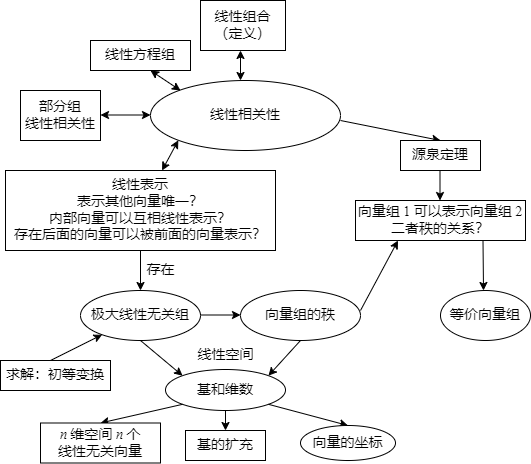
\includegraphics[scale=0.6]{figs/3-1.png}
    \end{figure}

    事实上,与其他内容风格不一样的是,本讲中很大一部分的定理我们都给出了证明,一方面是为了提升阅读体验,防止在初学时就被多个``显然''等词汇困惑,另一方面也是希望读者能够从这些比较规范的证明中得到一些证明的技巧.

    也许读到这里很多读者都会有些迷惑与焦急——为什么我们仿佛在学习很多看起来十分抽象而且似乎没什么实际应用的知识呢?或许我们需要在这里给读者一个``定心丸''. 事实上,我们在上一讲中定义的线性空间运算法则就是从一般向量加法数乘运算法则抽象而来的最为抽象和基本的内容,我们仅仅建立在这一基础上,伴随着线性表示、线性扩张、线性相关等概念的提出,导出了(有限维)线性空间都具有一种统一的本质结构描述——基和维数,由此我们从抽象的运算规则走到了比较具体的结构. 在此基础上,我们基本上将单个线性空间的研究完成,之后我们将会讨论线性空间之间的关系——一方面可以定义线性空间之间的运算,我们将在下一讲详细介绍,另一方面可以建立两个线性空间之间的某种映射,在关于这种映射的讨论中我们会发现线性空间的本质结构是维数,甚至基之间的差异都可以完全被遮蔽(只需通过本讲介绍的坐标即可),然后我们对线性空间的认识便可以从某种比较抽象的结构走向大家熟悉的一定长度的向量,接下来便可以定义更为具象的矩阵. 这一路上我们实际上是从最为抽象的内容逐步定义概念,说明定理,走向具象的内容. 不同于一般线性代数从行列式、矩阵开始,这样的思路一定能让读者对线性代数有更为深刻的认识.

\end{summary}

\begin{exercise}
    \exquote[柯西]{给我五个系数,我将画出一头大象;给我六个系数,大象将会摇动尾巴.}

    \begin{exgroup}
        \item 下列命题是否正确?若正确请证明,否则举出反例.
        \begin{enumerate}
            \item 若 $\alpha_1, \ldots, \alpha_m \ (m > 2)$ 线性相关,则其中每一向量都是其余向量的线性组合;

            \item 若 $\alpha_1, \ldots, \alpha_m$ 线性无关,则其中每一向量不是其余向量的线性组合,这个命题的等价命题应如何叙述?

            \item $\alpha_1, \ldots, \alpha_m \ (m > 2)$ 线性无关的充要条件是任意两个向量都线性无关;

            \item  若 $\alpha_1, \alpha_2$ 线性相关,$ \beta_1, \beta_2$ 线性相关,则 $\alpha_1 + \beta_1, \alpha_2 + \beta_2$ 也线性相关;

            \item 若 $\alpha_1, \ldots, \alpha_n$ 线性无关,则 $\alpha_1 + \alpha_2, \alpha_2 + \alpha_3, \ldots, \alpha_{n-1} + \alpha_n, \alpha_n + \alpha_1$ 也线性无关;

            \item 若 $\alpha_1, \alpha_2, \alpha_3$ 线性相关,则 $\alpha_1 + \alpha_2, \alpha_2 + \alpha_3, \alpha_3 + \alpha_1$ 也线性相关;

            \item 设 $B = \{\alpha_1, \alpha_2, \alpha_3\}$ 是 $ \mathbf{R}^3 $ 的一组基,非零向量 $\alpha_0 \in \mathbf{R}^3$,则 $\{\alpha_0 + \alpha_1, \alpha_0 + \alpha_2, \alpha_0 + \alpha_3\}$ (其中三个向量均是非零向量) 也是 $\mathbf{R}^3$ 的一组基;

            \item  设 $B = \{\alpha_1, \alpha_2\}$ 是 $\mathbf{R}^2$ 的一组基,则 $\{\alpha_1 + \alpha_2, \alpha_1 - \alpha_2\}$ 也是 $\mathbf{R}^2$ 的一组基;

            \item 一个有限维线性空间内只含有有限个子空间;

            \item  若 $W_1, W_2$ 是 $ \mathbf{R}^n $ 的两个子空间,$B_1, B_2$ 分别是 $W_1, W_2$ 的基,则存在 $ \mathbf{R}^n $ 的一组基 $B$,使得 $B \supseteq B_1 \cup B_2$。

        \end{enumerate}
        \begin{answer}
            \begin{enumerate}
                \item 错. 反例:$\alpha_1=(1,0),\alpha_2=(2,0),\alpha_3=(0,1)$,则 $\alpha_1,\alpha_2,\alpha_3$ 线性相关而 $\alpha_3$ 不是 $\alpha_1.\alpha_2$ 的线性组合.

                \item 对. 该命题的等价命题(逆否命题)是:若存在一个向量是其余向量的线性组合,则 $\alpha_1,\ldots,\alpha_m$ 线性相关. 这正是定理 3.1 的内容,因而成立.

                \item 错. 反例:$\alpha_1=(1,0),\alpha_2=(0,1),\alpha_3=(1,1)$,则 $\alpha_1,\alpha_2,\alpha_3$ 两两无关,而三者线性相关. 可证两两无关是向量组无关的必要条件.

                \item 错. 反例:$\alpha_1=(1,0),\alpha_2=(0,0),\beta_1=(0,0),\beta_2=(0,1)$,有 $\alpha_1,\alpha_2$ 相关,$\beta_1,\beta_2$ 相关,而 $\alpha_1+\beta_1$ 与 $\alpha_2+\beta_2$ 线性无关.

                \item 错. 若 $\alpha_1,\ldots,\alpha_n$ 线性无关,有
                    \[\lambda_1\alpha_1+\cdots+\lambda_n\alpha_n\implies\lambda_1=\lambda_2=\cdots=\lambda_n=0,\]
                    判断 $\alpha_1+\alpha_2,\alpha_2+\alpha_3,\ldots,\alpha_n+\alpha_1$ 是否无关. 设
                    \[\lambda_1'(\alpha_1+\alpha_2)+\cdots+\lambda_n'(\alpha_n+\alpha_1)=0,\]
                    则
                    \[(\lambda_n'+\lambda_1')\alpha_1+(\lambda_1'+\lambda_2')\alpha_2+\cdots+(\lambda_{n-1}'+\lambda_{n}')\alpha_n=0,\]
                    则
                    \[\begin{cases} \begin{aligned}
                                \lambda_n'+\lambda_1'       & = 0               \\
                                                            & \vdotswithin{ = } \\
                                \lambda_{n-1}'+\lambda_{n}' & = 0               \\
                            \end{aligned} \end{cases}.\]
                    解该方程可得 $\lambda_n'=(-1)^n\lambda_1'$,因此当 $n$ 为偶数时,上述方程组有非零解,则向量组相关,而当 $n$ 为奇数时,向量组无关. 综上,该命题不成立.

                \item 对. 由定理 3.1,不妨设 $\alpha_3$ 可由 $\alpha_1,\alpha_2$ 线性表示,则 $\alpha_1+\alpha_2,\alpha_2+\alpha_3,\alpha_3+\alpha_1$ 均可由 $\alpha_1,\alpha_2$ 线性表示,再由定理 3.3 可知,$\alpha_1+\alpha_2,\alpha_2+\alpha_3,\alpha_3+\alpha_1$ 线性相关.

                \item 错. 反例:取 $\alpha_0=\alpha_1-\alpha_2-\alpha_3$,则 $\alpha_0+\alpha_1=(\alpha_0+\alpha_2)+(\alpha_0+\alpha_3)$,三者线性相关,不是 $\mathbf{R}^3$ 的基.

                \item 对. 判断 $\alpha_1+\alpha_2$ 与 $\alpha_1-\alpha_2$ 是否无关.
                    \[\lambda_1(\alpha_1+\alpha_2)+\lambda_2(\alpha_1-\alpha_2)=0,\]
                    则有$(\lambda_1+\lambda_2)\alpha_1+(\lambda_1-\lambda_2)\alpha_2=0$,则 $\lambda_1+\lambda_2=0,\lambda_1-\lambda_2=0\implies \lambda_1=\lambda_2=0$,因此线性无关且个数等于维数,是一组基.

                \item 错. 反例:$\mathbf{R}^2$ 中过原点的直线 $L_0$ 是 $\mathbf{R}^2$ 的一个子空间. 显然这样的直线有无数条.

                \item 错. 反例:$\mathbf{R}^3$ 中,子空间 $W_1=\spa(e_1,e_2)$,$W_2=\spa(e_1+e_2,e_3)$,则 $B_1\cup B_2=\{e_1,e_2,e_3,e_1+e_2\}$,显然 $\mathbf{R}^3$ 中的任一组基都不可能包含四个元素.
            \end{enumerate}
        \end{answer}

        \item 证明:如果向量组线性相关,把每个向量去掉$m$个位置一致的分量,得到的缩短组仍线性相关;如果向量组线性无关,把每个向量添加$m$个位置一致的分量,得到的缩短组仍线性无关;
        \begin{answer}
            \begin{enumerate}
                \item 若向量组线性相关,则对应该方程组有无穷多解. 去掉 $m$ 个分量,相当于删去该方程组中的任意 $m$ 行方程,依然有无穷多解. 这是因为对于原方程组的任意一个解,将其带入被削减后的方程组也依然成立. 故线性相关得证.

                \item 若向量组线性无关,对应原方程组仅有唯一解,也就是全零解. 增加 $m$ 个分量相当于增加 $m$ 个方程,依然只有唯一解,因为若出现非零解,代入原方程组对应的方程中不会成立,矛盾. 故线性无关得证.
            \end{enumerate}
        \end{answer}

        \item $a$取何值时,$\beta_1=(1,3,6,2)^\mathrm{T},\beta_2=(2,1,2,-1)^\mathrm{T},\beta_3=(1,-1,a,-2)^\mathrm{T}$线性无关?
        \begin{answer}
            方程组:$x_1\beta_1+x_2\beta_2+x_3\beta_3=0$ 系数矩阵
            \[\begin{pmatrix}
                    1 & 2  & 1  \\
                    3 & 1  & -1 \\
                    6 & 2  & a  \\
                    2 & -1 &
                    -2\end{pmatrix}\rightarrow\begin{pmatrix}
                    1 & 2   & 1   \\
                    0 & -5  & -4  \\
                    0 & -10 & a-6 \\
                    0 & -6  & -4
                \end{pmatrix}\rightarrow\begin{pmatrix}
                    1 & 2  & 1   \\
                    0 & -5 & -4  \\
                    0 & 0  & a+2 \\
                    0 & 0  & 0
                \end{pmatrix},\]
            仅全零解的条件是 $a\neq-2$,此时向量组线性无关.
        \end{answer}

        \item 设$\alpha_1,\alpha_2,\ldots,\alpha_n\in\mathbf{F}^n$. 证明:$\alpha_1,\alpha_2,\ldots,\alpha_n$线性无关的充要条件是$\mathbf{F}^n$中任一向量都可以由它们线性表示.
        \begin{answer}
            \begin{enumerate}
                \item 必要性:$\alpha_1,\ldots,\alpha_n$ 线性无关,对于 $F^n$ 中的任一向量 $\beta$, $\alpha_1,\ldots,\alpha_n,\beta$ 的向量个数大于维数 $n$,则线性相关. 由定理 3.2,$\beta$ 可被 $\alpha_1,\ldots,\alpha_n$ 唯一表示.

                \item 充分性:由于 $F^n$ 中任意向量均可被 $\alpha_1,\ldots,\alpha_n$ 线性表示,并且向量个数等于维数. 则 $\alpha_1,\ldots,\alpha_n$ 是 $F^n$ 的一组基. 则 $\alpha_1,\ldots,\alpha_n$ 线性无关.

                      $^*$ 更详细的证明:对于 $F^n$ 的一组基 $e_1,\ldots,e_n$,其可被 $\alpha_1,\ldots,\alpha_n$ 表示. 若 $\alpha_1,\ldots,\alpha_n$ 线性相关,不妨设 $\alpha_n$ 可被 $\alpha_1,\ldots,\alpha_{n-1}$ 表示,则有 $e_1,\ldots,e_n$ 可被 $\alpha_1,\ldots,\alpha_{n-1}$ 表示. 由于 $e_1,\ldots,e_n$ 线性无关. 根据定理 3.3,$n\leqslant n-1$,矛盾. 因此得证.
            \end{enumerate}
        \end{answer}

        \item 设$S_1=\{\alpha_1,\ldots,\alpha_s\},S_2=\{\beta_1,\ldots,\beta_t\}$是向量空间$V$的两个线性无关的子集,证明:$\alpha_1,\ldots,\alpha_s,\beta_1,\ldots,\beta_t$线性无关$\iff \spa(S_1)\cap \spa(S_2)=\{0\}$.
        \begin{answer}
            \begin{enumerate}
                \item 必要性:对于 $\forall v\in\spa(S_1) \cap \spa(S_2)$ 有 $v=a_1\alpha_1+\cdots+a_s\alpha_s=b_1\beta_1+\cdots+b_t\beta_t$. 由于 $\alpha_1,\ldots,\alpha_s,\beta_1,\ldots,\beta_t$ 线性无关 $\implies a_1=\cdots=a_s=b_1=\cdots=b_t=0$,则 $v=0$,即 $\spa(S_1)\cap\spa(S_2)=\{0\}$.

                \item 充分性:考虑反证法. 如果 $\alpha_1,\ldots,\alpha_s,\beta_1,\ldots,\beta_t$ 线性相关,则存在不全为零的系数使得 $a_1\alpha_1+\cdots+a_s\alpha_s+b_1\beta_1\cdots+b_t\beta_t=0$. 因此存在一个向量 $v=a_1\alpha_1+\cdots+a_s\alpha_s=-(b_1\beta_1\cdots+b_t\beta_t)\neq 0$ 且 $v\in\spa(S_1),v\in\spa(S_2)$. 即存在非零向量 $v$ 属于 $\spa(S_1),v\in\spa(S_2)$,矛盾!则充分性得证.
            \end{enumerate}
        \end{answer}

        \item 完成 \autoref{lem:初等行变换不改变列的线性相关性} 其它两种初等行变换的证明.
        \begin{answer}
            设矩阵为
            \[
                \begin{pmatrix}
                    a_{11} & a_{12} & \cdots & a_{1n} \\
                    a_{21} & a_{22} & \cdots & a_{2n} \\
                    \vdots & \vdots & \ddots & \vdots \\
                    a_{m1} & a_{m2} & \cdots & a_{mn}
                \end{pmatrix},
            \]

            \begin{enumerate}
                \item 对其进行倍乘行变换,即将第 $i$ 行乘以 $c$,那么第 $i$ 行会变为 $c a_{i1}, c a_{i2}, \ldots, c a_{in}$,而其他行不变. 记原先矩阵的列向量为 $S_A = \{\alpha_1,\alpha_2,\ldots,\alpha_n\}$,变换后的矩阵列向量为 $S_B = \{\beta_1,\beta_2,\ldots,\beta_n\}$.

                    先证 $S_A$ 线性相关 $\implies S_B$ 线性相关:若 $S_A$ 线性相关,则存在不全为零的系数 $x_1, x_2, \ldots, x_n$ 使得 $x_1 \alpha_1 + x_2 \alpha_2 + \cdots + x_n \alpha_n = 0$. 由于 $S_B$ 与 $S_A$ 只有第 $i$ 行不同,我们仅需要判断第 $i$ 行中的元素在系数 $x_1, x_2, \ldots, x_n$ 下的线性组合是否为 $0$ 即可. 事实上我们有 $x_1 c a_{i1} + x_2 c a_{i2} + \cdots + x_n c a_{in} = c(x_1 a_{i1} + x_2 a_{i2} + \cdots + x_n a_{in}) = 0$,故 $S_B$ 线性相关.

                    再证 $S_B$ 线性相关 $\implies S_A$ 线性相关:若 $S_B$ 线性相关,由于倍乘行变换保证 $c \neq 0$,故从 $S_B$ 到 $S_A$ 相当于做一次将第 $i$ 行乘以 $\frac{1}{c}$ 的行变换,同理可得 $S_A$ 线性相关.

                    因此,对矩阵做倍乘行变换不改变矩阵的列的线性相关性.

                \item 对其进行对换行变换,即将第 $i$ 行与第 $j$ 行交换,其他行不变. 记原先矩阵的列向量为 $S_A = \{\alpha_1,\alpha_2,\ldots,\alpha_n\}$,变换后的矩阵列向量为 $S_B = \{\beta_1,\beta_2,\ldots,\beta_n\}$.

                    先证 $S_A$ 线性相关 $\implies S_B$ 线性相关:若 $S_A$ 线性相关,则存在不全为零的系数 $x_1, x_2, \ldots, x_n$ 使得 $x_1 \alpha_1 + x_2 \alpha_2 + \cdots + x_n \alpha_n = 0$. 由于 $S_B$ 与 $S_A$ 只有第 $i$ 行与第 $j$ 行不同,我们仅需要判断第 $i$ 行与第 $j$ 行中的元素在系数 $x_1, x_2, \ldots, x_n$ 下的线性组合是否均为 $0$ 即可. 事实上由原先第 $i$($j$)行的元素在 $x_1, x_2, \ldots, x_n$ 下的线性组合为 $0$ 即可得到变换后第 $j$($i$)行的元素的线性组合为 $0$,故 $S_B$ 线性相关.

                    再证 $S_B$ 线性相关 $\implies S_A$ 线性相关:若 $S_B$ 线性相关,从 $S_B$ 到 $S_A$ 相当于再做一次相同的对换行变换,同理有 $S_A$ 线性相关.

                    因此,对矩阵做对换行变换不改变矩阵的列的线性相关性.
            \end{enumerate}
        \end{answer}

        \item 已知$\alpha_1=(1,2,4,3),\alpha_2=(1,-1,-6,6),\alpha_3=(-2,-1,2,-9),\alpha_4=(1,1,-2,7),\beta=(4,2,4,a)$.
        \begin{enumerate}
            \item 求子空间$\spa(\alpha_1,\alpha_2,\alpha_3,\alpha_4)$的维数和一组基;

            \item 求$a$的值使得$\beta\in W$,并求$\beta$在 (1) 所选基下的坐标.
        \end{enumerate}
        \begin{answer}
            \begin{enumerate}
                \item 也就是求 $\alpha_1,\alpha_2,\alpha_3,\alpha_4$ 的极大线性无关组. 利用讲义中所述求法:方程组
                      \[ a_1\alpha_1+\cdots+a_4\alpha_4=0 \]
                      对应系数矩阵 $\begin{pmatrix}
                              1 & 1  & -2 & 1  \\
                              2 & -1 & -1 & 1  \\
                              4 & -6 & 2  & -2 \\
                              3 & 6  & -9 & 7\end{pmatrix}$. 化简为行阶梯型:$\begin{pmatrix}
                              1 & 1  & -2 & 1  \\
                              0 & -3 & 3  & -1 \\
                              0 & 0  & 0  & 3  \\
                              0 & 0  & 0  & 0\end{pmatrix}$,因此 $\alpha_1,\alpha_2,\alpha_3,\alpha_4$ 有非零解,这四个向量线性相关. (其实此处已知矩阵秩为 3,即维数是 3).

                      再选取 $\alpha_1,\alpha_2,\alpha_4$ 来求解方程 $a_1\alpha_1+a_2\alpha_2+a_4\alpha_4=0$:
                      \[\begin{pmatrix}
                              1 & 1  & 1  \\
                              2 & -1 & 1  \\
                              4 & -6 & -2 \\
                              3 & 6  & 7\end{pmatrix}\rightarrow\begin{pmatrix}
                              1 & 1  & 1  \\
                              0 & -3 & -2 \\
                              0 & 0  & 2  \\
                              0 & 0  & 0\end{pmatrix},\]
                      因此该方程组只有全零解,即 $\alpha_1,\alpha_2,\alpha_4$ 是$\alpha_1,\alpha_2,\alpha_3,\alpha_4$的极大线性无关组. 则 $\spa(\alpha_1,\alpha_2,\alpha_4)$ 的维数是 3. 一组基是 $\alpha_1,\alpha_2,\alpha_4$ .

                \item 也就是 $a_1\alpha_1+\cdots+a_4\alpha_4=\beta$有解:增广矩阵 $\begin{pmatrix}
                              1 & 1  & -2 & 1  & 4 \\
                              2 & -1 & -1 & 1  & 2 \\
                              4 & -6 & 2  & -2 & 4 \\
                              3 & 6  & -9 & 7  & a\end{pmatrix}$化为 $\begin{pmatrix}
                              1 & 1  & -2 & 1         & 4   \\
                              0 & -3 & 3  & -1        & -6  \\
                              0 & 0  & 0  & -\frac 83 & 8   \\
                              0 & 0  & 0  & 0         & a-9\end{pmatrix}$,若方程有解,则 $a=9$. 求坐标,取 $x_3=0$ 代入得 $\beta=4\alpha_1+3\alpha_2-3\alpha_4$.
            \end{enumerate}
        \end{answer}

        \item 求解子空间 $V_1 = \{(a,0,b) \mid a,b \in \mathbf{R}\}$ 和 $V_2 = \{(a,2a,b) \mid a,b \in \mathbf{R}\}$ 的基和维数.
        \begin{answer}

        \end{answer}

        \item 证明:$B=\{1,x-a,(x-a)^2\}\enspace(a\neq 0)$是$\mathbf{R}[x]_3$的一组基,并求$\mathbf{R}[x]_3$的自然基$\{1,x,x^2\}$中每个向量关于基$B$的坐标.
        \begin{answer}
            只需证明 $B$ 线性无关即可. $\lambda_1+\lambda_2(x_a)+\lambda_3(x-a)^2$求导,增加方程数得到
            \begin{gather*}
                \lambda_2+2\lambda_3x=0, \\
                2\lambda_3=0,
            \end{gather*}
            则 $\lambda_1=\lambda_2=\lambda_3$,线性无关得证. 又 $B$ 中向量个数等于 $R[x]_3$ 维数. 则 $B$ 是一组基. $1=1 \cdot 1+0 \cdot (x-a)+0\times(x-a)^2$ ,即 $(1,0,0)$;$x=a \cdot 1+1 \cdot (x-a)+0\times(x-a)^2$ ,即 $(a,1,0)$;$x^2=a^2 \cdot 1+2a \cdot (x-a)+1\times(x-a)^2$ ,即 $(a^2,2a,1)$.
        \end{answer}

        \item 已知向量组$A=\{\alpha_1,\alpha_2,\alpha_3\},\enspace B=\{\alpha_1,\alpha_2,\alpha_3,\alpha_4\},\enspace C=\{\alpha_1,\alpha_2,\alpha_3,\alpha_5\}$的秩分别为$r(A)=r(B)=3,\enspace r(C)=4$. 证明:$\{\alpha_1,\alpha_2,\alpha_3,\alpha_5-\alpha_4\}$的秩为4.
        \begin{answer}
            等价于证明 $\alpha_1,\alpha_2,\alpha_3,\alpha_5-\alpha_4$ 线性无关. 即求解
            \begin{equation}
                \lambda_1\alpha_1+\lambda_2\alpha_2+\lambda_3\alpha_3+\lambda_4(\alpha_5-\alpha_4)=0. \tag{*} \label{eq:3:A.10}
            \end{equation}

            由于 $r(A)=r(B)=3$ 可得 $A$ 线性无关. $B$ 线性相关. 由定理 3.2 得 $\alpha_4$ 可由 $\alpha_1,\alpha_2,\alpha_3$ 唯一表示:$\alpha_4=\mu_1\alpha_1+\mu_2\alpha_2+\mu_3\alpha_3$. 则代入 (\ref*{eq:3:A.10}) 式. 有
            \[(\lambda_1-\mu_1\lambda_4)\alpha_1+(\lambda_2-\mu_2\lambda_4)\alpha_2+(\lambda_3-\mu_3\lambda_4)\alpha_3+\lambda_4\alpha_5=0,\]
            因为 $r(C)=4$,$\alpha_1,\alpha_2,\alpha_3,\alpha_5$ 线性无关. 有 $\lambda_4=0,\lambda_1=\mu_1\lambda_4=0,\lambda_2=\mu_2\lambda_4=0,\lambda_3=\mu_3\lambda_4=0$. 故 $\alpha_1,\alpha_2,\alpha_3,\alpha_5-\alpha_4$ 线性无关. 原题得证.
        \end{answer}

        \item 设向量组$\alpha_1,\alpha_2,\ldots,\alpha_s$的秩为$r$. 在其中任取$m$个向量$\alpha_{i1},\alpha_{i2},\ldots,\alpha_{im}$,证明:向量组$\alpha_{i1},\alpha_{i2},\ldots,\alpha_{im}$的秩$\geqslant r+m-s$.
        \begin{answer}
            相当于从 $\alpha_1,\ldots,\alpha_s$ 向量中选取 $s-m$ 个向量丢弃,剩余向量的秩:
            \[r(\alpha_{i1},\ldots,\alpha_{im})\geqslant r-(s-m) =r+m-s.\]
        \end{answer}

        \item 已知$\alpha_1,\alpha_2,\ldots,\alpha_n$线性无关,而$\alpha_1,\alpha_2,\ldots,\alpha_n,\beta,\gamma$线性相关. 证明:要么$\beta,\gamma$可以由$\alpha_1,\alpha_2,\ldots,\alpha_n$线性表示,要么$\alpha_1,\alpha_2,\ldots,\alpha_n,\beta$与$\alpha_1,\alpha_2,\ldots,\alpha_n,\gamma$等价.
        \begin{answer}
            方程:$\lambda_1\alpha_1+\cdots+\lambda_n\alpha_n+\lambda_{n+1}\beta+\lambda_{n+2}\gamma=0$,显然 $\lambda_{n+1},\lambda_{n+2}$ 不全为零. 否则与 $\alpha_1,\ldots,\alpha_n$ 线性无关矛盾.
            \begin{enumerate}
                \item 若 $\lambda_{n+1}=0,\lambda_{n+2}\neq 0$,则 $\gamma$ 可被 $\alpha_1,\ldots,\alpha_n$ 表示. 若 $\lambda_{n+1}\neq0,\lambda_{n+2}=0$, 则 $\beta$ 可被 $\alpha_1,\ldots,\alpha_n$ 表示.

                \item 若 $\lambda_{n+1}\lambda_{n+2}\neq 0$ ,则有
                      \begin{gather*}
                          \beta=-\frac 1{\lambda_{n+1}}(\lambda_1\alpha_1+\cdots+\lambda_n\alpha_n+\lambda_{n+2}\gamma), \\
                          \gamma=-\frac 1{\lambda_{n+2}}(\lambda_1\alpha_1+\cdots+\lambda_n\alpha_n+\lambda_{n+1}\beta).
                      \end{gather*}
                    两组向量可以相互表示. 两者等价. 综上原题得证.
            \end{enumerate}
        \end{answer}
    \end{exgroup}

    \begin{exgroup}
        \item 已知$\alpha_1\neq 0$,则$\alpha_1,\alpha_2,\ldots,\alpha_n$线性相关的充要条件是存在$i\enspace(2 \leqslant i \leqslant n)$使得$\alpha_i$可由$\alpha_1,\alpha_2,\ldots,\alpha_{i-1}$线性表示,且表示法唯一.
        \begin{answer}
            充分性显然成立,下证必要性:由于 $\alpha_1,\ldots,\alpha_n$ 线性相关,则存在 $m$,其能使得 $\alpha_1,\ldots,\alpha_m$ 线性无关的最大下标,有 $1\leqslant m<n$. 因此 $i=m+1$,$\alpha_1,\ldots,\alpha_{i-1}$ 线性无关,$\alpha_1,\ldots,\alpha_i$ 线性相关. 可得 $\alpha_i$ 可被 $\alpha_1,\ldots,\alpha_{i-1}$ 唯一表示.
        \end{answer}

        \item 证明以下两个结论:
        \begin{enumerate}
            \item 设$U$和$W$都是$V$的非零子空间,如果$U\subseteq W$,那么$\dim U \leqslant \dim W$;

            \item 设$U$和$W$都是$V$的非零子空间,$U\subseteq W$,且$\dim U = \dim W$,则$U = W$.
        \end{enumerate}
        \begin{answer}
            \begin{enumerate}
                \item 设 $U$ 的一组基为 $u_1,\ldots,u_m$,$W$ 的一组基为 $w_1,\ldots,w_n$. 由于 $U\subseteq W$,则 $u_1,\ldots,u_m$ 可由 $w_1,\ldots,w_n$ 线性表示,且 $u_1,\ldots,u_m$ 线性无关. 由定理 3.3 的等价命题可得 $m\leqslant n$,则 $m=\dim U\leqslant\dim W=n$ 的得证.

                \item 因为 $\dim U=\dim W$,则 $u_1,\ldots,u_m$ 也是 $W$ 的一组基. 则 $W$ 的任意向量均可由 $u_1,\ldots,u_m$ 表示,可得 $W\subseteq U$,而 $U\subseteq W$,故有 $U=W$ 得证.
            \end{enumerate}
        \end{answer}

        \item 设向量组$\alpha_1,\alpha_2,\ldots,\alpha_n$线性无关. 证明:在向量组$\beta,\alpha_1,\alpha_2,\ldots,\alpha_n$中至多有一个向量$\alpha_i\enspace(1 \leqslant i \leqslant r)$可被其前面的$i$个向量$\beta,\alpha_1,\alpha_2,\ldots,\alpha_{i-1}$线性表示.
        \begin{answer}
            反证法. 若存在两个向量 $\alpha_i,\alpha_j$ 可被前面的向量表示,即
            \begin{gather*}
                \alpha_i=\lambda_0\beta+\lambda_1\alpha_1+\cdots+\lambda_{i-1}\alpha_{i-1}, \\
                \alpha_j=\mu_0\beta+\mu_1\alpha_1+\cdots+\mu_{j-1}\alpha_{j-1}.
            \end{gather*}
            如果 $\lambda_0$ 或者 $\mu_0$ 为 0,则有向量组中的 $\alpha_i$ 或 $\alpha_j$ 可被其他向量线性表示,则该向量组相关,这与条件矛盾. 若 $\lambda_0$ 与 $\mu_0$ 均不为 0,等式可化为
            \begin{gather*}
                \frac 1{\lambda_0}\alpha_i=\beta+\frac{\lambda_1}{\lambda_0}\alpha_1+\cdots+\frac{\lambda_{i-1}}{\lambda_0}\alpha_{i-1}, \\
                \frac 1{\mu_0}\alpha_j=\beta+\frac{\mu_1}{\mu_0}\alpha_1+\cdots+\frac{\mu_{j-1}}{\mu_0}\alpha_{j-1}.
            \end{gather*}
            不妨设 $i>j$. 相减得
            \[\frac 1{\lambda_0}\alpha_i=\left(\frac{\lambda_1}{\lambda_0}-\frac{\mu_1}{\mu_0}\right)\alpha_1+\cdots+\left(\frac{\lambda_i}{\lambda_0}+\frac 1{\mu_0}\right)\alpha_j+\frac{\lambda_{i-1}}{\lambda_0}\alpha_{i-1},\]
            则 $\alpha_i$ 可被其他向量线性表示,因此向量组线性相关,与条件矛盾. 综上,至多有一个向量 $\alpha_i$ 可被前面的相邻线性表示.
        \end{answer}

        \item 证明:$1,e^{\lambda_1\cdot x},e^{\lambda_2\cdot x}$($\lambda_1\neq\lambda_2$且均不为0)线性无关.
        \begin{answer}
            考虑使用求导构造更多方程.
            \[\begin{cases}
                    k_0+k_1\cdot e^{\lambda_1 x}+k_2\cdot e^{\lambda_2 x}=0               \\
                    k_1\lambda_1\cdot e^{\lambda_1 x}+k_2\lambda_2\cdot e^{\lambda_2 x}=0 \\
                    k_1\lambda_1^2\cdot e^{\lambda_1 x}+k_2\lambda_2^2\cdot e^{\lambda_2 x}=0
                \end{cases},\]
          由后两式可知$k_1k_2(\lambda_1-\lambda_0)=0$. 又 $\lambda_1\neq\lambda_2$,故$k_1=k_2=0$,代回第一式得 $k_0=0$,则 $1,e^{\lambda_1x},e^{\lambda_2x}$ 线性无关,得证.
        \end{answer}

        \item 设线性空间$V(\mathbf{F})$中,向量$\beta$是$\alpha_1,\ldots,\alpha_r$的线性组合,但不是$\alpha_1,\ldots,\alpha_{r-1}$的线性组合. 证明:$\spa(\alpha_1,\ldots,\alpha_{r-1},\alpha_r)=\spa(\alpha_1,\ldots,\alpha_{r-1},\beta)$.
        \begin{answer}
            只需证明 $\alpha_r$ 可以被 $\alpha_1,\ldots,\alpha_{r-1},\beta$ 表示即可. 由于 $\beta$ 是 $\alpha_1,\ldots,\alpha_{r-1}$ 的线性组合,若 $\lambda_r=0$,则 $\beta$ 是 $\alpha_1,\ldots,\alpha_{r-1}$ 的线性组合. 这与条件矛盾. 因此 $\alpha_r=-\vspace{1ex}\dfrac 1{\lambda_r}(\lambda_1\alpha_1+\cdots+\lambda_{r-1}\alpha_{r-1}-\beta)$,则这两组向量等价. $\spa(\alpha_1,\ldots,\alpha_{r-1},\alpha_r)=\spa(\alpha_1,\ldots,\alpha_{r-1},\beta)$ 得证.
        \end{answer}

        \item \label{item:3:正实数线性空间}
        设$\mathbf{R}^+$是所有正实数组成的集合,加法和数乘定义如下:
        \[ \forall a,b \in \mathbf{R}_+,\enspace k\in \mathbf{R}\colon\enspace a\oplus b = ab,\enspace k\odot a = a^k \]
        则 $\mathbf{R}^+$关于这一加法和数乘构成一个实线性空间. 求$\mathbf{R}^+$的一组基.
        \begin{answer}
            分析该实线性空间,可以看出加法单位元为 1,数乘单位元为 1. 我们给出一组基:$e$,其中 $e$ 为自然对数的底数. 当然, 2,3 或者 10 都可以作为一组基. 接下来我们验证 $e$ 是 $\mathbf{R}^+$ 的基:$\forall a\in \mathbf{R}^+,\exists k=\ln a\in\mathbf{R}$,满足 $k\odot e=e^k=a$,则 $\spa(e)=\mathbf{R}^+$ 成立. 由于该向量组只有一个元素,且并非设该空间的零元 1,则 $e$ 是线性无关的. 得证.
        \end{answer}
    \end{exgroup}

    \begin{exgroup}
        \item 已知$m$个向量$\alpha_1,\alpha_2,\ldots,\alpha_m$线性相关,但其中任意$m-1$个都线性无关,证明:
        \begin{enumerate}
            \item 若$k_1\alpha_1+\cdots+k_m\alpha_m=0$,则$k_1,\ldots,k_m$全为0或全不为0;

            \item 若以下等式成立
                  \begin{align*}
                      k_1\alpha_1+\cdots+k_m\alpha_m & =0 \\
                      l_1\alpha_1+\cdots+l_m\alpha_m & =0
                  \end{align*}
                  其中$l_1\neq 0$,证明:$\dfrac{k_1}{l_1}=\cdots=\dfrac{k_m}{l_m}$.
        \end{enumerate}
        \begin{answer}
            \begin{enumerate}
                \item 若 不全为 0. 不妨设设至少有 $k_i=0$,则有 $k_1\alpha_1+\cdots+k_{i-1}\alpha_{i-1}+k_{i+1}\alpha_{i+1}+\cdots+k_m\alpha_m=0$,并且系数不全为 0. 因此 $\alpha_1,\ldots,\alpha_{i-1},\alpha_{i+1},\ldots,\alpha_m$ 这 $m-1$ 个向量相关,与题设矛盾. 则原题得证.

                \item $l_1\neq 0$,则 $l_2,\ldots,l_m$ 均不为 0.
                      \begin{enumerate}
                          \item 若 $k_1=\cdots=k_m=0$. 原式显然成立.

                          \item 若 $k_1,\ldots,k_m$ 不全为 0. 则
                                \begin{gather*}
                                    l_1(k_1\alpha_1+\cdots+k_m\alpha_m)=0, \\
                                    k_1(l_1\alpha_1+\cdots+l_m\alpha_m)=0.
                                \end{gather*}
                                两式相减,得
                                \[(k_2l_1-k_1l_2)\alpha_2+\cdots+(k_ml_1-k_1l_m)\alpha_m=0,\]
                                因为 $\alpha_2,\ldots,\alpha_m$ 线性无关. 则以上系数均为 0. 故$\dfrac {k_2}{l_2}=\dfrac {k_1}{l_1},\ldots,\dfrac {k_m}{l_m}=\dfrac {k_1}{l_1}$. 得证.
                      \end{enumerate}
            \end{enumerate}
        \end{answer}

        \item (替换定理)设$\alpha_1,\alpha_2,\ldots,\alpha_r$线性无关,且可以被$\beta_1,\beta_2,\ldots,\beta_n$线性表示,则可以将$\beta_1,\beta_2,\ldots,\beta_n$中的$r$个向量替换成$\alpha_1,\alpha_2,\ldots,\alpha_r$后得到与$\beta_1,\beta_2,\ldots,\beta_n$等价的新向量组(注:可以使用数学归纳法证明).
        \begin{answer}
            利用递推法:当 $r=1$ 时,由于 $\alpha_1$ 线性无关,可得 $\alpha_1\neq 0$. 设 $\alpha_1=\lambda_1\beta_1+\cdots+\lambda_n\beta_n$,则至少存在一个 $\lambda_i\neq 0$,不妨设 $\lambda_1\neq 0$,因此有 $\beta_1=-\vspace{1ex}\dfrac 1{\lambda_1}(-\alpha_1+\lambda_2\beta_2+\cdots+\lambda_n\beta_n)$,故 $\beta_1,\ldots,\beta_n$ 与 $\alpha_1,\beta_2,\ldots,\beta_n$ 等价.

            当 $r=2$ 时,由于 $\alpha_1,\alpha_2$ 无关. 有 $\alpha_1\alpha_2\neq 0$. 根据 $r=1$ 的情况,不妨设 $\beta_1,\ldots,\beta_n$ 与 $\alpha_1,\beta_2,\ldots,\beta_n$ 等价. 因此 $\alpha_2$ 可由 $\alpha_1,\beta_2,\ldots,\beta_n$ 表出:
            \[\alpha_2=\mu_1\alpha_1+\mu_2\beta_2+\cdots+\mu_n\beta_n.\]
            由于 $\alpha_1,\alpha_2$ 无关,故 $\mu_2,\ldots,\mu_n$ 至少有一个非零的数. 不妨设 $\mu_2\neq 0$,同上可得$\alpha_1,\alpha_2,\beta_3,\ldots,\beta_n$ 就与 $\alpha_1,\beta_2,\ldots,\beta_n$ 等价,也与$\beta_1,\beta_2,\ldots,\beta_n$ 等价. 综上,通过递推可知,对正整数 $r$,上述结论依然成立.
        \end{answer}

        \item 设线性空间$V=\mathbf{F}^n$. 证明:
        \begin{enumerate}
            \item 存在$V$的子空间$W$,使得$W$的任一非零向量的分量均不为0;

            \item 若$V$的子空间$W$的任一非零向量的分量均不为0,则$\dim W=1$;

            \item 若$V$的子空间$W$的任一非零向量的零分量个数均不超过$r$,则$\dim W \leqslant r+1$.
        \end{enumerate}
        \begin{answer}
            \begin{enumerate}
                \item $\alpha=(1,1,\ldots,1)^{\mathrm{T}}, W=\spa(\alpha)$,显然 $W$ 是满足条件的一维子空间.

                \item 考虑反证法:若 $\dim W>1$,则 $W$ 中存在线性无关的两向量. 由条件,
                      \[a_1,\ldots,a_n,b_1,\ldots,b_n\neq 0,\]
                      可设 $a_1=kb_1,k\in F$,因此 $\alpha-k\beta=(0,a_2-kb-2,\ldots,a_n-kb_n)^{\mathrm{T}}\in W$. 且由于 $\alpha,\beta$ 无关,$\alpha-k\beta\neq 0$ 但存在分量为 0,这与条件矛盾. 故 $\dim W=1$.

                \item 考虑反证法:若 $\dim W>r+1$,则存在 $r+2$ 个线性无关的向量,设为
                      \begin{align*}
                          \alpha_1     & = (a_{11},a_{12},\ldots,a_{1(r+1)},\ldots,a_{1n})^{\mathrm{T}},                 \\
                                       & \vdotswithin{ = }                                                              \\
                          \alpha_{r+2} & = (a_{(r+2)1},a_{(r+2)2},\ldots,a_{(r+2)(r+1)},\ldots,a_{(r+2)n})^{\mathrm{T}}.
                      \end{align*}
                      取这些向量的前 $r+1$ 个分量组成新的向量组:
                      \begin{align*}
                          \beta_1     & = (a_{11},a_{12},\ldots,a_{1(r+1)})^{\mathrm{T}},             \\
                                      & \vdotswithin{ = }                                            \\
                          \beta_{r+2} & = (a_{(r+2)1},a_{(r+2)2},\ldots,a_{(r+2)(r+1)})^{\mathrm{T}}.
                      \end{align*}
                      由于 $\beta_1,\ldots,\beta_{r+2}$ 是 $r+2$ 个 $r+1$ 维向量,其必然线性相关,则存在不全为 0 的系数 $\lambda_1,\ldots,\lambda_{r+2}$,$\lambda_1\beta_1+\cdots+\lambda_{r+2}\beta_{r+2}=0$.  由于 $\alpha_1,\ldots,\alpha_{r+2}$ 线性无关知:$\lambda_1\alpha_1+\cdots+\lambda_{r+2}\alpha_{r+2}\neq 0$,且其属于 $W$. 但其前 $r+1$ 个分量均为 0,这与条件矛盾. 故 $\dim W\leqslant r+1$ 得证.
            \end{enumerate}
        \end{answer}

        \item 设 $\mathbf{Q}(\sqrt[3]{2}) = \{a+b\sqrt[3]{2}+c\sqrt[3]{4}\mid a,b,c\in\mathbf{Q}\}$,证明 $\mathbf{Q}(\sqrt[3]{2})$ 是 $\mathbf{Q}$ 上的线性空间并求其维数.
        \begin{answer}
            先证明 $\mathbf{Q}(\sqrt[3]{2})$ 是 $\mathbf{Q}$ 上的线性空间:

            $\mathbf{Q}(\sqrt[3]{2})$ 对通常的加法构成交换群以及其封闭性是显然的,在此不再赘述,下阐述数乘性质:
            \begin{enumerate}
                \item $\forall v = a+b\sqrt[3]{2}+c\sqrt[3]{4} \in \mathbf{Q}(\sqrt[3]{2}), \enspace 1 (a+b\sqrt[3]{2}+c\sqrt[3]{4}) = a+b\sqrt[3]{2}+c\sqrt[3]{4}$;

                \item $\forall v = a+b\sqrt[3]{2}+c\sqrt[3]{4} \in \mathbf{Q}(\sqrt[3]{2}), \forall \lambda, \mu \in \mathbf{Q}, \enspace \lambda(\mu v) = (\lambda \mu) v$;

                \item $\forall v = a+b\sqrt[3]{2}+c\sqrt[3]{4} \in \mathbf{Q}(\sqrt[3]{2}), \forall \lambda, \mu \in \mathbf{Q}, \enspace (\lambda + \mu) v = (\lambda + \mu)a + (\lambda + \mu) b\sqrt[3]{2} + (\lambda + \mu) c\sqrt[3]{4} = \lambda(a+b\sqrt[3]{2}+c\sqrt[3]{4}) + \mu(a+b\sqrt[3]{2}+c\sqrt[3]{4}) = \lambda v + \mu v$;

                \item $\forall v = a_1 + b_1\sqrt[3]{2} + c_1\sqrt[3]{4}, u = a_2 + b_2\sqrt[3]{2} + c_2\sqrt[3]{4} \in \mathbf{Q}(\sqrt[3]{2}), \forall \lambda \in \mathbf{Q}, \enspace \lambda(v+u) = \lambda (a_1 + a_2) + \lambda (b_1 + b_2)\sqrt[3]{2} + \lambda (c_1 + c_2)\sqrt[3]{4} = \lambda (a_1 + b_1\sqrt[3]{2} + c_1\sqrt[3]{4}) + \lambda (a_2 + b_2\sqrt[3]{2} + c_2\sqrt[3]{4}) = \lambda v + \lambda u$;

                \item (封闭性)$\forall v = a+b\sqrt[3]{2}+c\sqrt[3]{4} \in \mathbf{Q}(\sqrt[3]{2}), \forall \lambda \in \mathbf{Q}, \enspace \lambda v = \lambda a + \lambda b\sqrt[3]{2} + \lambda c\sqrt[3]{4} \in \mathbf{Q}(\sqrt[3]{2})$.
            \end{enumerate}
            故 $\mathbf{Q}(\sqrt[3]{2})$ 是 $\mathbf{Q}$ 上的线性空间.

            下求 $\mathbf{Q}(\sqrt[3]{2})$ 的维数. 考虑找 $\mathbf{Q}(\sqrt[3]{2})$ 的一组基,我们给出 $\{1, \sqrt[3]{2}, \sqrt[3]{4}\}$,下证其为 $\mathbf{Q}(\sqrt[3]{2})$ 的一组基:

            \begin{enumerate}
                \item (线性无关)令 $k_1 + k_2 \sqrt[3]{2} + k_3 \sqrt[3]{4} = 0$,其中 $k_1, k_2, k_3 \in \mathbf{Q}$,由于左边只有第一项为有理数,故有 $k_1 = 0$,进而有 $\sqrt[3]{2} (k_2 + k_3 \sqrt[3]{2}) = 0$,又可得到 $k_2 = 0$,并且 $k_3 = 0$. 故 $\{1, \sqrt[3]{2}, \sqrt[3]{4}\}$ 线性无关.

                \item (张成空间)由 $\mathbf{Q}(\sqrt[3]{2})$ 的定义易得.
            \end{enumerate}
            综上,$\mathbf{Q}(\sqrt[3]{2})$ 是 $\mathbf{Q}$ 上的线性空间,且 $\dim \mathbf{Q}(\sqrt[3]{2}) = 3$.

        \end{answer}

        \item 设$\mathbf{K} \subseteq \mathbf{F} \subseteq \mathbf{E}$是三个数域,已知$\mathbf{F}$作为$\mathbf{K}$上的线性空间是$n$维的,$\mathbf{E}$作为$\mathbf{F}$上的线性空间是$m$维的,证明:$\mathbf{E}$作为$\mathbf{K}$上的线性空间是$mn$维的.
        \begin{answer}
            取 $\mathbf{F}(\mathbf{K})$ 的一组基 $f_1, f_2, \ldots, f_n$,$\mathbf{E}(\mathbf{F})$ 的一组基 $e_1, e_2, \ldots, e_m$,下证向量组 $B = \{f_1 e_1, f_2 e_1, \ldots, f_n e_1, f_1 e_2, f_2 e_2, \ldots, f_n e_2, \ldots, f_1 e_m, f_2 e_m, \ldots, f_n e_m\}$ 是 $\mathbf{E}(\mathbf{K})$ 的一组基:

            \begin{enumerate}
                \item (线性无关)令 $k_{11} f_1 e_1 + k_{12} f_2 e_1 + \cdots + k_{1n} f_n e_1 + k_{21} f_1 e_2 + k_{22} f_2 e_2 + \cdots + k_{2n} f_n e_2 + \cdots + k_{m1} f_1 e_m + k_{m2} f_2 e_m + \cdots + k_{mn} f_n e_m = 0$,其中 $k_{ij} \in \mathbf{K}$,则
                    \[
                        \sum_{i=1}^m \left(\sum_{j=1}^n k_{ij} f_j \right) e_i = 0.
                    \]
                    由于 $e_1, e_2, \ldots, e_n$ 是 $\mathbf{E}(\mathbf{F})$ 的一组基 $e_1, e_2, \ldots, e_m$,我们有
                    \[
                        \sum_{j=1}^n k_{ij} f_j = 0, \enspace \forall i = 1, 2, \ldots, m.
                    \]
                    而 $f_1, f_2, \ldots, f_n$ 又是 $\mathbf{F}(\mathbf{K})$ 的一组基,故 $k_{ij} = 0$,即向量组 $B$ 线性无关.

                \item (张成空间)$\forall e = \mu_1 e_1 + \mu_2 e_2 + \cdots + \mu_m e_m \in \mathbf{E} \enspace (\mu_1, \mu_2, \ldots, \mu_m \in \mathbf{F})$,由于 $\mu_i \in \mathbf{F}$,故存在 $k_{ij} \in \mathbf{K}$ 使得 $\mu_i = k_{i1} f_1 + k_{i2} f_2 + \cdots + k_{in} f_n$,于是
                    \[
                        e = \sum_{i=1}^m \left(\sum_{j=1}^n k_{ij} f_j \right) e_i
                          = \sum_{i=1}^m \sum_{j=1}^n k_{ij} f_j e_i.
                    \]
                    故 $e \in \spa B$.
            \end{enumerate}
            综上,$B$ 是 $\mathbf{E}(\mathbf{K})$ 的一组基,故 $\dim \mathbf{E}(\mathbf{K}) = mn$.
        \end{answer}

        \item 延续上一讲对于 $\mathbf{F_4}(\mathbf{Z}_2)$ 的讨论,尝试求 $\mathbf{F_4}$ 在 $\mathbf{Z}_2$ 上的一组基及其维数,以及其中每个元素的坐标表示.
        \begin{answer}

        \end{answer}
    \end{exgroup}
\end{exercise}

\chapter{线性空间的运算}

在前述章节中我们对(有限维)线性空间中的基本概念以及研究的基本问题进行了了解. 事实上,很多时候我们还需要研究不同线性空间进行运算后得到的新集合的性质,本节我们将详细展开讨论这一问题.

\section{线性空间的交、并、和}

\begin{definition}{}{}
    设$W_1,W_2$是线性空间$V(\mathbf{F})$的两个子空间,则
    \begin{align*}
        W_1 \cap W_2 & =\{\alpha \mid \alpha\in W_1 \text{~且~} \alpha\in W_2\}            \\
        W_1 \cup W_2 & =\{\alpha \mid \alpha\in W_1 \text{~或~} \alpha\in W_2\}            \\
        W_1 + W_2    & =\{\alpha_1+\alpha_2 \mid \alpha_1\in W_1,\enspace\alpha_2\in W_2\}
    \end{align*}
    分别称为$W_1$和$W_2$的交、并、和.
\end{definition}

交与并的定义实际上与集合交与并的定义类似,而和的定义可能有些许反直觉. 我们可以通过一个例子来体会为什么要定义子空间的和.
\begin{example}{}{子空间运算}
    在$\mathbf{R}^3$中,我们设
    \[\alpha_1=(0,0,1),\ \alpha_2=(0,1,0),\ \alpha_3=(1,0,0).\]
    令$\mathbf{R}^3$子空间$W_1=\spa(\alpha_1,\alpha_2)$,$W_2=\spa(\alpha_1,\alpha_3)$,则$W_1$实际上是$yOz$平面,$W_2$是$xOz$平面,因此我们根据交与并的概念(实际上就是集合取交集和并集)得到$W_1 \cap W_2=\spa(\alpha_1)$(即$z$坐标轴).

    进一步考察并集,事实上显然$W_1 \cup W_2$得到的集合表示$xOz$和$yOz$平面上所有的点. 事实上我们发现,$W_1 \cup W_2$得到的集合关于向量加法、数乘运算并不封闭,例如只需取$\alpha_2+\alpha_3=(0,1,1)$就不在$W_1 \cup W_2$中,因此不再是$\mathbf{R}^3$的子空间.

    接下来我们考察二者之和. 事实上$W_1+W_2=\mathbf{R}^3$. 原因在于
    \begin{enumerate}
        \item $\forall \beta\in W_1 + W_2$,由子空间和的定义可知有$\beta=\beta_1+\beta_2$,其中$\beta_1\in W_1\subseteq \mathbf{R}^3$,$\beta_2\in W_2\subseteq \mathbf{R}^3$,由于$\mathbf{R}^3$是线性空间,其中元素关于加法运算封闭,因此$\beta=\beta_1+\beta_2\in \mathbf{R}^3$,即$W_1+W_2\subseteq \mathbf{R}^3$;

        \item $\mathbf{R}^3$中任一向量$(x,y,z)$总能写成$(x,y,z)=(0,y,z)+(x,0,0)$的形式,其中$(0,y,z)$在$W_1$中,$(x,0,0)$在$W_2$中,因此根据子空间和的定义可知$\mathbf{R}^3\subseteq W_1 + W_2$成立.
    \end{enumerate}
    综上,我们得到$W_1+W_2=\mathbf{R}^3$.
\end{example}

从上面证明$W_1+W_2=\mathbf{R}^3$的过程中我们可以提炼出证明子空间的和等于某一空间的一般方法:本质而言仍然是证明集合相等,因此证明两边包含即可. 证明子空间的和属于某一空间是平凡的,如上述证明的第一部分;第二部分证明某一空间属于子空间和只需要将该空间中任意向量都可分解为各个子空间中向量的和即可.

事实上,根据\autoref{ex:子空间运算} 我们发现,子空间$W_1$和$W_2$的交与和仍然是线性空间,但是它们的并不是线性空间. 事实上,我们可以证明如下定理:
\begin{theorem}{}{}
    设$W_1,W_2$是线性空间$V(\mathbf{F})$的两个子空间,则
    \begin{enumerate}
        \item $W_1 \cap W_2$是$V$的子空间;

        \item $W_1 + W_2$是$V$的子空间;

        \item $W_1 \cup W_2$为$V$的子空间$\iff W_1 \subseteq W_2$或$W_2 \subseteq W_1 \iff W_1 \cup W_2=W_1+W_2$.
    \end{enumerate}
\end{theorem}

定理前两条的证明见教材74页,第三条我们留作习题供读者练习,因为在考试中有出现过. 前两条还可以进行推广,即$V$的有限个子空间的交与和仍然是$V$的子空间.

除此之外,这一定理也告诉我们为什么需要研究子空间的和而更少研究子空间的并:因为子空间的和仍然是线性空间. 直观理解实际上就是和的定义中出现了两个子空间的向量的加法,而构成子空间的核心就是运算封闭,因此这一定义为子空间的和仍构成子空间提供了保证,因此这一定义也是十分自然的.

下面我们来看一个例子,在例子中我们将给出求子空间的和与交的一般方法:
\begin{example}{}{}
    设 $\alpha_1 = (1, 0, -1, 0)$,$\alpha_2 = (0, 1, 2, 1)$,$\alpha_3 = (2, 1, 0, 1)$,是四维实行向量空间 $V$ 中的向量,他们张成的子空间为 $V_1$;又设向量 $\beta_1 = (-1, 1, 1, 1)$,$\beta_2 = (1, -1, -3, -1)$,$\beta_3 = (-1, 1, -1, 1)$ 张成的子空间为 $V_2$,求 $V_1$ 和 $V_2$ 的交与和的基.
\end{example}

\begin{solution}
    \begin{enumerate}
        \item 方法一.  $V_1 +V_2$ 是由 $\alpha_i$ 和 $\beta_i$ 生成的,因此只需要求出这 $6$ 个向量的极大线性无关组即可. 将这 $6$ 个向量按列分块方式拼成矩阵,并用初等行变换将其化为阶梯形矩阵:
              \begin{align*}
                  \begin{pmatrix}
                      1  & 0 & 2 & -1 & 1  & -1 \\
                      0  & 1 & 1 & 1  & -1 & 1  \\
                      -1 & 2 & 0 & 1  & -3 & -1 \\
                      0  & 1 & 1 & 1  & -1 & 1
                  \end{pmatrix}
                  \xrightarrow{}
                  \begin{pmatrix}
                      1 & 0 & 2 & -1 & 1  & -1 \\
                      0 & 1 & 1 & 1  & -1 & 1  \\
                      0 & 2 & 2 & 0  & -2 & -2 \\
                      0 & 0 & 0 & 0  & 0  & 0
                  \end{pmatrix} \\
                  \xrightarrow{}
                  \begin{pmatrix}
                      1 & 0 & 2 & -1 & 1  & -1 \\
                      0 & 1 & 1 & 1  & -1 & 1  \\
                      0 & 0 & 0 & -2 & 0  & -4 \\
                      0 & 0 & 0 & 0  & 0  & 0
                  \end{pmatrix}
              \end{align*}

              所以就可以取 $\alpha_1$,$\alpha_2$,$\beta_1$ 为 $V_1 + V_2$ 的基(不唯一).

              下面再来取 $V_1\cap V_2$ 的基,首先注意到 $\alpha_1$,$\alpha_2$ 是 $V_1$ 的基(从上面的矩阵即可看出),又不难验证 $\beta_1$,$\beta_2$ 是 $V_2$ 的基,$V_2$ 中的向量可以表示为 $\beta_1$,$\beta_2$ 的线性组合. 假设 $t_1\beta_1 + t_2\beta_2$ 属于 $V_1$,则向量组 $\alpha_1, \alpha_2, t_1\beta_1 + t_2\beta_2$ 和向量组 $\alpha_1, \alpha_2$ 的秩相等(因为 $\alpha_1, \alpha_2$ 是 $V_1$ 的基). 因此,我们可以用矩阵方法来求出参数 $t_1, t_2$. 注意到
              \[ \begin{pmatrix}
                      1  & 0 & -t + t_2   \\
                      0  & 1 & t_1 - t_2  \\
                      -1 & 2 & t_1 - 3t_2 \\
                      0  & 1 & -t_1 - t_2
                  \end{pmatrix} \xrightarrow{} \begin{pmatrix}
                      1 & 0 & -t + t_2  \\
                      0 & 1 & t_1 - t_2 \\
                      0 & 2 & -2t_2     \\
                      0 & 0 & 0
                  \end{pmatrix} \xrightarrow{} \begin{pmatrix}
                      1 & 0 & -t + t_2  \\
                      0 & 1 & t_1 - t_2 \\
                      0 & 0 & -2t_1     \\
                      0 & 0 & 0
                  \end{pmatrix} \]

              所以可以得出当且仅当 $t_1 = 0$ 时 $t_1\beta_1 + t_2\beta_2$ 属于 $V_1$,所以 $V_1 \cap V_2$ 的基可取为 $\beta_2$.

        \item 方法二. 求 $V_1 + V_2$ 的基同方法一,现用解线性方程组的方法来求 $V_1 \cap V_2$ 的基. 因为 $\alpha_1$,$\alpha_2$ 是 $V_1$ 的基,$\beta_1$,$\beta_2$ 是 $V_2$ 的基,故对任一向量 $\gamma \in V_1 \cap V_2$,$\gamma = x_1\alpha_1 + x_2\alpha_2 = -x_3\beta_1 - x_4\beta_2$. 因此,求向量 $\gamma$ 等价于求解线性方程组

              \[ x_1\alpha_1 + x_2\alpha_2 + x_3\beta_1 + x_4\beta_2 = 0. \]

              上述线性方程的通解是 $(x_1, x_2, x_3, x_4) = k(-1, 1, 0, 1)$,从而 $\gamma = -k(\alpha_1 - \alpha_2) = -k\beta_2 (k \in \mathbf{R})$,于是 $\beta_2$ 是 $V_1 \cap V_2$ 的基.
    \end{enumerate}
\end{solution}

我们不难发现,两个线性空间的和的求法就是将两个空间的基合并后求极大线性无关组,而交的求法则更具技巧性. 当然这里使用的是简单的向量空间的例子,如果是一般的线性空间,则可以先转化为基下的坐标然后使用上面的方法求解.

\section{覆盖定理}

\begin{theorem}{覆盖定理}{覆盖定理} \index{fugaidingli@覆盖定理}
    设$V_1,V_2,\ldots,V_s$是线性空间$V$的$s$个非平凡子空间,证明:$V$中至少存在一个向量不属于$V_1,V_2,\ldots,V_s$中的任何一个,即$V_1 \cup V_2 \cup \cdots \cup V_s\subsetneq V$.
\end{theorem}

覆盖定理表明任何一个线性空间都不能被自身有限个非平凡子空间通过并得到. 初看可能有些不够自然,但我们可以从简单的几何意义获得直观的理解:有限条直线的并不可能是一个平面. 下面我们利用数学归纳法进行证明.

\begin{proof}
    \begin{enumerate}
        \item 当$s=2$时,由于$V_1,V_2$是非平凡子空间,因此$V$中存在$\alpha\notin V_1$. 若$\alpha\notin V_2$,则结论已经成立. 若$\alpha\in V_2$,由$V_2$非平凡知存在$\beta\notin V_2$. 我们考虑$\alpha+\beta$和$2\alpha+\beta$,则必有这两个向量都不属于$V_2$(否则有$\beta\in V_2$),并且这两个向量也不能同时属于$V_1$(否则两个向量相减等于$\alpha$也属于$V_1$,矛盾). 这就说明这两个向量中至少有一个既不在$V_1$中也不在$V_2$中,因此结论成立.

        \item 对于$s>2$,假设命题对$s-1$个子空间成立,即$V$中存在向量$\alpha\notin V_1\cup V_2\cup\cdots\cup V_{s-1}$. 若$\alpha\notin V_s$,则结论成立. 若$\alpha\in V_s$,由$V_s$非平凡知存在$\beta\notin V_s$. 我们考虑$\alpha+\beta,2\alpha+\beta,\ldots,s\alpha+\beta$,则与归纳基础中同样的原因,必有这$s$个向量都不属于$V_s$,且这$s$个向量中不可能存在两个向量同属于一个$V_i\enspace(i=1,2,\ldots,s-1)$,因此这$s$个向量中至少有一个不在$V_1\cup V_2\cup\cdots\cup V_s$中,因此结论成立.
    \end{enumerate}
\end{proof}

本质而言$s>2$的情况就是将$s-1$个子空间的并视为一个整体,然后套用$s=2$的情况证明. 若将这一定理的条件限制在$V$为有限维线性空间,我们也可以利用Vandermonde行列式的方法证明,详见\autoref{ex:行列式证明覆盖定理}. 事实上覆盖定理在习题中也有出现,例如教材91--92页第8、9题,都是覆盖定理的直接证明. 我们下面再给出一个例子供读者应用覆盖定理:
\begin{example}{}{}
    $V_1,V_2,\ldots,V_s$是线性空间$V$的$s$个非平凡子空间,证明:存在$V$的一组基$\alpha_1,\alpha_2,\ldots,\alpha_n$都不在$V_1,V_2,\ldots,V_s$中.
\end{example}

\begin{proof}
    由\nameref{thm:覆盖定理},$V$中存在向量$\alpha_1\notin V_1\cup V_2\cup\cdots\cup V_s$. 继续取$\alpha_2\notin V_1\cup V_2\cup\cdots\cup V_s\cup\spa(\alpha_1)$,则一定有$\alpha_1,\alpha_2$线性无关. 继续取$\alpha_3\notin V_1\cup V_2\cup\cdots\cup V_s\cup\spa(\alpha_1,\alpha_2)$,则一定有$\alpha_1,\alpha_2,\alpha_3$线性无关. 以此类推,最终得到一组基$\alpha_1,\alpha_2,\ldots,\alpha_n$都不在$V_1,V_2,\ldots,V_s$中.
\end{proof}

\section{维数公式}

\begin{theorem}{线性空间维数公式}{线性空间维数公式}
    设$W_1,W_2$是线性空间$V(\mathbf{F})$的两个子空间,则
    \[\dim W_1+\dim W_2=\dim(W_1+W_2)+\dim(W_1\cap W_2).\]
\end{theorem}
上式称为子空间的维数公式,区别于下一专题中的线性映射基本定理的维数公式. 这一定理的证明思想非常重要,因此此处我们给出证明.

\begin{proof}
    设$\dim W_1=s,\enspace \dim W_2=t,\enspace \dim(W_1\cap W_2)=r$. 设$W_1\cap W_2$的一组基为$\alpha_1,\alpha_2,\ldots,\alpha_r$,则可以扩充为$W_1$的一组基,记为$\alpha_1,\alpha_2,\ldots,\alpha_r,\beta_1,\ldots,\beta_{s-r}$;也可以扩充为$W_2$的一组基,记为$\alpha_1,\alpha_2,\ldots,\alpha_r,\gamma_1,\ldots,\gamma_{t-r}$. 则我们有
    \[W_1+W_2=\spa(\alpha_1,\ldots,\alpha_r,\beta_1,\ldots,\beta_{s-r},\gamma_1,\ldots,\gamma_{t-r})\]
    (如果对这一步有疑问可以回顾\autoref{ex:子空间运算} 中的证明). 由此,我们要证$\dim (W_1+W_2)=s+t-r$,只需证$\alpha_1,\ldots,\alpha_r,\beta_1,\ldots,\beta_{s-r},\gamma_1,\ldots,\gamma_{t-r}$线性无关. 为此,我们设
    \begin{equation}\label{eq:4:维数公式证明1}
        a_1\alpha_1+\cdots+a_r\alpha_r+b_1\beta_1+\cdots+b_{s-r}\beta_{s-r}+c_1\gamma_1+\cdots+c_{t-r}\gamma_{t-r}=0,
    \end{equation}
    即
    \begin{equation}\label{eq:4:维数公式证明2}
        a_1\alpha_1+\cdots+a_r\alpha_r+b_1\beta_1+\cdots+b_{s-r}\beta_{s-r}=-c_1\gamma_1-\cdots-c_{t-r}\gamma_{t-r}.
    \end{equation}
    显然,\autoref{eq:4:维数公式证明2} 等号两端的向量分别属于$W_1$和$W_2$,因此它们都属于$W_1\cap W_2$,因此都可以被$W_1\cap W_2$的基线性表示,即
    \[-c_1\gamma_1-\cdots-c_{t-r}\gamma_{t-r}=d_1\alpha_1+\cdots+d_r\alpha_r,\]
    即
    \begin{equation}\label{eq:4:维数公式证明3}
        c_1\gamma_1+\cdots+c_{t-r}\gamma_{t-r}+d_1\alpha_1+\cdots+d_r\alpha_r=0.
    \end{equation}
    由于$\alpha_1,\ldots,\alpha_r,\gamma_1,\ldots,\gamma_{t-r}$是$W_2$的基,因此\autoref{eq:4:维数公式证明3} 所有系数都为0,即$c_1=\cdots=c_{t-r}=d_1=\cdots=d_r=0$. 代入\autoref{eq:4:维数公式证明2} 后,由于$\alpha_1,\ldots,\alpha_r,\beta_1,\ldots,\beta_{s-r}$是$W_1$的基,因此可得$a_1=\cdots=a_r=b_1=\cdots=b_{s-r}=0$,因此,代入\autoref{eq:4:维数公式证明1} 后可知$\alpha_1,\ldots,\alpha_r,\beta_1,\ldots,\beta_{s-r},\gamma_1,\ldots,\gamma_{t-r}$必定线性无关(因为根据前述证明所有系数只能为0),故得证.
\end{proof}

总结而言,这一定理证明用到的思想就是``设小扩大''. 我们设出最小空间$V_1\cap V_2$的基,然后分别扩充为$V_1$和$V_2$的基,然后观察要证明的等式和已知的联系,然后利用\autoref{eq:4:维数公式证明2} 构造等式两边属于不同空间的向量这一技巧即可. 下面是一个证明思想类似的例子,需要用到矩阵的相关知识,暂未学到的同学可以先略过本题:
\begin{example}{}{}
    已知$A,B$分别是数域$\mathbf{F}$上的$l \times k$和$k \times n$矩阵,$X$是$n \times 1$的列向量. 证明:所有满足$ABX=0$的$BX$构成一个线性空间$V$,且$\dim V = r(B) - r(AB)$.
\end{example}

\begin{proof}
    $V$是线性空间只需要说明其中元素关于加法数乘封闭即可,因为这样$V$就是$\mathbf{F}^k$的子空间. 这一证明非常基本,我们在此略过.

    记$V_1=\{X\mid BX=0\},\enspace V_2=\{X\mid ABX=0\}$,则$V_1\subseteq V_2$,因为$\forall X\in V_1$,有$BX=0$,因此$ABX=A0=0$,即$X\in V_2$,因此$V_1\subseteq V_2$. 利用``设小扩大''的思想,取$V_1$的一组基$\alpha_1,\ldots,\alpha_r$,则可以扩充为$V_2$的一组基,记为$\alpha_1,\ldots,\alpha_r,\alpha_{r+1},\ldots,\alpha_m$,则$r=n-r(B)$,$s=n-r(AB)$,于是
    \begin{align*}
        V & =\{BX\mid ABX=0\}                                                \\
          & =\spa(B\alpha_1,\ldots,B\alpha_r,B\alpha_{r+1},\ldots,B\alpha_m) \\
          & =\spa(B\alpha_{r+1},\ldots,B\alpha_m).
    \end{align*}
    下面证明$B\alpha_{r+1},\ldots,B\alpha_m$线性无关. 为此,设
    \[c_{r+1}B\alpha_{r+1}+\cdots+c_mB\alpha_m=0,\]
    则
    \[B(c_{r+1}\alpha_{r+1}+\cdots+c_m\alpha_m)=0,\]
    因此$c_{r+1}\alpha_{r+1}+\cdots+c_m\alpha_m\in V_1$,因此存在$c_1,\ldots,c_r$使得
    \[c_{r+1}\alpha_{r+1}+\cdots+c_m\alpha_n=c_1\alpha_1+\cdots+c_r\alpha_r,\]
    即
    \[c_{r+1}\alpha_{r+1}+\cdots+c_m\alpha_m-c_1\alpha_1-\cdots-c_r\alpha_r=0.\]
    由于$\alpha_1,\ldots,\alpha_m$线性无关,因此
    \[c_{r+1}=\cdots=c_m=c_1=c_2=\cdots=c_r=0,\]
    因此$B\alpha_{r+1},\ldots,B\alpha_m$线性无关,因此$V$的维数为$s-r=(n-r(AB))-(n-r(B))=r(B)-r(AB)$,得证.
\end{proof}

\section{线性空间的直和}

我们将来证明或者利用和空间时,很多时候都是利用和空间定义进行向量分解. 我们特别重视分解唯一时的情形,因为这对我们的研究很有帮助,这时的和即为直和. 严谨而言,我们有如下定义:
\begin{definition}{}{}
    设$W_1,W_2$是线性空间$V(\mathbf{F})$的两个子空间. 若$W_1 \cap W_2=\{0\}$,则$W_1+W_2$叫做$W_1$与$W_2$的\term{直和}\index{zhihe@直和 (direct sum)},记作$W_1\oplus W_2$.

    进一步地,若$V=W_1\oplus W_2$,则称$W_1,W_2$为\term{互补子空间}\index{xianxingkongjian!hubu@互补子空间 (complementary subspaces)},或$W_1$是$W_2$的补空间,或$W_2$是$W_1$的补空间.
\end{definition}

直和有以下等价的命题,我们证明或者利用直和都可以任意选择:
\begin{theorem}{}{直和等价命题}
    对于子空间$W_1,W_2$,下列命题等价:
    \begin{enumerate}
        \item $W_1+W_2$是直和,即$W_1 \cap W_2=\{0\}$;

        \item $W_1+W_2$中的每个向量$\alpha$的分解式$\alpha=\alpha_1+\alpha_2\enspace(\alpha_1\in W_1,\enspace\alpha_2\in W_2)$唯一;

        \item 零向量的分解式$\vec{0}=\alpha_1+\alpha_2 \enspace(\alpha_1\in W_1,\enspace\alpha_2\in W_2)$仅当$\alpha_1=\alpha_2=\vec{0}$时成立;

        \item $\dim (W_1+W_2)=\dim W_1+\dim W_2$.
    \end{enumerate}
\end{theorem}

定理的证明是基本的,可以参考教材76页. 在实际运用中我们要非常熟悉这些等价条件,因为都可能使用到.

我们也可以定义有限个子空间的直和,即$V=W_1\oplus W_2\oplus\cdots\oplus W_n \iff W_i \cap \sum\limits_{j \neq i}W_j=\{0\}$,即每个子空间与其余子空间的和的交都是$\{0\}$. 等价命题也是上述定理的推广,例如唯一分解、$\vec{0}$的分解以及维数公式推广,此处不再赘述,详见教材76页. 除此之外,我们还有一个与多空间直和相关的定理:
\begin{theorem}{}{多空间直和}
    若$V=V_1\oplus V_2,\enspace V_1=V_{11}\oplus\cdots\oplus V_{1s},\enspace V_2=V_{21}\oplus\cdots\oplus V_{2t}$,则
    \[V=V_{11}\oplus\cdots\oplus V_{1s}\oplus V_{21}\oplus\cdots\oplus V_{2t}\]
\end{theorem}
这一定理的证明是很简单的,实际上利用零向量分解唯一即可.

在习题中我们证明直和一般有两种思路,一种是先证和,再证直和,我们来看一个例子(没有学到矩阵的可以先略过):
\begin{example}{}{}
    数域$\mathbf{F}$上所有$n$阶方阵组成的线性空间$V=\mathbf{M}_n(\mathbf{F})$,$V_1$表示所有对称矩阵组成的集合,$V_2$表示所有反对称矩阵组成的集合. 证明:$V_1,V_2$都是$V$的子空间,且$V=V_1\oplus V_2$.
\end{example}

\begin{proof}
    首先证明和. 事实上,对于任意矩阵$A\in V$,有
    \[A=B+C,\enspace B=\frac{1}{2}(A+A^T),\enspace C=\frac{1}{2}(A-A^T),\]
    其中$B$是对称矩阵,$C$是反对称矩阵,即$B\in V_1$,$C\in V_2$,因此$V_1+V_2=V$(因为$V$中任意元素都可以写成$V_1$和$V_2$元素和的形式,根据和的定义可知成立).

    下面证明直和. 我们有如下三种方法:
    \begin{enumerate}
        \item 利用零向量分解唯一:设$O$是$n$阶零矩阵,设$O=B+C$,其中$B$是对称矩阵,$C$是反对称矩阵. 由于$B$是对称矩阵,因此$B^T=B$,由于$C$是反对称矩阵,因此$C^T=-C$,因此
              \[O=O^T=(B+C)^T=B^T+C^T=B-C\]
              解得$B=C=O$,因此零向量分解唯一,故直和得证;

        \item 利用$V_1\cap V_2=\{0\}$:设$A\in V_1\cap V_2$,则$A=A^T=-A$,因此$A=-A$,即$A=O$,因此$V_1\cap V_2=\{0\}$,故直和得证;

        \item 利用$\dim V_1+\dim V_2=\dim V$:这一方法较为复杂,我们简单阐述思想. 设$E_{ij}$是第$i$行第$j$列元素为1,其余元素为0的矩阵,则$V$的一组基为$E_{ij},\enspace i,j=1,2,\ldots,n$,$V_1$的一组基为$E_{ij}+E_{ji},\enspace i<j$和$E_{ii},\enspace i=1,2,\ldots,n$,$V_2$的一组基为$E_{ij}-E_{ji},\enspace i<j$,则$\dim V_1=\dfrac{n(n-1)}{2},\enspace \dim V_2=\dfrac{n(n-1)}{2}$,因此$\dim V_1+\dim V_2=n^2$,因此$\dim V_1+\dim V_2=\dim V$,故直和得证.
    \end{enumerate}
\end{proof}

还有一种证明$V=V_1\oplus V_2$的方式是先令$W=V_1+V_2$,先证明和为直和(即交为$\{0\}$)再证$W=V$即可,下面是一个例子:
\begin{example}{}{}
    设$A$是数域$\mathbf{F}$上的一个$n$阶可逆方阵,$A$的前$r$个行向量组成的矩阵为$B$,后$n-r$个行向量组成的矩阵为$C$,$n$元线性方程组$BX=0$与$CX=0$的解空间分别为$V_1,V_2$. 证明:$\mathbf{F}^n=V_1\oplus V_2$.
\end{example}

\begin{proof}
    先记$W=V_1+V_2$,若$\alpha\in V_1\cap V_2$,则$B\alpha=C\alpha=0$,所以
    \[A\alpha=\begin{pmatrix}
            B \\
            C
        \end{pmatrix}\alpha=0,\]
    由于$A$可逆,因此$\alpha=0$,即$V_1\cap V_2=\{0\}$,因此$V_1+V_2$是直和,因此只需证$W=\mathbf{F}^n$即可. 事实上,我们知道$r(B)=r,r(C)=n-r$,因此$\dim V_1=n-r,\enspace \dim V_2=n-(n-r)=r$,所以
    \[\dim W=\dim V_1+\dim V_2=n-r+r=n=\dim \mathbf{F}^n,\]
    又$W=V_1\oplus V_2\subseteq \mathbf{F}^n$,因此$W=\mathbf{F}^n$,故得证.
\end{proof}

最后我们要提醒读者注意的是,有限维线性空间的一个子空间的补空间并不唯一,如下面的例子:
\begin{example}{}{}
    在$\mathbf{R}^3$中,$W_1=\spa(\alpha_1)$,则其补空间根据直和的维数公式可知为2,记为$W_2=\spa(\alpha_2,\alpha_3)$. 实际上只需要$\alpha_1,\alpha_2,\alpha_3$线性无关即可,事实上这样的选择是有无穷种的,因为$W_1$本质表示一条直线,故$W_2$是不包含$W_1$且不与$W_1$平行的平面即可,这样$\alpha_2,\alpha_3$是$W_2$任意一组基都可以.
\end{example}

\section{商空间}

这一节我们需要引入代数中一个非常重要的运算,即某个代数结构的商. 在第一讲中我们给出了一个非常重要的概念——等价类,这里的目标是在一个线性空间 $V$ 中定义出等价关系,即利用\autoref{thm:等价类的性质},以某种方式将一个线性空间中的所有向量划分为几个不相交的等价类的并集,最后在此基础上定义出线性空间的商运算.

\subsection{从等价关系出发}

为了定义出这个等价关系,我们首先需要确定的是它应当满足怎样的性质,否则对于如何定义这一等价关系我们将毫无头绪. 这一问题的出发点事实上就隐藏在\autoref{ex:有限域} 后关于``相容''的讨论中. 在那里,我们要求从一般整数加法和乘法继承下来的模$n$剩余类上的加法和乘法是良定义的,类比于这里的目标,则是希望线性空间中等价类的集合上(也就是商集)定义的加法和数乘运算,可以自然地继承一般的向量加法和乘法,并且保证相容性.

下面我们开始形式化地把上面抽象的描述转化为表达式. 我们需要在线性空间$V$中定义一个等价关系$R$,得到一个等价类构成的商集:
\[V/R=\{\overline{v_1},\overline{v_2},\ldots,\overline{v_n},\ldots\},\]
其中$\overline{v_i}$表示$v_i\in V$所在的等价类,取$v_i$为代表元. 需要注意的是,这里的等价类不一定是有限个,因此最后还是省略号.

接下来我们需要定义等价类之间的运算,我们希望自然继承线性空间的加法和数乘运算,故我们定义商集上的加法和数乘运算满足对于任意的$\overline{v_1},\overline{v_2}\in V/R$和$\lambda\in\mathbf{F}$,有
\begin{equation} \label{eq:10:商集运算}
    \begin{gathered}
        \overline{v_1}+\overline{v_2}=\overline{v_1+v_2},\\
        \lambda\overline{v_1}=\overline{\lambda v_1}.
    \end{gathered}
\end{equation}
需要注意的是,等号左边的运算是商集$V/R$上的,右边是线性空间$V$上的,这里不再像模$n$剩余类上的运算定义那样使用不同的符号(例如加法改成$\oplus$)是出于习惯,以及相信读者学习到今天应当适应了为记号上方便做出的牺牲(比如对于任何线性空间,即使加法不是定义成最一般的加法,但也写成加号的形式).

最后我们需要上面的运算保证相容性,也就是说,对于任意的$v_1,v_2,u_1,u_2\in V$,如果$v_1Rv_2$,$u_1Ru_2$则$(v_1+u_1)R(v_2+u_2)$,$\lambda v_1R\lambda v_2$,展开写为:
\begin{gather*}
    \overline{v_1+u_1}=\overline{v_2+u_2},\\
    \overline{\lambda v_1}=\overline{\lambda v_2}.
\end{gather*}

推进到这里或许我们还是很难看出如何定义这一等价关系,但我们可以从简单的角度入手,逐步观察这些等价类的特点. 我们可以首先考虑线性空间的零向量所在的等价类具有什么性质. 事实上,我们很容易得到如下定理:
\begin{theorem}{}{}
    线性空间$V$的零向量所在的等价类$\overline{0}$一定是$V$的子空间.
\end{theorem}
\begin{proof}
    \begin{enumerate}
        \item 加法封闭:$\forall \alpha,\beta\in\overline{0}$,则$\alpha\,R\,0$,$\beta\,R\,0$,因此根据相容性,$\alpha+\beta\,R\,0$,即$\alpha+\beta\in\overline{0}$;
        \item 数乘封闭:$\forall \alpha\in\overline{0}$,则$\alpha\,R\,0$,$\lambda\in\mathbf{F}$,因此根据相容性,$\lambda\alpha\,R\,0$,即$\lambda\alpha\in\overline{0}$.
    \end{enumerate}
\end{proof}

这一结论非常关键,它使得我们把抽象的等价关系与一个子空间绑定. 我们记这一子空间为$U$,即$\overline{0}=U$,于是下面这一结论也是容易得到的:
\begin{theorem}{}{}
    设$v_1,v_2\in V$,则$v_1Rv_2$当且仅当$v_1-v_2\in U$.
\end{theorem}
\begin{proof}
    \begin{enumerate}
        \item ($\implies$) 直接取$u_1,u_2\in U$,即$u_1\,R\,0$,$u_2\,R\,0$,因此根据相容性,$\overline{v_1}+\overline{u_1}=\overline{v_2}+\overline{u_2}$,移项得$\overline{v_1}-\overline{v_2}=\overline{u_2}-\overline{u_1}$,注意到$\overline{v_1}-\overline{v_2}=\overline{v_1}+(-1)\cdot\overline{v_2}=\overline{v_1}+\overline{-v_2}=\overline{v_1-v_2}$,同理有$\overline{u_2}-\overline{u_1}=\overline{u_2-u_1}$,因此$\overline{v_1-v_2}=\overline{u_2-u_1}=\overline{0}$,即$v_1-v_2\in U$;
        \item 设$v_1-v_2=u\in U$,则$\overline{v_1}=\overline{v_2}+\overline{u}=\overline{v_2}+\overline{0}=\overline{v_2}$,因此$v_1Rv_2$.
    \end{enumerate}
\end{proof}

至此,我们完成了对线性空间$V$上的符合相容性的等价关系$R$的性质的讨论. 我们发现,尽管运算定义和相容性的要求非常抽象,但是在线性空间的背景下,我们成功地将$R$与一个子空间$U$对应起来,这个子空间实际上就是等价类$\overline{0}$. 反过来,当我们需要定义线性空间的等价类的时候,我们可以从一个子空间$U$出发,然后定义等价关系$R$为
\begin{equation} \label{eq:10:线性空间等价关系}
    \forall\alpha,\beta\in V,\enspace\alpha\,R\,\beta\iff \alpha-\beta\in U.
\end{equation}
事实上,验证这一关系的确是等价关系是非常简单的:
\begin{enumerate}
    \item (自反性) $\forall \alpha\in V,\enspace\alpha-\alpha=0\in U$,故$\alpha\,R\,\alpha$;

    \item (对称性) $\forall \alpha,\beta\in V,\enspace\alpha\,R\,\beta\implies \alpha-\beta\in U\implies \beta-\alpha=-(\alpha-\beta)\in U\implies \beta\,R\,\alpha$;

    \item (传递性) $\forall \alpha,\beta,\gamma\in V,\enspace\alpha\,R\,\beta,\enspace\beta\,R\,\gamma\implies \alpha-\beta\in U,\enspace\beta-\gamma\in U\implies \alpha-\gamma=(\alpha-\beta)+(\beta-\gamma)\in U\implies \alpha\,R\,\gamma$.
\end{enumerate}
基于此,下一节开始我们将正式给出商空间的定义. 我们可以首先可以定义商集$V/R$是由等价类构成的集合,在线性空间的背景下,由于我们知道$R$是从一个子空间$U$出发的,因此我们也将商集记为$V/U$. 我们将按照自然的方式定义商集中的元素的加法和数乘运算,并证明实际上商集可以构成线性空间,于是称其为商空间,下面我们开始我们严格的陈述.

\subsection{仿射子集与商空间}

紧接着上一节末尾的思路,我们首先定义线性空间等价关系的商集. 研究商集,事实上首先需要研究等价类的性质. 回顾\autoref{eq:10:线性空间等价关系},我们知道向量$\alpha\in V$所在的等价类为:
\[\overline{\alpha}=\{\beta\in V \mid \beta\,R\,\alpha\}=\{\beta\in V \mid \beta-\alpha\in U\}=\{\beta\in V \mid \beta=\alpha+\gamma,\enspace\gamma\in U\}\]
最后一个集合还可以进一步写成$\{\alpha+\gamma \mid \gamma\in U\}$,我们记为$\alpha+U$,称之为$V$的仿射子集. 我们给出如下完整的定义:
\begin{definition}{仿射子集}{} \index{fangsheziji@仿射子集 (affine subset)}
    设$v\in V$,$U$是$V$的子空间,则$V$的\term{仿射子集}是$V$的形如$v+U$的子集,其中$v+U$定义为
    \[v+U=\{v+u \mid u\in U\}.\]
\end{definition}
我们知道,仿射子集就是我们在线性空间上定义的等价关系的等价类. 基于等价类的性质,我们有如下定理:
\begin{theorem}{}{}
    设$U$是$V$的子空间,$v,w\in V$,则以下陈述等价:
    \begin{enumerate}
        \item $v-w\in U$;
        \item $v+U=w+U$;
        \item $(v+U)\cap(w+U)\neq \varnothing$.
    \end{enumerate}
\end{theorem}

还需要强调的一点是,$(v+U)+(w+U)$与$(v+w)+U$是完全相同的集合,等价性是显然的,我们只需要展开写出仿射子集定义然后证明两个集合互相包含即可. 当然更一般的情形为
\[(v_1+U)+(v_2+U)+\cdots+(v_n+U)=(v_1+v_2+\cdots+v_n)+U.\]
相信读者对``仿射''一词并不完全陌生,仿射变换实际上就是形如\[\vec{y}=A\vec{x}+\vec{b}\]的映射,其中$\vec{y},\vec{x},\vec{b}$为向量,$A$是一个矩阵. 实际上一元向量的情况就对应着一条斜率为$A$截距为$b$的直线. 事实上,若$V$为二维空间(平面),$U$为$V$的一维子空间,则其几何意义就是一条过原点的直线,而集合$v+U$实际上将原集合所有点沿着$v$的方向平移,可以得到截距不为0的直线,这就体现了``仿射''一词的意义. 高维空间则是同理,只是我们很难直观地看到这一点. 因此,我们也可以称仿射子集$v+U$\textbf{\heiti 平行于}$U$. 当然,在我们讨论完对偶后,我们会再来审视仿射子集更深的含义.

下面的例子给出了仿射子集的一种等价描述,基于此我们可以对仿射子集中向量的结构有更进一步的了解:
\begin{example}{}{仿射子集性质}
    证明:$V$的非空子集$A$是$V$的仿射子集当且仅当对所有的$v,w\in A$和$\lambda\in\mathbf{F}$均有$\lambda v+(1-\lambda)w\in A$.
\end{example}

\begin{solution}

\end{solution}

事实上,结合我们之前所说的仿射子集几何意义,这一结论在平面上来看正是我们高中学习的平面向量中学习的三点共线的等价条件的同义表达:
\begin{theorem}{}{}
    设$P,A,B,C$是平面上四点,$P$与$A,B$不共线,则$C$与$A,B$共线等价于存在$\lambda\in\mathbf{R}$使得$\overrightarrow{PC}=\lambda\overrightarrow{PA}+(1-\lambda)\overrightarrow{PB}$.
\end{theorem}
同时我们发现仿射子集实际上是我们在数学分析或微积分学习的凸集的特殊形式,在凸集中我们只要求$\lambda\in[0,1]$,这里我们要求整个数域上的点都要有\autoref{ex:仿射子集性质} 所述的性质. 当然这不是线性代数中研究的内容,感兴趣的同学可以学习凸优化的相关课程进一步了解.

事实上在习题中我们将给出\autoref*{ex:仿射子集性质} 更一般的形式,我们可以回忆\autoref{thm:线性扩张构造子空间},就会发现仿射子集的结构和线性空间保留了一些相似性,即虽然不能像线性空间一样保证加法数乘运算封闭,但仿射子集一定是保证凸组合封闭的集合.

定义了等价类(即仿射子集)并研究了其性质后,我们可以定义相应的商集(即由全体等价类构成的集合),我们称之为商空间:
\begin{definition}{}{}
    设$U$是$V$的子空间,则商空间$V/U$是指所有由\autoref{eq:10:线性空间等价关系} 诱导的等价类构成的集合,即$V$的所有平行于$U$的仿射子集的集合,即
    \[V/U=\{v+U \mid v\in V\}.\]
\end{definition}
我们希望这些这一商集(商空间)真的构成线性空间,因此还需要定义加法和数乘运算. 定义则与上一节中的要求一样,是自然继承向量加法而来的,即满足\autoref{eq:10:商集运算},我们把式中等价类写为仿射子集的形式即可得到如下定义:
\begin{definition}{}{}
    设$U$是$V$的子空间,则商空间$V/U$上的加法和数乘运算定义为:$\forall \alpha,\beta\in V$和$\lambda\in\mathbf{F}$,
    \begin{gather*}
        (\alpha+U)+(\beta+U)=(\alpha+\beta)+U, \\
        \lambda(\alpha+U)=(\lambda\alpha)+U.
    \end{gather*}
\end{definition}
我们很容易根据线性空间8条性质验证商空间在上述加法和数乘运算定义下构成线性空间,在此不再赘述. 特别注意这一线性空间的零向量是特别的,应当为$U$(即$\vec{0}+U$,一定注意不是$\vec{0}$,读者在验证商空间是线性空间时就会发现).

正常而言,在定义了一个线性空间后我们自然地想了解它的基本结构——基和维数,商空间也不例外. 我们有很多的角度来得到相关的结论,这里首先介绍一个直接的方式得到关于维数的结论,其余的方法我们将在介绍完线性映射和对偶空间后讨论.

\begin{theorem}{商空间的维数公式}{商空间的维数公式}
    设$U$是有限维线性空间$V$的子空间,则
    \[\dim V/U=\dim V-\dim U.\]
\end{theorem}

这一定理的形式与维数公式完全类似,都是几个线性空间之间的维数的等式关系,因此我们有理由相信证明思想也会是类似的,即``设小扩大'':

\begin{proof}
    取$U$的一组基$\alpha_1,\alpha_2,\ldots,\alpha_s$,将其扩充为$V$的一组基$\alpha_1,\alpha_2,\ldots,\alpha_s,\alpha_{s+1},\ldots,\alpha_n$. 于是我们要证的转化为$\dim V/U=n-s$,即证明$V/U$的一组基的长度为$n-s$.

    类似于线性映射基本定理的证明,我们可以依靠直觉猜想. 我们猜想$V/U$的一组基为$\{\alpha_{s+1}+U,\alpha_{s+2}+U,\ldots,\alpha_n+U\}$. 这是很自然的想法. 我们只需要验证这组基的两个条件:线性无关和张成性:
    \begin{enumerate}
        \item 线性无关:设$\lambda_{s+1},\lambda_{s+2},\ldots,\lambda_n\in\mathbf{F}$,使得
              \[\lambda_{s+1}(\alpha_{s+1}+U)+\lambda_{s+2}(\alpha_{s+2}+U)+\cdots+\lambda_n(\alpha_n+U)=U.\]
              特别注意这里的零元是$\vec{0}+U=U$,实际上,上式等价于
              \[(\lambda_{s+1}\alpha_{s+1}+\lambda_{s+2}\alpha_{s+2}+\cdots+\lambda_n\alpha_n)+U=U.\]
              根据仿射子集定义,$\lambda_{s+1}\alpha_{s+1}+\lambda_{s+2}\alpha_{s+2}+\cdots+\lambda_n\alpha_n\in U$,因此可以被表示为$U$的基的线性组合,即
              \[\lambda_{s+1}\alpha_{s+1}+\lambda_{s+2}\alpha_{s+2}+\cdots+\lambda_n\alpha_n=\mu_1\alpha_1+\mu_2\alpha_2+\cdots+\mu_s\alpha_s.\]
              于是我们有
              \[\lambda_{s+1}\alpha_{s+1}+\lambda_{s+2}\alpha_{s+2}+\cdots+\lambda_n\alpha_n-\mu_1\alpha_1-\mu_2\alpha_2-\cdots-\mu_s\alpha_s=0.\]
              由于$\alpha_1,\alpha_2,\ldots,\alpha_n$是$V$的一组基,因此我们有$\lambda_{s+1}=\lambda_{s+2}=\cdots=\lambda_n=\mu_1=\mu_2=\cdots=\mu_s=0$. 从而$\alpha_{s+1}+U,\alpha_{s+2}+U,\ldots,\alpha_n+U$线性无关;

        \item 张成空间:$\forall\alpha+U\in V/U$,其中$\alpha\in V$,我们有$\alpha$可以被$V$的基线性表示为
              \[\alpha=\lambda_1\alpha_1+\lambda_2\alpha_2+\cdots+\lambda_n\alpha_n.\]
              于是
              \begin{align*}
                  \alpha+U & =(\lambda_1\alpha_1+\lambda_2\alpha_2+\cdots+\lambda_n\alpha_n)+U         \\
                           & =(\lambda_1\alpha_1+U)+(\lambda_2\alpha_2+U)+\cdots+(\lambda_n\alpha_n+U) \\
                           & =\lambda_1(\alpha_1+U)+\lambda_2(\alpha_2+U)+\cdots+\lambda_n(\alpha_n+U)
              \end{align*}
              因此$V/U$中任意元素均可被$\alpha_{s+1}+U,\alpha_{s+2}+U,\ldots,\alpha_n+U$线性表示,即$\alpha_{s+1}+U,\alpha_{s+2}+U,\ldots,\alpha_n+U$张成$V/U$.
    \end{enumerate}
\end{proof}

由此我们知道了商空间的维数表达式,也在通过证明过程知道了如何得到商空间的一组基. 下面我们来计算一个例子:

\begin{example}{}{}
    设$A$是$\mathbf{R}$上的$2\times 3$矩阵:
    \[A=\begin{pmatrix}
            1 & -1 & 2 \\ 1 & 0 & -1
        \end{pmatrix}.\]
    \begin{enumerate}
        \item 求齐次线性方程组$AX=0$的解空间$W$的一组基;

        \item 求商空间$\mathbf{R}^3/W$的维数和一组基.
    \end{enumerate}
\end{example}

\begin{solution}

\end{solution}

\vspace{2ex}
\centerline{\heiti \Large 内容总结}

本讲我们首先介绍了线性空间之间的三种运算——交、并、和. 和的概念初次见到可能有些许抽象,但经过一些例子之后我们应当能理解为什么线性空间不同于普通集合,更常用``和''这一运算. 关于并我们给出了一些构成线性空间的条件以及一个重要的覆盖定理,读者了解即可. 关于交与和我们给出了一个维数公式,它不仅结论非常重要,``设小扩大''的证明思想也是在未来非常常用的. 进一步地,我们讨论了直和的概念以及它的等价条件,以及证明直和的两种思路. 我们必须要重视直和这一概念,因为它在未来关于线性变换矩阵约化表示的讨论中起到重要的桥梁作用.

商运算是代数学中的一种重要的运算,我们从``如何在线性空间中定义相容的等价类上的运算''出发,得到了线性空间上等价关系的定义方式,从而进一步定义了仿射子集和商空间的概念:我相信只要读者理解了等价类的相关内容,商空间也应当是不会太抽象的. 然后我们讨论了商空间的维数公式,这与线性空间交与和的维数公式证明有异曲同工之妙. 当然这一公式的证明有非常多的方式,我们将在线性映射、对偶空间的讨论中再次回顾这一公式.

除此之外,线性空间之间还有一种基于笛卡尔积的运算,我们将在后续讨论同构的时候作为一个应用讨论,将直和与笛卡尔积联系起来.

\vspace{2ex}
\centerline{\heiti \Large 习题}

\vspace{2ex}
{\kaishu 在选择了一套恰当的语言之后,我们会惊讶地发现,所有对于已知对象的阐述都能被立刻推广到许多新的对象上:不需要进行任何改写,甚至包括术语,因为在这种语言下,所有的名字也是一致的。}
\begin{flushright}
    \kaishu
    ——H. 庞加莱(Henri Poincaré)
\end{flushright}

\centerline{\heiti A组}
\begin{enumerate}
    \item 设$V=\{(a_1,a_2,a_3,a_4) \mid a_1+a_2+a_3+a_4=0\}$,$W=\{(a_1,a_2,a_3,a_4) \mid a_1-a_2-a_3+a_4=0,a_1+a_2+a_3-a_4=0\}$.
          \begin{enumerate}
              \item 证明:$V$和$W$为$\mathbf{R}^4$的子空间;

              \item 分别求$V \cap W$,$V+W$以及$W$的补空间的维数与一组基.
          \end{enumerate}

    \item 设 $f_1=-1+x,\ f_2=1-x^2,\ f_3=1-x^3,\ g_1=x-x^2,\ g_2=x+x^3,\ V_1=\spa(f_1,f_2,f_3),\ V_2=\spa(g_1,g_2)$,求:
          \begin{enumerate}
              \item $V_1+V_2$ 的基和维数;

              \item $V_1 \cap V_2$ 的基和维数;

              \item $V_2$ 在 $\mathbf{R}[x]_4$ 空间的补.
          \end{enumerate}

    \item 在数域$\mathbf{F}$上,已知$V_1,V_2$分别为方程组$x_1+x_2+\cdots+x_n=0$与$x_1=x_2=\cdots=x_n$的解空间. 证明:$\mathbf{F}^n=V_1\oplus V_2$.
\end{enumerate}

\centerline{\heiti B组}
\begin{enumerate}
    \item 已知$V_1$是线性方程组\[\begin{cases}
                  3x_1+4x_2-5x_3+7x_4=0 \\
                  4x_1+11x_2-13x_3+16x_4=0
              \end{cases}\]
          的解空间,$V_2$是线性方程组\[\begin{cases}
                  2x_1-3x_2+3x_3-2x_4=0 \\
                  7x_1-2x_2+x_3+3x_4=0
              \end{cases}\]
          的解空间,分别求$V_1 \cap V_2$与$V_1+V_2$的基和维数.

    \item 设$W_1,W_2$是线性空间$V(\mathbf{F})$的两个子空间. 证明以下命题等价:
          \begin{enumerate}
              \item $W_1 \cup W_2$为$V$ 的子空间;

              \item $W_1 \subseteq W_2$或$W_2 \subseteq W_1$;

              \item $W_1 \cup W_2=W_1+W_2$.
          \end{enumerate}

    \item 设\[W_1=\left\{\begin{pmatrix}
                  x & -x \\ y & z
              \end{pmatrix} \;\middle|\; x,y,z\in \mathbf{F} \right\},W_2=\left\{\begin{pmatrix}
                  a & b \\ -a & c
              \end{pmatrix} \;\middle|\; a,b,c\in \mathbf{F} \right\}.\]

          \begin{enumerate}
              \item 证明:$W_1,W_2$是$\mathbf{M}_2(\mathbf{F})$的子空间,并求$\dim W_1,\dim W_2,\dim(W_1+W_2),\dim(W_1\cap W_2)$;

              \item 求$W_1\cap W_2$的一组基,并求$A=\begin{pmatrix}
                            3 & -3 \\ -3 & 1
                        \end{pmatrix}$关于这组基的坐标.
          \end{enumerate}

    \item 设$V$是域$\mathbf{F}$上的$n$维线性空间,$\alpha_1,\alpha_2,\ldots,\alpha_n$是$V$的一组基,且
          \begin{gather*}
              V_1=\spa(\alpha_1+2\alpha_2+\cdots+n\alpha_n) \\
              V_2=\left\{k_1\alpha_1+k_2\alpha_2+\cdots+k_n\alpha_n \;\middle|\; k_1+\dfrac{k_2}{2}+\cdots+\dfrac{k_n}{n}=0\right\}
          \end{gather*}
          证明:
          \begin{enumerate}
              \item $V_2$是$V$的子空间;

              \item $V=V_1\oplus V_2$.
          \end{enumerate}

    \item 设$\mathbf{F}$为数域,$V_1=\{A\in\mathbf{F}^{n\times n} \mid A^\mathrm{T}=A\},\enspace
              V_2=\{A\in\mathbf{F}^{n\times n} \mid A^\mathrm{T}=-A\},\enspace V_3=\{A\in\mathbf{F}^{n\times n} \mid A\text{~为上三角矩阵}\}$.
          \begin{enumerate}
              \item 证明:$V_1,V_2,V_3$都是$\mathbf{F}^{n\times n}$的子空间;

              \item 证明:$\mathbf{F}^{n\times n}=V_1+V_3$但不为直和,$\mathbf{F}^{n\times n}=V_2\oplus V_3$.
          \end{enumerate}

    \item 已知$V_1,V_2$是有限维线性空间$V$的子空间,且$\dim(V_1+V_2)=\dim(V_1 \cap V_2)+1$. 证明:要么$V_1 \subseteq V_2$,要么$V_2 \subseteq V_1$.

    \item 证明:和$\sum\limits_{i=1}^{s}V_i$为直和的充要条件是$V_i \cap \sum\limits_{j=1}^{i-1}V_j=\{0\},\enspace i=1,2,\ldots,s$.

    \item 判断下列说法是否正确:
          \begin{enumerate}
              \item 若$V \subseteq V_1 \cup V_2 \cup \cdots \cup V_s$,则$V=(V_1 \cap V)\cup(V_2 \cap V)\cup\cdots\cup(V_s \cap V)$;

              \item 若$V \subseteq V_1+V_2+\cdots +V_s$,则$V=(V_1 \cap V)+(V_2 \cap V)+\cdots+(V_s \cap V)$.
          \end{enumerate}

    \item 设$V$为有限维线性空间,$V_1$为其非零子空间. 证明:存在唯一的子空间$V_2$,使得$V=V_1\oplus V_2$的充要条件为$V_1=V$.

    \item \item 设$A_1$和$A_2$均为$V$的仿射子集,证明:$A_1\cap A_2$是$V$的仿射子集或空集(可推广至任意交).
\end{enumerate}

\centerline{\heiti C组}
\begin{enumerate}
    \item 设$V$是域$\mathbf{F}$上的$n$阶对称矩阵关于矩阵加法和数乘运算构成的线性空间,令
          \[U=\{A\in V \mid \tr(A)=0\},\enspace W=\{\lambda E \mid \lambda\in\mathbf{F}\}.\]
          \begin{enumerate}
              \item 证明:$U,W$为$V$的子空间;

              \item 分别求$U,W$的一组基和维数;

              \item 证明:$V=U\oplus W$.
          \end{enumerate}

    \item 设$W_0,W_1,W_2,\ldots,W_s$是线性空间$V$的$s+1$个非平凡子空间,且$W_0 \subseteq W_1 \cup W_2 \cup \cdots \cup W_s$. 证明:必存在$i$使得$W_0\subseteq W_i$.

    \item 设$v_1,\ldots,v_m\in V$. 令
          \[A=\{\lambda_1v_1+\cdots+\lambda_mv_m \mid \lambda_1,\ldots,\lambda_m\in\mathbf{F}\text{~且~}\lambda_1+\cdots+\lambda_m=1\}.\]
          证明:
          \begin{enumerate}
              \item $A$是$V$的仿射子集;

              \item $V$的每个包含$v_1,\ldots,v_m$的仿射子集均包含$A$;

              \item 存在某个$v\in V$和$V$的子空间$U$使得$A=v+U$且$\dim U\leqslant m-1$.
          \end{enumerate}
\end{enumerate}

\chapter{线性映射}

在前几讲的学习中,我们从开始的 8 条运算性质出发,利用这些线性运算的特点导出线性扩张与子空间的关联,然后经过线性相关性的讨论最终得到线性空间的本质结构实际上就是可以由基经过一系列线性运算扩张而来,因此我们对线性空间的研究很多时候只需要研究其基和维数即可,由此我们对线性空间的研究和描述就可以转为研究基和维数——这是线性空间的基本结构属性. 当然我们最后也讨论了线性空间之间的运算. 从本讲开始我们将研究不同线性空间之间的关联,我们的手段是定义两个线性空间之间的线性映射,由此发掘出比较不同线性空间之间最本质的差别是什么,使我们的抽象更深一层,然后在抽象的制高点将抽象转化为具象,讨论矩阵这一对线性映射的``有形''描述和线性映射本身的联系,为后文详细讨论矩阵作铺垫.

\section{线性映射的定义}

\subsection{线性映射的定义}

\begin{definition}[{\keyterm{线性变换}[linear transformation]}]\label{def:3:线性映射的定义}
    从线性空间$V_1(\mathbf{F})$到$V_2(\mathbf{F})$的一个映射$\sigma$是线性的,如果$\forall \alpha,\beta \in V_1$和$\forall \lambda,\mu \in \mathbf{F}$都有
    \begin{equation}\label{eq:5:线性映射}
        \sigma(\lambda\alpha+\mu\beta)=\lambda\sigma(\alpha)+\mu\sigma(\beta).
    \end{equation}

    从线性空间$V$到自身的线性映射$\sigma$也叫作$V$上的\keyterm*{线性变换},在有的教材中也称为\keyterm{算子}[operator]. 从线性空间$V(\mathbf{F})$到域$\mathbf{F}$的线性映射$f$叫作$V$上的线性泛函(或称线性函数,线性形式).

    为方便称呼,我们称对于$V_1(\mathbf{F})$到$V_2(\mathbf{F})$的线性映射$\sigma$,$V_1(\mathbf{F})$是其出发空间,$V_2(\mathbf{F})$是其到达空间,也可简记为$\sigma: V_1\to V_2$.
\end{definition}
实际上,上述定义式 \ref*{eq:5:线性映射} 可以分拆为以下二式:
\begin{gather} % TODO tag 左对齐
    \tag{加性} \sigma(\alpha+\beta)=\sigma(\alpha)+\sigma(\beta) \\
    \tag{齐次性} \sigma(\lambda\alpha)=\lambda\sigma(\alpha)
\end{gather}

根据定义,我们容易知道熟悉的过原点的一次函数是线性映射,而不过原点的一次函数不代表线性映射. 这似乎与平常的称呼不同,因为一次函数我们经常都称它们为``线性的'',这里我们必须强调的是,至少在线性代数的框架下,我们研究的``线性''性质是包含加性和齐次性两条要求的,事实上不过原点的一次函数我们可以视作非齐次线性方程,这里的``非齐次''的含义便很清晰了.

另一方面,如果我们不将一次函数视为映射,而将视为平面点集(不过原点的一条直线),我们可以回顾线性子空间中的描述,我们说过原点的直线构成平面的线性子空间,但不过原点的直线不是,我们判断的依据是不过原点的直线内的两点关于加法和数乘不封闭——仔细一想,是不是与线性映射定义中不满足加性、齐次性是同样的道理呢?

事实上,``线性性''在数学中是一个非常基本的性质,下一小节的例子中我们将认识到这一点.

本小节最后我们讨论线性映射的两个重要的性质:
\begin{theorem}\label{thm:5:线性映射零元性质}
    设$\sigma$是线性空间$V_1(\mathbf{F})$到$V_2(\mathbf{F})$的线性映射,则$\sigma(0_1)=0_2$.
\end{theorem}
注意定理中$0_1$为出发空间$V_1$中的零元,$0_2$代表到达空间$V_2$中的零元. 这只是为了区分两个空间零元而引入的记号,实际上下标也可以省略,直接写为0也可以.

\begin{proof}
    根据线性性,$\sigma(0+0)=\sigma(0)+\sigma(0)$,两边同时减去$\sigma(0)$可知$\sigma(0)=0$.
\end{proof}

\begin{theorem}\label{thm:5:线性映射保相关性}
    设$\sigma$是线性空间$V_1(\mathbf{F})$到$V_2(\mathbf{F})$的线性映射,如果$V_1$中向量$\alpha_1,\alpha_2,\ldots,\alpha_n$线性相关,则$\sigma(\alpha_1),\sigma(\alpha_2),\ldots,\sigma(\alpha_n)$也线性相关.

    反之,若$\sigma(\alpha_1),\sigma(\alpha_2),\ldots,\sigma(\alpha_n)$线性无关,则$\alpha_1,\alpha_2,\ldots,\alpha_n$必线性无关.
\end{theorem}
这一性质表明线性映射保持线性相关性. 定理中两个描述互为逆否命题,因此我们可以只证明前者.

\begin{proof}
    设$\alpha_1,\alpha_2,\ldots,\alpha_n$线性相关,则存在不全为0的数$\lambda_1,\lambda_2,\ldots,\lambda_n$使得$\lambda_1\alpha_1+\lambda_2\alpha_2+\cdots+\lambda_n\alpha_n=0$,于是
    \[\sigma(\lambda_1\alpha_1+\lambda_2\alpha_2+\cdots+\lambda_n\alpha_n)=\lambda_1\sigma(\alpha_1)+\lambda_2\sigma(\alpha_2)+\cdots+\lambda_n\sigma(\alpha_n)=0\]
    因此存在不全为零的数$\lambda_1,\lambda_2,\ldots,\lambda_n$使得$\lambda_1\sigma(\alpha_1)+\lambda_2\sigma(\alpha_2)+\cdots+\lambda_n\sigma(\alpha_n)=0$,因此$\sigma(\alpha_1),\sigma(\alpha_2),\ldots,\sigma(\alpha_n)$线性相关.
\end{proof}

需要注意的是,线性映射可能将线性无关的向量组映射为线性相关的向量组,例如
\begin{example}
    设$\sigma$是线性空间$\mathbf{R}^2$到$\mathbf{R}^2$的线性映射,定义$\sigma(x,y)=(x+y,x+y)$,则$\sigma$将线性无关的向量组$(1,0),(0,1)$映射为线性相关的向量组$(1,1),(1,1)$.
\end{example}

\subsection{线性映射举例}

我们首先来看以下几个在数学中非常基本的概念,它们都是线性映射的例子:
\begin{example}
    数学分析与概率论中的线性映射:
    \begin{enumerate}
        \item (极限) $\displaystyle\lim_{n\to +\infty}(\lambda a_n+\mu b_n)=\lambda\displaystyle\lim_{n\to +\infty}a_n+\mu\displaystyle\lim_{n\to +\infty}b_n$;

        \item (求导) $(\lambda f(x)+\mu g(x))'=\lambda f'(x)+\mu g'(x)$;

        \item (积分) $\displaystyle\int_a^b(\lambda f(x)+\mu g(x))\,\mathrm{d}x=\lambda\displaystyle\int_a^bf(x)\,\mathrm{d}x+\mu\displaystyle\int_a^bg(x)\,\mathrm{d}x$;

        \item (数学期望) $\mathrm{E}(\lambda X+\mu Y)=\lambda \mathrm{E}(X)+\mu \mathrm{E}(Y)$.
    \end{enumerate}
\end{example}

有的读者可能会有另外的疑惑:上面的例子为什么能称其为线性映射?它们是从线性空间到线性空间的映射吗?事实上,上面的例子中到达空间都是数域——这是符合定义的,出发空间对于极限而言就是任意有极限的数列构成的线性空间,对于求导、求积分而言就是任意可导、可积的函数构成的线性空间,对于数学期望而言就是期望存在的随机变量构成的线性空间. 读者可以自行验证这些的确构成线性空间,此处不再赘述.

相信看到这里,我们便能逐渐理解线性性在数学中的基础地位. 很多时候一些初看有些抽象的概念,当我们将其与学过的知识联系时,便会真切地体会到一种相通的美感. 事实上很多时候学习过程就是如此,当我们知识储量不断上升的时候,我们会不断发现很多宝贵的思想跨越学科,凝聚着人类智慧的结晶,这种感觉是非常美妙的. 更重要的是,一旦我们知道它们是线性映射之后,我们便可以用之后我们将要讨论的所有线性映射相关的性质来研究它们,这便是一个抽象的概念给我们带来的力量.

接下来希望读者阅读教材3.1节例1--9了解其它常见的线性映射,特别是其中的几何意义(虽然不会直接考察,但是对理解有帮助). 其中例1、7、8、9希望读者当做练习,熟悉线性映射定义的验证,这在考试中也是常见的. 例4、5中的放缩与错切是常见的几何变换,例2中旋转变换在之后有很多的应用场景,其几何意义能帮助我们理解很多内容. 例3镜面变换在内积空间中会详细介绍,例6投影变换将在幂等矩阵中我们会再次提及.
\begin{example}
    写出下列映射的出发空间和到达空间,并判断其是否为线性映射:
    \begin{enumerate}
        \item $\sigma(x_1,x_2)=(x_1-x_2,x_1,x_1+x_2)$;

        \item $\sigma(x_1,x_2)=(x_1x_2,x_1+x_2)$;

        \item $\sigma(p(x))=p(x+1)-p(x),\enspace\forall p(x) \in \mathbf{R}[x]_n$;

        \item $\sigma(p(x))=p(a),\enspace\forall p(x)$,其中$a$为常数;

        \item $\sigma(\xi)=2\xi+\xi_0$,其中$\xi_0$是线性空间$V$中的一个固定向量.
    \end{enumerate}
\end{example}

\subsection{线性映射的基本运算}

我们在之前的学习中已经了解,连续函数关于函数的加法数乘运算可以构成线性空间,事实上线性映射可以视为特殊的函数,因此我们希望在本节讨论怎样的运算定义能使其构成线性空间,除此之外也介绍线性映射乘法(即复合)和逆运算.

我们需要首先说明一个记号,我们把线性空间$V_1(\mathbf{F})$到$V_2(\mathbf{F})$的所有线性映射组成的集合记作$\mathcal{L}(V_1,V_2)$(类似于将定义在$[a,b]$上取值于实数集的连续函数全体记为$C[a,b]$). 如果是出发空间与到达空间均为$V$的线性变换全体,我们可以简记为$\mathcal{L}(V)$. 我们希望在该集合上定义线性空间,于是需要定义其中元素(线性映射)的加法和数乘运算:
\begin{definition}
    设$\sigma,\tau\in \mathcal{L}(V_1,V_2)$,规定$\sigma$与$\tau$之和及$\lambda$与$\sigma$的数乘$\lambda\sigma$分别为
    \begin{gather*}
        (\sigma+\tau)(\alpha)=\sigma(\alpha)+\tau(\alpha),\enspace\forall\alpha\in V_1 \\
        (\lambda\sigma)(\alpha)=\lambda(\sigma(\alpha)),\enspace\forall\alpha\in V_1
    \end{gather*}
\end{definition}

\begin{theorem}
    $\mathcal{L}(V_1,V_2)$与上述定义的线性映射加法和数乘构成域$\mathbf{F}$上的线性空间.
\end{theorem}

下面讨论线性映射的复合. 设$\sigma \in \mathcal{L}(V_1,V_2),\enspace\tau \in \mathcal{L}(V_2,V_3)$,则$\tau\sigma$是$\mathcal{L}(V_1,V_3)$中的元素,且$\tau\sigma(\alpha)=\tau(\sigma(\alpha)),\enspace\forall \alpha \in V_1$.
\begin{theorem}
    上述定义的映射$\tau\sigma$是线性映射.
\end{theorem}
注意:在上述定义中一定注意$\sigma$和$\tau$的顺序,我们需要先使用$\sigma$将$V_1$中的元素映射到$V_2$,然后再用外层的$\tau$将这个结果映射到$V_3$.

下面定义逆映射. 如果可逆映射$\sigma:V_1 \to V_2$的逆映射为$\sigma^{-1}$,则有$\sigma^{-1}\sigma=I_{V_1}$且$\sigma\sigma^{-1}=I_{V_2}$. 其中$I_{V}$的含义为$V$上的恒等映射,即$I_V(\alpha)=\alpha,\enspace \forall \alpha \in V$.
\begin{theorem}
    上述定义的逆映射$\sigma^{-1}$为线性映射.
\end{theorem}

上述三个定理的证明是非常基本的,详细的证明在教材103--104页,读者可以先自行尝试,如果不会证明则说明对于线性空间和线性映射的定义熟悉程度仍需提高,因为这里的证明都只需要机械地套用定义.

\section{线性映射的像与核}

我们在之前的讨论中已经了解了线性映射的定义与运算,接下来我们需要关心的问题是:定义出的线性映射能将出发空间完整映射到到达空间吗,还是到达空间中有些向量无法被映到?线性映射是否可以是单射?单射的充要条件又是什么?这与我们研究一般的映射的思路是类似的. 因此我们希望在本节讨论线性映射的像和核.
\begin{definition}
    设$\sigma$是线性空间$V_1(\mathbf{F})$到$V_2(\mathbf{F})$的线性映射. $V_1$的所有元素在$\sigma$下的像组成的集合
    \[\sigma(V_1)=\{\beta \mid \beta=\sigma(\alpha),\enspace \alpha \in V_1\}\]
    称为$\sigma$的\keyterm{像}[image](或\keyterm{值域}[range]),记作$\im \sigma$,或记作 $\operatorname{range}\sigma$.

    $V_2$的零元$0_2$在$\sigma$下的完全原像
    \[\sigma^{-1}(0_2)=\{\alpha \mid \sigma(\alpha)=0_2,\enspace \alpha \in V_1\}\]
    称为$\sigma$的\keyterm{核}[kernel](或\keyterm{零空间}[null space]),记作$\ker \sigma$,或记作 $\operatorname{null}\sigma$.
\end{definition}

关于像与核的定义,我们需要强调以下几点:
\begin{enumerate}
    \item 实际上,像空间的定义就类似于函数的值域,核空间可以视为到达空间中0的原像集合,因此理解起来是很简单的;

    \item 注意线性映射的像和核分别是$V_2$和$V_1$的子空间. 同样地,若$W_1$和$W_2$分别是$V_1$和$V_2$的子空间,则$\sigma(W_1)$和$\sigma^{-1}(W_2)$也分别是$V_2$和$V_1$的子空间. 前者证明见教材102页,后者我们作为习题留给读者,实际上都非常简单,只是为读者熟悉定义而在此处提及.
\end{enumerate}

接下来我们要讨论如何计算线性映射的像与核,这在考试中非常常见,请务必牢记,无论线性映射有多么复杂多么抽象,基本的方法都是:
\begin{enumerate}
    \item 设出发空间的一组基为$B=\{\alpha_1,\alpha_2,\ldots,\alpha_n\}$,则像空间
          \[\im \sigma=\sigma(V_1)=\spa(\sigma(\alpha_1),\sigma(\alpha_2),\ldots,\sigma(\alpha_n)).\]
          即线性映射在出发空间一组基下的像的线性扩张,解答时写出极大线性无关组然后扩张即可;

          当然读者可能质疑其合理性,因为与定义不完全一致. 我们可以证明这一方法是合理的,即线性映射在出发空间一组基下像的线性扩张就是其像空间.

          \begin{proof}
              首先我们知道$\sigma(V_1)$包含$\sigma(\alpha_1),\sigma(\alpha_2),\ldots,\sigma(\alpha_n)$,并且是$V_2$的子空间. 又根据\autoref{thm:2:线性扩张构造子空间},$\sigma(V_1)$是包含$\sigma(\alpha_1),\sigma(\alpha_2),\ldots,\sigma(\alpha_n)$的最小子空间,因此我们可以得到$\spa(\sigma(\alpha_1),\sigma(\alpha_2),\ldots,\sigma(\alpha_n))\subseteq\sigma(V_1)$.

              接下来证明另一半包含. 根据线性扩张定义可知只需证$V_1$中任意元素的像都可以被$\sigma(\alpha_1),\sigma(\alpha_2),\ldots,\sigma(\alpha_n)$线性表示. 任取$\alpha\in V_1$,则$\alpha$可由$V_1$一组基$\{\alpha_1,\alpha_2,\ldots,\alpha_n\}$线性表示为$\alpha=\lambda_1\alpha_1+\lambda_2\alpha_2+\cdots+\lambda_n\alpha_n$,于是,
              \[\sigma(\alpha)=\sigma(\lambda_1\alpha_1+\lambda_2\alpha_2+\cdots+\lambda_n\alpha_n)=\lambda_1\sigma(\alpha_1)+\lambda_2\sigma(\alpha_2)+\cdots+\lambda_n\sigma(\alpha_n)\]
              即$\sigma(\alpha)$可由$\sigma(\alpha_1),\sigma(\alpha_2),\ldots,\sigma(\alpha_n)$线性表示,即出发空间任意向量在$\sigma$下的像都可以由$\sigma(\alpha_1),\sigma(\alpha_2),\ldots,\sigma(\alpha_n)$线性表示,因此$\sigma(V_1)\subseteq\spa(\sigma(\alpha_1),\sigma(\alpha_2),\ldots,\sigma(\alpha_n))$.
          \end{proof}

    \item 核空间可以直接利用定义令$\sigma(\alpha)=0$,利用解线性方程组得到解集即为结果,注意也许表示为线性扩张的形式.
\end{enumerate}

\begin{example}
    已知$\mathbf{R}^3$到$\mathbf{R}^2$的映射$\sigma$为$\sigma(x_1,x_2,x_3)=(x_1+x_2,x_2-x_3)$,求$\sigma$的像和核.
\end{example}

\begin{solution}
    \begin{itemize}
        \item 首先求像空间. 取出发空间$\mathbf{R}^3$的一组基$B=\{(1,0,0),(0,1,0),(0,0,1)\}$,则$\im \sigma=\sigma(\mathbf{R}^3)=\spa(\sigma(1,0,0),\sigma(0,1,0),\sigma(0,0,1))=\spa((1,0),(1,1),(0,-1))$. 根据求解极大线性无关组的方法(或者这么简单的情况瞪眼法也可以)得到像空间$\im \sigma=\spa((1,0),(0,-1))=\mathbf{R}^2$.

        \item 接下来求解核空间. 设$\sigma(\alpha)=0$,其中$\alpha=(x_1,x_2,x_3)$,即$\sigma(x_1,x_2,x_3)=(x_1+x_2,x_2-x_3)=(0,0)$,解得解向量为$k(-1,1,1),\enspace k\in\mathbf{R}$,写成线性扩张的形式为$\spa((-1,1,1))$.
    \end{itemize}
\end{solution}

事实上教材102页例3给出了另一种求像空间的方法,但是为了防止读者混淆这一方法和之后线性映射矩阵表示的方法,希望读者能按照笔者介绍的方法求解.

事实上,研究一般映射我们会很在意映射是否为单射或满射. 是否为满射通过我们介绍的求解像空间的方法是很好判断的,但单射似乎并不能直接利用像空间或者核空间直接判断,但我们只需稍作转化就可以发现单射和核空间有着密不可分的联系:
\begin{theorem}\label{thm:5:单射与核空间}
    线性映射$\sigma$是单射当且仅当$\ker \sigma=\{0\}$.
\end{theorem}
这个定理告诉我们,线性映射是单射和0的逆像只有0是等价的. 这一结论也是非常强的,因为我们知道一般的函数是不满足这一结论的,例如$f(x)=x^2$,虽然只有$f(0)=0$,但在$\mathbf{R}$上显然不是单射. 这一定理证明非常简单,希望读者掌握:

\begin{proof}
    首先我们证明$\sigma$是单射时$\ker\sigma=\{0\}$. 事实上$\sigma$是单射意味着任意到达空间中的元素的逆象唯一,又线性映射必须满足$\sigma(0)=0$,则0的逆象唯一为0是显然的.

    接下来我们证明$\ker \sigma=\{0\}$时$\sigma$是单射. 事实上,$\sigma(\alpha)=\sigma(\beta)$等价于$\sigma(\alpha)-\sigma(\beta)=0$,即$\sigma(\alpha-\beta)=0$,由于$\ker \sigma=\{0\}$,因此$\alpha-\beta=0$,即$\alpha=\beta$,因此$\sigma$是单射.
\end{proof}

\section{线性映射的确定}

我们知道,两个函数相等当且仅当它们的定义域相等且对于任意定义域内的元素,它们的函数值相等. 线性映射则有更好的性质,即有限维空间上的线性映射可以被基上的像唯一确定,即
\begin{theorem}\label{thm:5:线性映射唯一确定}
    已知线性映射$\sigma,\tau\in \mathcal{L}(V_1,V_2)$,且有$V_1$的基$B=\{\alpha_1,\alpha_2,\ldots,\alpha_n\}$. 若$\sigma(\alpha_i)=\tau(\alpha_i),\enspace\forall \alpha_i \in B$,则有$\sigma=\tau$.
\end{theorem}
即映射在一组基上的像确定了,则映射是唯一的. 证明非常简单:

\begin{proof}
    实际上我们只需证明$\sigma(\alpha)=\tau(\alpha),\enspace\forall \alpha \in V_1$即可,因为这就是一般映射相等的条件. 事实上,任取$\alpha \in V_1$,则$\alpha$可由$B$线性表示为$\alpha=\lambda_1\alpha_1+\lambda_2\alpha_2+\cdots+\lambda_n\alpha_n$,于是
    \begin{gather*}
        \sigma(\alpha)=\sigma(\lambda_1\alpha_1+\lambda_2\alpha_2+\cdots+\lambda_n\alpha_n)=\lambda_1\sigma(\alpha_1)+\lambda_2\sigma(\alpha_2)+\cdots+\lambda_n\sigma(\alpha_n) \\
        \tau(\alpha)=\tau(\lambda_1\alpha_1+\lambda_2\alpha_2+\cdots+\lambda_n\alpha_n)=\lambda_1\tau(\alpha_1)+\lambda_2\tau(\alpha_2)+\cdots+\lambda_n\tau(\alpha_n)
    \end{gather*}
    由于$\sigma(\alpha_i)=\tau(\alpha_i),\enspace\forall \alpha_i \in B$,因此$\sigma(\alpha)=\tau(\alpha)$,即$\sigma=\tau$.
\end{proof}

事实上这与之前证明求解像空间的方法合理性(即证线性映射在一组基上的像的线性扩张就是线性映射的像空间)是完全相通的. 这里也蕴含了一个数学的基本想法. 我们发现线性映射比一般的函数要求更高,因为它要求了两个运算性质,我们说这里构成线性映射的条件比构成一般函数的条件``更强''. 更强的要求必然带来更美妙的结果,例如线性映射可被基上的像唯一确定,而一般函数则不存在这样的性质. 抑或是未来如果有同学学习复变函数时,那时我们研究的``全纯函数''比数学分析中常见的连续函数要求更强,因此会有大量在数学分析中无法想象的非常漂亮的结果. 值得一提的是,复变函数这样美妙的结果直接带来了\hyperref[thm:17:代数学基本定理]{代数学基本定理}的非常简便的证明,这在数学史上是非常重要的里程碑.

\begin{theorem}\label{thm:5:线性映射构造}
    设$B=\{\alpha_1,\alpha_2,\ldots,\alpha_n\}$是$V_1$的基,$S=\{\beta_1,\beta_2,\ldots,\beta_n\}$是$V_2$中任意$n$个向量,则存在唯一的$\sigma\in \mathcal{L}(V_1,V_2)$使得$\sigma(\alpha_i)=\beta_i,\enspace i=1,2,\ldots,n$.
\end{theorem}
这一定理即教材107--108页定理3.6,证明也是简单的,只需先定义出这个映射. $\forall \alpha \in V_1$,则$\alpha$可由$B$线性表示为$\alpha=\lambda_1\alpha_1+\lambda_2\alpha_2+\cdots+\lambda_n\alpha_n$,于是定义
\[\sigma(\alpha)=\sigma(\lambda_1\alpha_1+\lambda_2\alpha_2+\cdots+\lambda_n\alpha_n)=\lambda_1\beta_1+\lambda_2\beta_2+\cdots+\lambda_n\beta_n\]
即可满足条件,因为我们可以验证这是线性映射(见教材108页),并且唯一性在\autoref{thm:5:线性映射唯一确定} 中已经说明. 实际上对于初学而言难点在于定义,实际上证明后会发现这一定义太自然了,就是向着线性性定义的,因此很多构造不需要太复杂的想法,自然的、满足要求的是最好的.

最后我们讨论一个初学时容易困惑的问题,如下例所示:
\begin{example}\label{ex:5:线性映射判断1}
    是否存在$\mathbf{R}^2$到$\mathbf{R}^3$的线性映射$\sigma$使得$\sigma(1,0)=(1,0,0),\enspace\sigma(0,1)=(0,1,0),\enspace\sigma(1,1)=(0,0,1)$?
\end{example}

初学时感到困难是因为不能熟练应用线性映射的各类性质,找不到映射定义也不敢下结论不存在,或者发现必要条件都满足了却不敢构造. 我们这里给出几个解决策略:
\begin{enumerate}
    \item \label{item:5:线性映射判断1:1}
          根据\autoref{thm:5:线性映射零元性质} 可知,如果我们发现题目给定的条件无法满足将出发空间零元映射至到达空间零元则一定不是线性映射;

    \item \label{item:5:线性映射判断1:2}
          根据\autoref{thm:5:线性映射保相关性} 可知,如果我们发现映射将线性相关的向量组映射到了线性无关向量组,则一定不是线性映射;

    \item \label{item:5:线性映射判断1:3}
          一定不存在从低维线性空间到高维线性空间的满射,原因是简单的:我们取低维出发空间的一组基$B=\{\alpha_1,\alpha_2,\ldots,\alpha_m\}$,则它们的像的线性扩张$\spa(\sigma(\alpha_1),\sigma(\alpha_2),\ldots,\sigma(\alpha_m))$就是像空间. 我们取高维到达空间的一组基$B_2=\{\beta_1,\beta_2,\ldots,\beta_n\}$,则由于维数更高有$n>m$. 由于$\sigma$是满射,因此$\sigma(\alpha_1),\sigma(\alpha_2),\ldots,\sigma(\alpha_m)$可以线性表示出$B_2$中任意向量,根据\autoref{thm:3:线性表示} 可知(这是长的向量可以被短的向量线性表示),向量组$B_2$线性相关,但我们知道这是一组基,因此矛盾!

          这一性质在下一讲介绍了线性映射基本定理后会有更简单的证明,但此处的证明也是很重要的,体现了\autoref{thm:3:线性表示} 作为源泉定理的重要性.

    \item 如果题目给定的映射不违反上述线性映射的必要条件,那我们可以按照\autoref{thm:5:线性映射构造} 构造出相应的映射.
\end{enumerate}

根据上面的描述,我们发现 \ref*{item:5:线性映射判断1:1} 中的映射定义违反了明显违反了不能是从低维到高维满射的条件. 实际上,$\sigma$也将线性相关的向量组映射到了线性无关的向量组,并且根据定义,$\sigma(0)=\sigma((1,0)+(0,1)-(1,1))=(1,1,-1)$,因此所有的必要条件都被违反了,因此这一映射一定不是线性映射. 事实上这一例子也表明很多时候三个必要条件可能是同时违反的,因为它们都是由基本的线性映射和线性相关性质推导而来,并非完全独立的判据.

我们还需强调的是,如果\autoref{thm:5:线性映射构造} 前提成立,即题目给我们的是一组基下的像,则一定不会违反上述三个必要条件. 对于条件 \ref*{ex:5:线性映射判断1},给定一组基$\alpha_1,\ldots,\alpha_n$,我们要凑出$\sigma(0)$只能通过$\sigma(0)=\sigma(0\alpha_1+\cdots+0\alpha_n)=0\sigma(\alpha_1)+\cdots+0\sigma(\alpha_n)=0$,因此不可能违反  \ref*{item:5:线性映射判断1:1}. 对于 \ref*{item:5:线性映射判断1:2},我们给定的是基,因此不存在将线性相关向量组映射到线性无关向量组的情况. 对于 \ref*{item:5:线性映射判断1:3},如果题目给出的是低维到高维的映射,由于我们只给出了低维出发空间的基下的像,这些像不可能张成整个高维到达空间(原理和$n-1$个向量无法张成$n$维空间一致),因此也不可能违反 \ref*{item:5:线性映射判断1:3},因此\autoref{thm:5:线性映射构造} 并不与我们的必要条件相矛盾,相反,如果题目给出的是一组基下的像,我们就可以毫无顾虑地说映射一定存在.

最后我们再看一个例子来练习我们上面的策略:
\begin{example}\label{ex:5:线性映射判断2}
    是否存在$\mathbf{R}^3$到$\mathbf{R}^2$的线性映射$\sigma$使得$\sigma(1,-1,1)=(1,0),\enspace\sigma(1,1,1)=(0,1)$?
\end{example}

\begin{solution}
    事实上这里的定义完全不违反上述的必要条件,因此我们考虑证明这一线性映射存在. 根据\autoref{thm:5:线性映射构造},我们考虑构造出$\sigma$在一组基(我们取自然基)下的像,然后我们就可以根据\autoref*{thm:5:线性映射构造} 知道这一映射一定存在.

    实际上,根据提给条件我们有
    \begin{gather*}
        \sigma(1,-1,1)=\sigma(e_1-e_2+e_3)=\sigma(e_1)-\sigma(e_2)+\sigma(e_3)=(1,0) \\
        \sigma(1,1,1)=\sigma(e_1+e_2+e_3)=\sigma(e_1)+\sigma(e_2)+\sigma(e_3)=(0,1)
    \end{gather*}
    我们希望解出$\sigma(e_1),\sigma(e_2),\sigma(e_3)$,这样就可以直接根据\autoref*{thm:5:线性映射构造} 构造出这一线性映射. 但这一方程组只有2个方程却有三个未知量. 事实上我们可以任意定义$\sigma(e_3)=(0,0)$,然后解方程组得到
    \[\sigma(e_1)=\dfrac{1}{2} (1,1),\enspace \sigma(e_2)=\dfrac{1}{2} (-1,1)\]
    又由$\sigma(e_3)=(0,0)$,根据\autoref*{thm:5:线性映射构造},满足题目条件的线性映射存在.
\end{solution}
需要注意的是题目中$\sigma(e_3)$不一定要定义为$(0,0)$,这样只是为了计算方便,事实上定义成任何值都可以得到$\sigma$在一组基下的像,从而根据\autoref*{thm:5:线性映射构造} 得到这一线性映射存在. 如果题目要求我们写出映射也并不复杂,根据我们在\autoref*{thm:5:线性映射构造} 中的构造方法,我们可以写出$\forall\alpha=(x,y,z)=xe_1+ye_2+ze_3$,
\[\sigma(\alpha)=\sigma(xe_1+ye_2+ze_3)=x\sigma(e_1)+y\sigma(e_2)+z\sigma(e_3)=\dfrac{1}{2} (x-y,x+y)\]
符合题目条件. 事实上根据$\sigma(e_3)$定义的不唯一,我们可以得到不同的线性映射,这里只是给出一种可能的解.

\vspace{2ex}
\centerline{\heiti \Large 内容总结}

\vspace{2ex}
\centerline{\heiti \Large 习题}

\vspace{2ex}
{\kaishu }
\begin{flushright}
    \kaishu

\end{flushright}

\centerline{\heiti A组}
\begin{enumerate}
    \item 设$\sigma: V_1\to V_2$是线性映射. 证明:$\sigma(W_1)$和$\sigma^{-1}(W_2)$分别是$V_2$和$V_1$的子空间.

    \item 写出下列映射的出发空间和到达空间,并判断其是否为线性映射:
          \begin{enumerate}
              \item $\sigma(x_1,x_2)=(x_1-x_2,x_1,x_1+x_2)$;

              \item $\sigma(x_1,x_2)=(x_1x_2,x_1+x_2)$;

              \item $\sigma(p(x))=p(x+1)-p(x),\enspace\forall p(x) \in \mathbf{R}[x]_n$;

              \item $\sigma(p(x))=p(a),\enspace\forall p(x)$,其中$a$为常数;

              \item $\sigma(\xi)=2\xi+\xi_0$,其中$\xi_0$是线性空间$V$中的一个固定向量.
          \end{enumerate}

    \item 设$\sigma,\tau \in \mathcal{L}(V,V)$且$\sigma^2=\sigma$,$\tau^2=\tau$. 证明:
          \begin{enumerate}
              \item $\sigma^k=\sigma$(幂等变换);

              \item 若$(\sigma+\tau)^2=\sigma+\tau$,则$\sigma\tau=\theta$(零变换);

              \item 设$\sigma\tau=\tau\sigma$,则$(\sigma+\tau-\sigma\tau)^2=\sigma+\tau-\sigma\tau$.
          \end{enumerate}

    \item 是否存在$\mathbf{R}^3$到$\mathbf{R}^2$的线性映射$\sigma$使得$\sigma(1,-1,1)=(1,0)$,$\sigma(1,1,1)=(0,1)$?

    \item 是否存在$\mathbf{R}^2$到$\mathbf{R}^3$的线性映射$\sigma$使得$\sigma(3,2)=(1,0,0)$,$\sigma(1,5)=(1,1,0)$,$\sigma(-1,4)=(1,1,1)$?

    \item 求$\sigma(x_1,x_2,\ldots,x_n)=(x_1,0,\ldots,0)$的像、核与秩.
\end{enumerate}

\centerline{\heiti B组}
\begin{enumerate}
    \item 已知
          \begin{gather*}
              \alpha_1=(1,-1),\enspace\alpha_2=(2,-1),\enspace\alpha_3=(-3,2) \\
              \beta_1=(1,0),\enspace\beta_2=(0,1),\enspace\beta_3=(1,1)
          \end{gather*}
          是否存在$\sigma\in \mathcal{L}(\mathbf{R}^2,\mathbf{R}^2)$,使得$\sigma(\alpha_i)=\beta_i,\enspace i=1,2,3$?

    \item 设$\alpha_1,\alpha_2$是线性空间$V(\mathbf{F})$的一组基,$x_1\alpha_1+x_2\alpha_2 \in V$. 定义$T(x_1\alpha_1+x_2\alpha_2)=r_1x_1\alpha_1+r_2x_2\alpha_2$,其中$r_1,r_2$是域$\mathbf{F}$中的两个常数. 证明:$T$是$V$上的一个线性变换. 当$V=\mathbf{R}^2$时,说明$T$的几何意义.

    \item 已知$\mathbf{R}$上的线性变换$\sigma(x_1,x_2)=(x_1-x_2,x_1+x_2)$,$\tau(x_1,x_2)=(x_1-x_2,x_1-x_2)$.
          \begin{enumerate}
              \item 求$\sigma^2(x_1,x_2)$;

              \item $\sigma$是否可逆?如可逆,求$\sigma^{-1}(x_1,x_2)$;

              \item 求$\xi\in \mathcal{L}(\mathbf{R}^2,\mathbf{R}^2)$,使得$\xi\tau=\theta$(零变换).
          \end{enumerate}

    \item 已知$\mathbf{R}^3$上的两个线性变换$\sigma,\tau$为:
          \begin{gather*}
              \sigma(x_1,x_2,x_3)=(x_3,0,0) \\
              \tau(x_1,x_2,x_3)=(x_1+x_2+x_3,x_1-x_2,0)
          \end{gather*}
          \begin{enumerate}
              \item 求$r(\sigma),\enspace r(\tau),\enspace \im\sigma,\enspace \ker\sigma$;

              \item 求$r(\tau\sigma),\enspace r(\sigma\tau),\enspace r(\sigma+\tau)$;

              \item 求$\im\tau+\ker\tau$.
          \end{enumerate}

    \item 设 $\sigma$ 是线性空间 $V$ 上的线性变换,如果 $\sigma^{k-1}(\alpha) \neq 0$,但 $\sigma^{k}(\alpha) = 0$,证明:\\
          $\alpha,\sigma(\alpha),\dots,\sigma^{k-1}(\alpha)\enspace(k>0)$ 线性无关(本题还有对应的矩阵版本,解法基本一致).

    \item 设$\mathbf{R}[x]_3$是次数小于3的实系数多项式和全体零多项式一起组成的集合关于多项式加法和数乘多项式运算构成的实数域上的线性空间.
          \begin{enumerate}
              \item 证明:$W=\{f(x)\in \mathbf{R}[x]_3 \mid f(1)=0\}$是$\mathbf{R}[x]_3$的一个子空间,并求$W$的维数和一组基;

              \item 定义从$\mathbf{R}[x]_3$到$\mathbf{R}$的线性映射$\sigma(f(x))=f(1)$,证明:$\sigma$为线性映射,并求$\im\sigma$和$\dim\ker\sigma$;

              \item 设$f,g,h \in \mathbf{R}[x]_3$且$f(1)=g(1)=h(1)=0$,证明:$f,g,h$线性相关.
          \end{enumerate}
\end{enumerate}

\centerline{\heiti C组}
\begin{enumerate}
    \item 设 $V(\mathbf{F})$ 是一个 $n$ 维线性空间,$\sigma \in \mathcal{L}(V,V)$. 证明:
          \begin{enumerate}
              \item 在 $\mathbf{F}[x]$ 中有一个次数不高于 $n^2$ 的多项式 $p(x)$ 使 $p(\sigma)=0$;

              \item $\sigma$ 可逆$\iff$有一常数项不为 0 的多项式 $p(x)$ 使 $p(\sigma)=0$.
          \end{enumerate}

    \item 已知$\sigma_1,\sigma_2,\ldots,\sigma_s$是线性空间$V$上的$s$个两两不同的线性变换,证明:在$V$中必存在向量$\alpha$使得$\sigma_1(\alpha),\sigma_2(\alpha),\ldots,\sigma_s(\alpha)$也两两不同.
\end{enumerate}

\phantomsection
\section*{6 线性映射矩阵表示}
\addcontentsline{toc}{section}{6 线性映射矩阵表示}

\vspace{2ex}

\centerline{\heiti A组}
\begin{enumerate}
    \item
\end{enumerate}

\centerline{\heiti B组}
\begin{enumerate}

    \item 证明:\begin{enumerate}
              \item 由于 $ \ker \sigma = \im \sigma $,由 $ \dim \im \sigma + \dim \ker \sigma = \dim V $ 可得.

              \item 设 $ \beta_1, \ldots, \beta_n $ 为 $ V $ 的一组基,则
                    \[ \im \sigma = \spa(\sigma(\beta_1), \ldots, \sigma(\beta_n)) = \ker \sigma \]
                    设 $ \sigma(\beta_1), \ldots, \sigma(\beta_{\frac{n}{2}}) $ 为 $ \im \sigma $ 的基,则可以证明
                    \[ \sigma(\beta_1), \ldots, \sigma(\beta_{\frac{n}{2}}), \beta_1, \ldots, \beta_{\frac{n}{2}} \]
                    线性无关,且 $ \sigma $ 在此基下的矩阵即为所求的形式.
          \end{enumerate}

\end{enumerate}

\centerline{\heiti C组}
\begin{enumerate}
    \item 证明:必要性:$ \forall \alpha \in V $,由 $ \sigma $ 可逆,存在唯一的 $ \beta \in V $ 使得 $ \sigma(\beta) = \alpha $ 且 $ \beta = \beta_1 + \beta_2 $,其中 $ \beta_1 \in W_1 $,$ \beta_2 \in W_2 $. 于是
          \[ \alpha = \sigma(\beta) = \sigma(\beta_1) + \sigma(\beta_2) \in \sigma(W_1) + \sigma(W_2) \]
          所以 $ V \subseteq \sigma(W_1) + \sigma(W_2) $.

          $ \sigma(W_1), \sigma(W_2) $ 都是 $ V $ 的子空间,它们的和也是 $ V $ 的子空间. 所以 $ \sigma(W_1) + \sigma(W_2) \subseteq V $,故 $ V = \sigma(W_1) + \sigma(W_2) $.

          充分性:$ \forall \alpha \in V = \sigma(W_1) + \sigma(W_2) $,$ \exists \alpha_i \in \sigma(W_i) $ 且 $ \exists \beta_i \in W_i $ 使 $ \alpha_i = \sigma(\beta_i) $($ i = 1, 2 $)使得
          \[ \alpha = \alpha_1 + \alpha_2 = \sigma(\beta_1) + \sigma(\beta_2) = \sigma(\beta_1 + \beta_2) = \sigma(\beta) \]
          其中 $ \beta = \beta_1 + \beta_2 \in W_1 + W_2 = V $,所以 $ \sigma $ 为满射.

          由于 $ n $ 维线性空间上的线性映射为满射时也必为单射,从而必是双射,所以 $ \sigma $ 可逆.

    \item 证明:先证右边. 由于 $ \sigma(V_1) \subseteq V_2 $,所以 $ (\tau \sigma)(V_1) \subseteq \tau(V_2) $,如下图所示. 因此
          \[ \dim(\tau \sigma)(V_1) \leqslant \dim \tau(V_2) \]
          即 $ r(\tau \sigma) \leqslant r(\tau) $.
          \begin{figure}[H]
              \centering
              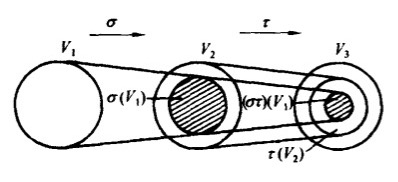
\includegraphics[scale=.5]{figs/6C.2.1.jpg}
          \end{figure}
          又因为 $ (\tau \sigma)(V_1) = \tau(\sigma(V_1)) $,所以又有
          \[ \dim(\tau \sigma)(V_1) \leqslant \dim \sigma(V_1) \]
          即 $ r(\tau \sigma) \leqslant r(\sigma) $.

          再证左边. 由线性映射维数公式,
          \begin{gather*}
              r(\tau) + \dim \ker \tau = n \\
              r(\tau \sigma) + \dim \ker(\tau \sigma) = m
          \end{gather*}
          又 $ \dim \ker(\tau \sigma) \leqslant \dim \ker \tau $,所以
          \[ m - r(\tau \sigma) = \dim \ker(\tau \sigma) \leqslant \dim \ker \tau \]
          代入线性映射维数公式,得 $ \dim \ker \tau = n - r(\tau) \geqslant m - r(\sigma) $,即
          \begin{align*}
              r(\tau \sigma) & \geqslant m + r(\tau) - n         \\
                             & \geqslant r(\sigma) + r(\tau) - n
          \end{align*}

    \item 证明:由于 $ \forall \beta \in (\sigma + \tau)(V_1),\enspace \exists \alpha \in V_1 $ 使 $ \beta = (\sigma + \tau)(\alpha) = \sigma(\alpha) + \tau(\alpha) \in \sigma(V_1) + \tau(V_1) $,所以
          \[ (\sigma + \tau)(V_1) \subseteq \sigma(V_1) + \tau(V_1) \]
          因此
          \begin{align*}
              \dim(\sigma + \tau)(V_1) & \leqslant \dim(\sigma(V_1) + \tau(V_1))     \\
                                       & \leqslant \dim \sigma(V_1) + \dim \tau(V_1)
          \end{align*}

    \item 证明:\begin{enumerate}
              \item \label{item:6:C:4:1}
                    $ \forall \sigma \in \mathcal{L}(V, V) $,则 $ I - \sigma \in \mathcal{L}(V, V) $. $ \forall \alpha \in (I - \sigma)(V),\enspace \exists \beta \in V $,有
                    \begin{gather*}
                        \alpha = (I - \sigma)(\beta) = \beta - \sigma(\beta) \\
                        \sigma(\alpha) = \sigma(\beta - \sigma(\beta)) = \sigma(\beta) - \sigma^2(\beta)
                    \end{gather*}
                    而由于 $ \sigma^2 = \sigma $,所以 $ \sigma(\alpha) = \vec{0} $,于是 $ \alpha \in \ker \sigma $,因此 $ (I - \sigma)(V) \subseteq \ker \sigma $.

              \item 利用 $ r(\sigma + \tau) \leqslant r(\sigma) + r(\tau) $ 和 $ r(\sigma) + \dim \ker \sigma = n $,由 \ref*{item:6:C:4:1} 可得
                    \begin{equation} \label{eq:6:C:4:2:1}
                        r(I - \sigma) + r(\sigma) \leqslant n
                    \end{equation}
                    又因为
                    \begin{equation} \label{eq:6:C:4:2:2}
                        r(I - \sigma) + r(\sigma) \geqslant r(I - \sigma + \sigma) = r(I) = n
                    \end{equation}
                    于是由\autoref{eq:6:C:4:2:1} 和\autoref{eq:6:C:4:2:2} 即可得到 $ r(I - \sigma) + r(\sigma) = n $.
          \end{enumerate}

    \item 证明:\begin{enumerate}
              \item \label{item:6:C:5:1}
                    $ \forall \alpha \in \im \sigma,\enspace \exists \beta \in V $ 使得 $ \sigma(\beta) = \alpha $. 由 $ \sigma^2 = \theta $ 可得 $ \sigma(\alpha) = \sigma^2(\beta) = \vec{0} $,因此 $ \alpha \in \ker \sigma $,从而 $ \im \sigma \subseteq \ker \sigma $. 于是我们得到
                    \[ n = \dim \im \sigma + \dim \ker \sigma \geqslant 2 \dim \im \sigma \]
                    即 $ \dim \im \sigma \leqslant \dfrac{n}{2} $.

              \item 由 \ref*{item:6:C:5:1} 可知,方程组 $ AX = \vec{0} $ 的基础解系含有 $ n - r(A) = \dim \ker \sigma \geqslant \dfrac{n}{2} $ 个解向量,所以结论成立.
          \end{enumerate}

    \item 假设 $ \alpha_1, \alpha_2, \ldots, \alpha_n \in \mathbf{F} $ 是 $ \mathbf{F} $ 作为数域 $ \mathbf{K} $ 上的线性空间的一组基,$ \beta_1, \ldots, \beta_m \in \mathbf{E} $ 是 $ \mathbf{E} $ 作为数域 $ \mathbf{F} $ 上的线性空间的一组基,则现在对于任意的 $ \beta \in \mathbf{E} $,都存在 $ k_1, \ldots, k_m \in \mathbf{F} $ 使得 $ \beta = \displaystyle\sum_{i = 1}^{m} k_i \beta_i $.

          而对于每一个 $ k_i \in \mathbf{F},\enspace i = 1, 2, \ldots, m $,存在 $ l_{ij} \in \mathbf{K},\enspace j = 1, 2, \ldots, n $ 使得 $ k_i = \displaystyle\sum_{j = 1}^{n} l_{ij} a_j $. 于是
          \[ \beta = \sum_{i = 1}^{m} \sum_{j = 1}^{n} l_{ij} \alpha_j \beta_i \]
          这说明对任意的 $ \beta \in \mathbf{E} $,都可由
          \[ \alpha_1 \beta_1, \ldots, \alpha_1 \beta_m, \alpha_2 \beta_1, \ldots, \alpha_n \beta_m \]
          这 $ mn $ 个向量线性表出,其中线性表出的系数都属于最小的数域 $ \mathbf{K} $.

          同时,如果假设 $ l_{ij} \in \mathbf{K} $ 满足 $ \displaystyle\sum_{i = 1}^{m} \sum_{j = 1}^{n} l_{ij} \alpha_j \beta_i = 0 $,则
          \[ \sum_{i = 1}^{m} \left(\sum_{j = 1}^{n} l_{ij} \alpha_j\right) \beta_i = 0 \]
          利用 $ \beta_1, \ldots, \beta_m $ 的线性无关性可得 $ \displaystyle\sum_{j = 1}^{n} l_{ij} \alpha_j = 0 $,再结合 $ \alpha_1, \ldots, \alpha_n $ 线性无关可得 $ l_{ij} = 0 $,这就说明 $ \alpha_1 \beta_1, \ldots, \alpha_1 \beta_m, \alpha_2 \beta_1, \ldots, \alpha_n \beta_m $ 在数域 $ \mathbf{K} $ 是线性无关的.

          综上,$ \alpha_1 \beta_1, \ldots, \alpha_1 \beta_m, \alpha_2 \beta_1, \ldots, \alpha_n \beta_m $ 就是 $ \mathbf{E} $ 作为 $ \mathbf{K} $ 的线性空间的一组基,从而这个线性空间是 $ mn $ 维的.
\end{enumerate}

\clearpage

\chapter{矩阵运算基础}

上一节我们将前面逐步搭建的线性空间与线性映射的抽象转变为具象的表达——矩阵——这是我们上一节最后内容总结中提到的利用坐标映射同构到最简单的向量空间的优越性的体现. 从本讲起的三讲内容中,我们的目光都会聚焦于具象的矩阵,但我们的视角时常会结合线性映射同步进行. 本讲我们首先介绍矩阵的基本运算的定义(及其与线性映射的关联)、性质与基本技巧,之后我们会在此基础上从线性映射的秩出发定义矩阵的秩,得到第一个重要的矩阵标准形——相抵标准形. 最后我们会更进一步加强运算技巧,介绍一些在解题或者是实际应用中常用的矩阵运算技巧.

\section{矩阵乘法}

\subsection{矩阵乘法的定义与基本性质}

我们首先给出矩阵乘法的定义:
\begin{definition}{}{}
    设$A=(a_{ij})_{p\times m},B=(b_{ij})_{m\times n}$,我们定义$A$与$B$的乘积矩阵$C=AB=(c_{ij})_{p\times n}$是一个$p\times n$矩阵,其中它的第$i$行第$j$列元素为矩阵$A$的第$i$行与矩阵$B$的第$j$列对应位置元素相乘后求和的结果,即
    \[c_{ij}=a_{i1}b_{1j}+a_{i2}b_{2j}+\cdots+a_{im}b_{mj}\enspace(i=1,\ldots,p,\enspace j=1,\ldots,n).\]
\end{definition}

事实上,这一定义带给我们的感受与我们在上一讲定义矩阵加法和数乘时的直观不同,在我们初看这一定义时必然会产生一个疑惑:为什么矩阵乘法定义得如此复杂,为什么不定义成两个矩阵对应元素相乘就可以了呢?事实上,这是因为矩阵乘法的定义来源于线性映射的复合的矩阵表示. 教材124--125页的推导通过线性映射的复合运算定义了矩阵的乘法运算,由于篇幅的限制,我们这里不再将教材中已有的内容重复. 在此我们给出两个线性映射的角度来理解矩阵乘法:
\begin{enumerate}
    \item 回顾上一节中提到的旋转$\theta$角的线性映射对应的矩阵$M_{\theta}=\begin{pmatrix}
                  \cos\theta & -\sin\theta \\
                  \sin\theta & \cos\theta
              \end{pmatrix}$. 我们考虑先旋转$\theta_1$,然后旋转$\theta_2$对应的两个变换$\sigma_1,\sigma_2$的复合$\sigma_2\sigma_1$,实际上就是旋转$\theta_1+\theta_2$角度,其矩阵表示为$M_{\theta_1+\theta_2}$,而矩阵乘法
          \begin{align*}
              M_{\theta_2}M_{\theta_1}
               & =\begin{pmatrix}
                      \cos\theta_2 & -\sin\theta_2 \\
                      \sin\theta_2 & \cos\theta_2
                  \end{pmatrix}\begin{pmatrix}
                                   \cos\theta_1 & -\sin\theta_1 \\
                                   \sin\theta_1 & \cos\theta_1
                               \end{pmatrix}                                                              \\
               & =\begin{pmatrix}
                      \cos\theta_2\cos\theta_1-\sin\theta_2\sin\theta_1 & -\cos\theta_2\sin\theta_1-\sin\theta_2\cos\theta_1 \\
                      \sin\theta_2\cos\theta_1+\cos\theta_2\sin\theta_1 & -\sin\theta_2\sin\theta_1+\cos\theta_2\cos\theta_1
                  \end{pmatrix} \\
               & =\begin{pmatrix}
                      \cos(\theta_1+\theta_2) & -\sin(\theta_1+\theta_2) \\
                      \sin(\theta_1+\theta_2) & \cos(\theta_1+\theta_2)
                  \end{pmatrix}=M_{\theta_1+\theta_2},
          \end{align*}
          这表明矩阵乘法$M_{\theta_2}M_{\theta_1}$的结果确实与$\sigma_2\sigma_1$的矩阵表示$M_{\theta_1+\theta_2}$一致.

    \item 回顾线性映射的复合,若复合$\sigma_1\sigma_2$符合定义,则必须有$\sigma_2$的到达空间恰好是$\sigma_1$的出发空间,故两空间维数一致,那么$\sigma_1$对应的矩阵$A$的列数和$\sigma_2$对应的矩阵$B$的行数一致,这也是我们要求两个矩阵$A,B$可乘的重要条件的来源. 而最后乘法的结果行数等于$A$的行数,列数等于$B$的列数,这也与$\sigma_1\sigma_2$出发空间为$\sigma_2$出发空间(对应于$B$的列数),到达空间为$\sigma_1$到达空间(对应于$A$的行数)一致.
\end{enumerate}

\begin{example}{}{}
    设$A=\begin{pmatrix}
            1 & 0 & -1 \\
            1 & 1 & -3
        \end{pmatrix}, B=\begin{pmatrix}
            0 & 3 \\
            1 & 2 \\
            3 & 1
        \end{pmatrix}$,求$AB$和$BA$.
\end{example}

\begin{solution}
    见教材126页例1.
\end{solution}

教材125页下方也介绍了几个矩阵运算的基本性质:
\begin{enumerate}
    \item $(AB)C=A(BC)$(结合律)

    \item $\lambda(AB)=(\lambda A)B=A(\lambda B),\enspace \lambda \in \mathbf{F}$

    \item $A(B+C)=AB+AC$(左分配律)

    \item $(B+C)P=BP+CP$(右分配律)
\end{enumerate}
证明方法十分简单暴力:直接设出矩阵元素然后暴力计算证明等号两边对应位置(如第$i$行第$j$列元素)相等即可. 125页下方给出了结合律的证明,感兴趣的同学可以参考,实际上记住结论即可.

实际上,由矩阵加法和乘法满足的运算律可知,全体$n$阶方阵构成的集合$\mathbf{F}^{n\times n}$关于矩阵加法和乘法构成环.

在本节最后,我们有四个非常重要的问题需要仔细探讨:
\begin{enumerate}
    \item 在有了矩阵乘法的定义后,高斯消元法中我们将线性方程组简记为$AX=b$实际上是相当自然的,除此之外,我们将向量坐标表示为列向量的形式,例如
          \[\vec{\alpha}=(\alpha_1,\alpha_2,\ldots,\alpha_n)\begin{pmatrix}
                  x_1 \\ x_2 \\ \vdots \\ x_n
              \end{pmatrix}\]
          这也是符合矩阵乘法定义的一种习惯(虽然基一般不是数域$\mathbf{F}$中的元素).

    \item 事实上,在这里我们可以看出求解线性方程组和线性映射之间的关联. 我们设$AX=b$的解为
          \[X=\begin{pmatrix}
                  x_1 \\ x_2 \\ \vdots \\ x_n
              \end{pmatrix}\]
          由$AX=b$和线性映射矩阵表示,我们有
          \begin{equation}\label{eq:7:方程组与核空间1}
              (\sigma(\varepsilon_1),\sigma(\varepsilon_2),\ldots,\sigma(\varepsilon_n))\begin{pmatrix}
                  x_1 \\ x_2 \\ \vdots \\ x_n
              \end{pmatrix}=(\alpha_1,\alpha_2,\ldots,\alpha_m)A\begin{pmatrix}
                  x_1 \\ x_2 \\ \vdots \\ x_n
              \end{pmatrix}=b
          \end{equation}
          即$x_1\sigma(\varepsilon_1)+x_2\sigma(\varepsilon_2)+\cdots+x_n\sigma(\varepsilon_n)=b$,即
          \begin{equation}\label{eq:7:方程组与核空间2}
              \sigma(x_1\varepsilon_1+x_2\varepsilon_2+\cdots+x_n\varepsilon_n)=b.
          \end{equation}
          由此我们将线性方程组的求解问题和找到线性映射到达空间中某个向量在出发空间中原像的坐标联系起来了,即将求解$AX=b$和求解$\sigma(a)=b$联系起来了,只是我们求解后者后还需要求出$a$在矩阵表示基下的坐标.

          若前述$b=0$,则我们将齐次线性方程组的解空间与线性映射的核空间联系起来了,即线性映射的核空间中元素在一组基下的向量就是这一线性映射在这组基下的矩阵表示作为系数矩阵的线性方程组的解. 这一联系将在\nameref{chap:朝花夕拾}中有更深入的讨论.

    \item 我们可以更进一步理解矩阵乘法. 假设矩阵$A=(a_{ij})_{m\times n}$与$B=(b_{ij})_{n\times l}$相乘,我们有如下结论:
          \begin{enumerate}
              \item 乘积的第$k$列等于$A$乘以$B$的第$k$列,乘积的第$j$行等于$A$的第$j$行乘以$B$,这一点根据矩阵乘法计算方式显然,我们可以利用这一性质证明下面例子的结论:
                    \begin{example}{}{}
                        设$A,B$都是由非负实数组成的矩阵且$AB$有一行等于0,证明:或者$A$有一行为0,或者$B$有一行为0.
                    \end{example}
                    \begin{proof}
                        设$A=(a_{ij})_{m\times n}$,$B=(b_{ij})_{n\times l}$,且设$AB=(c_{ij})_{m\times l}$的第$i$行为0,则根据前面的讨论可知就是$A$的第$i$行乘以$B$得到了全0行向量. 因此若$A$的第$i$行为0,则结论成立;否则$A$的第$i$行中存在某个元素大于0,不妨设$a_{ik}>0$,则此时$B$的第$k$行各元素必须均为0,否则若$b_{kj}>0$,我们有
                        \[c_{ij}=a_{i1}b_{1j}+\cdots+a_{ik}b_{kj}+\cdots+a_{in}b_{nj}>0,\]
                        综上可知结论成立.
                    \end{proof}

              \item 乘积的每一列都是矩阵$A$各列的线性组合,每一行都是矩阵$B$各行的线性组合. 我们简要说明前者,后者理由类似. 我们考察乘积的每一列,由1可知乘积的第$k$列等于$A$乘以$B$的第$k$列,我们展开写乘积矩阵$C=(c_{ij})_{m\times l}$第$k$列的结果:
                    \begin{align*}
                        c_{1k} & =a_{11}b_{1k}+a_{12}b_{2k}+\cdots+a_{1n}b_{nk} \\
                        c_{2k} & =a_{21}b_{1k}+a_{22}b_{2k}+\cdots+a_{2n}b_{nk} \\
                               & \vdotswithin{=}                                \\
                        c_{mk} & =a_{m1}b_{1k}+a_{m2}b_{2k}+\cdots+a_{mn}b_{nk}
                    \end{align*}
                    我们将上面的行进行组合,写成列向量形式,即
                    \[\begin{pmatrix}
                            c_{1k} \\ c_{2k} \\ \vdots \\ c_{mk}
                        \end{pmatrix}=b_{1k}\begin{pmatrix}
                            a_{11} \\ a_{21} \\ \vdots \\ a_{m1}
                        \end{pmatrix}+b_{2k}\begin{pmatrix}
                            a_{12} \\ a_{22} \\ \vdots \\ a_{m2}
                        \end{pmatrix}+\cdots+b_{nk}\begin{pmatrix}
                            a_{1n} \\ a_{2n} \\ \vdots \\ a_{mn}
                        \end{pmatrix}\]
                    由此我们将乘积的列表示成了矩阵$A$各列的线性组合.
          \end{enumerate}

    \item 之后我们会经常看见两种记号,即
          \begin{align*}
              (\sigma(\varepsilon_1),\sigma(\varepsilon_2),\ldots,\sigma(\varepsilon_n)) & =(\alpha_1,\alpha_2,\ldots,\alpha_m)A \\
              \sigma(\varepsilon_1,\varepsilon_2,\ldots,\varepsilon_n)                   & =(\alpha_1,\alpha_2,\ldots,\alpha_m)A
          \end{align*}
          教材中两个记号是等价的,这只是记号上的差别,含义完全相同. 但是在之后我们还会看到一个很特别的书写方式
          \[(\sigma(\varepsilon_1,\varepsilon_2,\ldots,\varepsilon_n))B=\sigma((\varepsilon_1,\varepsilon_2,\ldots,\varepsilon_n)B)\]
          教材不加解释地使用了这一等式,这容易导致读者的困惑,因此我们这里简要说明它们的确是等价的,从而接下来读者可以放心地自由使用这一结论.

          根据上述的第一个性质可知,我们只需要证明对$B$的某一列上式成立即可,因为乘法结果是列与列对应的. 我们设$B$的第$k$列为
          \[B_k=\begin{pmatrix}
                  b_{1k} \\ b_{2k} \\ \vdots \\ b_{nk}
              \end{pmatrix}\]
          则
          \begin{align*}
              (\sigma(\varepsilon_1,\varepsilon_2,\ldots,\varepsilon_n))
              \begin{pmatrix}
                  b_{1k} \\ b_{2k} \\ \vdots \\ b_{nk}
              \end{pmatrix}
               & =(\sigma(\varepsilon_1),\sigma(\varepsilon_2),\ldots,\sigma(\varepsilon_n))\begin{pmatrix}
                                                                                                b_{1k} \\ b_{2k} \\ \vdots \\ b_{nk}
                                                                                            \end{pmatrix} \\
               & =b_{1k}\sigma(\varepsilon_1)+b_{2k}\sigma(\varepsilon_2)+\cdots+b_{nk}\sigma(\varepsilon_n)                    \\
               & =\sigma(b_{1k}\varepsilon_1+b_{2k}\varepsilon_2+\cdots+b_{nk}\varepsilon_n)                                    \\
               & =\sigma((\varepsilon_1,\varepsilon_2,\ldots,\varepsilon_n)
              \begin{pmatrix}
                  b_{1k} \\ b_{2k} \\ \vdots \\ b_{nk}
              \end{pmatrix})
          \end{align*}
          故得证.
\end{enumerate}

事实上矩阵乘法有很多和数的乘法重要的不同,我们在此特别指出供读者参考:
\begin{enumerate}[label=(\arabic*)]
    \item 矩阵乘法不一定满足交换律(即$AB$不一定等于$BA$,事实上随手写两个矩阵,很大的概率就是不交换的,甚至交换过来不可乘). 因此实数的完全平方公式代入矩阵不一定成立,即很多时候$(A+B)^2=A^2+AB+BA+B^2\neq A^2+2AB+B^2$;

    \item 但是注意数量矩阵(即对角线上元素都相等,其余均为0,单位矩阵是其特例)和任何矩阵相乘都是可交换的,这一点在矩阵求幂时很有用;

    \item \label{item:7:矩阵乘法:3}
          $A\neq O$且$B\neq O$不能推出$AB\neq O$. 例如线性方程组$AX = 0$有非零解,若$B$的各列均为方程非零解,则$AB = O$.

    \item 消去律也不一定满足:即$AB = AC$不一定$A = B$. 原因在于$AB=AC \implies A(B-C)=O$,由 \ref*{item:7:矩阵乘法:3} 可知不一定$B = C$.
\end{enumerate}

\subsection{矩阵多项式}

我们在线性空间中已经介绍过,我们一般用$\mathbf{F}[x]_{m+1}$表示数域$\mathbf{F}$上的次数最高为$m$的多项式全体,其中的元素我们一般记为
\[p(x)=a_mx^m+a_{m-1}x^{m-1}+\cdots+a_1x+a_0,\enspace a_i\in\mathbf{F}\enspace(i=1,2,\ldots,m)\]
事实上这里的自变量不一定需要是一个数,也可以是线性映射或者矩阵. 例如线性映射$\sigma:V\to V$构成的$m$次多项式可以记为
\[p(\sigma)=a_m\sigma^m+a_{m-1}\sigma^{m-1}+\cdots+a_1\sigma+a_0I\]
其中$\sigma^i$表示$\sigma$复合$i$次,$I$表示恒等映射. 我们很容易说明当$\sigma$在$V$的一组基下矩阵表示为$A$时,$p(\sigma)$在同一组基下的矩阵表示为
\[p(A)=a_mA^m+a_{m-1}A^{m-1}+\cdots+a_1A+a_0E,\]
其中$E$表示单位矩阵. 由此我们便得到了矩阵多项式的定义,我们有如下几点需要强调:
\begin{enumerate}
    \item 这里我们要求$\sigma$是线性变换(即出发空间和到达空间一致),事实上也并不必要,只需出发空间和到达空间维数相同即可,因为我们的目的是保证矩阵的幂次可以定义(即$A$和$A$可乘,因此$A$的行列数一致);

    \item 上面的定义隐含:$\sigma^0 = I$,$A^0=E$;

    \item $A^kA^m=A^{k+m},\enspace (A^k)^m=A^{km}$,其中$A$为方阵,$k,m$为任意整数. 负整数对应于逆矩阵的情况,接下来可逆的部分会作进一步解释.
\end{enumerate}

\begin{example}{}{}
    展开矩阵多项式$(A+\lambda E)^n$.
\end{example}

\begin{solution}
    由于$A$与$E$是可交换的,并且$A^nE^m=A^n$显然成立,因此我们结合中学学过的二项式展开,得到结果:
    \begin{align*}
        (A+\lambda E)^n & =\sum_{i=0}^nC_n^iA^i(\lambda E)^{n-i}    \\
                        & =\sum_{i=0}^nC_n^i\lambda^{n-i}A^iE^{n-i} \\
                        & =\sum_{i=0}^nC_n^i\lambda^{n-i}A^i.
    \end{align*}
\end{solution}

\begin{example}{}{矩阵多项式可交换}
    设$f(x),g(x) \in \mathbf{F}[x],\enspace A,B \in \mathbf{M}_n(\mathbf{F})$. 证明:
    \begin{enumerate}
        \item $f(A)g(A)=g(A)f(A)$;

        \item 如果$AB=BA$,则$f(A)g(B)=g(B)f(A)$;
    \end{enumerate}
\end{example}

\begin{solution}
    我们可以直接证明第二点,因为第一点是第二点的特例. 设$f(x)=\displaystyle\sum_{i=0}^ma_ix^i$,$g(x)=\displaystyle\sum_{j=0}^sb_jx^j$,$A^0=B^0=E$,则
    \begin{align*}
        f(A)g(B) & =\sum_{i=0}^ma_iA^i\cdot \sum_{j=0}^sb_jB^j(AB=BA)                                 \\
                 & =\sum_{k=0}^{m+s}\sum_{i+j=k}a_ib_jA^iB^j=\sum_{k=0}^{m+s}\sum_{i+j=k}b_ja_iB^jA^i \\
                 & =g(B)f(A).
    \end{align*}
    事实上由于$A\cdot A=A\cdot A$,因此$f(A)g(A)=g(A)f(A)$只是上面证明的结论的特例.
\end{solution}

\section{一组例题}

在介绍了矩阵乘法后,我们可以进一步审视线性映射矩阵表示的定义. 我们来看一组初学时可能混淆或者不理解的例子,从而加深对概念的理解:
\begin{example}{}{矩阵表示2}
    设$A=\begin{pmatrix}1 & 0 & 2 \\ -1 & 2 & 1 \\ 1 & 2 & 5\end{pmatrix}$为两个三维线性空间之间的线性映射$\sigma$对应的矩阵,求$\sigma$的像空间和核空间.
\end{example}
(注:本题没有给出线性映射出发空间和到达空间的基,读者可以任意假设.)

\begin{solution}
    求解像空间和核空间,仍然是原先介绍的方法,虽然本题没有给出线性映射的直接定义,但矩阵表示也能给我们足够的信息. 我们设这一矩阵表示的线性映射为$\sigma$,且
    \[(\sigma(\varepsilon_1),\sigma(\varepsilon_2),\sigma(\varepsilon_3))=(\alpha_1,\alpha_2,\alpha_3)A\]
    根据线性映射矩阵表示的定义,我们知道矩阵表示就是线性映射在出发空间一组基下的像在到达空间一组基下的坐标按列排列,因此
    \begin{align*}
        \sigma(\varepsilon_1) & =\alpha_1-\alpha_2+\alpha_3   \\
        \sigma(\varepsilon_2) & =2\alpha_2+2\alpha_3          \\
        \sigma(\varepsilon_3) & =2\alpha_1+\alpha_2+5\alpha_3
    \end{align*}
    因此$\im\sigma=\spa(\alpha_1-\alpha_2+\alpha_3,2\alpha_2+2\alpha_3,2\alpha_1+\alpha_2+5\alpha_3)$,然后求解极大线性无关组即可,结果为$\im\sigma=\spa(\alpha_1-\alpha_2+\alpha_3,2\alpha_2+2\alpha_3)$

    这里求解极大线性无关组的方法我们可以回忆\autoref{ex:转化为坐标},我们先将三个向量转化为到达空间基下坐标,然后求解极大线性无关组,最后把基添加回来即可. 实际上我们会发现,这里的三个坐标就是矩阵$A$的三个列向量(因为矩阵表示就是线性映射在出发空间一组基下的像在到达空间一组基下的坐标按列排列),因此我们只需要求解矩阵$A$的列向量的极大线性无关组$(1,-1,1),(0,2,2)$,然后再将到达空间的基添加回来即可.

    然后求解核空间,我们设$\sigma(\varepsilon)=0$,将$\varepsilon$写成出发空间基的表示后事实上就是\autoref{eq:7:方程组与核空间2} 的形式,我们已说明这一形式与\autoref{eq:7:方程组与核空间1} 等价,因此我们只需求解$AX=0$然后代回出发空间的基即可,最终结果为$\ker\sigma=\spa(4\varepsilon_1+3\varepsilon_2-2\varepsilon_3)$.
\end{solution}

总结一下,此类题目求解像空间实际上就是求出矩阵列向量的极大线性无关组,然后记得把基添加回来. 求解核空间只需求解齐次线性方程组$AX=0$即可.

\begin{example}{}{矩阵表示3}
    已知3阶矩阵$A=\begin{pmatrix}
            1 & 0 & 1 \\ 0 & -1 & 0 \\ -1 & 1 & -1
        \end{pmatrix}$. 定义$\mathbf{R}^{3 \times 3}$上的线性变换$\sigma(X)=AX,\enspace X \in \mathbf{R}^{3 \times 3}$. 求$\sigma$的像和核.
\end{example}

\begin{solution}
    核空间求解较为简单,我们先求解核空间. 我们首先求解线性方程组$AY=0$,其中$Y$为列向量,解得其基础解系为$\eta=(1,0,-1)^\mathrm{T}$.

    记$X=(X_1,X_2,X_3)$,则$X\in\ker\sigma$即$AX=(AX_1,AX_2,AX_3)=O$,即$AX_1=AX_2=AX_3=0$,因此$X_1,X_2,X_3$都能由$\eta$线性表出,故
    \[X=(k_1\eta,k_2\eta,k_3\eta)=\begin{pmatrix}
            k_1 & k_2 & k_3 \\ 0 & 0 & 0 \\ -k_1 & -k_2 & -k_3
        \end{pmatrix},\enspace k_1,k_2,k_3\in\mathbf{R},\]
    即$X=k_1\begin{pmatrix}
            1 & 0 & 0 \\ 0 & 0 & 0 \\ -1 & 0 & 0
        \end{pmatrix}+k_2\begin{pmatrix}
            0 & 1 & 0 \\ 0 & 0 & 0 \\ 0 & -1 & 0
        \end{pmatrix}+k_3\begin{pmatrix}
            0 & 0 & 1 \\ 0 & 0 & 0 \\ 0 & 0 & -1
        \end{pmatrix}$,即$\ker\sigma$中所有元素均可由这三个矩阵线性表示,并且这三个矩阵显然线性无关,因此核空间就是这三个矩阵的线性组合,且核空间维数为3.

    注意到$\mathbf{R}^{3 \times 3}$的一组基为$E_{11},E_{12},E_{13},E_{21},E_{22},E_{23},E_{31},E_{32},E_{33}$,其中$E_{ij}$表示第$i$行第$j$列元素为1,其余元素为0的矩阵,例如$E_{23}=\begin{pmatrix}
            0 & 0 & 0 \\ 0 & 0 & 1 \\ 0 & 0 & 0
        \end{pmatrix}$.

    根据$\sigma$的定义我们可以求得$\sigma(E_{11})=\sigma(E_{31})=\begin{pmatrix}
            1 & 0 & 0 \\ 0 & 0 & 0 \\ -1 & 0 & 0
        \end{pmatrix},\enspace \sigma(E_{12})=\sigma(E_{32})=\begin{pmatrix}
            0 & 1 & 0 \\ 0 & 0 & 0 \\ 0 & -1 & 0
        \end{pmatrix},\enspace \sigma(E_{13})=\sigma(E_{33})=\begin{pmatrix}
            0 & 0 & 1 \\ 0 & 0 & 0 \\ 0 & 0 & -1
        \end{pmatrix},\sigma(E_{21})=\begin{pmatrix}
            0 & 0 & 0 \\ -1 & 0 & 0 \\ 1 & 0 & 0
        \end{pmatrix},\enspace \sigma(E_{22})=\begin{pmatrix}
            0 & 0 & 0 \\ 0 & -1 & 0 \\ 0 & 1 & 0
        \end{pmatrix},\enspace \sigma(E_{23})=\begin{pmatrix}
            0 & 0 & 0 \\ 0 & 0 & -1 \\ 0 & 0 & 1
        \end{pmatrix}$. 所以$\sigma$的像空间为上述六个矩阵线性扩张而成的空间,即$\im\sigma=\spa(\sigma(E_{11}),\sigma(E_{12}),\sigma(E_{13}),\sigma(E_{21}),\sigma(E_{22}),\sigma(E_{23}))$. 又由\nameref{thm:线性映射基本定理}可知,$\dim\im\sigma=n-\dim\ker\sigma=6$,因此像空间就是这六个矩阵线性扩张而成的空间.
\end{solution}

实际上,\autoref{ex:矩阵表示2} 和\autoref{ex:矩阵表示3} 都属于已知映射求像和核的题目,求解方法仍然是原先介绍的方法,只是\autoref*{ex:矩阵表示2} 没有像\autoref{ex:矩阵表示1} 或\autoref*{ex:矩阵表示3} 给出了线性映射的定义,而是给出矩阵表示,但这也完全不影响我们的求解.

\section{矩阵的逆}

\subsection{可逆的基本概念}

要引入矩阵的逆的概念,我们需要首先讨论线性映射的逆. 我们这里给出线性映射的逆的定义:
\begin{definition}{线性映射的逆}{可逆映射} \index{ni@逆 (inverse)}
    设$\sigma \in \mathcal{L}(V_1,V_2)$. 若存在$\tau \in \mathcal{L}(V_2,V_1)$使得$\sigma \tau = I_{V_2}$且$\tau \sigma = I_{V_1}$,则称$\sigma$\term{可逆}\index{ni!ke@可逆 (invertible)},并称$\tau$为$\sigma$的逆映射\index{ni!yingshe@映射 (inverse map)}.
\end{definition}
其中$I_{V_1}$和$I_{V_2}$分别是$V_1$和$V_2$上的恒等映射.

在之前有关线性映射基本定理的讨论中,我们提到了双射的概念. 事实上,在映射的语境下,双射与可逆是完全等价的. 我们有如下定理:
\begin{theorem}{}{}
    设$\sigma \in \mathcal{L}(V_1,V_2)$,则$\sigma$可逆$\iff \sigma$是双射.
\end{theorem}

因此在本讲义的语境下,双射与可逆是完全等价的. 关于这一定理我们有如下说明:
\begin{enumerate}
    \item 定理证明不属于本讲义需要覆盖的内容,一般的微积分或数学分析教材都会涉及;

    \item 这一定理事实上不一定针对线性映射,对于函数而言也有双射与可逆等价,只是在函数的语境下逆映射被称为反函数;

    \item 由于双射要求单射和满射,而单射性与核空间维数为0等价,由线性映射基本定理,双射应有出发空间维数等于像空间维数,而满射性要求像空间维数等于到达空间维数,因此双射要求出发空间和到达空间必须维数相同.
\end{enumerate}

在\autoref{def:可逆映射} 的语境下,我们取$V_1$的一组基$B_1=\{\alpha_1,\alpha_2,\ldots,\alpha_n\}$,$V_2$的一组基$B_2=\{\beta_1,\beta_2,\ldots,\beta_n\}$(特别注意根据我们上述讨论两个空间维数一致),则$\sigma$关于$B_1$和$B_2$的矩阵为$A=(a_{ij})_{m \times n}$,$\tau$关于$B_2$和$B_1$的矩阵为$B=(b_{ij})_{n \times m}$.

我们知道线性映射的复合对应矩阵乘法,因此$\tau\sigma:V_1\to V_1$关于$V_1$的基$B_1$和$\sigma\tau:V_2\to V_2$关于$V_2$的基$B_2$对应的矩阵分别为$BA$和$AB$,而我们很容易证明恒等映射关于任何基的矩阵均为单位矩阵,因此我们有$BA=E$和$AB=E$. 由此我们从可逆映射的角度引入矩阵的逆的概念:
\begin{definition}{矩阵的逆}{}
    设$A \in \mathbf{M}_n(\mathbf{F})$. 若存在$B \in \mathbf{M}_n(\mathbf{F})$使得$AB=BA=E$,则称矩阵$A$可逆,并把$B$称为$A$的\term{逆矩阵}\index{ni!juzhen@矩阵 (inverse matrix)},记作 $ B = A^{-1} $.
\end{definition}
在一些比较经典的教材中可逆矩阵也被称为非奇异矩阵,不可逆矩阵被称为\term{奇异矩阵}\index{qiyijuzhen@奇异矩阵 (singular matrix)}.

注意,逆矩阵定义基于方阵,非方阵没有上述逆矩阵(具体原因将在未来讨论). 广义逆矩阵允许非方阵,但那是另一个定义,我们不需要掌握. 对于可逆矩阵,注意以下两个定理:
\begin{theorem}{}{}
    可逆矩阵$A$的逆矩阵唯一.
\end{theorem}

\begin{theorem}{}{}
    设$A,B\in \mathbf{M}_n(\mathbf{F})$,则$AB=E \iff A$与$B$互为逆矩阵(即对于方阵而言,$AB=E\iff BA=E\iff A,B$可逆).
\end{theorem}
这两个定理的证明见教材130页. 特别注意唯一性的证明,我们在证明群的单位元唯一时使用了完全一致的思想,请务必掌握.

\subsection{基本性质}

\begin{enumerate}[label=(\arabic*)]
    \item 主对角元都是非零数的对角矩阵一定可逆,且逆矩阵就是对角线上元素取倒数(单位矩阵即为特例,其逆矩阵是其自身);

    \item \label{item:8:逆矩阵性质:2}
          注意没有加法性质(例如$A$可逆(则$-A$也可逆),但$A+(-A)=O$不可逆),对于数乘有$(\lambda A)^{-1}=\lambda^{-1}A^{-1}$;

    \item \label{item:8:逆矩阵性质:3}
          $(AB)^{-1}=B^{-1}A^{-1},\enspace (A_1A_2\cdots A_k)^{-1}=A_k^{-1}\cdots A_2^{-1}A_1^{-1}$;注意这一点和 \ref*{item:8:逆矩阵性质:2} 的证明都只需要直接验证结果即可,即因为$ABB^{-1}A^{-1}=AA^{-1}=E$,所以根据逆的唯一性可知$(AB)^{-1}=B^{-1}A^{-1}$一定成立;

          注意,这种验证逆的相关性质思想(即直接验证相乘是否为单位矩阵,然后利用逆的唯一性的方法)在之后的讨论中也是非常常见的,希望读者掌握.

    \item $(A^k)^{-1}=(A^{-1})^k,\enspace A^kA^m=A^{k+m},\enspace (A^k)^m=A^{km}$;注意这里的$k$和$m$不一定需要非负,事实上负数就是逆矩阵的幂次或幂次的逆,如$A^{-2}=(A^{-1})^2=(A^2)^{-1}$;

    \item 若$A$和$B$可逆,则$A\neq O$且$B\neq O$能推出$AB\neq O$,并且$A$可逆且$AB=O$可以推出$B=O$. 除此之外还有消去律成立,即$A \neq O$则有$AB=AC \implies B=C$成立.
\end{enumerate}

需要强调的是,我们之后讨论运算性质的时候都是循着类似的思路,考虑加法、数乘、乘法(2个相乘,$n$个相乘,矩阵的幂)、逆、转置、共轭等,所以虽然每个地方给出的性质都很多,但实际上大致研究思路是一致的.

\subsection{逆矩阵的求解(基本方法I)}

在介绍完性质后我们非常关心如何给定一个具体的矩阵求出它的逆的问题,这里我们给出第一种基本方法,即基于解方程的方法.

事实上,我们在矩阵乘法一节中就将$AX=b$和$\sigma(a)=b$联系在一起,其中$\sigma$在某组基下表示矩阵为$A$. 回顾本讲开头引入可逆矩阵的过程,可逆矩阵$A$应当是可逆线性映射$\sigma$关于某组基的表示矩阵. 对于可逆映射而言,首先必须是单射,因此$\sigma(a)=b$只能有唯一解,因此$AX=b$只能有唯一解.

事实上我们可以很简便地表达出这个解. 我们在$AX=b$左右同时左乘$A^{-1}$(矩阵乘法不可交换所以必须在同一侧乘),有$A^{-1}AX=A^{-1}b$,即$X=A^{-1}b$.

因此,当$A$可逆时,对于任意的$b$线性方程组都有唯一解,且解可以被表示为$X=A^{-1}b$的形式. 因此我们可以通过解线性方程组的方法求解逆矩阵. 我们将通过下面这个例子详细介绍这种方法的计算过程:
\begin{example}{}{}
    用上述方法求矩阵$A=\begin{pmatrix}1 & -1 & 1 \\ 0 & 1 & 2 \\ 1 & 0 & 4\end{pmatrix}$的逆矩阵.
\end{example}

\begin{solution}
    见教材132页例3.
\end{solution}

关于逆矩阵的求解问题,我们将在介绍完初等变换后介绍第二种基本方法,剩余的进阶解法将在\nameref{chap:矩阵运算进阶}中介绍更多手段,以及我们会介绍矩阵方程求解的方法. 本节我们囿于一些计算技巧和基本概念暂未引入所以无法完全展开这些技巧.

\subsection{广义逆矩阵}

在本节开头我们提到,逆矩阵是基于方阵定义的. 对于非方阵而言,我们有如下广义逆的定义,当然不要求读者在这门课中掌握. 对于每一个$m \times n$阶矩阵$A$,都存在唯一的$n \times m$阶矩阵$X$,使得:
\begin{enumerate}
    \item $AXA=A$;

    \item $XAX=X$;

    \item $AX$和$XA$均为共轭对称矩阵.
\end{enumerate}
我们称$X$为矩阵$A$的Moore-Penrose广义逆矩阵,记作$X=A^\dagger$. 此处不赘述其证明和算法,感兴趣的同学可以自行查阅相关资料. 我们可以从两个角度认识这一定义,首先是取$A$为可逆矩阵,发现此定义是相容的,其次是通过这一矩阵可以获得线性方程组$AX=b$最小二乘解$X=A^\dagger b$. 广义逆矩阵在各个领域的研究中应用很广泛,所以在此提一下它的概念.

\section{矩阵的转置}
\subsection{基本定义与性质}

矩阵的转置也是一种非常基本的运算,事实上推进到现在这一概念应当已经不陌生了,我们首先给出矩阵转置的定义:

\begin{definition}{矩阵的转置}{}
    设$A=(a_{ij})_{m \times n}$,则$A$的\term{转置矩阵}\index{zhuanzhi@转置 (transpose)}是一个$n \times m$矩阵,记作$A^\mathrm{T}$,它的第$k$行正好是$A$的第$k$列($k=1,2,\ldots,n$);它的第$r$列正好是$A$的第$r$行($r=1,2,\ldots,m$).
\end{definition}

例如,设$A=\begin{pmatrix}1 & 2 & 3 & 4 \\ 5 & 6 & 7 & 8 \\ 9 & 10 & 11 & 12\end{pmatrix}$,则$A^\mathrm{T}=\begin{pmatrix}1 & 5 & 9 \\ 2 & 6 & 10 \\ 3 & 7 & 11 \\ 4 & 8 & 12\end{pmatrix}$.

下面的列举的矩阵转置的性质是基本且常用的:

\begin{enumerate}
    \item $(A^\mathrm{T})^\mathrm{T}=A$

    \item $(A+B)^\mathrm{T}=A^\mathrm{T}+B^\mathrm{T}$

    \item $(\lambda A)^\mathrm{T}=\lambda A^\mathrm{T},\enspace \lambda \in \mathbf{F}$

    \item $(AB)^\mathrm{T}=B^\mathrm{T}A^\mathrm{T},\enspace(A_1A_2\cdots A_n)^\mathrm{T}=A_n^\mathrm{T}\cdots A_2^\mathrm{T}A_1^\mathrm{T},\enspace(A^\mathrm{T})^m=(A^m)^\mathrm{T}$

    \item $(A^\mathrm{T})^{-1}=(A^{-1})^\mathrm{T}$
\end{enumerate}
关于上述性质我们有如下说明:
\begin{itemize}
    \item[1.] 从计算角度来看是显然的,简而言之就是矩阵第$i$行变成第$i$列后又变回了第$i$行,因此矩阵不变;

    \item[2--4.] 考虑从计算角度验证只需暴力计算即可,至于4的$n$个矩阵的情况只需要从两个相乘的情况出发数学归纳即可,最后的幂的性质实际上将$(A_1A_2\cdots A_n)^\mathrm{T}=A_n^\mathrm{T}\cdots A_2^\mathrm{T}A_1^\mathrm{T}$中的$A_i$全部取成$A$即可;

    \item[5.] 请不要忘记验证逆的运算性质的一般方法,我们只需要看到$(A^{-1})^\mathrm{T}A^\mathrm{T}=(AA^{-1})^\mathrm{T}=E$,这里第一个等号运用了上面第4点转置乘法的性质. 从这一式中我们看到$(A^{-1})^\mathrm{T}$是$A^\mathrm{T}$的逆矩阵,因此利用逆的唯一性即可得到$(A^\mathrm{T})^{-1}=(A^{-1})^\mathrm{T}$;
\end{itemize}

在熟悉了矩阵的基本运算性质后,我们可以来看下面这个例题进行综合练习:
\begin{example}{}{}
    已知矩阵 $A=\begin{pmatrix}a & b & c \\ d & e & f \\ h & x & y\end{pmatrix}$ 的逆是 $A^{-1}=\begin{pmatrix}-1 & -2 & -1 \\ 2 & 1 & 0 \\ 0 & -3 & -1\end{pmatrix}$,\\
    $B=\begin{pmatrix}a-2b & b-3c & -c \\ d-2e & e-3f & -f \\ h-2x & x-3y & -y\end{pmatrix}$. 求矩阵 $X$ 满足:

    \[X+\left(B(A^\mathrm{T}B^2)^{-1}A^\mathrm{T}\right)^{-1}=X\left(A^2(B^\mathrm{T}A)^{-1}B^\mathrm{T}\right)^{-1}(A+B)\]
\end{example}

\begin{solution}
    注意到
    \[B=A\begin{pmatrix}
            1 &  & \\ 2 & 1 & \\ & & 1
        \end{pmatrix} \begin{pmatrix}
            1 &  & \\ & 1 & \\ & -3 & 1
        \end{pmatrix} \begin{pmatrix}
            1 &  & \\ & 1 & \\ & & -1
        \end{pmatrix},\]
    从而 $B$ 由 $A$ 经过有限次初等变换得到,因 $A$ 可逆,故 $B$ 可逆. 一方面
    \[\textbf{LHS}=X+\left(B\left(A^{T} B^{2}\right)^{-1} A^{T}\right)^{-1}=X+B,\]
    另一方面
    \[\textbf{RHS}=X\left(A^{2}\left(B^{T} A\right)^{-1} B^{T}\right)^{-1}(A+B)=X A^{-1}(A+B),\]
    于是 $X=A=(A^{-1})^{-1}=\begin{pmatrix}
            -\frac{1}{3} & \frac{1}{3} & \frac{1}{3}  \\
            \frac{2}{3}  & \frac{1}{3} & -\frac{2}{3} \\
            -2           & -1          & 1
        \end{pmatrix}$.
\end{solution}

关于转置我们还有一个重要的例题需要读者掌握:
\begin{example}{}{转置求幂}
    设$\alpha=(1,-1,2)^\mathrm{T},\enspace\beta=(3,1,-2)^\mathrm{T},\enspace A=\alpha\beta^\mathrm{T}$,求$A^n$.
\end{example}

\begin{solution}
    由于$A^2=\alpha\beta^\mathrm{T}\alpha\beta^\mathrm{T}=\alpha(\beta^\mathrm{T}\alpha)\beta^\mathrm{T}=kA$,其中$k=\beta^\mathrm{T}\alpha=-2$,则$A^2=-2A$. 则可递推得到$A^n=(-2)^{n-1}A=(-2)^{n-1}\begin{pmatrix}
            3 & 1 & -2 \\ -3 & -1 & 2 \\ 6 & 2 & -4
        \end{pmatrix}$,原因在于$A^n$展开后中间会出现$n-1$个$\beta^\mathrm{T}\alpha$.
\end{solution}

事实上,在将来讲解矩阵运算技巧时我们还会大量运用本题的技巧,因此请读者务必重视本题. 除此之外,此前的所有矩阵运算我们都介绍了它们在线性映射中的对应,转置具备一定的特殊性,因为转置后的矩阵行列数交换,这意味着原先的线性映射出发空间和到达空间的维数交换,这使得对它的解读会更加复杂,我们需要以将来对偶空间的语言来讨论.

\subsection{对阵矩阵与反对称矩阵}

\begin{definition}{}{}
    设$A=(a_{ij})_{n \times n}$,如果$\forall i,j\in\{1,2,\ldots,n\}$均有$a_{ij}=a_{ji}$,则称$A$为对称矩阵. 若均有$a_{ij}=-a_{ji}$,则称$A$为反对称矩阵.
\end{definition}
由定义易知$A$为对称矩阵的充要条件为$A=A^\mathrm{T}$,$A$为反对称矩阵的充要条件为$A=-A^\mathrm{T}$.
\begin{example}{}{}
    证明以下几点性质:
    \begin{enumerate}
        \item 反对称矩阵主对角元均为0;

        \item $AA^\mathrm{T}$和$A^\mathrm{T}A$均为对称矩阵;

        \item 设$A,B$为$n$阶对称和反对称矩阵,则$AB+BA$是反对称矩阵;

        \item 对称矩阵的乘积不一定对称;

        \item 可逆的对称(反对称)矩阵的逆矩阵也是对称(反对称)矩阵.
    \end{enumerate}
\end{example}

\begin{solution}
    \begin{enumerate}
        \item 由于$A$为反对称矩阵,因此根据定义有$a_{ii}=-a_{ii}$,即$a_{ii}=0$;

        \item 由于$(AA^\mathrm{T})^\mathrm{T}=(A^\mathrm{T})^\mathrm{T}A^\mathrm{T}=AA^\mathrm{T}$,因此$AA^\mathrm{T}$为对称矩阵;同理可证$A^\mathrm{T}A$为对称矩阵;

        \item 由于$A,B$分别为对称和反对称矩阵,因此$(AB+BA)^\mathrm{T}=B^\mathrm{T}A^\mathrm{T}+A^\mathrm{T}B^\mathrm{T}=-AB-BA=-(AB+BA)$,因此$AB+BA$为反对称矩阵;

        \item 注意$(AB)^\mathrm{T}=B^\mathrm{T}A^\mathrm{T}=BA$,因为矩阵乘法不一定可交换,因此$AB$不一定对称;

        \item 因为$A$可逆有$(A^{-1})^\mathrm{T}=(A^\mathrm{T})^{-1}=A^{-1}$,因此$A^{-1}$为对称矩阵;同理可证$A$反对称的情况.
    \end{enumerate}
\end{solution}

事实上,关于对称矩阵和反对称矩阵的性质还有很多,我们将它们放在习题中供读者作为练习. 经过前面的讨论,我们已经看到转置和对称矩阵之间的关联,因此我们在之后在处理一些对称性很强的问题时,实际上都可以考虑利用转置来解决,例如:
\begin{example}{}{}
    $a,b,c,d$是四个实数. 证明$\begin{cases}
            a^2+b^2=1 \\
            c^2+d^2=1 \\
            ac+bd=0
        \end{cases}$成立的充分必要条件是$\begin{cases}
            a^2+c^2=1 \\
            b^2+d^2=1 \\
            ab+cd=0
        \end{cases}$.
\end{example}

\begin{solution}
    设$A=\begin{pmatrix}
            a & b \\ c & d
        \end{pmatrix}$,则有
    \[AA^\mathrm{T}=\begin{pmatrix}
            a^2+b^2 & ac+bd \\ ac+bd & c^2+d^2
        \end{pmatrix},\enspace A^\mathrm{T}A=\begin{pmatrix}
            a^2+c^2 & ab+cd \\ ab+cd & b^2+d^2
        \end{pmatrix}.\]
    因此题中的充要条件可以转化为$AA^\mathrm{T}=E$是$A^\mathrm{T}A=E$的充要条件. 这是显然的,因为$AA^\mathrm{T}=E\iff A^{-1}=A^\mathrm{T}\iff A^\mathrm{T}A=E$成立.
\end{solution}

\section{矩阵的共轭}

在将来的讨论中我们有时还会涉及到复矩阵的情况(即矩阵中元素为复数),因此我们需要引入矩阵的共轭的概念. 我们首先给出矩阵的共轭的定义(研究其对应的线性映射的意义不大,因此此处不介绍):
\begin{definition}{}{}
    设$A=(a_{ij})_{m \times n}$,则$A$的\term{共轭矩阵}\index{gongzhoujuzhen@共轭矩阵 (conjugate matrix)}为$\overline{A}=(\overline{a_{ij}})_{m \times n}$.
\end{definition}

由此可见,复矩阵的共轭就是对其中每个元素取了共轭. 我们可以很容易地验证共轭矩阵的运算性质:
\begin{enumerate}
    \item $\overline{A+B}=\overline{A}+\overline{B}$

    \item $\overline{\lambda A}=\overline{\lambda}\overline{A}$

    \item $\overline{AB}=\overline{A}\overline{B}$($n$个矩阵同理);$\overline{A^m}=\overline{A}^m$

    \item $\overline{A^\mathrm{T}}=(\overline{A})^\mathrm{T}$

    \item $\overline{A^{-1}}=\overline{A}^{-1}$
\end{enumerate}

\section{分块矩阵}

矩阵分块在矩阵计算中是非常核心的一种手段,这可以使得我们将大矩阵分为更容易处理的小矩阵,结合并行计算等工具能大大加速矩阵计算. 除此之外,基于分块矩阵的初等变换也是研究矩阵求逆、矩阵的秩以及矩阵分解等多个问题的重要工具.

\begin{definition}{}{}
    一般地,对于$m \times n$矩阵$A$,如果在行的方向分成$s$块,在列的方向分成$t$块,就得到$A$的一个$s \times t$\term{分块矩阵}\index{fenkuaijuzhen@分块矩阵 (block matrix)},记作$A=(A_{kl})_{s \times t}$,其中$A_{kl}\enspace(k=1,\ldots,s,\enspace l=1,\ldots,t)$称为$A$的子块.
\end{definition}
实际上上述表示方法就是将一般矩阵表示$A=(a_{ij})_{m \times n}$中的$a_{ij}$替换为了小块矩阵,字母含义并无变化,内层代表索引,外层代表总行列数(只是分块矩阵是块索引和块数). 我们接下来考察分块矩阵的运算性质.
\begin{enumerate}
    \item 分块矩阵的加法:设分块矩阵$A=(A_{kl})_{s \times t},\enspace B=(B_{kl})_{s \times t}$. 如果$A$与$B$对应的子块$A_{kl}$和$B_{kl}$都是同型矩阵,则
          \[A+B=(A_{kl}+B_{kl})_{s \times t}\]
          由此我们看到分块矩阵加法要求小块形状和行列分块数都一致,实际上回顾一般矩阵加法要求矩阵完全同型即可理解这一要求.

    \item 分块矩阵的数乘:设分块矩阵$A=(A_{kl})_{s \times t}$,$\lambda$是一个数,则
          \[\lambda A=(\lambda A_{kl})_{s \times t}\]
          实际上数乘最好理解,因为如此计算的效果相当于一般矩阵数乘的效果,即给每个元素都乘以一个常数$\lambda$.

    \item 分块矩阵的乘法:设$A=(a_{ij})_{m \times n},\enspace B=(b_{ij})_{n \times p}$,如果把$A,B$分别分块为$r \times s$和$s \times t$分块矩阵,且$A$的列分块法与$B$的行分块法相同(注意这些条件始终保证可乘性成立),则
          \[AB=\begin{pmatrix}
                  A_{11} & A_{12} & \cdots & A_{1s} \\
                  A_{21} & A_{22} & \cdots & A_{2s} \\
                  \vdots & \vdots & \ddots & \vdots \\
                  A_{r1} & A_{r2} & \cdots & A_{rs}
              \end{pmatrix}\begin{pmatrix}
                  B_{11} & B_{12} & \cdots & B_{1t} \\
                  B_{21} & B_{22} & \cdots & B_{2t} \\
                  \vdots & \vdots & \ddots & \vdots \\
                  B_{s1} & B_{s2} & \cdots & B_{st}
              \end{pmatrix}=C=(C_{kl})_{r \times t}\]
          其中$C$是$r \times t$分块矩阵,且$C_{kl}$与一般矩阵计算类似,即为$A$第$k$行块$B$的$l$列块对应元素相乘后相加,即
          \[C_{kl}=A_{k1}B_{1l}+A_{k2}B_{2l}+\cdots+A_{ks}B_{sl},\enspace k=1,\ldots,r,\enspace l=1,\ldots,t\]

    \item 分块矩阵的转置:大、小矩阵都要转置,这是分块矩阵与普通矩阵的一大性质差异;即$s \times t$分块矩阵$A=(A_{kl})_{s \times t}$转置后$A^\mathrm{T}=(B_{lk})_{t \times s}$为$t \times s$分块矩阵,且$B_{lk}=A_{kl}^\mathrm{T}$. 例如$\begin{pmatrix}
                  A_{11} & A_{12} \\ A_{21} & A_{22}
              \end{pmatrix}^\mathrm{T}=\begin{pmatrix}
                  A_{11}^\mathrm{T} & A_{21}^\mathrm{T} \\ A_{12}^\mathrm{T} & A_{22}^\mathrm{T}
              \end{pmatrix}$.

    \item 分块矩阵的共轭:事实上就是每个小分块都取共轭即可:
          \[\overline{A}=(\overline{A_{kl}})_{s \times t}\]
\end{enumerate}

补充以下注意事项:
\begin{enumerate}
    \item 常见的行列分块方法:将矩阵按行/列分块,注意$A(\beta_1,\ldots,\beta_n)=(A\beta_1,\ldots,A\beta_n)$成立,但当$A$在右侧时并不可乘,因为$\beta$是列向量,只有当$A$为行向量时才能使$\beta A$乘法是有意义的. 事实上按行分块也有对称的结论,即写成
          \[A=\begin{pmatrix}
                  A_1 \\ \vdots \\ A_s
              \end{pmatrix}\]
          时,我们有
          \[AB=\begin{pmatrix}
                  A_1B \\ \vdots \\ A_sB
              \end{pmatrix}.\]

    \item 分块矩阵求逆通常有两种方法,其一直接使用设未知数的方式完成,我们下面将给出例子,当然也可以利用后续介绍的分块矩阵初等变换进行解决:
          \begin{example}{}{}
              设$n$阶矩阵$A$分块为$A=\begin{pmatrix}
                      B & O \\ C & D
                  \end{pmatrix}$,其中$B,D$分别为$k$阶、$m$阶矩阵,求当$B,D$可逆时的$A^{-1}$.
          \end{example}

          \begin{solution}
              本题我们使用的方法非常直接,就是直接设出$A^{-1}$的形式,然后验证即可. 之后我们还会学习一种基于分块矩阵初等变换的进阶方法(事实上考试如果考察的话基本是本题的解法,分块矩阵初等变换是在教材中是小字部分). 设$A^{-1}=\begin{pmatrix}
                      X & Y \\ Z & T
                  \end{pmatrix}$,其中$X,T$分别为$k,m$阶矩阵,那么我们有
              \[\begin{pmatrix}
                      B & O \\ C & D
                  \end{pmatrix}\begin{pmatrix}
                      X & Y \\ Z & T
                  \end{pmatrix}=\begin{pmatrix}
                      BX & BY \\ CX+DZ & CY+DT
                  \end{pmatrix}=\begin{pmatrix}
                      E_k & O \\ O & E_m
                  \end{pmatrix},\]
              又由题意$A$可逆有$B,D$可逆,因此$BX=E_k$可得$X=B^{-1}$,$BY=O$可得$Y=O$,$CY+DT=DT=E_m$可得$T=D^{-1}$,$CX+DZ=CB^{-1}+DZ=O$可得$Z=-D^{-1}CB^{-1}$,因此
              \[A^{-1}=\begin{pmatrix}
                      B^{-1} & O \\ -D^{-1}CB^{-1} & D^{-1}
                  \end{pmatrix}.\]
          \end{solution}

    \item 分析分块矩阵与普通矩阵的运算性质的异同:
          \begin{enumerate}
              \item 分块矩阵转置需要注意大矩阵小分块都要转置;

              \item 分块矩阵每一块不一定是数,而是矩阵,因此小分块中出现$^{-1}$表示小分块求逆,但如果是一般矩阵就是矩阵元素直接求倒数即可;

              \item 分块矩阵加法乘法一定要保证块大小对应,否则不可加、不可乘;

              \item 其他很多性质都是将单个元素推广为一块,例如满足可加、可乘后的加法、乘法计算.
          \end{enumerate}
\end{enumerate}

\begin{example}{}{}
    设\[A=\begin{pmatrix}
            1 & 2 & 0  & 0  & 0  \\
            2 & 5 & 0  & 0  & 0  \\
            0 & 0 & -2 & 1  & 0  \\
            0 & 0 & 0  & -2 & 1  \\
            0 & 0 & 0  & 0  & -2
        \end{pmatrix},\enspace B=\begin{pmatrix}
            1  & 0 & 1 & 0 \\
            -1 & 2 & 3 & 0 \\
            1  & 2 & 0 & 4 \\
            0  & 1 & 2 & 4 \\
            0  & 0 & 1 & 4
        \end{pmatrix}\]
    利用分块矩阵的方法,求$A^2,\enspace AB,\enspace A^\mathrm{T},\enspace A^{-1}$.
\end{example}

\begin{solution}
    将$A$和$B$分别分块为
    \[A=\begin{pmatrix}
            A_1 & O \\ O & A_2
        \end{pmatrix},\enspace B=\begin{pmatrix}
            B_1 & B_2 \\ B_3 & B_4
        \end{pmatrix},\]
    其中$A_1=\begin{pmatrix}
            1 & 2 \\ 2 & 5
        \end{pmatrix},\enspace A_2=\begin{pmatrix}
            -2 & 1 & 0 \\ 0 & -2 & 1 \\ 0 & 0 & -2
        \end{pmatrix},\enspace B_1=\begin{pmatrix}
            1 & 0 \\ -1 & 2
        \end{pmatrix},\enspace B_2=\begin{pmatrix}
            1 & 0 \\ 3 & 0
        \end{pmatrix},\enspace B_3=\begin{pmatrix}
            1 & 2 \\ 0 & 1 \\ 0 & 0
        \end{pmatrix},\enspace B_4=\begin{pmatrix}
            0 & 4 \\ 2 & 4 \\ 1 & 4
        \end{pmatrix}$. 因此$A^2=\begin{pmatrix}
            A_1^2 & O \\ O & A_2^2
        \end{pmatrix},\enspace AB=\begin{pmatrix}
            A_1B_1 & A_1B_2 \\ A_2B_3 & A_2B_4
        \end{pmatrix},\enspace A^\mathrm{T}=\begin{pmatrix}
            A_1^\mathrm{T} & O \\ O & A_2^\mathrm{T}
        \end{pmatrix},\enspace A^{-1}=\begin{pmatrix}
            A_1^{-1} & O \\ O & A_2^{-1}
        \end{pmatrix}$. 上面的具体展开计算略过,我们这里只需要体会分块矩阵的运算性质即可.
\end{solution}

在这个例子中我们可以得到一个很关键的经验:分块对角矩阵求逆实际上就是对每一个分块求逆.

\vspace{2ex}
\centerline{\heiti \Large 内容总结}

本讲起我们介绍了矩阵的基本运算,我们不难发现,在引入矩阵后,我们一方面成功将线性方程组(矩阵表达的形式)解的本质理论的探究与之前所学习的线性空间、线性映射结合,从而迈出了里程碑式的一步;另一方面有形的矩阵表达也使得我们可以引入更多的计算技巧和工具,使我们未来的研究相对于前述章节而言更为具象.

我们首先通过线性映射的复合引入了矩阵乘法,介绍了矩阵乘法的性质(特别注意与数的乘法不同的点,例如不一定交换,不一定可消去等),介绍了矩阵多项式的计算——这与中学里学习的因式分解、二项式展开等较为相关. 当然介绍矩阵乘法时我们也说明了线性方程组如何用矩阵乘法表示,说明了矩阵乘法左乘和右乘与行、列线性组合的关联,也阐释了两个记号的统一性,这些都是希望读者能够理解的,因为一般教材对于这些内容都持``默认''态度,但实践中发现同学们存在较多问题,因此在此都进行了详细讲解. 接下来矩阵的逆我们从线性映射的逆引入,介绍了矩阵的逆的唯一性,以及一些基本性质,这些性质的证明都非常基本,读者应当熟练,为之后的矩阵运算进阶做准备. 逆矩阵的求解我们也介绍了一种基于线性方程组的方法,之后我们会介绍更常用的其它方法. 接下来矩阵的转置、共轭以及分块则显得更加简单,因为更加具象,当然之后在运算进阶中我们可能会看到更多高级的计算技巧,本节的内容仅仅是一个开始.

\vspace{2ex}
\centerline{\heiti \Large 习题}

\vspace{2ex}
{\kaishu 在数学的天地里,重要的不是我们知道什么,而是我们怎么知道什么.}
\begin{flushright}
    \kaishu
    ——毕达哥拉斯
\end{flushright}

\centerline{\heiti A组}
\begin{enumerate}
    \item 证明:若$AB=BA$,$AC=CA$,则$A,B,C$为同阶方阵,且
          \[A(BC)=(BC)A,\enspace A(B+C)=(B+C)A.\]

    \item $A,B$都是$n$阶矩阵,求下列等式成立的充分条件:
          \begin{enumerate}
              \item $(A+B)^3=A^3+3A^2B+3AB^2+B^3$;

              \item $(A+B)(A-B)=A^2-B^2$.
          \end{enumerate}

    \item 设$A$是$n$阶方阵且$A^n=O$,证明:
          \[(E_n-A)(E_n+A+A^2+\cdots+A^{n-1})=E_n.\]

    \item 证明:若线性映射$\sigma \in \mathcal{L}(V_1,V_2)$可逆,则其逆映射唯一.

    \item 证明:有一行元素或一列元素全为0的$n$阶方阵必定不可逆.

    \item 设$\alpha,\beta$为三维列向量,且$\alpha\beta^\mathrm{T}=\begin{pmatrix}
        -1 & 2  & 1  \\
        1  & -2 & -1 \\
        2  & -4 & -2
    \end{pmatrix}$,求$\alpha^\mathrm{T}\beta$.
\end{enumerate}

\centerline{\heiti B组}
\begin{enumerate}
    \item 若$f(x)$是$x$的实系数$m$次多项式:
          \[f(x)=a_mx^m+a_{m-1}x^{m-1}+\cdots+a_1x+a_0\]
          则有矩阵多项式:
          \[f(A)=a_mA^m+a_{m-1}A^{m-1}+\cdots+a_1A+a_0E\]
          其中 $A^0=E$.
          \begin{enumerate}
              \item 若$A$为对角矩阵$B=\begin{pmatrix}
                            \lambda_1 & 0 \\ 0 & \lambda_2
                        \end{pmatrix}$,证明:$f(A)=\begin{pmatrix}
                            f(\lambda_1) & 0 \\ 0 & f(\lambda_2)
                        \end{pmatrix}$;

              \item 若$A=P^{-1}BP$,证明:$f(A)=Pf(B)P^{-1}$.
          \end{enumerate}

    \item 设$A$为$n$阶可逆矩阵,$A$的每行各元素之和都等于$k$,证明:$k \neq 0$且$A^{-1}$的每行各元素之和都等于$\vphantom{\cfrac{1}{k}}\dfrac{1}{k}$.

    \item 已知矩阵$A=\begin{pmatrix}1 & 2 & a  \\
               1 & 3 & 0  \\
               2 & 7 & -a\end{pmatrix}$可以通过初等列变换转化为矩阵$B=\begin{pmatrix}1  & a & 2 \\
               0  & 1 & 1 \\
               -1 & 1 & 1\end{pmatrix}$.
          \begin{enumerate}
              \item 求常数$a$;

              \item 求满足$AP=B$的可逆矩阵$P$.
          \end{enumerate}

          \item 证明以下两个命题:
          \begin{enumerate}
              \item 证明:任一$n$阶方阵都可以表示为一个对称矩阵与一个反对称矩阵的和.
              \item 设$A$是$n$阶复矩阵,若$\overline{A}^\mathrm{T}=A$,则称$A$是一个Hermite矩阵. 若$\overline{A}^\mathrm{T}=-A$,则称$A$是一个斜Hermite矩阵. 证明:任一$n$阶复矩阵都可以表示为一个Hermite矩阵与一个斜Hermite矩阵的和.
          \end{enumerate}

    \item 证明以下两个命题:
          \begin{enumerate}
              \item 设$A$为$m\times n$阶实矩阵,则$A^\mathrm{T}A=O$的充要条件为$A=O$.
              \item 设$A$为$m\times n$阶复矩阵,则$\overline{A^\mathrm{T}}A=O$的充要条件为$A=O$.
          \end{enumerate}

    \item 证明以下两个命题:
          \begin{enumerate}
              \item 设$A$为$n$阶对称矩阵,证明:$A$是零矩阵的充要条件为对任意的$n$维向量$\alpha$,都有$\alpha^\mathrm{T}A\alpha=0$.
              \item 设$A$为$n$阶方阵,证明:$A$为反对称矩阵的充要条件为对任意的$n$维向量$\alpha$,都有$\alpha^\mathrm{T}A\alpha=0$.
          \end{enumerate}

    \item 证明:设$A$是实对称矩阵,若$A^2=O$,则$A=O$.

    \item 设$A,B$为$n$阶方阵,证明:
          \begin{enumerate}
              \item 若$A,B$为对称矩阵,则$AB$为对称矩阵的充要条件为$AB=BA$,$AB$为反对称矩阵的充要条件为$AB=-BA$.
              \item 若$A$为对称矩阵,$B$为反对称矩阵,则$AB$为反对称矩阵的充要条件为$AB=BA$,$AB$为对称矩阵的充要条件为$AB=-BA$.
          \end{enumerate}

    \item 求矩阵$\begin{pmatrix}
                  a  & b  & c  & d  \\
                  -b & a  & d  & -c \\
                  -c & -d & a  & b  \\
                  -d & c  & -b & a
              \end{pmatrix}$的逆.

    \item 设 $V=\{(a_{ij})_{n \times n} \mid \forall i,j,\enspace a_{ij}=a_{ji}\}$.
          \begin{enumerate}
              \item 证明:$V$为$\mathbf{F}^{n \times n}$的子空间;

              \item 求$V$的基和维数.
          \end{enumerate}

    \item $\mathbf{M}_n(\mathbf{R})$表示所有实$n$阶方阵构成的集合. 设$W=\{A\in \mathbf{M}_n(\mathbf{R}) \mid a_{ji}=ka_{ij},\enspace i \leqslant j\}$,求当$k=0,1,2$时,$W$的一组基和维数.
\end{enumerate}

\centerline{\heiti C组}
\begin{enumerate}
    \item 若$n$阶方阵$A_1,A_2,\ldots,A_m$满足$A_i^2\neq O\enspace(i=1,2,\ldots,m)$,且当$i\neq j$时$A_iA_j=O$,证明:$m\leqslant n$.

    \item 设 $A,B,C$ 为二阶复方阵,且 $A,B,C$ 在 $\mathbf{M}_2(\mathbf{C})$ 中线性无关. 证明:存在$z_1,z_2,z_3 \in \mathbf{C}$使得 $z_1A+z_2B+z_3C$ 为可逆矩阵.
\end{enumerate}

\chapter{相抵标准形}

推进到现在,我们已经将线性代数中几乎所有的基础知识学习完成,也就是说接下来的内容大都只是前面最基本内容的应用. 事实上,线性代数这门课有两大目标,其一是对线性空间进行分类,这是因为这一目标的实现也宣告了我们对线性空间这一代数结构基本已经研究清楚,此前我们在同构中已经完成了这一目标;第二个目标我们将从本讲开始探讨:我们希望求解线性映射在哪组基下的矩阵表示是简单的,本讲我们将给出这一问题的第一个重要答案,即相抵标准形.

本讲我们将分别从线性映射的角度和矩阵的角度推导相抵标准形的存在性,当然在此之前我们需要定义矩阵的秩作为基础. 线性映射的角度我们主要利用线性映射基本定理,矩阵的角度我们则定义了初等矩阵来辅助我们的工作. 最后我们将介绍相抵标准形的应用,这是基于相抵标准形的分解技巧,此类技巧在此后任意一种标准形的讨论中都是十分重要的.

\section{矩阵的秩}

我们首先给出矩阵的三个秩的定义:
\begin{definition}{}{}
    设$A$是线性映射$\sigma$对应的矩阵,我们把$\sigma$的秩也称为矩阵$A$的秩,记为$r(A)$,有时也简记为$r$. 我们将矩阵$A$的所有行向量组成的秩称为$A$的\term{行秩}\index{zhi!hang@行秩 (row rank)},常记为$r_r$. 所有列向量组成的向量组的秩称为$A$的\term{列秩}\index{zhi!lie@列秩 (column rank)},常记为$r_c$.
\end{definition}
对于以上定义的三个秩,我们有定理如下,这一定理无论是证明还是结果都非常关键:
\begin{theorem}{}{}
    任意矩阵$A=(a_{ij})_{m\times n}$的秩 = 行秩 = 列秩.
\end{theorem}
定理的证明我们分为两步:
\begin{enumerate}
    \item 证明矩阵的秩 = 列秩

          \begin{proof}
              设$\sigma:V_1\to V_2$,$A$是$\sigma$关于$V_1$和$V_2$的基$B_1=\{\alpha_1,\ldots,\alpha_n\}$和$B_2=\{\beta_1,\ldots,\beta_m\}$的矩阵. 由线性映射矩阵表示的定义可知,矩阵的列向量组就是向量组$S=\{\sigma(\alpha_1),\ldots,\sigma(\alpha_n)\}$在基$B_2$下的坐标按列排列.

              回忆坐标映射是同构映射,由\autoref{thm:同构保秩},$S$和$A$的列向量组秩相等. 又根据线性映射像空间的求解,$\dim\im\sigma=r(S)$,且根据矩阵的秩的定义$r(A)=\dim\im\sigma$,而$A$列向量组的秩也就是列秩$r_c$,因此我们有$r(A)=r_c$.
          \end{proof}

    \item 证明矩阵的行秩 = 列秩:行秩等于列秩有四样证法,你知道么?接下来我们先给出两种证明,在介绍相抵标准形后给出\hyperref[pf:11:矩阵行秩=列秩]{第三种证明},最后一种我们放在内积空间中介绍.
          \begin{enumerate}
              \item (证法一,《大学数学:代数与几何》证明方法)

                    \begin{proof}
                        设$A$的行秩为$r_r$,即$A$有$r_r$个线性无关的行向量,记为$\alpha_1,\ldots,\alpha_{r_r}$. 因此所有行向量都可以被这$r_r$个行向量线性表示,即
                        \[\alpha_i=\sum_{k=1}^{r_r}c_{ik}\alpha_k \qquad i=1,2,\ldots,m\]
                        我们将$\alpha_i$展开为行向量形式有
                        \[(a_{i1},\ldots,a_{in})=\sum_{k=1}^{r_r}(c_{ik}a_{k1},\ldots,c_{ik}a_{kn}) \qquad i=1,2,\ldots,m\]
                        故每一项可以写为$a_{ij}=\displaystyle\sum_{k=1}^{r_r}c_{ik}a_{kj},\enspace i=1,2,\ldots,m,\enspace j=1,2,\ldots,n$. 因此每一列可以写为
                        \[\begin{pmatrix}
                                a_{1j} \\ \vdots \\ a_{mj}
                            \end{pmatrix}=\sum_{k=1}^{r_r}a_{kj}\begin{pmatrix}
                                c_{1k} \\ \vdots \\ c_{mk}
                            \end{pmatrix} \qquad j=1,2,\ldots,n\]
                        上式表明$A$的所有列向量都可以被$r_r$个列向量$(c_{1k},\ldots,c_{mk})^\mathrm{T},\enspace k=1,2,\ldots,r_r$线性表示,因此$A$的列秩$r_c\leqslant r_r$.

                        由于上面的推导对任意矩阵都成立,我们考察$A$的转置$A^\mathrm{T}$,我们也可以得到$A^\mathrm{T}$的列秩小于等于$A^\mathrm{T}$的行秩,也就是$A$的行秩小于等于$A$的列秩,即$r_r\leqslant r_c$,因此我们有$r_r=r_c$.
                    \end{proof}

              \item (证法二,《线性代数应该这样学》证明方法,需要基于对偶映射)

                    \begin{proof}
                        设$A$是$\sigma:V\to W$在$V$和$W$一组基下的矩阵,由对偶映射矩阵表示可知,$A^\mathrm{T}$是$\sigma^*:W^*\to V^*$在$W^*$和$V^*$对偶基下的矩阵,故我们有:
                        \[A\text{~的列秩}=\dim\im\sigma=\dim\im\sigma^*=A^\mathrm{T}\text{~的列秩}=A\text{~的行秩}.\]
                        其中第1,3个等号来源于矩阵的秩=列秩,第2个等号来源于\autoref{thm:对偶映射像和核的性质}.
                    \end{proof}
          \end{enumerate}
\end{enumerate}

关于这一定理,我们有以下几点补充说明:
\begin{enumerate}
    \item 矩阵的秩等于列秩的证明我们复习了同构的性质. 事实上这一结论还可以告诉我们,无论是$\sigma$在哪组基下的表示矩阵,都有相同的秩;除此之外,这一定理使得我们可以将求矩阵的秩的问题转化为求矩阵行/列极大线性无关向量组的问题;

    \item 行秩等于列秩的第一种证明给了我们两个启示:
          \begin{enumerate}
              \item 我们在证明过程第二步证明反向不等式的时候直接考察了转置矩阵得出结论,这一思想在将来一些秩的等式/不等式的证明中也是常见的,因为转置就是将行和列互换,所以特别适合于这种证明;

              \item $r(A)=r(A^\mathrm{T})$,即矩阵转置不改变矩阵的秩. 事实上根据这一定理我们有$A^\mathrm{T}$的行秩=$A$的列秩=$A$的秩=$A$的行秩=$A^\mathrm{T}$的列秩=$A^\mathrm{T}$的秩.
          \end{enumerate}
          除此之外,我们可以仔细品味以下行秩=列秩这一结论. 这表明我们随手写任意一个矩阵,它行向量组的秩和列向量组的秩就一定是相等的——明明是很杂乱无章的数字排列,却有这么一个和谐而美观的性质,着实令人赞叹. 事实上,行秩=列秩还有更深层的含义等待我们在后续章节中逐步揭示,届时我们也将给读者一个比较完整的对矩阵转置的理解.
\end{enumerate}

除此之外,我们还应强调以下结论,在后续研究线性方程组解的性质时是常用的:
\begin{theorem}{}{单满射与行列秩}
    线性映射是单射当且仅当其矩阵表示为列满秩矩阵,线性映射是满射当且仅当其矩阵表示为行满秩矩阵.
\end{theorem}

\begin{proof}
    设$\sigma:V\to W$,其中$\dim V=n$,$\dim W=m$,且$\sigma$的矩阵表示为$A$,则$A$是$m\times n$矩阵.
    \begin{enumerate}
        \item $\sigma$是单射$\iff\dim\ker\sigma=0\iff \dim\im\sigma=\dim V-\dim\ker\sigma=n\iff r(A)=n\iff A$是列满秩矩阵;

        \item $\sigma$是满射$\iff\dim\im\sigma=m\iff r(A)=m\iff A$是行满秩矩阵.
    \end{enumerate}
    特别注意$A$是$m\times n$矩阵,因此上述两式的最后两个等价条件成立.
\end{proof}

我们需要注意,虽然之前证明矩阵的秩=列秩时我们将列秩和像空间的秩等同,但这里列满秩是和单射等同的,不要混淆. 事实上先证明出单射等价于列满秩,再利用\autoref{cor:对偶映射单满射} 可知满射等价于行满秩,因为综合可得$\sigma$是单射$\iff\sigma^*$是满射$\iff A$是列满秩矩阵$\iff A^\mathrm{T}$是行满秩矩阵,结合$A^\mathrm{T}$是$\sigma^*$的表示矩阵可知满射等价于行满秩.

事实上,通过矩阵的秩的学习我们还总结可逆矩阵的几个等价条件:
\begin{theorem}{}{可逆等价条件}
    设$A \in \mathbf{M}_n(\mathbf{F})$,则下列命题等价:
    \begin{enumerate}[label=(\arabic*)]
        \item \label{item:11:可逆等价条件:1}
              $A$可逆;

        \item \label{item:11:可逆等价条件:2}
              $r(A)=n$;

        \item \label{item:11:可逆等价条件:3}
              $A$的$n$个行(列)向量线性无关;

        \item \label{item:11:可逆等价条件:4}
              齐次线性方程组$AX=0$只有零解.
    \end{enumerate}
\end{theorem}

\begin{proof}
    相信读者在学习了未竟专题一,或者在学习数学分析或微积分等课程时已经了解了如何推导等价条件,即只需要找到一条逻辑循环链路即可.
    \begin{itemize}
        \item[\ref*{item:11:可逆等价条件:1}$\implies$\ref*{item:11:可逆等价条件:2}] $A$可逆我们有$A$对应的线性映射为可逆映射(既单又满),由\autoref{thm:单满射与行列秩} 可知$A$的行列秩都为$n$,即$r(A)=n$;

        \item[\ref*{item:11:可逆等价条件:2}$\implies$\ref*{item:11:可逆等价条件:3}] $r(A)=n$,则$A$的行列秩都为$n$,即$A$的$n$个行(列)向量线性无关;

        \item[\ref*{item:11:可逆等价条件:3}$\implies$\ref*{item:11:可逆等价条件:4}] 设$A$的$n$个列向量为$\beta_1,\ldots,\beta_n$,则$AX=0$等价于$x_1\beta_1+\cdots+x_n\beta_n=0$,由于$\beta_1,\ldots,\beta_n$线性无关,故$x_1=\cdots=x_n=0$,即$AX=0$只有零解;

        \item[\ref*{item:11:可逆等价条件:4}$\implies$\ref*{item:11:可逆等价条件:1}] 只有零解表示$A$经过初等行变换$P_1,\ldots,P_s$后得到了单位矩阵$E$,即
              \[P_s\cdots P_1A=E\]
              又初等矩阵可逆,则$A=(P_s\cdots P_1)^{-1}$,又由可逆矩阵的乘积仍然可逆,则$A$可逆.
    \end{itemize}
\end{proof}

事实上,在学完行列式后这一命题还可以增加一个行列式$|A|\neq 0$的等价条件.

\section{三个重要的定理}

这一讲我们将讨论三个容易混淆但各有十分重要内涵的定理. 其中第一个定理引入过渡矩阵且与矩阵的秩有较大关联,后面两个定理放在一起讨论是为了说明这三个看起来很类似的定理的本质区别. 在讨论第一个定理前我们首先介绍过渡矩阵(变换矩阵)的概念.
\begin{definition}{}{}
    设$B_1=\{\alpha_1,\alpha_2,\ldots,\alpha_n\}$与$B_2=\{\beta_1,\beta_2,\ldots,\beta_n\}$是线性空间$V(\mathbf{F})$的任意两组基,$B_2$中每个基向量被基$B_1$表示为
    \[ \begin{cases} \begin{aligned}
                \beta_1 & = a_{11}\alpha_1+a_{21}\alpha_2+\cdots+a_{n1}\alpha_n \\
                \beta_2 & = a_{12}\alpha_1+a_{22}\alpha_2+\cdots+a_{n2}\alpha_n \\
                        & \vdotswithin{=}                                       \\
                \beta_n & = a_{1n}\alpha_1+a_{2n}\alpha_2+\cdots+a_{nn}\alpha_n
            \end{aligned} \end{cases} \]
    将上式用矩阵表示为
    \[(\beta_1,\beta_2,\ldots,\beta_n)=(\alpha_1,\alpha_2,\ldots,\alpha_n)\begin{pmatrix}
            a_{11} & a_{12} & \cdots & a_{1n} \\
            a_{21} & a_{22} & \cdots & a_{2n} \\
            \vdots & \vdots & \ddots & \vdots \\
            a_{n1} & a_{n2} & \cdots & a_{nn}
        \end{pmatrix}\]
    我们将这一矩阵称为即$B_1$变为基$B_2$的变换矩阵(或过渡矩阵).
\end{definition}
简单而言$B_1$变为基$B_2$的过渡矩阵就是将$B_2$中的向量在$B_1$下的坐标按列排列. 关于这一定义,我们有以下几点需要强调:
\begin{enumerate}
    \item 在之后的讨论或者题目中需要特别注意说的是$B_1$变为基$B_2$的过渡矩阵还是反过来基$B_2$变为基$B_1$的过渡矩阵;

    \item 注意过渡矩阵一定是基与基之间的表示矩阵,一般的向量组之间不称过渡矩阵;

    \item 过渡矩阵一定是可逆矩阵,且$B_1$变为基$B_2$的过渡矩阵的逆矩阵就是$B_2$变为基$B_1$的过渡矩阵. 我们将首先介绍几个更一般的定理,然后这里的结论就会是显然的.
\end{enumerate}

\begin{theorem}{}{}
    设$\alpha_1,\alpha_2,\ldots,\alpha_n$是线性无关的向量组,且
    \[(\beta_1,\beta_2,\ldots,\beta_s)=(\alpha_1,\alpha_2,\ldots,\alpha_n)A\]
    则向量组$\beta_1,\beta_2,\ldots,\beta_s$的秩等于矩阵$A$的秩.
\end{theorem}

\begin{proof}
    由定义,$A$的各列是向量组$\beta_1,\beta_2,\ldots,\beta_s$在线性无关向量组$\alpha_1,\alpha_2,\ldots,\alpha_n$下的坐标. 我们知道向量和坐标之间存在坐标映射这一同构映射,故向量组$\beta_1,\beta_2,\ldots,\beta_s$的秩等于矩阵$A$的列秩,即$r(\beta_1,\beta_2,\ldots,\beta_s)=r(A)$.
\end{proof}

根据这一定理我们代入过渡矩阵的场景,此时线性无关向量组$\alpha_1,\alpha_2,\ldots,\alpha_n$是一组基,$\beta_1,\beta_2,\ldots,\beta_n$也是线性无关的一组基,因此$A$的秩等于$n$,即$A$行、列都满秩,对应的线性映射既满射又是单射,因此$A$可逆.
\begin{theorem}{}{}
    已知$\beta_i=a_{1i}\alpha_1+a_{2i}\alpha_2+\cdots+a_{ni}\alpha_n,\enspace i=1,2,\ldots,n$,且$A=(a_{ij})$可逆,则$\alpha_1,\alpha_2,\ldots,\alpha_n$与$\beta_1,\beta_2,\ldots,\beta_n$等价.
\end{theorem}

\begin{proof}
    由题意已经可知,向量组$\beta_1,\beta_2,\ldots,\beta_n$可以被向量组$\alpha_1,\alpha_2,\ldots,\alpha_n$线性表示,要证明两个向量组等价,我们只需反过来再证明向量组$\alpha_1,\alpha_2,\ldots,\alpha_n$可以被向量组$\beta_1,\beta_2,\ldots,\beta_n$线性表示即可. 由题意,
    \[(\beta_1,\beta_2,\ldots,\beta_n)=(\alpha_1,\alpha_2,\ldots,\alpha_n)A,\]
    由于$A$可逆,故$A^{-1}$存在,因此我们在上式等式两端同时乘以$A^{-1}$,即可得到
    \[(\alpha_1,\alpha_2,\ldots,\alpha_n)=(\beta_1,\beta_2,\ldots,\beta_n)A^{-1}.\]
    由此可知向量组$\alpha_1,\alpha_2,\ldots,\alpha_n$也可以被向量组$\beta_1,\beta_2,\ldots,\beta_n$线性表示,得证.
\end{proof}

很显然,这一证明的关键步骤也可以用来说明基$B_1$变为基$B_2$的过渡矩阵的逆矩阵是$B_2$变为基$B_1$的过渡矩阵,因为过渡矩阵可逆,我们只需要将上述定理中的$\alpha_i$和$\beta_i$分别替换为基向量组即可. 我们来看一个例子:
\begin{example}{}{}
    已知$\beta_1=\alpha_2+\alpha_3,\enspace\beta_2=\alpha_1+\alpha_3,\enspace\beta_3=\alpha_1+\alpha_2$,证明$\alpha_1,\alpha_2,\alpha_3$与$\beta_1,\beta_2,\beta_3$等价.
\end{example}

\begin{solution}
    事实上,$(\beta_1,\beta_2,\beta_3)=(\alpha_1,\alpha_2,\alpha_3)\begin{pmatrix}
            0 & 1 & 1 \\
            1 & 0 & 1 \\
            1 & 1 & 0
        \end{pmatrix}$,而$\begin{pmatrix}
            0 & 1 & 1 \\
            1 & 0 & 1 \\
            1 & 1 & 0
        \end{pmatrix}$可逆(可以由\autoref{thm:可逆等价条件}(3)(4)很容易验证),故$\alpha_1,\alpha_2,\alpha_3$与$\beta_1,\beta_2,\beta_3$等价.
\end{solution}

有了上述内容的铺垫,我们可以开始介绍本节三个重要定理中的第一个:
\begin{theorem}{基的选择对向量坐标的影响}{基的选择对向量坐标的影响}
    设线性空间$V$的两组基为$B_1$和$B_2$,且基$B_1$到$B_2$的变换矩阵(过渡矩阵)为$A$,如果$\xi \in V(\mathbf{F})$在$B_1$和$B_2$下的坐标分别为$X$和$Y$,则$Y=A^{-1}X$.
\end{theorem}
上述定理描述了\textbf{同一个向量在不同基下坐标之间的关系}. 证明是简单的:

\begin{proof}
    由题意,$\xi$在两组基下有如下两种坐标表示:
    \[\xi=(\alpha_1,\ldots,\alpha_n)X=(\beta_1,\ldots,\beta_n)Y.\]
    将过渡矩阵的条件$B_2=B_1A$,即$(\beta_1,\ldots,\beta_n)=(\alpha_1,\ldots,\alpha_n)A$代入上式可得:
    \[\xi=(\alpha_1,\ldots,\alpha_n)X=(\alpha_1,\ldots,\alpha_n)AY.\]
    又由于$\xi$在线性无关向量组$\alpha_1,\ldots,\alpha_n$下的坐标唯一,故我们有$X=AY$,即$Y=A^{-1}X$.
\end{proof}

接下来我们来看第二个重要的定理:
\begin{theorem}{线性映射对向量坐标的影响}{线性映射对向量坐标的影响}
    设$\sigma \in \mathcal{L}(V_1,V_2)$关于$V_1$和$V_2$的基$B_1$和基$B_2$的矩阵为$A=(a_{ij})_{m \times n}$,且$\alpha$与$\sigma(\alpha)$在基$B_1=(\alpha_1,\ldots,\alpha_n)$和$B_2=(\beta_1,\ldots,\beta_m)$下的坐标分别为$X$和$Y$,则$Y=AX$.
\end{theorem}

\begin{proof}
    设$X=(x_1,\ldots,x_n)^\mathrm{T},\enspace Y=(y_1,\ldots,y_m)^\mathrm{T}$,由题意可知
    \begin{align*}
        \sigma(\alpha) & =\sigma(x_1\alpha_1+\cdots+x_n\alpha_n)                                 \\
                       & =x_1\sigma(\alpha_1)+\cdots+x_n\sigma(\alpha_n)                         \\
                       & =(\sigma(\alpha_1),\ldots,\sigma(\alpha_n))X=(\beta_1,\ldots,\beta_m)AX
    \end{align*}
    又由于$\sigma(\alpha)$在线性无关向量组$\beta_1,\ldots,\beta_m$下的坐标唯一,故我们有$Y=AX$.
\end{proof}

这一定理给出\textbf{一个向量经过线性映射之后,其坐标的变化}. 我们可以用下图表示:
\begin{figure}[htbp]
    \centering
    \begin{tikzpicture}[>=Stealth]
        \node (V) at (0,0) {$V$};
        \node (W) at (3,0) {$W$};
        \node (Fn) at (0,-3) {$\mathbf{F}^n$};
        \node (Fm) at (3,-3) {$\mathbf{F}^m$};
        \draw[->,thick] (V) -- node[below]{表示矩阵:$A$} (W);
        \draw[<->,thick] (V) -- node[right]{同构} (Fn);
        \draw[<->,thick] (W) -- node[left]{同构} (Fm);
        \draw[->,thick] (Fn) -- node[above]{$\sigma(\alpha)=A\alpha$} (Fm);
    \end{tikzpicture}
\end{figure}

解释如下:我们可以取任意的线性映射$\tau:V\to W$,在$V$和$W$的基$B_1$和$B_2$下的矩阵表示为$A$. 我们知道$V$和$W$中的向量在基下的坐标分别是$\mathbf{F}^n$和$\mathbf{F}^m$中的向量.

根据\autoref{thm:线性映射对向量坐标的影响},$\tau(\alpha)=\beta$中$\beta$和$\alpha$坐标之间的关联为$Y=AX$,这就相当于在$\mathbf{F}^n$和$\mathbf{F}^m$中的向量之间建立了一个与$\tau:V\to W$同步的映射$\sigma(X)=AX$,每当$V$中向量经过$\tau$映射后,它的坐标也就经过了$\sigma$的映射.

我们再来看一个例子:
\begin{example}{}{}
    设$\sigma:\mathbf{F}^n\to\mathbf{F}^m$,定义为$\sigma(X)=AX$,其中$A=(a_{ij})_{m\times n}$. 求$\sigma$在$\mathbf{F}^n$和$\mathbf{F}^m$自然基下的表示矩阵.
\end{example}

\begin{solution}
    设$\mathbf{F}^n$和$\mathbf{F}^m$的自然基分别为$\varepsilon_1,\ldots,\varepsilon_n$和$\eta_1,\ldots,\eta_m$,其中$\varepsilon_i$和$\eta_j$分别是第$i$个和第$j$个位置为1,其余位置为0的向量.

    由于$\sigma(\varepsilon_i)=A\varepsilon_i=(a_{1i},\ldots,a_{mi})^\mathrm{T}=(eta_1,\ldots,\eta_m)A_i$,其中$A_i$是$A$的第$i$列,故$\sigma(\varepsilon_1,\varepsilon_2,\ldots,\varepsilon_n)=(\eta_1,\ldots,\eta_m)A$,即$\sigma$在$\mathbf{F}^n$和$\mathbf{F}^m$自然基下的表示矩阵为$A$.
\end{solution}

我们会惊奇地发现,定义成$\sigma(X)=AX$的映射在向量空间自然基下的矩阵表示就是$A$!即我们讨论的$\tau:V\to W$和$\sigma$不仅可以视为同步进行的映射,它们的矩阵表示也是一致的,只要$\sigma$取在自然基下的矩阵. 有了这样一个结论后,从今往后我们只要看到一个矩阵$A$,要联系它的线性映射时,我们都可以认为$A$来源于映射$\sigma(X)=AX$在自然基下矩阵,因为其它所有的映射$\tau$经过上图中的坐标同构变换后都与这一映射完全对应.

事实上,在之后的大量讨论中我们将不区分矩阵和线性映射,其本质也在于任何矩阵$A$都可与$\sigma(X)=AX$等同,这一点在之后我们会深有体会.

最后我们来看第三个重要的定理:
\begin{theorem}{基的选择对映射矩阵的影响}{基的选择对映射矩阵的影响}
    设线性变换$\sigma \in \mathcal{L}(V,V)$,$B_1=\{\alpha_1,\ldots,\alpha_n\}$和$B_2=\{\beta_1,\ldots,\beta_n\}$是线性空间$V(\mathbf{F})$的两组基,基$B_1$变为基$B_2$的变换矩阵为$C$. 如果$\sigma$在基$B_1$下的矩阵为$A$,则$\sigma$关于基$B_2$所对应的矩阵为$C^{-1}AC$.
\end{theorem}
这一定理研究了\textbf{同一个映射在不同基下表示矩阵之间的关系}. 它的证明需要用到我们之前证明的
\[(\sigma(\varepsilon_1,\varepsilon_2,\ldots,\varepsilon_n))B=\sigma((\varepsilon_1,\varepsilon_2,\ldots,\varepsilon_n)B).\]

\begin{proof}
    由题意可知$(\beta_1,\ldots,\beta_n)=(\alpha_1,\ldots,\alpha_n)C$,则有$(\alpha_1,\ldots,\alpha_n)=(\beta_1,\ldots,\beta_n)C^{-1}$,代入已知的$\sigma$在基$B_1$下的矩阵为$A$
    \[\sigma(\alpha_1,\ldots,\alpha_n)=(\alpha_1,\ldots,\alpha_n)A\]
    得
    \[\sigma((\beta_1,\ldots,\beta_n)C^{-1})=(\beta_1,\ldots,\beta_n)C^{-1}A.\]
    又左端等于$(\sigma(\beta_1,\ldots,\beta_n))C^{-1}$,故
    \[(\sigma(\beta_1,\ldots,\beta_n))C^{-1}=(\beta_1,\ldots,\beta_n)C^{-1}A,\]
    两边同时乘以$C$,即可得到$\sigma$在基$B_2$下的矩阵为$C^{-1}AC$.
\end{proof}

\begin{example}{}{}
    已知三维线性空间 $V$ 的线性变换 $\sigma$ 关于基 $\alpha_1,\alpha_2,\alpha_3$ 所对应的矩阵为
    \[\begin{pmatrix}1 & 2 & -1 \\ 2 & 1 & 0 \\ 3 & 0 & 1\end{pmatrix}\]
    \begin{enumerate}
        \item 求 $\sigma$ 在基 $\beta_1,\beta_2,\beta_3$ 下对应的矩阵 $B$,其中:
              \[\beta_1=2\alpha_1+\alpha_2+3\alpha_3,\enspace \beta_2=\alpha_1+\alpha_2+2\alpha_3,\enspace \beta_3=-\alpha_1+\alpha_2+\alpha_3;\]

        \item 求 $\sigma$ 的值域 $\sigma(V)$ 和核 $\ker\sigma$;

        \item 把 $\sigma(V)$ 的基扩充为 $V$ 的基,并求 $\sigma$ 在这组基下对应的矩阵;

        \item 把 $\ker\sigma$ 的基扩充为 $V$ 的基,并求 $\sigma$ 在这组基下对应的矩阵.
    \end{enumerate}
\end{example}

\begin{solution}
    \begin{enumerate}
        \item 对新的一组基,使用过渡矩阵进行表达如下:
              \[(\beta_{1}, \beta_{2}, \beta_{3})=(\alpha_{1}, \alpha_{2}, \alpha_{3})\begin{pmatrix}
                      2 & 1 & -1 \\
                      1 & 1 & 1  \\
                      3 & 2 & 1
                  \end{pmatrix}=(\alpha_{1}, \alpha_{2}, \alpha_{3}) C,\]
              其中 $C$ 是可逆矩阵,且
              \[(\alpha_{1},\alpha_{2},\alpha_{3})=(\beta_{1},\beta_{2},\beta_{3}) C^{-1},\]
              将上式代入已知条件得
              \[\sigma((\beta_{1}, \beta_{2}, \beta_{3}) C^{-1})=((\beta_{1}, \beta_{2}, \beta_{3}) C^{-1}) A,\]
              容易验证(只需利用线性变换和矩阵的等价性然后利用矩阵乘法结合律即可)上式左端等于 $(\sigma(\beta_{1}, \beta_{2}, \beta_{3})) C^{-1}$,所以
              \[(\sigma(\beta_{1}, \beta_{2}, \beta_{3})) C^{-1}=(\beta_{1}, \beta_{2}, \beta_{3})(C^{-1} A),\]
              从而得 $\sigma(\beta_{1}, \beta_{2}, \beta_{3})=(\beta_{1}, \beta_{2}, \beta_{3})(C^{-1} A C)$,故 $\sigma$ 关于基 $\beta_{1}, \beta_{2}, \beta_{3}$ 下对应的矩阵为
              \[B=C^{-1} A C = \begin{pmatrix}
                      2 & 1 & -1 \\
                      1 & 1 & 1  \\
                      3 & 2 & 1
                  \end{pmatrix}^{-1}\begin{pmatrix}
                      1 & 2 & -1 \\
                      2 & 1 & 0  \\
                      3 & 0 & 1
                  \end{pmatrix}\begin{pmatrix}
                      2 & 1 & -1 \\
                      1 & 1 & 1  \\
                      3 & 2 & 1
                  \end{pmatrix}=\begin{pmatrix}
                      2 & 0 & 1  \\
                      0 & 2 & 1  \\
                      3 & 1 & -1
                  \end{pmatrix}.\]

        \item  $\sigma$的值域是 $A$ 列向量组的极大线性无关组,由于 $ A $ 的第 1 列可以由第 2 列和第 3 列线性表示,从而 $\sigma(V)=\spa(2 \alpha_{1}+\alpha_{2}, -\alpha_{1}+\alpha_{3})$.

        \item 由于 $\alpha_{1}$ 不能由 $2 \alpha_{1}+\alpha_{2}$ 和 $-\alpha_{1}+\alpha_{3}$ 线性表示,可以把 $\sigma(V)$ 的基扩充为 $V$ 的基 $\{\alpha_{1}, 2 \alpha_{1}+\alpha_{2}, -\alpha_{1}+\alpha_{3}\}$,$\sigma$ 在这个基下对应的矩阵是
              \[\begin{pmatrix}
                      1 & 2 & -1 \\
                      0 & 1 & 0  \\
                      0 & 0 & 1
                  \end{pmatrix}^{-1}\begin{pmatrix}
                      1 & 2 & -1 \\
                      2 & 1 & 0  \\
                      3 & 0 & 1
                  \end{pmatrix}\begin{pmatrix}
                      1 & 2 & -1 \\
                      0 & 1 & 0  \\
                      0 & 0 & 1
                  \end{pmatrix}=\begin{pmatrix}
                      0 & 0 & 0  \\
                      2 & 5 & -2 \\
                      3 & 6 & -2
                  \end{pmatrix}.\]

        \item 由于 $\alpha_{1}, \alpha_{2}$ 不能由 $\alpha_{1}-2 \alpha_{2}-3 \alpha_{3}$ 线性表示,可以把 $\ker \sigma$ 的基扩 充为 $V$ 的基 $\{\alpha_{1}, \alpha_{2}, \alpha_{1}-2 \alpha_{2}-3 \alpha_{3}\}$,$\sigma$ 在这个基下对应的矩阵是
              \[\begin{pmatrix}
                      1 & 0 & 1  \\
                      0 & 1 & -2 \\
                      0 & 0 & -3
                  \end{pmatrix}^{-1}\begin{pmatrix}
                      1 & 2 & -1 \\
                      2 & 1 & 0  \\
                      3 & 0 & 1
                  \end{pmatrix}\begin{pmatrix}
                      1 & 0 & 1  \\
                      0 & 1 & -2 \\
                      0 & 0 & -3
                  \end{pmatrix}=\begin{pmatrix}
                      2 & 2 & 0 \\
                      0 & 1 & 0 \\
                      1 & 0 & 0
                  \end{pmatrix}.\]
    \end{enumerate}
\end{solution}

\section{相抵标准形}

接下来我们将开始讨论矩阵的第一个标准形——相抵标准形,我们将首先从线性映射的角度展开讨论. 事实上,我们讨论标准形的目标就是使得线性映射矩阵表示越简单越好,这样将便于我们的计算与研究. 所谓的简单,就是我们希望矩阵中尽可能多的 $0$,然后其它的元素也尽可能排列规律. 相抵标准形就是这样一种形式:

\begin{theorem}{}{相抵标准形}
    设 $A$ 是 $m\times n$ 矩阵,则存在可逆矩阵 $P$ 和 $Q$,使得
    \[PAQ = \begin{pmatrix}
            E_r & O \\ O & O
        \end{pmatrix} = U_r\]
    其中 $E_r$ 表示 $r$ 阶单位矩阵,$r = r(A)$.
\end{theorem}

回忆线性映射的矩阵表示,如果我们希望矩阵表示出现这么多的 $0$,一个自然的想法就是使得出发空间的基由核空间扩充而来——这又让我们想起了线性映射基本定理,下面的证明也的确基于此:

\begin{proof}
    我们直接根据线性映射基本定理找出一组基使得线性映射的矩阵表示为 $U_r$,然后再说明这组基与原基的过渡矩阵是 $P$ 和 $Q$ 即可.

    设$\sigma:V\to W$,且$\sigma$在$V_1$和$V_2$的基$B_1=\{\varepsilon_1,\ldots,\varepsilon_n\}$和$B_2=\{\eta_1,\ldots,\eta_m\}$下的矩阵表示为$A$.

    现在我们构造$V$和$W$的另一组基$B_1'$和$B_2'$使得$\sigma$在这两组基下的矩阵表示为上面的形式. 我们设矩阵的秩为$r$,也就是$\sigma$像空间的维数为$r$,因此核空间维数由线性映射基本定理为$n-r$. 由于$U_r$出现了大量的0,因此我们应当从$\sigma$核空间的基入手. 我们取$\sigma$核空间一组基$\alpha_{r+1},\ldots,\alpha_n$,将其扩充为$V$的一组基$B_1'=(\alpha_1,\ldots,\alpha_n)$.

    我们进一步观察发现除了0之外,$U_r$中的元素均为1,且它们排列在$E_r$的对角线上. 因此我们可以考虑取像空间的一组基$\sigma(\alpha_1),\ldots,\sigma(\alpha_r)$,将其扩充为$W$的一组基$B_2'=(\sigma(\alpha_1),\ldots,\sigma(\alpha_r),\beta_{r+1},\ldots,\beta_m)$. 至于为什么$\sigma(\alpha_1),\ldots,\sigma(\alpha_r)$是像空间的一组基,我们可以回顾线性映射基本定理的证明.

    于是我们有
    \[\begin{cases}
            \sigma(\alpha_i)=(\sigma(\alpha_1),\ldots,\sigma(\alpha_r),\beta_{r+1},\ldots,\beta_m)e_i & i=1,\ldots,r   \\
            \sigma(\alpha_i)=0                                                                        & i=r+1,\ldots,n
        \end{cases}\]
    其中$e_i$表示第$i$个位置为1,其余位置全为0的列向量. 因此我们根据线性映射矩阵表示的定义得到
    \[\sigma(\alpha_1,\ldots,\alpha_r,\alpha_{r+1},\alpha_n)=(\sigma(\alpha_1),\ldots,\sigma(\alpha_r),\beta_{r+1},\ldots,\beta_m)\begin{pmatrix}
            E_r & O \\ O & O
        \end{pmatrix}.\]
    进一步假设$B_1$到$B_1'$的过渡矩阵为$Q$,$B_2'$到$B_2$的过渡矩阵为$P$,由于
    \[\sigma(\varepsilon_1,\ldots,\varepsilon_n)=(\eta_1,\ldots,\eta_m)A,\]
    代入过渡矩阵的定义可得
    \[\sigma(\alpha_1,\ldots,\alpha_n)Q^{-1}=(\sigma(\alpha_1),\ldots,\sigma(\alpha_r),\beta_{r+1},\ldots,\beta_m)PA\]
    即$\sigma(\alpha_1,\ldots,\alpha_n)=(\sigma(\alpha_1),\ldots,\sigma(\alpha_r),\beta_{r+1},\ldots,\beta_m)PAQ$. 由于线性映射矩阵表示在确定的基下是唯一的(因为坐标是唯一的),故我们有$PAQ=U_r$,其中$P$和$Q$因是过渡矩阵所以可逆,由此得证.
\end{proof}

基于上述定理,我们可以给出矩阵行秩=列秩的第三种证明,我们假定此时已经有了矩阵的秩=列秩这一结论:

\begin{proof} \label{pf:11:矩阵行秩=列秩}
    设$A$是$m\times n$矩阵,$r=r(A)$,则存在可逆矩阵$P$和$Q$,使得
    \[PAQ=\begin{pmatrix}
            E_r & O \\ O & O
        \end{pmatrix}.\]
    我们对上式等式两端都取转置,有
    \[Q^\mathrm{T}A^\mathrm{T}P^\mathrm{T}=\begin{pmatrix}
            E_r & O \\ O & O
        \end{pmatrix}.\]
    由此我们知道$r(A^\mathrm{T})=r(A)$. 由矩阵的秩=列秩,则$A$的列秩=$A^\mathrm{T}$的列秩=$A$的行秩,得证.
\end{proof}

我们回顾这里证明行秩=列秩的过程:我们利用线性映射像空间与线性映射矩阵表示证明了矩阵的秩=列秩,然后利用线性映射核空间、像空间与线性映射矩阵表示证明了\autoref{thm:相抵标准形},取转置后综合以上两点证明了行秩=列秩,整个过程更重视从线性映射的角度出发.

\section{初等矩阵}

接下来我们将从矩阵的角度得到相抵标准形,为了实现这一目标我们将介绍一种特别的矩阵——初等矩阵. 我们首先给出其基本定义与性质,然后介绍初等矩阵和可逆矩阵的关联——这是我们求解矩阵的逆的一个重要手段,也是后面大量内容的讨论基础.

\subsection{基本概念与性质}

\begin{definition}{}{}
    将单位矩阵$E$做一次初等变换得到的矩阵称为初等矩阵,与三种初等行、列变换对应的三类初等矩阵为:
    \begin{enumerate}
        \item 将单位矩阵第$i$行(或列)乘$c$,得到初等倍乘矩阵$E_i(c)$;

        \item 将单位矩阵第$i$行乘$c$加到第$j$行,或将第$j$列乘$c$加到第$i$列,得到初等倍加矩阵$E_{ij}(c)$;

        \item 将单位矩阵第$i,j$行(或列)对换,得到初等对换矩阵$E_{ij}$.
    \end{enumerate}
\end{definition}
三种初等矩阵具体形状如下:

\begin{gather*}
    E_i(c) = \begin{blockarray}{cccccc}
        \begin{block}{[ccccc]c}
            1 &        &   &        &   &                               \\
            & \ddots &   &        &   &                               \\
            &        & c &        &   & {\footnotesize\text{第$i$行}} \\
            &        &   & \ddots &   &                               \\
            &        &   &        & 1 &                               \\
        \end{block}
    \end{blockarray} \\
    E_{ij}(c) = \begin{blockarray}{cccccccc}
        \begin{block}{[ccccccc]c}
            1 &        &   &        &   &        &   &                               \\
            & \ddots &   &        &   &        &   &                               \\
            &        & 1 &        &   &        &   & {\footnotesize\text{第$i$行}} \\
            &        &   & \ddots &   &        &   &                               \\
            &        & c &        & 1 &        &   & {\footnotesize\text{第$j$行}} \\
            &        &   &        &   & \ddots &   &                               \\
            &        &   &        &   &        & 1 &                               \\
        \end{block}
    \end{blockarray} \\
    E_{ij} = \begin{blockarray}{cccccccc}
        \begin{block}{[ccccccc]c}
            1 &        &   &        &   &        &   &                               \\
            & \ddots &   &        &   &        &   &                               \\
            &        & 0 &        & 1 &        &   & {\footnotesize\text{第$i$行}} \\
            &        &   & \ddots &   &        &   &                               \\
            &        & 1 &        & 0 &        &   & {\footnotesize\text{第$j$行}} \\
            &        &   &        &   & \ddots &   &                               \\
            &        &   &        &   &        & 1 &                               \\
        \end{block}
    \end{blockarray}
\end{gather*}

事实上,初等矩阵的定义就将我们在高斯消元法中使用的初等变换的三种形式对应到了矩阵的形式上. 我们很容易通过计算验证,简而言之,对单位矩阵$E$做了一次初等变换后得到的矩阵$P$,乘以其他任何矩阵$A$的效果就是对$A$做了和对$E$做的同样的初等变换.

当我们对矩阵左乘一个初等矩阵时,相当于对矩阵做了对应的初等行变换;右乘一个初等矩阵时,相当于对矩阵做了对应的初等列变换. 所以在高斯消元法中,假设系数矩阵为$A$,简化阶梯矩阵为$U$,我们做的初等行变换分别为$P_1,P_2,\ldots,P_k$,则有
\[P_kP_{k-1}\cdots P_2P_1A=U.\]

大家非常关心为什么初等矩阵左乘代表行变换,右乘代表列变换. 事实上读者只需要回顾矩阵乘法一小节中说明的如下性质:``矩阵$A$与$B$相乘,乘积的每一列都是矩阵$A$各列的线性组合,每一行都是矩阵$B$各行的线性组合''即可. 左乘的时候情况对应于$A$是初等矩阵,它乘在$B$的左边,那么乘积$AB$的每一行都是$B$的各行的线性组合,即$A$左乘$B$后相对于对$B$进行了行变换. 右乘的情况对应于$B$为初等矩阵,结果$AB$的每一列都是$A$的各列的线性组合,即$B$右乘$A$后相当于对$A$进行了列变换.

接下来我们还有几个细节需要讨论:
\begin{enumerate}
    \item 倍加变化请注意$i$和$j$在行列变换的情况下的不同,行变换是第$i$行乘$c$加到第$j$行,列变换是第$j$列乘$c$加到第$i$列;

    \item 注意三类矩阵不是三个矩阵,例如倍乘矩阵乘以哪一行/哪一列,以及乘以多少都是不唯一的;

    \item 三种初等矩阵都是可逆的,且$E_i^{-1}(c)=E_i(1/c)$,$E_{ij}^{-1}(c)=E_{ij}(-c)$,$E_{ij}^{-1}=E_{ij}$. 原因非常简单,只需要记住这三类矩阵在单位矩阵基础上做了什么,需要反过来作用什么来抵消就可以理解;

    \item 三种初等矩阵的转置:$E_i^\mathrm{T}(c)=E_i(c)$,$E_{ij}^\mathrm{T}(c)=E_{ji}(c)$,$E_{ij}^\mathrm{T}=E_{ij}$,因此初等矩阵转置前后分别对应于同样的行列变换操作. 例如倍乘行变换表示对第$i$行乘以$c$,转置后如果视为列变换则表示对第$i$列乘以$c$,行列操作一致,对换也是如此. 而倍加$E_{ij}(c)$在行变换表示将第$i$行乘$c$加到第$j$行,转置后如果视为列变换,$E_{ji}(c)$表示将第$i$列乘$c$加到第$j$列,这两者在行列操作上保持了一致性.

          总结而言就是$P$为初等矩阵,则$PA$和$AP^\mathrm{T}$表示同一个变换,只是把行/列两个字变了一下.
\end{enumerate}

关于初等矩阵我们有一个相当重要的定理,这一定理在之后很多讨论和解题中都扮演关键角色:
\begin{theorem}{}{可逆与初等变换}
    任意可逆矩阵都可以被表示为若干个初等矩阵的乘积.
\end{theorem}

\begin{proof}
    回顾可逆矩阵一节中逆矩阵的求解方法的讨论,当$A$可逆时,线性方程组$AX=b$仅有唯一解,因此其简化阶梯矩阵必然满足行列数相同且对角线上全为1,事实上这就是单位矩阵$E$.

    假设从$A$到$E$所做的初等行变换为$P_1,P_2,\ldots,P_k$,则有
    \[P_kP_{k-1}\cdots P_2P_1A=E.\]
    又初等矩阵可逆且逆矩阵也为初等矩阵,由矩阵乘积的逆的公式有$(P_kP_{k-1}\cdots P_2P_1)^{-1}=P_1^{-1}P_2^{-1}\cdots P_{k-1}^{-1}P_k^{-1}$,因此$A=P_1^{-1}P_2^{-1}\cdots P_{k-1}^{-1}P_k^{-1}$,即$A$可以表示为若干个初等矩阵的乘积.
\end{proof}

\subsection{逆矩阵的求解(基本方法II)}

本节我们将基于上述对初等矩阵的讨论给出逆矩阵求解中另一种基本且更常用的方法. 我们首先给出一个引理:
\begin{lemma}{}{}
    设$A$为$n$阶可逆矩阵,如果对$A$和$n$阶单位矩阵$E$做相同的初等行变换,即$P_1,P_2,\ldots,P_k$后$A$变为$E$时,$E$变为$A^{-1}$.
\end{lemma}

\begin{proof}
    由题意有$P_kP_{k-1}\cdots P_2P_1A=E$,即$P_kP_{k-1}\cdots P_2P_1=A^{-1}$,因此对$E$做相同的初等行变换有$P_kP_{k-1}\cdots P_2P_1E=A^{-1}E=A^{-1}$.
\end{proof}

我们可以将上述过程写成$\left(\begin{array}{c:c}
            A & E
        \end{array}\right)\xrightarrow{\text{初等行变换}}\left(\begin{array}{c:c}
            E & A^{-1}
        \end{array}\right)$. 事实上初等列变换也有类似过程:
\[\left(\begin{array}{c}
            A \\ \hdashline E
        \end{array}\right)\xrightarrow{\text{初等列变换}}\left(\begin{array}{c}
            E \\ \hdashline A^{-1}
        \end{array}\right)\]
原因是对$A$做列变换$P_1,P_2,\ldots,P_k$后,$A$变为$E$,这一过程可以写为$AP_1P_2\cdots P_k=E$,因此$P_1P_2\cdots P_k=A^{-1}$,因此对$E$做相同的列变换有$EP_1P_2\cdots P_k=EA^{-1}=A^{-1}$.

注意,上面我们在行变换时将$A$和$E$放在一行是为了方便我们实际操作的时候,我们可以对$A$和$E$同时做行变换,列变换放在一列表示的原因同理,只是为了实际操作的时候更容易看清,在后面的例子中我们可以仔细体会到这一点.

注意,基于初等变换的方法是非常重要的,我们很多时候使用的方法就是初等行变换(列变换也可以用但一般更习惯行变换). 我们将通过下面这个例子详细介绍这种方法的计算过程:
\begin{example}{}{}
    用上述方法求矩阵$A=\begin{pmatrix}0 & 2 & -1 \\ 1 & 1 & 2 \\ -1 & -1 & -1\end{pmatrix}$的逆矩阵.
\end{example}

\begin{solution}
    \begin{gather*}
        (A, E) =
        \left(\begin{array}{ccc:ccc}
                0  & 2  & -1 & 1 & 0 & 0 \\
                1  & 1  & 2  & 0 & 1 & 0 \\
                -1 & -1 & -1 & 0 & 0 & 1
            \end{array}\right)
        \xrightarrow{[1] \leftrightarrow [2]}
        \left(\begin{array}{ccc:ccc}
                1  & 1  & 2  & 0 & 1 & 0 \\
                0  & 2  & -1 & 1 & 0 & 0 \\
                -1 & -1 & -1 & 0 & 0 & 1
            \end{array}\right) \\
        \xrightarrow{[3] + [1]}
        \left(\begin{array}{ccc:ccc}
                1 & 1 & 2  & 0 & 1 & 0 \\
                0 & 2 & -1 & 1 & 0 & 0 \\
                0 & 0 & 1  & 0 & 1 & 1
            \end{array}\right)
        \xrightarrow{\substack{[1] + [3] \times (-2) \\ [2] + [3]}}
        \left(\begin{array}{ccc:ccc}
                1 & 1 & 0 & 0 & -1 & -2 \\
                0 & 2 & 0 & 1 & 1  & 1  \\
                0 & 0 & 1 & 0 & 1  & 1
            \end{array}\right) \\
        \xrightarrow{\substack{[2] \times (1/2) \\ [1] + [2] \times (-1)}}
        \left(
        \begin{array}{ccc:ccc}
                1 & 0 & 0 & -\frac{1}{2} & -\frac{3}{2} & -\frac{5}{2} \\
                0 & 1 & 0 & \frac{1}{2}  & \frac{1}{2}  & \frac{1}{2}  \\
                0 & 0 & 1 & 0            & 1            & 1
            \end{array}
        \right)
    \end{gather*}

    故 $A^{-1} =
        \begin{pmatrix}
            -\frac{1}{2} & -\frac{3}{2} & -\frac{5}{2} \\
            \frac{1}{2}  & \frac{1}{2}  & \frac{1}{2}  \\
            0            & 1            & 1
        \end{pmatrix}$.
\end{solution}

\section{初等矩阵与相抵标准形}

接下来我们将从矩阵的角度得到相抵标准形,我们会首先给出推导的思路,然后从线性映射的角度出发再看初等变换,加深我们的理解.

\subsection{从初等变换到相抵标准形}

\begin{theorem}{}{初等变换不改变秩}
    初等变换不改变矩阵的秩(包括行变换和列变换).
\end{theorem}

定理的证明很简单,只需对各个初等变换逐一通过计算验证即可,具体证明如下:

\begin{proof}
    因为初等列变换和初等行变换是等价的,所以我们仅就初等行变换的情形给以证明.

    设 $m\times n$ 矩阵 $A$ 的 $m$ 个行向量为 $\{ a_1, a_2, \dots, a_m \}$.

    (1) 将 $A$ 的第 $i, j$ 行对换得到 $B$,则 $B$ 与 $A$ 的行向量组相同,故 $A, B$ 的行秩相等.

    (2) 将 $A$ 的第 $i$ 行乘非零常数 $c$ 得到 $B$,则 $B$ 的行向量组:$\beta_i = c\alpha_i, \beta_k = \alpha_k \enspace (k \neq i)$. 因此 $B$ 与 $A$ 的行向量组可以互相线性表示. 所以 $A$ 与 $B$ 的行秩相等.

    (3) 将 $A$ 的第 $i$ 行乘常数 $c$ 加到第 $j$ 行得到 $B$,则 $B$ 的行向量组:$\beta_j = c\alpha_i + \alpha_j,\allowbreak \beta_k = \alpha_k \enspace (k \neq j)$. 相应地也有 $\alpha_j = \beta_j - c\beta_i, \alpha_k = \beta_k \enspace (k \neq j)$. 因此 $A$ 与 $B$ 的行向量组可以互相线性表示. 所以 $A$ 与 $B$ 的行秩相等.
\end{proof}

由这一定理我们同样可以证明\autoref*{thm:相抵标准形},因为我们可以通过对任何一个矩阵做一系列初等行变换$P_1,\ldots,P_s$得到(行)简化阶梯矩阵,再做一系列初等列变换$Q_1,\ldots,Q_t$,即可将矩阵化为$U_r$的形式.

令$P=P_1\cdots P_s$,$Q=Q_1\cdots Q_t$,则上述过程可以总结为$PAQ=U_r$,且$P$和$Q$都是可逆矩阵,因为初等矩阵都是可逆矩阵,可逆矩阵的乘积仍然为可逆矩阵. 又我们知道$U_r$的行秩=列秩$=r=$矩阵的秩,由\autoref{thm:初等变换不改变秩} 可知,$U_r$的秩与$A$的秩相等,因此$r=r(A)$成立,综上得证.

根据上面的描述,我们正式给出相抵和相抵标准形的定义:
\begin{definition}{}{}
    我们有如下相抵和相抵标准形的定义:
    \begin{enumerate}
        \item 我们称两个矩阵相抵即两个矩阵可以通过一系列初等变换可以互相转化;

        \item 我们称$PAQ=U_r$中的$U_r=\begin{pmatrix}
                      E_r & O \\ O & O
                  \end{pmatrix}$为矩阵$A$的相抵标准形,其中$E_r$表示$r$阶单位矩阵,$r=r(A)$.
    \end{enumerate}
\end{definition}

根据前面的讨论,我们总结出以下几点:
\begin{enumerate}
    \item 根据\autoref{thm:相抵标准形},任何矩阵都对应一个相抵标准形,并且所有形状相等(即行列数相等)且秩相等的矩阵有相同的相抵标准形,即\[\begin{pmatrix}
                  E_r & O \\ O & O
              \end{pmatrix}_{m\times n}\]

    \item 矩阵$A$与$B$相抵$\iff$存在可逆矩阵$P$和$Q$使得$PAQ=B$. 原因很简单,只需要利用\autoref{thm:可逆与初等变换},可逆矩阵一定能拆分成若干初等变换的乘积,因此我们可以将$P$和$Q$拆分,那么上面的结论就转化为矩阵相抵的定义;

    \item 矩阵$A$与$B$相抵$\iff r(A)=r(B)$. 只需利用\autoref{thm:初等变换不改变秩} 就能轻松得到结论;

          我们在这里对初等变换做一个小小的总结. 事实上初等变换只有三个非常重要的性质,即初等变换可逆,可逆矩阵可以写为初等变换的乘积,以及初等变换不改变矩阵的秩,只需牢记这三点就能覆盖几乎全部的证明技巧.

    \item 事实上,相抵也被称为等价,相抵标准形也被称为等价标准形,原因就在于相抵是矩阵的一个等价关系;证明如下:
          \begin{enumerate}
              \item $E_m A E_n = A$, 即 $A \cong A$;

              \item 若 $A \cong B$, 则存在可逆矩阵 $P$ 和 $Q$, 使得 $PAQ = B$, 于是, $P^{-1} B Q^{-1} = A$, 从而 $B \cong A$;

              \item 若 $A \cong B, B \cong C$, 则存在可逆矩阵 $P, S, Q, T$, 使得 $PAQ = B, SBT = C$, 于是就有 $(SP)A(QT) = C$, 从而 $A \cong C$.
          \end{enumerate}

          这里要强调的是,这一等价关系将矩阵空间$\mathbf{F}^{m\times n}$中的全体元素按秩进行了分类,每一类对应的相抵标准形都是一样的.
\end{enumerate}

\begin{example}{}{}
    设$A=\begin{pmatrix}
            1 & 0 & 2 & -4 \\ 2 & 1 & 3 & -6 \\ -1 & -1 & -1 & 2
        \end{pmatrix}$. 求
    \begin{enumerate}[label=(\arabic*)]
        \item $A$的秩$r$和相抵标准形;

        \item
              3 阶可逆矩阵$P$和 4 阶可逆矩阵$Q$使得$PAQ=\begin{pmatrix}
                      E_r & 0 \\ 0 & 0
                  \end{pmatrix}$.
    \end{enumerate}
\end{example}

\begin{solution}
    \begin{enumerate}
        \item 利用求解极大线性无关组的方法可以解得$r=2$,因此对应的相抵标准形为
              \[\begin{pmatrix}
                      1 & 0 & 0 & 0 \\ 0 & 1 & 0 & 0 \\ 0 & 0 & 0 & 0
                  \end{pmatrix}.\]

        \item 实际上就是求解如何通过初等变换得到相抵标准形,所有行变换相乘得到$P$,所有列变换相乘得到$Q$,此处略去步骤,给出答案为
              \[P=\begin{pmatrix}
                      1 & 0 & 0 \\ -2 & 1 & 0 \\ -1 & 1 & 1
                  \end{pmatrix},\enspace Q=\begin{pmatrix}
                      1 & 0 & 2 & -4 \\ 0 & 1 & 1 & -2 \\ 0 & 0 & 1 & 0 \\ 0 & 0 & 0 & 1
                  \end{pmatrix}.\]
    \end{enumerate}
\end{solution}

\subsection{线性映射与初等变换}

我们先来看下面这个例子:
\begin{example}{}{}
    设$\sigma:V\to W$为线性映射,取$V$和$W$的基$\alpha_1,\alpha_2,\ldots,\alpha_n$和$\beta_1,\beta_2,\ldots,\beta_m$,且$\sigma$在这两组基下的矩阵表示为$A=(a_{ij})_{m\times n}$.
    \begin{enumerate}
        \item 若将$\alpha_i$换为$c\alpha_i$($c$为常数),求$\sigma$在新基下的矩阵表示;

        \item 若将$\beta_i$换为$c\beta_i$($c$为常数),求$\sigma$在新基下的矩阵表示;

        \item 若将$\alpha_i$换为$\alpha_i+k\alpha_j$($k$为常数),求$\sigma$在新基下的矩阵表示;

        \item 若将$\beta_i$换为$\beta_i+k\beta_j$($k$为常数),求$\sigma$在新基下的矩阵表示;

        \item 若将$\alpha_i$和$\alpha_j$对换,求$\sigma$在新基下的矩阵表示;

        \item 若将$\beta_i$和$\beta_j$对换,求$\sigma$在新基下的矩阵表示.
    \end{enumerate}
\end{example}

\begin{solution}
    根据线性映射矩阵表示的定义,即写出
    \[\sigma(\alpha_i)=a_{1i}\beta_1+a_{2i}\beta_2+\cdots+a_{mi}\beta_m,\enspace i=1,2,\ldots,n,\]
    我们很容易得出下面的结果:
    \begin{enumerate}
        \item 矩阵表示$A_1$就是$A$的第$i$列数乘$c$;

        \item 矩阵表示$A_2$就是$A$的第$i$行数乘$1/c$;

        \item 矩阵表示$A_3$就是$A$的第$i$列加上第$j$列数乘$k$;

        \item 矩阵表示$A_4$就是$A$的第$j$行减去第$i$行数乘$k$;

        \item 矩阵表示$A_5$就是$A$的第$i$列和第$j$列对换;

        \item 矩阵表示$A_6$就是$A$的第$i$行和第$j$行对换.
    \end{enumerate}
\end{solution}

这一例子给了我们一个很大的启示:我们可以将对于基向量组的上述操作也视为一种初等变换,那么对基的初等变换的作用效果就是表示矩阵也做了初等变换. 其中对出发空间的基做变换相当于对矩阵的列做变换;对目标空间的基做变换相当于对矩阵的行做变换.

因此矩阵的初等变换实际上并不改变背后的线性映射,因此初等变换不改变矩阵的秩也是显然可以达成的,而我们在线性映射证明相抵标准形的过程中也知道,一定存在一组基使得线性映射在这组基下的矩阵表示是相抵标准形,那么我们可以从任意一组基出发,通过基的初等变换得到目标基,在这一过程中矩阵表示也就实现了初等变换得到相抵标准形的目标.

除此之外,从这一例子我们也可以看出高斯消元法的内涵. 回顾$\sigma(a)=b$和$AX=b$之间的关联,其中$A$是$\sigma$在出发空间和到达空间基$B_1$和$B_2$下的表示矩阵. 我们说解$X$是$b$在$\sigma$下的原像在基$B_1$下的坐标. 我们回顾高斯消元法,高斯消元法都在对矩阵进行初等行变换,事实上根据上面例题这对应于对$B_2$中的向量进行初等变换得到$B_2'$,但没有影响$B_1$中的向量.

因此,对$A$做初等变换得到简化阶梯矩阵$U$后,$U$实际上是$\sigma$在出发空间基$B_1$和到达空间基$B_2'$下的表示矩阵. 因此$UX=b$仍对应于$\sigma(a)=b$,解$X$仍然是$b$在$\sigma$下的原像在基$B_1$下的坐标,因为$B_1$在行变换过程中完全没有变化!这就给高斯消元法使用初等行变换一个合理的解释——从线性映射的角度来看,虽然矩阵在行变换后发生了变化,方程从$AX=b$变为$UX=b'$,但解不会改变. 但如果做列变换则改变了$B_1$得到$B_1'$,这时解$X$将是$b$在$\sigma$下的原像在基$B_1'$下的坐标,因此会发生改变,所以高斯消元法没有采用列变换.

除此之外,在后续学习中我们会介绍矩阵的三种标准形,每种标准形都是矩阵在某一特定的基下的矩阵表示. 事实上我们可以首先写出矩阵在任意一组基下的矩阵表示,然后通过对矩阵做初等变换得到标准形,同时对基做``初等变换''即可得到标准形对应的基. 日后我们提到矩阵标准形时再进一步讨论这一点,现在可以只留一个印象.

\section{相抵标准形的应用}

基于相抵标准形的分解是很重要的技术,也带来了相抵标准形的一些有趣的应用. 事实上将来讨论其它标准形时我们都会讨论分解问题,因为这能在实际问题中大大降低计算难度,便于我们进一步讨论.

第一种分解是非常自然的分解,将来相似、相合标准形也会基于这一思想进行分解. 我们知道,对于矩阵$A$满足$r(A)=r$,则存在可逆矩阵$P'$和$Q'$,使得
\[P'AQ'=\begin{pmatrix}
        E_r & O \\ O & O
    \end{pmatrix},\]
因此我们可以得到$A=P'^{-1}\begin{pmatrix}
        E_r & O \\ O & O
    \end{pmatrix}Q'^{-1}$,即$A$可以分解成一个可逆矩阵、一个相抵标准形和另一个可逆矩阵的乘积. 记$P=P'^{-1}$,$Q=Q'^{-1}$,则$A=P\begin{pmatrix}
        E_r & O \\ O & O
    \end{pmatrix}Q$. 我们接下来给出一些经典的的例子供读者体会.

\begin{example}{}{}
    设$A$为$n$阶方阵,证明:
    \begin{enumerate}
        \item 存在可逆矩阵$B$和幂等矩阵$C$(即满足$C^2=C$)使得$A=BC$;
        \item 存在对称矩阵$B$和可逆矩阵$C$使得$A=BC$.
    \end{enumerate}
\end{example}

\begin{solution}
    根据相抵标准形分解,设$r(A)=r$,则我们有$A=P\begin{pmatrix}
            E_r & O \\ O & O
        \end{pmatrix}Q$,其中$P$和$Q$都是可逆矩阵.
    \begin{enumerate}
        \item 第一问难点在于取出这个幂等矩阵,实际上回忆矩阵求幂的技巧,我们可以取$C=Q^{-1}\begin{pmatrix}
                      E_r & O \\ O & O
                  \end{pmatrix}Q$,则$C^2=C$(因为中间的$QQ^{-1}$会抵消,而相抵标准形是幂等的),此时$A=BC$,令$B=PQ$即可(因为$P$和$Q$都可逆,其乘积也必定可逆).

        \item 第二问难点在于取出这个对称矩阵,但相信读者在经过上一小问的历练后,应该会产生一种取到对称矩阵的直觉. 因为标准形是对称的,我们只需要再多写一个$P^\mathrm{T}$,令$B=P\begin{pmatrix}
                      E_r & O \\ O & O
                  \end{pmatrix}P^\mathrm{T}$,则$B$是对称矩阵,且$A=BC$,令$C=(P^\mathrm{T})^{-1}Q$即可(注意矩阵可逆则转置也可逆).
    \end{enumerate}
\end{solution}

从本例可以看出,很多问题我们需要首先写出分解,然后利用分解去找到符合题目要求的矩阵来证明(特别利用是方阵的相抵标准形有很多好的性质,如上面的幂等和对称),在习题中我们会看到更多这样的问题.

另一种分解技巧是更进一步的,此时我们不仅对原矩阵分解,还对相抵标准形做进一步的分解. 我们对$s \times n$矩阵$\begin{pmatrix}
        E_r & O \\ O & O
    \end{pmatrix}$有一种很重要的分解:
\[\begin{pmatrix}
        E_r & O \\ O & O
    \end{pmatrix}=\begin{pmatrix}
        E_r \\ O
    \end{pmatrix}\begin{pmatrix}
        E_r & O
    \end{pmatrix}\]
由此我们可以知道任意一个非零矩阵都可以被分解成一个列满秩矩阵和一个行满秩矩阵的乘积:
\[A=P\begin{pmatrix}
        E_r & O \\ O & O
    \end{pmatrix}Q=P\begin{pmatrix}
        E_r \\ O
    \end{pmatrix}\begin{pmatrix}
        E_r & O
    \end{pmatrix}Q\]
记$P_1=P\begin{pmatrix}
        E_r \\ O
    \end{pmatrix}$,$Q_1=\begin{pmatrix}
        E_r & O
    \end{pmatrix}Q$,则$A=P_1Q_1$,且$P_1$和$Q_1$分别为列满秩、行满秩矩阵.

我们简要解释$P_1$列满秩的原因,$Q_1$行满秩类似不再赘述. 由于$\begin{pmatrix}
        E_r \\ O
    \end{pmatrix}$是$s\times r$矩阵,且秩为$r$,列满秩. $P$可逆且为$s\times s$矩阵,因此$P_1$仍然是$s\times r$矩阵. 由于可逆矩阵可以写成若干初等矩阵乘积,初等变换不改变矩阵的秩,故$r(P)=r(P_1)=r$,又矩阵列秩=秩,故$P_1$列满秩.

接下来我们来看一个例子进行应用,在介绍这一例子前我们需要首先引入一个概念,即矩阵的迹:
\begin{definition}{迹}{} \index{ji@迹 (trace)}
    $A=(a_{ij})_{n\times n}$是$n$阶方阵,$A$的主对角线上的元素之和称为$A$的\term{迹},记为$\tr(A)$,即
    \[\tr(A)=\sum_{i=1}^n a_{ii}\]
\end{definition}

\begin{example}{}{相抵分解}
    已知 $n$ 阶矩阵 $A$ 的秩为 1 ,证明:$A^k=\tr(A)^{k-1}A$.
\end{example}

\begin{proof}
    由前述分解可知,此处$r=1$,则有存在可逆矩阵 $P=(p_{ij})_{n \times n},Q=(q_{ij})_{n \times n}$,使得
    \[A=P\begin{pmatrix}
            1 &   &        &   \\
              & 0 &        &   \\
              &   & \ddots &   \\
              &   &        & 0
        \end{pmatrix} Q=P\begin{pmatrix}
            1 \\ 0 \\ \vdots \\ 0
        \end{pmatrix}\begin{pmatrix}
            1 & 0 & \cdots & 0
        \end{pmatrix} Q=\widetilde{P} \widetilde{Q},\]
    其中$\widetilde{P}=P\begin{pmatrix}
            1 \\ 0 \\ \vdots \\ 0
        \end{pmatrix}$,$\widetilde{Q}=\begin{pmatrix}
            1 & 0 & \cdots & 0
        \end{pmatrix} Q$,则我们可以通过暴力计算不难验证:
    \[\widetilde{Q} \widetilde{P}=\sum_{k=1}^{n} p_{i k} q_{k j}=\tr(A),\]
    从而
    \[A^{2}=\widetilde{P} \widetilde{Q} \widetilde{P} \widetilde{Q}=\tr(A) \widetilde{P} \widetilde{Q}=\tr(A) A,\]
    进一步地
    \[A^{k}=\widetilde{P} \widetilde{Q} \widetilde{P} \widetilde{Q} \cdots \widetilde{P} \widetilde{Q}=\tr(A)^{k-1} \widetilde{P} \widetilde{Q}=\tr(A)^{k-1} A.\]
\end{proof}

事实上,本题的解答过程给我们了一个很重要的启示,那就是秩为1的矩阵一定可以分解为一个列向量和一个行向量的乘积. 之后我们将利用这一结论来解决一些问题,例如便于矩阵求幂等.

除此之外,我们还可以利用相抵标准形解决很多问题,例如下一节中部分秩不等式的证明,具体应用见\autoref{ex:分块秩不等式}.

\begin{summary}

    本讲的核心是从线性映射和矩阵两个角度得到了相抵标准形. 我们首先介绍了矩阵的秩的定义,并证明了矩阵的秩等于行秩等于列秩,然后也基于这一定义讨论了三个重要的定理. 接下来我们从线性映射的角度,利用线性映射基本定理证明了相抵标准形的存在,然后从矩阵的角度介绍了初等矩阵及其性质,并将相抵标准形和初等变换联系起来. 最后我们介绍了基于矩阵分解的相抵标准形的一些应用.

\end{summary}

\begin{exercise}
    \exquote[罗巴切夫斯基]{不管数学的任一分支是多么抽象,总有一天会应用在这实际世界上.}

    \begin{exgroup}
        \item 设$A$为三阶矩阵,将$A$的第二列加到第一列得到矩阵$B$,再对调$B$的2、3行得到单位矩阵. 令$P_1=\begin{pmatrix}1 & 0 & 0 \\ 1 & 1 & 0 \\ 0 & 0 & 1\end{pmatrix}\enspace P_2=\begin{pmatrix}1 & 0 & 0 \\ 0 & 0 & 1 \\ 0 & 1 & 0\end{pmatrix}$,试用$P_1$和$P_2$表示$A$.

        \item 设$A$为可逆矩阵,将$A$的第$i$行和第$j$行对调得到矩阵$B$,证明矩阵$B$可逆并求$AB^{-1}$.

        \item 设$A$为三阶可逆矩阵,且$P^{-1}AP=\begin{pmatrix}1 & 0 & 0 \\ 0 & 1 & 0 \\ 0 & 0 & 2\end{pmatrix}$,其中$P=(\alpha_1,\alpha_2,\alpha_3)$,令$Q=(\alpha_1+\alpha_2,\alpha_2,\alpha_3)$,求$Q^{-1}AQ$.

        \item 给定$\mathbf{R}^4$的两组基
        \begin{gather*}
            \alpha_1=(1,1,1,1),\ \alpha_2=(1,1,-1,-1),\ \alpha_3=(1,-1,1,-1),\ \alpha_4=(1,-1,-1,1) \\
            \beta_1=(1,1,0,1),\ \beta_2=(2,1,3,1),\ \beta_3=(1,1,0,0),\ \beta_4=(0,1,-1,-1)
        \end{gather*}
        求由基$\alpha_1,\alpha_2,\alpha_3,\alpha_4$到基$\beta_1,\beta_2,\beta_3,\beta_4$的过渡矩阵,并求向量$\xi=(1,0,0,-1)$在基$\alpha_1,\alpha_2,\alpha_3,\alpha_4$下的坐标.

        \item 证明:矩阵添加一列(或一行),其秩或不变,或增加1.

        \item 设$A$是$s \times n$矩阵,$B$是$A$前$m$行构成的$m \times n$矩阵,证明:$r(B) \geqslant r(A) + m - s$.
    \end{exgroup}

    \begin{exgroup}
        \item 设$W$是$n$维线性空间$V$的一个非平凡子空间,$W$中取一组基$\delta_1,\ldots,\delta_m$,按如下两种方式将其扩充为$V$的一组基:
        \begin{align*}
            B_1 & =\{\delta_1,\ldots,\delta_m,\alpha_{m+1},\ldots,\alpha_n\} \\
            B_2 & =\{\delta_1,\ldots,\delta_m,\beta_{m+1},\ldots,\beta_n\}
        \end{align*}
        设基$B_1$到$B_2$的过渡矩阵为$P$,求商空间$V/W$的基$\alpha_{m+1}+W,\ldots,\alpha_n+W$到$\beta_{m+1}+W,\ldots,\beta_n+W$的过渡矩阵.

        \item 已知$\mathbf{R}^3$的基$B_1=\{\alpha_1,\alpha_2,\alpha_3\}$变为基$B_2=\{\xi_1,\xi_2,\xi_3\}$的变换矩阵为$A=(a_{ij})_{3 \times 3}$,求:
        \begin{enumerate}
            \item 基$B_3=\{\alpha_2,\alpha_1,\alpha_3\}$变为基$B_2$的变换矩阵;

            \item 基$B_4=\{-\alpha_1,\alpha_2,\alpha_3\}$变为基$B_2$的变换矩阵;

            \item 基$B_4$变为基$B_5=\{\xi_3,\xi_2,-\xi_1\}$的变换矩阵;

            \item 基$B_4$变为基$B_6=\{\xi_1+\xi_2,\xi_2+\xi_3,\xi_3+\xi_1\}$的变换矩阵.
        \end{enumerate}

        \item 设$P=\begin{pmatrix}
                1 & 1 & 0 \\ 0 & 1 & 0 \\ 0 & 0 & 0
            \end{pmatrix}$,$Q=\begin{pmatrix}
                0 & 0 \\ 1 & 0
            \end{pmatrix}$,定义$\mathbf{R}^{3\times 2}$上映射$\sigma(A)=PAQ$.
        \begin{enumerate}
            \item 验证$\sigma$是线性映射;

            \item 求$\ker\sigma$和$\im \sigma$;

            \item 求$\mathbf{R}^{3\times 2}$的两组基,使得$\sigma$关于这两组基的表示矩阵是对角矩阵.
        \end{enumerate}

        \item 证明:当$n$为奇数时,$\alpha_1,\alpha_2,\ldots,\alpha_n$线性无关的充要条件是$\alpha_1+\alpha_2,\alpha_2+\alpha_3,\ldots,\alpha_n+\alpha_1$线性无关.

        \item 设
        \[B_1=\left\{\begin{pmatrix}
                1 & 0 \\ 0 & 0
            \end{pmatrix},\begin{pmatrix}
                0 & 1 \\ 0 & 0
            \end{pmatrix},\begin{pmatrix}
                0 & 0 \\ 1 & 0
            \end{pmatrix}\begin{pmatrix}
                0 & 0 \\ 0 & 1
            \end{pmatrix}\right\},\]
        \[B_2=\left\{\begin{pmatrix}
                1 & 0 \\ 0 & 0
            \end{pmatrix},\begin{pmatrix}
                1 & 1 \\ 0 & 0
            \end{pmatrix},\begin{pmatrix}
                1 & 1 \\ 1 & 0
            \end{pmatrix}\begin{pmatrix}
                1 & 1 \\ 1 & 1
            \end{pmatrix}\right\}.\]
        \begin{enumerate}
            \item 证明:$B_2$也是线性空间$\mathbf{M}_2(\mathbf{R})$的基;

            \item 求基$B_2$变为基$B_1$的变换矩阵;

            \item 求$\mathbf{M}_2(\mathbf{R})$的一组基$B_3=\{A_1,A_2,A_3,A_4\}$,使得$A_i^2=A_i,\enspace i=1,2,3,4$;

            \item 已知矩阵$A$关于基$B_2$的坐标为$(1,1,1,1)^\mathrm{T}$,求$A$关于基$B_3$的坐标.
        \end{enumerate}

        \item 利用相抵标准形证明以下结论:
        \begin{enumerate}
            \item 设$B_1,B_2$为$s \times n$列满秩矩阵,证明:存在$s$阶可逆矩阵$C$使得$B_2=CB_1$;

            \item 设$B_1,B_2$为$s \times n$行满秩矩阵,证明:存在$n$阶可逆矩阵$C$使得$B_2=B_1C$;

            \item 任意秩为$r$的矩阵都可以被分解为$r$个秩为1的矩阵之和;

            \item 已知$A$是$n$阶方阵,证明:存在$n$阶方阵$B$使得$A=ABA,\enspace B=BAB$.
        \end{enumerate}

        \item 设 $A \in \mathbf{M}_{m \times n}(\mathbf{F})$,$r(A)=r$,$k$ 是满足条件 $r \leqslant k \leqslant n$ 的任意整数,证明存在 $n$ 阶方阵 $B$,使得 $AB=O$,且 $r(A)+r(B)=k$.

        \item 设$A$是$m \times n$矩阵($m \leqslant n$),$r(A)=m$,证明:存在$n \times m$矩阵$B$使得$AB=E$.

        \item 设$A,B \in \mathbf{M}_n(\mathbf{F})$,$r(A)+r(B) \leqslant n$,证明:存在可逆矩阵$M$,使得$AMB=O$.

        \item 设$A$为$n$阶实方阵且$r(A)=r>0$,证明存在秩为$r$的实方阵$B$和$C$使得$AB=CA$. % 新题,需要答案
    \end{exgroup}

    \begin{exgroup}
        \item 设矩阵$A \in \mathbf{F}^{m \times n}$,$A$的秩$r(A)=r$,定义$\mathbf{F}^{n \times p}$到$\mathbf{F}^{m \times p}$的线性映射$\sigma$,使得$\forall X \in \mathbf{F}^{n \times p}$,$\sigma(X)=AX$. 求$\sigma$核空间的维数.
    \end{exgroup}
\end{exercise}

\phantomsection
\section*{9 矩阵运算进阶}
\addcontentsline{toc}{section}{9 矩阵运算进阶}

\vspace{2ex}

\centerline{\heiti A组}
\begin{enumerate}
    \item $\alpha = (x_1,x_2,x_3)^{\mathrm{T}},\beta = (y_1,y_2,y_3)^{\mathrm{T}},\alpha^{\mathrm{T}}\beta=x_1y_1+x_2y_2+x_3y_3$,实际上是 $\alpha\beta^{\mathrm{T}}$ 对角线元素之和,故 $\alpha^{\mathrm{T}}\beta=-5$.
\end{enumerate}

\centerline{\heiti B组}
\begin{enumerate}
    \item $A=(a_{ij})_{n\times n}$,$A^\mathrm{T}A$ 对角线元素为 $\displaystyle\sum_{i=1}^na_{i1}^2,\sum_{i=1}^na_{i2}^2,\ldots,\sum_{i=1}^na_{in}^2$ 均为 0,故 $A$ 中所有元素均为 0,可得 $A=O$. 另一方法:由于 $r(A^\mathrm{T}A) = r(A)$,又 $r(A^\mathrm{T}A)=0$,所以 $r(A)=0$,从而 $A=O$.

    \item \begin{enumerate}
              \item 根据定义易证.

              \item 令 $E_{ij}$ 表示第 $i$ 行第 $j$ 列位置是 1,其余位置都是 0 的 $n$ 阶方阵,则 $V$ 的一组基是
                    \[E_{11},\ldots,E_{nn},E_{12}+E_{21},\ldots,E_{n-1,n}+E_{n,n-1}\]
                    故 $V$ 的维数是 $1+2+\cdots+n=\dfrac{n(n+1)}{2}$.
          \end{enumerate}

    \item 观察对称性有
          \[AA^{\mathrm{T}}=(a^2+b^2+c^2+d^2)E\]
          从而有 $A^{-1}=\dfrac{1}{a^2+b^2+c^2+d^2}A^{\mathrm{T}}$.

    \item 设 $E_{ij}$ 表示第 $i$ 行第 $j$ 列位置是 1,其余位置都是 0 的 $n$ 阶方阵.
          \begin{enumerate}
              \item $k=0$ 时,$W$ 为主对角线全为 0 的上三角矩阵全体,则 $B_1=\{E_{ij} \mid i>j\}$ 为 $W$ 的一组基,且 $\mathrm{dim}W=\dfrac{n(n-1)}{2}$.

              \item $k=1$ 时,$W$ 为对称矩阵全体,$\forall A\in W,A = \displaystyle\sum_{i=1}^n\sum_{j=1}^na_{ij}E_{ij}=\sum_{i<j}a_{ij}(E_{ij}+E_{ji})+\sum_{i=1}^na_{ii}E_{ii}$,而 $B_2=\{E_{ij}+E_{ji},E_{kk} \mid 1\leq i,j,k\leq n,i<j\}$ 线性无关,故 $B_2$ 是 $W$ 的一组基,$\mathrm{dim}W=\dfrac{n(n+1)}{2}$.

              \item $k=2$ 时,可得 $a_{ii}=2a_{ii},a_{ii}=0$,故 $\forall A\in W,A = \displaystyle\sum_{i=1}^n\sum_{j=1}^na_{ij}E_{ij}=\sum_{i<j}a_{ij}(E_{ij}+2E_{ji})$,而 $B_3=\{E_{ij}+2E_{ji} \mid i<j\}$ 线性无关,故 $B_3$ 是 $W$ 的一组基,$\mathrm{dim}W=\dfrac{n(n-1)}{2}$.
          \end{enumerate}
\end{enumerate}

\centerline{\heiti C组}
\begin{enumerate}
    \item
\end{enumerate}

\clearpage

\LUchapter{有限域上的矩阵}

\chapter{商与对偶}

关于矩阵运算进阶的两讲我们将讲述线性代数这门课中关于矩阵计算问题的一些进阶内容. 需要注意的是,本节除了一些基本概念在之后讨论矩阵的秩时还有关键作用之外,大都是技巧性的内容,基本都已经脱离了之前描述的抽象空间和映射. 但我们仍需承认这些内容的重要性,因为运算技巧将会使得未来的很多性质的研究更为便捷. 同时我们也应当感到欣慰,我们终于从抽象空间一步一步如同搭积木一般走到了具象的运算,并且这是建立在了充分理解了矩阵背后的内在含义的基础上的.

本节我们首先介绍有关初等矩阵、分块矩阵和矩阵方程的相关内容. 本节是之后讨论矩阵的秩的重要基础,并且涉及一些很重要的算法和技巧,需要引起重视.

\section{线性空间的商}

\subsection{商空间的引入与仿射子集}

我们继续循着数学概念学习的自然路径,再来审视一个新的概念——商空间. 在第一讲中我们描述了一个非常重要的概念——等价类. 我们希望在一个线性空间$V$中构造等价类组成商集,并在商集中引入加法和数乘运算,使得商集构成线性空间,这便是本节要讨论的商空间的来由. 总结一下,我们这里有两个需求:其一是构造合适的等价关系,其二是构造合理的加法和数乘运算.

回忆集合的等价关系的建立,都是元素之间的关系. 例如等于关系是实数集合中的实数之间的关系,因此要在线性空间中建立等价关系,我们需要考虑两个元素(即向量)的关系. 我们可以考虑$V$的子空间$U$,并将关系$R$定义为
\[\forall\alpha,\beta\in V,\enspace\alpha\,R\,\beta\iff \alpha-\beta\in U.\]
即两个向量的差向量在一个规定的子空间中时称它们等价. 我们会很容易地验证出这个关系就是等价关系:
\begin{enumerate}
    \item (自反性) $\forall \alpha\in V,\enspace\alpha-\alpha=0\in U$,故$\alpha\,R\,\alpha$;

    \item (对称性) $\forall \alpha,\beta\in V,\enspace\alpha\,R\,\beta\implies \alpha-\beta\in U\implies \beta-\alpha=-(\alpha-\beta)\in U\implies \beta\,R\,\alpha$;

    \item (传递性) $\forall \alpha,\beta,\gamma\in V,\enspace\alpha\,R\,\beta,\enspace\beta\,R\,\gamma\implies \alpha-\beta\in U,\enspace\beta-\gamma\in U\implies \alpha-\gamma=(\alpha-\beta)+(\beta-\gamma)\in U\implies \alpha\,R\,\gamma$.
\end{enumerate}
证明只用到了线性空间的加法单位元、逆元性质且运算封闭. 接下来我们可以基于此定义这一等价关系的等价类:
\[\overline{\alpha}=\{\beta\in V \mid \beta\,R\,\alpha\}=\{\beta\in V \mid \beta-\alpha\in U\}=\{\beta\in V \mid \beta=\alpha+\gamma,\enspace\gamma\in U\}\]
最后一个集合还可以进一步写成$\{\alpha+\gamma \mid \gamma\in U\}$,我们记为$\alpha+U$,称之为$V$的仿射子集. 我们给出如下完整的定义:
\begin{definition}[仿射子集] \index{fangsheziji@仿射子集 (affine subset)}
    设$v\in V$,$U$是$V$的子空间,则$V$的\term{仿射子集}是$V$的形如$v+U$的子集,其中$v+U$定义为
    \[v+U=\{v+u \mid u\in U\}.\]
\end{definition}
根据我们之前的讨论,仿射子集就是我们在线性空间上定义的等价关系的等价类. 基于等价类的性质,我们有如下定理:
\begin{theorem}
    设$U$是$V$的子空间,$v,w\in V$,则以下陈述等价:
    \begin{enumerate}
        \item $v-w\in U$;

        \item $v+U=w+U$;

        \item $(v+U)\cap(w+U)\neq \varnothing$.
    \end{enumerate}
\end{theorem}

还需要强调的一点是,$(v+U)+(w+U)$与$(v+w)+U$是完全相同的集合,等价性是显然的,我们只需要展开写出仿射子集定义然后证明两个集合互相包含即可. 当然更一般的情形为
\[(v_1+U_1)+(v_2+U_2)+\cdots+(v_n+U_n)=(v_1+v_2+\cdots+v_n)+U_1+U_2+\cdots+U_n.\]

按照我们之前所说的学习数学的基本思路,在学习一个新的概念后我们会尝试考察它是否具有某些特别的性质,从而可以更深入地理解这一概念. 类似于线性空间我们介绍过原点的直线、平面然后介绍一般线性空间的基本结构是基和维数,我们从直观入手,然后逐步考察仿射子集的基本结构.

相信读者对``仿射''一词并不完全陌生,仿射变换实际上就是形如\[\vec{y}=A\vec{x}+\vec{b}\]的映射,其中$\vec{y},\vec{x},\vec{b}$为向量,$A$是一个矩阵. 实际上一元向量的情况就对应着一条斜率为$A$截距为$b$的直线.

事实上,若$V$为二维空间(平面),$U$为$V$的一维子空间,则其几何意义就是一条过原点的直线,而集合$v+U$实际上将原集合所有点沿着$v$的方向平移,可以得到截距不为0的直线,这就体现了``仿射''一词的意义. 高维空间则是同理,只是我们很难直观地看到这一点. 因此,我们也可以称仿射子集$v+U$\textbf{\heiti 平行于}$U$.

下面的例子给出了仿射子集的一种等价描述,基于此我们可以对仿射子集中向量的结构有更进一步的了解:
\begin{example}\label{ex:8:仿射子集性质}
    证明:$V$的非空子集$A$是$V$的仿射子集当且仅当对所有的$v,w\in A$和$\lambda\in\mathbf{F}$均有$\lambda v+(1-\lambda)w\in A$.
\end{example}

\begin{solution}

\end{solution}

事实上,结合我们之前所说的仿射子集几何意义,这一结论在平面上来看正是我们高中学习的平面向量中学习的三点共线的等价条件的同义表达:
\begin{theorem}
    设$P,A,B,C$是平面上四点,$P$与$A,B$不共线,则$C$与$A,B$共线等价于存在$\lambda\in\mathbf{R}$使得$\overrightarrow{PC}=\lambda\overrightarrow{PA}+(1-\lambda)\overrightarrow{PB}$.
\end{theorem}
同时我们发现仿射子集实际上是我们在数学分析或微积分学习的凸集的特殊形式,在凸集中我们只要求$\lambda\in[0,1]$,这里我们要求整个数域上的点都要有\autoref{ex:8:仿射子集性质} 所述的性质. 因此凸集的性质我们也可以用来研究仿射子集. 当然这不是线性代数中研究的内容,感兴趣的同学可以学习凸优化的相关课程进一步了解.

事实上在习题中我们将给出\autoref*{ex:8:仿射子集性质} 更一般的形式,我们可以回忆\autoref{thm:2:线性扩张构造子空间},就会发现仿射子集的结构和线性空间保留了一些相似性,即虽然不能像线性空间一样保证加法数乘运算封闭,但仿射子集一定是保证凸组合封闭的集合.

\subsection{商空间}

定义了等价类(即仿射子集)后,我们可以定义相应的商集(即由全体等价类构成的集合),我们称之为商空间:
\begin{definition}
    设$U$是$V$的子空间,则商空间$V/U$是指$V$的所有平行于$U$的仿射子集的集合,即
    \[V/U=\{v+U \mid v\in V\}.\]
\end{definition}
我们希望这些这一商集(商空间)真的构成线性空间,因此还需要定义加法和数乘运算. 定义是非常直接的:
\begin{definition}
    设$U$是$V$的子空间,则商空间$V/U$上的加法和数乘运算定义为:$\forall \alpha,\beta\in V$和$\lambda\in\mathbf{F}$,
    \begin{gather*}
        (\alpha+U)+(\beta+U)=(\alpha+\beta)+U, \\
        \lambda(\alpha+U)=(\lambda\alpha)+U.
    \end{gather*}
\end{definition}
我们很容易根据线性空间8条性质验证商空间在上述加法和数乘运算定义下构成线性空间,在此不再赘述. 特别注意这一线性空间的零向量是特别的,应当为$U$(即$\vec{0}+U$,一定注意不是$\vec{0}$,读者在验证商空间是线性空间时就会发现).

正常而言,在定义了一个线性空间后我们自然地想了解它的基本结构——基和维数,商空间也不例外. 我们通过下面这个定理来研究:
\begin{theorem}\label{thm:8:商空间维数}
    设$U$是有限维线性空间$V$的子空间,则
    \[\dim V/U=\dim V-\dim U.\]
\end{theorem}
这一定理的证明完全类似线性映射基本定理的证明,因此我之前一再强调这一思想的重要性. 我们的想法还是``设小扩大'':

\begin{proof}
    取$U$的一组基$\alpha_1,\alpha_2,\ldots,\alpha_s$,将其扩充为$V$的一组基$\alpha_1,\alpha_2,\ldots,\alpha_s,\alpha_{s+1},\ldots,\alpha_n$. 于是我们要证的转化为$\dim V/U=n-s$,即证明$V/U$的一组基的长度为$n-s$.

    类似于线性映射基本定理的证明,我们可以依靠直觉猜想. 我们猜想$V/U$的一组基为$\{\alpha_{s+1}+U,\alpha_{s+2}+U,\ldots,\alpha_n+U\}$. 这是很自然的想法. 我们只需要验证这组基的两个条件:线性无关和张成性:
    \begin{enumerate}
        \item 线性无关:设$\lambda_{s+1},\lambda_{s+2},\ldots,\lambda_n\in\mathbf{F}$,使得
              \[\lambda_{s+1}(\alpha_{s+1}+U)+\lambda_{s+2}(\alpha_{s+2}+U)+\cdots+\lambda_n(\alpha_n+U)=U.\]
              特别注意这里的零元是$\vec{0}+U=U$,实际上,上式等价于
              \[(\lambda_{s+1}\alpha_{s+1}+\lambda_{s+2}\alpha_{s+2}+\cdots+\lambda_n\alpha_n)+U=U.\]
              根据仿射子集定义,$\lambda_{s+1}\alpha_{s+1}+\lambda_{s+2}\alpha_{s+2}+\cdots+\lambda_n\alpha_n\in U$,因此可以被表示为$U$的基的线性组合,即
              \[\lambda_{s+1}\alpha_{s+1}+\lambda_{s+2}\alpha_{s+2}+\cdots+\lambda_n\alpha_n=\mu_1\alpha_1+\mu_2\alpha_2+\cdots+\mu_s\alpha_s.\]
              于是我们有
              \[\lambda_{s+1}\alpha_{s+1}+\lambda_{s+2}\alpha_{s+2}+\cdots+\lambda_n\alpha_n-\mu_1\alpha_1-\mu_2\alpha_2-\cdots-\mu_s\alpha_s=0.\]
              由于$\alpha_1,\alpha_2,\ldots,\alpha_n$是$V$的一组基,因此我们有$\lambda_{s+1}=\lambda_{s+2}=\cdots=\lambda_n=\mu_1=\mu_2=\cdots=\mu_s=0$. 从而$\alpha_{s+1}+U,\alpha_{s+2}+U,\ldots,\alpha_n+U$线性无关;

        \item 张成空间:$\forall\alpha+U\in V/U$,其中$\alpha\in V$,我们有$\alpha$可以被$V$的基线性表示为
              \[\alpha=\lambda_1\alpha_1+\lambda_2\alpha_2+\cdots+\lambda_n\alpha_n.\]
              于是
              \begin{align*}
                  \alpha+U & =(\lambda_1\alpha_1+\lambda_2\alpha_2+\cdots+\lambda_n\alpha_n)+U         \\
                           & =(\lambda_1\alpha_1+U)+(\lambda_2\alpha_2+U)+\cdots+(\lambda_n\alpha_n+U) \\
                           & =\lambda_1(\alpha_1+U)+\lambda_2(\alpha_2+U)+\cdots+\lambda_n(\alpha_n+U)
              \end{align*}
              因此$V/U$中任意元素均可被$\alpha_{s+1}+U,\alpha_{s+2}+U,\ldots,\alpha_n+U$线性表示,即$\alpha_{s+1}+U,\alpha_{s+2}+U,\ldots,\alpha_n+U$张成$V/U$.
    \end{enumerate}
\end{proof}

由此我们知道了商空间的维数表达式,也在通过证明过程知道了如何得到商空间的一组基. 事实上,上述证明中线性无关的部分和\hyperref[thm:6:线性映射基本定理]{线性映射基本定理}的证明完全类似. 事实上有了这一结论后,我们可以将线性映射基本定理
\[\dim\im\varphi=\dim V-\dim\ker\varphi\]
写成
\[V/\ker\varphi\cong\im\varphi.\]

\begin{example}
    设$A$是$\mathbf{R}$上的$2\times 3$矩阵:
    \[A=\begin{pmatrix}
            1 & -1 & 2 \\ 1 & 0 & -1
        \end{pmatrix}.\]
    \begin{enumerate}
        \item 求齐次线性方程组$AX=0$的解空间$W$的一组基;

        \item 求商空间$\mathbf{R}^3/W$的维数和一组基.
    \end{enumerate}
\end{example}

\begin{solution}

\end{solution}

\begin{example}
    设$U$和$W$是线性空间$V$的子空间. 构造同构映射证明:若$V=U\oplus W$,则$U$和$V/W$同构.
\end{example}

\begin{solution}

\end{solution}

\subsection{商映射}

接下来我们循着等价类的思路定义自然映射,在商空间的语境下我们称之为商映射:
\begin{definition}
    设$U$是$V$的子空间,商映射$\pi$是如下定义的线性映射$\pi:V\to V/U$:对任意的$\alpha\in V$,
    \[\pi(v)=v+U.\]
\end{definition}
显然这一定义就是基于自然映射的,因为它将原集合(线性空间)中的元素(向量)映射到它所在的等价类(仿射子集). 一般而言,我们定义映射的目标就是希望利用线性映射基本定理等来进一步研究线性空间的一些性质. 这里也不例外,我们利用线性映射基本定理就可以直接得到\autoref{thm:8:商空间维数} 的结论(除了不能知道基的结构).

\begin{proof}
    设$\pi$是$V$到$V/U$的商映射. 我们知道$\ker\pi=U$,因为根据仿射子集定义$\pi(v)=v+U=\vec{0}+U\iff v\in U$. 另一方面,$\pi$的定义蕴含了它是满射,因为$\forall v+U\in V/U$,$\pi(v)=v+U$,即每个像空间中的元素都有原像,因此$\im\pi=V/U$.

    综合上述讨论以及线性映射基本定理,我们知道$\dim\im\pi=\dim V-\dim\ker\pi$,即$\dim V/U=\dim V-\dim U$.
\end{proof}

由此我们似乎可以更容易地得到商空间的维数,但是我们并不能从这一证明中知道商空间的基的形式. 当然我们结合两个证明,我们会发现这一定理直接应用了线性映射基本定理,而\autoref{thm:8:商空间维数} 中相当于重新证明了线性映射基本定理然后用于说明商空间的基和维数的特点.

\begin{example}\label{ex:8:良定义}

\end{example}

\begin{proof}

\end{proof}

最后我们再基于不变子空间讨论一个商线性变换的概念. 事实上,如果$U$是$\sigma$的不变子空间,那么$\sigma$还可以诱导出商空间$V/U$上的线性变换. 我们严格定义如下:
\begin{definition}
    设$\sigma\in \mathcal{L}(V)$,$U$是$\sigma$的不变子空间,定义映射$\sigma/U:V/U\to V/U$如下:
    \[(\sigma/U)(v+U)=\sigma(v)+U,\enspace\forall v\in V,\]
    则称$\sigma/U$是$\sigma$在$U$上的\term{商线性变换}\index{xianxingyingshe!xianxingbianhuan@shang!商线性变换 (quotient operator)}.
\end{definition}

定义映射后,我们自然的想法就失确认这一定义是不是合理的. 首先这一定义的线性性容易验证,我们只需要用到商空间中定义的运算性质即可:
\begin{itemize}
    \item 齐次性:$(\sigma/U)(\lambda(v+U))=(\sigma/U)(\lambda v+U)=\sigma(\lambda v)+U=\lambda\sigma(v)+U=\lambda(\sigma/U)(v+U)$;

    \item 加性:$(\sigma/U)((v_1+U)+(v_2+U))=(\sigma/U)(v_1+v_2+U)=\sigma(v_1+v_2)+U=\sigma(v_1)+\sigma(v_2)+U=(\sigma/U)(v_1+U)+(\sigma/U)(v_2+U)$.
\end{itemize}

除了线性的要求外,还有一个很重要的合理性来源于\autoref{ex:8:良定义} 中提到的良定义(well-defined)的概念. 因为这里又一次将线性变换定义在了等价类上,因此我们需要特别关注这一定义的良定义性. 事实上,回顾\autoref{ex:8:良定义},对于一个映射,其合理性在于原像集合中的一个元素只能映射到像集中的唯一一个值(否则不符合映射的定义). 商线性变换的出发空间元素是等价类,因此如果出现$v+U=w+U$但$\sigma(v)+U\neq \sigma(w)+U$的情况,这一定义描述的就不是映射(因为映射要求一个自变量只能映到一个值上),因此不是良定义. 但我们可以验证这一映射是良定义的:

\begin{proof}
    设$v+U=w+U$,即$v-w\in U$,由于$U$在$\sigma$下不变,则$\sigma(v-w)\in U$,即$\sigma(v)-\sigma(w)\in U$,因此$\sigma(v)+U=\sigma(w)+U$,即$\sigma/U$是良定义的.
\end{proof}

这一定义可能具有一定的抽象性,因此我们用更抽象的例子来加深理解:
\begin{example}
    设$\sigma\in \mathcal{L}(V,W)$,定义$\widetilde{\sigma}:(V/(\ker \sigma))\to W$如下:
    \[\widetilde{\sigma}(v+\ker\sigma)=\sigma(v).\]
    \begin{enumerate}
        \item $\widetilde{\sigma}$是良定义的,且是$(V/(\ker \sigma))$到$W$上的线性映射;

        \item $\widetilde{\sigma}$是单射;

        \item $\im \widetilde{\sigma}=\im \sigma$;

        \item $V/(\ker \sigma)$同构于$\im \sigma$.
    \end{enumerate}
\end{example}

\begin{proof}

\end{proof}

最后我们用一张图来总结商空间这一节的基本思路(可以类比其他等价类如同余或等价标准形代入理解):

\begin{figure}[H]
    \centering
    \large
    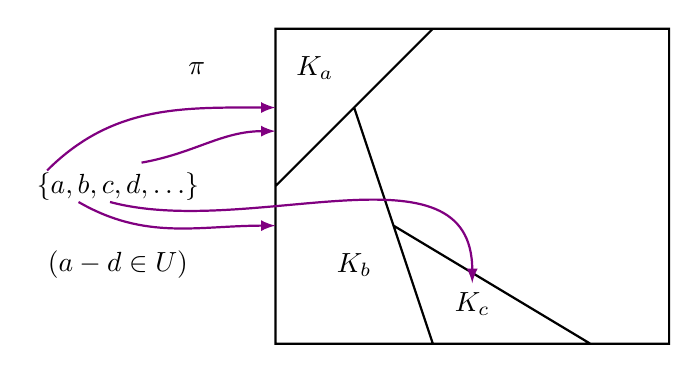
\begin{tikzpicture}
        \draw node at (3, 3.5) {$\pi$}
            node (set) at (2, 2) {$\{a,b,c,d,\ldots\}$}
            node [below of=set] {\normalsize$(a - d \in U)$}
            node (Ka) at (4.5, 3.5) {$K_a$}
            node (Kb) at (5, 1) {$K_b$}
            node (Kc) at (6.5, 0.5) {$K_c$}
            coordinate (a) at (1.1, 2.2)
            coordinate (b) at (1.5, 1.8)
            coordinate (c) at (1.9, 1.8)
            coordinate (d) at (2.3, 2.3);

        % \foreach \x in {1, 1.5, ..., 9}
        %     \foreach \y in {0, 0.5, ..., 4}
        %         \fill[black] (\x, \y) circle (1pt);

        % \foreach \pt in {a, b, c, d}
        %     \fill[red] (\pt) circle (1pt);

        \draw[thick] (4, 0) rectangle (9, 4)
            (4, 2) -- (6, 4)
            (5, 3) -- (6, 0)
            (5.5, 1.5) -- (8, 0);

        \draw[thick,violet,-latex] (a) to[out=45, in=180] (4, 3);
        \draw[thick,violet,-latex] (b) to[out=-30, in=180] (4, 1.5);
        \draw[thick,violet,-latex] (c) to[out=-15, in=90] (Kc);
        \draw[thick,violet,-latex] (d) to[out=10, in=180] (4, 2.7);
    \end{tikzpicture}

    \normalsize
    等价类:仿射子集(如何进一步描述其结构)

    商集:仿射子集构成的集合;商空间:商集上定义加法和数乘

    商映射:自然映射

    商空间的基与维数:两种方法
\end{figure}

\section{线性空间的积}

接下来的两节我们将综合应用之前所学习的基本知识,介绍两个重要的线性空间,即积空间和商空间,以及其上定义的线性映射. 在这两节中我们将完整地展示从定义的引入开始,如何研究一个线性空间,如何合理定义线性映射,如何应用前述知识综合地给出一些空间和映射的性质,这对于我们是一个重要的思维训练.

\subsection{线性空间的积的定义与性质研究}

我们首先探讨线性空间的积,或者积空间. 熟知集合有笛卡尔积运算,而线性空间是定义在集合上的代数结构,因此我们有一个自然的问题,即我们能否在多个线性空间的对应的集合的笛卡尔积上定义加法和数乘运算,使其成为一个线性空间?

答案是肯定的,但我们需要首先声明的一点是,构成笛卡尔积的这些线性空间必须定义在同一个数域上,否则新集合上的数乘我们将很难定义,因为数域不同我们将很难选择数乘的常数应该选择来自于哪个线性空间的数域.
\begin{definition}\label{def:8:积空间}
    设$V_1,V_2,\ldots,V_n$是数域$\mathbf{F}$上的线性空间,我们有如下三个定义:
    \begin{enumerate}
        \item 线性空间的积:
              \[V_1 \times V_2 \times \cdots \times V_n=\{(v_1,v_2,\ldots,v_n)\mid v_i \in V_i,\enspace i=1,2,\ldots,n\};\]

        \item 规定$V_1 \times V_2 \times \cdots \times V_n$上加法和数乘运算:
              \begin{enumerate}
                  \item 加法:$(v_1,v_2,\ldots,v_n)+(u_1,u_2,\ldots,u_n)=(v_1+u_1,v_2+u_2,\ldots,v_n+u_n)$;

                  \item 数乘:$\lambda(v_1,v_2,\ldots,v_n)=(\lambda v_1,\lambda v_2,\ldots,\lambda v_n)$.
              \end{enumerate}
    \end{enumerate}
\end{definition}

事实上我们很容易验证上述定义的线性空间的积在定义的加法和数乘运算下构成线性空间,我们将放在习题中供读者练习. 接下来我们要研究这一线性空间的性质. 事实上,我们早在有限维线性空间一节中就说明了,一个线性空间的核心结构就是其基和维数,因此我们首先研究它们. 事实上,对于积空间,它的基和维数的确定是非常符合我们的直觉的,我们来看一个例子:
\begin{example}
    求积空间$\mathbf{R}[x]_3\times\mathbf{R}^2$的一组基.
\end{example}

\begin{solution}
    我们知道$\mathbf{R}[x]_3$的一组基为$1,x,x^2$,而$\mathbf{R}^2$的一组基为$(1,0),(0,1)$. 很自然的想法是:我们可以先取$\mathbf{R}[x]_3$的一组基,$\mathbf{R}^2$的位置置零,然后反之取$\mathbf{R}^2$的一组基,$\mathbf{R}[x]_3$的位置置零,即$(1,(0,0)),\ (x,(0,0)),\ (x^2,(0,0)),\ (0,(1,0)),\ (0,(0,1))$. 我们很容易可以证明上述向量组满足基的两个条件:线性无关和张成空间.
\end{solution}

上述例子中的基的构造方法是很自然的,而且我们会发现,在这样取基的情况下积空间的维数很显然就是各个线性空间的维数之和. 我们可以很容易地推广到一般情况:
\begin{theorem}\label{thm:8:积空间维数}
    设$V_1,V_2,\ldots,V_n$是数域$\mathbf{F}$上的有限维线性空间,则$V_1 \times V_2 \times \cdots \times V_n$是有限维线性空间,且
    \[\dim(V_1 \times V_2 \times \cdots \times V_n)=\dim V_1+\dim V_2+\cdots+\dim V_n.\]
\end{theorem}

\begin{proof}
    我们取$V_i$的一组基,对这组基中每个向量,我们取$V_1 \times V_2 \times \cdots \times V_n$中的这样的向量:其中第$j$个位置为此向量,其余位置为零向量,这样我们遍历所有$V_i$和每个$V_i$的基向量我们就得到了$V_1 \times V_2 \times \cdots \times V_n$的一组基(线性无关和张成性是很容易验证的),这组基的长度(即维数)为$\dim V_1+\dim V_2+\cdots+\dim V_n$.
\end{proof}

\subsection{线性空间的积与直和}

本节我们将通过线性空间的积的角度来讨论直和的维数特点. 事实上,我们的手段就是构造线性映射,然后利用线性映射基本定理来得到结论.
\begin{theorem}\label{thm:8:积与直和}
    设$U_1,U_2,\ldots,U_n$是$V$的子空间,我们定义线性映射$\sigma:U_1 \times U_2 \times \cdots \times U_n \to U_1+U_2+\cdots+U_n$,使得$\sigma(u_1,u_2,\ldots,u_n)=u_1+u_2+\cdots+u_n$,则$U_1+U_2+\cdots+U_n$是$V$的直和$\iff \sigma$是双射.
\end{theorem}

\begin{proof}
    \begin{enumerate}
        \item 充分性:设$\sigma$是双射,则$\sigma$首先是单射. 根据单射的等价条件,我们有$\ker \sigma=\{0\}$,即$u_1+u_2+\cdots+u_n=0$必须有$u_1=u_2=\cdots=u_n=0$,而这正是\autoref{thm:4:直和等价命题} 中直和的等价条件;

        \item 必要性:设$U_1+U_2+\cdots+U_n$是直和,我们证明$\sigma$是单的、满的:
              \begin{enumerate}
                  \item 单射:设$\sigma(u_1,u_2,\ldots,u_n)=0$,即$u_1+u_2+\cdots+u_n=0$,由直和的等价条件可知$u_1=u_2=\cdots=u_n=0$,即$\sigma$的核空间只有出发空间零元,故是单射;

                  \item 满射:实际上是由这个线性映射的定义直接保证的. $\forall u \in U_1+U_2+\cdots+U_n$,根据和的定义一定有分解$u=u_1+u_2+\cdots+u_n$,其中$u_i \in U_i$,因此根据$\sigma$的定义$\sigma(u_1,u_2,\ldots,u_n)=u$,即任意$u$我们都可找到原像,故是满射.
              \end{enumerate}
    \end{enumerate}
\end{proof}

事实上在证明中我们看到,$\sigma$的定义保证了其满射性,因此定理中最后的双射改为单射也是统一的. 通过这一定理我们可以直接得出以下结论:
\begin{theorem}
    设$U_1,U_2,\ldots,U_n$是有限维线性空间$V$的子空间,则$U_1+U_2+\cdots+U_n$是$V$的直和$\iff \dim(U_1+U_2+\cdots+U_n)=\dim U_1+\dim U_2+\cdots+\dim U_n$.
\end{theorem}

\begin{proof}
    根据\autoref{thm:8:积与直和},$U_1+U_2+\cdots+U_n$是$V$的直和$\iff \sigma$是双射. 我们很容易验证$\sigma$是线性映射,而线性双射我们又称同构映射,同构映射的出发空间和到达空间维数相等,因此$\sigma$是双射$\iff \dim(U_1 \times U_2 \times \cdots \times U_n)=\dim(U_1+U_2+\cdots+U_n)$,最后根据\autoref{thm:8:积空间维数} 积空间的维数可知定理成立.
\end{proof}

这里我们用同构映射完成证明,如果对同构不熟悉的可以回顾定义和等价条件,或者自己用线性映射基本定理进行推导. 由此,我们通过在积空间上定义映射,结合\hyperref[thm:6:线性映射基本定理]{线性映射基本定理}(或同构)得到了\autoref{thm:4:直和等价命题} 中关于维数的命题. 总结而言,在积空间的讨论中我们展现了一个比较完整地学习路径:从定义积空间的想法(来源于集合的笛卡尔积),到如何自然地定义出这一空间的加法和数乘运算,然后研究构造出的空间的基本结构有什么特点,然后进一步构造其上线性映射,得到一些其他的结论. 这一路径的每一步都是非常自然的,而且是学习一个数学概念的常见思路,希望读者不仅是在线性代数中体会到这种学习路径,在其他数学课甚至其他学科中都能总结出这样一条引入—定义—性质—应用的自然路径.

最后我们再看一个拓展的问题,我们希望进一步看到构造同构映射带来的研究问题的方便性:
\begin{example}
    设$V_1,V_2,\ldots,V_n,W$是数域$\mathbf{F}$上的线性空间,证明:$\mathcal{L}(V_1 \times V_2 \times \cdots \times V_n,W)$与$\mathcal{L}(V_1,W) \times \mathcal{L}(V_2,W) \times \cdots \times \mathcal{L}(V_n,W)$同构.
\end{example}
有的读者可能看见这题就会觉得非常简单,因为有限维线性空间的前提下二者维数显然相同,然而我们这里并未限定有限维线性空间,因此需要读者自己构造同构映射.

\begin{solution}
    $\forall f\in \mathcal{L}(V_1 \times V_2 \times \cdots \times V_n,W)$,我们定义$f_i:V_i\to W(i=1,2,\ldots,m)$满足
    \[f_i(v_i)=f(0,\ldots,0,v_i,0,\ldots,0),\]
    其中$v_i$位于第$i$个位置,其余位置为零向量.

    定义$\varphi:\mathcal{L}(V_1 \times V_2 \times \cdots \times V_n,W)\to \mathcal{L}(V_1,W) \times \mathcal{L}(V_2,W) \times \cdots \times \mathcal{L}(V_n,W)$,使得$\varphi(f)=(f_1,f_2,\ldots,f_m)$,则接下来我们要验证$\varphi$就是我们要求的同构映射.
\end{solution}

\section{对偶空间与对偶映射}

本节我们将开始讨论矩阵的另一种很基本的运算:转置. 我们延续之前讨论的风格,首先介绍运算与线性映射之间的关联,然后再讨论其运算性质. 当然,转置与线性映射的关联不再像之前的那样简单明了,而是要首先引入线性空间和线性映射对偶的概念. 注意,这部分内容只在《线性代数应该这样学》中要求,只学习《大学数学:代数与几何》的读者可以选择性略过有关对偶的知识.

\subsection{对偶空间}

说起对偶,我们并不陌生,这一词语一路陪伴了我们从小学到高中的语文课,有``整齐匀称''之美. 在经济学中,我们可以将企业给定生产成本最大化产出的问题,和给定产出最小化成本的问题视为对偶. 我们自然的想法是,要定义线性空间的对偶,那么应当也是与原先的线性空间有着某种一一对应的关系. 接下来我们将开始定义线性空间的和对偶映射,然后逐步挖掘其中匀称之美.

我们首先回顾一下在\autoref{def:3:线性映射的定义} 中定义的线性泛函的概念:
\begin{definition}[线性泛函] \index{xianxingfanhan@线性泛函 (linear functional)}
    线性空间$V(\mathbf{F})$上的\term{线性泛函}是从$V$到$\mathbf{F}$的线性映射,即线性泛函是$\mathcal{L}(V,\mathbf{F})$中的元素.
\end{definition}
有时我们也将线性泛函称为线性函数,实际上它们都表示将$V$中向量映射到数域上的线性映射. 我们来看几个线性泛函的例子:
\begin{enumerate}
    \item 定义$\sigma:\mathbf{F}^n\to\mathbf{F}$为$\sigma(x_1,\ldots,x_n)=c_1x_1+\cdots+c_nx_n$,其中$c_1,\ldots,c_n\in\mathbf{F}$,则$\sigma$是线性泛函;

    \item 定义$\sigma:\mathbf{R}[x]_n\to\mathbf{R}$为$\sigma(p(x))=\displaystyle\int_0^1p(x)\mathrm{d}x$,则$\sigma$是线性泛函.
\end{enumerate}

我们知道,全体$V$到$\mathbf{F}$的线性映射构成的集合$\mathcal{L}(V,\mathbf{F})$也是一个线性空间(因为这只是$\mathcal{L}(V_1,V_2)$的特例),我们将其定义为线性空间$V$的对偶空间:
\begin{definition}[对偶空间] \index{duioukongjian@对偶空间 (dual space)}
    设$V$是数域$\mathbf{F}$上的线性空间,称$\mathcal{L}(V,\mathbf{F})$为$V$的\term{对偶空间},记作$V^*$.
\end{definition}

即线性空间$V$的对偶空间是其上所有线性泛函构成的线性空间. 事实上,我们知道对于有限维线性空间$V_1$和$V_2$而言,若$\dim V_1=n$,$\dim V_2=m$,则$\mathcal{L}(V_1,V_2)$的维数为$mn$. 因此对偶空间$V^*$的维数就是$\dim V$,因为数域构成的线性空间$\mathbf{F}(\mathbf{F})$维数显然为1,因为乘法单位元1就可以作为一组基(1自身线性无关,然后1数乘$\mathbf{F}$中的元素可以得到所有元素,当然同理只要是非零元就可以作为基).

有同学可能会想到$\mathbf{C}(\mathbf{R})$的维数为2,然而如果翻回线性映射的定义就会发现,我们要求两个线性空间的数域是一致的,所以$V(\mathbf{F})$上的线性泛函一定是到$\mathbf{F}(\mathbf{F})$上的.

沿着我们之前研究积空间和商空间的思路,接下来我们的目标非常明确:找到对偶空间的一组基. 我们可以考虑这样一个问题,假定$V$的维数为$n$,其一组基为$\alpha_1,\ldots,\alpha_n$. 由\autoref{thm:5:线性映射唯一确定} 可知,$V$上任一线性泛函$f$都可以由其在$\alpha_1,\ldots,\alpha_n$下的像$f(\alpha_1),\ldots,f(\alpha_n)$唯一确定. 我们考虑如下映射:
\begin{align*}
    \sigma:V^* & \to\mathbf{F}^n                         \\
    f          & \mapsto(f(\alpha_1),\ldots,f(\alpha_n))
\end{align*}
根据唯一确定性我们很容易证明可知$\sigma$是一个线性双射(即同构映射),事实上这也与$V^*$维数为$n$是相符的. 由于同构映射具有保持向量组线性相关性的特点,我们取$\mathbf{F}^n$的自然基$e_1,\ldots,e_n$,则$\sigma^{-1}(e_1),\ldots,\sigma^{-1}(e_n)$就是$V^*$的一组基,我们称其为\term{对偶基}\index{duiouji@对偶基 (dual basis)},记作$f_1,\ldots,f_n$.

我们进一步探究对偶基的性质,根据上面的定义我们知道$f_i=\sigma^{-1}(e_i)$,即$\sigma(f_i)=e_i$,根据$\sigma$定义即$f_i$在$\sigma$下的像$(f(\alpha_1),\ldots,f(\alpha_n))=e_1=(0,\ldots,0,1,0,\ldots,0)$,即第$i$个分量为1,其余分量为0,即$f_i(\alpha_j)=\delta_{ij}$,其中$\delta_{ij}$为Kronecker记号,展开写即
\[f_i(\alpha_j)=\begin{cases}
        1 & i=j     \\
        0 & i\neq j
    \end{cases}\]
这样我们便得到了对偶基. 我们上面的构造利用的是同构映射,因此无需证明线性无关和张成. 实际上直接证明也并不困难,我们将放在习题中供读者练习.

事实上,通过对偶基的表示我们很容易看出对偶基和原空间基的一一对应关系,即对偶基的某个向量(实际上是映射)只有在原空间对应位置的向量下的像才为1,其余向量下的像都为0. 讲到这里,可能很多读者已经觉得十分抽象了,我们可以理一下思路,对偶空间的定义就是全体线性泛函$V^*=\mathcal{L}(V,\mathbf{F})$,因此它的维数显然和$V$相等,并且我们通过了一个同构映射得到了对偶空间的基的表示. 因为对偶空间中的元素是线性映射,因此基向量也只不过是满足一定条件的线性映射罢了,只是这里的表达可能略微复杂不够直观,但我们可以通过例子来熟悉:
\begin{example}
    设$V=\mathbf{R}[x]_3$,对于$g(x)\in V$,定义:
    \[f_1(g(x))=\displaystyle\int_0^1g(x)\,\mathrm{d}x,\enspace f_2(g(x))=\int_0^2g(x)\,\mathrm{d}x,\enspace f_3(g(x))=\int_0^{-1}g(x)\,\mathrm{d}x,\]
    \begin{enumerate}
        \item 证明:$f_1,f_2,f_3$是$V^*$的一组基;

        \item 求出$V$的一组基$g_1(x),g_2(x),g_3(x)$,使得$f_1,f_2,f_3$是$g_1,g_2,g_3$的对偶基.
    \end{enumerate}
\end{example}

\begin{solution}

\end{solution}

\subsection{对偶映射}

接下来我们将介绍一个看起来可能更为抽象的概念——对偶映射. 如果我们有一个线性映射$\sigma:V\to W$,对偶映射的自然想法就是出发空间和到达空间变为对偶空间,于是我们有如下定义:
\begin{definition}[对偶映射] \index{duiouyingshe@对偶映射 (dual map)}
    设$\sigma:V\to W$是线性映射,定义$\sigma^*:W^*\to V^*$为$\sigma^*(f)=f\circ\sigma,\forall f\in W^*$,则称$\sigma^*$为$\sigma$的\term{对偶映射}.
\end{definition}
定义可能略显抽象,我们做一下说明:
\begin{enumerate}
    \item 看定义$\sigma^*(f)=f\circ\sigma,\enspace\forall f\in W^*$,实际上对偶映射只是把自变量$f$复合了一下原映射$\sigma$. 定义式很好记忆,接下来的各个证明都要熟练使用这一定义;

    \item 因为$\sigma^*(f)=f\circ\sigma,\enspace\forall f\in W^*$,其中$\sigma:V\to W,\enspace f:W\to\mathbf{F}$,由映射复合的定义可知$\sigma^*(f):V\to\mathbf{F}$,因此$\sigma^*$的出发空间是$W^*$(参数$f$所在空间),到达空间是$V^*$(像$\sigma^*(f)$所在空间),故$\sigma^*:W^*\to V^*$;

    \item $\sigma^*$满足线性性,因此是线性映射,证明只需使用线性映射复合运算的性质:
          \begin{gather*}
              \sigma^*(f_1+f_2)=(f_1+f_2)\circ\sigma=f_1\circ\sigma+f_2\circ\sigma=\sigma^*(f_1)+\sigma^*(f_2) \\
              \sigma^*(\lambda f)=(\lambda f)\circ\sigma=\lambda(f\circ\sigma)=\lambda\sigma^*(f)
          \end{gather*}

    \item 对偶映射还有以下运算性质:
          \begin{enumerate}
              \item $\forall\sigma,\tau\in\mathcal{L}(V,W),\enspace (\sigma+\tau)^*=\sigma^*+\tau^*$;

              \item $\forall\sigma\in\mathcal{L}(V,W),\enspace \forall\lambda\in\mathbf{F},\enspace (\lambda\sigma)^*=\lambda\sigma^*$;

              \item $\forall\sigma\in\mathcal{L}(V,W),\enspace \forall\tau\in\mathcal{L}(W,U),\enspace (\tau\sigma)^*=\sigma^*\tau^*$.
          \end{enumerate}
          注意这里的前两点也是线性性质,但前面是指线性映射,是映射对于自变量的线性性,这里可以将$^*$看成一种运算,这种运算作用于对偶映射,具有线性性. 我们简要证明一下这三条性质:

          \begin{proof}
              \begin{enumerate}
                  \item $(\sigma+\tau)^*(f)=(f\circ(\sigma+\tau))=(f\circ\sigma)+(f\circ\tau)=\sigma^*(f)+\tau^*(f)=(\sigma^*+\tau^*)(f)$;

                  \item $(\lambda\sigma)^*(f)=(f\circ(\lambda\sigma))=(\lambda(f\circ\sigma))=\lambda(f\circ\sigma)=\lambda\sigma^*(f)=(\lambda\sigma^*)(f)$;

                  \item $(\tau\sigma)^*(f)=(f\circ(\tau\sigma))=((f\circ\tau)\circ\sigma)=\sigma^*(f\circ\tau)=\sigma^*(\tau^*(f))=(\sigma^*\tau^*)(f)$.
              \end{enumerate}
          \end{proof}
          这里的$f$是任意的,因此这三条性质成立. 其中每一条最后一个等号我们回顾线性映射加法、数乘和复合的定义就会发现这一等号就是定义.
\end{enumerate}
这里希望读者能理解我们分点逐步加深理解的整理方式的良苦用心,事实上就是从简单的概念是什么开始,然后清晰地梳理出各种性质. 将来读者在其他课程中学习到了抽象的新概念,也可以试图做这样的整理,更符合一般的学习逻辑.

按照惯例,接下来我们要尝试使用线性映射基本定理研究对偶映射像空间和核空间的性质,然后得到一些推论. 我们从下面几个方面逐步深入讨论:
\begin{enumerate}
    \item 零化子:为了下面进一步的研究,我们首先要给出零化子的概念:
          \begin{definition}[零化子] \index{linghuazi@零化子 (annihilator)}
              对于线性空间$V$的子空间$U$,定义$U$的\term{零化子}$U^0$为
              \[U^0=\{\varphi\in V^*\mid\varphi(u)=0,\forall u\in U\}.\]
          \end{definition}

          对于零化子,我们有以下说明:
          \begin{enumerate}
              \item 根据定义,$U$的零化子实际上就是把$U$中向量全部映射为0的线性泛函;

              \item 我们很容易证明:$U^0$是$V^*$的子空间:
                    \begin{enumerate}
                        \item 非空:$0\in U^0$,零映射一定在$U^0$中;

                        \item 运算封闭:$\forall\varphi_1,\varphi_2\in U^0,\enspace \forall\lambda\in\mathbf{F}$,有
                              \begin{gather*}
                                  (\varphi_1+\varphi_2)(u)=\varphi_1(u)+\varphi_2(u)=0,\enspace\forall u\in U \\
                                  (\lambda\varphi_1)(u)=\lambda\varphi_1(u)=0,\enspace\forall u\in U
                              \end{gather*}
                              因此$\varphi_1+\varphi_2\in U^0,\enspace \lambda\varphi_1\in U^0$;
                    \end{enumerate}

              \item 既然零化子是子空间,那么我们对其基和维数就会十分感兴趣. 事实上,根据零化子$U^0$的定义是将子空间$U$完全映射为0,根据\autoref{thm:5:线性映射唯一确定},这等价于$U^0$中的元素将子空间$U$的基全部映为0. 设$U$的一组基为$\alpha_1,\ldots,\alpha_s$,则$U^0$中的元素$\varphi$满足
                    \begin{equation}\label{eq:9:零化子基}
                        \varphi(\alpha_1)=\cdots=\varphi(\alpha_s)=0.
                    \end{equation}
                    将这组基扩充成$V$的基$\alpha_1,\ldots,\alpha_s,\alpha_{s+1},\ldots,\alpha_n$,则$V^*$的对偶基为$f_1,\ldots,f_n$,其中$f_i(\alpha_j)=\delta_{ij}$,因此满足\autoref{eq:9:零化子基} 的$V^*$的基向量只有$f_{s+1},\ldots,f_n$. 我们自然猜想这就是$U^0$的一组基. 我们来验证:
                    \begin{enumerate}
                        \item 线性无关:证明是平凡的,因为$f_1,\ldots,f_n$是$V^*$的一组基,基向量组线性无关,因此其子向量组线性无关(可以回顾线性相关性的几种理解);

                        \item 张成空间:设$\varphi\in U^0$,由于首先有$\varphi\in V^*$,则它可以被$f_1,\ldots,f_n$线性表示,即
                              \begin{equation}\label{eq:9:零化子线性表示}
                                  \varphi=\lambda_1f_1+\cdots+\lambda_nf_n,\enspace \lambda_1,\ldots,\lambda_n\in\mathbf{F}.
                              \end{equation}
                              根据\autoref{thm:5:线性映射唯一确定} 可知,$\varphi$被其在$\alpha_1,\ldots,\alpha_n$下的像唯一确定. 由于$\varphi\in U^0$,因此$\varphi(\alpha_1)=\cdots=\varphi(\alpha_s)=0$,代入\autoref{eq:9:零化子线性表示} 可得$\lambda_1=\cdots=\lambda_s=0$.

                              进一步我们将$\alpha_{i},\enspace i=s+1,\ldots,n$代入\autoref{eq:9:零化子线性表示} 可得$\lambda_{i}=\varphi(\alpha_i)$,因此$\varphi$可以被$f_{s+1},\ldots,f_n$线性表示为
                              \[\varphi=\varphi(\alpha_{s+1})f_{s+1}+\cdots+\varphi(\alpha_n)f_n.\]
                    \end{enumerate}
                    因此我们可以根据证明过程得到$U^0$的一组基为$f_{s+1},\ldots,f_n$,维数为$n-s$,更一般地我们有
                    \[\dim U^0=\dim V-\dim U.\]
          \end{enumerate}

    \item 对偶映射核空间与像空间的性质:我们不加证明地给出四个结论,它们对应《线性代数应该这样学》的3.107和3.109. 笔者认为教材给出的证明非常清楚,因此不再赘述.
          \begin{theorem}\label{thm:9:对偶映射像和核的性质}
              设$V$和$W$都是有限维线性空间,$\sigma\in\mathcal{L}(V,W)$,则
              \begin{enumerate}
                  \item $\ker\sigma^*=(\im\sigma)^0$;

                  \item $\dim\ker\sigma^*=\dim\ker\sigma+\dim W-\dim V$;

                  \item $\dim\im\sigma^*=\dim\im\sigma$;

                  \item $\im\sigma^*=(\ker\sigma)^0$.
              \end{enumerate}
          \end{theorem}

          事实上很多情况下我们也并不需要背诵这些性质,一方面这只是几个由前面更为基本的概念和定理导出的性质,不具一般性,并且是为了下面更重要的结论铺垫;另一方面即使一定要记忆,它们很强的对称性使得记忆难度不大.

          这一定理有一个非常关键的推论,其重要性大于上述定理,证明非常简单,见《线性代数应该这样学》3.108和3.110:
          \begin{corollary}\label{cor:9:对偶映射单满射}
              设$V$和$W$都是有限维线性空间,$\sigma\in\mathcal{L}(V,W)$,则
              \begin{enumerate}
                  \item $\sigma$是单射当且仅当$\sigma^*$是满射;

                  \item $\sigma$是满射当且仅当$\sigma^*$是单射.
              \end{enumerate}
          \end{corollary}
\end{enumerate}

\subsection{双重对偶空间}

实际上,对偶空间有一个弊端,我们发现$V^*$的对偶基的选取是与$V$的基的选取有关的,因为我们需要首先确定$V$的一组基$\alpha_1,\ldots,\alpha_n$,然后才能得到$V^*$的对偶基$f_1,\ldots,f_n$,满足$f_i(\alpha_j)=\delta_{ij}$,其中$\delta_{ij}$为Kronecker记号.

事实上这并不美观,因为如果我们尝试定义$V$和$V^*$之间的同构,由于这两个空间两组基的强相关性,我们一般需要有如下定义:
\begin{align*}
    \sigma:V                       & \to V^*                   \\
    \alpha=\sum_{i=1}^nx_i\alpha_i & \mapsto\sum_{i=1}^nx_if_i
\end{align*}
我们会发现,这一映射的定义中$\alpha_i$和$f_i$都离不开选取$V$的一组基$\alpha_1,\ldots,\alpha_n$,更通俗地说,在我们取定了$V$的一组基前,我们甚至写不出$V$和$V^*$之间的同构!

为了更容易地理解这一点,我们可以回想以往的线性映射的定义,例如最简单的
\[\sigma(x_1,x_2,x_3)=(x_1-x_2,x_1+x_3,x_2-x_3),\]
我们要求一个任意元素的像,例如$\sigma(1,2,3)$,我并不需要取$\mathbf{R}^3$的自然基还是其他的基也能知道像为$(-1,4,-1)$,然而$V$和$V^*$之间的同构$\sigma$作用于任意向量$\alpha$后的像$\sigma(\alpha)$在未确定$V$的基前是未定义的!我们一定需要$V$的基才能有坐标$x_i$,然后再利用这个坐标结合像空间的基(这组基和$V$的基是有关的)才能得到像,因此这里的同构映射是非常不美观的.

有的读者可能会质疑,即$V$和$V^*$之间的同构真的一定需要建立在取定$V$的基的基础上吗?事实上的确是需要的,更规范的表述需要进一步学习范畴学等更为深入的数学知识,这里我们只给出直觉:因为同构映射实际上建立的是两个空间基的一一对应关系,然而$V^*$的基本身就依赖于$V$的基的选取,因此我们很难在定义同构映射时避免需要先确定$V$的基这一前提.

因此我们会尝试研究$V$的对偶空间$V^*$的对偶空间$V^{**}$,我们称之为\term{双重对偶空间}\index{duioukongjian!shuangchong@双重 (double dual space)}. 由于$V^*=\mathcal{L}(V,\mathbf{F})$,因此$V^{**}=\mathcal{L}(V^*,\mathbf{F})=\mathcal{L}(\mathcal{L}(V,\mathbf{F}),\mathbf{F})$,因此$V^**$中的元素是这样的线性映射:它的自变量是$V$上的线性泛函,它将这一线性泛函映到一个数.

我们知道$\dim V=\dim V^*$,故$V^*$也和其对偶空间有相同的维数,即$\dim V^*=\dim V^{**}$,故$\dim V=\dim V^{**}$,因此我们可以尝试构造一个同构映射$\sigma:V\to V^{**}$,使得这一映射不依赖于$V$的基的选取. 我们发现这样的映射是存在的,我们来跟着下面这个例子逐步说明:
\begin{example}
    设$V$为有限维线性空间. 我们定义$\tau:V\to V^{**}$为
    \[(\tau(\alpha))(f)=f(\alpha),\enspace\forall \alpha\in V,\enspace f\in V^*.\]
    \begin{enumerate}
        \item 证明:$\tau$是线性映射;

        \item 证明:若$\sigma\in\mathcal{L}(V,V)$,则$\sigma^{**}\circ\tau=\tau\circ\sigma$,这里$\sigma^{**}$是$\sigma^*$的对偶映射;

        \item 证明:$\tau$是$V$到$V^{**}$的同构映射.
    \end{enumerate}
\end{example}

\begin{solution}

\end{solution}

我们发现这一同构映射不需要先确定$V$的基就可以定义,因此相对于$V$与$V^*$间的同构映射更为自然. 在范畴学中,我们称这样的映射为
\term{自然同构}\index{tonggou!ziran@自然同构 (natural isomorphism)},它不依赖于选取的基,一直客观存在着,就好像在等着我们发现一样,而$V$与$V^*$间的同构映射则需要通过我们先取出$V$的基才能定义,因此缺少了这样``自然''的客观存在的感觉.

事实上本节的讨论是比较抽象的,我们只能通过一些例子和描述来直观理解其中核心的思想,即自然同构中``自然''的含义(不依赖于基的选取). 我们长篇的论述的核心就是直观地告诉读者,$V$和$V^*$之间找不到自然同构,但$V$和$V^{**}$之间存在. 更深入、严谨的讨论可能需要读者进一步学习范畴学的相关知识才能全面理解.

\section{对偶映射的矩阵}

有了前述内容的铺垫,本节我们将最终给出对偶映射的矩阵. 我们首先介绍矩阵转置的概念,然后说明对偶为什么与转置相关.
\begin{definition}[转置] \index{zhuanzhi@转置 (transpose)}
    设$A=\begin{pmatrix}
            a_{11} & a_{12} & \cdots & a_{1n} \\
            a_{21} & a_{22} & \cdots & a_{2n} \\
            \vdots & \vdots & \ddots & \vdots \\
            a_{m1} & a_{m2} & \cdots & a_{mn}
        \end{pmatrix}$,称$\begin{pmatrix}
            a_{11} & a_{21} & \cdots & a_{m1} \\
            a_{12} & a_{22} & \cdots & a_{m2} \\
            \vdots & \vdots & \ddots & \vdots \\
            a_{1n} & a_{2n} & \cdots & a_{mn}
        \end{pmatrix}$为矩阵$A$的\term{转置},记作$A^\mathrm{T}$.
\end{definition}

简单来说,矩阵的转置就是矩阵的第$i$行变成了第$i$列(或者第$i$列变成了第$i$行,即行列互换),原先矩阵第$i$行第$j$列的元素转置后变为第$j$行第$i$列的元素,或者抽象表达为:
\[A=(a_{ij})_{m \times n},\enspace A^\mathrm{T}=(a'_{ji})_{n \times m},\enspace a_{ij}=a'_{ji}\]

接下来我们将说明对偶映射在对偶基下的矩阵就是原映射在原空间基下矩阵的转置:
\begin{theorem}
    $V$和$W$为有限维线性空间. $V$的一组基为$\alpha_1,\ldots,\alpha_n$,$W$的一组基为$\beta_1,\ldots,\beta_m$,它们对偶空间的基分别为$f_1,\ldots,f_n$和$g_1,\ldots,g_m$. 设$\sigma\in\mathcal{L}(V,W)$,它在上述$V$和$W$的基下的矩阵为$A=(a_{ij})_{m \times n}$,则$\sigma^*\in\mathcal{L}(W^*,V^*)$在上述对偶基下的矩阵为$C=(c_{ij})_{n \times m}=A^\mathrm{T}$.
\end{theorem}

\begin{proof}
    根据线性映射矩阵表示的定义,我们有
    \[\sigma^*(g_j)=\sum_{i=1}^nc_{ij}f_i,\enspace j=1,2,\ldots,m.\]
    上式左端根据对偶映射定义等于$(g_j\circ\sigma)$. 于是我们将等式两端均作用于$\alpha_k$上有
    \[(g_j\circ\sigma)(\alpha_k)=\sum_{i=1}^nc_{ij}f_i(\alpha_k)=\sum_{i=1}^nc_{ij}\delta_{ik}=c_{kj}.\]
    另一方面,根据映射复合的结合律以及线性映射矩阵表示的定义,我们有
    \[(g_j\circ\sigma)(\alpha_k)=g_j(\sigma(\alpha_k))=g_j\left(\sum_{i=1}^na_{ik}\beta_i\right)=\sum_{i=1}^na_{ik}g_j(\beta_i)=\sum_{i=1}^na_{ik}\delta_{ij}=a_{jk}.\]
    因此我们有$c_{kj}=a_{jk}$,即$C=A^\mathrm{T}$.
\end{proof}

可能由许多同学心存疑惑——我们为什么要费这么大劲介绍一个这么特别且抽象的概念然后引入转置?事实上对偶这一概念在数学中是非常重要的,在之后我们还将提起它,现在可以先留下一个美好的期待,相信在之后的学习中你会逐渐发现这一定义是自然而美妙的,而且其中蕴含的思想是有很大的应用价值的.

除此之外,在这一讲中笔者也反复强调,面对这一抽象的内容我们不要畏惧,我们可以先从是什么开始,熟练概念,然后理解相关的性质,例如我们在定义对偶映射的时候就强调先记住很好记忆的定义式,然后我们再说明它的出发空间、到达空间是什么,具有什么样的性质,不能一开始就妄图直接装下所有的概念、性质,这样只能使思维混乱且不知道自己学了什么. 我们应当学会将抽象的概念通过拆解成大家从小就习惯的``是什么''的教育和研究中更感兴趣的内容两部分进行梳理,从而更快地理解.

\vspace{2ex}
\centerline{\heiti \Large 内容总结}

事实上,这一讲是本讲义第一次接触技巧性较强的内容,我们的重点从之前对于定理的证明以及用例子巩固定理的应用转变为了对于一些技巧性的处理. 我们首先介绍了三类初等变换(请务必注意正文中强调的几个定义的细节),证明了任意可逆矩阵都可以被表示成若干初等矩阵的乘积,也基于此引出了第二种求解逆矩阵的方法——初等变换法,这也是我们未来最常用的方法. 除此之外,我们也联系了线性映射矩阵表示和初等变换,研究了高斯消元法背后的合理性.

接下来我们介绍了分块矩阵的基本运算性质,比较了分块矩阵和一般矩阵运算的异同(特别是乘法和转置),介绍了两种分块矩阵求逆的方法:其一直接设出逆矩阵,其二利用所谓打洞法(分块矩阵初等变换),其中打洞法是一个很重要的技巧,虽然教材列为小字部分,考试中一般不考察,但拥有这一技巧对我们未来证明很多结论都有很大的帮助. 最后我们介绍了矩阵方程的求解方法,本质而言介绍了几种基于初等变换的求解方法,读者理解其内涵即可.

\vspace{2ex}
\centerline{\heiti \Large 习题}

\vspace{2ex}
{\kaishu 龙生龙,凤生凤,华罗庚的学生会打洞.}
\begin{flushright}
    \kaishu
    ——线性代数教学俗语
\end{flushright}

\centerline{\heiti A组}
\begin{enumerate}
    \item 设$A$为三阶矩阵,将$A$的第二列加到第一列得到矩阵$B$,再对调$B$的2、3行得到单位矩阵. 令$P_1=\begin{pmatrix}1 & 0 & 0 \\ 1 & 1 & 0 \\ 0 & 0 & 1\end{pmatrix}\enspace
              P_2=\begin{pmatrix}1 & 0 & 0 \\ 0 & 0 & 1 \\ 0 & 1 & 0\end{pmatrix}$,试用$P_1$和$P_2$表示$A$.

    \item 设$A$为可逆矩阵,将$A$的第$i$行和第$j$行对调得到矩阵$B$,证明矩阵$B$可逆并求$AB^{-1}$.

    \item 设$A$为三阶可逆矩阵,且$P^{-1}AP=\begin{pmatrix}1 & 0 & 0 \\ 0 & 1 & 0 \\ 0 & 0 & 2\end{pmatrix}$,其中$P=(\alpha_1,\alpha_2,\alpha_3)$,令$Q=(\alpha_1+\alpha_2,\alpha_2,\alpha_3)$,求$Q^{-1}AQ$.

    \item 求下列矩阵的可逆的条件与逆矩阵:$\begin{pmatrix}
                  A & B \\ O & D
              \end{pmatrix},\enspace \begin{pmatrix}
                  O & B \\ C & D
              \end{pmatrix}$.
\end{enumerate}

\centerline{\heiti B组}
\begin{enumerate}
    \item 已知$\mathbf{R}^3$的基$B_1=\{\alpha_1,\alpha_2,\alpha_3\}$变为基$B_2=\{\xi_1,\xi_2,\xi_3\}$的变换矩阵为$A=(a_{ij})_{3 \times 3}$,求:
          \begin{enumerate}
              \item 基$B_3=\{\alpha_2,\alpha_1,\alpha_3\}$变为基$B_2$的变换矩阵;

              \item 基$B_4=\{-\alpha_1,\alpha_2,\alpha_3\}$变为基$B_2$的变换矩阵;

              \item 基$B_4$变为基$B_5=\{\xi_3,\xi_2,-\xi_1\}$的变换矩阵;

              \item 基$B_4$变为基$B_6=\{\xi_1+\xi_2,\xi_2+\xi_3,\xi_3+\xi_1\}$的变换矩阵.
          \end{enumerate}

    \item 设$P=\begin{pmatrix}
                  1 & 1 & 0 \\ 0 & 1 & 0 \\ 0 & 0 & 0
              \end{pmatrix}$,$Q=\begin{pmatrix}
                  0 & 0 \\ 1 & 0
              \end{pmatrix}$,定义$\mathbf{R}^{3\times 2}$上映射$\sigma(A)=PAQ$.
          \begin{enumerate}
              \item 验证$\sigma$是线性映射;

              \item 求$\ker\sigma$和$\im \sigma$;

              \item 求$\mathbf{R}^{3\times 2}$的两组基,使得$\sigma$关于这两组基的表示矩阵是对角矩阵.
          \end{enumerate}

    \item % 新题,需要答案
\end{enumerate}

\centerline{\heiti C组}
\begin{enumerate}
    \item 若$n$阶矩阵$A$的各阶左上角子块矩阵都可逆,则存在$n$阶下三角矩阵$B$,使得$BA$为上三角矩阵.

    \item 设$A$是数域$\mathbf{F}$上的$n$阶可逆矩阵,把$A$和$A^{-1}$做如下分块:
          \[A=\begin{pmatrix}
                  A_{11} & A_{12} \\ A_{21} & A_{22}
              \end{pmatrix},\enspace A^{-1}=\begin{pmatrix}
                  B_{11} & B_{12} \\ B_{21} & B_{22}
              \end{pmatrix}\]
          其中$A_{11}$是$l \times k$矩阵,$B_{11}$是$k \times l$矩阵,$l$,$k$是小于$n$的正整数. 用$W$表示$A_{12}X=0$的解空间,$U$表示$B_{12}Y=0$的解空间,其中$X$和$Y$为列向量,证明$W$与$U$同构.

    \item $A$的Schur补以及商等式$A/B=(A/C)/(B/C)$% 新题,需要答案
\end{enumerate}
 % 射影空间
\LUchapter{多重线性映射与张量的计算}

\chapter{行列式}

接下来我们将开始介绍大部分线性代数或高等代数教材中开头就会介绍的内容——行列式. 在本讲义的思路中,我们更多将行列式视为一个帮助我们研究的工具,无论是当前的主线——线性方程组解的理论还是之后我们要介绍的矩阵标准形的内容. 因此我们会将这一章只作类似``工具介绍''的作用,而非其他教材那样从行列式出发引出相关概念,因为我们研究的核心和出发点是之前的抽象空间和映射.

事实上,我们将在本讲义之后再介绍一次行列式,那时我们将会介绍行列式更丰富的应用,并表明是否引入行列式可能对于线性代数完整理论的构建而言重要程度是有限的. 但是我们完全无法否认行列式的历史地位,从17世纪起行列式就是用于求解线性方程组的重要的工具,历经数百年也逐渐发展出了许多重要的理论和应用,因此我们仍然需要完整的章节来讲述行列式的相关内容.

\section{行列式的定义}

很多教材采用``逆序数''定义行列式,但是本教材未提及,而且也缺乏直观,因此我们不在本讲展开描述. 我们会在史海拾遗中结合历史给出相关的定义,当然感兴趣的同学可以参考丘维声《高等代数》等教材. 本教材使用公理化定义(使用一些规则描述)并讲解了递归式定义(按行(列)展开).

\subsection{公理化定义}

\begin{definition}{行列式}{公理化定义} \index{hanglieshi@行列式 (determinant)}
    数域$\mathbf{F}$上的一个$n$阶\term{行列式}是取值于$\mathbf{F}$的$n$个$n$维向量$\alpha_1,\alpha_2,\ldots,\alpha_n \in \mathbf{F}^n$的一个函数,且$\forall \alpha_i,\beta_i \in \mathbf{F}^n$和$\forall \lambda \in \mathbf{F}$,满足下列规则:
    \begin{enumerate}
        \item \label{item:13:齐性}
              (齐性) $D(\alpha_1,\ldots,\lambda\alpha_i,\ldots,\alpha_n)=\lambda D(\alpha_1,\ldots,\alpha_i,\ldots,\alpha_n)$;

        \item \label{item:13:加性}
              (加性,与 \ref*{item:13:齐性} 合称线性性) \\
              $D(\alpha_1,\ldots,\alpha_i+\beta_i,\ldots,\alpha_n)=D(\alpha_1,\ldots,\alpha_i,\ldots,\alpha_n)+D(\alpha_1,\ldots,\beta_i,\ldots,\alpha_n)$;

        \item \label{item:13:反对称性}
              (反对称性) $D(\alpha_1,\ldots,\alpha_i,\ldots,\alpha_j,\ldots,\alpha_n)=-D(\alpha_1,\ldots,\alpha_j,\ldots,\alpha_i,\ldots,\alpha_n)$;

        \item \label{item:13:规范性}
              (规范性) $D(e_1,e_2,\ldots,e_n)=1$.
    \end{enumerate}
\end{definition}
在公理化定义中,我们将行列式定义为一个满足特定的运算性质的从列向量组合到数的函数. 事实上,公理化定义从是逆序数定义可以推导出的行列式的运算性质,教材采用这种定义避开了繁琐的说明.

除此之外,我们不难看出公理化定义可以形象地理解为对$n$维空间中体积的定义,对几何意义感兴趣的同学可以参考 \href{https://b23.tv/BV1ys411472E}{3b1b《线性代数的本质》系列视频}相关内容.
\begin{example}{}{公理化定义}
    使用\autoref{def:公理化定义} 验证下述命题的正确性:
    \begin{enumerate}
        \item 若行列式有一列为零向量,则行列式的值等于0.

        \item 若行列式有两列元素相同,则行列式的值等于0.

        \item 若行列式有两列元素成比例,则行列式的值等于0.

        \item 对行列式做倍加列变换,行列式的值不变.

        \item 若$\alpha_1,\alpha_2,\ldots,\alpha_n$线性相关,则$D(\alpha_1,\alpha_2,\ldots,\alpha_n)=0$.
    \end{enumerate}
\end{example}

\begin{proof}
    \begin{enumerate}
        \item 由于行列式满足\autoref{def:公理化定义} 的\ref*{item:13:齐性},设行列式第$i$列为零向量,因此
              \begin{align*}
                  D(\alpha_1,\ldots,0,\ldots,\alpha_n) & =D(\alpha_1,\ldots,0\cdot\alpha_i,\ldots,\alpha_n)  \\
                                                       & =0\cdot D(\alpha_1,\ldots,\alpha_i,\ldots,\alpha_n) \\
                                                       & =0
              \end{align*}

        \item 由于行列式满足\autoref{def:公理化定义} 的\ref*{item:13:反对称性},设行列式第$i$列和第$j$列元素相同,因此
              \begin{align*}
                  D(\alpha_1,\ldots,\alpha_i,\ldots,\alpha_j,\ldots,\alpha_n) & =D(\alpha_1,\ldots,\alpha_j,\ldots,\alpha_i,\ldots,\alpha_n)  \\
                                                                              & =-D(\alpha_1,\ldots,\alpha_i,\ldots,\alpha_j,\ldots,\alpha_n)
              \end{align*}
              从而$D(\alpha_1,\ldots,\alpha_i,\ldots,\alpha_j,\ldots,\alpha_n)=0$.

        \item 由于行列式满足\autoref{def:公理化定义} 的\ref*{item:13:齐性},设行列式第$i$列和第$j$列元素成比例,$\alpha_i=k\alpha_j$,因此
              \begin{align*}
                  D(\alpha_1,\ldots,\alpha_i,\ldots,\alpha_j,\ldots,\alpha_n)
                   & =D(\alpha_1,\ldots,k\alpha_j,\ldots,\alpha_j,\ldots,\alpha_n) \\
                   & =kD(\alpha_1,\ldots,\alpha_j,\ldots,\alpha_j,\ldots,\alpha_n) \\
                   & =0
              \end{align*}
              其中最后一个等号用到了本例的第二条结论.

        \item 事实上,根据\autoref{def:公理化定义} 的\ref*{item:13:加性} 以及本例第3条结论,我们可以得到
              \begin{align*}
                  D(\alpha_1,\ldots,\alpha_i+k\alpha_j,\ldots,\alpha_j,\ldots,\alpha_n)
                   & =D(\alpha_1,\ldots,\alpha_i,\ldots,\alpha_j,\ldots,\alpha_n)   \\&+D(\alpha_1,\ldots,k\alpha_j,\ldots,\alpha_j,\ldots,\alpha_n) \\
                   & =D(\alpha_1,\ldots,\alpha_i,\ldots,\alpha_j,\ldots,\alpha_n)+0 \\
                   & =D(\alpha_1,\ldots,\alpha_i,\ldots,\alpha_j,\ldots,\alpha_n).
              \end{align*}

        \item 设$\alpha_1,\alpha_2,\ldots,\alpha_n$线性相关,因此存在不全为0的数$k_1,k_2,\ldots,k_n$使得$k_1\alpha_1+k_2\alpha_2+\cdots+k_n\alpha_n=0$,不妨设$k_1 \neq 0$,因此
              \[\alpha_1=-\frac{k_2}{k_1}\alpha_2-\frac{k_3}{k_1}\alpha_3-\cdots-\frac{k_n}{k_1}\alpha_n,\]
              因此
              \begin{align*}
                  D(\alpha_1,\alpha_2,\ldots,\alpha_n) & =D(-\frac{k_2}{k_1}\alpha_2-\frac{k_3}{k_1}\alpha_3-\cdots-\frac{k_n}{k_1}\alpha_n,\alpha_2,\ldots,\alpha_n)     \\
                                                       & =-\frac{k_2}{k_1}D(\alpha_2,\alpha_2,\ldots,\alpha_n)-\cdots-\frac{k_n}{k_1}D(\alpha_n,\alpha_2,\ldots,\alpha_n) \\
                                                       & =0.
              \end{align*}
    \end{enumerate}
\end{proof}

\begin{example}{}{公理化定义2}
    设向量$\alpha_1,\alpha_2,\beta_1,\beta_2$为三维列向量,又$A=(\alpha_1,\alpha_2,\beta_1),B=(\alpha_1,\alpha_2,\beta_2)$,且$|A|=3$,$|B|=2$,求$|2A+3B|$.
\end{example}

\begin{solution}
    $2A+3B=(2\alpha_1+3\alpha_1,2\alpha_2+3\alpha_2,2\beta_1+3\beta_2)=(5\alpha_1,5\alpha_2,2\beta_1+3\beta_2)$,因此
    \begin{align*}
        |2A+3B| & =|5\alpha_1,5\alpha_2,2\beta_1+3\beta_2|                       \\
                & =25|\alpha_1,\alpha_2,2\beta_1+3\beta_2|                       \\
                & =25(2|\alpha_1,\alpha_2,\beta_1|+3|\alpha_1,\alpha_2,\beta_2|) \\
                & =25(2|A|+3|B|)=300.                                            \\
    \end{align*}
\end{solution}

\subsection{递归式定义}

首先我们需要引入余子式和代数余子式的概念:
\begin{definition}{}{余子式}
    在$n$阶行列式$D=|a_{ij}|_{n \times n}$中,去掉元素$a_{ij}$所在的第$i$行和第$j$列的所有元素而得到的$n-1$阶行列式称为元素$a_{ij}$的\term{余子式}\index{yuzishi@余子式 (minor)},记作$M_{ij}$,并把数$A_{ij}=(-1)^{i+j}M_{ij}$称为元素$a_{ij}$的\term{代数余子式}\index{yuzishi!daishu@代数余子式 (cofactor)}.
\end{definition}
注意,虽然余子式和代数余子式在名称中含有式,但实际上他们是一个值. 实际上行列式也称为``式'',但这些``式''只是形状上有个形式,实际上只是一个值.
\begin{example}{}{余子式}
    根据\autoref{def:余子式} 计算行列式$\begin{vmatrix}
            2  & 1 & 3  \\
            -1 & 0 & 2  \\
            1  & 5 & -2
        \end{vmatrix}$每个元素的余子式和代数余子式.
\end{example}

\begin{solution}
    我们只举一个例子,第二行第一列元素$-1$的余子式和代数余子式. 根据定义,它的余子式是去掉第二行和第一列所有元素剩余的二阶行列式
    \[\begin{vmatrix}
            1 & 3  \\
            5 & -2
        \end{vmatrix}=-17,\]
    因此它的代数余子式是$A_{21}=(-1)^{2+1}(-17)=17$. 读者可以自行计算其他元素的余子式和代数余子式.
\end{solution}

接下来我们便可以给出递归式定义:
\begin{definition}{}{递归式定义}
    设$D=|a_{ij}|_{n \times n}$,则
    \begin{align}
        \label{eq:13:递归式定义1}
        D=\sum_{k=1}^{n}a_{kj}A_{kj}=a_{1j}A_{1j}+a_{2j}A_{2j}+\cdots+a_{nj}A_{nj} & \qquad j=1,2,\ldots,n \\
        \label{eq:13:递归式定义2}
        D=\sum_{k=1}^{n}a_{ik}A_{ik}=a_{i1}A_{i1}+a_{i2}A_{i2}+\cdots+a_{in}A_{in} & \qquad i=1,2,\ldots,n
    \end{align}
\end{definition}
其中$A_{ij}$即为\autoref{def:余子式} 给出的代数余子式,\autoref{eq:13:递归式定义1} 称为$D$对第$j$列的展开式,\autoref{eq:13:递归式定义2} 称为$D$对第$i$行的展开式. 事实上,这一定义被称为递归式定义的原因是显然的(如果在程序设计课程中已经学习过递归的概念),它使用$n-1$阶行列式定义$n$阶行列式,因此我们对任意$n$阶行列式都可以递归展开到1阶,从而得到最终行列式计算结果.

除此之外,我们需要强调的是,这里的递归式定义能称之为定义,必须要使得其与之前的公理化定义不冲突. 事实上二者等价的证明都是技术性的,教材175页定理5.1说明了我们如何从公理化定义推出递归式定义,反过来我们只需要对公理化定义中每个性质利用公理化定义逐个展开验算即可,我们放在习题中供感兴趣的读者自行验证. 因为都是技术性的问题,这里不展开叙述,事实上也不是我们核心的内容.
\begin{example}{}{递归式定义}
    利用\autoref{def:递归式定义} 计算\autoref{ex:余子式} 中的行列式,可以行列展开均使用并在上述公式中选取不同$i$和$j$以熟悉\autoref*{def:递归式定义},并注意体会递归式定义的含义.
\end{example}

\begin{solution}
    我们选取$i=2$进行按行展开,由\autoref{def:余子式} 可知$A_{21}=17,A_{22}=-7,A_{23}=-9$,因此
    \begin{align*}
        D & =\sum_{k=1}^{3}a_{2k}A_{2k}              \\
          & =a_{21}A_{21}+a_{22}A_{22}+a_{23}A_{23}  \\
          & =(-1) \cdot 17+0 \cdot (-7)+2 \cdot (-9) \\
          & =-35.
    \end{align*}
    同理,我们选取$j=3$进行按列展开,由\autoref{def:余子式} 可知$A_{13}=-5,A_{23}=-9,A_{33}=1$,因此
    \begin{align*}
        D & =\sum_{k=1}^{3}a_{k3}A_{k3}             \\
          & =a_{13}A_{13}+a_{23}A_{23}+a_{33}A_{33} \\
          & =3 \cdot (-5)+2 \cdot (-9)+(-2) \cdot 1 \\
          & =-35.
    \end{align*}
    读者可以自行计算按其他行列展开的结果.
\end{solution}

递归式定义有一个重要的结论如下:
\begin{theorem}{}{递归性质}
    $n$阶行列式$D=|a_{ij}|_{n \times n}$的某一行(列)元素与另一行(列)相应元素的代数余子式的乘积之和等于0,即
    \begin{align}
        \label{eq:13:递归式定义3}
        \sum_{k=1}^{n}a_{kj}A_{ki}=a_{1j}A_{1i}+a_{2j}A_{2i}+\cdots+a_{nj}A_{ni}=0 & \qquad j \neq i \\
        \label{eq:13:递归式定义4}
        \sum_{k=1}^{n}a_{jk}A_{ik}=a_{j1}A_{i1}+a_{j2}A_{i2}+\cdots+a_{jn}A_{in}=0 & \qquad j \neq i
    \end{align}
\end{theorem}

我们简要说一下定理的证明. 虽然这一定理看着下标满天飞,似乎很难证明,但如果我们首先将第$j$列元素替换为第$i$列元素,然后根据\autoref{def:递归式定义} 按第$j$列展开求行列式,这一结果一定是0,因为此时矩阵第$i$和$j$两列完全相同. 同时我们发现,我们上面展开写出的式子就是\autoref{eq:13:递归式定义3}(注意此时$a_{ki}=a_{kj}$),由此得证.

到目前为止,读者可能对\crefrange*{eq:13:递归式定义1}{eq:13:递归式定义4} 式繁杂的下标感到陌生,因此安排了\crefrange*{ex:公理化定义2}{ex:递归式定义} 希望大家熟悉这些公式.
\begin{example}{}{递归式定义2}
    对\autoref{ex:递归式定义} 中的矩阵验证\autoref{thm:递归性质} 的正确性.
\end{example}

\begin{solution}
    例如我们选取第一行元素和第二行的代数余子式,由\autoref{def:余子式} 可知$A_{21}=17,A_{22}=-7,A_{23}=-9$,因此
    \begin{align*}
        D & =\sum_{k=1}^{3}a_{1k}A_{2k}             \\
          & =a_{11}A_{21}+a_{12}A_{22}+a_{13}A_{23} \\
          & =2 \cdot 17+1 \cdot (-7)+3 \cdot (-9)   \\
          & =0.
    \end{align*}
\end{solution}

这一节中行列式是按照一行(列)展开的,若按多行(列)展开则需要相应的 Laplace 定理,我们将在下一讲行列式计算进阶中介绍.

\subsection{行列式的常用性质}

设$A,B \in \mathbf{F}^{n \times n}$,$k \in \mathbf{F}$,则
\begin{enumerate}
    \item 一般情况下,$|A \pm B| \neq |A|\pm|B|$;

    \item $|kA|=k^n|A|$;
          \begin{proof}
              由\autoref{def:公理化定义} 的\ref*{item:13:齐性},设$A=(\alpha_1,\alpha_2,\ldots,\alpha_n)$,则
              \begin{align*}
                  |kA| & =|k\alpha_1,k\alpha_2,\ldots,k\alpha_n| \\
                       & =k^n|\alpha_1,\alpha_2,\ldots,\alpha_n| \\
                       & =k^n|A|.
              \end{align*}
          \end{proof}

    \item \label{item:13:行列式性质:4}
          初等矩阵行列式(注意初等矩阵不分行列,左乘右乘区分初等行列变换):\\
          $|E_{ij}|=-1,\enspace |E_i(c)|=c,\enspace |E_{ij}(k)|=1$;

    \item 利用 \ref*{item:13:行列式性质:4} 中的结论可以得到$|AB|=|A||B|,\enspace|A^k|=|A|^k$;

    \item 利用 \ref*{item:13:行列式性质:4} 中的结论可以得到$A$可逆$\iff |A| \neq 0$;

    \item 利用 \ref*{item:13:行列式性质:4} 中的结论可以得到$|A^\mathrm{T}|=|A|$;

    \item 利用 \ref*{item:13:行列式性质:4} 中的结论可以得到上、下三角矩阵行列式均为主对角线元素的乘积;

    \item 利用 \ref*{item:13:行列式性质:4} 中的结论(求出初等矩阵逆矩阵行列式)可以得到若$A$可逆,则$|A^{-1}|=|A|^{-1}$.
          \begin{proof}
              由$|AB|=|A||B|$,设$B=A^{-1}$,则$|E|=|AA^{-1}|=|A||A^{-1}|$,因此$|A||A^{-1}|=1$,从而$|A^{-1}|=|A|^{-1}$.
          \end{proof}
\end{enumerate}

以上性质都可以基于定义或上述其他性质得到,其中3-6条可参考教材5.3节,7可参考教材172页例3. 这些性质结论希望读者熟悉,实际上推导过程重要性不大,虽然也并不复杂. 下面介绍的性质需要用到``打洞法''(分块矩阵初等变换)来证明:

\begin{enumerate}
    \item $\begin{vmatrix}
                  A & O \\ O & B
              \end{vmatrix} = \begin{vmatrix}
                  A & O \\ C & B
              \end{vmatrix} = \begin{vmatrix}
                  A & D \\ O & B
              \end{vmatrix} = |A||B|,\enspace\begin{vmatrix}
                  O & A \\ B & C
              \end{vmatrix} = (-1)^{kr}|A||B|$(其中$A$为$k$阶方阵,$B$为$r$阶方阵);
          \begin{proof}
              证明从略,感兴趣的读者可以参考教材179页例2,实际上我们很多时候只需要基于这些结论证明进一步的性质.
          \end{proof}

    \item 当$A$可逆时,有$\begin{vmatrix}
                  A & B \\ C & D
              \end{vmatrix} = |A||D-CA^{-1}B|$,当$D$可逆时,有$\begin{vmatrix}
                  A & B \\ C & D
              \end{vmatrix} = |D||A-BD^{-1}C|$,当$B$可逆时,有$\begin{vmatrix}
                  A & B \\ C & D
              \end{vmatrix} = (-1)^{mn}|B||C-DB^{-1}A|$,当$C$可逆时,有$\begin{vmatrix}
                  A & B \\ C & D
              \end{vmatrix} = (-1)^{mn}|C||B-AC^{-1}D|$;
          \begin{proof}
              由于
              \[\begin{pmatrix}
                      E & O \\ -CA^{-1} & E
                  \end{pmatrix}\begin{pmatrix}
                      A & B \\ C & D
                  \end{pmatrix}= \begin{pmatrix}
                      A & B \\ O & D-CA^{-1}B
                  \end{pmatrix},\]
              两边取行列式,并注意到
              \[\begin{vmatrix}
                      E & O \\ -CA^{-1} & E
                  \end{vmatrix}=1,\]
              因此
              \[\begin{vmatrix}
                      A & B \\ C & D
                  \end{vmatrix}=\begin{vmatrix}
                      A & B \\ O & D-CA^{-1}B
                  \end{vmatrix}=|A||D-CA^{-1}B|.\]

              读者会发现,我们在上面的证明中多次使用$\begin{vmatrix}
                      A & O \\ C & B
                  \end{vmatrix} = \begin{vmatrix}
                      A & D \\ O & B
                  \end{vmatrix} = |A||B|$这一性质,因此这一性质是相当重要的,需要读者熟悉.

              本条的其他结论推导类似于上方,在此不再赘述,感兴趣的读者可以自行推导(关键在于第三类分块初等矩阵行列式为1),实际上结论并不是很重要,重要的是在于领悟使用行列式分块计算性质和打洞法的基本方法.
          \end{proof}

    \item 设$A,B$分别是$n \times m$和$m \times n$矩阵,则$|E_n \pm AB|=|E_m \pm BA|$,且 \\
          $|\lambda E_n \pm AB|=\lambda^{n-m}|\lambda E_m \pm BA|,\enspace n \geqslant m$.
          \begin{proof}
              由前述第二条性质直接可得
              \[|E_n \pm AB|=\begin{vmatrix}
                      E_n & A \\ \mp B & E_m
                  \end{vmatrix}=|E_m \pm BA|,\]
              也有
              \begin{align*}
                  |\lambda E_n \pm AB|
                   & =\begin{vmatrix}
                          \lambda E_n & A \\ \mp B & E_m
                      \end{vmatrix}=\lambda^n
                  \begin{vmatrix}
                      E_n & \lambda^{-1}A \\ \mp B & E_m
                  \end{vmatrix}=\lambda^{n-m}\begin{vmatrix}
                                                 E_n & A \\ \mp B & E_m
                                             \end{vmatrix} \\
                   & = \lambda^{n-m}|\lambda E_m \pm BA|.
              \end{align*}
              其中第一行第二个等号来源于前$n$行每行提出一个$\lambda$,第一行第三个等号来源于后$m$列每列乘以$\lambda$.
          \end{proof}

          事实上,这里的结果在特征值与特征向量的部分中我们会给出更深入的解释.
\end{enumerate}

还有一部分由这些性质可以推导的其他性质将出现在C组习题中供参考. 这部分主要是技巧性内容,可以选择性完成.

\section{行列式的基本运算}

本节内容按照往年经验不是考试重点,但是我们要保证教材中涉及的的方法都掌握. 本节我们简要说明教材中提及的基本行列式计算方法,在下一讲行列式计算进阶中我们将用一整讲详细展开行列式的计算技巧.

首先我们用一个简单的三阶行列式的例子回顾行列式的多种基本计算方法. 这里选取三阶行列式主要原因也是三阶行列式在未来实际解题中最为常见,这里希望读者比较选择最适合自己的方法在未来更便捷地使用:
\begin{example}{}{}
    计算行列式$D=\begin{vmatrix}
            1 & 2 & 3 \\
            2 & 3 & 1 \\
            3 & 1 & 2
        \end{vmatrix}$.
\end{example}

\begin{solution}
    \begin{enumerate}
        \item (公理化定义与性质)参考教材171页例2的方法,此处展开较为复杂不再赘述,也不推荐使用这一方法.

        \item (公式法,实际上就是逆序数定义)我们知道三阶行列式的计算公式为(直接展开也很容易验证)$D=\begin{vmatrix}
                      a_{11} & a_{12} & a_{13} \\
                      a_{21} & a_{22} & a_{23} \\
                      a_{31} & a_{32} & a_{33}
                  \end{vmatrix}=a_{11}a_{22}a_{33}+a_{12}a_{23}a_{31}+a_{13}a_{21}a_{32}-a_{13}a_{22}a_{31}-a_{12}a_{21}a_{33}-a_{11}a_{23}a_{32}$,因此$D=1 \cdot 3 \cdot 2+2 \cdot 1 \cdot 3+3 \cdot 2 \cdot 1-3 \cdot 3 \cdot 3-2 \cdot 2 \cdot 2-1 \cdot 1 \cdot 1=-18$.

        \item (化为上三角形式)参考教材172页例4,具体过程不在此展开.

        \item (递归式定义展开)我们对第一行展开,由\autoref{def:递归式定义} 可知
              \begin{align*}
                  D & =1 \cdot
                  \begin{vmatrix}
                      3 & 1 \\
                      1 & 2
                  \end{vmatrix} - 2
                  \cdot \begin{vmatrix}
                            2 & 1 \\
                            3 & 2
                        \end{vmatrix}+3
                  \cdot \begin{vmatrix}
                            2 & 3 \\
                            3 & 1
                        \end{vmatrix}                           \\
                    & =1 \cdot (6-1)-2 \cdot (4-3)+3 \cdot (2-9) \\
                    & =-18.
              \end{align*}
    \end{enumerate}
\end{solution}

接下来我们需要介绍一个非常重要的行列式,我们称之为Vandermonde行列式:
\begin{example}{}{}
    证明:$n$阶Vandermonde行列式
    \[V_n=\begin{vmatrix}
            1         & 1         & \cdots & 1         \\
            x_1       & x_2       & \cdots & x_n       \\
            \vdots    & \vdots    & \ddots & \vdots    \\
            x_1^{n-1} & x_2^{n-1} & \cdots & x_n^{n-1}
        \end{vmatrix}=\prod_{1 \leqslant i < j \leqslant n}(x_j-x_i)\]
\end{example}

教材177--178页例2给出了对上式的详细解释以及证明,这里我们不再赘述. 我们需要强调的是Vandermonde行列式的重要性,事实上,Vandermonde行列式有着广泛的应用,在之后不少的习题中我们将使用它. 在此我们证明\autoref{thm:覆盖定理} 的有限维情形作为一个例子:
\begin{example}{}{行列式证明覆盖定理}
    设$V_1,V_2,\ldots,V_s$是有限维线性空间$V$的$s$个非平凡子空间,证明:$V$中至少存在一个向量不属于$V_1,V_2,\ldots,V_s$中的任何一个,即$V_1 \cup V_2 \cup \cdots \cup V_s\subsetneq V$.
\end{example}

\begin{proof}
    设$\dim V=n$,设$\alpha_1,\alpha_2,\ldots,\alpha_n$为$V$的一组基,构造向量组$\{\beta_k\}$中每个元素满足
    \[\beta_k=\alpha_1+k\alpha_2+\cdots+k^{n-1}\alpha_n,\enspace k=1,2,3,\ldots\]
    任取上述向量组中的$n$个向量$\beta_{k_1},\beta_{k_2},\ldots,\beta_{k_n}$,其中$k_1<k_2<\cdots<k_n$,则有
    \[(\beta_{k_1},\beta_{k_2},\ldots,\beta_{k_n})=(\alpha_1,\alpha_2,\ldots,\alpha_n)C\]
    其中
    \[C=\begin{pmatrix}
            1         & 1         & \cdots & 1         \\
            k_1       & k_2       & \cdots & k_n       \\
            \vdots    & \vdots    & \ddots & \vdots    \\
            k_1^{n-1} & k_2^{n-1} & \cdots & k_n^{n-1}
        \end{pmatrix}\]
    则$|C|$是一个 Vandermonde 行列式. 由 Vandermonde 行列式的性质可知$|C| \neq 0$,因此$C$可逆. 又由于$\alpha_1,\alpha_2,\ldots,\alpha_n$是$V$的一组基,因此$\beta_{k_1},\beta_{k_2},\ldots,\beta_{k_n}$线性无关,从而向量组$\{\beta_k\}$中任意$n$个向量均构成$V$的一组基.

    由于$V_1,V_2,\ldots,V_s$是$V$的非平凡子空间,因此每个子空间最多包含$\{\beta_k\}$中$n-1$个向量,进而$V_1\cup V_2\cup\cdots\cup V_s$只包含$\{\beta_k\}$中有限个向量,所以必然存在一个向量$\beta_j$使得$\beta_j \notin V_1\cup V_2\cup\cdots\cup V_s$.
\end{proof}

除此之外教材上还有一些基于递推的方法的例子,我们将会在下一讲中展开介绍这一方法以及其它技巧性更强的方法.

\section{伴随矩阵}

伴随矩阵是一个重要的概念,它给出了逆矩阵与原矩阵的关联,并且其性质都比较经典,很适合于练习.
\begin{definition}{伴随矩阵}{} \index{bansuijuzhen@伴随矩阵 (adjugate matrix)}
    称矩阵$A^*=\begin{pmatrix}
            A_{11} & A_{21} & \cdots & A_{n1} \\
            A_{12} & A_{22} & \cdots & A_{n2} \\
            \vdots & \vdots & \ddots & \vdots \\
            A_{1n} & A_{2n} & \cdots & A_{nn}
        \end{pmatrix}$为$A$的\term{伴随矩阵},其中$A_{ij}$是元素$a_{ij}$的代数余子式.
\end{definition}
我们要特别注意伴随矩阵代数余子式的下标与通常矩阵下标不一致,与转置下标一致. 伴随矩阵具有以下几个重要性质,我们将给出大部分性质的证明,部分性质我们放在朝花夕拾中证明:
\begin{example}{}{伴随矩阵}
    证明下列关于$n$阶矩阵$A$的伴随矩阵$A^*$的性质:
    \begin{enumerate}
        \item \label{item:13:伴随矩阵:1}
              $AA^*=A^*A=|A|E$,若$A$可逆,则有$A^{-1}=|A|^{-1}A^*,\enspace A^*=|A|A^{-1},\enspace (A^*)^{-1}=(A^{-1})^*=|A|^{-1}A$.

        \item $|A^*|=|A|^{n-1}$,无论$A$是否可逆.

        \item \label{item:13:伴随矩阵:3}
              $(AB)^*=B^*A^*,\enspace (A^\mathrm{T})^*=(A^*)^\mathrm{T},\enspace (kA)^*=k^{n-1}A^*$,要求掌握$A$和$B$可逆时的证明,若不可逆则需要使用第二节习题C组中对角占优的推论证明.

        \item $A$可逆时,$(A^*)^*=|A|^{n-2}A,\enspace |(A^*)^*|=|A|^{(n-1)^2}$(本题结论可以推广到更多重的伴随矩阵).

        \item 对正整数$k$,$(A^k)^*=(A^*)^k$.

        \item $r(A^*)=\begin{cases}
                      n & r(A)=n     \\
                      1 & r(A)=n-1   \\
                      0 & r(A) < n-1
                  \end{cases}$.
    \end{enumerate}
\end{example}

\begin{proof}
    \begin{enumerate}
        \item 由\autoref{eq:13:递归式定义3} 和\autoref{eq:13:递归式定义4},$AA^*$的第$i$行第$j$列元素为
              \[\sum_{k=1}^{n}a_{ik}A_{kj}=\begin{cases}
                      |A| & i=j      \\
                      0   & i \neq j
                  \end{cases}\]
              因此$AA^*=|A|E$,同理可证$A^*A=|A|E$.

              若$A$可逆,则$|A| \neq 0$,从而由$AA^*=|A|E$可知$A^{-1}=|A|^{-1}A^*$,$A^*=|A|A^{-1}$,$(A^*)^{-1}=|A|^{-1}A$.

              而我们知道$(A^{-1})^*A^{-1}=|A^{-1}|E=|A|^{-1}E$,因此$(A^{-1})^*=|A|^{-1}A$.

        \item 由$AA^*=|A|E$,$|AA^*|=|A||A^*|=|A|^n$,因此$|A^*|=|A|^{n-1}$.

        \item 只证明$A$和$B$可逆的情况,由$A^*=|A|A^{-1}$可知,$(AB)^*=|AB|(AB)^{-1}=|A||B|B^{-1}A^{-1}=B^*A^*$.

              由$(A^\mathrm{T})^*=|A^\mathrm{T}|(A^\mathrm{T})^{-1}=|A|(A^{-1})^\mathrm{T}=(|A|A^{-1})^\mathrm{T}=(A^*)^\mathrm{T}$.

              由$(kA)^*=|kA|(kA)^{-1}=k^n|A|\cdot k^{-1}A^{-1}=k^{n-1}A^*$.

        \item 由$(A^*)^*=|A^*|A^{*-1}$,$|A^*|=|A|^{n-1}$,$(A^*)^{-1}=|A|^{-1}A$,可知$(A^*)^*=|A|^{n-2}A$. 由$|(A^*)^*|=||A|^{n-2}A|^{n-1}=|A|^{n(n-2)+1}=|A|^{(n-1)^2}$.

        \item 由$(A^k)^*=|A^k|(A^k)^{-1}=|A|^k(A^{-1})^k=(|A|A^{-1})^k=(A^*)^k$.

        \item 证明见\autoref{ex:伴随矩阵的秩}.
    \end{enumerate}
\end{proof}

在计算行列式时若出现伴随矩阵,我们经常使用\autoref{ex:伴随矩阵} 中的 \ref*{item:13:伴随矩阵:1},\ref*{item:13:伴随矩阵:3} 进行计算.

使用伴随矩阵求逆矩阵是一种矩阵求逆的方式,我们通过一个简单的例子复习:
\begin{example}{}{}
    判断矩阵$\begin{pmatrix}
            1 & 2 & 3 \\ 2 & 1 & 2 \\ 1 & 3 & 3
        \end{pmatrix}$是否可逆. 若可逆,利用伴随矩阵求其逆矩阵.
\end{example}

\begin{solution}
    见教材182页例1.
\end{solution}

\section{Cramer法则}

从历史角度来开,引入行列式是用于求解线性方程组的. 瑞士数学家克莱姆(Cramer)于1750年在他的《线性代数分析导言》中发表了这一方法. 事实上莱布尼兹〔1693〕,以及麦克劳林〔1748〕亦研究了这一法则,但他们的记法不如克莱姆清晰. 接下来我们介绍这一充满历史底蕴的定理:
\begin{theorem}{Cramer法则}{Cramer} \index{Cramer@Cramer 法则 (Cramer's rule)}
    对线性方程组
    \begin{gather}
        \label{eq:13:线性方程组1}
        \begin{cases} \begin{aligned}
                a_{11}x_1+a_{12}x_2+\cdots+a_{1n}x_n & = 0             \\
                a_{21}x_1+a_{22}x_2+\cdots+a_{2n}x_n & = 0             \\
                                                     & \vdotswithin{=} \\
                a_{n1}x_1+a_{n2}x_2+\cdots+a_{nn}x_n & = 0
            \end{aligned} \end{cases}
        \\
        \label{eq:13:线性方程组2}
        \begin{cases} \begin{aligned}
                a_{11}x_1+a_{12}x_2+\cdots+a_{1n}x_n & = b_1           \\
                a_{21}x_1+a_{22}x_2+\cdots+a_{2n}x_n & = b_2           \\
                                                     & \vdotswithin{=} \\
                a_{n1}x_1+a_{n2}x_2+\cdots+a_{nn}x_n & = b_n
            \end{aligned} \end{cases}
    \end{gather}

    令$D=\begin{vmatrix}
            a_{11} & a_{12} & \cdots & a_{1n} \\
            a_{21} & a_{22} & \cdots & a_{2n} \\
            \vdots & \vdots & \ddots & \vdots \\
            a_{n1} & a_{n2} & \cdots & a_{nn}
        \end{vmatrix}$,称为系数行列式.

    令$D_1=\begin{vmatrix}
            b_1    & a_{12} & \cdots & a_{1n} \\
            b_2    & a_{22} & \cdots & a_{2n} \\
            \vdots & \vdots & \ddots & \vdots \\
            b_n    & a_{n2} & \cdots & a_{nn}
        \end{vmatrix},\ldots,D_n=\begin{vmatrix}
            a_{11} & a_{12} & \cdots & b_1    \\
            a_{21} & a_{22} & \cdots & b_2    \\
            \vdots & \vdots & \ddots & \vdots \\
            a_{n1} & a_{n2} & \cdots & b_n
        \end{vmatrix}$.

    \begin{enumerate}
        \item 方程组 \ref{eq:13:线性方程组1} 只有零解$\iff D \neq 0$,有非零解(无穷多解)$\iff D=0$,即$r(A)<n$;

        \item 方程组 \ref{eq:13:线性方程组2} 有唯一解$\iff D \neq 0$,此时$x_i=\dfrac{D_i}{D}\enspace(i=1,2,\ldots,n)$,当$D=0$时,方程组 \ref{eq:13:线性方程组2} 要么无解,要么有无穷多解.
    \end{enumerate}
\end{theorem}

\begin{proof}
    我们不区分齐次与非齐次方程组进行证明,实际上齐次的结论只是下面证明的特例. 事实上,对于任意线性方程组$AX=b$,其中$b$可以是零向量,若$D=|A|\neq 0$,则$A$可逆,因此方程组有解
    \[X=A^{-1}b=\frac{1}{|A|}A^*b=\frac{1}{D}A^*b,\]
    即
    \[\begin{pmatrix}
            x_1 \\ x_2 \\ \vdots \\ x_n
        \end{pmatrix}= \dfrac{1}{D}\begin{pmatrix}
            A_{11} & A_{21} & \cdots & A_{n1} \\
            A_{12} & A_{22} & \cdots & A_{n2} \\
            \vdots & \vdots & \ddots & \vdots \\
            A_{1n} & A_{2n} & \cdots & A_{nn}
        \end{pmatrix}\begin{pmatrix}
            b_1 \\ b_2 \\ \vdots \\ b_n
        \end{pmatrix},\]
    于是$x_i=\dfrac{1}{D}(b_1A_{1i}+b_2A_{2i}+\cdots+b_nA_{ni})=\dfrac{D_i}{D}\enspace(i=1,2,\ldots,n)$(根据\autoref{def:递归式定义}).

    事实上此时解唯一,因为可逆矩阵$A$应当是可逆线性映射$\sigma$关于某组基的表示矩阵. 对于可逆映射而言,首先必须是单射,因此$\sigma(a)=b$只能有唯一解,因此$AX=b$只能有唯一解.

    反之,若方程组$AX=b$只有唯一解,说明方阵$A$对应的线性映射$\sigma$是单射,并且因为$A$是方阵,因此$\sigma$出发空间与到达空间维数相同,由\autoref{thm:双射等价条件} 可知$\sigma$是双射,因此$A$可逆,从而$|A|\neq 0$. 综上可以证明方程组$AX=b$有唯一解$\iff D=|A|\neq 0$.

    剩下的无解、无穷解的结论就很显然了. 若$AX=b$无解或有无穷解,反证法,若$D\neq 0$,则$A$可逆,从而$AX=b$有唯一解,矛盾,故$D=0$. 反之,若$D=0$,则$A$不可逆,反证法,若$AX=b$有唯一解,$A$可逆,矛盾,故$AX=b$无解或有无穷解(完全就是前面$AX=b$有唯一解$\iff D=|A|\neq 0$的推论).
\end{proof}

我们可以用 Cramer 法则求解线性方程组,但要注意只有方程个数与未知数个数相等时才能使用,并且需要系数行列式不为0.
\begin{example}{}{}
    求解方程组$\begin{cases}
            x_1+x_2+x_3=1          \\
            a_1x_1+a_2x_2+a_3x_3=0 \\
            a_1^2x_1+a_2^2x_2+a_3^2x_3=0
        \end{cases}$,其中$a_1,a_2,a_3$两两不等.
\end{example}

\begin{solution}
    $a_1,a_2,a_3$两两不等时,我们有
    \[D=\begin{vmatrix}
            1     & 1     & 1     \\
            a_1   & a_2   & a_3   \\
            a_1^2 & a_2^2 & a_3^2
        \end{vmatrix}=(a_2-a_1)(a_3-a_1)(a_3-a_2)\neq 0,\]
    根据Cramer法则,方程组有唯一解,且
    \[D_1=\begin{vmatrix}
            1 & 1     & 1     \\
            0 & a_2   & a_3   \\
            0 & a_2^2 & a_3^2
        \end{vmatrix}=(a_3-a_2)a_2a_3,\]
    \[D_2=\begin{vmatrix}
            1     & 1 & 1     \\
            a_1   & 0 & a_3   \\
            a_1^2 & 0 & a_3^2
        \end{vmatrix}=(a_1-a_3)a_1a_3,\]
    \[D_3=\begin{vmatrix}
            1     & 1     & 1 \\
            a_1   & a_2   & 0 \\
            a_1^2 & a_2^2 & 0
        \end{vmatrix}=(a_2-a_1)a_1a_2,\]
    因此
    \[x_1=\dfrac{D_1}{D}=\dfrac{a_2a_3}{(a_2-a_1)(a_3-a_1)},\]\[x_2=\dfrac{D_2}{D}=\dfrac{a_1a_3}{(a_1-a_2)(a_3-a_2)},\]\[x_3=\dfrac{D_3}{D}=\dfrac{a_1a_2}{(a_1-a_3)(a_2-a_3)}.\]
\end{solution}

事实上,Cramer法则在定理内容中已经给我们提供了关于线性方程组解的理论的重要结论——它实现了我们第一讲中提到的方程组解的情况的更一般化的讨论,即不需要化为简化阶梯矩阵就可以利用更为一般化的结论判断方程组解的情况,我们将在朝花夕拾中进行更完整的讨论.

\section{行列式的秩}

\subsection{行列式的秩}

首先我们需要给出矩阵的子式、主子式的定义,然后给出相关的顺序主子式的定义.
\begin{definition}{}{}
    矩阵$A=(a_{ij})_{n \times n}$的任意$k$行($i_1<i_2<\cdots<i_k$行)和任意$k$列($j_1<j_2<\cdots<j_k$列)的交点上的$k^2$个元素排成的行列式
    \[\begin{vmatrix}
            a_{i_1j_1} & a_{i_1j_2} & \cdots & a_{i_1j_k} \\
            a_{i_2j_1} & a_{i_2j_2} & \cdots & a_{i_2j_k} \\
            \vdots     & \vdots     & \ddots & \vdots     \\
            a_{i_kj_1} & a_{i_kj_2} & \cdots & a_{i_kj_k}
        \end{vmatrix}\]
    称为矩阵$A$的一个$k$阶子式,若子式等于0则称$k$阶零子式,否则称非零子式.

    当$A$为方阵且$i_t=j_t\enspace(t=1,2,\ldots,k)$(即选取相同行列)时,称为$A$的$k$阶\term{主子式}\index{zhuzishi@主子式 (principal minor)}. 若$i_t=j_t=t\enspace(t=1,2,\ldots,k)$,称为$A$的$k$阶\term{顺序主子式}\index{zhuzishi!shunxu@顺序主子式 (leading principal minor)}(取前$k$行$k$列的左上角主子式).
\end{definition}

\begin{example}{}{}
    写出矩阵$\begin{pmatrix}
            1 & 5 & -2 \\ 2 & 3 & 4 \\ -1 & -3 & 0
        \end{pmatrix}$的所有一阶、二阶子式、主子式和顺序主子式.
\end{example}

\begin{solution}
    \begin{enumerate}
        \item 一阶子式:根据子式定义,任意1行1列交点组成的1个元素就是一阶子式,即所有的元素本身都是一阶子式;

        \item 二阶子式:根据子式定义,任意2行2列交点组成的4个元素排成的行列式就是二阶子式,即
              \[\begin{vmatrix}
                      1 & 5 \\
                      2 & 3
                  \end{vmatrix},\begin{vmatrix}
                      1 & -2 \\
                      2 & 4
                  \end{vmatrix},\begin{vmatrix}
                      5 & -2 \\
                      3 & 4
                  \end{vmatrix},\begin{vmatrix}
                      1  & 5  \\
                      -1 & -3
                  \end{vmatrix},\begin{vmatrix}
                      1  & -2 \\
                      -1 & 0
                  \end{vmatrix},\]\[\begin{vmatrix}
                      5  & -2 \\
                      -3 & 0
                  \end{vmatrix},\begin{vmatrix}
                      2  & 3  \\
                      -1 & -3
                  \end{vmatrix},\begin{vmatrix}
                      2  & 4 \\
                      -1 & 0
                  \end{vmatrix},\begin{vmatrix}
                      3  & 4 \\
                      -3 & 0
                  \end{vmatrix};\]

        \item 主子式:根据主子式定义,要求取的行列号相同,故一阶主子式就是1行1列、2行2列、3行3列的元素,二阶主子式就是选取1、2/1、3/2、3行与列构成的子式,即
              \[\begin{vmatrix}
                      1 & 5 \\ 2 & 3
                  \end{vmatrix},\begin{vmatrix}
                      1 & -2 \\ -1 & 0
                  \end{vmatrix},\begin{vmatrix}
                      3 & 4 \\ -3 & 0
                  \end{vmatrix};\]
              三阶主子式就是矩阵本身对应的行列式,不再赘述.

        \item 顺序主子式根据定义,一阶就是第一行第一列的元素,二阶就是前两行前两节元素构成的子式,三阶就是本身的行列式.
    \end{enumerate}
\end{solution}

接下来我们给出行列式的秩的定义.
\begin{definition}{}{}
    矩阵$A$的非零子式的最高阶数$r$称为$A$的行列式秩.
\end{definition}
即矩阵$A$的行列式秩为$r$的含义为$A$至少有一个$r$阶子式不为0,但所有$r+1$阶子式均为0. 事实上,我们可以通过如下定理统一矩阵的秩和行列式秩:
\begin{theorem}{}{行列式秩等于行列式秩}
    矩阵$A$的秩$r(A)=r \iff A$的行列式的秩为$r$.
\end{theorem}
我们可以得到上一个专题中矩阵的秩的等价定义. 这一定理的证明见教材183页,事实上是很简单的. 我们可以这么理解,最高非零子式的阶数实际上就是矩阵行、列向量极大线性无关组的长度(更多行、列向量就会使得子式等于0,此时必不满秩),那么这一定理就很显然了.

\begin{definition}{}{}
    矩阵$A$的非零子式的最高阶数$r$称为矩阵$A$的秩,记为$r(A)$.
\end{definition}

需要注意的是,前面定义的子式、行列式秩等都是对矩阵定义的,原因是行列式虽名为``式''但实际上只是一个数,只有矩阵有形可以定义上述概念.
\begin{example}{}{}
    利用定义求矩阵$\begin{pmatrix}
            1 & 1 & -1 & 3 \\ 1 & 2 & 1 & 1 \\ 2 & 3 & 0 & 4
        \end{pmatrix}$的行列式秩.
\end{example}

\begin{solution}
    记该矩阵为$A$,由于$A$为3行4列矩阵,因此$r(A)\leqslant 3$. 又我们可以发现其三阶子式
    \[\begin{vmatrix}
            1 & -1 & 3 \\ 1 & 1 & 1 \\ 2 & 0 & 4
        \end{vmatrix}=-4\neq 0,\]
    故$r(A)\geqslant 3$,因此$r(A)=3$.
\end{solution}

\subsection{关于秩的总结}

本学期我们一共学习了四个秩的概念:向量组的秩,线性映射的秩,矩阵的秩和行列式的秩. 事实上,我们在很多地方都讨论了它们的统一性:
\begin{enumerate}
    \item 在矩阵的秩的定义以及三秩的统一中体现了向量组的秩(行秩、列秩的定义基于向量组的秩)和线性映射的秩(矩阵的秩的定义基于线性映射的秩)与矩阵的秩的统一;

    \item 在\autoref{thm:行列式秩等于行列式秩} 中统一了矩阵的秩和行列式的秩.
\end{enumerate}
虽然线性映射的秩、矩阵的秩、行列式的秩的定义各不相同,但本质都在于向量组的秩(回顾线性映射的秩的定义,矩阵行秩、列秩的定义,乃至\autoref*{thm:行列式秩等于行列式秩} 的证明). 这给我们的启示是上述提到的概念都可以互相转化考虑. 例如考虑可逆时,我们可以考虑行、列向量是否线性无关/矩阵对应的线性映射是否可逆/行列式是否为0等. 虽然说起来很简单,但是实际做题的时候很多同学还是容易思维局限,因此我们需要将这些概念的统一性放在重要的位置.
\begin{example}{}{}
    求多项式$f(x)=\begin{vmatrix}
            1 & a_1   & a_2     & a_3     \\
            1 & a_1+x & a_2     & a_3     \\
            1 & a_1   & a_2+x+1 & a_3     \\
            1 & a_1   & a_2     & a_3+x+2
        \end{vmatrix}$的所有零点.
\end{example}

\begin{solution}
    事实上,本题可以直接首先展开求出四阶行列式的值然后解方程$f(x)=0$即可,但我们这里使用更为本质的方法. $f(x)=0$实际上就是行列式等于零,即此时$x$使得行列式中两列(或两行)线性相关了. 事实上,我们很容易发现$x=0$时,第一列与第二列成比例,故此时$f(x)=0$成立. 同理,$x=-1$和$x=-2$也是$f(x)=0$的解.

    事实上,我们知道这一行列式展开后是一个次数最高为3的多项式,因此$0,-1,-2$就是$f(x)$的所有零点.
\end{solution}

\vspace{2ex}
\centerline{\heiti \Large 内容总结}

在这一讲中我们引入了一个重要的工具——行列式. 我们不同于一般教材的逆序数定义(我们将会在史海拾遗中从历史角度介绍这一定义),首先给出了公理化的定义,并且发现行列式事实上就是在描述$n$维空间中物体的体积. 接下来我们也介绍了递归式定义(即按一行一列展开),并讨论了行列式的一些性质和基本运算(进阶问题我们将在下一讲讨论),介绍了常用的范德蒙行列式. 接下来我们也介绍了伴随矩阵及其大量性质,在性质的证明中希望读者体会这类证明的一般想法. 我们也介绍了Cramer法则,它是最开始研究线性方程组理论的一个核心结果,因此在讨论线性方程组一般理论的朝花夕拾一讲中我们还会再遇见它的身影. 最后我们讨论了行列式的秩,这也是我们最后一个``秩''的定义,我们讨论了向量组、线性映射、矩阵、行列式的秩的统一性,这也是我们这一学期学习的秩的概念的一个总结,也希望读者能在练习中更深刻体会它们的关联.

事实上,我们很难说服读者行列式以什么样的方式引入是最为合适的,或许在史海拾遗的历史讲述中我们可能才能窥见行列式诞生的奥秘,那是最为自然的描述,但需要过多的准备以至于可能令人厌烦. 但至少公理化定义是非常简单的,并且有一定的几何背景,由此也直接可以得出行列式大量的优良性质,例如矩阵可逆等价于行列式等于零——这一性质在将来关于线性方程组、特征多项式等的讨论中是核心的.

\vspace{2ex}
\centerline{\heiti \Large 习题}

\centerline{\heiti A组}
\begin{enumerate}
    \item 递归式定义推导公理化定义.

    \item 设$\alpha_1,\alpha_2,\alpha_3$为三维列向量,令$A=(\alpha_1,\alpha_2,\alpha_3)$,且$|A|=2$,求$|\alpha_1+\alpha_2+\alpha_3,\alpha_1+3\alpha_2+9\alpha_3,\alpha_1+4\alpha_2+16\alpha_3|$.

    \item 求证以下命题:
          \begin{enumerate}
              \item 奇数阶反对称矩阵不可逆;

              \item 若$A$是$n$阶可逆对称矩阵,$B$是$n$阶反对称矩阵,则当$n$为奇数时,齐次线性方程组$(AB)X=O$有非零解.
          \end{enumerate}

    \item 设$A$、$B$分别为$m$、$n$阶可逆矩阵,且$|A|=a$,$|B|=b$,求$\begin{pmatrix}
                  A & O \\ O & B
              \end{pmatrix}^*$和$\begin{pmatrix}
                  O & A \\ B & O
              \end{pmatrix}^*$.

    \item 证明:
          \begin{enumerate}
              \item 若$A$为幂等矩阵,则$A^*$也为幂等矩阵;$A$为幂零矩阵,则$A^*$也为幂零矩阵;

              \item 若$A$为对称矩阵,则$A^*$也为对称矩阵;$A$为反对称矩阵,则$A^*$为偶数阶时也为反对称矩阵,奇数阶时为对称矩阵.
          \end{enumerate}

    \item 证明:上(下)三角矩阵的伴随矩阵是上(下)三角矩阵(对角矩阵为特例).

    \item 设$A$为$n$阶方阵,证明:若$|A|=0$,则$A$中任意两行(列)对应元素的代数余子式成比例.

    \item 设向量$\alpha_1,\alpha_2,\alpha_3$线性无关,讨论向量$\alpha_1-\alpha_2-2\alpha_3,\ 2\alpha_1+\alpha_2-\alpha_3,\ 3\alpha_1+\alpha_2+2\alpha_3$的线性相关性.

    \item 设$W=\spa(\alpha_1,\alpha_2)$是$\mathbf{R}^4$的一个子空间,其中$\alpha_1=(1,2,1,-1)^\mathrm{T}$,$\alpha_2=(1,4,-1,-1)^\mathrm{T}$,试将$\alpha_1,\alpha_2$扩充为$\mathbf{R}^4$的基.
\end{enumerate}

\centerline{\heiti B组}
\begin{enumerate}
    \item 设$D=\begin{vmatrix}
                  3 & 0 & 4 & 1 \\ 2 & 3 & 1 & 4 \\ 0 & -7 & 8 & 3 \\ 5 & 3 & -2 & 2
              \end{vmatrix}$,求
          \begin{enumerate}
              \item $A_{21}+A_{22}+A_{23}+A_{24}$;

              \item $A_{31}+A_{33}$;

              \item $M_{41}+M_{42}+M_{43}+M_{44}$.
          \end{enumerate}

    \item 求参数 $a,b$  的值,使得$\begin{vmatrix}1 & 1 & 1 \\ x & y & z \\u & v & w\end{vmatrix}=1,
              \begin{vmatrix}1 & 2 & -5 \\ x & y & z \\u & v & w\end{vmatrix}=2,
              \begin{vmatrix}2 & 3 & b \\ x & y & z \\u & v & w\end{vmatrix}=a$都成立,并求$\begin{vmatrix}x & y & z \\ 1 & -1 & 5 \\u & v & w\end{vmatrix}$.

    \item 设$A,B$为三阶矩阵,且$|A|=3,|B|=2$,且$|A^{-1}+B|=2$,求$|A+B^{-1}|$.

    \item 设$A$为$n$阶正交矩阵,即$AA^\mathrm{T}=A^\mathrm{T}A=E$,且$|A|<0$,证明:$|E+A|=0$.

    \item 已知齐次线性方程组
          \[\begin{cases} \begin{aligned}
                      a_{11}x_1+a_{12}x_2+\cdots+a_{1n}x_n          & = 0             \\
                      a_{21}x_1+a_{22}x_2+\cdots+a_{2n}x_n          & = 0             \\
                                                                    & \vdotswithin{=} \\
                      a_{n-1,1}x_1+a_{n-1,2}x_2+\cdots+a_{n-1,n}x_n & = 0
                  \end{aligned} \end{cases}\]
          设$M_j\enspace(j=1,2,\ldots,n)$表示$A=(a_{ij})_{n-1 \times n}$划掉第$j$列所得的$n-1$阶子式,证明:
          \begin{enumerate}
              \item $(M_1,-M_2,\ldots,(-1)^{n-1}M_n)$是方程组的一个解;

              \item 若$r(A)=n-1$,则方程组的解全是$(M_1,-M_2,\ldots,(-1)^{n-1}M_n)$的倍数.
          \end{enumerate}

    \item 设$A,B$均为$n$阶矩阵,且$|A|=2,|B|=1$,求$|2A^*B^*-A^{-1}B^{-1}|$.

    \item 若$n$阶非零矩阵$A$满足$A^\mathrm{T}=A^*$,证明:
          \begin{enumerate}
              \item $|A|>0$;

              \item $|A|=1$(补充:若$A$第一行元素相等,求第一行元素的值);

              \item $A$为正交矩阵,即$AA^\mathrm{T}=A^\mathrm{T}A$;

              \item $n>2$且为奇数时,$|E-A|=0$.
          \end{enumerate}

    \item 已知$A$是一个秩为$n-1$的$n\enspace(n \geqslant 2)$阶方阵,且已知某个元素$a_{ij}$的代数余子式$A_{ij} \neq 0$,求方程组$AX=0$的基础解系.

    \item 设$D=|a_{ij}|_{n \times n}$,$A_{ij}$是$a_{ij}$的代数余子式. 求证:
          \[\begin{vmatrix}
                  A_{11}    & A_{12}    & \cdots & A_{1,n-1}   \\
                  A_{21}    & A_{22}    & \cdots & A_{2,n-1}   \\
                  \vdots    & \vdots    & \ddots & \vdots      \\
                  A_{n-1,1} & A_{n-1,2} & \cdots & A_{n-1,n-1}
              \end{vmatrix}=a_{nn}D^{n-2}.\]

    \item 设$a_1,a_2,\ldots,a_n$为互不相等的实数,$b_1,b_2,\ldots,b_n$为任意给定的实数. 证明:存在唯一的$n-1$次多项式,满足$f(a_i)=b_i,\enspace i=1,2,\ldots,n$.

    \item 证明:$n$维向量组$\alpha_1,\alpha_2,\ldots,\alpha_n$线性无关的充要条件是
          \[\begin{vmatrix}
                  \alpha_1^\mathrm{T}\alpha_1 & \alpha_1^\mathrm{T}\alpha_2 & \cdots & \alpha_1^\mathrm{T}\alpha_n \\
                  \alpha_2^\mathrm{T}\alpha_1 & \alpha_2^\mathrm{T}\alpha_2 & \cdots & \alpha_2^\mathrm{T}\alpha_n \\
                  \vdots                      & \vdots                      & \ddots & \vdots                      \\
                  \alpha_n^\mathrm{T}\alpha_1 & \alpha_n^\mathrm{T}\alpha_2 & \cdots & \alpha_n^\mathrm{T}\alpha_n
              \end{vmatrix}\neq 0.\]

    \item 设$a_1,\ldots,a_n$为$n$个$n$维向量,证明:向量组$a_1,\ldots,a_n$线性无关的充要条件是任一个$n$维向量都可以由其线性表示(不使用线性空间维数的方式完成).

    \item 设$s \times n\enspace(s\leqslant n)$矩阵为
          \[\begin{pmatrix}
                  1      & a      & a^2    & \cdots & a^{n-1}    \\
                  1      & a^2    & a^4    & \cdots & a^{2(n-1)} \\
                  \vdots & \vdots & \vdots & \ddots & \vdots     \\
                  1      & a^s    & a^{2s} & \cdots & a^{s(n-1)}
              \end{pmatrix}\]
          且$a^r\neq 1\enspace(0<r<n)$,求$A$的秩和它的列向量组的一个极大线性无关组.

    \item 设$A,B,C,D \in \mathbf{F}^{n \times n}$,定义变换 $ T : \mathbf{F}^{n \times n} \to \mathbf{F}^{n \times n}$ 为
          \[ T(X) = AXB+CX+XD \]
          证明:
          \begin{enumerate}
              \item $T$为$\mathbf{F}^{n \times n}$上的线性变换;

              \item 当$C=D=0$时,$T$可逆的充要条件是$|AB| \neq 0$.
          \end{enumerate}

    \item 设$A$为$n$阶矩阵,且$r(A) < n$,又$A_{11} \neq 0$,证明:存在常数$k$,使得$(A^*)^2=kA^*$.

    \item 设$V$是一个$n$维实线性空间,证明:存在$V$中的一个由可列无穷多个向量组成的向量组$\{\alpha_i \mid i\in\mathbf{Z}_+\}$,使得其中任意$n$个向量组成的向量组都是$V$的一组基.

    \item 回顾\autoref{ex:函数和数列线性空间} 中数列极限的例子,证明:以$0$为极限的实数数列全体构成的线性空间是无限维线性空间.
\end{enumerate}

\centerline{\heiti C组}
\begin{enumerate}
    \item 设$A,B,C,D$均为$n$阶方阵,$\lvert A \rvert \neq 0$且$AC=CA$. 证明:
          \[\begin{vmatrix}
                  A & B \\ C & D
              \end{vmatrix} = |AD-CB|.\]

    \item 设$A$为$n$阶可逆矩阵,$\alpha,\beta$为$n$维列向量,证明:
          \[|A+\alpha\beta^{\mathrm{T}}|=|A|(1+\beta^\mathrm{T}A^{-1}\alpha).\]

    \item 设$A,B$均为$n$阶方阵,证明:
          \[\begin{vmatrix}
                  A & B \\ B & A
              \end{vmatrix} = |A+B||A-B|.\]

    \item 设$A,B,C,D$均为$n$阶方阵,且$r\begin{pmatrix}
                  A & B \\ C & D
              \end{pmatrix}=n$,证明:
          \[\begin{vmatrix}
                  |A| & |B| \\ |C| & |D|
              \end{vmatrix} = 0.\]

    \item 求$\begin{pmatrix}
                  A & C \\ O & B
              \end{pmatrix}^*$,并求当$A$可逆时的$\begin{pmatrix}
                  A & B \\ C & D
              \end{pmatrix}^*$.

    \item 下面三个小问探讨伴随矩阵的反问题,即对任意给定的$n$阶方阵$B$,是否存在$n$阶方阵$A$使得$A^*=B$.
          \begin{enumerate}
              \item 证明:若$n=2$,则存在唯一的2阶方阵$A$使得$A^*=B$;

              \item 证明:若$n > 2$,则存在$n$阶方阵$A$使得$A^*=B$的充要条件为$r(B) \in \{0,1,n\}$,并且
                    \begin{enumerate}
                        \item $r(B)=n$时,$A=\sqrt[n-1]{|B|}B^{-1}$;

                        \item $r(B)=1$时,$A=Q^{-1}\begin{pmatrix}
                                      0 & O \\ O & X_{n-1}
                                  \end{pmatrix}P^{-1}$,且$|X_{n-1}|=|PQ|$,$B=P\begin{pmatrix}
                                      1 & O \\ O & O
                                  \end{pmatrix}Q$;
                    \end{enumerate}

              \item 设$A=\begin{pmatrix}
                            1 & 1 & 1 \\ 1 & 1 & 1 \\ 1 & 1 & 1
                        \end{pmatrix}$,求矩阵$B$使得$B^*=A$.
          \end{enumerate}
\end{enumerate}

\section{化三角形法}

\begin{example}{}{}
    计算行列式$D_{n+1}=\begin{vmatrix}
            1      & a_{1}       & a_{2}       & \cdots & a_n       \\
            1      & a_{1}+b_{1} & a_{2}       & \cdots & a_n       \\
            1      & a_{1}       & a_{2}+b_{2} & \cdots & a_n       \\
            \vdots & \vdots      & \vdots      & \ddots & \vdots    \\
            1      & a_{1}       & a_{2}       & \cdots & a_n+b_{n}
        \end{vmatrix}$.
\end{example}

解析:观察行列式的特点,主对角线下方的元素与第 1 行元素对应相同,故用第 1 行的 $-1$ 倍加到下面各行便可使主对角线下方的元素全部变为0,即化为上三角形.

\begin{solution}
    将该行列式第 1 行的 $-1$ 倍分别加到第 $2,3,\ldots,n+1$ 行上去,可得
    \[ D_{n+1}=\begin{vmatrix}
            1 & a_{1} & a_{2} & \ldots & a_n   \\
              & b_{1} &       &        &       \\
              &       & b_{2} &        &       \\
              &       &       & \ddots &       \\
              &       &       &        & b_{n}
        \end{vmatrix}=\prod_{i=1}^n b_i \]
\end{solution}

\section{连加法}

\begin{example}{}{}
    计算行列式$D_n=\begin{vmatrix}
            x_1-m  & x_2    & \cdots & x_n    \\
            x_1    & x_2-m  & \cdots & x_n    \\
            \vdots & \vdots & \ddots & \vdots \\
            x_1    & x_2    & \cdots & x_n-m
        \end{vmatrix}$.
\end{example}

\begin{solution}
    \begin{align*}
        D_n & =\begin{vmatrix}
                   \displaystyle\sum_{i=1}^{n} x_i-m & x_2    & \cdots & x_n    \\
                   \displaystyle\sum_{i=1}^{n} x_i-m & x_2-m  & \cdots & x_n    \\
                   \vdots                            & \vdots & \ddots & \vdots \\
                   \displaystyle\sum_{i=1}^{n} x_i-m & x_2    & \cdots & x_n-m
               \end{vmatrix} \\
            & =\left(\sum_{i=1}^{n} x_i-m\right)
        \begin{vmatrix}
            1      & x_2    & \cdots & x_n    \\
            1      & x_2-m  & \cdots & x_n    \\
            \vdots & \vdots & \ddots & \vdots \\
            1      & x_2    & \cdots & x_n-m
        \end{vmatrix}                                   \\
            & =\left(\sum_{i=1}^{n} x_i-m\right)
        \begin{vmatrix}
            1 & x_2 & \cdots & x_n \\
              & -m  &        &     \\
              &     & \ddots &     \\
              &     &        & -m
        \end{vmatrix}                                              \\
            & =(-m)^{n-1}\left(\sum_{i=1}^{n} x_i-m\right)
    \end{align*}
\end{solution}

\section{滚动消去法}

当行列式每两行的值比较接近时,可采用让邻行中的某一行减或者加上另一行的若干倍, 这种方法叫滚动消去法.

\begin{example}{}{}
    计算行列式$D_n=\begin{vmatrix}
            1      & 2      & 3      & \cdots & n-1    & n      \\
            2      & 1      & 2      & \cdots & n-2    & n-1    \\
            3      & 2      & 1      & \cdots & n-3    & n-2    \\
            \vdots & \vdots & \vdots & \ddots & \vdots & \vdots \\
            n-1    & n-2    & n-3    & \cdots & 1      & 2      \\
            n      & n-1    & n-2    & \cdots & 2      & 1
        \end{vmatrix},\enspace n \geqslant 2$.
\end{example}

\begin{solution}
    从最后一行开始每行减去上一行
    \begin{align*}
        D_n & =\begin{vmatrix}
                   1      & 2      & 3      & \cdots & n-1    & n      \\
                   1      & -1     & -1     & \cdots & -1     & -1     \\
                   1      & 1      & -1     & \cdots & -1     & -1     \\
                   \vdots & \vdots & \vdots & \ddots & \vdots & \vdots \\
                   1      & 1      & 1      & \cdots & -1     & -1     \\
                   1      & 1      & 1      & \cdots & 1      & -1
               \end{vmatrix}=\begin{vmatrix}
                                 1      & 2      & 3      & \cdots & n-1    & n      \\
                                 2      & 0      & 0      & \cdots & 0      & -2     \\
                                 2      & 2      & 0      & \cdots & 0      & -2     \\
                                 \vdots & \vdots & \vdots & \ddots & \vdots & \vdots \\
                                 2      & 2      & 2      & \cdots & 0      & -2     \\
                                 1      & 1      & 1      & \cdots & 1      & -1
                             \end{vmatrix} \\
            & =\begin{vmatrix}
                   1      & 2      & 3      & \cdots & n-1    & n+1    \\
                   2      & 0      & 0      & \cdots & 0      & 0      \\
                   2      & 2      & 0      & \cdots & 0      & 0      \\
                   \vdots & \vdots & \vdots & \ddots & \vdots & \vdots \\
                   2      & 2      & 2      & \cdots & 0      & 0      \\
                   1      & 1      & 1      & \cdots & 1      & 0
               \end{vmatrix}=2^{n-2}
        \begin{vmatrix}
            1      & 2      & 3      & \cdots & n-1    & n+1    \\
            1      & 0      & 0      & \cdots & 0      & 0      \\
            1      & 1      & 0      & \cdots & 0      & 0      \\
            \vdots & \vdots & \vdots & \ddots & \vdots & \vdots \\
            1      & 1      & 1      & \cdots & 1      & 0
        \end{vmatrix}                      \\
            & =(-1)^{n+1}(n+1) 2^{n-2}
    \end{align*}
\end{solution}

\section{降阶法}

将高阶行列式化为低阶行列式再求解.

\begin{example}{}{}
    解行列式$D_n=\begin{vmatrix}
            x     & -1    &        &         &         \\
                  & x     & \ddots &         &         \\
                  &       & \ddots & -1      &         \\
                  &       &        & x       & -1      \\
            a_{0} & a_{1} & \cdots & a_{n-2} & a_{n-1}
        \end{vmatrix}$
\end{example}

\begin{solution}
    按最后一行展开,得
    \begin{align*}
        D_n & =\sum_{i=0}^{n-1}(-1)^{n+i+1}a_i\begin{vmatrix} A & O \\ O & B \end{vmatrix}
        =\sum_{i=0}^{n-1}(-1)^{n+i+1}a_i|A||B|                                                        \\
            & =\sum_{i=0}^{n-1}(-1)^{n+i+1}a_i(x^i)\left((-1)^{n-1-i}\right) =\sum_{i=0}^{n-1}a_i x^i
    \end{align*}

    其中$A\in \mathbf{M}_i(\mathbf{R}),\enspace B\in \mathbf{M}_{n-1-i}(\mathbf{R})$,
    \[ A=\begin{pmatrix}
            x & -1 &        &    &    \\
              & x  & \ddots &    &    \\
              &    & \ddots & -1 &    \\
              &    &        & x  & -1 \\
              &    &        &    & x
        \end{pmatrix},\enspace
        B=\begin{pmatrix}
            -1 &    &        &    &    \\
            x  & -1 &        &    &    \\
               & x  & \ddots &    &    \\
               &    & \ddots & -1 &    \\
               &    &        & x  & -1
        \end{pmatrix} \]
\end{solution}

\begin{example}{}{}
    解行列式$D_n=\begin{vmatrix}
            \lambda & a      & a      & a      & \cdots & a      \\
            b       & \gamma & \beta  & \beta  & \cdots & \beta  \\
            b       & \beta  & \gamma & \beta  & \cdots & \beta  \\
            \vdots  & \vdots & \vdots & \vdots & \ddots & \vdots \\
            b       & \beta  & \beta  & \beta  & \cdots & \gamma
        \end{vmatrix}$
\end{example}

\begin{solution}
    从第$n$行到第3行,每行都减去上一行;再从第3列到第$n$列,每列都加到第2列,得

    \begin{align*}
        D_n & =
        \begin{vmatrix}
            \lambda & a            & a            & a            & \cdots & a            \\
            b       & \gamma       & \beta        & \beta        & \cdots & \beta        \\
            0       & \beta-\gamma & \gamma-\beta & 0            & \cdots & 0            \\
            0       & 0            & \beta-\gamma & \gamma-\beta & \cdots & 0            \\
            \vdots  & \vdots       & \vdots       & \vdots       & \ddots & \vdots       \\
            0       & 0            & 0            & 0            & \cdots & \gamma-\beta
        \end{vmatrix}             \\
            & =\begin{vmatrix}
                   \lambda & (n-1)a            & a            & a            & \cdots & a            \\
                   b       & \gamma+(n-2)\beta & \beta        & \beta        & \cdots & \beta        \\
                   0       & 0                 & \gamma-\beta & 0            & \cdots & 0            \\
                   0       & 0                 & \beta-\gamma & \gamma-\beta & \cdots & 0            \\
                   \vdots  & \vdots            & \vdots       & \vdots       & \ddots & \vdots       \\
                   0       & 0                 & 0            & 0            & \cdots & \gamma-\beta
               \end{vmatrix} \\
            & =\begin{vmatrix}
                   \lambda & (n-1)a            \\
                   b       & \gamma+(n-2)\beta
               \end{vmatrix} \cdot \begin{vmatrix}
                                       \gamma-\beta & 0            & \cdots & 0            \\
                                       \beta-\gamma & \gamma-\beta & \cdots & 0            \\
                                       \vdots       & \vdots       & \ddots & \vdots       \\
                                       0            & 0            & \cdots & \gamma-\beta
                                   \end{vmatrix}           \\
            & =(\lambda \gamma+\lambda(n-2)\beta-(n-1)ab)(\gamma-\beta)^{n-2}
    \end{align*}
\end{solution}

\section{升阶法}

升阶法就是把 $n$ 阶行列式增加一行一列变成 $n+1$ 阶行列式,再通过性质化简算出结果,这种计算行列式的方法叫做升阶法或加边法. 升阶法的最大特点就是要找每行或每列相同的因子, 那么升阶之后, 就可以利用行列式的性质把绝大多数元素化为0,这样就达到简化计算的效果.

\begin{example}{}{}
    解行列式 $D=\begin{vmatrix}
            0      & 1      & 1      & \cdots & 1      & 1      \\
            1      & 0      & 1      & \cdots & 1      & 1      \\
            1      & 1      & 0      & \cdots & 1      & 1      \\
            \vdots & \vdots & \vdots & \ddots & \vdots & \vdots \\
            1      & 1      & 1      & \cdots & 0      & 1      \\
            1      & 1      & 1      & \cdots & 1      & 0
        \end{vmatrix}$.
\end{example}

\begin{solution}
    使行列式 $D$ 变成 $n+1$ 阶行列式, 即
    \[ D=\begin{vmatrix}
            1      & 1      & 1      & \cdots & 1      & 1      \\
            0      & 0      & 1      & \cdots & 1      & 1      \\
            0      & 1      & 0      & \cdots & 1      & 1      \\
            \vdots & \vdots & \vdots & \ddots & \vdots & \vdots \\
            0      & 1      & 1      & \cdots & 0      & 1      \\
            0      & 1      & 1      & \cdots & 1      & 0
        \end{vmatrix} \]

    再将第一行的 $-1$ 倍加到其他各行, 得:
    \[ D =\begin{vmatrix}
            1      & 1  & \cdots & 1  \\
            -1     & -1 &        &    \\
            \vdots &    & \ddots &    \\
            -1     &    &        & -1
        \end{vmatrix} \]

    从第二列开始, 每列乘以 $-1$ 加到第一列, 得:
    \begin{align*}
        D & =\begin{vmatrix}
                 -(n-1) & 1  & \cdots & 1  \\
                        & -1 &        &    \\
                        &    & \ddots &    \\
                        &    &        & -1
             \end{vmatrix} \\
          & =(-1)^{n+1}(n-1)
    \end{align*}
\end{solution}

\section{数归/递推法}

\begin{example}{}{递推法}
    计算行列式$D_n=\begin{vmatrix}
            \cos \beta & 1            &        &              &              \\
            1          & 2 \cos \beta & \ddots &              &              \\
                       & 1            & \ddots & 1            &              \\
                       &              & \ddots & 2 \cos \beta & 1            \\
                       &              &        & 1            & 2 \cos \beta
        \end{vmatrix}$.
\end{example}

\begin{solution}
    \begin{align*}
        D_1 & =\cos\beta                               \\
        D_2 & =\begin{vmatrix}
                   \cos\beta & 1          \\
                   1         & 2\cos\beta
               \end{vmatrix}=2\cos^2\beta-1=\cos2\beta
    \end{align*}

    猜想$D_n=\cos n\beta$. 数学归纳证明:

    假设当 $n=k$ 时,结论成立,即 $D_{k}=\cos k \beta$. 现证当 $n=k+1$ 时,结论也成立. $ n=k+1 $ 时,
    \[ D_{k+1} = \begin{vmatrix}
            \cos \beta & 1            &        &              &              \\
            1          & 2 \cos \beta & \ddots &              &              \\
                       & 1            & \ddots & 1            &              \\
                       &              & \ddots & 2 \cos \beta & 1            \\
                       &              &        & 1            & 2 \cos \beta
        \end{vmatrix} \]

    将 $D_{k+1}$ 按最后一行展开, 得
    \begin{align*}
        D_{k+1}={} & (-1)^{k+1+k+1} \cdot 2 \cos \beta
        \begin{vmatrix}
            \cos \beta & 1            &        &              &              \\
            1          & 2 \cos \beta & \ddots &              &              \\
                       & 1            & \ddots & 1            &              \\
                       &              & \ddots & 2 \cos \beta & 1            \\
                       &              &        & 1            & 2 \cos \beta
        \end{vmatrix} \\
                   & +(-1)^{k+1+k}
        \begin{vmatrix}
            \cos \beta & 1            & 0            & \cdots & 0      \\
            1          & 2 \cos \beta & 1            & \cdots & 0      \\
            0          & 1            & 2 \cos \beta & \cdots & 0      \\
            \vdots     & \vdots       & \vdots       & \ddots & \vdots \\
            0          & 0            & 0            & \cdots & 1
        \end{vmatrix}       \\
        ={}        & 2\cos\beta D_k-D_{k-1}
    \end{align*}

    而$D_{k}=\cos k \beta,\enspace
        D_{k-1}=\cos (k-1)\beta = \cos (k \beta-\beta) = \cos k \beta \cos \beta+\sin k \beta \sin \beta$. 所以有
    \begin{align*}
        D_{k+1} & = 2 \cos \beta D_{k}-D_{k-1}                                               \\
                & =2 \cos \beta \cos k \beta-\cos k \beta \cos \beta-\sin k \beta \sin \beta \\
                & =\cos k \beta \cos \beta-\sin k \beta \sin \beta                           \\
                & =\cos (k+1) \beta
    \end{align*}

    则证得$D_n=\cos n\beta,\enspace n\in \mathbf{N}$.
\end{solution}

下面介绍常系数线性递推数列,为了方便,只介绍二阶情况. 如果$D_n$满足关系式
\[ aD_n+bD_{n-1}+cD_{n-2}=0 \]
解特征方程
\[ ar^2+br+c=0 \]
会有三种根的情况.
\begin{enumerate}
    \item $\Delta>0$, 有两个不等的实根$r_1, r_2$,则有
          \[ D_n=C_1r_1^n+C_2r_2^n \]

    \item $\Delta=0$, 有重实根$r$,则有
          \[ D_n=(C_1+nC_2)r^n \]

    \item $\Delta<0$, 有共轭复根$r=\cos\beta\pm \i\sin\beta$,则有
          \[ D_n=C_1\cos n\beta + C_2\sin n\beta \]
\end{enumerate}
以上式子中的$C_1,C_2$均为任意常数,可以令$n=1,2$获得.

所以其实\autoref{ex:递推法} 也可以使用递推式求得答案(留作习题证明略). 不过一般遇到的还是特征根为实数的情况比较多,给出一道练习例题:

\begin{example}{}{}
    计算行列式$D_n=
        \begin{vmatrix}
            9 & 5 &        &   &   \\
            4 & 9 & \ddots &   &   \\
              & 4 & \ddots & 5 &   \\
              &   & \ddots & 9 & 5 \\
              &   &        & 4 & 9
        \end{vmatrix}$.
\end{example}

\begin{solution}
    按第一列展开, 得
    \[ D_n=9 D_{n-1}-20 D_{n-2} \]
    即 $ D_n-9 D_{n-1}+20 D_{n-2}=0 $.

    作特征方程
    \[ x^{2}-9 x+20=0 \]
    解得 $ x_1=4,\enspace x_2=5 $. 则
    \[ D_n=A \cdot 4^n+B \cdot 5^n \]

    当 $n=1$ 时, $9=4A+5B$;

    当 $n=2$ 时,$61=16A+25B$.

    解得$A=-4,\enspace B=5$,所以
    \[ D_n=5^{n+1}-4^{n+1} \]
\end{solution}

\section{硬拆法}

\begin{example}{}{}
    计算行列式$D_n=\begin{vmatrix}
            1-a_{1} & a_{2}   &        &           &         \\
            -1      & 1-a_{2} & \ddots &           &         \\
                    & -1      & \ddots & a_{n-1}   &         \\
                    &         & \ddots & 1-a_{n-1} & a_{n}   \\
                    &         &        & -1        & 1-a_{n}
        \end{vmatrix}$.
\end{example}

\begin{solution}
    把第一列的元素看成两项的和进行拆列, 得
    \begin{align*}
        D_n= & \begin{vmatrix}
                   1-a_{1} & a_{2}   &        &           &         \\
                   -1      & 1-a_{2} & \ddots &           &         \\
                   0 + 0   & -1      & \ddots & a_{n-1}   &         \\
                   0 + 0   &         & \ddots & 1-a_{n-1} & a_{n}   \\
                   0 + 0   &         &        & -1        & 1-a_{n}
               \end{vmatrix}                \\
        =    & \begin{vmatrix}
                   1  & a_{2}   &        &           &         \\
                   -1 & 1-a_{2} & \ddots &           &         \\
                      & -1      & \ddots & a_{n-1}   &         \\
                      &         & \ddots & 1-a_{n-1} & a_{n}   \\
                      &         &        & -1        & 1-a_{n}
               \end{vmatrix} + \begin{vmatrix}
                                   -a_{1} & a_{2}   &        &           &         \\
                                          & 1-a_{2} & \ddots &           &         \\
                                          & -1      & \ddots & a_{n-1}   &         \\
                                          &         & \ddots & 1-a_{n-1} & a_{n}   \\
                                          &         &        & -1        & 1-a_{n}
                               \end{vmatrix}
    \end{align*}

    上面第一个行列式的值为 1(从第 1 行开始,每一行依次加到下一行),所以
    \[ \begin{aligned}
            D_n & =1-a_{1}\begin{vmatrix}
                              1-a_{2} & a_{3}   &        &           &         \\
                              -1      & 1-a_{3} & \ddots &           &         \\
                                      & -1      & \ddots & a_{n-1}   &         \\
                                      &         & \ddots & 1-a_{n-1} & a_{n}   \\
                                      &         &        & -1        & 1-a_{n}
                          \end{vmatrix} \\
                & =1-a_{1} D_{n-1} \cdot
        \end{aligned} \]

    这个式子对任何 $n \geqslant 2$ 都成立, 因此有
    \begin{align*}
        D_n & =1-a_{1} D_{n-1}                                          \\
            & =1-a_{1}(1-a_{2} D_{n-2})                                 \\
            & =\cdots                                                   \\
            & =1-a_{1}+a_{1} a_{2}+\cdots+(-1)^n a_{1} a_{2} \cdots a_n \\
            & =1+\sum_{i=1}^{n}(-1)^i \prod_{j=1}^i a_j
    \end{align*}
\end{solution}

\section{箭形行列式}

\begin{example}{}{}
    计算行列式$\begin{vmatrix}
            a_1    & 1   & 1   & \cdots & 1   \\
            1      & a_2                      \\
            1      &     & a_3                \\
            \vdots &     &     & \ddots       \\
            1      &     &     &        & a_n
        \end{vmatrix}$,其中$a_i\neq 0\enspace(i=1,2,\ldots,n)$.
\end{example}

\begin{solution}
    \[ \text{原式}=\begin{vmatrix}
            a_1-\displaystyle\sum_{i=2}^n\frac{1}{a_i} & 1   & 1   & \cdots & 1   \\
            0                                          & a_2                      \\
            0                                          &     & a_3                \\
            \vdots                                     &     &     & \ddots       \\
            0                                          &     &     &        & a_n
        \end{vmatrix} = \left(\sum_{i=2}^n\frac{1}{a_i}\right) \left(\prod_{j=2}^na_j\right) \]
\end{solution}

\section{Vandermonde 行列式}

\begin{example}{}{}
    求行列式 $D_n=\begin{vmatrix}
            1         & 1         & \cdots & 1         \\
            x_1       & x_2       & \cdots & x_n       \\
            x_1^{2}   & x_2^{2}   & \cdots & x_n^{2}   \\
            \vdots    & \vdots    & \ddots & \vdots    \\
            x_1^{n-2} & x_2^{n-2} & \cdots & x_n^{n-2} \\
            x_1^{n}   & x_2^{n}   & \cdots & x_n^{n}
        \end{vmatrix}$.
\end{example}

\begin{solution}
    考虑构造一个$n+1$阶的Vandermonde行列式.
    \[ f(x)=\begin{vmatrix}
            1         & 1         & \cdots & 1         & 1       \\
            x_1       & x_2       & \cdots & x_n       & x       \\
            x_1^{2}   & x_2^{2}   & \cdots & x_n^{2}   & x^{2}   \\
            \vdots    & \vdots    & \ddots & \vdots    & \vdots  \\
            x_1^{n-2} & x_2^{n-2} & \cdots & x_n^{n-2} & x^{n-2} \\
            x_1^{n-1} & x_2^{n-1} & \cdots & x_n^{n-1} & x^{n-1} \\
            x_1^{n}   & x_2^{n}   & \cdots & x_n^{n}   & x^{n}
        \end{vmatrix} \]

    将 $f(x)$ 按第 $n+1$ 列展开, 得
    \[ f(x)=A_{1, n+1}+A_{2, n+1} x+\cdots+A_{n, n+1} x^{n-1}+A_{n+1, n+1} x^{n} \]
    其中 $x^{n-1}$ 的系数为
    \[ A_{n, n+1}=(-1)^{n+(n+1)} D_n=-D_n \]

    又根据 Vandermonde 行列式的结果知
    \[ f(x)=(x-x_1)(x-x_2)\cdots(x-x_n) \prod_{1 \leqslant j<i \leqslant n}(x_i-x_j) \]
    由上式可求得 $x^{n-1}$ 的系数为
    \[ -(x_1+x_2+\cdots+x_n) \prod_{1 \leqslant j<i \leqslant n}(x_i-x_j) \]
    故有
    \[ D_n=(x_1+x_2+\cdots+x_n) \prod_{1 \leqslant j<i \leqslant n}(x_i-x_j) \]
\end{solution}

\section{$^*$利用$|E_m-AB|=|E_n-BA|$} \label{sec:利用|E_m-AB|=|E_n-BA|}

\begin{example}{}{}
    求行列式 $\begin{vmatrix}
            0      & 2a_1   & 3a_1   & \cdots & na_1     \\
            a_2    & a_2    & 3a_2   & \cdots & na_2     \\
            a_3    & 2a_3   & 2a_3   & \cdots & na_3     \\
            \vdots & \vdots & \vdots & \ddots & \vdots   \\
            a_n    & 2a_n   & 3a_n   & \cdots & (n-1)a_n \\
        \end{vmatrix}$.
\end{example}

\begin{solution}
    \[ \text{原式}=\prod_{i=1}^na_i \begin{vmatrix}
            0      & 2      & 3      & \cdots & n      \\
            1      & 1      & 3      & \cdots & n      \\
            1      & 2      & 2      & \cdots & n      \\
            \vdots & \vdots & \vdots & \ddots & \vdots \\
            1      & 2      & 3      & \cdots & n-1    \\
        \end{vmatrix} \]

    注意到
    \begin{align*}
        \begin{vmatrix}
            0      & 2      & 3      & \cdots & n      \\
            1      & 1      & 3      & \cdots & n      \\
            1      & 2      & 2      & \cdots & n      \\
            \vdots & \vdots & \vdots & \ddots & \vdots \\
            1      & 2      & 3      & \cdots & n-1
        \end{vmatrix}
         & = \begin{vmatrix}(-1)\left(E_n-\begin{pmatrix}
                1      & 2      & 3      & \cdots & n      \\
                1      & 2      & 3      & \cdots & n      \\
                1      & 2      & 3      & \cdots & n      \\
                \vdots & \vdots & \vdots & \ddots & \vdots \\
                1      & 2      & 3      & \cdots & n
            \end{pmatrix}\right)\end{vmatrix} \\
         & =(-1)^n\begin{vmatrix}E_n-
                      \begin{pmatrix}
                1 \\1\\1\\\vdots\\1
            \end{pmatrix}\begin{pmatrix}1 & 2 & 3 & \cdots & n\end{pmatrix}\end{vmatrix}
    \end{align*}

    而 \[ \begin{vmatrix}E_n-\begin{pmatrix}
                1 \\1\\1\\\vdots\\1
            \end{pmatrix}\begin{pmatrix}1 & 2 & 3 & \cdots & n\end{pmatrix}\end{vmatrix}
        =1-\begin{pmatrix}1 & 2 & 3 & \cdots & n\end{pmatrix}
        \begin{pmatrix}1 \\ 1 \\ 1 \\ \vdots \\ 1\end{pmatrix}
        =-\frac{n^2+n-2}{2} \]

    所以原式$\displaystyle =(-1)^{n+1}\frac{n^2+n-2}{2}\prod_{i=1}^na_i$.
\end{solution}

\section{Laplace定理}
我们在\autoref{def:递归式定义} 中讲述了行列式一行(一列)展开的方式,这里我们讲解一个更加一般的展开方式:即按照$k$行($k$列)展开.

为了描述这一定理,我们需要首先将单个元素的余子式和代数余子式的概念推广到子式的余子式和代数余子式. 为此,我们先给出一个定义:
\begin{definition}{}{}
    $n$阶行列式$|A|$中任意取定$k$行、$k$列$(1\leqslant k<n)$,记为$i_1,\ldots,i_k$行,$j_1,\ldots,j_k$列,位于这些行和列的交叉处的$k^2$个元素所构成的$k$阶子式称为$|A|$的一个$k$阶子式,这一$k$阶子式记为$A\begin{pmatrix}
            i_1 & \cdots & i_k \\
            j_1 & \cdots & j_k
        \end{pmatrix}$.

    划去子式所在的取定的$k$行、$k$列,剩下的元素所构成的$n-k$阶行列式称为这个$k$阶子式的余子式,记为
    \[A\begin{pmatrix}
            i_1' & \cdots & i_{n-k}' \\
            j_1' & \cdots & j_{n-k}'
        \end{pmatrix},\]
    其中$\{i_1',\ldots,i_{n-k}'\}=\{1,\ldots,n\}\setminus\{i_1,\ldots,i_k\}$,$\{j_1',\ldots,j_{n-k}'\}=\{1,\ldots,n\}\setminus\{j_1,\ldots,j_k\}$,且$i_1'<\cdots<i_{n-k}'$,$j_1'<\cdots<j_{n-k}'$. 它前面乘以$(-1)^{(i_1+\cdots+i_k)+(j_1+\cdots+j_k)}$所得的数称为这个$k$阶子式的代数余子式.
\end{definition}

事实上上面关于子式的定义与上一讲给出的完全一致,只是多了一个记号,而子式的余子式实际上也只是单个元素余子式到多行多列的自然扩展. 举个简单的例子,对于3阶行列式$|A|=\begin{vmatrix}
        a_{11} & a_{12} & a_{13} \\
        a_{21} & a_{22} & a_{23} \\
        a_{31} & a_{32} & a_{33}
    \end{vmatrix}$,取定第1,3行,第1,2列,那么这个2阶子式为$A\begin{pmatrix}
        1 & 3 \\
        1 & 2
    \end{pmatrix}=\begin{vmatrix}
        a_{11} & a_{12} \\
        a_{31} & a_{32}
    \end{vmatrix}$,它的余子式为$A\begin{pmatrix}
        2 \\ 3
    \end{pmatrix}=\begin{vmatrix}
        a_{23}
    \end{vmatrix}$,代数余子式为$(-1)^{(1+3)+(1+2)}a_{23}=-a_{23}$.

\begin{theorem}{}{Laplace定理}
    在$n$阶行列式$|A|$中,取定$k$行:第$i_1,i_2,\ldots,i_k$行($1\leqslant i_1<i_2<\cdots<i_k\leqslant n$,且$1\leqslant k<n$),则这$k$行元素形成的所有$k$阶子式与它们自己的代数余子式的乘积之和等于$|A|$,即
    \begin{equation}\label{eq:14:Laplace定理}
        |A|=\sum_{1\leqslant j_1<j_2<\cdots<j_k\leqslant n}A\begin{pmatrix}
            i_1 & \cdots & i_k \\
            j_1 & \cdots & j_k
        \end{pmatrix}\cdot (-1)^{(i_1+\cdots+i_k)+(j_1+\cdots+j_k)}A\begin{pmatrix}
            i_1' & \cdots & i_{n-k}' \\
            j_1' & \cdots & j_{n-k}'
        \end{pmatrix}.
    \end{equation}

    若取定$k$列:第$j_1,j_2,\ldots,j_k$列($1\leqslant j_1<j_2<\cdots<j_k\leqslant n$,且$1\leqslant k<n$),则这$k$列元素形成的所有$k$阶子式与它们自己的代数余子式的乘积之和等于$|A|$.
\end{theorem}

下面的证明需要利用一些行列式逆序数定义的知识,感兴趣的读者可以参考史海拾遗一讲的描述,当然也可以略过这里的证明.

\begin{proof}
    我们只证明前一半按行展开的情况,后一半按列展开的情况可以类似证明. 事实上,$|A|$是$n!$项的代数和(事实上直接用按一行(一列)展开的定义结合数学归纳法很容易得到),而\autoref{eq:14:Laplace定理} 右边求和符号包含$C_n^k$项,然后$k$阶子式展开有$k!$项,$n-k$阶代数余子式有$(n-k)!$项,所以$C_n^k\cdot k!\cdot (n-k)!=n!$,所以\autoref{eq:14:Laplace定理} 等号左右项数相同.

    事实上,我们不难发现\autoref{eq:14:Laplace定理} 等号右端$n!$项是互不相同的(不是计算结果一定互不相同,是参与计算的行列式元素不同),又\autoref{eq:14:Laplace定理} 等号左右项数相同,故我们只需证明等号右侧每一项都是$|A|$展开中的一项即可.

    在\autoref{eq:14:Laplace定理} 右侧任取一项:
    \[(-1)^{\tau(\mu_1\cdots\mu_k)}a_{i_1\mu_1}\cdots a_{i_k\mu_k}(-1)^{(i_1+\cdots+i_k)+(j_1+\cdots+j_k)}(-1)^{\tau(\nu_1\cdots\nu_{n-k})}a_{i_1'\nu_1}\cdots a_{i_{n-k}'\nu_{n-k}'},\]
    其中$\mu_1,\ldots,\mu_k$为$j_1,\ldots,j_k$的一个排列,$\nu_1,\ldots,\nu_{n-k}$为$j_1',\ldots,j_{n-k}'$的一个排列,$\tau$代表置换的符号(在朝花夕拾一讲中有介绍).

    而在\autoref{eq:14:Laplace定理} 左侧有如下一项:
    \[(-1)^{\tau(i_1\cdots i_ki_1'\cdots i_{n-k}')+\tau(\mu_1\cdots\mu_k\nu_1\cdots\nu_{n-k})}a_{i_1\mu_1}\cdots a_{i_k\mu_k}a_{i_1'\nu_1}\cdots a_{i_{n-k}'\nu_{n-k}'},\]
    并且我们有
    \begin{align*}
         & (-1)^{\tau(i_1\cdots i_ki_1'\cdots i_{n-k}')+\tau(\mu_1\cdots\mu_k\nu_1\cdots\nu_{n-k})}                                                        \\
         & =(-1)^{\sum\limits_{r=1}^ki_r-\frac{k(1+k)}{2}}(-1)^{\tau(\mu_1\cdots\mu_k)+\tau(\nu_1\cdots\nu_{n-k})+\sum\limits_{r=1}^kj_r+\frac{k(1+k)}{2}} \\
         & =(-1)^{\tau(\mu_1\cdots\mu_k)+\tau(\nu_1\cdots\nu_{n-k})}(-1)^{(i_1+\cdots+i_k)+(j_1+\cdots+j_k)}.
    \end{align*}
    因此\autoref{eq:14:Laplace定理} 右侧任意一项都可以在左侧找到对应,证毕.
\end{proof}

我们用一个简单的例子来应用这一定理:
\begin{example}{}{}
    设$A$为$n$阶方阵,$B$为$m$阶方阵,$C$为$m\times n$矩阵,证明:
    \[ \begin{vmatrix}
            A & O \\
            C & B
        \end{vmatrix}=|A|\cdot|B|. \]
\end{example}

\begin{proof}
    将$\begin{vmatrix}
            A & O \\
            C & B
        \end{vmatrix}$按前$n$行展开,得到的所有可能$n$阶子式只有$A$不为0(其它子式都有全零列),且其代数余子式为
    \[(-1)^{(1+2+\cdots+k)+(1+2+\cdots+k)}|B|=|B|,\]
    由Laplace定理,原式$=|A|\cdot|B|$.
\end{proof}

因此这里给出了比教材179页例4更为简洁的证明方法,当前前提在于利用了一个证明起来更为复杂的定理.

\vspace{2ex}
\centerline{\heiti \Large 内容总结}

希望以上的技巧不需要在考试中用到.

\vspace{2ex}
\centerline{\heiti \Large 习题}

\vspace{2ex}
{\kaishu 我总是尽我的精力和才能来摆脱那种繁重而单调的计算. }
\begin{flushright}
    \kaishu
    —— 约翰·纳皮尔
\end{flushright}

\centerline{\heiti A组}
\begin{enumerate}
    \item $ D_n=\begin{vmatrix}
                  1      & 2      & 3      & 4      & \cdots & n-1    & n      \\
                  x      & 1      & 2      & 3      & \cdots & n-2    & n-1    \\
                  x      & x      & 1      & 2      & \cdots & n-3    & n-2    \\
                  x      & x      & x      & 1      & \cdots & n-4    & n-3    \\
                  \vdots & \vdots & \vdots & \vdots & \ddots & \vdots & \vdots \\
                  x      & x      & x      & x      & \cdots & 1      & 2      \\
                  x      & x      & x      & x      & \cdots & x      & 1      \\
              \end{vmatrix}$(提示:考虑滚动消去法).

    \item $ D_n=\begin{vmatrix}
                  a_1 & b_1 &     &        &         \\
                      & a_2 & b_2 &        &         \\
                      &     & a_3 & \ddots &         \\
                      &     &     & \ddots & b_{n-1} \\
                  b_n &     &     &        & a_n
              \end{vmatrix}$.

    \item $D_n=\begin{vmatrix}
                  a+b & ab  &        &     &     \\
                  1   & a+b & \ddots &     &     \\
                      & 1   & \ddots & ab  &     \\
                      &     & \ddots & a+b & ab  \\
                      &     &        & 1   & a+b \\
              \end{vmatrix}$.

    \item 用递推法解\autoref{ex:递推法}.

    \item (P188 第4题)解行列式 $ \begin{vmatrix}
                  a^{2} & (a+1)^{2} & (a+2)^{2} & (a+3)^{2} \\
                  b^{2} & (b+1)^{2} & (b+2)^{2} & (b+3)^{2} \\
                  c^{2} & (c+1)^{2} & (c+2)^{2} & (c+3)^{2} \\
                  d^{2} & (d+1)^{2} & (d+2)^{2} & (d+3)^{2}
              \end{vmatrix} $.

    \item (P189 第6题)设
          \[ D=\begin{vmatrix}
                  1+a_1  & 1      & \cdots & 1      \\
                  1      & 1+a_2  & \cdots & 1      \\
                  \vdots & \vdots & \ddots & \vdots \\
                  1      & 1      & \cdots & 1+a_n
              \end{vmatrix} \]
          \begin{enumerate}
              \item 用递推公式计算行列式$D$;

              \item 硬拆$D$为$2^n$个行列式,计算出结果.
          \end{enumerate}

    \item (P189 第5题(2))解行列式 $\begin{vmatrix}
                  a_{1}+a_{2}         & a_{2}+a_{3}         & \cdots & a_{n-1}+a_n         & a_n+a_{1}         \\
                  a_{1}^{2}+a_{2}^{2} & a_{2}^{2}+a_{3}^{2} & \cdots & a_{n-1}^{2}+a_n^{2} & a_n^{2}+a_{1}^{2} \\
                  \vdots              & \vdots              & \ddots & \vdots              & \vdots            \\
                  a_{1}^{n}+a_{2}^{n} & a_{2}^{n}+a_{3}^{n} & \cdots & a_{n-1}^{n}+a_n^{n} & a_n^{n}+a_{1}^{n}
              \end{vmatrix}$.

    \item (P188 第1题 (5)--(8))解行列式
          \begin{enumerate} \begin{multicols}{2}
                  \item $ D_1=\begin{vmatrix}
                          1 & 2 & 3 & 4 \\2&3&4&1\\3&4&1&2\\4&1&2&3
                      \end{vmatrix} $

                  \item $ D_2=\begin{vmatrix}
                          \lambda+2 & -1        & -1        & -1        \\
                          -1        & \lambda+2 & -1        & -1        \\
                          -1        & -1        & \lambda+2 & -1        \\
                          -1        & -1        & -1        & \lambda+2
                      \end{vmatrix} $

              \end{multicols} \begin{multicols}{2} % dirty hack

                  \item $ D_3=\begin{vmatrix}
                          1^{2} & 2^{2} & 3^{2} & 4^{2} \\
                          2^{2} & 3^{2} & 4^{2} & 5^{2} \\
                          3^{2} & 4^{2} & 5^{2} & 6^{2} \\
                          4^{2} & 5^{2} & 6^{2} & 7^{2}
                      \end{vmatrix} $

                  \item $ D_4=\begin{vmatrix}
                          3 & 2 & 0 & 0 \\
                          1 & 3 & 2 & 0 \\
                          0 & 1 & 3 & 2 \\
                          0 & 0 & 1 & 3
                      \end{vmatrix} $
              \end{multicols} \end{enumerate}

    \item (P190 第9题)解行列式
          \begin{enumerate}
              \item $D=\begin{vmatrix}
                            1      & 2      & \cdots & 2      & 2      \\
                            2      & 2      & \cdots & 2      & 2      \\
                            \vdots & \vdots & \ddots & \vdots & \vdots \\
                            2      & 2      & \cdots & n-1    & 2      \\
                            2      & 2      & \cdots & 2      & n\end{vmatrix}$;

              \item $^*$ $D=\begin{vmatrix}
                            1      & 2      & \cdots & n-1    & n      \\
                            2      & 3      & \cdots & n      & 1      \\
                            3      & 4      & \cdots & 1      & 2      \\
                            \vdots & \vdots & \ddots & \vdots & \vdots \\
                            n      & 1      & \cdots & n-2    & n-1
                        \end{vmatrix}$.
          \end{enumerate}

    \item (P190 第10题(2))证明$\begin{vmatrix}
                  a      & c      & c      & \cdots & c      \\
                  b      & a      & c      & \cdots & c      \\
                  b      & b      & a      & \cdots & c      \\
                  \vdots & \vdots & \vdots & \ddots & \vdots \\
                  b      & b      & b      & \cdots & a
              \end{vmatrix}=\dfrac{b(a-c)^{n}-c(a-b)^{n}}{b-c}$,其中 $b \neq c$, 等式左端是 $n$ 阶行列式.
\end{enumerate}

\centerline{\heiti B组}
\begin{enumerate}
    \item 解行列式
          \begin{multicols}{2} \begin{enumerate}
                  \item $D=\begin{vmatrix}
                                ax+by & ay+bz & az+bx \\
                                ay+bz & az+bx & ax+by \\
                                az+bx & ax+by & ay+bz
                            \end{vmatrix}$

                  \item $D=\begin{vmatrix}
                                x^2+1 & xy    & xz    \\
                                xy    & y^2+1 & yz    \\
                                xz    & yz    & z^2+1
                            \end{vmatrix}$
              \end{enumerate} \end{multicols}

    \item $^*$ 计算行列式$|2E-\alpha_1^\mathrm{T}\beta_1-\alpha_2^\mathrm{T}\beta_2|$,其中$\alpha_1=(a_1,a_2,\ldots,a_n),\enspace \beta_1=(b_1,b_2,\ldots,b_n),\enspace \alpha_2=(c_1,c_2,\ldots,c_n),\enspace \beta_2 = (d_1,d_2,\ldots,d_n)$.(提示:利用$|\lambda E_m-AB|=\lambda^{m-n}|\lambda E_n-BA|$)

    \item 已知$n$阶矩阵$A$满足
          \[ AA^\mathrm{T}=E,\enspace |A|=-1 \]
          求证:$|E+A|=0$.
\end{enumerate}

\LUchapter{矩阵空间}

\chapter{朝花夕拾} \label{chap:朝花夕拾}

我为这一讲取了一个很有诗意的名字,用以说明这一节我们重在对往日所学知识的回忆. 我们一路走来为了能进入这一讲做了太多准备工作,包括一开始难以理解的抽象空间和映射,以及后面具象但充满技巧性的矩阵与行列式. 但``吹尽狂沙始到金'',这一讲希望读者跟随我们的脚步,回忆起这一路上学习的核心概念和定理,为我们线性方程组一般理论的讨论画下一个完美的句点.

在解的一般理论中,我们将首先讨论有无解以及有解时唯一解和无穷解对应的情况,然后分别讨论齐次与非齐次线性方程组解的结构分别具有什么特征. 除此之外,我们也将利用一般理论讨论一些秩有关的等式和不等式,也将讨论线性方程组中一些特殊的题型. 愿读者在每一个定理的证明和每一个例题的解答中,都能进一步体会之前所学的知识,加深理解,有所感悟.

\section{线性方程组解的一般理论}

\subsection{线性方程组解的一般理论}

\begin{theorem}{线性方程组有解的充要条件}{有解条件}
    线性方程组有解的充分必要条件是其系数矩阵与增广矩阵有相同的秩.
\end{theorem}
定理的证明非常简单,这里简要介绍思路:将方程组视为$x_1\beta_1+x_2\beta_2+\cdots+x_n\beta_n=\vec{b}$($\beta_i$就是系数矩阵的第$i$列),则有解的条件为$\vec{b}$可以被$\beta_1,\ldots,\beta_n$线性表示,这等价于向量组$(\beta_1,\ldots,\beta_n)$与$(\beta_1,\ldots,\beta_n,\vec{b})$等价,故定理成立.

\begin{theorem}{}{方程组解}
    当方程组有解时(注意这个前提),以下定理成立:
    \begin{enumerate}
        \item 如果它的系数矩阵$A$的秩等于未知量的数目$n$,则方程组有唯一解;

        \item 如果$A$的秩小于$n$,则方程组有无穷多个解.
    \end{enumerate}
\end{theorem}
实际上,当系数矩阵为方阵时,这一定理就是 \nameref{thm:Cramer}结论的一部分,我们不再赘述其证明. 实际上,通过上面两个定理我们首先了解了线性方程组有无解的一般准则,然后讨论了有解前提下唯一解、无穷解对应于什么情况. 事实上,有关线性方程组解的情况的讨论至此文意已尽. 无论是理论层面或是解决题目的方面,这两个定理都为我们提供了足量的信息.
\begin{example}{}{}
    设$n$阶矩阵$A$的行列式$|A|\neq 0$,记$A$的前$n-1$列形成的矩阵为$A_1$,$A$的第$n$列为$\vec{b}$,问:线性方程组$A_1X=\vec{b}$是否有解?
\end{example}

\begin{solution}
    无解;$|A|\neq 0$可知$r(A)=n$,$r(A_1)=n-1$,因此系数矩阵$A_1$的秩小于增广矩阵$A$的秩$n$,故无解.
\end{solution}

\subsection{齐次线性方程组解的一般理论}

接下来我们将分别针对齐次和非齐次线性方程组的情况展开关于解的结构性质的讨论. 回顾\autoref{ex:常见子空间} 中的讨论,对于齐次线性方程组$AX=0$,我们有:
\begin{theorem}{}{}
    齐次线性方程组$AX=\vec{0}$的解空间为$\mathbf{R}^n$的子空间.
\end{theorem}
这一结论告诉我们,齐次线性方程组解构成线性空间,这是一个重要的结构性结论. 在确认其为线性空间后,我们来研究该线性空间的基本性质. 首先是由此引出的关于基础解系的概念. 基础解系即为齐次线性方程组解空间的一组基,且这组基的每一个线性组合都是该方程组的解、然后我们来研究这一空间的维数:
\begin{theorem}{}{齐次维数}
    矩阵$A \in \mathbf{M}_{m \times n}(\mathbf{F})$,若$r(A) = r$,则该齐次线性方程组解空间维数为$n - r$.
\end{theorem}
事实上,本定理可以改写为类似于维数公式的形式,即
\begin{equation}\label{eq:15:齐次维数公式}
    r(A) + \dim N(A) = n.
\end{equation}
其中$N(A)$表示$AX=\vec{0}$的解空间,区别在于维数公式中$A$应当替换为线性映射$\sigma$.

我们令$A$是线性映射$\sigma$在出发空间和到达空间基下的矩阵表示,根据矩阵的秩的定义,$r(A)=r(\sigma)$;又根据\autoref{eq:7:方程组与核空间2} 的讨论,$\ker\sigma$和$N(A)$之间是坐标的一一对应关系,因此$\dim N(A)=\dim\ker\sigma$. 因此我们有\autoref{eq:15:齐次维数公式} 也成立,证毕.

我们可以用\autoref{thm:齐次维数} 解决很多问题,下面是一个最简单的例子:
\begin{example}{}{}
    若$n$元齐次线性方程组$AX = \vec{0}$的解都是$BX = \vec{0}$的解. 证明:$r(B) \leqslant r(A)$.
\end{example}

\begin{proof}
    由\autoref{thm:齐次维数},$r(A)=n-\dim N(A)$,$r(B)=n-\dim N(B)$,由于$AX=\vec{0}$的解都是$BX=\vec{0}$的解,即$N(A) \subset N(B)$,因此$\dim N(A) \leqslant \dim N(B)$,故$r(B) \leqslant r(A)$.
\end{proof}

实际上在前面的讨论中,无论是\nameref{thm:有解条件}的结论,都与列向量组成的线性空间有关,仿佛从未出现过行向量有关的定理. 事实上,我们将在未来讨论了内积空间正交性后展开对行向量空间的讨论,现在囿于概念上的缺乏无法叙述相关定理.

\subsection{非齐次线性方程组解的一般理论}

回顾\autoref{ex:常见子空间} 中的讨论我们发现,非齐次线性方程组的解不构成线性空间,但我们可以尝试将其与齐次线性方程组解空间联系起来研究. 对于非齐次线性方程组
\begin{equation} \label{eq:15:非齐次}
    x_1\beta_1+x_2\beta_2+\cdots+x_n\beta_n=\vec{b}
\end{equation}
我们将$n$元齐次线性方程组
\begin{equation} \label{eq:15:齐次}
    x_1\beta_1+x_2\beta_2+\cdots+x_n\beta_n=\vec{0}
\end{equation}
称为其导出组,则我们有:
\begin{theorem}{}{通解加特解}
    如果$n$元非齐次线性方程组有解,则它的解集$U=\{\gamma_0+\eta \mid \eta \in W\}$.
\end{theorem}
其中$\gamma_0$为\autoref{eq:15:非齐次} 的一个解(称为特解),$W$为\autoref{eq:15:齐次} 的解空间(\autoref*{eq:15:齐次} 的解称为通解). 更具体地,设非齐次线性方程组$AX=b$有特解$X_0$,方程$AX=0$的基础解系为$X_1,\ldots,X_n$,则这一定理告诉我们$AX=b$的任何一个解都可以写为
\[X=X_0+k_1X_1+k_2X_2+\cdots+k_nX_n,\]
的形式. 事实上,对于这种通解+特解的结构,如果读者在此之前学习了商空间一节,那么我们就会发现$U$实际上就是$W$的一个仿射子集. 当然如果没有学习相关概念,我们可以想象一个三元非齐次线性方程$ax + by + cz = d$ 和齐次线性方程$ax + by + cz = 0$. 非齐次线性方程的解显然对应一个不过原点的平面,而齐次则过原点. 我们便可以认为是齐次线性方程解平面沿着特解对应的向量平移到非齐次线性方程的解平面,这便是这一结论的几何解释. 同时我们可以得到下述结论:
\begin{enumerate}
    \item $n$元非齐次线性方程组 \ref*{eq:15:非齐次} 的两个解的差是它的导出组 \ref*{eq:15:齐次} 的一个解;

    \item $n$元非齐次线性方程组 \ref*{eq:15:非齐次} 的一个解与它的导出组 \ref*{eq:15:齐次} 的一个解之和仍是非齐次线性方程组 \ref*{eq:15:非齐次} 的一个解.
\end{enumerate}

\begin{proof}
    事实上,\ref*{eq:15:非齐次} 可以写为$AX=\vec{0}$.
    \begin{enumerate}
        \item 设$\gamma_1,\gamma_2$分别是非齐次线性方程组 \ref*{eq:15:非齐次} 的两个解,则
              \[A(\gamma_1-\gamma_2)=\vec{b}-\vec{b}=\vec{0}.\]

        \item 设$\gamma_1$是非齐次线性方程组 \ref*{eq:15:非齐次} 的一个解,$\eta_1$是齐次线性方程组 \ref*{eq:15:齐次} 的一个解,则
              \[A(\gamma_1+\eta_1)=\vec{b}+\vec{0}=\vec{b}.\]
    \end{enumerate}
\end{proof}
实际上根据上述几何描述形象理解这两个结论也不困难. 下面我们将通过一些例子进一步探讨非齐次线性方程组解的结构问题:
\begin{example}{}{非齐次解的进一步结构}
    若$X_0$是非齐次线性方程组$AX=\vec{b}$的一个特解,$X_1,\ldots,X_p$是$AX=\vec{0}$的基础解系,证明:
    \begin{enumerate}
        \item $X_0,X_1,X_2,\ldots,X_p$线性无关;

        \item $X_0,X_0+X_1,X_0+X_2,\ldots,X_0+X_p$线性无关;

        \item $AX=\vec{b}$的任一个解$X$可表示为
              \[X=k_0X_0+k_1(X_0+X_1)+k_2(X_0+X_2)+\cdots+k_p(X_0+X_p),\]
              其中$k_0+k_1+k_2+\cdots+k_p=1$.
    \end{enumerate}
\end{example}

\begin{proof}
    \begin{enumerate}
        \item 设$k_0X_0+k_1X_1+k_2X_2+\cdots+k_pX_p=\vec{0}$,则
              \[A(k_0X_0+k_1X_1+k_2X_2+\cdots+k_pX_p)=\vec{0}.\]
              因为$X_1,\ldots,X_p$是$AX=\vec{0}$的基础解系,所以$AX_i=\vec{0}$,$i=1,2,\ldots,p$,故$k_0AX_0=k_0\vec{b}=\vec{0}$,由于$\vec{b}\neq \vec{0}$,因此$k_0=0$. 因此
              \[k_1X_1+k_2X_2+\cdots+k_pX_p=\vec{0},\]
              因为$X_1,\ldots,X_p$是$AX=\vec{0}$的基础解系,所以它们线性无关,故$k_1=k_2=\cdots=k_p=0$,故$k_0=k_1=k_2=\cdots=k_p=0$,故$X_0,X_1,X_2,\ldots,X_p$线性无关.

        \item 设$k_0X_0+k_1(X_0+X_1)+k_2(X_0+X_2)+\cdots+k_p(X_0+X_p)=\vec{0}$,则
              \[(k_0+k_1+k_2+\cdots+k_p)X_0+k_1X_1+k_2X_2+\cdots+k_pX_p=\vec{0}.\]
              由上一问知,$X_0,X_1,X_2,\ldots,X_p$线性无关,故$\begin{cases}
                      k_0+k_1+k_2+\cdots+k_p=0 \\
                      k_1=k_2=\cdots=k_p=0
                  \end{cases}$因此$k_0=k_1=k_2=\cdots=k_p=0$,故$X_0,X_0+X_1,X_0+X_2,\ldots,X_0+X_p$线性无关.

        \item 设$X$是$AX=\vec{b}$的任一个解,则由\autoref{thm:通解加特解} 可知,$X$可以被表示为
              \begin{align*}
                  X & =X_0+k_1X_1+k_2X_2+\cdots+k_pX_p                                         \\
                    & =(1-k_1-k_2-\cdots-k_p)X_0+k_1(X_0+X_1)+k_2(X_0+X_2)+\cdots+k_p(X_0+X_p)
              \end{align*}
              令$k_0=1-k_1-k_2-\cdots-k_p$,则$k_0+k_1+k_2+\cdots+k_p=1$,命题得证.
    \end{enumerate}
\end{proof}

本例说明了非齐次线性方程组的特解事实上与对应的齐次线性方程组的基础解系也是线性无关的. 事实上本例的结论和解决思路都是非常重要,请读者务必掌握.

\begin{example}{}{非齐次线性无关解}
    设$A$为$s \times n$矩阵,且$r(A)=r$,证明:非齐次线性方程组$AX=\vec{b}$至多存在$n-r+1$个线性无关的解向量.
\end{example}

\begin{proof}
    当$AX=\vec{b}$无解时有0个解向量,我们知道$r\leqslant n$,因此$n-r+1\geqslant 1$,故命题成立.

    当$AX=\vec{b}$有解时,设$X_0$是非齐次线性方程组$AX=\vec{b}$的一个特解,根据\autoref{thm:齐次维数} 知,$AX=\vec{0}$的解空间维数为$n-r$,故设$X_1,\ldots,X_{n-r}$是$AX=\vec{0}$的基础解系,则由\autoref{ex:非齐次解的进一步结构} 知,$X_0,X_0+X_1,X_0+X_2,\ldots,X_0+X_{n-r}$线性无关,并且它们都是$AX=\vec{b}$的解,因此非齐次线性方程组$AX=\vec{b}$存在$n-r+1$个线性无关的解向量.

    下面要说明$AX=\vec{b}$任意$n-r+2$个解向量必定线性相关. 利用反证法,设$\eta_1,\eta_2,\ldots,\eta_{n-r+2}$是$AX=\vec{b}$的$n-r+2$个线性无关解向量,则$\eta_2-\eta_1,\eta_3-\eta_1,\ldots,\eta_{n-r+2}-\eta_1$均为$AX=\vec{0}$的解向量. 设
    \[k_1(\eta_2-\eta_1)+k_2(\eta_3-\eta_1)+\cdots+k_{n-r+1}(\eta_{n-r+2}-\eta_1)=\vec{0},\]
    即
    \[k_1\eta_2+k_2\eta_3+\cdots+k_{n-r+1}\eta_{n-r+2}-(k_1+k_2+\cdots+k_{n-r+1})\eta_1=\vec{0},\]
    因为$\eta_1,\eta_2,\ldots,\eta_{n-r+2}$线性无关,所以
    \[k_1=k_2=\cdots=k_{n-r+1}=0,\]
    即$\eta_2-\eta_1,\eta_3-\eta_1,\ldots,\eta_{n-r+2}-\eta_1$线性无关,因此$AX=\vec{0}$的解向量至少有$n-r+1$个线性无关,这与$AX=\vec{0}$的解空间维数为$n-r$矛盾,故假设不成立,命题得证.
\end{proof}

\section{理论应用}

本节我们将综合线性方程组解的一般理论和之前所学的知识讨论一些秩的等式/不等式问题. 我们首先来看四个最为经典的问题:
\begin{example}{}{线性方程组理论与秩不等式}
    利用线性方程组解的一般理论,证明以下命题:
    \begin{enumerate}
        \item  设$A,B$分别是$m \times n$和$n \times s$矩阵,则$r(AB)\leqslant\min\{r(A),r(B)\}$;

        \item 设$A,B$分别是$m \times n$和$n \times s$矩阵,且$AB=O$,证明:$r(A)+r(B)\leqslant n$;

        \item 设$A$是$m \times n$实矩阵,证明:$r(A^\mathrm{T}A)=r(A)$;

        \item $A^2=A \iff r(A)+r(E-A)=n$.
    \end{enumerate}
\end{example}

\begin{proof}
    \begin{enumerate}
        \item 因为$BX=\vec{0}$可以导出$ABX=\vec{0}$,因此$N(B)\subset N(AB)$,因此$\dim N(B)\leqslant\dim N(AB)$,因此$r(AB)=n-\dim N(AB)\leqslant n-\dim N(B)=r(B)$

              又由$r(AB)=r((AB)^{\mathrm{T}})=r(B^{\mathrm{T}}A^{\mathrm{T}})\leqslant r(A^{\mathrm{T}})=r(A)$(最后一个小于等于理由同上面证明$r(AB)\leqslant r(B)$),因此$r(AB)\leqslant\min\{r(A),r(B)\}$.

        \item 将$B$按列分块为$(B_1,B_2,\ldots,B_s)$,则$AB=(AB_1,AB_2,\ldots,AB_s)=O$,因此$AB_i=\vec{0}$,$i=1,2,\ldots,s$,因此每个$B_i$都是齐次线性方程组$AX=\vec{0}$的解,因此$B$的列向量张成的空间包含于$AX=\vec{0}$的解空间,因此$r(B)\leqslant n-r(A)$,即$r(A)+r(B)\leqslant n$.

        \item 由前证$r(AB)\leqslant\min\{r(A),r(B)\}$,可知$r(AA^\mathrm{T})\leqslant r(A)$,因此只需证明$r(AA^\mathrm{T})\geqslant r(A)$,即只需证$N(AA^\mathrm{T})\subset N(A)$.

              设$AA^\mathrm{T}X=\vec{0}$,因此$X^\mathrm{T}(AA^\mathrm{T})X=0$,即$(A^\mathrm{T}X)^\mathrm{T}(A^\mathrm{T}X)=0$. 由于$A^\mathrm{T}X\in\mathbf{R}^n$,我们设$A^\mathrm{T}X=(a_1,a_2,\ldots,a_n)^\mathrm{T}$,则$(A^\mathrm{T}X)^\mathrm{T}(A^\mathrm{T}X)=a_1^2+a_2^2+\cdots+a_n^2=0$可得$a_1=a_2=\cdots=a_n=0$,即$A^\mathrm{T}X=\vec{0}$,因此$X \in N(A)$,因此$N(AA^\mathrm{T})\subset N(A)$,得证.

        \item 对于$A^2=A$,考虑分块矩阵$\begin{pmatrix}
                      A & O \\ O & A-E
                  \end{pmatrix}$,对其进行如下分块矩阵初等变换:
              \begin{align*}
                  \begin{pmatrix}
                      A & O \\ O & A-E
                  \end{pmatrix} & \to\begin{pmatrix}
                                         A & E-A \\ O & A-E
                                     \end{pmatrix}
                  \to\begin{pmatrix}
                         A & E \\ O & A-E
                     \end{pmatrix}
                  \to\begin{pmatrix}
                         O & E \\ -A(A-E) & A-E
                     \end{pmatrix}                  \\
                                   & \to\begin{pmatrix}
                                            O & E \\ -A(A-E) & O
                                        \end{pmatrix}.
              \end{align*}
              事实上第一次变换是第二行乘以$-E$加到第一行,第二次变换是第一列加到第二列,第三次变换是第二列乘以$-A$加到第一列,第四次变换是第一行乘以$E-A$加到第二行,注意每一步都是分块矩阵初等变换,因此不改变矩阵的秩,因此有
              \[r\begin{pmatrix}
                      A & O \\ O & A-E
                  \end{pmatrix}=r\begin{pmatrix}
                      O & E \\ -A(A-E) & O
                  \end{pmatrix}.\]
              即$r(A)+r(A-E)=n+r(-A(A-E))$,故$r(A)+r(A-E)=n$等价于$r(-A(A-E))=0$,即$-A(A-E)=O$,即$A^2=A$,得证.

              事实上,如果我们只需要证明$A^2=A \implies r(A)+r(E-A)=n$,我们可以用如下方法:由$A^2=A$可知$A(A-E)=O$,由本例第二问知$r(A)+r(A-E)\leqslant n$,又根据秩不等式$r(A)+r(B)\geqslant r(A+B)$,因此$r(A)+r(E-A)\geqslant r(A+(E-A))=r(E)=n$. 综上可知,$r(A)+r(E-A)=n$.
    \end{enumerate}
\end{proof}

实际上,我们解决此类问题,很多时候等式都需要拆为小于等于和大于等于同时成立进行证明,经常利用维数公式变形的齐次线性方程组解的一般理论,将问题转化为对像与核空间的研究,然后利用包含关系(复杂的题目可能涉及子空间交与和的维数公式)以及已知的简单秩不等式进行证明. 可能部分题目较为困难,但至少请掌握上面例题中的情况.
\begin{example}{}{伴随矩阵的秩}
    设$A^*$为矩阵$A$的伴随矩阵,证明:
    \[r(A^*)=\begin{cases}
            n & r(A)=n \\ 1 & r(A)=n-1 \\ 0 & r(A) < n-1
        \end{cases}.\]
\end{example}

\begin{proof}
    \begin{enumerate}
        \item 当$r(A)=n$时,$A$可逆,因此$A^*=|A|A^{-1}$,因此$r(A^*)=r(|A|A^{-1})=r(A^{-1})=n$.

        \item 当$r(A)=n-1$时,$|A|=0$,因此$AA^*=|A|E=O$,即$A^*$的列向量都是方程$AX=0$的解,故$A^*$列向量张成的空间包含于$AX=0$的解空间,因此$r(A^*)\leqslant n-r(A)=1$.

              而$r(A)=n-1$表明$A$中存在非零的$n-1$阶子式,因此存在$A$的代数余子式$A_{ij}$不为0,因此$A^*$不为0,因此$r(A^*)\geqslant 1$,因此$r(A^*)=1$.

        \item 当$r(A)<n-1$时,$A$的任意一个$n-1$阶子式都等于0,即任意一个代数余子式$A_{ij}$都等于0,因此$A^*=O$,因此$r(A^*)=0$.
    \end{enumerate}
\end{proof}

\section{线性方程组拓展题型}

本节我们将介绍与线性方程组有关的一些题型,可能与高中数学讨论``题型''的学习风格有些类似. 需要注意的是,除了含参问题外,其余问题我们都将分别从齐次和非齐次两个方面进行讨论,给出问题的一般解法. 但实际上这里给出的解法并非能直接套用到所有的题目中,在习题中我们会遇到更多特别的题目. 因此更重要的应当是理解解题思路,而不是死记硬背解题方法.

\subsection{含参数的线性方程组问题}

此类问题一般考察对于含参数的线性方程组,参数取值如何时有解/无解/有唯一解等. 本质而言,\nameref{thm:有解条件}完全可以解决这一问题.

事实上,利用\autoref{thm:方程组解} 在有解情况下只需计算行列式判断非常方便,但判断无解需要利用\nameref{thm:有解条件},其中线性相关性的判断通常仍然需要我们对系数矩阵进行高斯消元法. 我们来看一个简单的例子:
\begin{example}{}{}
    当$k$取何值时,方程组:
    \[\begin{cases}
            x_1+x_2+kx_3=4 \\ -x_1+kx_2+x_3=k^2 \\ x_1-x_2+2x_3=-4
        \end{cases}\]
    有唯一解、无解、有无穷多解?在有解的情况下,求出方程组的全部解.
\end{example}
\begin{solution}
    对于有无解的区别,我们一般都考虑直接使用高斯消元法. 由高斯消元法有(省略中间步骤直接得到阶梯矩阵):
    \[\begin{pmatrix}
            1  & 1  & k & 4   \\
            -1 & k  & 1 & k^2 \\
            1  & -1 & 2 & -4
        \end{pmatrix}\to\begin{pmatrix}
            1 & 1 & k                     & 4      \\
            0 & 2 & k-2                   & 8      \\
            0 & 0 & \dfrac{(k+1)(4-k)}{2} & k(k-4)
        \end{pmatrix}.\]
    \begin{enumerate}
        \item 当$k=-1$时,增广矩阵秩为3,系数矩阵秩为2(或者说最后一行出现矛盾方程),无解;

        \item 当$k=4$时,增广矩阵和系数矩阵秩均为2,方程有无穷多解,解得同解为$k_1(-3,-1,1)^{\mathrm{T}}+(0,4,0)^{\mathrm{T}}(k_1\in\mathbf{R})$;

        \item 当$k\neq-1,4$时,增广矩阵和系数矩阵秩均为3,方程有唯一解,解为
              \[(\dfrac{k^2+2k}{k+1},\dfrac{k^2+2k+4}{k+1},-\dfrac{2k}{k+1})^{\mathrm{T}}.\]
    \end{enumerate}

    事实上,本题方程个数与未知数个数相等,因此可以运用 \nameref{thm:Cramer}解决. 首先求解系数矩阵$A$的行列式为
    \[|A|=\begin{vmatrix}
            1  & 1  & k \\
            -1 & k  & 1 \\
            1  & -1 & 2
        \end{vmatrix}=(k+1)(4-k),\]
    由Cramer法则,当$|A|\neq 0$时,方程组有唯一解,当$|A|=0$时,方程组无解或有无穷多解,其余关于有无解的讨论与上面一致.
\end{solution}

\subsection{线性方程组同解问题}

两个线性方程组同解实际上有两种情况:
\begin{enumerate}
    \item 两线性方程组都无解(注意齐次没有这种情况,因为一定有零解);

    \item 两线性方程组都有解且有相同的解集.
\end{enumerate}

下面的定理给出了两线性方程组同解的充要条件. 实际上,这两个定理的证明很值得作为练习综合运用所学知识:
\begin{theorem}{}{}
    $n$元齐次线性方程组 $A_{m_1 \times n}X=\vec{0}$与 $B_{m_2 \times n}X=\vec{0}$同解的充要条件是$r\begin{pmatrix}
            A \\ B
        \end{pmatrix}=r(A)=r(B)$.
\end{theorem}

\begin{proof}
    \begin{enumerate}
        \item 必要性:事实上$\begin{pmatrix}
                      A \\ B
                  \end{pmatrix}X=0\iff AX=0,BX=0$,因此由$AX=0,BX=0$同解可知,$\begin{pmatrix}
                      A \\ B
                  \end{pmatrix}X=0\iff AX=0$,因此$r\begin{pmatrix}
                      A \\ B
                  \end{pmatrix}=r(A)$,同理可证$r\begin{pmatrix}
                      A \\ B
                  \end{pmatrix}=r(B)$,因此$r\begin{pmatrix}
                      A \\ B
                  \end{pmatrix}=r(A)=r(B)$.

        \item 充分性:事实上$\begin{pmatrix}
                      A \\ B
                  \end{pmatrix}X=0$的解一定是$AX=0$的解,设这两个方程的解空间依次为$U_1,U_2$,因此$U_1$是$U_2$的子空间. 而$r\begin{pmatrix}
                      A \\ B
                  \end{pmatrix}=r(A)$表明$U_1=U_2$,即$\begin{pmatrix}
                      A \\ B
                  \end{pmatrix}X=0$和$AX=0$同解. 同理可知$\begin{pmatrix}
                      A \\ B
                  \end{pmatrix}X=0$和$BX=0$同解,因此$A,B$同解.
    \end{enumerate}
\end{proof}

\begin{theorem}{}{}
    $n$元非齐次线性方程组 $A_{m_1 \times n}X=\vec{b}$与 $B_{m_2 \times n}X=\vec{d}$同解的充要条件是
    \begin{enumerate}
        \item $r(A)\neq r(A,\vec{b})$且$r(B)\neq r(B,\vec{d})$;或

        \item $r\begin{pmatrix}
                      A & \vec{b} \\ B & \vec{d}
                  \end{pmatrix}=r\begin{pmatrix}
                      A \\ B
                  \end{pmatrix}=r(A)=r(A,\vec{b})=r(B)=r(B,\vec{d})$.
    \end{enumerate}
\end{theorem}

\begin{proof}
    事实上两个条件分别对应于两方程均有解和均无解的情况,无解情况显然正确,下面讨论有解情况:
    \begin{enumerate}
        \item 必要性:事实上$\begin{pmatrix}
                      A & \vec{b} \\ B & \vec{d}
                  \end{pmatrix}X=0\iff AX=\vec{b},BX=\vec{d}$,因此由$AX=\vec{b},BX=\vec{d}$同解可知,$\begin{pmatrix}
                      A & \vec{b} \\ B & \vec{d}
                  \end{pmatrix}X=0\iff AX=\vec{b}$,因此$r\begin{pmatrix}
                      A & \vec{b} \\ B & \vec{d}
                  \end{pmatrix}=r(A,\vec{b})$,同理可证$r\begin{pmatrix}
                      A & \vec{b} \\ B & \vec{d}
                  \end{pmatrix}=r(B,\vec{d})$,因此$r\begin{pmatrix}
                      A & \vec{b} \\ B & \vec{d}
                  \end{pmatrix}=r(A,\vec{b})=r(B,\vec{d})$,由于此时对应有解情况,故$r\begin{pmatrix}
                      A & \vec{b} \\ B & \vec{d}
                  \end{pmatrix}=r(A,\vec{b})=r(B,\vec{d})=r(A)=r(B)$.

        \item 充分性:事实上$\begin{pmatrix}
                      A & \vec{b} \\ B & \vec{d}
                  \end{pmatrix}X=0$的解一定是$AX=\vec{b}$的解,设这两个方程的解集合(此时非齐次线性方程组不是子空间)分别为$S_1,S_2$,因此$S_1$是$S_2$的子集. 且由\autoref{ex:非齐次线性无关解} 可知,$S_1$的秩为$n-r\begin{pmatrix}
                      A \\ B
                  \end{pmatrix}+1$,$S_2$的秩为$n-r(A)+1$,因此$S_1=S_2$,即$\begin{pmatrix}
                      A & \vec{b} \\ B & \vec{d}
                  \end{pmatrix}X=0$和$AX=\vec{b}$同解. 同理可知$\begin{pmatrix}
                      A & \vec{b} \\ B & \vec{d}
                  \end{pmatrix}X=0$和$BX=\vec{d}$同解,得证.
    \end{enumerate}
\end{proof}

事实上,在了解上述定理证明后我们会发现这些条件都是非常自然的. 我们来看一个例子来运用上述定理:
\begin{example}{}{}
    已知方程组\begin{gather*}
        \begin{cases}
            x_1+2x_2+3x_3=0  \\
            2x_1+3x_2+5x_3=0 \\
            x_1+x_2+ax_3=0
        \end{cases} \\
        \begin{cases}
            x_1+bx_2+cx_3=0 \\
            2x_1+b^2x_2+(c+1)x_3=0
        \end{cases}
    \end{gather*}
    同解,求$a,b,c$的值.
\end{example}
\begin{solution}
    设第一个方程系数矩阵为$A$,第二个方程系数矩阵为$B$,则
    \[\begin{pmatrix}
            A \\ B
        \end{pmatrix}=\begin{pmatrix}
            1 & 2 & 3 \\ 2 & 3 & 5 \\ 1 & 1 & a \\ 1 & b & c \\ 2 & b^2 & c+1
        \end{pmatrix}\to\begin{pmatrix}
            1 & 0 & 1 \\ 0 & 1 & 1 \\ 0 & 0 & a-2 \\ 0 & 0 & c-b-1 \\ 0 & 0 & c-b^2-1
        \end{pmatrix},\]
    因此由同解条件$r\begin{pmatrix}
            A \\ B
        \end{pmatrix}=r(A)=r(B)$可知必有$r\begin{pmatrix}
            A \\ B
        \end{pmatrix}=r(A)=r(B)=2$(因为$r(B)\leqslant 2$,$r\begin{pmatrix}
            A \\ B
        \end{pmatrix}\geqslant 2$).

    从而有$a-2=c-b-1=c-b^2-1=0$. 因此$a=2,b=0,c=1$或$a=2,b=1,c=2$. 当$a=2,b=0,c=1$时,$r(B)=1\neq r(A)=2$,舍去. 故$a=2,b=1,c=2$.
\end{solution}

\subsection{线性方程组公共解问题}

公共解即为两线性方程组解集的交集,我们从齐次和非齐次讨论有公共解的条件:
\begin{theorem}{}{}
    对于$n$元齐次线性方程组 (1) $A_{m_1 \times n}X=\vec{0}$与 (2) $B_{m_2 \times n}X=\vec{0}$有
    \begin{enumerate}
        \item (1) 与 (2) 有非零公共解的充要条件是$r\begin{pmatrix} A \\ B \end{pmatrix}<n$;

        \item 设$\eta_1,\eta_2,\ldots,\eta_s\enspace(s=n-r(B))$是 (2) 的基础解系,则(1) 与 (2) 有非零公共解的充要条件是$A\eta_1,A\eta_2,\ldots,A\eta_s$线性相关;

        \item 设$\gamma_1,\gamma_2,\ldots,\gamma_t\enspace(t=n-r(A))$是(1) 的基础解系,$\eta_1,\eta_2,\ldots,\eta_s\enspace(s=n-r(B))$是 (2) 的基础解系,则(1) 与 (2) 有非零公共解的充要条件是
              \[\gamma_1,\gamma_2,\ldots,\gamma_t,\eta_1,\eta_2,\ldots,\eta_s\]
              线性相关.
    \end{enumerate}
\end{theorem}

\begin{proof}
    \begin{enumerate}
        \item 必要性:设$X_0$是两方程组的非零公共解,即$AX_0=\vec{0}$且$BX_0=\vec{0}$,因此$X_0$是$\begin{pmatrix}
                      A \\ B
                  \end{pmatrix}X=\vec{0}$的解,即线性方程组$\begin{pmatrix}
                      A \\ B
                  \end{pmatrix}X=\vec{0}$有非零解,因此$r\begin{pmatrix}
                      A \\ B
                  \end{pmatrix}\leqslant n$.

              充分性:由$r\begin{pmatrix}
                      A \\ B
                  \end{pmatrix}\leqslant n$可知线性方程组$\begin{pmatrix}
                      A \\ B
                  \end{pmatrix}X=\vec{0}$有非零解,设为$X_0$,因此有$AX_0=\vec{0}$且$BX_0=\vec{0}$,即$X_0$是两方程组的非零公共解,得证.

        \item 必要性:设$X_0$是两方程组的非零公共解,则$X_0$可由$\eta_1,\eta_2,\ldots,\eta_s$线性表示,即
              \[X_0=k_1\eta_1+k_2\eta_2+\cdots+k_s\eta_s,\]
              其中$k_1,k_2,\ldots,k_s$不全为0,因此$AX_0=A(k_1\eta_1+k_2\eta_2+\cdots+k_s\eta_s)=k_1A\eta_1+k_2A\eta_2+\cdots+k_sA\eta_s=\vec{0}$,由于$k_1,k_2,\ldots,k_s$不全为0,因此$A\eta_1,A\eta_2,\ldots,A\eta_s$线性相关.

              充分性:由$A\eta_1,A\eta_2,\ldots,A\eta_s$线性相关知,存在不全为0的$k_1,k_2,\ldots,k_s$使得
              \[k_1A\eta_1+k_2A\eta_2+\cdots+k_sA\eta_s=\vec{0},\]
              因此$A(k_1\eta_1+k_2\eta_2+\cdots+k_s\eta_s)=\vec{0}$,因此$X_0=k_1\eta_1+k_2\eta_2+\cdots+k_s\eta_s$是$AX=\vec{0}$的非零解(非零的原因在于如果$X_0$为零向量,那么因为$\eta_1,\eta_2,\ldots,\eta_s$线性无关,则$k_1,k_2,\ldots,k_s$均为0,矛盾).

              又$X_0$是$BX=\vec{0}$的解(因为表示为了$BX=\vec{0}$基础解系的线性组合),因此$X_0$是两方程组的非零公共解,得证.

        \item 必要性:设$X_0$是两方程组的非零公共解,则$X_0$可由$\gamma_1,\gamma_2,\ldots,\gamma_t$和$\eta_1,\eta_2,\ldots,\eta_s$线性表示,即
              \begin{align*}
                  X_0 & =k_1\gamma_1+k_2\gamma_2+\cdots+k_t\gamma_t \\
                      & =l_1\eta_1+l_2\eta_2+\cdots+l_s\eta_s
              \end{align*}
              其中$k_1,k_2,\ldots,k_t,l_1,l_2,\ldots,l_s$不全为0,因此
              \[k_1\gamma_1+k_2\gamma_2+\cdots+k_t\gamma_t-l_1\eta_1-l_2\eta_2-\cdots-l_s\eta_s=\vec{0},\]
              因此$\gamma_1,\gamma_2,\ldots,\gamma_t,\eta_1,\eta_2,\ldots,\eta_s$线性相关.

              充分性:由$\gamma_1,\gamma_2,\ldots,\gamma_t,\eta_1,\eta_2,\ldots,\eta_s$线性相关知,存在不全为0的
              \[k_1,k_2,\ldots,k_t,l_1,l_2,\ldots,l_s\]
              使得
              \[k_1\gamma_1+k_2\gamma_2+\cdots+k_t\gamma_t+l_1\eta_1+l_2\eta_2+\cdots+l_s\eta_s=\vec{0},\]
              令$X_0=k_1\gamma_1+k_2\gamma_2+\cdots+k_t\gamma_t=-(l_1\eta_1+l_2\eta_2+\cdots+l_s\eta_s)$,因此$X_0$是$AX=\vec{0}$和$BX=\vec{0}$的非零公共解(非零的原因在于如果$X_0$为零向量,那么因为$\gamma_1,\gamma_2,\ldots,\gamma_t,\eta_1,\eta_2,\ldots,\eta_s$线性无关,则$k_1,k_2,\ldots,k_t,l_1,l_2,\ldots,l_s$均为0,矛盾).
    \end{enumerate}
\end{proof}

\begin{theorem}{}{非齐次线性方程组公共解}
    对于$n$元非齐次线性方程组(1) $A_{m_1 \times n}X=\vec{b}$与 (2) $B_{m_2 \times n}X=\vec{d}$,若(1) 与 (2) 都有解,则
    \begin{enumerate}
        \item (1) 与 (2) 有公共解的充要条件是$r\begin{pmatrix}
                      A \\ B
                  \end{pmatrix}=r\begin{pmatrix}
                      A & \vec{b} \\ B & \vec{d}
                  \end{pmatrix}$;

        \item 若$r(B)=s$,且$\eta_1,\eta_2,\ldots,\eta_{n-s+1}$是 (2) 的$n-s+1$个线性无关的解,则(1) 与 (2) 有公共解的充要条件是$b$是$A\eta_1,A\eta_2,\ldots,A\eta_{n-s+1}$的凸组合,即存在数$k_1,k_2,\ldots,k_{n-s+1}$使得
              \[\vec{b}=k_1A\eta_1+k_2A\eta_2+\cdots+k_{n-s+1}A\eta_{n-s+1},\]
              其中$k_1+k_2+\cdots+k_{n-s+1}=1$;

        \item 若$r(A)=t$,$r(B)=s$,$\gamma_1,\gamma_2,\ldots,\gamma_{n-t+1}$是(1) 的$n-t+1$个线性无关的解,$\eta_1,\eta_2,\ldots,\eta_{n-s+1}$是 (2) 的$n-s+1$个线性无关的解,则(1) 与 (2) 有公共解的充要条件是存在数$k_1,k_2,\ldots,k_{n-t+1}$和$l_1,l_2,\ldots,l_{n-s+1}$使得
              \[k_1\gamma_1+k_2\gamma_2+\cdots+k_{n-t+1}\gamma_{n-t+1}-l_1\eta_1-l_2\eta_2-\cdots-l_{n-s+1}\eta_{n-s+1}=\vec{0}\]
              其中$k_1+k_2+\cdots+k_{n-t+1}=1$,$l_1+l_2+\cdots+l_{n-s+1}=1$.
    \end{enumerate}
\end{theorem}

\begin{proof}
    \begin{enumerate}
        \item 必要性:设$X_0$是两方程组的公共解,即$AX_0=\vec{b}$且$BX_0=\vec{d}$,因此$X_0$是$\begin{pmatrix}
                      A \\ B
                  \end{pmatrix}X=\begin{pmatrix}
                      \vec{b} \\ \vec{d}
                  \end{pmatrix}$的解,因此这一方程系数矩阵和增广矩阵的秩相等,故$r\begin{pmatrix}
                      A \\ B
                  \end{pmatrix}=r\begin{pmatrix}
                      A & \vec{b} \\ B & \vec{d}
                  \end{pmatrix}$.

              充分性:由$r\begin{pmatrix}
                      A \\ B
                  \end{pmatrix}=r\begin{pmatrix}
                      A & \vec{b} \\ B & \vec{d}
                  \end{pmatrix}$可知,方程$\begin{pmatrix}
                      A \\ B
                  \end{pmatrix}X=\begin{pmatrix}
                      \vec{b} \\ \vec{d}
                  \end{pmatrix}$有解(根据\nameref{thm:有解条件}),记为$X_0$,则
              \[\begin{pmatrix}
                      A \\ B
                  \end{pmatrix}X_0=\begin{pmatrix}
                      \vec{b} \\ \vec{d}
                  \end{pmatrix},\]
              因此$AX_0=\vec{b}$且$BX_0=\vec{d}$,即$X_0$是两方程组的公共解,得证.

        \item 首先说明,$\eta_2-\eta_1,\eta_3-\eta_1,\ldots,\eta_{n-s+1}-\eta_1$是$BX=\vec{0}$的基础解系. 事实上,由于$\eta_1,\eta_2,\ldots,\eta_{n-s+1}$线性无关,因此$\eta_2-\eta_1,\eta_3-\eta_1,\ldots,\eta_{n-s+1}-\eta_1$线性无关,否则存在不全为0的$k_2,k_3,\ldots,k_{n-s+1}$使得
              \[k_2(\eta_2-\eta_1)+k_3(\eta_3-\eta_1)+\cdots+k_{n-s+1}(\eta_{n-s+1}-\eta_1)=\vec{0},\]
              即$k_2\eta_2+k_3\eta_3+\cdots+k_{n-s+1}\eta_{n-s+1}=(k_2+k_3+\cdots+k_{n-s+1})\eta_1$,因此$\eta_1,\eta_2,\ldots,\eta_{n-s+1}$线性相关,矛盾. 因此$\eta_2-\eta_1,\eta_3-\eta_1,\ldots,\eta_{n-s+1}-\eta_1$是$BX=\vec{0}$的基础解系.

              必要性:设$X_0$是两方程组的公共解,则$X_0$可表示为
              \[X_0=\eta_1+k_2(\eta_2-\eta_1)+k_3(\eta_3-\eta_1)+\cdots+k_{n-s+1}(\eta_{n-s+1}-\eta_1),\]
              因此
              \begin{align*}
                  AX_0 & =A\eta_1+k_2(\eta_2-\eta_1)+k_3(\eta_3-\eta_1)+\cdots+k_{n-s+1}(\eta_{n-s+1}-\eta_1))    \\
                       & =A\eta_1+k_2A(\eta_2-\eta_1)+k_3A(\eta_3-\eta_1)+\cdots+k_{n-s+1}A(\eta_{n-s+1}-\eta_1)  \\
                       & =(1-k_2-k_3-\cdots-k_{n-s+1})A\eta_1+k_2A\eta_2+k_3A\eta_3+\cdots+k_{n-s+1}A\eta_{n-s+1} \\
                       & =\vec{b}.
              \end{align*}
              令$k_1=1-k_2-k_3-\cdots-k_{n-s+1}$,则$b$是$A\eta_1,A\eta_2,\ldots,A\eta_{n-s+1}$的凸组合,即存在数$k_1,k_2,\ldots,k_{n-s+1}$使得
              \[\vec{b}=k_1A\eta_1+k_2A\eta_2+\cdots+k_{n-s+1}A\eta_{n-s+1},\]
              其中$k_1+k_2+\cdots+k_{n-s+1}=1$.

              充分性:由存在数$k_1,k_2,\ldots,k_{n-s+1}$使得
              \[\vec{b}=k_1A\eta_1+k_2A\eta_2+\cdots+k_{n-s+1}A\eta_{n-s+1},\]
              其中$k_1+k_2+\cdots+k_{n-s+1}=1$可知
              \[k_1=1-k_2-k_3-\cdots-k_{n-s+1},\]
              故有
              \begin{align*}
                  \vec{b} & =(1-k_2-k_3-\cdots-k_{n-s+1})A\eta_1+k_2A\eta_2+k_3A\eta_3+\cdots+k_{n-s+1}A\eta_{n-s+1} \\
                          & =A(\eta_1+k_2(\eta_2-\eta_1)+k_3(\eta_3-\eta_1)+\cdots+k_{n-s+1}(\eta_{n-s+1}-\eta_1))
              \end{align*}
              令$X_0=\eta_1+k_2(\eta_2-\eta_1)+k_3(\eta_3-\eta_1)+\cdots+k_{n-s+1}(\eta_{n-s+1}-\eta_1)$,则$AX_0=\vec{b}$,且
              \begin{align*}
                  BX_0 & =B(\eta_1+k_2(\eta_2-\eta_1)+k_3(\eta_3-\eta_1)+\cdots+k_{n-s+1}(\eta_{n-s+1}-\eta_1))  \\
                       & =B\eta_1+k_2B(\eta_2-\eta_1)+k_3B(\eta_3-\eta_1)+\cdots+k_{n-s+1}B(\eta_{n-s+1}-\eta_1) \\
                       & =\vec{d},
              \end{align*}
              因此$X_0$是两方程组的公共解,证毕.

        \item 同2的证明知,$\gamma_2-\gamma_1,\gamma_3-\gamma_1,\ldots,\gamma_{n-t+1}-\gamma_1$是$AX=\vec{0}$的基础解系,$\eta_2-\eta_1,\eta_3-\eta_1,\ldots,\eta_{n-s+1}-\eta_1$是$BX=\vec{0}$的基础解系.

              必要性:设$X_0$是两方程组的公共解,则$X_0$可表示为
              \begin{align*}
                  X_0 & =\gamma_1+k_2(\gamma_2-\gamma_1)+k_3(\gamma_3-\gamma_1)+\cdots+k_{n-t+1}(\gamma_{n-t+1}-\gamma_1) \\
                      & =\eta_1+l_2(\eta_2-\eta_1)+l_3(\eta_3-\eta_1)+\cdots+l_{n-s+1}(\eta_{n-s+1}-\eta_1),
              \end{align*}
              因此
              \begin{align*}
                  \gamma_1+k_2(\gamma_2-\gamma_1)+k_3(\gamma_3-\gamma_1)+\cdots+k_{n-t+1}(\gamma_{n-t+1}-\gamma_1)-\eta_1-l_2(\eta_2-\eta_1) \\-l_3(\eta_3-\eta_1)-\cdots-l_{n-s+1}(\eta_{n-s+1}-\eta_1)=\vec{0},
              \end{align*}
              即
              \begin{align*}
                  (1-k_2-k_3-\cdots-k_{n-t+1})\gamma_1+k_2\gamma_2+k_3\gamma_3+\cdots+k_{n-t+1}\gamma_{n-t+1} \\-(1-l_2-l_3-\cdots-l_{n-s+1})\eta_1-l_2\eta_2-l_3\eta_3-\cdots-l_{n-s+1}\eta_{n-s+1}=\vec{0},
              \end{align*}
              令$k_1=1-k_2-k_3-\cdots-k_{n-t+1}$,$l_1=1-l_2-l_3-\cdots-l_{n-s+1}$,则
              \[k_1\gamma_1+k_2\gamma_2+k_3\gamma_3+\cdots+k_{n-t+1}\gamma_{n-t+1}-l_1\eta_1-l_2\eta_2-l_3\eta_3-\cdots-l_{n-s+1}\eta_{n-s+1}=\vec{0},\]
              其中$k_1+k_2+\cdots+k_{n-t+1}=1$,$l_1+l_2+\cdots+l_{n-s+1}=1$,得证.

              充分性:由$k_1+k_2+\cdots+k_{n-t+1}=1$,$l_1+l_2+\cdots+l_{n-s+1}=1$可知
              \[k_1=1-k_2-k_3-\cdots-k_{n-t+1},\enspace l_1=1-l_2-l_3-\cdots-l_{n-s+1},\]
              因此
              \begin{align*}
                  \vec{0} & =k_1\gamma_1+k_2\gamma_2+k_3\gamma_3+\cdots+k_{n-t+1}\gamma_{n-t+1}                               \\&-l_1\eta_1-l_2\eta_2-l_3\eta_3-\cdots-l_{n-s+1}\eta_{n-s+1} \\
                          & =(1-k_2-k_3-\cdots-k_{n-t+1})\gamma_1+k_2\gamma_2+k_3\gamma_3+\cdots+k_{n-t+1}\gamma_{n-t+1}      \\&-(1-l_2-l_3-\cdots-l_{n-s+1})\eta_1-l_2\eta_2-l_3\eta_3-\cdots-l_{n-s+1}\eta_{n-s+1} \\
                          & =\gamma_1+k_2(\gamma_2-\gamma_1)+k_3(\gamma_3-\gamma_1)+\cdots+k_{n-t+1}(\gamma_{n-t+1}-\gamma_1) \\&-\eta_1-l_2(\eta_2-\eta_1)-l_3(\eta_3-\eta_1)-\cdots-l_{n-s+1}(\eta_{n-s+1}-\eta_1).
              \end{align*}
              令$X_0=\gamma_1+k_2(\gamma_2-\gamma_1)+k_3(\gamma_3-\gamma_1)+\cdots+k_{n-t+1}(\gamma_{n-t+1}-\gamma_1)=\eta_1+l_2(\eta_2-\eta_1)+l_3(\eta_3-\eta_1)+\cdots+l_{n-s+1}(\eta_{n-s+1}-\eta_1)$,则$AX_0=\vec{b}$且$BX_0=\vec{d}$,因此$X_0$是两方程组的公共解,证毕.
    \end{enumerate}
\end{proof}

这两个定理看起来非常长,实则无需特别去记忆,只需要通过证明理解其含义即可,有时候做题甚至可以直接暴力解方程然后比较两方程组的解也能完成求解. 下面我们看一个简单的例子:
\begin{example}{}{}
    设四元齐次线性方程组(1) 为\[\begin{cases}
            2x_1+3x_2-x_3=0 \\ x_1+2x_2+x_3-x_4=0
        \end{cases}\]已知另一个四元齐次线性方程组 (2) 的基础解系为
    \[\alpha_1=(2,-1,a+2,1)^\mathrm{T},\enspace\alpha_2=(-1,2,4,a+8)^\mathrm{T}\]
    \begin{enumerate}
        \item 求方程组 (1) 的一个基础解系;

        \item 当$a$为何值时,方程组 (1) 和 (2) 有非零公共解,并求出非零公共解.
    \end{enumerate}
\end{example}

\begin{solution}
    \begin{enumerate}
        \item 直接给出结论:方程组 (1) 的一个基础解系为
              \[\beta_1=(5,-3,1,0)^{\mathrm{T}},\enspace\beta_2=(-3,2,0,1)^{\mathrm{T}}.\]

        \item 根据前述定理,两方程由非零公共解当且仅当$\alpha_1,\alpha_2,\beta_1,\beta_2$线性相关,事实上我们可以将这$\beta_1,\beta_2,\alpha_1,\alpha_2$按列排成矩阵
              \[A=\begin{pmatrix}
                      5 & -3 & 2 & -1 \\ -3 & 2 & -1 & 2 \\ 1 & 0 & a+2 & 4 \\ 0 & 1 & 1 & a+8
                  \end{pmatrix},\]
              事实上,要求两方程组公共解事实上就是求两个子空间$W_1=\spa(\beta_1,\beta_2)$和$W_2=\spa(\alpha_1,\alpha_2)$的交集. 回顾我们在之前所学习的知识,我们可以利用求解极大线性无关组的思想,首先对$A$进行初等行变换得到阶梯矩阵
              \[\begin{pmatrix}
                      1 & 0 & a+2 & 4 \\ 0 & 1 & 1 & a+8 \\ 0 & 0 & 3a+3 & -2a-2 \\ 0 & 0 & -5a-5 & 3a+3
                  \end{pmatrix},\]
              使得$\alpha_1,\alpha_2,\beta_1,\beta_2$线性相关,则必有$r(A)<4$,即$|A|=0$,由此解得$a=-1$. 此时阶梯矩阵为
              \[\begin{pmatrix}
                      1 & 0 & 1 & 4 \\ 0 & 1 & 1 & 7 \\ 0 & 0 & 0 & 0 \\ 0 & 0 & 0 & 0
                  \end{pmatrix},\]
              不难看出$\beta_1,\beta_2$是向量组$\beta_1,\beta_2,\alpha_1,\alpha_2$的极大线性无关组,因此$\alpha_1,\alpha_2$可以完全由$\beta_1,\beta_2$线性表示,故$W_1\cap W_2=W\spa(\alpha_1,\alpha_2)$,即公共解为$\alpha_1,\alpha_2$的线性组合,即
              \[k_1\alpha_1+k_2\alpha_2=(2k_1-k_2,-k_1+2k_2,2k_1+4k_2,k_1+k_2)^\mathrm{T},\]
              其中$k_1,k_2$为任意常数.
    \end{enumerate}
\end{solution}

\subsection{线性方程组反问题}

此类问题即已知方程组的解,要给出原方程组. 我们仍按齐次与非齐次分开的思路讨论此类问题的一般解法. 这里我们之间通过例子来讲解方法:
\begin{example}{}{}
    已知$n$维列向量组$\alpha_1,\ldots,\alpha_s$线性无关,求一齐次线性方程组以$\alpha_1,\ldots,\alpha_s$为基础解系.
\end{example}

\begin{solution}
    设所求的齐次线性方程组为$AX=0$,令$B=(\alpha_1,\ldots,\alpha_s)$,则$B$为$n\times s$矩阵且$AB=O$,于是$B^\mathrm{T}A^\mathrm{T}=O$,解线性方程组$B^\mathrm{T}X=0$,得到其基础解系为
    \[\beta_1,\beta_2,\ldots,\beta_{n-s},\]
    令$A^\mathrm{T}=(\beta_1,\beta_2,\ldots,\beta_{n-s})$即可,因为此时$B^\mathrm{T}A^\mathrm{T}=O$,故$AB=O$.
\end{solution}

\begin{example}{}{}
    设向量组$\alpha_1,\ldots,\alpha_s$线性无关,求一非齐次线性方程组$AX=\vec{b}$,使其解集以$\alpha_1,\ldots,\alpha_s$为极大线性无关组.
\end{example}

\begin{solution}
    根据\autoref{thm:非齐次线性方程组公共解},$\alpha_2-\alpha_1,\ldots,\alpha_s-\alpha_1$是$AX=\vec{0}$的基础解系,因此根据齐次线性方程组反问题的解法可以得到$A$,然后令$b=A\alpha_1$即可符合题意.
\end{solution}

下面我们来看一个具体的例子来运用上面介绍的方法:
\begin{example}{}{}
    已知$\alpha_1=(1,2,-1,0,4)^\mathrm{T},\enspace\alpha_2=(-1,3,2,4,1)^\mathrm{T},\enspace\alpha_3=(2,9,-1,4,13)^\mathrm{T}$,且有$W=\spa(\alpha_1,\alpha_2,\alpha_3)$.
    \begin{enumerate}
        \item 求以$W$为解空间的一个齐次线性方程组;

        \item 求以$W'=\{\eta+\alpha \mid \alpha\in W\}$为解集的一个非齐次线性方程组,其中$\eta=(1,2,1,2,1)^\mathrm{T}$.
    \end{enumerate}
\end{example}

\begin{solution}
    首先我们通过求解极大线性无关组的方法可以得到,$\alpha_1,\alpha_2,\alpha_3$的极大线性无关组是$\alpha_1,\alpha_2$. 然后我们基于此根据前面两个例题介绍的方法,我们有如下求解过程:
    \begin{enumerate}
        \item 设所求的齐次线性方程组为$AX=0$,令$B=(\alpha_1,\alpha_2)$,解线性方程组$B^\mathrm{T}X=0$,得到其基础解系为
              \[\beta_1=(7,-1,5,0,0)^\mathrm{T},\enspace\beta_2=(8,-4,0,5,0)^\mathrm{T},\enspace\beta_3=(-2,-1,0,0,1)^\mathrm{T},\]
              令$A^\mathrm{T}=(\beta_1,\beta_2,\beta_3)$即可,即
              \[A=\begin{pmatrix}
                      7 & -1 & 5 & 0 & 0 \\ 8 & -4 & 0 & 5 & 0 \\ -2 & -1 & 0 & 0 & 1
                  \end{pmatrix}.\]
              故所求的线性方程组为$\begin{cases}
                      7x_1-x_2+5x_3=0 \\ 8x_1-4x_2+5x_4=0 \\ -2x_1-x_2+x_5=0
                  \end{cases}$.

        \item 这一问可以利用前面例子中给出的方法,具体步骤不在此赘述(注意因为$\eta$不在$W$中,因此$W'$中可以有三个线性无关向量,不可想当然认为只有$\alpha_2-\alpha_1$是$AX=0$(设$A$为本题要求的方程组的系数矩阵)的解). 我们这里给出更简单的方法,读者只需回顾根据\autoref{thm:通解加特解} 即可发现奥秘. 事实上,将$x_1=1,x_2=2,x_3=1,x_4=2,x_5=1$代入有$7x_1-x_2+5x_3=10$,$8x_1-4x_2+5x_4=10$,$-2x_1-x_2+x_5=-3$,因此$\eta$就是方程组$\begin{cases}
                      7x_1-x_2+5x_3=10 \\ 8x_1-4x_2+5x_4=10 \\ -2x_1-x_2+x_5=-3
                  \end{cases}$的一个特解,从而根据\autoref{thm:通解加特解} 可以知道上述方程组符合题意.
    \end{enumerate}
\end{solution}

事实上,这里求出的线性方程组不一定唯一,但我们会发现解出的不同线性方程组的系数矩阵之间都可以通过初等行变换相互转化,即这些线性方程组是等价的.

\vspace{2ex}
\centerline{\heiti \Large 内容总结}

在这一讲中我们综合了之前所学的知识,结束了关于线性方程组一般理论的讨论. 我们首先在讨论了线性方程组有解的充要条件,然后讨论了有解前提下唯一解和无穷解的条件,事实上我们几乎所有关于有解、无解、唯一解的讨论至此意已尽.

接下来我们进一步讨论了齐次与非齐次线性方程组解的结构. 齐次线性方程组的解空间非常基本,因为它构成了线性空间,它的维数我们也利用线性映射基本定理得出. 而非齐次线性方程组的所有解则是齐次线性方程组解空间的平移(实际上就是所谓仿射子集),我们也在各条性质以及例子中看到了其与对应的齐次线性方程组的解的关联,以及解的线性相关性等.

除此之外,我们利用上面讨论的定理和性质,结合之前所学的一些秩不等式讨论了线性方程组理论的一些应用,这一节中的内容非常重要,请务必掌握. 最后我们也讨论了四个与线性方程组有关的问题,在题型一般解法的讨论中给出了一些定理的证明,希望读者能在证明中体会本节需要各位熟练运用和理解的证明方法.

至此,线性方程组的一般理论意已尽,事实上这代表着代数的一个分支的研究基本结束. 但还有很多任务等着我们,让我们先休息一下,走入下一讲史海拾遗对历史的介绍,在闪耀着无数数学家智慧光芒的故事里,开启我们对未竟工作的探索.

\vspace{2ex}
\centerline{\heiti \Large 习题}

\vspace{2ex}
{\kaishu 即使我说二二得四,三三见九,也没有一字不错. 这些既然都错,则绅士口头的二二得七,三三见千等等,自然就不错了.}
\begin{flushright}
    \kaishu
    ——鲁迅,《朝花夕拾》
\end{flushright}

\centerline{\heiti A组}
\begin{enumerate}
    \item 证明以下关于线性方程组解的理论的基本定理:

          第一组(齐次线性方程组解空间的一般理论)
          \begin{enumerate}
              \item 设矩阵 $A \in \mathbf{M}_{m\times n}(\mathbf{F})$,若 $r(A)=r$,则齐次线性方程组 $AX=\vec{0}$ 的解空间 $N(A)$ 是 $\mathbf{F}^n$ 的一个 $n-r$ 维子空间.

              \item 设 $A$ 为 $m \times n$ 矩阵,则
                    \begin{enumerate}
                        \item 齐次线性方程组 $AX=\vec{0}$ 只有零解等价于 $r(A)=n$;

                        \item 齐次线性方程组 $AX=\vec{0}$ 有非零解(无穷解)等价于 $r(A)<n$.
                    \end{enumerate}

              \item 设 $A$ 为 $n$ 阶矩阵,则
                    \begin{enumerate}
                        \item 齐次线性方程组 $AX=\vec{0}$ 只有零解等价于 $|A|\neq 0$;

                        \item 齐次线性方程组 $AX=\vec{0}$ 有非零解(无穷解)等价于 $|A|=0$.
                    \end{enumerate}
          \end{enumerate}

          第二组(非齐次线性方程组解空间的一般理论)
          \begin{enumerate}[resume*]
              \item 对于非齐次线性方程组 $AX=\vec{b}$,下列命题等价:
                    \begin{enumerate}
                        \item $AX=\vec{b}$ 有解;

                        \item $\vec{b} \in R(A)$,即 $\vec{b}$ 可被 $A$ 的列向量组线性表示;

                        \item $r(A,\vec{b})=r(A)$,即增广矩阵的秩等于系数矩阵的秩.
                    \end{enumerate}
          \end{enumerate}

          第三组(线性方程组解的结构的一般理论)
          \begin{enumerate}[resume*]
              \item 设 $X_1,X_2,\ldots,X_s$ 为齐次线性方程组 $AX=\vec{0}$ 的一组解,则 $k_1X_1+k_2X_2+\cdots+k_sX_s$ 也为齐次线性方程组 $AX=\vec{0}$ 的解,其中 $k_1,k_2,\ldots,k_s$ 为任意常数.

              \item 设 $\eta_0$ 为非齐次线性方程组 $AX=\vec{b}$ 的一个解,$X_1,X_2,\ldots,X_s$ 为齐次线性方程组 $AX=\vec{0}$ 的一组解,则 $k_1X_1+k_2X_2+\cdots+k_sX_s+\eta_0$ 也为非齐次线性方程组 $AX=\vec{b}$ 的解.

              \item 设 $\eta_1,\eta_2$ 为非齐次线性方程组 $AX=\vec{b}$ 的两个解,则 $\eta_2-\eta_1$ 为齐次线性方程组 $AX=\vec{0}$ 的解.

              \item 设 $X_1,X_2,\ldots,X_s$ 为非齐次线性方程组 $AX=\vec{b}$ 的一组解,则 $k_1X_1+k_2X_2+\cdots+k_sX_s$ 也为非齐次线性方程组 $AX=\vec{b}$ 的解的充分必要条件是 $k_1+k_2+\cdots+k_s=1$.

              \item 设 $X_1,X_2,\ldots,X_s$ 为非齐次线性方程组 $AX=\vec{b}$ 的一组解,则 $k_1X_1+k_2X_2+\cdots+k_sX_s$ 为齐次线性方程组 $AX=\vec{0}$ 的解的充分必要条件是 $k_1+k_2+\cdots+k_s=0$. 判断以下关于线性方程组解的理论的说法是否正确并说明理由:
          \end{enumerate}

          第四组(一些经典的判断题)
          \begin{enumerate}[resume*]
              \item 方程组 $AX=\vec{b}$ 有唯一解等价于方程组 $AX=\vec{0}$ 只有零解.

              \item 设 $A$ 是 $m \times n$ 矩阵,$B$ 是 $n \times s$ 矩阵,若 $AB=O$,则 $B$ 的列向量为方程组 $AX=\vec{0}$ 的解.

              \item 设 $A$ 是 $n$ 阶非零矩阵,则存在非零矩阵 $B$,使得 $AB=O$ 等价于 $r(A)<n$.

              \item 方程组 $AX=\vec{0}$ 的解为 $BX=\vec{0}$ 的解,则 $r(A) \geqslant r(B)$.

              \item 方程组 $AX=\vec{0}$ 与 $BX=\vec{0}$ 为同解方程组等价于 $r(A)=r(B)$.
          \end{enumerate}

    \item 设$A$为四阶矩阵,$r(A)<4$,且$A_{21}\neq 0$,求方程组$AX=\vec{0}$的通解.

    \item 设$A=(\alpha_1,\alpha_2,\alpha_3,\alpha_4)$为四阶矩阵,方程组$AX=\vec{0}$的通解为$X=k(1,0,-4,0)^\mathrm{T}$,求$A^*X=0$的基础解系.

    \item 设$A$为$n$阶实矩阵,$W=\{\beta\in\mathbf{R}^n \mid \alpha^\mathrm{T}A\beta=0,\enspace \forall \alpha\in\mathbf{R}^n\}$,证明:
          \begin{enumerate}
              \item $\dim W+r(A)=n$;

              \item $W$为$\mathbf{R}^n$的子空间.
          \end{enumerate}

    \item 已知4级方阵$A=(\alpha_1,\alpha_2,\alpha_3,\alpha_4)$的列向量$\alpha_1,\alpha_2,\alpha_4$线性无关,且$\alpha_1=2\alpha_2-\alpha_3$,若$\beta=\alpha_1-\alpha_2+3\alpha_4$,求方程组$AX=\beta$的通解.

    \item 设四元非齐次线性方程组的系数矩阵的秩为3,已知$\eta_1,\eta_2,\eta_3$是它的三个解向量,且$\eta_1=(2,3,4,5)^\mathrm{T},\eta_2+\eta_3=(1,2,3,4)^\mathrm{T}$,求该方程组的通解.

    \item 设$\beta_1,\beta_2,\beta_3$是$n$元非齐次线性方程组$AX=\vec{b}$的三个线性无关的解,且$r(A)=n-2$,求:
          \begin{enumerate}
              \item 导出组$AX=\vec{0}$的一个基础解系;

              \item $AX=2\vec{b}$的一般解.
          \end{enumerate}

    \item 已知$A$是一个$s\times n$矩阵,证明:线性方程组$AX=\vec{b}$对任意列向量$\vec{b}_{s\times 1}$都有解的充要条件是$A$行满秩.

    \item 设$A,B$分别是$m \times n$和$n \times s$矩阵,且$r(B)=n$,证明:若$AB=O$,则$A=O$.

    \item 设$A \in \mathbf{F}^{m \times n},B \in \mathbf{F}^{(n-m) \times n}\enspace(m<n)$,$V_1,V_2$分别为齐次线性方程组$AX=\vec{0}$和$BX=\vec{0}$的解空间,证明:$\mathbf{F}^n=V_1\oplus V_2$的解的充要条件是$\begin{pmatrix} A \\ B \end{pmatrix}X=\vec{0}$只有零解.

    \item 齐次线性方程组\[\begin{cases}
                  x_2+ax_3+bx_4=0  \\
                  -x_1+cx_3+dx_4=0 \\
                  ax_1+cx_2-ex_4=0 \\
                  bx_1+dx_2+ex_3=0
              \end{cases}\]的一般解以$x_3,x_4$作为自由未知量.
          \begin{enumerate}
              \item 求$a,b,c,d,e$满足的的条件;

              \item 求齐次线性方程组的基础解系.
          \end{enumerate}
\end{enumerate}

\centerline{\heiti B组}
\begin{enumerate}
    \item 设$A$为方阵,证明:$A^2=E \iff r(A+E)+r(A-E)=n$.

    \item 设$A$为$m \times n$矩阵,$r(A)=m$,$B$是$m$阶可逆矩阵,已知$A$的行空间$R(A^\mathrm{T})$是方程组$CX=\vec{0}$的解空间,证明:$BA$的行向量也是$CX=\vec{0}$的一个基础解系.

    \item 设$A$是$n$阶矩阵,且$A_{11}\neq 0$,证明:方程组$AX=\vec{b}$($\vec{b}$为非零向量)有无穷多解的充要条件为$A^*\vec{b}=\vec{0}$.

    \item 若$n$阶矩阵$A$的各行、各列元素之和都为0,证明:$|A|$的所有元素的代数余子式都相等.

    \item 已知 $\alpha_1,\alpha_2,\ldots,\alpha_s$ 是齐次线性方程组 $AX=\vec{0}$ 的一组基础解系,向量组
          \[\beta_1=t_1\alpha_1+t_2\alpha_2,\ \beta_2=t_1\alpha_2+t_2\alpha_3,\ \ldots,\ \beta_{s-1}=t_1\alpha_{s-1}+t_2\alpha_s\]
          试问当实数 $t_1,t_2$ 满足何条件时,$AX=\vec{0}$ 有基础解系包含向量 $\beta_1,\beta_2,\ldots,\beta_{s-1}$,并写出该基础解系中的其余向量.

    \item (注:本题一般形式在教材第六章补充题1)已知线性方程组
          \[\begin{cases} \begin{aligned}
                      a_{11}x_1+a_{12}x_2+\cdots+a_{1,2n}x_{2n} & =0              \\
                      a_{21}x_1+a_{22}x_2+\cdots+a_{2,2n}x_{2n} & =0              \\
                                                                & \vdotswithin{=} \\
                      a_{n1}x_1+a_{n2}x_2+\cdots+a_{n,2n}x_{2n} & =0              \\
                  \end{aligned}\end{cases}\]
          的一个基础解系为$(b_{11},b_{12},\ldots,b_{1,2n})^\mathrm{T},(b_{21},b_{22},\ldots,b_{2,2n})^\mathrm{T},(b_{n1},b_{n2},\ldots,b_{n,2n})^\mathrm{T}$,求解线性方程组
          \[\begin{cases} \begin{aligned}
                      b_{11}x_1+b_{12}x_2+\cdots+b_{1,2n}x_{2n} & =0              \\
                      b_{21}x_1+b_{22}x_2+\cdots+b_{2,2n}x_{2n} & =0              \\
                                                                & \vdotswithin{=} \\
                      b_{n1}x_1+b_{n2}x_2+\cdots+b_{n,2n}x_{2n} & =0              \\
                  \end{aligned} \end{cases}.\]

    \item 设$A,B\in \mathbf{F}^{n\times n}$,且$r(A)=r,\enspace r(B)=s,\enspace r\begin{pmatrix} A \\ B \end{pmatrix}=k$.
          \begin{enumerate}
              \item 证明:满足$AX=O$的$n$阶方阵$X$全体构成$\mathbf{F}^{n\times n}$的子空间,并求其维数;

              \item 令满足$AX=O$的$n$阶方阵$X$全体构成的子空间为$V_1$,满足$BX=O$的$n$阶方阵$X$全体构成的子空间为$V_2$,求$V_1+V_2$的维数.
          \end{enumerate}

    \item 设$A$是元素全为1的$n$阶方阵.
          \begin{enumerate}
              \item 求行列式$|aE+bA|$,其中$a,b$为实常数;

              \item 已知$1<r(aE+bA)<n$,试确定$a,b$满足的条件,并求下列线性子空间的维数:
                    \[W=\{x \mid (aE+bA)x=0,\enspace x\in\mathbf{R}\}.\]
          \end{enumerate}

    \item 已知线性方程组
          \[\begin{cases} \begin{aligned}
                      a_{11}x_1+a_{12}x_2+\cdots+a_{1n}x_n & =b_1            \\
                      a_{21}x_1+a_{22}x_2+\cdots+a_{2n}x_n & =b_2            \\
                                                           & \vdotswithin{=} \\
                      a_{n1}x_1+a_{n2}x_2+\cdots+a_{nn}x_n & =b_n            \\
                  \end{aligned} \end{cases}\]
          的系数矩阵与
          \[\begin{pmatrix}
                  a_{11} & a_{12} & \cdots & a_{1n} & b_1    \\
                  a_{21} & a_{22} & \cdots & a_{2n} & b_2    \\
                  \vdots & \vdots & \ddots & \vdots & \vdots \\
                  a_{n1} & a_{n2} & \cdots & a_{nn} & b_n    \\
                  b_1    & b_2    & \cdots & b_n    & 0
              \end{pmatrix}\]
          秩相等,求证:上述线性方程组有解.

    \item 设$A=(a_{ij})_{m\times n}$,$\vec{b}$和$X$为$m$元列向量,$Y$为$n$元列向量,证明:
          \begin{enumerate}
              \item 若$AY=\vec{b}$有解,则$A^\mathrm{T}X=\vec{0}$的任一组解都满足$\vec{b}^\mathrm{T}X=\vec{0}$;

              \item 方程组$AY=\vec{b}$有解的充要条件是方程组$\begin{pmatrix}
                            A^\mathrm{T} \\ \vec{b}^\mathrm{T}
                        \end{pmatrix}X=\begin{pmatrix}
                            \vec{0} \\ 1
                        \end{pmatrix}$无解(其中$\vec{0}$是$n$元零向量).
          \end{enumerate}

    \item 判断:设 $A$ 是复数域上 $m \times n$ 阶矩阵,则矩阵秩 $r\left(A^T A\right)=r(A)$.

    \item 证明:对于$m \times n$实矩阵$A$,方程$A^\mathrm{T}AX = A^\mathrm{T}\vec{b}$总是有解,且$A$为方阵时,$A^\mathrm{T}AX = \vec{0}$和$AX=\vec{0}$同解. 当$r(A)=n$时求其解,并证明$A(A^\mathrm{T}A)^{-1}A^\mathrm{T}$是幂等的对称矩阵.

    \item 设$A,B,C$为$n$阶实方阵,且$BAA^\mathrm{T}=CAA^\mathrm{T}$,证明:$BA=CA$.

    \item 设$A$为数域$\mathbf{F}$上的$n$阶方阵,又设线性空间$\mathbf{F^n}$的两个子空间为$W_1=\{X\in\mathbf{F}^n \mid AX=\vec{0}\}$,$W_2=\{X\in\mathbf{F}^n \mid (A-E)X=\vec{0}\}$. 证明:$A^2=A \iff \mathbf{F}^n=W_1\oplus W_2$.

    \item $n$阶方阵$A,B$满足$AB=BA$,证明:$r(AB)+r(A+B) \leqslant r(A)+r(B)$.

    \item 请按序证明以下结论:
          \begin{enumerate}
              \item $A,B$分别是$s \times m,m \times n$矩阵,则$ABX=\vec{0}$与$BX=\vec{0}$同解的充要条件是$r(AB)=r(B)$;

              \item $A,B$分别是$s \times m,m \times n$矩阵,且$r(AB)=r(B)$,则对任意的$n \times t$矩阵都有$r(ABC)=r(BC)$;

              \item 设$A$是$n$阶方阵,则存在正整数$k$使得$r(A^k)=r(A^{k+1})=r(A^{k+2})=\cdots$,且对任意正整数$m$,有$r(A^n)=r(A^{n+m})$.
          \end{enumerate}

    \item 如果齐次线性方程组\[\begin{cases}
                  x_1+x_2+bx_3-x_4+x_5=0   \\
                  2x_1+3x_2+x_3+x_4-2x_5=0 \\
                  x_2+ax_3+3x_4-4x_5=0     \\
                  -3x_1-3x_2-3bx_3+bx_4+(a+2)x_5=0
              \end{cases}\]的解空间是3维的,试求$a,b$的值与解空间的基. 解空间可能为2维吗?

    \item 设$W_1,W_2$分别为$n$元齐次线性方程组$AX=\vec{0}$和$BX=\vec{0}$的解空间,试构造两个$n$元齐次线性方程组,使它们的解空间分别为$W_1 \cap W_2$和$W_1+W_2$.

    \item 已知方程组$\begin{cases}
                  x_1+x_2+ax_3+x_4=1 \\ -x_1+x_2-x_3+bx_4=2 \\ 2x_1+x_2+x_3+x_4=c
              \end{cases}$与$\begin{cases}
                  x_1+x_4=-1 \\ x_2-2x_4=d \\ x_3+x_4=e
              \end{cases}$同解,求$a,b,c,d,e$.

    \item 设有两个非齐次线性方程组 (1) 和 (2),它们的通解分别是$X=\gamma+t_1\eta_1+t_2\eta_2=\delta+k_1\xi_1+k_2\xi_2$. 其中$\gamma=(5,-3,0,0)^\mathrm{T},\eta_1=(-6,5,1,0)^\mathrm{T},\eta_2=(-5,4,0,1)^\mathrm{T},\delta=(-11,3,0,0)^\mathrm{T},\xi_1=(8,-1,1,0)^\mathrm{T},\xi_2=(10,-2,0,1)^\mathrm{T}$,求这两个方程组的公共解.

    \item 若方程组$\begin{cases}
                  x_1+x_2+x_3=0   \\
                  x_1+2x_2+ax_3=0 \\
                  x_1+4x_2+a^2x_3=0
              \end{cases}$与$x_1+2x_2+x_3=a-1$有公共解,求$a$的值及所有公共解.
\end{enumerate}

\centerline{\heiti C组}
\begin{enumerate}
    \item 用方程组的理论证明:一个$n$次多项式不可能有多于$n$个不同的根.

    \item 相容(即有解)的线性方程组$AX=\vec{b}$在怎样的条件下,其解中第$k$个未知量$x_k$都是同一个值?你给的条件是否是充分必要的?

    \item 已知$A$是$n$阶对称矩阵,$\beta$为$n$元非零列向量,$B=\begin{pmatrix}
                  A & \beta \\ \beta^\mathrm{T} & 0
              \end{pmatrix}$,证明:
          \begin{enumerate}
              \item 若$r(A)=n$,则$B$可逆的充要条件是$\beta^\mathrm{T}A^{-1}\beta \neq \vec{0}$;

              \item 若$r(A)=r$,则$r(B)=r$的充要条件是方程组$\begin{cases}
                            AX=\beta \\ \beta^\mathrm{T}X=\vec{0}
                        \end{cases}$有解;

              \item 若$r(A)=n-1$,则$B$可逆的充要条件是$AX=\beta$无解.
          \end{enumerate}

    \item 讨论$b_1,b_2,\ldots,b_n\enspace(n \geqslant 2)$满足什么条件时,下列方程组
          \[\begin{cases} \begin{aligned}
                      x_1+x_2     & =b_1            \\
                      x_2+x_3     & =b_2            \\
                                  & \vdotswithin{=} \\
                      x_{n-1}+x_n & =b_{n-1}        \\
                      x_n+x_1     & =b_n
                  \end{aligned} \end{cases}\]有解,并求解.

    \item 已知$A$是$s \times n$矩阵,$B$是$m \times n$矩阵,$X,\vec{a},\vec{b}$分别是$n,s,m$元列向量,证明:
          \begin{enumerate}
              \item 齐次线性方程组$AX=\vec{0}$和$BX=\vec{0}$同解的充要条件是$A$与$B$行向量等价(列向量不一定);

              \item 齐次线性方程组$AX=\vec{0}$和$BX=\vec{0}$解空间分别为$V_1,V_2$,证明:$V_1 \subseteq V_2$的充要条件是存在$m \times s$矩阵$C$使得$B=CA$;

              \item 线性方程组$AX=\vec{a}$的解都是$BX=\vec{b}$的解的充要条件是增广矩阵$(B,\vec{b})$的每个行向量都可以被$(A,\vec{a})$的行向量线性表示;

              \item 线性方程组$AX=\vec{a}$与$BX=\vec{b}$同解的充要条件是$(A,\vec{a})$与$(B,\vec{b})$行向量等价.
          \end{enumerate}

    \item (对角占优)设$A=(a_{ij})_{n \times n}$是一个$n$级矩阵,证明:
          \begin{enumerate}
              \item 若$A$为复矩阵,且$|a_{ii}|>\displaystyle\sum_{j \neq i}|a_{ij}|$,那么$|A|\neq 0$;

              \item 若$A$为实矩阵,且$a_{ii}>\displaystyle\sum_{j \neq i}|a_{ij}|$,那么$|A|>0$;

              \item (推论)存在充分大的实数$M$,使得$t>M$时,$tE+A$可逆.
          \end{enumerate}
\end{enumerate}

\LUchapter{线性同余方程与纽结}

\chapter{史海拾遗} \label{chap:史海拾遗}

通过前面十余讲的讨论,我们已经将线性代数的一个核心问题——有关线性方程组的解的一般理论完成,其意已尽. ``历史是一面镜子,它照亮现实,也照亮未来. '' 我们很有必要抓住这一时机来完整讨论有关于线性代数的历史,循着历代数学家的脚步重新审视所学的内容,再次感受其中逻辑的自然与顺畅. 很多时候,知道一件事情为什么、怎么来的更为可贵. 另一方面,我们也将在史海中搜寻整个数学大厦中与线性代数紧密相连的部分,开始我们后一阶段更多``未竟之美''的讨论.

提示:本讲中可能出现大量未学习的内容,事实上很多是后续会学习的,也有部分是非常前沿的介绍. 读者可以留个印象,日后再回过头来看,一定会感觉无比亲切.

\section{起点:初等代数}

\subsection{初等代数简介}

代数的英语为 algebra ,源于阿拉伯语单字``al-jabr''(本义为``重聚''),出自《代数学》(阿拉伯语:al-Kitāb al-muḫtaṣar fī ḥisāb al-ğabr wa-l-muqābala)这本书的书名上,意指移项和合并同类项之计算的摘要,其为波斯回教数学家花拉子米于820年所著.

事实上,初见代数一词我们脑海中便会浮现出小学、初中阶段老师反复强调的``用字母表示数''的思想,``一元一次方程''、``合并同类项''、``因式分解''等熟悉的词汇也会出现在眼前. 事实也是如此,初等代数的由来正是用字母表示数后,得到了一系列方程和多项式的有趣问题.

亚历山大港的丢番图(Dióphantos ho Alexandreús,公元200--284),是罗马时代的数学家. 大部分有关丢番图生平的信息来源于5世纪时希腊人梅特罗多勒斯(Metrodorus)在其文集中收录的一篇具有数学谜题性质的《丢番图墓志铭》:
\begin{quote}
    \kaishu
    坟中安葬着丢番图.

    多么令人惊讶,它忠实地记录了所经历的道路.

    上帝给予的童年占六分之一,

    又过十二分之一,两颊长胡,

    再过七分之一,点燃起结婚的蜡烛.

    五年之后天赐贵子,

    可怜迟到的宁馨儿,享年仅及其父之半,便进入冰冷的墓.

    悲伤只有用数论的研究去弥补,

    又过四年,他也走完了人生的旅途.
\end{quote}
据此列一元一次方程可知,丢番图享寿84岁,于33岁时成婚,38岁时生子,80岁时丧子. 丢番图作著的丛书《算术》(Arithmetica)处理求解代数方程组的问题,其中有不少已经遗失,但他的研究在数论中占有重要地位,如丢番图方程、丢番图几何、丢番图逼近等都是数学里的重要领域. 我们简要展开丢番图方程的讨论:
\begin{definition}{}{}
    形如
    \[a_1x_1^{b_1}+a_2x_2^{b_2}+\cdots+a_nx_n^{b_n}=c,\enspace a_i,b_i,c\in\mathbf{Z}\enspace(i=1,2,\ldots,n)\]
    的方程称为丢番图方程(或不定方程).
\end{definition}

简而言之,丢番图方程就是未知数只能使用整数的整数系数多项式等式,虽然定义看起来十分简单,学过初等数论的同学应当有些熟悉(事实上在之后的讨论中我们可以看到初等代数与初等数论之间是紧密联系的),但可以说这一方程在数学史上留下了浓墨重彩的一笔. 后来当法国数学家费马研究《算术》一书时,对其中某个方程颇感兴趣并认为其无解,说他对此``已找到一个绝妙的证明'',但却没有记录下来,直到三个世纪后才出现完整的证明. 我们这里简要介绍这一定理,即费马大定理:
\begin{theorem}{}{}
    丢番图方程$x^n+y^n-z^n=0$在$n>2$时无正整数解.
\end{theorem}

自费马提出猜想的三百余年以来,无数数学家为证明费马大定理而费尽心血,直至1995年,英国数学家安德鲁·怀尔斯(Andrew Wiles)最终给出了证明. 这一证明使用了代数数论、代数几何等大量现代数学工具. 如果读者有兴趣自行搜索费马大定理证明的历史,我们可以看到对这一看似简单定理的证明的不懈追求推动了现代数学的发展,可谓是意义重大. 或许在数学史中这些中间过程不过是短短的一行文字描述,但这就是人类探索真理的历程的缩影.

或许阅读这一讲义的很多同学都来源于计算机相关专业,我们这里还可以简要介绍丢番图方程与理论计算机的关联. 1900年,希尔伯特提出丢番图问题的可解答性为他在巴黎的国际数学家大会演说中所提出的23个重要数学问题的第十题. 这个问题是对于任意多个未知数的整系数不定方程,要求给出一个可行的算法,使得借助于它通过有限次运算,可以判定该方程有无整数解.

第十问题的解决是众人集体的智慧结晶. 其中美国数学家马丁·戴维斯(Martin Davis)、希拉里·普特南(Hilary Putnam)和朱莉娅·罗宾逊(Julia Robinson)做出了突出的贡献. 而最终的结果,是由俄国数学家尤里·马季亚谢维奇(Yuri Matiyasevich)于1970年所完成的:不可能存在一个算法能够判定任何丢番图方程是否有解. 这一问题涉及到``可计算性''的问题,相关的讨论读者在学习计算理论后将有进一步的了解. 想必读者听闻过罗素悖论或理发师悖论,或者是图灵停机问题,这些都与可计算性密不可分. 实际上,``可计算性''与人类逻辑与知识的边界密切相关——这显然是个异常宏大的主题,留待后人不断探索.

\subsection{西方初等代数发展史简述}

我们回到对于初等代数历史的讨论——刚刚我们显然有些跳脱了,但这些讨论对于了解数学之美也是必要的. 在古代西方,还有几个重要的时间节点值得提及:
\begin{enumerate}
    \item 公元前1800年左右,旧巴比伦斯特拉斯堡泥板书中记述其寻找著二次椭圆方程的解法;

    \item 公元前1600年左右,普林顿322号泥板书中记述了以巴比伦楔形文字写成的勾股数列表;

    \item 公元前800年左右,印度数学家包德哈亚那在其著作《包德哈尔那绳法经》中以代数方法找到了勾股数,给出了一些二次方程的几何解法,且找出了两组丢番图方程组的正整数解;

    \item 公元前300年左右,在《几何原本》的第二卷里,欧几里德给出了有正实数根之二次方程的解法,使用尺规作图的几何方法;

    \item 公元前100年左右,写于古印度的巴赫沙里手稿中使用了以字母和其他符号写成的代数标记法,且包含有三次与四次方程,多达五个未知量的线性方程之代数解,二次方程的一般代数公式,以及不定二次方程与方程组的解法.
\end{enumerate}

此为丢番图之前的初等代数发展重要节点,蕴含着古人朴素的智慧. 丢番图之后,499年,印度数学家阿耶波多在其所著之阿耶波多书里以和现代相同的方法求得了线性方程的自然数解,描述不定线性方程的一般整数解,给出不定线性方程组的整数解,而描述了微分方程;
628年,印度数学家婆罗摩笈多在其所著之梵天斯普塔释哈塔中,介绍了用来解不定二次方程的宇宙方法,且给出了解线性方程和二次方程的规则. 他发现二次方程有两个根,包括负数和无理数根.

此后便迎来一个更为重要的时间节点. 820年,代数(algebra)一词出现,其描述于波斯数学家花拉子米所著之完成和平衡计算法概要中对于线性方程与二次方程系统性的求解方法. 花拉子米常被认为是``代数之父'',其大多数的成果简化后会被收录在书籍之中,且成为现在代数所用的许多方法之一. 990年左右,波斯阿尔卡拉吉在其所著之al-Fakhri中更进一步地以扩展花拉子米的方法论来发展代数,加入了未知数的整数次方及整数开方. 他将代数的几何运算以现代的算术运算代替,定义了单项式并给出了任两个单项式相乘的规则.

此后,初等代数的发展逐步向着现代符号体系与研究方法发展,逐渐演化为了两个方向的问题的讨论:
\begin{enumerate}
    \item 未知数更多的一次方程组的解;

    \item 未知数次数更高的高次方程的解.
\end{enumerate}

前者与我们的主角:线性代数相关,而后者则引发了另一个学科——抽象代数的开端. 初等代数学逐步解决了2、3、4次方程求解问题,这些方程的解都可用系数的四则运算与根式运算给出,即可用根式解这些方程,此时初等代数也因此而达到顶峰. 但当时的数学家们继续探索
5次与5次以上方程的解也试图用根式解出这些方程,经过200余年却无重要进展,直到19世纪抽象代数的发展才有了转机,后续我们也将介绍这其中的故事.

\subsection{中国初等代数发展史简述}

在本节的最后,我们将视角转向东方,总结古代中国人在初等代数学中作出的贡献. 相信读者都十分熟悉这一问题:
\begin{quote}
    \kaishu
    今有雉兔同笼,上有三十五头,下有九十四足,问雉兔各几何?
\end{quote}

这是《孙子算经》(不晚于473年)中提出的著名的鸡兔同笼问题. 在《孙子算经》中还提出了读者在初等数论中就已十分熟悉的``中国剩余定理'',直至现代的密码学研究也无法离开这一重要定理.

实际上,早在《孙子算经》出现前500年左右(公元前100年左右),中国古代数学名著《九章算术》中便处理了代数方程的问题. 其中的``方程章''是世界上最早的系统研究代数方程的专门论著. 它在世界数学历史上最早创立了多元一次方程组的筹式表示方法,以及它的多种求解方法. 《九章算术》把这些线性方程组的解法称为``方程术'',其实质相当于现今的高斯消元法(早于高斯约1900年).

除去线性方程组的贡献,在高次方程方面,中国古代也有相当丰富的成果. 625年左右,中国数学家王孝通在《缉古算经》中找出了三次方程的数值解;1247年,南宋数学家秦九韶在《数书九章》中用秦九韶算法解一元高次方程. 1248年,金朝数学家李冶的《测圆海镜》利用天元术将大量几何问题化为一元多项式方程,是一部几何代数化的代表作. 1300年左右,中国数学家朱世杰处理了多项式代数,发明四元术解答了多达四个未知数的多项式方程组,发明非线性多元方程的消元法,将相关多项式进行乘法、加法和减法运算,逐步消元,将多元非线性方程组化为单个未知数的高次多项式方程;并以数值解出了288个四次、五次、六次、七次、八次、九次、十次、十一次、十二次和十四次多项式方程.

\section{演化:线性代数的产生与发展}

如前所述,初等代数经过数个世纪的发展逐渐演化为了两个大的方向:未知数更多的一次方程组和未知数次数更高的高次方程. 在这两个方向上的发展,使得代数学发展到高等代数的阶段,上面两个方向简而言之就是现在大家熟悉的线性方程组理论(线性代数)和多项式理论(以致后来的抽象代数). 本节我们主要讨论前者,后者我们将在下一节中讨论.

\subsection{行列式与Cramer法则的引入}

在这一部分,我们首先将重点介绍线性方程组理论的开山鼻祖——莱布尼茨. 莱布尼茨(Gottfried Wilhelm Leibniz,1646--1716),德国自然科学家、数学家、物理学家、历史学家和哲学家,和牛顿同为微积分的创建人. 他博览群书,涉猎百科,对丰富人类的科学知识宝库做出了不可磨灭的贡献,行列式与线性方程组理论是他留给人类的财富中很小但很重要的一部分.

莱布尼茨的第一个大的贡献便是引入了新符号. 莱布尼兹首先创立了采用两个记号的双标码记法,他在方程中使用系数
10,11,12;20,21,22;30,31,32,因为两个数字各有所指,所以相当于现代数学中方程系数符号的下标,即相当于$a_{10},a_{11},\ldots$的下标. 莱布尼兹在1693年给洛必达的一封信中给出了一个方程组:
\[\begin{cases}
        10+11x+12y=0 \\
        20+21x+22y=0 \\
        30+31x+32y=0
    \end{cases}\]

事实上,这一方程组有两个未知量和三个方程,当常数项不全为0时,这是一个非齐次线性方程组. 然后莱布尼茨首先对第一行和第二行消去变量$y$,有
\[10\cdot 22+11\cdot 22x-12\cdot 20-12\cdot 21x=0,\]
然后对第一行和第三行消去变量$y$,有
\[10\cdot 32+11\cdot 32x-12\cdot 30-12\cdot 31x=0,\]
对上述两式消去$x$,有
\[10\cdot 21\cdot 32+11\cdot 22\cdot 30+12\cdot 20\cdot 31-12\cdot 21\cdot 30-11\cdot 20\cdot 32-10\cdot 22\cdot 31=0,\]
事实上,这一式与现在我们所熟知的行列式形式
\[\begin{vmatrix}
        10 & 11 & 12 \\
        20 & 21 & 22 \\
        30 & 31 & 32
    \end{vmatrix}=0\]
完全一致. 回顾线性方程组有解的条件,即$(10,20,30)^\mathrm{T}$可以由$(11,21,31)^\mathrm{T},(12,22,32)^\mathrm{T}$线性表示,因此上面行列式等于0是方程组有解的必要条件,即莱布尼茨通过消元法解出了现在线性方程组有解的一个必要条件.

进一步地,莱布尼茨用记号$\overline{1\cdot 2\cdot 3\cdot 4}$表示现在的四阶行列式. 莱布尼兹说式$\overline{1\cdot 2\cdot 3\cdot 4}$由$4!=24$项组成,这些项可以由其中某一项指数的所有置换而得到. 这里为了叙述的完整性,我们先给出置换的相关定义:
\begin{definition}{置换}{}
    一个集合$S$的\term{置换}\index{zhihuan@置换 (permutation)}是一个从$S$到$S$的双射$p:S\to S$.
\end{definition}

\begin{example}{}{}
    设$S=\{1,2,3\}$,定义$p(1)=2,p(2)=3,p(3)=1$是$S$的一个置换,因为它是从$S$到$S$的双射. 我们通常将其记为$p_1=\begin{pmatrix}
            1 & 2 & 3 \\
            2 & 3 & 1
        \end{pmatrix}$,上面一行是按顺序排列的$S$的元素,下一行是按置换后的顺序排列的$S$的元素.

    同理$p_2=\begin{pmatrix}
            1 & 2 & 3 \\
            1 & 3 & 2
        \end{pmatrix}$,$p_3=\begin{pmatrix}
            1 & 2 & 3 \\
            1 & 2 & 3
        \end{pmatrix}$都是$S$的置换.
\end{example}

由此我们发现,对于有限集合$S$而言,其上的置换就是集合中元素多次对换位置,这里所谓的对换就是将两个元素交换. 当一个置换可以表示成连续偶数个对换时,称其为偶置换,否则称其为奇置换. 例如,$p_1$是偶置换,因为我们要先交换1,2得到2,1,3然后交换1,3得到结果. 同理,$p_2$是奇置换,$p_3$是偶置换.

莱布尼茨在文章中表示,由11,22,33,44的第二位数通过偶置换得到的那些项有相同的符号(取正号),其余取相反的符号(负号). 本质上,莱布尼兹知道现代一个行列式的一个组合定义,区别仅在于根据奇偶置换所确定的符号规则被逆序数代替,并且柯西也将这一低阶行列式的情形扩展为了一般的$n$阶情形,我们将在介绍柯西时给出相关的结论,届时我们也将进一步完善上面对于奇偶置换的讨论.

除此之外,基于这一``行列式''的定义此莱布尼茨也给出了最原始的Cramer法则,因此可以称为这一方向理论的鼻祖. 然而,莱布尼茨的很多工作都是后来(1850年左右)才被人们发现的,所以他的方法对后来其他数学家提出的规则几乎没有影响. 事实上,同时代的日本数学家关孝和在其著作《解伏元题法》中也提出了行列式的概念与算法. 而在Cramer法则上,麦克劳林和Cramer的工作更早被人们认识到.

麦克劳林(Maclaurin,1698--1746)是18世纪英国最具有影响的数学家之一. 他自幼聪慧勤奋,11岁便步入大学校门,17岁就以有关引力研究的论文获硕士学位,19岁受聘为阿伯丁马里沙尔学院数学教授,21岁当选为英国皇家学会会员. 麦克劳林最为读者熟知的贡献想必是麦克劳林级数展开式,实际上他还有几何学等方面其他贡献. 线性代数方面,在他1748年的遗著《代数论著》(\emph{A Treatise of Algebra})中,麦克劳林最先开创了用行列式的方法来求解含2个、3个和4个未知量的联立线性方程组. 遗憾的是,麦克劳林没能进一步给出一个明确的法则来确定符号. 虽然,书中的记法不太好,符号变化的规则又比较模糊,但它确实就是我们今天所使用的Cramer法则.

事实上,现在我们所熟知的Cramer法则是由瑞士数学家加布里埃尔·克莱姆(Gabriel Cramer,1704--1752)在1750年的著作《线性代数分析导言》(\emph{Introduction à l'analyse des lignes courbes algébriques})中给出的. 为了确定经过5个点的一般二次曲线的系数,他引入了这一著名的法则,并且因其符号上更为简洁明了的优越性而被人们所接受. 事实上,克莱姆最著名的工作是在1750年发表关于代数曲线方面的权威之作. 他最早证明一个第$n$度的曲线是由$n(n + 3)/2$个点来决定的.

\subsection{线性方程组与行列式的进一步研究}

在前人工作的基础上,关于线性方程组以及行列式的理论有了更快的发展. 裴蜀(E. Bézout,1730--1783),法国数学家. 曾在海军学校和皇家炮兵学校任教,主要从事代数方程理论的研究并取得一系列的成果. 1764年,裴蜀发表论文提出了行列式中项的构成规则和符号的形成规则. 他给出了行列式的一个循环构造规律,同时用不同于莱布尼兹、克莱姆的方法,给出了项的构成规则和符号确定规则. 他所作的成就对后来行列式理论的奠基和发展起着非常重要的作用. 同时,裴蜀在该文中证明了含$n$个未知量的$n$个齐次线性方程组有非零解的条件是其``结式''(系数行列式)等于零,跳出了前人对于求解方程组计算问题的讨论,转向对一般理论的讨论.

在行列式的发展史上,第一个对行列式理论做出连贯的逻辑的阐述,即把行列式理论与线性方程组求解相分离的人,是法国数学家范德蒙(A-T. Vandermonde,1735--1796)——他不仅把行列式应用于解线性方程组,而且对行列式理论本身进行了开创性研究. 范德蒙自幼在父亲的指导下学习音乐,但对数学有浓厚的兴趣,后来终于成为法兰西科学院院士. 他给出了用二阶子式和它们的余子式来展开行列式的法则,这跳出了前人从线性方程组角度研究行列式的范畴,因此就对行列式本身这一点来说,他是这门理论的奠基人. 当然,范德蒙还有一个读者十分熟知的工作,便是计算了范德蒙行列式,这一行列式对于后续的研究有非常重要的地位.

除此之外,范德蒙的工作也得到了进一步的推广. 1772年,拉普拉斯在一篇论文中证明了范德蒙提出的一些规则,并推广了他的展开行列式的方法,便有了大家熟知的按多行(多列)展开的拉普拉斯定理. 1779年,裴蜀(正是前面所介绍的,实际上这里介绍的数学家很多都有工作的交织)发表了一篇《代数方程的一般理论》的文章,这篇论文给出了解决非齐次线性方程组的方法,这个方法是他在克莱姆、范德蒙和拉普拉斯行列式理论基础上的总结. 除此之外,裴蜀在论文中还有其他很多关于行列式理论的发现:他改进了拉普拉斯展开式的另一个改进形式;得出了行列式的两行或两列相同则结果为零的结论;并结合线性方程的消元法得出了著名的``裴蜀定理''等.

接下来对行列式理论做了可谓``大一统''工作的是著名数学家柯西——是的,又是他,一个和欧拉、高斯一样无处不在的数学家. 1812年,柯西率先使用了双下标的方式表示方程组系数(即$a_{11}$这样的有两个数字组成的下标),有趣的是柯西当年还没有使用双竖线的方式表示行列式,而是采用$S(\pm a_{11}a_{22}\cdots a_{nn})$的形式. 现在为人熟知的双竖线的表示形式是后文将要介绍的矩阵论创始人凯莱在1841年率先使用的. 事实上,柯西给出了与现代行列式定义几乎完全一致的版本. 为了展开叙述柯西的理论,我们在此进一步讨论有关于置换的概念. 我们来看一个简单的置换
\[p=\begin{pmatrix}
        1 & 2 & 3 & 4 & 5 \\
        2 & 1 & 4 & 5 & 3
    \end{pmatrix},\]
我们可以将得到上述置换的过程分为两步. 第一步我们对1和2进行置换,得到
\[p_1=\begin{pmatrix}
        1 & 2 & 3 & 4 & 5 \\
        2 & 1 & 3 & 4 & 5
    \end{pmatrix},\]
然后我们对3,4,5进行置换,但保持上一步中已经改变的1和2不变,这一过程可以写为
\[p_2=\begin{pmatrix}
        1 & 2 & 3 & 4 & 5 \\
        1 & 2 & 4 & 5 & 3
    \end{pmatrix}.\]
就可以得到$p$. 事实上这接续的两步和映射的复合运算含义完全一致. 回忆$h=g\circ f$,$h(x)=g(f(x))$是先对$x$作用$f$然后作用$g$,这里实际上也是对$1,2,3,4,5$先做了$p_1$的置换然后做了$p_2$的置换,即$p=p_1\circ p_2$,写成乘法形式即为
\[\begin{pmatrix}
        1 & 2 & 3 & 4 & 5 \\
        2 & 1 & 4 & 5 & 3
    \end{pmatrix}=\begin{pmatrix}
        1 & 2 & 3 & 4 & 5 \\
        1 & 2 & 4 & 5 & 3
    \end{pmatrix}\begin{pmatrix}
        1 & 2 & 3 & 4 & 5 \\
        2 & 1 & 3 & 4 & 5
    \end{pmatrix}.\]
实际上,上面的置换$p_1$相当于将1变为了2,然后2又变回了1,这构成了一个长度为2的循环. $p_2$相当于将3变为了4,4变为了5,然后5又变回了3,因此构成了一个长度为3的循环. 因此上式也可以改写为
\[p=(3,4,5)(1,2)\]
其中$(3,4,5)$就表示从3到4,4到5,然后5到3的循环(事实上$(4,5,3),(5,3,4)$同理表示同一个循环),$(1,2)$也是同理. 事实上,因为$3,4,5$和$1,2$之间没有元素是重复的,因此可以称它们是不相交的. 事实上我们有如下定理,我们不加证明地直接给出:
\begin{theorem}{}{}
    $S$上的任意置换$p$都可以表示为长度$\geqslant 2$且不相交的循环的乘积,且这一分解式在不考虑循环顺序(即上面所说的$(3,4,5)$和$(4,5,3)$实则表示一个循环)下是唯一确定的.
\end{theorem}

事实上,我们在前面讲的对换(即两个元素交换顺序)就是长度为2的循环. 关于对换,我们也有一个重要的结论:
\begin{theorem}{}{对换乘积}
    $S$上的任意置换$p$都可以表示为对换的乘积.
\end{theorem}

实际上这一结论是很直观的,$1,2,\ldots,n$的任意置换实际上都可以通过两两交换顺序得到. 最愚蠢的方式就是反过来思考如何从任意置换反推到$1,2,\ldots,n$,然后全部顺序调换即可. 反推的方式就是首先找到1的位置,然后一直向左对换到最左端,然后开始找2,对换到第二个位置,以此类推,因此这一结论是显然正确的. 但接下来的证明将会从另一个角度给出更为丰富的结果:

\begin{proof}

\end{proof}

事实上在介绍莱布尼茨的工作时我们就介绍了莱布尼茨利用奇数或偶数次对换作为依据确定行列式定义中每一个排列的乘积前的符号,这里我们给出严谨的关于符号的说明:
\begin{theorem}{置换的符号}{置换的符号}
    设$p$是$S$上的一个置换,将$p$分解为对换的乘积:
    \[p=p_1\cdots p_k,\]
    则称
    \[\tau(p)=(-1)^k\]
    为$p$的\term{符号}(亦称符号差或奇偶性),它由置换$p$唯一确定且不依赖于对换分解的方法. 此外任取$q,r$也为$S$上的置换,则有
    \[\tau(qr)=\tau(q)\tau(r).\]
\end{theorem}

\begin{proof}

\end{proof}

基于这一定理,我们可以有如下合理的定义:
\begin{definition}{}{}
    若$\tau(p)=1$,则称$p$为$S$上的偶置换;若$\tau(p)=-1$,则称$p$为$S$上的奇置换.
\end{definition}

事实上我们在之前也定义了奇置换和偶置换,即从顺序排列的数列经过奇数还是偶数次对换可以得到最终的置换出发进行定义. 两个定义实际上是统一的,统一性由下面这一定理保证:
\begin{theorem}{}{置换符号计算公式}
    设$S$上的置换$p$分解为长为$l_1,l_2,\ldots,l_m$的互不相交的循环的乘积,则
    \[\tau(p)=(-1)^{\sum\limits_{k=1}^m(l_k-1)}.\]
\end{theorem}

因为对换是长度为2的循环,事实上每一个$l_i-1$都等于1. 如果上述定理成立,那么奇数次的对换将会使得置换符号为$-1$,因为$-1$的奇数次方,偶置换则会得到符号为$-1$的偶数次方,即为1,因此两个定义统一.

\begin{proof}
    事实上,根据\autoref{thm:置换的符号},我们有
    \[\tau(p)=\tau(p_1)\cdots\tau(p_m),\]
    根据\autoref{thm:对换乘积} 的证明我们知道,$p_i$可以被写为$l_i-1$个对换的乘积,因此我们有$\tau(p_i)=(-1)^{l_k-1}$,因此有
    \[\tau(p)=(-1)^{\sum\limits_{k=1}^m(l_k-1)}.\]
\end{proof}

接下来我们就要看如何将上述置换的分解与符号的理论用于计算行列式. 柯西从$n$个数$a_1,\ldots,a_n$出发,作乘积$a_1\cdots a_n$,然后类似于范德蒙行列式,作所有不同元之间的差的积$\displaystyle\prod_{1\leqslant i\leqslant j\leqslant n}(a_j-a_i)$,得到乘积
\begin{equation}\label{eq:16:柯西行列式}
    a_1\cdots a_n\prod_{1\leqslant i\leqslant j\leqslant n}(a_j-a_i)
\end{equation}
柯西对这个乘积中各项所含的幂改写成第二个下标,例如把$a_2^3$改写为$a_{23}$,把这样改写后得到的表达式定义为一个行列式,记作$S(\pm a_{11}a_{22}\cdots a_{nn})$.

我们以$n=3$为例展示上面的过程. 根据柯西描述的算法,乘积为
\begin{align*}
               & a_1a_2a_3(a_2-a_1)(a_3-a_1)(a_3-a_2)                                                                               \\
    =          & a_1a_2^2a_3^3-a_1^2a_2a_3^3+a_1^3a_2a_3^2-a_1a_2^3a_3^2+a_1^2a_2^3a_3-a_1^3a_2^2a_3                                \\
    \triangleq & a_{11}a_{22}a_{33}-a_{12}a_{21}a_{33}+a_{13}a_{21}a_{32}-a_{11}a_{23}a_{32}+a_{12}a_{23}a_{31}-a_{13}a_{22}a_{31}.
\end{align*}

事实上这与今天我们熟悉的三阶行列式计算公式完全一致,事实上$n$阶都是一致的. 柯西天才地用一个很简短的抽象公式将前人找到的规律描述了出来,同时也发明了双下标的表示,将行列式可以写成$n\times n$的矩形方阵形式,并且沿用至今.

事实上,由\autoref{eq:16:柯西行列式} 展开得到的式子中的项不难看出都可以写成如下形式:
\[\prod a_{1p(1)}\ldots a_{np(n)}\]
其中$p$是集合$S=\{1,2,\ldots,n\}$上的一个置换,因为乘积前面的$a_1\cdots a_n$会保证每一个数都出现,而后面的乘积由排列组合的知识可知只有$a_1,\ldots,a_n$的次数分别为$0,1,\ldots,n-1$的一个置换才会留下来且前面的系数为1或$-1$. 接下来便有一个问题,即前面的系数究竟是1还是$-1$. 柯西使用的方法与前面介绍的几乎完全一致!他就是通过计算$(-1)^{\sum\limits_{k=1}^m(l_k-1)}$这一方式判断的,其中$l_k$是上述置换$p$进行循环分解后各项的长度. 基于此,我们有行列式定义如下:
\begin{definition}{}{}
    $n$阶行列式
    \[\begin{vmatrix}
            a_{11} & a_{12} & \cdots & a_{1n} \\
            a_{21} & a_{22} & \cdots & a_{2n} \\
            \vdots & \vdots & \ddots & \vdots \\
            a_{n1} & a_{n2} & \cdots & a_{nn}
        \end{vmatrix}=\sum_{p\in S_n}\tau(p)\prod_{i=1}^na_{ip(i)},\]
    其中$S_n$是集合$S=\{1,2,\ldots,n\}$上置换的全体,$\tau(p)$是置换$p$的符号.
\end{definition}

在很多教科书上,这一定义也被称为逆序数定义,这是因为置换的符号实际上也可以视为所谓``逆序对''个数的体现. 那么何为逆序对呢?其实一对数就是$(a_i,a_j)$,其中$i<j$,当$a_i>a_j$时,我们称这一对数为逆序对. 例如,对于置换
\[p=\begin{pmatrix}
        1 & 2 & 3 \\
        3 & 1 & 2
    \end{pmatrix},\]
$(3,1)$和$(3,2)$都是逆序对,因为3在1前面但比1大,3在2前面但比2大. 而数对$(1,2)$则是顺序对,因为1在2前面且比2小,这与原先$1,2,3$的排列顺序是统一的.

基于逆序对的定义我们可以有奇置换和偶置换的另一个定义:
\begin{definition}{}{}
    我们称逆序数为奇数的置换为奇置换,逆序数为偶数的置换为偶置换.
\end{definition}

显然我们也必须要求这一定义和前面的定义是一致的,事实上我们有如下定理:
\begin{theorem}{}{}
    任意置换$p$的逆序数的奇偶性与其可以被分解为对换乘积的个数的奇偶性相同.
\end{theorem}

\begin{proof}

\end{proof}

由这一定理以及\autoref{thm:置换符号计算公式} 我们知道逆序数为奇数时,置换符号为$-1$,逆序数为偶数时,置换符号为1,因此这一定义与前面的定义是一致的.

由此我们可以看出,行列式的逆序数定义实际上最开始来源于莱布尼茨、克莱姆等人最朴素的从低阶出发的探索,它们找到了一些规律,这些规律由天才数学家柯西进行抽象总结,得到具有普适性的方法,变成了上面沿用至今的严格定义. 而后人又结合置换、逆序数等理论进行重新叙述,再嵌套一层抽象,最终上面完整的叙述逻辑. 在这里我们看到一个很抽象甚至初看没有什么道理的定义是如何自然演化而来的,实际上是数学理论螺旋式进步以及多个理论(可能对应很多条数学发展支线)在教育家们的手中进行合理排列后所呈现的状态.

更进一步地,1815年,柯西发表了一篇关于行列式理论的基础性文章. 在这篇文章中它不仅用这个名字代替了几个旧的术语,也在文章中给出了系统的一般行列式乘法定理,证明了新组的行列式是原来两个组的行列式的乘积. 在这篇论文中,柯西第一次论述了包括一个给定的矩阵的伴随矩阵的思想,以及通过展开任何行或者列来计算行列式的步骤,完善了范德蒙和拉普拉斯的工作,给出了严谨的证明. 在柯西的行列式的工作中,还涉及到对称矩阵以及相似变换等问题. 在柯西1826年的《微积分在几何中的应用教程》中,讨论了后续学习中将要介绍的一些二次型理论,以及实对称矩阵特征值均为实数(后续会讲解)等重要结论. 除此之外,柯西在相似行列式的研究中,证明了大家熟知的相似变换有相同的特征值的结论. 由此可见,柯西这一数学天才对于后世的影响是无比深远的,从记号层面的革新,到行列式展开、行列式乘法等理论的大一统,以及现在大家熟知的结论的证明,都能看出柯西贡献的突出与伟大.

继柯西之后在行列式理论方面最高产的人就是德国数学家雅可比(C. Jacobi,1804--1851),他引进了函数行列式,即``Jacobi 行列式''(读者学习多元微积分时会十分熟悉这一名词),指出函数行列式在多重积分的变量替换中的作用,给出了函数行列式的导数公式. 雅可比的著名论文《论行列式的形成和性质》标志着行列式系统理论的建成. 事实上,行列式在数学分析、几何学、线性方程组理论、二次型理论等多方面的应用,促使行列式理论自身在19世纪也得到了很大发展. 整个19世纪都有行列式的新结果. 除了一般行列式的大量定理之外,还有许多有关特殊行列式的其他定理都相继得到.

最后笔者要在此说明一点. 我们在讲义中介绍了行列式最常见的三种定义方式. 事实上,按照历史的发展脉络,的确是现在看来最不直观的逆序数定义的思想首先出现的. 《大学数学:代数与几何》中给出的公理化定义有很强的几何直观性,也与列向量组的线性相关性等有很直接的关联,但实际上几何直观源于后来拉格朗日发现行列式和以其列向量构成的四面体的体积之间的关系,是远在莱布尼茨的思想出现之后才讨论的. 而关于行列式展开的定义根据上面的讨论也知道,是范德蒙、拉普拉斯和柯西接力提出并给出严谨证明才得到的.

事实上,笔者在编写讲义的时候就发现,无论从哪个定义出发定义行列式都是显得``毫无道理''的,因为完全缺乏引入,这不像之前研究线性空间那般自然(因为我们发现了方程组行向量间的线性相关性影响了解的唯一性,并且线性空间也有高中学习的平面向量的直观作为基础),行列式的定义直接丢出来会显得非常笨拙而且没有道理,但我们研究其性质会发现它和可逆、矩阵的秩甚至以后的特征值理论有很强的关联,行列式仿佛成为了一个无头但有尾的理论,这可能也是为什么《线性代数应该这样学》完全抛弃了行列式来讲述线性代数——因为这非常难引入且不是必要的. 但笔者还是希望保留行列式这一具有重要历史地位的理论,并且它对于之后的很多研究都有重要意义,所以笔者选择在史海拾遗中从历史的角度提供一种``直观''——它来源于数学家最开始对一些问题的研究. 因此我们详细地描述了莱布尼茨如何从消元法解线性方程组得到类似于现代行列式的定义的过程. 尽管这是低维的情况,但接下来在讲述柯西的工作时,$n$维的情况在逻辑上就像是自然的推广了(我们相信在历史中也是如此,前人对于线性方程组解的形式(如Cramer法则)和行列式的研究都构成了柯西研究的出发点,在此基础上柯西做了更进一步的抽象得到了现在的行列式定义,后人又结合了置换等概念将这一理论进一步形式化),这样我们也勉强算是梳理出了一个有引入的能更让初学者接受的行列式理论:至少我们从线性方程组的解的讨论起步——于是根据朝花夕拾的知识我们知道行列式一定和线性相关、矩阵的秩等概念有很强的关联,得到一些简单的结论,然后不断抽象直至今天呈现在读者面前的令人摸不着头脑的理论,虽然非常冗长,但相信能让读者接受这一概念的引入也是比较自然的.

数学不是魔术,不是从无到有的魔法,其发展历程必然是螺旋式上升的过程,很多不直观的概念可能只是因为历经数百年很多数学家不断改进而使人很难看出当年原本自然的想法源于何处. 希望读者读完本讲后再看教材时,能体会到每一个概念、每一个定理背后的历史厚重感,它们都是历代数学家在前人肩膀上不断总结、创新而来的,这些想法或是沉稳的推进,也可能是天才的智慧. 也许在未来很多年以后的教材上,有一个全新的概念或者结论,它可能只是短短的一行描述,但那也许凝结着现在正阅读着这段文字的你未来很多年研究的心血——这也许就是一种价值的实现.

\subsection{矩阵理论的发展}

随着线性方程组和行列式理论的建立和发展,在行列式基础之上的矩阵理论发展非常迅速. ``矩阵''这个词是由西尔维斯特首先使用的,他是为了将数字的矩形阵列区别于行列式而发明了这个术语. 而实际上,矩阵这个课题在诞生之前就已经发展的很好了. 从行列式的大量工作中明显的表现出来,不管行列式的值是否与问题有关,方阵本身都可以研究和使用,矩阵的许多基本性质也是在行列式的发展中建立起来的. 在逻辑上,矩阵的概念应先于行列式的概念,然而在历史上次序正好相反.

虽然矩阵一词是西尔维斯特率先发明的,但英国数学家凯莱(A. Cayley,1821--1895)一般被公认为是矩阵论的创立者,因为在西尔维斯特创用矩阵术语以前,凯莱对于矩阵的有关概念及其性质就有所研究. 1843年,凯莱即己研究三阶以上的高阶矩阵的行列式理论(\emph{On the theory of determinants}),L. Gegenbauer、M-Lecat、L. H. Rice等在这个领域又进行了扩展. 1846年,凯莱定义了转置矩阵以及对称矩阵,与现代的定义完全一致. 在1855--1858年间,凯莱在矩阵方面做了许多开创性的工作. 1855年,凯莱注意到在线性方程组中使用矩阵是非常方便的,因而引进矩阵以简化记号,这就有了现在我们使用的阶梯矩阵等术语以及$AX=\vec{b}$的记号.

1858年,凯莱发表了重要文章《矩阵论的研究报告》(\emph{A memoir on the theory of matrices}). 在该研究报告中,凯莱系统地阐述了矩阵的理论体系,如矩阵概念的引入、相关概念和运算的定义,使得矩阵从零散的知识发展为系统完善的理论体系. 凯莱定义了矩阵加法和数乘运算,并且从变换的复合引入了矩阵乘法的运算法则,也给出了一些特殊矩阵例如零矩阵、单位矩阵等,同时也说明了两个矩阵相乘不符合交换律,但也着重强调了矩阵乘法是可结合的. 除此之外,凯莱也引入了逆矩阵的概念. 凯莱在文章中采用单个的符号表示矩阵,证明了矩阵$A$可逆时,方程$AX=\vec{b}$的解可以写为$X=A^{-1}\vec{b}$,并且也给出了矩阵可逆时
\[A^{-1}=\frac{1}{|A|}A^*.\]
凯莱还利用一般的代数运算和矩阵运算的相似性得出了矩阵的一些结论. 例如当行列式为零时矩阵不可逆,零矩阵不可逆,两个非零矩阵乘积可以为零矩阵等结论. 除此之外,凯莱在文章中采用单个的符号表示矩阵,推出了方阵的特征多项式的形式,并说明了特征多项式的根就是特征值的重要结论. 除此之外,凯莱也证明了我们后面要详细介绍的``哈密顿-凯莱''定理的一部分,这被称为``矩阵理论中最著名的理论之一''.

凯莱第一个把矩阵作为独立的概念提出来,并作为独立的理论加以研究. 可以说,《矩阵论的研究报告》的公开发表,标志着矩阵理论作为一个独立数学分支的诞生. 但我们之前也提到,矩阵一词是西尔维斯特在研究方程的个数与未知量的个数不相同的线性方程组时最先使用的. 因此我们也很有必要接着介绍凯莱的挚友——西尔维斯特在矩阵理论方面的成果.

詹姆斯·约瑟夫·西尔维斯特(James Joseph Sylvester,1814--1897),1829年进入设在利物浦的皇家学会的学校学习,他学习努力,成绩突出,曾因解决了美国抽彩承包人提出的一个排列问题而得到500美元的数学奖金.1846年西尔维斯特进入内殿(Inner Temple)法学协会,并于1850年取得律师资格. 在这期间他和同时进入林肯法律学会的凯莱建立起了深厚的友谊. 他们在从事法律业务的间隙,经常在一起交流数学研究的成果. 西尔维斯特一生致力于纯数学的研究,他和凯莱、哈密顿等人一起开创了自牛顿以来英国纯粹数学的繁荣局面. 西尔维斯特的成就主要在代数方面,在代数方程论、数论等诸领域都有重要的贡献. 西尔维斯特一生创造过许多数学名词,流传至今的如矩阵、判别式等都是他首先使用的.

1850年,西尔维斯特在研究方程的个数与未知量的个数不相同的线性方程组时,由于无法使用行列式(因为行列式要求行列数相同),所以引入了矩阵一词来表由$m$行$n$列元素组成的矩形阵列,西尔维斯特也引入了对角矩阵、数量矩阵等概念.1879年弗罗伯纽斯给出矩阵的秩的概念后,1884年,西尔维斯特给出了零性的概念和零性律:他把矩阵的阶数与秩的差叫做矩阵的零性,并说明了两个(而且可以推广为任意有限数目)矩阵乘积的零性不能比任意因子的零性小,也不能比组成这一乘积的因子的零性之和大. 西尔维斯特的这一零性律现在应当叙述为:
\[r(A)+r(B)-n\leqslant r(AB)\leqslant\min\{r(A),r(B)\},\]
这是矩阵理论中关于矩阵乘积的秩的一个重要定理. 除此之外,西尔维斯特和凯莱也就矩阵方程
\[A_1XB_1+\cdots+A_kXB_k=C\]
和
\[AX-XB=O,\]
这里篇幅有限我们不再展开叙述. 事实上,在之后的二次型理论中,我们还会学习到所谓的西尔维斯特惯性定理,这也是非常核心的理论.

在矩阵论发展史上,弗罗贝尼乌斯(G. Frobenius, 1849--1917)的贡献是不可磨灭的. 1870年左右,群论成为数学研究的主流之一,弗罗贝尼乌斯在柏林时就受到库默尔和克罗内克的影响,对抽象群理论产生兴趣并从事这方面的研究,发表了多篇有价值的论文. 1892年,他重返柏林大学任数学教授. 1893年当选为柏林普鲁士科学院院士. 弗罗贝尼乌斯的主要数学贡献在群论方面,在行列式、矩阵、双线性型以及代数结构方面也有出色的工作. 矩阵论方面,1878年,弗罗贝尼乌斯引进了西尔维斯特$\lambda$矩阵的行列式因子、不变因子和初等因子等概念(在一般的高等代数教材中都会由此引入讨论若当标准形),给出了正交矩阵、相似矩阵、合同矩阵等概念(与现在的定义是完全一致的),指出了各种不同类型的矩阵的关系. 1894年,他又对1878年的不变因子和初等因子理论做了更深入的工作,进一步整理了维尔斯特拉斯不变因子和初等因子的理论. 1879年,弗罗贝尼乌斯引进了矩阵的秩的概念: 矩阵的秩就是矩阵中非零子式的最大阶数. 他也引进了行列式秩的定义:如果一个行列式的所有$r+1$阶子式为0,但至少有一个$r$阶子式不为零,那么就称$r$为行列式的秩.

在上述三位数学家的工作下,矩阵论中的一个核心问题:矩阵约化与分解不断地有了新的突破. 我们将在后续章节用大量的篇幅介绍这一主题——因此这里也许可以算是承上启下的一节. 1854年,约当研究了矩阵化为标准型的问题. 1892年,梅茨勒(H. Metzler)引进了矩阵的超越函数概念并将其写成矩阵的幂级数的形式. 傅立叶、西尔和庞加莱的著作中还讨论了无限阶矩阵问题,这主要是适用方程发展的需要而开始的. 事实上,矩阵由最初作为一种工具经过两个多世纪的发展,现在已成为独立的一门数学分支——矩阵论. 而矩阵论又可分为矩阵方程论、矩阵分解论和广义逆矩阵论等矩阵的现代理论. 矩阵及其理论现已广泛地应用于现代科技的各个领域,相信很多工科读者在将来的学习中将会大量运用这一方面的结果.

\subsection{线性代数的应用:解析几何的发展}

线性代数的发展与解析几何的发展有着密切的联系,应该说二者间在数学发展史上来看是互相促进的关系. 一方面,从希腊时代到1600年几何统治着数学,代数居于附庸的地位. 而解析几何为确立代数在数学界的地位铺平了道路. 1600年以后,代数才从几何统治的桎梏下解放出来,成为一门独立的基础数学科目,占据了它在数学中应有的地位. 另一方面,我们接下来也将会展开很多用线性代数知识解决几何问题的实例.

\subsection{线性空间与线性映射的角度}

前面的讨论我们一直讨论的是线性方程组与行列式关联的历史,本讲义中最重视的线性空间和线性映射理论被搁置了. 这一节我们将重点放在这一部分,供

物理学的发展带动了向量理论及向量空间的发展,而向量理论和向量空间的发展也打开了新的数学前景. 当今数学意义上的向量及向量空间的概念内容丰富,形式多样.

向量空间第一个具体定义的是由皮亚诺(G. Peano,1858--1932)在1888年的《几何计算》中给出,但是影响并不广泛. 直到1918年外尔(Hermann Weyl,1885--1955)的工作,使得人们重新认识到了皮亚诺公理化定义的重要性. 大约在1920年左右,分析学家巴拿赫、哈恩和维纳等对皮亚诺的向量空间做了进一步的研究,并引起了广泛的影响,随之而产生了如赋范向量空间、希尔伯特空间等等.

\section{推广:线性代数之后的线性和代数}

\subsection{泛函分析}

\subsection{抽象代数}

本小节我们接着前面初等代数发展为高等代数的两个方向之二,继续讨论有关于高次方程与多项式理论的历史.

\section{进阶:本世纪的线性代数}

在这一节中,我们就几个专题探讨线性代数中的一些概念在上世纪末到本世纪的过程中的发展,主要探讨矩阵论而非线性空间理论的部分. 这是因为矩阵论的发展相对而言比较接地气,大部分从结果上看非常简捷明快. 本节提及的很多结论,在证明中都有众多数学分支如草蛇灰线穿行其中. 但是,一个初步的展现未必需要完整的表述,省略一些证明也不妨碍读者领略现代矩阵论研究的风采. 至于从线性代数真正意义上``生发开去''的东西,我们将留在下一节讨论.

\subsection{正定性:从数到矩阵,以及本世纪的矩阵论}

二次型在这份讲义当中尚未被置于中心地位. 往早期讲,它的研究缘起于费马大定理,而往晚近讲,二次型的代数理论研究几近一个完全的分支. 我们在此抛开Witt理论之类的东西不谈,暂且只就谈正定性及其与矩阵论的关系,对于二次空间(quadratic space)的研究,及二次型与二次互反律(quadratic reciprocity law)的关系等等主题,读者自可参考志村五郎(Goro Shimura)的书《二次型的算术》(\textit{Arithmetic of Quadratic Forms}).

首先考虑这个问题:如何判断一个多项式是非负的?从初中开始,我们就知道有配方法:如果能把一个多项式拆成一堆非负项的和,那么它当然就是非负的,这个方法在二次型正定性的讨论中也被多次用到. 很自然的,下面这个问题就被提出了:

\begin{quote}
    \kaishu
    是不是任意一个非负多项式都能被拆成一系列多项式的平方和?
\end{quote}

答案是否定的. 一个典型的反例在 Motzkin 1967 年出版的一本关于代数-几何不等式的书中给出:
\[ P(x, y, z) = x^6 + y^4z^2 + y^2z^4 -3x^2y^2z^2 \]

希尔伯特第十七问题就是这个问题的一个推广:
\begin{quote}
    \kaishu
    是不是任意一个非负多项式都能被拆成一系列有理函数的平方和?
\end{quote}

这样的推广终归是成立了,它的证明由 E. Artin 在 1927 年给出,C. N. Delzell 在 1984 年甚至给出了一个算法以构造这样的平方和. 但是,故事到这里还没有结束,把``数''推广到``矩阵'',有趣的事情发生了:

\begin{theorem}{Helton, 2002}{helton2002}
    对称的矩阵多项式是半正定的,当且仅当它能被拆成一组矩阵多项式的平方和.
\end{theorem}

当然,我们需要澄清一些概念:

\begin{definition}{}{}
    一个 $n$ 元的矩阵单项式是一个形如 $am_1m_2 \cdots m_k$ 的连乘积,其中 $a \in \R$,$m_i$ 为矩阵变元 $x_j \enspace(j \leqslant n)$ 或其转置. 一个 $n$ 元的矩阵多项式是有限个 $n$ 元矩阵单项式的和.
\end{definition}

\begin{definition}{}{}
    一个 $n$ 元的矩阵多项式 $Q$ 的值域 $\im Q$ 被定义为

    \[ \bigcup_{m = 1}^\infty\left\{Q(A_1, A_2, \ldots, A_n) \mid A_i \in \mathbf{M}_m(\R)\right\} \]

    即在代入任意 $n$ 个 $m$ 阶方阵之后所能得到的结果.
\end{definition}

\begin{definition}{}{}
    称一个矩阵多项式 $Q$ 是对称的,如果所有 $\im Q$ 中的矩阵都是对称的;称它是半正定的,如果所有 $\im Q$ 中的矩阵都是半正定的.
\end{definition}

\begin{definition}{}{}
    所谓矩阵多项式的平方和,指的是如下形式的有限和:
    \[ P(x_1, x_2, \ldots, x_n) = \sum_{i = 1}^k h_i(x_1, x_2, \ldots, x_n)h_i^\mathrm{T}(x_1, x_2, \ldots, x_n) \]
    其中 $h_i$ 均为 $n$ 元矩阵多项式. 显然,这个平方和一定是半正定的.
\end{definition}

\autoref{thm:helton2002} 的证明已经超出了这份讲义所能探讨的范畴. 其原论文足有二十页,证明过程可谓相当详尽,有兴趣的读者可自行查阅.

下面我们再给出一个将数推广到矩阵的相关问题,它在某种意义上也与正定性有关,而且也是本世纪的成果. 最小二乘法在本讲义前面很早的地方就有介绍,同样将其推广到矩阵,就要求我们推广距离的概念:

\begin{definition}{}{}
    考虑 $n$ 阶正定矩阵 $A, B$,定义它们之间的迹度量距离(trace metric distance)为:
    \[ \delta(A, B) = \sqrt{\sum_{i = 1}^n \log^2\lambda_i(A^{-1}B)} \]
    其中 $\lambda_i(M)$ 表示矩阵 $M$ 的第 $i$ 个特征值.
\end{definition}

\begin{definition}{}{}
    $k$ 个矩阵 $A_1, A_2, \ldots, A_k$ 的 Karcher 均值(Karcher mean)指的是正定矩阵 $X$,使得 $X$ 到所有 $A_i$ 的迹度量距离的平方和最小,将其记作 $\sigma(A_1, A_2, \ldots, A_k)$
\end{definition}

这个概念由 Karcher 在 1973 年先引入到任意度量空间中,这里呈现的是 Moakher 在 2005 年将其引入到矩阵中的版本. 在 2006 年,Bhatia 和 Holbrook 合作的论文呈现了它的一系列性质,并给出了一个猜想. 这个猜想是对下面这个简单事实的推广:

\begin{lemma}{}{}
    考虑 $x_1, x_2, \ldots, x_n, y_1, y_2, \ldots, y_n \in \R$,且 $\forall i \leqslant n,\enspace x_i \leqslant y_i$. 记 $x, y$ 分别为使得
    \[ \sum_{i = 1}^n (x - x_i)^2, \quad \sum_{i = 1}^n (y - y_i)^2 \]
    取得极小值的 $x$ 和 $y$,则 $x \leqslant y$.
\end{lemma}

很显然,对吧?他们猜测,Karcher 均值也有这种美好的单调性,不过,首先要在正定矩阵上引进序关系:

\begin{definition}{}{}
    如果 $B - A$ 正定,则 $A \leqslant B$.
\end{definition}

\begin{theorem}{Bhatia-Holbrook, 2006, Lawson-Lim, 2011}{}
    考虑 $A_1, A_2, \ldots, A_n, B_1, B_2, \ldots, B_n$ 为 $m$ 阶正定矩阵,如果 $\forall i \leqslant n,\enspace A_i \leqslant B_i$,则
    \[ \sigma(A_1, A_2, \ldots, A_n) \leqslant \sigma(B_1, B_2, \ldots, B_n) \]
\end{theorem}

等等,为什么是定理?正如我们已经暗示的,这个结果由 Lawson 和 Lim 在 2011 年成功证明了,其证明用到了 Loewner-Heinz 全局非正曲率度量空间(Loewner-Heinz globally nonpositively curved metric spaces)的一些性质,事实上这就是正定矩阵集合全体的复杂性带来的.

提及特征值,我们不妨再看看另外一个不那么幸运的结果,它是一个被证伪的猜想.

\begin{definition}{}{}
    称一个方阵 $A$ 的谱半径(spectral radius)为其特征值的绝对值的最大者,记为 $\rho(A)$.
\end{definition}

这个定义是非常有用的,如果我们注意到以下两个定理:

\begin{theorem}{}{}
    对于可对角化的矩阵 $U$,以下式子成立:
    \[ \lVert Uv \rVert \leqslant \rho(U) \lVert v \rVert \]
\end{theorem}

这是谱定理的一个直接推论. 注意,如果 $U$ 不是可对角化的,那么这个式子不成立,读者可以自行尝试构造反例,应当不难.

\begin{theorem}{}{}
    \[ \rho(A_1A_2\cdots A_k) \leqslant \rho(A_1)\rho(A_2)\cdots \rho(A_k) \]
\end{theorem}

这是 Gelfand 公式的一个直接推论. 也就是说,如果我们限制了所有矩阵 $A_i$ 都是可对角化的(例如在许多物理过程中),可以通过谱半径的乘积来估计乘积的谱半径的上界,这对于很多连续进行线性变换的系统的估计都是非常关键的. 而且,下面这个定义也一样重要:

\begin{definition}{广义谱半径}{}
    设 $\Sigma$ 为有限个 $m$ 阶方阵的集合,称其广义谱半径(generalized spectral radius)为
    \[ \rho(\Sigma) = \varlimsup_{k \to \infty} \rho_k(\Sigma) \]
    其中
    \[ \rho_k(\Sigma) = \max\{\rho(A_1A_2 \cdots A_k) \mid A_i \in \Sigma,\enspace i \leqslant k\} \]
    $\varlimsup$ 意指上极限,即最大的聚点.
\end{definition}

这个定义的物理意义可以类似地理解:当我们有一大堆可能的线性变换的时候,进行趋近于无穷次的随机选取变换,最终结果的范数最大值很可能落在哪里. 当然,很容易看出来,对于任意的 $k$,都有 $\rho_k(\Sigma) \leqslant \rho(\Sigma)$. 这个倒霉猜想由 Lagarias 和 Wang 在 1995 年提出,被称为有限性猜想:

\begin{quote}
    \kaishu
    对于任意 $\Sigma$,存在 $k$ 使得 $\rho_k(\Sigma) = \rho(\Sigma)$.
\end{quote}

也就是说,广义谱范数可以在有限步内抵达. 但不幸的是,这个猜想在七年后被 Bousch 和 Mairesse 证伪了,证伪的方法事实上是直接构造了一个 $\Sigma$ 的例子. 但是,他们的构造在此如要呈现将花费过多的笔墨,因为他们完全是从迭代函数系统(iterative function system)出发完成构造的,要用到关于 Lyapunov 指数的一些知识. 当然,对于读完这份讲义的读者,这些内容并不会太困难,不妨找来他们的论文一探究竟.

顺便一提,证明对于绝对值最小的特征值来说类似的猜想不成立特别简单,构造的例子如下,读者不妨自行思考一下为什么.
\[
    \begin{bmatrix}
        2 & 0 \\ 0 & 1/2
    \end{bmatrix}, \quad \begin{bmatrix}
        1/3 & 0 \\ 0 & 3
    \end{bmatrix}
\]

\subsection{线性方程组的解:快一点,再快一点!}

这一节讨论的主要是如何求解一个线性方程组
\[ A\vec{x} = \vec{b} \]

当然,读者会说,高斯消元法嘛,第一讲就已经讲过了,如果 $A$ 可逆那就是 $\vec{x} = A^{-1}\vec{b}$ 呗. 也不算错,那如果 $A$ 干脆不是一个方阵呢?确切的解自然不存在,最小二乘解也由 Penrose-Moore 逆给出:

\begin{definition}{}{}
    考虑 $m \times n$ 矩阵 $A$,它的 Penrose-Moore 逆为一个 $n \times m$ 矩阵 $A^\dagger$ 满足以下条件:

    \begin{enumerate}
        \item $A A^\dagger A = A$

        \item $A^\dagger A A^\dagger = A^\dagger$

        \item $A^\dagger A$ 和 $AA^\dagger$ 都是对称(或者厄米)的
    \end{enumerate}

    这样的矩阵存在且唯一.
\end{definition}

当然,不难写出近似的精度的定义:

\begin{definition}{}{}
    称 $\widetilde{\vec{x}}$ 是 $A\vec{x} = \vec{b}$ 的一个精度为 $\varepsilon$ 的近似解,如果:
    \[ \lVert \widetilde{\vec{x}} - A^\dagger \vec{b} \rVert_A \leqslant \varepsilon \lVert A^\dagger \vec{b} \rVert_A \]
    其中
    \[ \lVert \vec{x} \rVert_A = \sqrt{\vec{x}^\mathrm{T}A\vec{x}} \]
    称为由 $A$ 诱导的范数.
\end{definition}

这是对于一般的矩阵的结果. 通常情况下,我们只要处理实对称矩阵,甚至还能伴随一个更强的条件:

\begin{definition}{}{}\index{ruozhuduijiao@弱主对角占优 (weakly diagonally dominant)}
    称矩阵 $(a_{ij})$ 是\term{弱主对角占优}的,如果
    \[ a_{ii} \geqslant \sum_{j \neq i} |a_{ij}| \]
    对于任意 $i$ 成立.
\end{definition}

实对称的主对角占优矩阵对应的线性方程组求解当然可以使用直接求逆的方法,但是由于在处理图论问题以及求解一些椭圆型偏微分方程时,它往往以非常大的规模出现,所以哪怕是非线性时间的算法,也显得比较缓慢了,而到达近线性的突破到现在还不到十年:

\begin{theorem}{Spielman-Teng, 2014}{}
    存在一个在任意精度 $\varepsilon$ 下求解实对称的主对角占优矩阵 $A$ 对应的方程组 $Ax = b$ 的随机算法,其时间复杂度为
    \[ O(m \log^c n \log(1 / \varepsilon)) \]
    其中 $m$ 为 $A$ 中的非零元个数,$c$ 为一常数.
\end{theorem}

我们无意在此详述这个算法如何运作. 事实上,稍有图论基础的读者应不难看懂原论文. 它的核心在于,使用好的图采样来稀疏化,进而优化求解.

\subsection{随机矩阵:吸引了陶哲轩的未解之谜}

既然提到随机算法,那不妨也介绍一下随机矩阵的相关研究. 这就不像前面几个领域在本世纪内的研究较为松散,反而是如火如荼,哪怕是将近十年的主要结果罗列一番也破费精力. 由于笔者对概率论不甚熟悉,也不曾深究这些结论的证明,在此,我们仅罗列一些结果,有些较新的结果的准确性可能需要明眼的读者自行甄别.

首先,何谓随机矩阵?我们这里只探讨最简单的模型:Bernoulli 矩阵.

\begin{definition}{}{}
    称一个矩阵为 Bernoulli 矩阵,如果它的每一个元素都是独立同分布、成功概率 $p = 1/2$ 的 Bernoulli 随机变量.
\end{definition}

第一个问题是,这玩意有多大概率是奇异的?简单观察一下,不难猜想,奇异性的来源也就是行或者列相同,因此,我们给出以下猜想:

\begin{theorem}{Tikhomirov, 2020}{tik2020}
    一个 $n$ 阶 Bernoulli 矩阵奇异的概率为:
    \[ P_n = \left( \frac{1}{2} + o(1) \right)^n \]
\end{theorem}

这个结果的证明几经波折. 原始的猜想早在上世纪就被正式阐述过,早在 1967 年,Koml\'os 就已经表明,$\displaystyle\lim_{n \to \infty} P_n = 0$. 直到 1995 年,Kahn 等人才给出第一个指数级别的估计 $P_n = O(0.999^n)$. 在 2007 年,陶哲轩和 Van Vu 给出了 $P_n = O(0.958^n)$ 的估计并在第二年获得了如下突破:

\begin{theorem}{Tao-Vu, 2007}{}
    一个 $n$ 阶 Bernoulli 矩阵奇异的概率为:
    \[ P_n = \left( \frac{3}{4} + o(1) \right)^n \]
\end{theorem}

下一个突破性进展在 2010 年,Bourgain 等人进一步压下了上界:

\begin{theorem}{Bourgain, 2010}{}
    一个 $n$ 阶 Bernoulli 矩阵奇异的概率为:
    \[ P_n = \left( \frac{1}{\sqrt{2}} + o(1) \right)^n \]
\end{theorem}

最终形成了我们看到的\autoref{thm:tik2020}. 事实上,Tikhomirov 证明的结果比这个还要广一点:

\begin{theorem}{Tikhomirov, 2020}{}
    一个 $n$ 阶,成功概率为 $p \in (0, 1/2]$ 的 Bernoulli 矩阵奇异的概率为:
    \[ P_n = \left( 1 - p + o(1) \right)^n \]
\end{theorem}

Jain 等人在同年也给出了另一个关于任意有限支集的分布代替独立同分布的结果.

另外的问题还有:
\begin{enumerate}
    \item 对于高斯分布的矩阵,结果如何?

    \item 最大特征值,也就是谱半径的分布如何?(Tracy-Widom 规则及其推广)

    \item 所有特征值的分布如何?(Circular law conjecture,由陶哲轩在 2010 年证明)

    \item 范数和逆的范数的分布如何?(Spielman-Teng 猜想,2002 年被形式化提出,Littlewood-Offord 问题的反问题,陶哲轩和 Van Vu 在 2009 年给出了一个初步结果)

    \item 其它非独立同分布的随机模型如何?(关于随机带矩阵(random band matrix),Khorunzhiy 猜想在 2010 年被 Sodin 证明)
\end{enumerate}

\subsection{机器学习!}

当然咯,提到本世纪的线性代数,也不能不提及机器学习的一些发展. 我们仅就几个特定问题,讨论线性代数方法在机器学习中的应用. 这里提及的很多结论会比前面的结果更加轻松,亦可供对此感兴趣的读者仔细参详,甚至自行写出证明.

我们要谈的第一个问题叫做压缩感知(compressed sensing). 给定一个稀疏信号和有限次的测量,测量的次数很可能远少于要复原的变量的个数,这个时候,我们需要多少次测量才能以某个精度复原出原始信号?最初的结果来自于 Donoho 在 2006 年的一篇论文,在 Google 学术上,这篇论文被引次数在笔者写下这一小节时已经达到了惊人的 33115 次,很可能是本世纪引用次数最高的一篇数学论文. 我们下面来介绍一下这篇论文的主要结果,首先需要给出几个定义:

\begin{definition}{}{}
    一个向量 $x$ 的 $l_p$-范数定义为:
    \[ \lVert x \rVert_p = \left( \sum_{i}|x_i|^p \right)^{\frac{1}{p}} \]
    其中 $x_i$ 为其分量.
\end{definition}

\begin{definition}{}{}
    称一个向量是 $l_p$-稀疏的,如果它满足:
    \[ \lVert x \rVert_p < R \]
    其中 $R$ 为给定正常数,$0 < p \leqslant 1$.
\end{definition}

\section{未来:从线性代数出发能望到多远}

\begin{quote}

    \kaishu
    对于模或者其它具备某种线性操作的数学结构, 例如稍后要介绍的 Abel 范畴中的对象, 复形及其上同调的研究是通称为同调代数的学科的经典内容; 这是本真意义的``线性代数''的一个真子集, 也是本书核心.

    \begin{flushright}
        \kaishu
        ——李文威《代数学方法》卷二:线性代数
    \end{flushright}

\end{quote}

到底什么是线性代数?想必大部分读者都看过那张线性代数九宫格. 当然,手抓饼也可以是线性代数. 但是在此,为了使得我们的讨论不致过于冗长,准李文威老师的思路,我们以线性性作为基准,以此衡量何谓线性代数的发展. 一切事关线性性的探讨都可以被称为线性代数,而我们在这里仅取一瓢之水,希望读者窥一斑可见全豹.

\subsection{模作为线性空间的推广}

当然,我们说线性性,很显然的问题就是,什么样的东西是一个足以保线性性的东西?一个域上的线性空间,那当然可以. 它自身有 Abel 群结构,对于域的加法和数乘作用相容——等等,为什么一定要是一个域呢?域中的除法,以及域的交换性,这些东西看起来对线性性并没有多少意义. 如果你注意到了这一点,那么恭喜你,你已经能够写出模的定义了:

\begin{definition}{}{}
    置 $\langle R : +, \cdot \rangle$ 为一环,$\langle M : + \rangle$ 为一 Abel 群. 称 $M$ 为 $R$ 上的左模,如果我们能给它赋予一个映射 $R \times M \to M$ ,以左乘记,满足以下条件:

    \begin{itemize}
        \item $r(m_1 + m_2) = rm_1 + rm_2,\enspace \forall m_1, m_2 \in M,\enspace r \in R$

        \item $(r_1 + r_2)m = r_1m + r_2m,\enspace \forall m \in M,\enspace r_1, r_2 \in R$

        \item $(r_1r_2)m = r_1(r_2m),\enspace \forall m \in M,\enspace r_1, r_2 \in R$

        \item $1_Rm = m,\enspace \forall m \in M$
    \end{itemize}

    对称地,我们也可以定义右模. 事实上,右模无外乎反环 $R^{\mathrm{op}}$ 上的左模.
\end{definition}

对于模理论,深究起来亦破费一番功夫. 这里,我们只提示一个在笔者看来非常有用的性质:

\begin{theorem}{Freyd-Mitchel, 1964}{}
    任意小的 Abel 范畴都可以满、忠实且正合地嵌入到某个环 $R$ 的左模范畴中去.
\end{theorem}

深入介绍这个定理会让这一节变得相当复杂,或许需要单开一本书来讲. 但是,单从字面意义上讲,读者不难看出,这个意思就是,对 Abel 范畴的研究可以在某个环 $R$ 的左模范畴中完成,而事实上另有一个嵌入定理将另一个更广泛的结构嵌入到 Abel 范畴中:

\begin{theorem}{Quillen-Gabriel, 1972}{}
    任意一个小的 Quillen 正合范畴都可以被保正合地嵌入到 Abel 范畴中.
\end{theorem}

也就是说,$R$ 的左模范畴可以成为研究一类更广泛的结构的样板,这是其在范畴论中不可或缺的意义之一. 至于模自身的理论,也不可谓不庞大,而且在代数几何等领域的现代发展中发挥着重要的作用. 不过,为了让读者少听点天书,我们还是进入下一个主题吧. 如果读者有兴趣,自可参阅各种现代代数学发展相关的资料.

\subsection{张量积:一个过渡性章节}

张量积的构造其实无外乎线性映射的推广:

\begin{definition}{}{}
    置 $V, W, Z$ 为线性空间,称 $V \times W \to Z$ 是双线性的(bilinear),如果它关于 $V$ 和关于 $W$ 都是线性的.
\end{definition}

\begin{definition}{}{tensorprod}
    $V$ 和 $W$ 的张量积 $V \otimes W$ 无外乎一种具备泛性质的双线性映射 $\varphi$,即满足对于任意双线性映射 $h$,存在唯一线性映射 $\widetilde h$ 使得下图交换:

    \begin{center}
        \begin{tikzcd}
            V \times W \ar[r, "\varphi"] \ar[rd, "h"] & V \otimes W \ar[d, dashed, "\widetilde h"] \\
            & Z
        \end{tikzcd}
    \end{center}

    也就是说,$\widetilde h \circ \varphi = h$.
\end{definition}

当然,为了确立这个定义的正确性,我们要保证这个空间 $V \otimes W$ 的唯一性. 事实上,它就相当于积空间商掉一些部分:

\begin{align*}
    R = \spa ( & (v_1 + v_2, w) - (v_1, w) - (v_2, w), \\
               & (v, w_1 + w_2) - (v, w_1) - (v, w_2), \\
               & (sv, w) - s(v, w),                    \\
               & (v, sw) - s(v, w))
\end{align*}

于是:
\[ V \otimes W \cong (V \times W) / R \]
不难验证这样给出的 $V \otimes W$ 满足\autoref{def:tensorprod}.

\subsection{从代数到单子:往程序设计范式前进}

\subsection{线性化:群表示的艺术}

我们已经提及,线性性是一个非常好的性质. 对于一般的群,这种性质都是不可能存在的. 但是,如何给一个非线性的结构赋予线性结构呢?我们先看一个事实.

\begin{lemma}{}{}
    $\mathcal{L}(V)$ 关于复合操作构成一个群.
\end{lemma}

这个结果的验证应该颇为简单. 随后,我们自然想到,如果研究一个群到这个群的群同态,即那些保群乘法结构的映射,那么我们不久相当于把对群的研究线性化了吗?这样,我们就有了以下定义:

\begin{definition}{}{}
    从群 $G$ 到线性空间 $V$ 上的表示(representation)意指一个从 $G$ 到 $\mathcal{L}(V)$ 的群同态.
\end{definition}

通常地,我们会研究实表示和复表示,也就是把 $V$ 取为 $\R^n(\R)$ 和 $\C^n(\C)$. 我们将表示空间的维数称为表示的维数. 对表示论的研究很大程度上是对特征标的研究:

\begin{definition}{}{}
    考虑有限维表示 $\rho: G \to \mathcal{L}(V)$,$V$ 是域 $\mathbf{F}$ 上的向量空间,表示 $\rho$ 的特征标被定义为:
    \begin{align*}
        \chi_\rho \colon & G \to F                 \\
                         & g  \mapsto  \tr \rho(g)
    \end{align*}
\end{definition}

当然,对表示论的介绍也足以撑起一本巨著,在此,我们仅提示它在对群论研究中的一些意义,罗列一些用这种方式能够轻松证明,而用通常方法无法证明的结果:
\begin{itemize}
    \item Burnside 定理:所有 $p^aq^b$ 阶的群都是可解群. 这个结果就笔者所知尚未有不使用表示论做出的证明,事实上,表示论给出的证明相当简短.

    \item Feit-Thompson 定理:所有奇数阶群都是可解群. 这个结果的证明非常厚,笔者没看过,但是被其厚度震撼过.

    \item 有限单群分类定理,或称宏伟定理(the Grand theorem). 这是上世纪到本世纪群论最重要的结果之一,其主要部分证明就是应用了表示论引入的特征标理论.

    \item Ore 猜想:有限非 Abel 单群中的任意元素都是换位子. 这个猜想提出于 1951 年,在 2010 年,Liebeck 等人应用李型单群的 Deligne-Lusztig 不可约特征标理论将其完全攻克.
\end{itemize}

此外,表示论在许多物理学领域中发挥着关键性的作用. 一个典型的例子就是现代粒子物理学,其主要工具之一就是李群的表示论. 在量子物理中,哈密顿量的对称群的表示也能够引出多重态(multiplet)的概念,其中不可约的表示部分表征了系统的可能能级. 如果对于这方面的研究感兴趣,笔者(作为一个不怎么懂物理的人)推荐参考 GTM267,B. C. Hall 所著的《写给数学家的量子理论》(\textit{Quantum Theory for Mathematicians})第 17 章的内容.

这里我们另外指明很漂亮的一点,群的表示可以对应地用来建构多面体. 给定三维空间中的一个基向量 $v$,对其应用某有限群中各个元素的矩阵表示,我们可以很自然地得出一个多面体——通过这种方式,我们可以自然得到五种正多面体,它们是多面体点群的三维表示生成的.

如果读者对多面体足够熟悉,那么很自然的一个发现是,我们也可以取三个向量和原点出发构筑一个四面体,然后对这个四面体进行对称操作,即应用矩阵表示得到最终的结果. 事实上,在正多面体的情形下,我们得到的就是一个面的顶点、棱心、面心和原点构成的四面体. 因此,如果将其进行推广,取任意一个它的变形,都可以得到一个具备对应对称性的多面体. 这种方式往往也是计算机中表示一个具备某种对称性的多面体的方法,它的好处是可以利用群表示的方式节省所需的存储空间.

\subsection{拓扑向量空间:从布尔巴基学派的遗产走出}

\subsection{仿射簇,以及代数几何的问题}

\section*{附:本讲义未竟专题概览}

\section*{参考资料}

\begin{enumerate}
    \item \href{https://zh.wikipedia.org/wiki/%E4%BB%A3%E6%95%B0}{维基百科:代数}

    \item \href{https://zhuanlan.zhihu.com/p/574858845}{知乎:代数发展史}

    \item
\end{enumerate}
\vspace{2ex}
\centerline{\heiti \Large 内容总结}

\vspace{2ex}
\centerline{\heiti \Large 习题}

\vspace{2ex}
{\kaishu 如果我们想要预见数学的将来,适当的途径是研究这门科学的历史和现状.}
\begin{flushright}
    \kaishu
    ——庞加莱
\end{flushright}

\centerline{\heiti A组}
\begin{enumerate}
    \item
\end{enumerate}

\centerline{\heiti B组}
\begin{enumerate}
    \item
\end{enumerate}

\centerline{\heiti C组}
\begin{enumerate}
    \item
\end{enumerate}

\chapter{多项式}

穿过\nameref{chap:史海拾遗},从本章起,我们将从从另一个角度完成线性代数目标的最核心的部分,即如何找到一组基使得线性变换(即出发空间和到达空间要一致,因此这一组基同时是出发空间也是到达空间的基)在这组基下的矩阵越简单越好. 这个``简单''的含义简而言之就是矩阵中的``0''的出现越多越好,其余元素也要尽可能简单、有规律. 深入讨论这一话题需要厘清三个重要概念之间的关联,即线性变换、矩阵和多项式. 我们可以在此画一个三角形,各边连线上的内容大家可以在阅读过程中自己补全,在讨论的最后我们也会给出一个总结.

\begin{figure}[H]
    \centering
    \begin{tikzpicture}
        \node (A) at (0, 0) {矩阵};
        \node (B) at (3, 0) {多项式};
        \node (C) at (60:3) {线性变换};
        \draw[thick] (A) -- (B) -- (C) -- (A) -- cycle;
    \end{tikzpicture}
\end{figure}

线性变换和矩阵的基本性质我们在之前的章节已经详细展开,因此我们的准备工作只剩下对多项式的概念和性质作简要介绍了. 需要注意的是,本讲中对多项式的讨论仅限于一元多项式,多元多项式、对称多项式相关的内容我们会放在未竟专题中.\footnote{如果你的教材是《大学数学:代数与几何》,可以略过本讲,不影响你将要学习的部分,因此本讲中提到的教材都是指《线性代数应该这样学》. 此外,本章内容已经超出《线性代数应该这样学》较多,如果只针对考试可以略过多出的部分.}

\section{多项式的定义}

实际上,我们在本书开头关于线性空间的讨论中就已经提到了域$\mathbf{F}$上全体多项式的集合$\mathbf{F}[x]$构成一个线性空间,但那里我们并未给出多项式的严格定义. 事实上,在中学或者数学分析(微积分)中,我们通常将多项式理解为一个函数:
\begin{definition}{数域上的多项式函数}{多项式函数} \index{duoxiangshi@多项式 (polynomial)}
    设$\mathbf{F}$是数域,对于函数 $p:\mathbf{F}\to\mathbf{F}$,若存在$a_0,\ldots,a_m\in\mathbf{F}$使得对任意$x\in\mathbf{F}$有
    \begin{equation}
        p(x)=a_0+a_1x+\cdots+a_mx^m,
    \end{equation}
    则称函数$p$为系数在$\mathbf{F}$中的\term{多项式},其中$a_ix^i$称为第$i$次项,使得$a_k\neq 0$成立的最大整数称为多项式的\term{次数}\index{duoxiangshi!cishu@次数},记为$\deg p=k$.
\end{definition}

事实上,这一定义在$\mathbf{F}$是数域这一条件下是没有问题的,因为这一定义能保证多项式系数的唯一性,即两个多项式在$\mathbf{F}$上每个点取值都相等时,它们的次数和对应次数项的系数均相等,不会引起不必要的歧义:
\begin{theorem}{}{}
    设$\mathbf{F}$是数域,$a_0,\ldots,a_m\in\mathbf{F}$,若对任意$x\in\mathbf{F}$有$p(x)=a_0+a_1x+\cdots+a_mx^m=0$,则$a_0=\cdots=a_m=0$.
\end{theorem}
\begin{proof}
    我们可以考虑逆否命题,即若并非所有系数都等于$0$,则存在$x_0\in\mathbf{F}$使得$p(x_0)\neq 0$. 此时我们设系数不等于$0$的最高次数为$k$,即$p(x)=a_0+a_1x+\cdots+a_kx^k(a_k\neq 0)$,我们取
    \[x_0=\dfrac{|a_0|+|a_1|+\cdots+|a_{k-1}|}{|a_k|}+1.\]
    显然$x_0\geqslant 1$,故对于$i=0,1,\ldots,k-1$均有$x_0^i\leqslant x_0^{k-1}$,再结合复数的三角不等式有
    \[|a_0+a_1x_0+\cdots+a_{k-1}x_0^{k-1}|\leqslant(|a_0|+|a_1|+\cdots+|a_{k-1}|)x_0^{k-1}<|a_kx_0^k|,\]
    于是$a_0+a_1x_0+\cdots+a_{k-1}x_0^{k-1}\neq -a_kx_0^k$,即存在$x_0\in\mathbf{F}$使得$p(x_0)\neq 0$.
\end{proof}
基于此我们可以得到多项式的系数必然唯一,否则两相等多项式之差为$0$却可以有非零系数. 事实上我们也可以用其他方式理解这一结论,回顾数学分析中学习的幂级数,我们知道任何一个函数都可以写成泰勒级数的形式,并且泰勒级数是内闭绝对一致收敛于原函数的,并且泰勒展开式是唯一的,因此一个多项式函数的泰勒展开也是唯一的,即上面的系数唯一.

在代数学中,我们应当考虑更一般的域,然而在一般的域上,上面的定理并不成立,因此基于函数的定义是不够严谨的. 一个简单的例子,我们考虑两个有限域$\mathbf{Z}_2$上的按上述定义的多项式函数$p(x)=x^2+1$和$q(x)=x+1$,我们可以验证:
\begin{gather*}
    p(0)=0^2+1=0+1=q(0),\\
    p(1)=1^2+1=1+1=q(1),
\end{gather*}
即$p(x)$和$q(x)$在自变量$x$的任何可能取值上都有相同的函数值,但这并不意味着$p$和$q$是同一个多项式——我们希望的多项式相等是指次数和对应次数项的系数都相等. 因此,针对更一般的域,我们需要给出如下更严谨的定义:
\begin{definition}{一般域上的一元多项式}{}
    设$\mathbf{F}$是域,我们称$\mathbf{F}$上的一元多项式$p(x)$是一个形如下式的表达式,即
    \begin{equation} \label{eq:17:多项式定义}
        p(x)=a_0+a_1x+\cdots+a_mx^m,
    \end{equation}
    其中$a_0,\ldots,a_m\in\mathbf{F}$,$m\in\mathbf{N}$,$x\notin \mathbf{F}$是一个符号,我们称为不定元. 称$a_0,\ldots,a_m$为多项式$p(x)$的\term{系数}\index{duoxiangshi!xishu@系数},更特殊的,称$a_0$为多项式的\term{常数项}\index{duoxiangshi!changshuxiang@常数项 (constant term)},$a_ix^i$称为第$i$次项.

    对于非零多项式(即$p(x)\neq 0$),我们称使得$a_k\neq 0$成立的最大整数称为多项式的\term{次数}\index{duoxiangshi!cishu@次数},记为$\deg p=k$. 对于零多项式,其次数定义为$-\infty$. 称$a_k$为多项式的\term{首项系数}\index{duoxiangshi!shouxiangxishu@首项系数 (leading coefficient)},若$a_k=1$,即多项式首项系数为1,则称这一多项式为\term{首一多项式}\index{duoxiangshi!shouyi@首一 (monic polynomial)}.
\end{definition}

在以上定义中,$x$不再是一个自变量,而仅仅是一个符号,于是多项式也只是一个形式表达式,不再具有函数的意义,因此我们从定义上绕开了一般域上使用函数作为多项式定义出现的问题. 此时我们应当直接对这一形式表达式做规定:如上形式定义的两个多项式相等当且仅当它们的次数和对应次数项的系数都相等.

事实上如上定义的多项式还有一个好处,即我们这里不再将$x$视为取值于$\mathbf{F}$的变量,而只是一个符号,它不仅可以被$\mathbf{F}$中的数代入,也可以由矩阵、映射等代入. 定义中所说$x\in\mathbf{F}$含义为$x$这一符号不在$\mathbf{F}$中,因为如果在$\mathbf{F}$中则多项式直接会化简为一个数,但当我们需要取值的时候$x$是可以由$\mathbf{F}$中的数代入的. 还有一点需要说明的是,本讲以及后续正式内容一般都只涉及一元多项式,因此在不引起歧义的情况下,我们简称一元多项式为多项式. 对一元多项式$p(x)$,有时候我们也简写为$p$(特别是在涉及次数的地方).

现在多项式的定义不再基于函数,因此多项式的加法和乘法也不能基于原先一般的多项式函数加法和乘法,我们需要重新定义这种形式表达式的加法和乘法,当然是建立在以往的定义之上的合理定义. 我们设
\begin{gather*}
    p(x)=a_0+a_1x+\cdots+a_mx^m,\\
    q(x)=b_0+b_1x+\cdots+b_nx^n,
\end{gather*}
我们定义多项式的加法和乘法如下:
\begin{definition}{多项式的加法、数乘和乘法}{}
    设$p(x)=a_0+a_1x+\cdots+a_mx^m$,$q(x)=b_0+b_1x+\cdots+b_nx^n$,q则
    \begin{enumerate}
        \item 不妨设$m\leqslant n$,则多项式的加法定义为
              \[p(x)+q(x)=(a_0+b_0)+(a_1+b_1)x+\cdots+(a_m+b_m)x^m+b_{m+1}x^{m+1}\cdots+b_nx^n,\]
        \item 多项式的数乘定义为
              \[k\cdot p(x)=ka_0+ka_1x+\cdots+ka_mx^m,\]
              其中$k\in\mathbf{F}$;
        \item 多项式的乘法定义为
              \begin{align*}
                  p(x)q(x) & =\sum_{k=0}^{m+n}\left(\sum_{i+j=k}a_ib_j\right)x^k                                      \\
                           & =a_0b_0+(a_0b_1+a_1b_0)x+\cdots+\left(\sum_{i+j=k}a_ib_j\right)x^k+\cdots+a_mb_nx^{m+n}.
              \end{align*}
    \end{enumerate}
\end{definition}
事实上这些定义是与一般多项式函数的运算统一的. 回顾第一讲中我们提到的代数结构——环的概念,我们不难验证数域$\mathbf{F}$上的全体多项式组成的集合$\mathbf{F}[x]$关于一般的多项式加法和乘法构成一个环(因此多项式加法、乘法满足结合律、交换律,且有分配律等),这个环称为数域$\mathbf{F}$上的一元多项式环. 具体的验证我们留作习题供读者练习. 同样的,我们也可以验证如上定义的$\mathbf{F}[x]$仍然构成域$\mathbf{F}$上的线性空间,即数乘的相关性质也是满足的.

引入多项式的运算后我们可以讨论多项式次数与运算之间的关系. 我们有如下非常基本的公式,我们将不加证明地直接给出结论,因为的确非常显然:
\begin{theorem}{}{多项式次数与运算}
    设$p(x),q(x)\in\mathbf{F}[x]$,则
    \begin{enumerate}
        \item $\deg(p+q)\leqslant \max\{\deg p,\deg q\}$;
        \item $\deg(kp)=\deg p$,其中$k\in\mathbf{F}$且$k\neq 0$;
        \item $\deg(pq)=\deg p+\deg q$.
    \end{enumerate}
\end{theorem}

在完成了多项式及其基本运算的定义后,我们将对多项式的结构的进行深入研究,关于多项式结构的核心定理是多项式的唯一分解定理,这也是我们本讲的一大目标,除此之外我们也会重点讨论在多项式实数域和复数域上特定的分解情况. 实际上,这些结论构成了之后讨论的基础. 为了达到这一目标,我们需要首先讨论多项式的整除关系与带余除法等基本概念.

\section{整除与互素}
我们首先定义多项式整除的概念:
\begin{definition}{}{}
    设$p(x),q(x)\in\mathbf{F}[x]$,若存在多项式$s(x)\in\mathbf{F}[x]$使得$p(x)=s(x)q(x)$,则称$q(x)$是$p(x)$的因式,或$q(x)$整除$p(x)$,或$p(x)$能被$q(x)$整除,记为$q(x)\mid p(x)$,否则称$q(x)$不能整除$p(x)$,记为$q(x)\nmid p(x)$.
\end{definition}

由定义可以知道,零多项式可以被任意多项式整除,即任意多项式都可以是零多项式的因式,但零多项式不能作为任一非零多项式的因式.

除此之外,我们发现,多项式的整除和整数的整除是基本一致的,事实上此后的很多概念(如带余除法、最大公因式、互素、唯一分解等)二者都有很大的相似性,我们将在后文中进一步讨论这一现象,现在我们的理解可以是:二者实际上都在加法和乘法下构成环,因此肯定有相似的性质. 但仅仅都是环还不能构成这么多的巧合,在证明了唯一分解定理后我们会更进一步讨论. 下面我们回到正题,我们可以验证多项式的整除关系具有如下性质:
\begin{theorem}{}{}
    设$p(x),q(x),s(x)\in\mathbf{F}[x]$,$0\neq k\in\mathbf{F}$则有
    \begin{enumerate}
        \item $p(x)\mid p(x)$;
        \item 若$p(x)\mid q(x)$且$q(x)\mid s(x)$,则$p(x)\mid s(x)$;
        \item 若$p(x)\mid q(x)$,则$kp(x)\mid q(x)$,因此非零常数多项式$k$是任一多项式的因式;
        \item 若$p(x)\mid q(x)$且$p(x)\mid s(x)$,则对任意多项式$u(x),v(x)\in\mathbf{F}[x]$有$p(x)\mid u(x)q(x)+v(x)s(x)$.
    \end{enumerate}
\end{theorem}
\begin{proof}
    \begin{enumerate}
        \item 由定义,$p(x)=p(x)s(x)$,取$s(x)=1$即可;
        \item 由定义,$q(x)=p(x)s_1(x)$,$s(x)=q(x)s_2(x)$,则$s(x)=p(x)s_1(x)s_2(x)$,符合整除定义;
        \item 由定义,$q(x)=p(x)s(x)$,则$q(x)=kp(x)(s(x)/k)$,符合整除定义;
        \item 由定义,$q(x)=p(x)s_1(x)$,$s(x)=p(x)s_2(x)$,则
              \[u(x)q(x)+v(x)s(x)=p(x)(u(x)s_1(x)+v(x)s_2(x)),\]
              符合整除定义.
    \end{enumerate}
\end{proof}

下面这一定理将帮助我们引入相伴多项式的概念:
\begin{theorem}{}{}
    设非零多项式$p(x),q(x)\in\mathbf{F}[x]$,且满足$p(x)\mid q(x)$和$q(x)\mid p(x)$,则存在非零常数$k\in\mathbf{F}$使得$p(x)=kq(x)$.
\end{theorem}
\begin{proof}
    根据定义设$p(x)=s(x)q(x)$,$q(x)=t(x)p(x)$,则$p(x)=p(x)s(x)t(x)$. 故$\deg p=\deg p+\deg st$,故$\deg st=\deg s+\deg t=0$. 又由于$p,q$为非零多项式,故$s(x),t(x)$不能为$0$,故次数只能均为$0$,即为非零常数多项式,因此$p(x)$和$q(x)$只相差一个非零常数.
\end{proof}

事实上,如果两个多项式只差非零常数倍则显然可以互相整除,因此上面的定理实际上是充要条件. 基于这一定理我们给出如下定义:
\begin{definition}{}{}
    设非零多项式$p(x),q(x)\in\mathbf{F}[x]$,若$p(x)\mid q(x)$且$q(x)\mid p(x)$,即它们可以互相整除,则称$p(x)$与$q(x)$\term{相伴}\index{xiangban@相伴},记为$p(x)\sim q(x)$.
\end{definition}

根据上面的定理我们也可以知道,两个多项式相伴当且仅当它们相差一个非零常数倍. 或许读到这里有的同学会产生一些疑惑,因为整除的定义和整数可以产生关联,但整数中我们并没有听说过相伴这一概念. 事实上,我们可以尝试进行概念的迁移:如果两个整数可以互相整除那么称它们相伴. 但你会发现可以互相整除的两个整数实际上要么就是同一个数要么是相反数,它们之间差常数$\pm 1$倍. 回想$\pm 1$在整数中的地位:它们是仅有的两个可以找到乘法逆元的整数!再回想非零常数多项式$k$在$\mathbf{F}[x]$中的地位:它们也是仅有的可以找到乘法逆元的多项式(零多项式和次数大于等于$1$的根据\autoref{thm:多项式次数与运算}(3)可以快速验证它们不可能有逆元)!由此,整数的相伴和多项式的相伴,甚至所有一般的环的相伴定义可以统一起来:环中两个相差可逆元作为倍数的元素就是相伴的. 这里我们利用整数和多项式都构成环结构解释了相伴定义的关联,这也是我们在前文中提到的整数和多项式的相似性的一个体现.

事实上,很多时候一个多项式并不能整除另一个多项式,因此我们需要引入多项式的带余除法,这与整数的带余除法也是类似的:
\begin{theorem}{}{带余除法}
    设$p(x),s(x)\in\mathbf{F}[x]$且$s(x)\neq 0$,则存在唯一的多项式$q(x),r(x)\in\mathbf{F}[x]$,使得$p(x)=s(x)q(x)+r(x)$,且$\deg r<\deg s$.
\end{theorem}
\begin{proof}
    设$\deg p=n,\deg s=m$. 若$n<m$,则取$q=0,r=p$即可. 若$n\geqslant m$,我们有如下向量组:
    \[1,x,\ldots,x^{m-1},s(x),xs(x),\ldots,x^{n-m}s(x),\]
    它们在$\mathbf{F}_{n+1}[x]$中是线性无关的,这一点很容易验证,因为每个多项式次数都不同. 并且向量组的长度为$n+1=\dim\mathbf{F}_{n+1}[x]$,因此构成$\mathbf{F}_{n+1}[x]$的一组基. 因此有$p(x)$在这一组基下的坐标表示,即存在唯一的$a_0,a_1,\ldots,a_{m-1},b_0,b_1,\ldots,b_{n-m}\in\mathbf{F}$使得
    \begin{align*}
        p(x) & =a_0+a_1x+\cdots+a_{m-1}x^{m-1}+b_0s(x)+b_1xs(x)+\cdots+b_{n-m}x^{n-m}s(x) \\
             & =[a_0+a_1x+\cdots+a_{m-1}x^{m-1}]+[s(x)(b_0+b_1x+\cdots+b_{n-m}x^{n-m})].
    \end{align*}
    取$q(x)=b_0+b_1x+\cdots+b_{n-m}x^{n-m}$,$r(x)=a_0+a_1x+\cdots+a_{m-1}x^{m-1}$即可满足定理要求. 唯一性直接根据$a_0,a_1,\ldots,a_{m-1},b_0,b_1,\ldots,b_{n-m}$的唯一性就可以得到.
\end{proof}

上述证明利用了线性空间的性质,事实上我们还有基于线性映射的证明思路,也有完全代数的证明角度,我们放在习题中供读者练习. 根据带余除法,我们知道的非零多项式$s(x)$整除$p(x)$当且仅当$s(x)$除$p(x)$后余数为$0$. 事实上这一定理的结论是非常重要的,我们解决很多问题都是基于这一定理,例如:
\begin{example}{}{}
    设$g(x)=ax+b,\enspace a,b\in\mathbf{F},\enspace a\neq 0,\enspace
        f(x)\in \mathbf{F}[x]$,证明:$g(x)$是$f^2(x)$的因式的充要条件是$g(x)$是$f(x)$的因式.
\end{example}
\begin{proof}
    \begin{enumerate}
        \item  充分性:若$g(x)$是$f(x)$的因式,根据定义存在$q(x)\in\mathbf{F}[x]$使得$f(x)=g(x)q(x)$,则$f^2(x)=g(x)q(x)f(x)$,故$g(x)$是$f^2(x)$的因式.
        \item 必要性:使用反证法,若$g(x)$不是$f(x)$的因式,则根据带余除法可知存在唯一的$q(x),r(x)(r(x)\neq 0)\in\mathbf{F}[x]$使得$f(x)=g(x)q(x)+r(x)$,且$\deg r<\deg g=1$,故$\deg r=0$,即$r(x)$是一个常数多项式,记为$c$,则$f^2(x)=g^2(x)q^2(x)+2cg(x)q(x)r(x)+c^2$,故$g(x)$不可能是$f^2(x)$的因式,与假设矛盾. 故$g(x)$是$f(x)$的因式.
    \end{enumerate}
\end{proof}

关于带余除法的具体计算方法我们此处不具体展开,因为与我们在小学中学习的整数竖式除法是基本一致的. 接下来我们利用已经定义的整除、因式、带余除法等概念进一步引进公因式、公倍式、最大公因式和最小公倍式等概念:
\begin{definition}{}{}
    设$p(x),q(x),d(x)\in\mathbf{F}[x]$,若$d(x) \mid p(x)$且$d(x) \mid q(x)$,则称$d(x)$是$p(x)$和$q(x)$的一个公因式. 若$p(x)$和$q(x)$的公因式$d(x)$满足对$p(x)$和$q(x)$的任一公因式$d'(x)$都有$d'(x) \mid d(x)$,则称$d(x)$是$p(x)$和$q(x)$的一个\term{最大公因式(greatest common divisor, 简称gcd)},通常记为$(p(x),q(x))=d(x)$.

    类似地,若$p(x) \mid l(x)$且$q(x) \mid l(x)$,则称$l(x)$是$p(x)$和$q(x)$的一个公倍式. 若$p(x)$和$q(x)$的公倍式$l(x)$满足对$p(x)$和$q(x)$的任一公倍式$l'(x)$都有$l(x) \mid l'(x)$,则称$l(x)$是$p(x)$和$q(x)$的一个\term{最小公倍式(least common multiple, 简称lcm)},通常记为$[p(x),q(x)]=l(x)$.
\end{definition}
故我们可以看出,当$p$和$q$不为0时,最大公因式即为次数最大的公因式. 相应的,最小公倍式即为次数最小的公倍式. 下面的问题是,我们如何求解最大公因式和最小公倍式呢?事实上类似于整数中的辗转相除法(或称欧几里得算法),对于多项式我们有如下结论:
\begin{theorem}{欧几里得算法}{欧几里得算法}
    设$p(x),q(x)\in\mathbf{F}[x]$,则它们的最大公因式$d(x)$必存在,且存在$u(x),v(x)\in\mathbf{F}[x]$使得
    \begin{equation}
        d(x)=u(x)p(x)+v(x)q(x).
    \end{equation}
\end{theorem}
证明与欧几里得算法的构造是类似的,读者可以通过这一证明回顾初等数论的知识:
\begin{proof}
    若$p(x)=0$,显然有$d(x)=q(x)$,此时取$u(x)=0,v(x)=1$即可. 若$q(x)=0$,显然有$d(x)=p(x)$,此时取$u(x)=1,v(x)=0$即可. 若$p(x),q(x)$均不为零,我们可以利用带余除法得到如下等式:
    \begin{gather*}
        p(x)=q(x)s_1(x)+r_1(x),\\
        q(x)=r_1(x)s_2(x)+r_2(x),\\
        r_1(x)=r_2(x)s_3(x)+r_3(x),\\
        \cdots\\
        r_{n-2}(x)=r_{n-1}(x)s_n(x)+r_n(x),\\
        \cdots
    \end{gather*}
    即我们把每一次的除式作为下一次运算的被除式,余式作为下一次运算的除式. 由于余式的次数是严格递减的,因此经过有限步后必有一个等式的余式为$0$. 不妨设$r_{n+1}(x)=0$,则有
    \[r_{n-1}(x)=r_n(x)s_{n+1}(x).\]
    现在我们要证明$r_n(x)$就是$p(x)$和$q(x)$的最大公因式. 由上式知$r_n(x)\mid r_{n-1}(x)$,继续由$r_{n-2}(x)=r_{n-1}(x)s_n(x)+r_n(x)$可知$r_n(x)\mid r_{n-2}(x)$,不断回推可知$r_n(x)\mid q(x)$且$r_n(x)\mid p(x)$,即$r_n(x)$是$p(x)$和$q(x)$的一个公因式. 又设$r'(x)$也是$p(x)$和$q(x)$的一个公因式,由$p(x)=q(x)s_1(x)+r_1(x)$可知$r'(x)\mid p(x)$,由$q(x)=r_1(x)s_2(x)+r_2(x)$可知$r'(x)\mid q(x)$,因此$r'(x)\mid r_1(x)$,同理$r'(x)\mid r_2(x)$,不断下推可知$r'(x)\mid r_n(x)$,因此$r_n(x)$是$p(x)$和$q(x)$的最大公因式,因此最大公因式一定存在,并且我们也找到了算法进行求解.

    进一步证明\nameref{thm:欧几里得算法}成立,我们可以利用$r_{n-2}(x)=r_{n-1}(x)s_n(x)+r_n(x)$,得到
    \[r_n(x)=r_{n-2}(x)-r_{n-1}(x)s_n(x),\]
    进一步根据$r_{n-3}(x)=r_{n-2}(x)s_{n-1}(x)+r_{n-1}(x)$解出$r_{n-1}(x)$,代入上式得到
    \[r_n(x)=r_{n-2}(x)(1+s_{n-1}(x)s_n(x))-r_{n-3}(x)s_n(x),\]
    用类似的方法不断回推,最终得到
    \[r_n(x)=u(x)p(x)+v(x)q(x),\]
    显然$u(x),v(x)\in\mathbf{F}[x]$.
\end{proof}

我们可以具体操作一个例子来理解上述证明过程:
\begin{example}{}{}
    设$p(x)=x^4-x^3-x^2+2x-1$,$q(x)=x^3-2x+1$,求$(p(x),q(x))$,以及$u(x),v(x)$使得$(p(x),q(x))=u(x)p(x)+v(x)q(x)$.
\end{example}
\begin{solution}
    我们可以利用带余除法进行计算:
    \begin{align*}
        p(x)   & =q(x)(x-1)+x^2-x=q(x)s_1(x)+r_1(x),   \\
        q(x)   & =r_1(x)(x+1)-x+1=r_1(x)s_2(x)+r_2(x), \\
        r_1(x) & =r_2(x)(-x)=r_2(x)s_3(x),
    \end{align*}
    因此最大公因式$(p(x),q(x))=r_2(x)=-x+1$. 接下来开始回推,我们有
    \begin{align*}
        r_2(x) & =q(x)-r_1(x)s_2(x)                   \\
               & =q(x)-(p(x)-q(x)s_1(x))s_2(x)        \\
               & =p(x)(-s_2(x))+q(x)(1+s_1(x)s_2(x)),
    \end{align*}
    所以$u(x)=-s_2(x)=-x-1$,$v(x)=1+s_1(x)s_2(x)=x^2$.
\end{solution}

需要说明的一点是,最大公因式并不是唯一的. 例如上例中我们可以验证$x-1,2x-2$等都是$p(x)$和$q(x)$的最大公因式. 事实上,如果我们从定义出发,设$d_1(x)$和$d_2(x)$都是$p(x)$和$q(x)$的最大公因式,则有$d_1(x)\mid d_2(x)$且$d_2(x)\mid d_1(x)$,因此$d_1(x)$和$d_2(x)$相伴,即存在非零常数$k\in\mathbf{F}$使得$d_1(x)=kd_2(x)$,因此最大公因式并不是唯一的,与最大公因式相伴的多项式都是最大公因式. 这与整数是类似的,例如$3$和$-3$都是$6$和$9$的最大公因式. 因此,为了讨论的方便,自此我们规定最大公因式是满足条件的首一多项式,那么最大公因式就是唯一的,于是上例中的最大公因式应当写为$x-1$.

进一步地,我们可以类似定义多个多项式的最大公因式的概念,并且显然的一点是,多个多项式的最大公因式也是存在的,并且有如下结论:
\begin{theorem}{}{}
    设$p_1(x),p_2(x),\ldots,p_n(x)\in\mathbf{F}[x]$,则它们的最大公因式$d(x)$必存在,且有:
    \begin{enumerate}
        \item $((p_1(x),p_2(x)),p_3(x),\ldots,p_n(x))=(p_1(x),p_2(x),\ldots,p_n(x))$,并且最大公因式显然与多项式排列顺序无关,因此我们可以先求其中任意两个多项式的最大公因式,然后把问题转化为求解$n-1$个多项式的最大公因式的问题,不断重复这一过程直到求出所有多项式的最大公因式;
        \item 存在$u_1(x),u_2(x),\ldots,u_n(x)\in\mathbf{F}[x]$使得
              \[d(x)=u_1(x)p_1(x)+u_2(x)p_2(x)+\cdots+u_n(x)p_n(x).\]
    \end{enumerate}
\end{theorem}

接下来我们讨论最小公倍式的计算. 为了我们讨论的方便,我们需要先研究一个很常见的概念及其性质. 很多时候我们更重视$p(x),q(x)$最大公因式为$1$的情况,此时最小公倍式只能是两个多项式的乘积:
\begin{definition}{互素}{}
    设$p(x),q(x)\in\mathbf{F}[x]$,若$(p(x),q(x))=1$,则称$p(x)$和$q(x)$\term{互素}\index{husu@互素 (coprime)}.
\end{definition}
根据\nameref{thm:欧几里得算法}我们很自然地得到一个多项式互素的充要条件:
\begin{theorem}{裴蜀定理}{裴蜀定理} \index{peishudingli@裴蜀定理 (Bézout's Lemma)}
    设$(x),q(x)\in\mathbf{F}[x]$,则$p(x)$和$q(x)$互素的充要条件是存在$u(x),v(x)\in\mathbf{F}[x]$使得\[u(x)p(x)+v(x)q(x)=1.\]
\end{theorem}
这一定理称之为\term{裴蜀定理},事实上在数论中也有相对应的结论,证明是非常自然的. 习题中我们会给出另一种基于线性映射的证明思路供读者练习,这里我们延续数论的思路给出证明:
\begin{proof}
    \begin{enumerate}
        \item 必要性:若$(p(x),q(x))=1$,由\nameref{thm:欧几里得算法}知存在$u(x),v(x)\in\mathbf{F}[x]$使得$u(x)p(x)+v(x)q(x)=1$.
        \item 充分性:若$u(x)p(x)+v(x)q(x)=1$,设$d(x)=(p(x),q(x))$,则$d(x)\mid u(x)p(x)+v(x)q(x)$,即$d(x)\mid 1$,故$d(x)$是一个首一常数多项式,即$d(x)=1$,故$p(x)$和$q(x)$互素.
    \end{enumerate}
\end{proof}

关于互素我们有如下基本性质,在将来的讨论中都可能用到,因此在此列举. 为了内容的严谨与完整性还是给出了证明,读者如果觉得结论很显然(比如通过类比整数)可以适当略过证明.
\begin{theorem}{互素的基本性质}{互素性质}
    设$p(x),q(x),s(x),d(x)\in\mathbf{F}[x]$,则有
    \begin{enumerate}
        \item 若$p(x)\mid s(x)$,$q(x)\mid s(x)$且$(p(x),q(x))=1$,则$p(x)q(x)\mid s(x)$;
        \item 若$(p(x),q(x))=1$,且$p(x)\mid q(x)s(x)$,则$p(x)\mid s(x)$;
        \item 若$(p(x),q(x))=d(x)$,设$p=p_1(x)d(x),q(x)=q_1(x)d(x)$,则$(p_1(x),q_1(x))=1$;
        \item 若$(p(x),q(x))=d(x)$,则$(s(x)p(x),s(x)q(x))=s(x)d(x)$;
        \item 若$(p(x),q(x))=1$,$(p(x),s(x))=1$,则$(p(x),q(x)s(x))=1$.
    \end{enumerate}
\end{theorem}
\begin{proof}
    需要说明的是,在证明过程中我们多次用到\nameref{thm:欧几里得算法}以及裴蜀定理,这是很常见的技巧.
    \begin{enumerate}
        \item 由于$(p(x),q(x))=1$,故存在$u(x),v(x)\in\mathbf{F}[x]$使得$u(x)p(x)+v(x)q(x)=1$,设$s(x)=p(x)s_1(x),s(x)=q(x)s_2(x)$,则
              \begin{align*}
                  s(x) & =s(x)u(x)p(x)+s(x)v(x)q(x)             \\
                       & =q(x)s_2(x)u(x)p(x)+p(x)s_1(x)v(x)q(x) \\
                       & =p(x)q(x)(s_2(x)u(x)+s_1(x)v(x)),
              \end{align*}
              故$p(x)q(x)\mid s(x)$;
        \item 由于$(p(x),q(x))=1$,故存在$u(x),v(x)\in\mathbf{F}[x]$使得$u(x)p(x)+v(x)q(x)=1$,故
              \[u(x)p(x)s(x)+v(x)q(x)s(x)=s(x),\]
              故上式左端可以被$p(x)$整除(不要忘记$p(x)\mid q(x)s(x)$),故右端有$p(x)\mid s(x)$;
        \item 由于$(p(x),q(x))=d(x)$,故存在$u(x),v(x)\in\mathbf{F}[x]$使得$u(x)p(x)+v(x)q(x)=d(x)$,两边同除以$d(x)$得$u(x)p_1(x)+v(x)q_1(x)=1$,故$(p_1(x),q_1(x))=1$;
        \item 首先$s(x)d(x)$显然是$s(x)p(x)$和$s(x)q(x)$的公因式,下证是最大公因式. 根据假设知存在$u(x),v(x)\in\mathbf{F}[x]$使得$u(x)p(x)+v(x)q(x)=d(x)$,则
              \[s(x)u(x)p(x)+s(x)v(x)q(x)=s(x)d(x),\]
              因此若$t(x)\in\mathbf{F}[x]$满足$t(x)\mid s(x)p(x)$且$t(x)\mid s(x)q(x)$,则$t(x)\mid s(x)d(x)$,故$s(x)d(x)$是$s(x)p(x)$和$s(x)q(x)$的最大公因式;
        \item 由于$(p(x),q(x))=1$,$(p(x),s(x))=1$,故存在$u(x),v(x),u'(x),v'(x)\in\mathbf{F}[x]$使得$u(x)p(x)+v(x)q(x)=1$,$u'(x)p(x)+v'(x)s(x)=1$,两式相乘有
              \[p(x)(u(x)u'(x)p(x)+u(x)v'(x)s(x)+v(x)u'(x)q(x))+(q(x)s(x))(v(x)v'(x))=1,\]
              故$(p(x),q(x)s(x))=1$.
    \end{enumerate}
\end{proof}

基于互素的定义与性质,我们可以得到计算两个多项式最小公倍式的方法. 类似于最大公因式的讨论,我们知道最小公倍式如果存在也是不唯一的,与最小公倍式相伴的多项式也是最小公倍式. 因此从现在起我们规定最小公倍式和最大公因式一样,必须是首一多项式,从而保证其唯一性. 在这一规定下我们有如下结论:
\begin{theorem}{}{}
    设非零多项式$p(x),q(x)\in\mathbf{F}[x]$,则
    \begin{equation} \label{eq:14:最小公倍式}
        p(x)q(x)=(p(x),q(x))[p(x)q(x)].
    \end{equation}
\end{theorem}
\begin{proof}
    设$(p(x),q(x))=d(x)$,$p(x)=p_1(x)d(x),q(x)=q_1(x)d(x)$,则由\nameref{thm:互素性质}(3)知$(p_1(x),q_1(x))=1$. 首先我们观察到$p_1(x)d(x)q_1(x)$一定是$p(x)q(x)$的公倍式,不妨设它的首项系数$c\neq 0$,接下来的目标是证明$p_1(x)d(x)q_1(x)/c$是$p(x)q(x)$的最小公倍式.

    又设$l(x)$是$p(x)q(x)$的一个公倍式,不妨设$l(x)=p(x)u(x)=q(x)v(x)$,则$p_1(x)d(x)u(x)=q_1(x)d(x)v(x)$,消去$d(x)$有
    \[p_1(x)u(x)=q_1(x)v(x),\]
    由于$(p_1(x),q_1(x))=1$,由\nameref{thm:互素性质}(2)知$p_1(x)\mid v(x)$,$q_1(x)\mid u(x)$,因此存在$u'(x)\in\mathbf{F}[x]$使得$u(x)=u'(x)q_1(x)$,故
    \[l(x)=p(x)u(x)=p_1(x)d(x)u'(x)q_1(x),\]
    故$p_1(x)d(x)q_1(x)/c\mid l(x)$,并且是首一多项式,故是$p(x)q(x)$的最小公倍式.
\end{proof}

这一定理证明了最小公倍式的存在性,并且\autoref{eq:14:最小公倍式} 也给出了基于最大公因式的最小公倍式的计算方法. 事实上,多个多项式的最小公倍式也可以有类似于多个多项式最大公因式的推广,此处不再赘述.

在本节的最后,我们证明一个在数论、密码学等领域应用非常广泛的定理:中国剩余定理. 这是中国古代求解一次线性同余方程组的方法. 一元线性同余方程组问题最早可见于中国南北朝时期(公元5世纪)的数学著作《孙子算经》卷下第二十六题,叫做``物不知数''问题,在一些故事背景下也称``韩信点兵''问题,原文如下:
\begin{quotation}
    \kaishu
    今有物不知其数,三三数之剩二,五五数之剩三,七七数之剩二. 问物几何?
\end{quotation}
即,一个整数除以三余二,除以五余三,除以七余二,求这个整数. 《孙子算经》中首次提到了同余方程组问题,以及以上具体问题的解法,因此在中文数学文献中也会将中国剩余定理称为孙子定理. 这里将要介绍的版本是多项式版本,事实上回忆整数和多项式都构成环这一代数结构,读者一定能想到无论是整数还是多项式版本实际上都是环上中国剩余定理的特例. 中国剩余定理的多项式版本如下:
\begin{theorem}{中国剩余定理}{中国剩余定理}
    设$q_1(x),q_2(x),\ldots,q_n(x)\in\mathbf{F}[x]$两两互素,即$(q_i(x),q_j(x))=1,\enspace\forall i,j\in\{1,2,\ldots,n\}$,则对任意的$r_1(x),r_2(x),\ldots,r_n(x)\in\mathbf{F}[x]$,方程组
    \begin{equation} \label{eq:14:中国剩余定理}
        \begin{cases}
            p(x)\equiv r_1(x)\pmod{q_1(x)}, \\
            p(x)\equiv r_2(x)\pmod{q_2(x)}, \\
            \cdots                          \\
            p(x)\equiv r_n(x)\pmod{q_n(x)},
        \end{cases}
    \end{equation}
    模$Q(x)=\prod\limits_{i=1}^nq_k(x)$有唯一解.
\end{theorem}
\begin{proof}
    首先证明解的存在性,我们需要构造出这个解. 事实上,如果我们能证明存在多项式$p_k(x)$使得对任意的$k$都有
    \[p_k(x)\equiv 1\pmod{q_k(x)},\]
    且对任意的$j\neq k$都有
    \[p_k(x)\equiv 0\pmod{q_j(x)},\]
    则$p(x)=\sum\limits_{k=1}^nr_k(x)p_k(x)$就是一个解. 现构造$p_k(x)$. 因为$q_k(x)$两两互素,故存在$u_j(x),v_j(x)\in\mathbf{F}[x]$使得
    \[u_j(x)q_k(x)+v_j(x)q_j(x)=1,\]
    其中$j\neq k$,故令
    \begin{align*}
        p_k(x) & =v_1(x)q_1(x)\cdots v_{k-1}(x)q_{k-1}(x)q_k(x)v_{k+1}(x)q_{k+1}(x)\cdots v_n(x)q_n(x)  \\
               & =(1-u_1(x)q_k(x))\cdots(1-u_{k-1}(x)q_k(x))(1-u_{k+1}(x)q_k(x))\cdots(1-u_n(x)q_k(x)),
    \end{align*}
    显然$p_k(x)$符合要求,因此我们构造出了这组方程的解为$p(x)=\sum\limits_{k=1}^nr_k(x)p_k(x)$.

    最后我们说明解在模$Q(x)=\prod\limits_{i=1}^nq_k(x)$下的唯一性. 设$p_1(x),p_2(x)$都是\autoref{eq:14:中国剩余定理} 的解,于是
    \[p_1(x)\equiv p_2(x)\pmod{q_k(x)},\enspace k=1,2,\ldots,n,\]
    即$p_1(x)-p_2(x)$必然是每个$q_k(x)$的倍式,又由于$q_k(x)$两两互素,故$p_1(x)-p_2(x)$是$Q(x)$的倍式,即$p_1(x)\equiv p_2(x)\pmod{Q(x)}$,故解唯一.
\end{proof}

\section{多项式的因式分解}
本节我们将基于前面的讨论证明多项式的唯一分解定理. 事实上,这里的分解与我们在中学阶段学习的因式分解是一致的,即我们希望将多项式分解为不可再分的多项式的乘积,但事实上中学阶段并未给出严格的因式分解中一个多项式``不可再分''的概念. 接下来我们将严格地给出定义:
\begin{definition}{}{}
    设$p(x)\in\mathbf{F}[x]$是非常数多项式,若$p(x)$可以分解为两个次数小于$p(x)$次数的多项式的乘积,则称$p(x)$是域$\mathbf{F}$上的\term{可约多项式}\index{keyuedexiangshu@可约的多项式},否则称$p(x)$是域$\mathbf{F}$上的\term{不可约多项式}\index{bukeuedexiangshu@不可约的多项式}.
\end{definition}

不难发现,在定义中我们始终强调多项式的可约和不可约是相对于域$\mathbf{F}$的,例如,$x^2+1$在实数域上是不可约的,但在复数域上是可约的,$x^2-2$在实数域上是可约的,但在有理数域上是不可约的. 此外,根据定义,一次多项式无论在哪个数域上都是不可约多项式,因为我们要求分解得到的多项式次数严格小于原先的多项式.

不难发现,不可约多项式可以类比于整数中的素数. 素数我们定义为有不等于$\pm 1$和它自身(以及自身相反数)的整数,也就是说素数如果要分解成两数的乘积,必为整数环中的可逆元($\pm 1$)与其相伴多项式(自身或相反数)的乘积,这与不可约多项式是一致的,因为不可约多项式不能分解为次数更低的多项式的乘积,因此只能分解为常数(多项式环中的可逆元)和相伴多项式的乘积. 关于不可约多项式与素数性质的相似性,还有下面一个常用的结论:
\begin{theorem}{不可约多项式的性质}{不可约多项式的性质}
    设$p(x)$是域$\mathbf{F}$上的不可约多项式,
    \begin{enumerate}
        \item 对于任意多项式$q(x)\in\mathbf{F}[x]$,或者$p(x)\mid q(x)$,或者$(p(x),q(x))=1$;
        \item 设$q(x),s(x)\in\mathbf{F}[x]$,且$p(x)\mid q(x)s(x)$,则或者$p(x)\mid q(x)$,或者$p(x)\mid s(x)$.
    \end{enumerate}
\end{theorem}
\begin{proof}
    \begin{enumerate}
        \item 设$(p(x),q(x))=d(x)$,因为$p(x)$不可约,故$p(x)$的因式只能是非零常数多项式或相伴多项$cf(x)(c\neq 0)$,故$d(x)=1$或$d(x)=cf(x)$(首一多项式).
        \item 否定一边证另一边. 假设$p(x)\nmid q(x)$,由(1)可知$(p(x),q(x))=1$,故由\nameref{thm:互素性质}(2)知$p(x)\mid s(x)$.
    \end{enumerate}
\end{proof}
第二个结论可以很轻松地推广到多个多项式相乘的情形,我们陈述定理而不再赘述证明:
\begin{corollary}{不可约多项式的性质推广}{不可约多项式的性质推广}
    设$p(x)$是域$\mathbf{F}$上的不可约多项式且$p(x)\mid q_1(x)q_2(x)\cdots q_n(x)$,则$p(x)$必可整除其中某个$q_i(x)$.
\end{corollary}

在做了如上准备后,我们便可以开始陈述并证明本讲的核心定理之一——多项式的唯一分解定理:
\begin{theorem}{多项式的唯一分解定理}{多项式的唯一分解定理}
    设$p(x)\in\mathbf{F}[x]$是非常数多项式,则
    \begin{enumerate}
        \item $p(x)$可以分解为不可约多项式的乘积;
        \item 若有
              \begin{equation} \label{eq:14:多项式的唯一分解}
                  p(x)=q_1(x)q_2(x)\cdots q_m(x)=s_1(x)s_2(x)\cdots s_n(x),
              \end{equation}
              为$p(x)$的两个不可约分解,即所有的$q_i(x),s_j(x)$都是不可约多项式,则$m=n$,且经过适当调换顺序后有$q_i(x)\sim s_i(x),\enspace i=1,2,\ldots,n$.
    \end{enumerate}
\end{theorem}
定理的第一条表明不可约分解是存在的,第二条表明分解在不计不可约多项式次序以及相伴的意义下唯一. 下面我们给出定理的证明:
\begin{proof}
    \begin{enumerate}
        \item 对$p(x)$的次数进行归纳. 若$\deg p=1$,结论显然成立. 设次数小于$n$的多项式都有不可约分解,考虑$\deg p=n$的情况,首先若$p(x)$是不可约多项式,则结论自然成立. 若$p(x)$是可约多项式,则存在$q(x),s(x)\in\mathbf{F}[x]$使得$p(x)=q(x)s(x)$,且$\deg q(x),\deg s(x)<\deg p(x)$,由归纳法知$q(x),s(x)$可以分解为不可约多项式的乘积,故$p(x)$也可以分解为不可约多项式的乘积.
        \item 对\autoref{eq:14:多项式的唯一分解} 中不可约多项式的个数$n$进行归纳,若$n=1$,说明$p(x)$是不可约多项式,因此$q_1(x)=s_1(x)=p(x)$. 设不可约多项式的个数小于$n$的多项式都满足结论,由两个分解式知$s_1(x)\mid q_1(x)q_2(x)\cdots q_m(x)$,由\nameref{cor:不可约多项式的性质推广}知$s_1(x)$必可整除其中某个$q_i(x)$,不妨设$s_1(x)\mid q_1(x)$. 但是$s_1(x)$和$q_1(x)$都是不可约多项式,故$s_1(x)\sim q_1(x)$,即有
              \[s_1(x)=cq_1(x),\]
              其中$c$是非零常数. 将上式代入\autoref{eq:14:多项式的唯一分解} 并消去$p_1(x)$得
              \[q_2(x)\cdots q_m(x)=c_2s_2(x)\cdots s_n(x),\]
              由归纳法知$m=n$且经过适当调换顺序后有$q_i(x)\sim s_i(x),\enspace i=2,\ldots,n$. 并且前面的证明也有$q_1(x)\sim s_1(x)$,故对于$n$个不可约多项式的情况定理成立.
    \end{enumerate}
\end{proof}

事实上我们知道,对于整数我们可以有唯一分解为素数乘积的定理. 并且我们知道整数环和多项式环都是整环(没有零因子且交换),具有这样性质的环我们称之为\term{唯一分解整环}\index{weiyifenjiezhenguan@唯一分解整环}. 接下来回忆我们为了证明这一定理做的准备,我们直接需要不可约以及互素的概念,为了定义互素,我们根源上是从带余除法出发,使用欧几里得算法得到最大公因式,然后才有最大公因式为$1$的两个多项式互素的概念. 事实上,能定义类似于带余除法运算的整环我们称之为\term{欧几里得整环}\index{oujilidezhenguan@欧几里得整环},而整数环和多项式环都可以定义带余除法,因此都是欧几里得整环.

事实上,在抽象代数中我们可以证明,所有的欧几里得整环都是唯一分解整环,因此事实上能定义带余除法的整环我们都可以走一遍前面的所有推导流程,定义最大公因元素,定义互素和不可约的概念,推导出唯一分解定理. 因此我们一开始发现的整数和多项式的诸多类似之处实际上来源于欧几里得整环性质的统一性,这也印证了我们在本书开头所说的研究代数结构的一大意义:我们找到了一个统一的模型,将一系列孤立的结构转化为了对一个更广泛的结构的研究.

言归正传,我们知道这样的分解在相伴意义下唯一,如果我们希望分解式都有统一的标准,则我们要求提取首项系数,并且每个不可约多项式都是首一的,就可以得到唯一的``标准分解式''
\[p(x)=c(q_1(x))^{\alpha_1}(q_2(x))^{\alpha_2}\cdots(q_m(x))^{\alpha_m},\]
其中$c\neq 0$,$\alpha_i$是正整数,$q_i(x)$是不可约多项式. 若$\alpha_i>1$,则称$q_i(x)$是$p(x)$的\term{重因式}\index{zhongyinshi@重因式},否则称\term{单因式}\index{danyinshi@单因式}. 例如$2x^3-2x^2-2x+2$可以有不可约分解式$(\sqrt{2}x-\sqrt{2})^2(x+1)$,但它的标准分解式应当为$2(x-1)^2(x+1)$,其中$x-1$是重因式,$x+1$是单因式.
\begin{example}{}{标准分解式与gcd和lcm}
    设$p(x),q(x)\in\mathbf{F}[x]$,在它们的标准分解式中适当添加零次项,故不妨设它们有如下分解式:
    \begin{gather*}
        p(x)=c_1s_1(x)^{\alpha_1}s_2(x)^{\alpha_2}\cdots s_n(x)^{\alpha_n},\\
        q(x)=c_2s_1(x)^{\beta_1}s_2(x)^{\beta_2}\cdots s_n(x)^{\beta_n},
    \end{gather*}
    其中$c_1,c_2\neq 0$,$\alpha_i,\beta_i\geqslant 0$,$s_i(x)$是不可约多项式. 不难证明,则$p(x)$和$q(x)$的最大公因式为
    \[\gcd(p(x),q(x))=s_1(x)^{\min\{\alpha_1,\beta_1\}}s_2(x)^{\min\{\alpha_2,\beta_2\}}\cdots s_n(x)^{\min\{\alpha_n,\beta_n\}},\]
    最小公倍式为
    \[\lcm(p(x),q(x))=s_1(x)^{\max\{\alpha_1,\beta_1\}}s_2(x)^{\max\{\alpha_2,\beta_2\}}\cdots s_n(x)^{\max\{\alpha_n,\beta_n\}}.\]
\end{example}

关于重因式,我们希望能找到快速的方法进行判别,因为最直接的方法是分解多项式,但对多项式进行不可约分解是一件运算起来很费时间的事情. 但幸运的是,我们有一种方法使得我们可以避开不可约分解直接判别多项式是否有重因式,为了介绍这一方法,我们先引入形式导数的概念.
\begin{definition}{}{}
    设$p(x)=a_0+a_1x+\cdots+a_nx^n\in\mathbf{F}[x]$,则$p(x)$的\term{形式导数}\index{xingshidaoishu@形式导数}定义为
    \[p'(x)=a_1+2a_2x+\cdots+na_nx^{n-1}.\]
\end{definition}
实际上这与原先将多项式视为函数时的求导是一致的,只是现在多项式不再是函数,因此需要重新定义形式上的导数. 我们不难验证形式导数有数学分析中定义的导数的相同的基本性质,此处不再赘述. 有了形式导数的概念,我们可以得到如下结论:
\begin{theorem}{}{重因式的判别}
    设$p(x)\in\mathbf{F}[x]$,则$p(x)$没有重因式的充要条件为$(p(x),p'(x))=1$.
\end{theorem}
\begin{proof}
    \begin{enumerate}
        \item 充分性:我们使用反证法. 假设不可约多项式$q(x)$是$p(x)$的$m(m>1)$重因式,则$p(x)=q(x)^ms(x)$,故
              \[p'(x)=mq(x)^{m-1}q'(x)s(x)+q(x)^ms'(x),\]
              故$p(x)$与$p'(x)$有$q(x)^{m-1}(m>1)$为公因式,故$(p(x),p'(x))\neq 1$.
        \item 必要性:若$f(x)$无重因式,不可约多项式$q(x)$是$p(x)$的任一单因式,设$p(x)=q(x)s(x)$,则$q(x)$不能整除$s(x)$,于是
              \[p'(x)=q'(x)s(x)+q(x)s'(x),\]
              若$q(x)$是$p'(x)$的因式,则$q(x)\mid q'(x)s(x)$,由于$q(x)$是不可约多项式,且$q(x)$不能整除$s(x)$,由\nameref{thm:不可约多项式的性质}(2)可知$q(x)\mid q'(x)$,由于$q(x)$是不可约多项式,故$\deg q>0$,故$q'$不是零多项式,且$\deg q'<\deg q$,这显然违背整除关系,故$q(x)$不是$p'(x)$的因式,即$p(x)$的任一单因子都不是$p'(x)$的因式,由\nameref{thm:互素性质}(5)可知,$(p(x),p'(x))=(q_1(x)\cdots q_n(x),p'(x))=1$.
    \end{enumerate}
\end{proof}

实际上,这一定理给出的判定重因式的方法是非常高效的,因为关键步骤就是使用欧几里得算法计算多项式和它形式导数的最大公因式,而欧几里得算法运行是很快的,相较于复杂的多项式分解算法有相当大的优势. 进一步的,当$p(x)$有重因式时,我们可以通过$(p(x),p'(x))$消去其重因式,即如下定理:
\begin{theorem}{}{消去重因式}
    设$d(x)=(p(x),p'(x))$,则$p(x)/d(x)$没有重因式,且这个多项式的不可约因式与$p(x)$的不可约因式仍然相同(不计重数).
\end{theorem}
这一定理的证明只需要显式地写出$p(x)$的标准分解式然后求出$p(x)/d(x)$即可,非常直接,因此留作习题供读者练习.

\section{复数域上的多项式函数}
在证明了唯一分解定理之后,关于一般域上的多项式结构的讨论就基本结束了. 在后续章节中,我们通常假定线性空间定义在常见的数域上(如复数域、实数域、有理数域),因此接下来我们转向\autoref{def:多项式函数} 中定义的多项式函数,讨论在一般数域上多项式函数的分解. 实际上,求解方程$p(x)=0$在其中起到关键的作用,因此我们首先讨论多项式函数的零点:
\begin{definition}{零点}{}
    设$p(x)\in\mathbf{F}[x]$,则$p(x)$的\term{零点}\index{lingdian@零点}(或称为根)是指方程$p(x)=0$的解.
\end{definition}

回顾\autoref{thm:带余除法} 的证明,我们发现带余除法的合理性与多项式函数或是形式表达式的定义方式无关(事实上此后的各类定义和性质都是可以完全平移的,因为形式表达式的定义只是通过定义绕开了一般域上会出现的不合理的情况,但其上的各种运算都保持了多项式函数的性质),因此我们仍然可以根据这一定理得到如下结论:
\begin{theorem}{}{多项式函数根的性质}
    设$p(x)\in\mathbf{F}[x]$.
    \begin{enumerate}
        \item 若$\lambda\in\mathbf{F}$,则$p(\lambda)=0$当且仅当存在多项式$q\in\mathbf{F}[x]$使得$p(x)=(x-\lambda)q(x)$;
        \item 若$p(x)$是$m\enspace(m \geqslant 0)$次多项式,则$p(x)$在$\mathbf{F}$上最多有$m$个互不相等的零点;
        \item 若$p(x)$是不可约多项式且$\deg p\geqslant 2$,则$p(x)$在$\mathbf{F}$上没有零点.
    \end{enumerate}
\end{theorem}
\begin{proof}
    \begin{enumerate}
        \item 我们分别从两个方向给出证明:
              \begin{enumerate}
                  \item 充分性:这一方向比较显然,若存在多项式$q\in\mathbf{F}[x]$使得$p(x)=(x-\lambda)q(x)$,将$\lambda$代入得$p(\lambda)=0$.
                  \item 必要性:使用带余除法,我们有$p(x)=(x-\lambda)q(x)+r$,其中$\deg r<\deg(x-\lambda)=1$,故$r$是常数多项式,代入$x=\lambda$得$r=0$,故$p(x)=(x-\lambda)q(x)$.
              \end{enumerate}
        \item 反证法,假设$p(x)$有$m+1$个互不相等的零点$\lambda_1,\lambda_2,\ldots,\lambda_{m+1}$,则由(1)知$p(x)=(x-\lambda_1)(x-\lambda_2)\cdots(x-\lambda_{m+1})q(x)$,但$\deg p=m$,但等式右侧多项式次数大于$m$,矛盾.
        \item 反证法,假设$p(x)$有零点$\lambda$,则由(1)知$p(x)=(x-\lambda)q(x)$,但$p(x)$是不可约多项式,不能分解为两个次数更低的多项式的乘积,矛盾.
    \end{enumerate}
\end{proof}

根据以上定理,我们可以仿照标准因式分解中重因式的概念,给出多项式函数重根的定义:
\begin{definition}{}{}
    设$p(x)\in\mathbf{F}[x]$,$\lambda\in\mathbf{F}$,若存在$k\geqslant 1$使得$(x-\lambda)^k\mid p(x)$,但$(x-\lambda)^{k+1}\nmid p(x)$,则称$\lambda$是$p(x)$的一个$k$\term{重根}\index{zhonggen@重根}. 若$k=1$,则称$\lambda$是$p(x)$的一个\term{单根}\index{dangen@单根}.
\end{definition}

事实上,当我们看到\autoref{thm:多项式函数根的性质}(2)时很容易想到著名的代数学基本定理,这也是我们接下来讨论的一个基石:
\begin{theorem}{代数学基本定理}{代数学基本定理} \index{daishuxuejibendingli@代数学基本定理 (Fundamental Theorem of Algebra)}
    非常数复多项式在复平面上必有零点.
\end{theorem}

代数学基本定理最简单直接的证明来源于复分析中的刘维尔定理或柯西积分公式. 事实上,历史上无数大数学家曾尝试为代数学基本定理这一古老、神秘而美妙的定理给出证明,但他们的工作都被认为是不严谨的,例如大家熟知的欧拉、拉格朗日等. 第一个给出严谨证明的是数学天才高斯,但事实上他的证明方法在后来基于复分析的美妙而简洁证明出现后就变得黯淡许多. 数学家J.P. 塞尔曾经指出:代数基本定理的所有证明本质上都是拓扑的,因此很推荐对此感兴趣的读者学习拓扑学以及复分析知识,体会其中美感. 为了内容的完整性,我们这里给出一种基于基本微积分知识的证明,相对而言步骤更为繁琐:
\begin{proof}
    设$p(x)=a_nx^n+a_{n-1}x^{n-1}+\cdots+a_1x+a_0\in\mathbf{C}[x]$,其中$n\geqslant 1$. 注意到
    \[\lim_{x\to\infty}\dfrac{|p(x)|}{|x^n|}=|a_n|\neq 0,\]
    因此$|p(x)|\to\infty(x\to\infty)$(此处$|\cdot|$表示复数的模长),故$\exists M\in\mathbf{C},\enspace\forall |x|>M$有$|p(x)|>|a_0|$. 而$|p(0)|=|a_0|$,考虑有界闭集$\{x\mid |x|\leqslant M\}$,由于$|p(x)|$是连续函数,根据连续函数的性质,$|p(x)|$在有界闭集上可以取得最小值$|p(\zeta)|$,下面证明这一最小值就是$0$.

    定义新的多项式函数
    \[q(x)=\dfrac{p(x+\zeta)}{p(\zeta)},\]
    回忆$|p(\zeta)|$是$|p(x)|$的最小值,则函数$|q(x)|$在$x=0$处取的最小值$1$,因此$q(x)$可以写为
    \[q(x)=1+b_kx^k+\cdots+b_nx^n,\]
    其中$k$是使得$b_k\neq 0$的最小整数,换言之,$b_k\neq 0$.

    进一步地,我们取$\beta\in\mathbf{C}$满足$\beta^k=-\dfrac{1}{b_k}$,事实上这样的$\beta$一定存在,因为可以设$-\dfrac{1}{b_k}=re^{i\theta}$,取$\beta=r^{1/k}e^{i\theta/k}$即可. 然后我们可以取到一个常数$c>1$使得对任意的$t\in(0,1)$有
    \[|q(t\beta)|\leqslant |1+a_kt^k\beta^k|+t^{k+1}c=1-t^k(1-tc),\]
    取$t=1/2c$,则$|q(t\beta)|<1$,这与$|q(x)|$在$x=0$处取的最小值$1$矛盾!故$p(\zeta)=0$,即$p(x)$在复平面上存在零点$\zeta$.
\end{proof}

根据代数学基本定理,我们自然地有如下推论:
\begin{corollary}{}{}
    \begin{enumerate}
        \item 复数域上的$n$次多项式有且仅有$n$个复根(含重数);
        \item 复数域上的不可约多项式都是一次多项式,且复数域上的$n$次多项式可以唯一分解为$n$个一次多项式的乘积.
    \end{enumerate}
\end{corollary}
\begin{proof}[仅略证]
    \begin{enumerate}
        \item 设$p(x)\in\mathbf{C}[x]$,由代数学基本定理知$p(x)$在复平面上存在零点,记为$\lambda$,根据\autoref{thm:多项式函数根的性质} 有$p(x)=(x-\lambda)q(x)$,其中$q(x)\in\mathbf{C}[x]$,且$q(x)$的次数为$n-1$,归纳可知$q(x)$有且仅有$n-1$个复根,故$p(x)$有且仅有$n$个复根.
        \item 由(1)可知,复数域上的$n$次多项式有且仅有$n$个复根,结合唯一分解定理可知其可以唯一分解为$n$个一次多项式的乘积. 因此次数大于等于$2$的多项式一定可以进一步分解为多个一次多项式的乘积,故必定可约.
    \end{enumerate}
\end{proof}

除此之外,我们也可以得到中学中我们熟知的韦达定理的一般版本,即多项式的根与系数之间的关系:
\begin{theorem}{韦达定理}{韦达定理}
    设$p(x)=a_nx^n+a_{n-1}x^{n-1}+\cdots+a_1x+a_0\in\mathbf{F}[x]$,$\lambda_1,\lambda_2,\ldots,\lambda_n$是$p(x)$视为复数域上多项式的$n$个根,则
    \begin{gather*}
        \sum\limits_{i=1}^n\lambda_i=-\frac{a_{n-1}}{a_n},\\
        \sum\limits_{1\leqslant i<j\leqslant n}\lambda_i\lambda_j=\frac{a_{n-2}}{a_n},\\
        \sum\limits_{1\leqslant i<j<k\leqslant n}\lambda_i\lambda_j\lambda_k=-\frac{a_{n-3}}{a_n},\\
        \cdots\\
        \lambda_1\lambda_2\cdots\lambda_n=(-1)^n\frac{a_0}{a_n}.
    \end{gather*}
\end{theorem}
\begin{proof}
    根据唯一分解定理,我们有
    \[p(x)=a_n(x-\lambda_1)(x-\lambda_2)\cdots(x-\lambda_n),\]
    将等号右侧多项式乘法展开即可证明.
\end{proof}

\section{实数域与有理数域上的多项式函数}
复数域上每个多项式都可以分解为一次多项式的乘积是非常完美的结果,但是对于实数域和有理数域,情况就不再那么美好了. 例如,二次多项式$x^2+1$在实数域上是不可约的. 我们首先讨论实数域上多项式的分解,然后讨论有理数域上多项式的分解. 为了研究实数域上的情况,我们首先给出一些引理,这些引理事实上在中学阶段大家都比较熟悉:
\begin{lemma}{}{实数域共轭根}
    设$p(x)\in\mathbf{R}[x]$,若复数$\lambda$是$p(x)$的一个根,则其共轭复数$\overline{\lambda}$也是$p(x)$的一个根.
\end{lemma}
\begin{proof}
    证明非常直接,我们直接验证
    \begin{align*}
        p(\overline{\lambda}) & =a_n\overline{\lambda}^n+a_{n-1}\overline{\lambda}^{n-1}+\cdots+a_1\overline{\lambda}+a_0 \\
                              & =\overline{a_n\lambda^n+a_{n-1}\lambda^{n-1}+\cdots+a_1\lambda+a_0}=0.
    \end{align*}
\end{proof}
这一引理表明,实数域上的多项式的复根是成对出现的(实根的共轭是其本身,上面的定理不再具有意义). 下面我们来研究实数域上不可约多项式的形式,事实上中学阶段我们都学习过这一点:
\begin{lemma}{}{实数域上不可约多项式的形式}
    实数域上的不可约多项式为一次多项式,或下列二次多项式:$ax^2+bx+c$,其中$b^2-4ac<0$.
\end{lemma}
\begin{proof}
    一次多项式显然不可约. 而二次多项式要可约,必然只能分解为两个一次多项式的乘积,故要求有两个实根. 但根据配方法,
    \[ax^2+bx+c=a\left(x+\dfrac{b}{2a}\right)^2+\dfrac{4ac-b^2}{4a},\]
    我们知道,$\dfrac{4ac-b^2}{4a}<0$时,二次多项式无实根,故不可约(相反的情况则可约).

    除此之外,任一次数高于二次的多项式如果有实根则可约,如果没有实根,假设其有一复根$a+bi$,则根据\autoref{lem:实数域共轭根} 知其共轭复根$a-bi$也是其根,从而
    \[(x-(a+bi))(x-(a-bi))=x^2-2ax+(a^2+b^2)\]
    是其因式,故必然可约.
\end{proof}

\begin{theorem}{}{实数域上多项式分解}
    设$p\in\mathbf{R}[x]$是非常数多项式,则$p$可以唯一分解为
    \[p(x)=c(x-\lambda_1)\cdots(x-\lambda_m)(x^2+b_1x+c_1)\cdots(x^2+b_Mx+c_M),\]
    其中$c,\lambda_1,\ldots,\lambda_m,b_1,\ldots,b_M,c_1,\ldots,c_M\in\mathbf{R}$,并且对每个$j$均有$b_j^2<4c_j$.
\end{theorem}
定理证明直接根据唯一分解定理以及\autoref{lem:实数域上不可约多项式的形式} 即可,此处不再详细展开.

接下来我们讨论有理数域上的多项式. 我们首先证明一个整系数多项式有有理根的必要条件,然后研究有理数域上多项式的因式分解.
\begin{theorem}{}{整系数多项式有有理根的必要条件}
    设$p(x)=a_nx^n+a_{n-1}x^{n-1}+\cdots+a_1x+a_0\in\mathbf{Z}[x]$,且$\dfrac{q}{p}$是$p(x)$的一个有理根,其中$p,q\in\mathbf{Z}$,且$(p,q)=1$,则$p\mid a_n$且$q\mid a_0$.
\end{theorem}
\begin{proof}
    展开$p\left(\dfrac{q}{p}\right)=0$,得
    \[a_n\left(\dfrac{q}{p}\right)^n+a_{n-1}\left(\dfrac{q}{p}\right)^{n-1}+\cdots+a_1\left(\dfrac{q}{p}\right)+a_0=0,\]
    两边同时乘以$p^n$得
    \[a_nq^n+a_{n-1}pq^{n-1}+\cdots+a_1p^{n-1}q+a_0p^n=0,\]
    移项有$a_nq^n=-p(a_{n-1}q^{n-1}+\cdots+a_1p^{n-2}q+a_0p^{n-1})$,由于$(p,q)=1$,故$p\mid a_n$. 同理,我们有$q\mid a_0$.
\end{proof}

事实上,因为任一有理系数方程可以通过系数的通分化为整系数方程,故这一定理也适用于有理系数方程.
\begin{example}{}{}
    设$p(x)=x^5-12x^3+36x+12$,证明$p(x)$没有有理根.
\end{example}
\begin{proof}
    由\autoref{thm:整系数多项式有有理根的必要条件},我们知道$p(x)$的有理根必然是$\pm 1,\pm 2,\pm 3,\pm 4,\pm 6,\pm 12$中的一个. 但将这些数代入$p(x)$后,我们发现$p(x)$在这些数上都不为零,故$p(x)$没有有理根.
\end{proof}

接下来我们便可以讨论有理数域上的多项式的因式分解. 实际上有理系数多项式和整系数多项式的可约性是一致的. 为了证明这一漂亮的结果,我们首先引入本原项式的概念:
\begin{definition}{}{}
    设$p(x)\in\mathbf{Z}[x]$,若$(a_0,a_1,\ldots,a_n)=1$,则称$p(x)$是\term{本原多项式}\index{benyuanduoxishi@本原多项式}.
\end{definition}
即本原多项式是整系数多项式且其系数的最大公因式为$1$的多项式. 有了本原多项式的概念,我们可以得到如下高斯引理:
\begin{lemma}{高斯引理}{高斯引理}
    设$p(x),q(x)\in\mathbf{Z}[x]$是本原多项式,则$p(x)q(x)$也是本原多项式.
\end{lemma}
\begin{proof}
    设$p(x)=a_nx^n+a_{n-1}x^{n-1}+\cdots+a_1x+a_0$,$q(x)=b_mx^m+b_{m-1}x^{m-1}+\cdots+b_1x+b_0$,则$p(x)q(x)$的系数为
    \[c_k=\sum_{i+j=k}a_ib_j,\]
    反证法,假设$p(x)q(x)$不是本原多项式,则存在素数$p$使得$p\mid c_k$. 由于$p(x)$和$q(x)$是本原多项式,因此$p$不可能整除同时整除它们的系数,于是可设$p\mid a_0,p\mid a_1,\ldots,p\mid a_{i-1}$但$p\nmid a_i$,$p\mid b_0,p\mid b_1,\ldots,p\mid b_{j-1}$但$p\nmid b_j$. 注意到
    \[c_{i+j}=\cdots+a_{i-2}b{j+2}+a_{i-1}b_{j+1}+a_ib_j+a_{i+1}b_{j-1}+\cdots,\]
    我们发现,$p$可以整除右式除$a_ib_j$外的每一项,故$p$不可能整除$c_{i+j}$,与假设矛盾,因此$p(x)q(x)$一定是本原多项式.
\end{proof}

接下来我们便可以证明有理系数多项式和整系数多项式的可约性是一致的:
\begin{theorem}{}{有理系数多项式的可约性}
    设整系数多项式在有理数域上可约,则它必可以分解为两个次数较低的整系数多项式之积.
\end{theorem}
\begin{proof}
    设$p(x)\in\mathbf{Z}[x]$在有理数域上可约,则存在次数较低的$q(x),s(x)\in\mathbf{Q}[x]$使得
    \[p(x)=q(x)s(x).\]
    由于$q(x)$各项系数都是有理数,因此必有一个公分母$c$,于是$q(x)=\dfrac{1}{c}(cq(x))$,其中$cq(x)$是整系数多项式. 我们可以把$cq(x)$中所有系数的最大公约数$d$提取出来,则$q(x)=\dfrac{d}{c}(\dfrac{c}{d}q(x))$,其中$\dfrac{c}{d}q(x)$是本原多项式. 记$a=\dfrac{d}{c}$,则可以写为$q(x)=aq_1(x)$,其中$q_1(x)$是本原多项式. 同理,我们可以写$s(x)=bs_1(x)$,其中$s_1(x)$是本原多项式. 于是
    \[p(x)=q(x)s(x)=abq_1(x)s_1(x),\]
    由\autoref{lem:高斯引理} 知$q_1(x)s_1(x)$是本原多项式,且$ab$必为整数,否则$p(x)=abq_1(x)s_1(x)$不是整系数多项式,矛盾. 因此$p(x)$可以分解为两个次数较低的整系数多项式$abq_1(x)$与$s_1(x)$之积(注意本原多项式的定义就是整系数多项式).
\end{proof}

我们可以通过这一定理的逆否命题得知,整系数多项式如果在整数环上不可约,则它在有理数域上也不可约. 反之,如果整系数多项式在有理数域上不可约,因为整数集合是有理数集合的子集,所以这直接表明它在整数环上也不可约. 因我们知道,整系数多项式在有理数域上可约与在整数环上可约是等价的. 进一步地,因为任一有理系数方程可以通过系数的通分化为整系数方程,故这一结果也适用于有理系数方程.

最后我们讨论一个判定整系数多项式在有理数域上不可约的方法,即艾森斯坦判别法:
\begin{theorem}{艾森斯坦判别法}{艾森斯坦判别法}
    设$p(x)=a_nx^n+a_{n-1}x^{n-1}+\cdots+a_1x+a_0\in\mathbf{Z}[x]$,$a_n\neq 0$且$n\geqslant 1$,若存在一个素数$p$,满足
    \begin{enumerate}
        \item $p\mid a_0,p\mid a_1,\ldots,p\mid a_{n-1}$,
        \item $p\nmid a_n$,
        \item $p^2\nmid a_0$,
    \end{enumerate}
    则$p(x)$在有理数域上不可约.
\end{theorem}
\begin{proof}
    我们只需证明$p(x)$在整数环上不可约即可. 反证法,假设$p(x)$可约,则可分解为如下两个次数较低的整系数多项式的乘积:
    \[f(x)=(b_mx^m+b_{m-1}x^{m-1}+\cdots+b_0)(c_tx^t+c_{t-1}x^{t-1}+\cdots+c_0),\]
    其中$m+t=n$. 显然$a_0=b_0c_0,a_n=b_mc_t$,由于$p\mid a_0$且$p$是素数,故$p\mid b_0$或$p\mid c_0$,又$p^2\nmid a_0$,故$p$不能同时整除$b_0$和$c_0$,不妨设$p\mid b_0$且$p\nmid c_0$. 又由假设$p\nmid a_n=b_mc_t$,故$p\nmid b_m$且$p\nmid c_t$.

    因此,我们不妨设$p\mid b_0,p\mid b_1,\ldots,p\mid b_{j-1}$,其中$0<j\leqslant m<n$. 而
    \[a_j=b_jc_0+b_{j-1}c_1+\cdots+b_0c_j,\]
    根据假设$p\mid a_j$,但我们发现$p$可以整除右式除$b_jc_0$外的每一项,故$p$不可能整除$a_j$,矛盾,因此$p(x)$在整数环上不可约.
\end{proof}

实际上,对于二次和三次多项式,如果它们可约则必定有一次多项式因子,因此我们可以直接通过有无零点来判定它们的可约性. 但对于次数更高的多项式,如四次多项式,即使没有零点,它也可能被分解为两个二次不可约多项式的乘积,因此我们不能用零点来判定它们的可约性,此时艾森斯坦判别法是非常重要的. 但需要注意的是,艾森斯坦判别法是一个充分条件而非必要条件,即如果一个多项式在有理数域上不可约,它不一定能被艾森斯坦判别法判别. 下面我们来看几个例子具体使用艾森斯坦判别法:
\begin{example}{}{}
    设$p(x)=x^4-18x^3+12x^2-6x+2$,证明$p(x)$在有理数域上不可约.
\end{example}
\begin{proof}
    我们可以取素数$p=2$,显然$p\mid 2,p\mid -6,p\mid 12,p\mid -18$,$p\nmid 1$,且$p^2=4\nmid 2$,满足艾森斯坦判别法的条件,故$p(x)$在有理数域上不可约.
\end{proof}

\begin{example}{}{}
    若$p$为素数,证明:$q(x)=x^{p-1}+x^{p-2}+\cdots+x+1$在有理数域上不可约.
\end{example}
\begin{proof}
    本题直接使用艾森斯坦判别法并不方便,但我们可以做变量代换$x=y+1$,则
    \begin{align*}
        q(x) & =\dfrac{x^p-1}{x-1}=q(y+1)=\dfrac{(y+1)^p-1}{y}                               \\
             & =y^{p-1}+\dbinom{p}{1}y^{p-2}+\dbinom{p}{2}y^{p-3}+\cdots+\dbinom{p}{p-1}y+1,
    \end{align*}
    其中$\dbinom{p}{k}=\dfrac{p!}{k!(p-k)!}$. 因此$p|\dbinom{p}{k}$,$p\nmid 1$,且$p^2\nmid \dbinom{p}{p-1}=p$,满足艾森斯坦判别法的条件. 因此换元后的$q(y+1)$在有理数域上不可约,要注意换元前后的任意可能分解都是由$x=y+1$一一对应的,故$q(x)$在有理数域上不可约.
\end{proof}

下面这一例子在将来讨论初等因子、不变因子时有重要作用:
\begin{example}{}{多项式域扩张}
    设$\mathbf{F}[x]$是域$\mathbf{F}$上的全体多项式构成的线性空间,非零多项式$p(x)\in \mathbf{F}[x]$. 记$(p(x))=\{p(x)q(x)\mid q(x)\in \mathbf{F}[x]\}$,证明:
    \begin{enumerate}
        \item $(p(x))$是$\mathbf{F}[x]$的一个子空间;
        \item 商空间$\mathbf{F}[x]/(p(x))$的维数等于$\deg p$,并求商空间的一组基.
    \end{enumerate}
\end{example}
\begin{proof}
    \begin{enumerate}
        \item 显然$(p(x))$非空,接下来我们只需证明$(p(x))$关于多项式的加法和数乘封闭即可:
              \begin{enumerate}
                  \item 设$f(x),g(x)\in(p(x))$,则存在$q_1(x),q_2(x)\in\mathbf{F}[x]$,使得
                        \[(x)=p(x)q_1(x),g(x)=p(x)q_2(x),\]
                        因此$f(x)+g(x)=p(x)q_1(x)+p(x)q_2(x)=p(x)(q_1(x)+q_2(x))\in(p(x))$;
                  \item 设$f(x)\in(p(x)),\lambda\in\mathbf{F}$,则存在$q(x)\in\mathbf{F}[x]$使得$f(x)=p(x)q(x)$,因此$\lambda f(x)=\lambda p(x)q(x)=p(x)(\lambda q(x))\in(p(x))$.
              \end{enumerate}
        \item 令$n=\deg p$. 我们知道,$\mathbf{F}[x]/(p(x))$的元素都具有$a_kx^k+\cdots+a_1x+a_0+(p(x))$的形式,其中$a_k,\ldots,a_1,a_0\in\mathbf{F}$,并且当$k\geqslant n$时,由带余除法我们有
              \[a_kx^k+\cdots+a_1x+a_0=p(x)q(x)+r(x),\]
              其中$\deg r(x)<n$. 我们回忆商空间的定义,必然有
              \[a_kx^k+\cdots+a_1x+a_0+(p(x))=r(x)+(p(x)),\]
              因此$\mathbf{F}[x]/(p(x))$的元素可以表示为
              \[c_tx^t+\cdots+c_1x+c_0+(p(x))\]
              的形式,其中$t<n$. 因此我们直接取向量组$\{1+(p(x)),x+(p(x)),\ldots,x^{n-1}+(p(x))\}$作为$\mathbf{F}[x]/(p(x))$的一组基即可,因为它们首先能张成$\mathbf{F}[x]/(p(x))$,其次它们是线性无关的,因为
              \[k_0(1+p(x))+k_1(x+p(x))+\cdots+k_{n-1}(x^{n-1}+p(x))=0+(p(x))\]
              等价于
              \[k_0+k_1x+\cdots+k_{n-1}x^{n-1}\in(p(x)),\]
              而$\deg p=n>n-1$,故只能有$k_0=k_1=\cdots=k_{n-1}=0$.
    \end{enumerate}
\end{proof}

实际上,在代数学中,$(p(x))$我们称其为由$p(x)$生成的理想,它由所有$(p(x))$的倍式组成. 这一例子给出了多项式和线性空间的一个非常直接的关联:用$\mathbf{F}[x]$商去一个$n$次多项式生成的理想,得到的是一个$n$维线性空间.

\vspace{2ex}
\centerline{\heiti \Large 内容总结}

% 我们借用丘维声老师《高等代数》中的一张图来总结我们研究

\vspace{2ex}
\centerline{\heiti \Large 习题}

\vspace{2ex}
{\kaishu }
\begin{flushright}
    \kaishu

\end{flushright}

\centerline{\heiti A组}
\begin{enumerate}
    \item 证明:全体一元多项式关于多项式一般的加法和乘法运算构成环.
    \item 设$p(x),q(x),r(x)\in\mathbf{F}[x]$,则
          \begin{enumerate}
              \item 若$p(x),q(x)\neq 0$,则$p(x)q(x)\neq 0$;
              \item 若$p(x)\neq 0$,且$p(x)q(x)=p(x)r(x)$,则$q(x)=r(x)$.
          \end{enumerate}
    \item 证明\autoref{thm:消去重因式}.
    \item 证明:每个奇数次的实系数多项式都有实的零点.
\end{enumerate}

\centerline{\heiti B组}
\begin{enumerate}
    \item 设多项式$f(x)$被$(x-1),(x-2),(x-3)$除后,余式分别为$4,8,16$. 求$f(x)$被$(x-1)(x-2)(x-3)$除后的余式.
    \item 设$p,q\in\mathbf{F}[x]$,证明:$p^2 \mid q^2\iff p \mid q$.
    \item 证明:$\mathbf{F}[x]$中两个次数大于0的多项式没有公共复根的充要条件是它们互素.
    \item 设$p\in\mathbf{F}[x]$且$q\neq 0$. 证明:$c$是$f(x)$的$k\enspace(k\geqslant 1)$重根的充要条件为
          \[f(c)=f'(c)=\cdots=f^{(k-1)}(c),\enspace f^{(k)}(c)\neq 0.\]
    \item 设$p(x)$和$q(x)$是$\mathbf{F}[x]$中的两个次数不超过$n$的多项式,若存在$\mathbf{F}$上$n+1$个不同的数$\lambda_0,\lambda_1,\ldots,\lambda_n$使得$p(\lambda_i)=q(\lambda_i),\enspace i=0,1,\ldots,n$,则$p(x)=q(x)$.
\end{enumerate}

\centerline{\heiti C组}
\begin{enumerate}
    \item 证明带余除法的其它角度.
    \item 证明裴蜀定理的其它角度.
\end{enumerate}

\LUchapter{纽结的多项式不变量}

\input{./专题/15 特征值与特征向量.tex}
\LUchapter{控制法及其在矩阵理论中的应用}

\input{./专题/16 相似与可对角化.tex}
\input{./专题/17 复数域上相似的一般理论.tex}
\chapter{多项式的进一步讨论}

在之前的讨论中,我们从不变子空间的角度出发,得到复数域上线性变换和矩阵的相似标准形理论,包括对角化、上三角化、分块对角化以及终极目标若当标准形. 接下来我们将从多项式的视角再次讨论相似标准形理论,这将会为我们很多时候的讨论带来便捷,因为相比于抽象的不变子空间,多项式的角度更具体且可以通过直接的计算解决问题.

\section{特征多项式 \quad Hamilton-Cayley 定理}

我们从大家熟悉的特征多项式出发,首先讨论其具有的性质,然后讨论它与相似标准形理论的关联. 事实上我们在初次引入特征值与特征向量时已经提到过特征多项式的定义,这里简要回顾复数域上的情况,因此根据\nameref{thm:多项式的唯一分解定理}可知特征多项式能分解为一次多项式的乘积,每个一次多项式具有$\lambda-\lambda_i$的形式,其中$\lambda_i$是特征值. 我们更严谨地表达如下:设$V$是复向量空间,$\sigma\in \mathcal{L}(V)$,$A$为$\sigma$在任意一组基下的的矩阵表示. 令$\lambda_1,\ldots,\lambda_m$表示$\sigma$(也即矩阵$A$)的所有互异特征值,则它们的特征多项式可以写成如下形式:
\begin{equation}\label{eq:18:特征多项式}
    f(\lambda)=|\lambda E-A|=(\lambda-\lambda_1)^{d_1}\cdots(\lambda-\lambda_m)^{d_m}
\end{equation}
其中$d_1,\ldots,d_m$称为特征值$\lambda_1,\ldots,\lambda_m$的代数重数.

下面是一个基本结论,讨论了限制在不变子空间下的线性变换的特征多项式与全空间上的线性变换的特征多项式的关联:
\begin{theorem}{}{特征多项式与不变子空间}
    设$V$是复向量空间,$V_1,\ldots,V_m$都是$V$的非零子空间使得$V=V_1\oplus\cdots\oplus V_m$. 设$\sigma\in \mathcal{L}(V)$,每个$V_j$在$\sigma$下不变. 对每个$j$,令$f_j$表示$\sigma\vert_{V_j}$的特征多项式. 证明:$\sigma$的特征多项式为$f_1\cdots f_m$.
\end{theorem}

\begin{proof}
    我们直接用矩阵形式给出证明,因为矩阵形式更加方便,并且线性变换与其矩阵表示的特征多项式相等. 根据\autoref{thm:不变子空间与分块对角矩阵},我们为每个$V_i$取任意一组基$B_i$,设$\sigma$在$B_i$下的矩阵表示为$A_i$,则$\sigma$在基$B=B_1\cup\cdots\cup B_m$下的矩阵表示为分块对角矩阵
    \[A=\begin{pmatrix}
            A_1 &        &     \\
                & \ddots &     \\
                &        & A_m
        \end{pmatrix},\]
    于是$\sigma$的特征多项式为
    \[f(\lambda)=|\lambda E-A|=\begin{vmatrix}
            \lambda E-A_1 &        &               \\
                          & \ddots &               \\
                          &        & \lambda E-A_m
        \end{vmatrix}=\prod_{i=1}^m|\lambda E-A_i|=\prod_{i=1}^m f_i(\lambda).\]
    其中$f_i$就是$\sigma\vert_{V_i}$的特征多项式,故得证.
\end{proof}

这一定理能给我们一个启发. 回顾\autoref{thm:广义特征性质},我们设$\sigma$的特征值为$\lambda_1,\ldots,\lambda_m$,则有广义特征子空间分解$V=G_{\lambda_1},\oplus\cdots\oplus G_{\lambda_m}$,且每个广义特征子空间都是不变子空间. 我们设每个广义特征子空间$G_{\lambda_i}$的维数为$d_i$,故$\sigma\vert_{G_{\lambda_i}}$的特征多项式就是$(\lambda-\lambda_i)^{d_i}$,因为特征值只有$\lambda_i$,次数等于空间维数. 则根据上面的定理,我们有
\[f(\lambda)=\prod_{i=1}^m f_i(\lambda)=\prod_{i=1}^m (\lambda-\lambda_i)^{d_i}.\]
我们发现它和\autoref{eq:18:特征多项式} 的形式是一致的,因此我们可以得到$\lambda_i$对应的广义特征子空间的维数$d_i$就是特征值$\lambda_i$的代数重数. 即我们有如下推论:
\begin{corollary}{}{}
    设$\sigma\in \mathcal{L}(V)$,$\lambda_i$为其任意特征值,$d_i$为$\lambda_i$的代数重数,则$\lambda_i$对应的广义特征子空间的维数也为$d_i$.
\end{corollary}

因此未来我们提到代数重数(或者简称重数)时,我们可以从两个角度来理解. 于是下面这一例子我们可以从两种重数的定义出发给出不同的证明:
\begin{example}{}{}
    设$\sigma,\tau\in \mathcal{L}(V)$可逆,证明:$\sigma$和$\tau^{-1}\sigma\tau$有相同的特征值,且重数也相同.
\end{example}

\begin{proof}

\end{proof}

在此后深入讨论多项式与标准形之间的联系的过程中,我们通常需要使用一些零化多项式来辅助我们的讨论. 我们给出如下定义:
\begin{definition}{零化多项式}{} \index{duoxiangshi!linghua@零化 (annihilating polynomial)}
    我们有线性变换和矩阵的零化多项式定义如下:
    \begin{enumerate}
        \item 设$T\in \mathcal{L}(V)$,若$p\in\mathbf{F}[x]$使得$p(T)=0$,则称$p$为$T$的一个\term{零化多项式};

        \item 设$A\in\mathbf{F}^{n\times n}$,若$p\in\mathbf{F}[x]$使得$p(A)=0$,则称$p$为$A$的一个零化多项式.
    \end{enumerate}
\end{definition}

一个显然的事情是,如果一个多项式是线性变换$T$的零化多项式$p$,那么它一定也是$T$在任意一组基下表示矩阵$A$的零化多项式,这是因为线性变换的多项式$p(T)=0$的矩阵表示是$p(A)=0$.

很自然地,我们需要找到一些零化多项式. 我们可以先做一个观察. 对于矩阵$A=\begin{pmatrix}
        1 & 2 \\ 0 & -1
    \end{pmatrix}$,我们容易验证$A^2-I=0$,因此$\lambda^2-1$是$A$的一个零化多项式,同时我们发现这是$A$的特征多项式,因此我们可以猜想,是否对于所有的矩阵都有特征多项式是零化多项式呢?事实上,这就是著名的 \term{Hamilton-Cayley 定理}:
\begin{theorem}{Hamilton-Cayley 定理}{HC} \index{Hamilton@Hamilton-Cayley 定理 (Cayley-Hamilton theorem)}
    设$V$是复向量空间,$\sigma\in \mathcal{L}(V)$. 令$q$表示$\sigma$的特征多项式,则$q(\sigma)=0$.
\end{theorem}
定理的证明我们将从前面讨论的三个相似标准形:对角矩阵,上三角矩阵和分块对角矩阵三个角度给出三个证明. 通过这三个证明我们可以体会到标准形与多项式背后的联系.

\begin{enumerate}
    \item 利用对角矩阵:这一角度的证明需要使用一些拓扑的概念,我们将在矩阵空间未竟专题中给出证明.

    \item 利用分块对角矩阵分解

          \begin{proof}
              设$\sigma$的特征值为$\lambda_1,\ldots,\lambda_m$,根据\autoref{thm:广义特征性质},我们有广义特征子空间分解$V=G_{\lambda_1}\oplus\cdots\oplus G_{\lambda_m}$. 设每个广义特征子空间的维数为$d_i$. 根据\autoref{thm:核空间性质} 核空间停止增长的性质,以及$\sigma\vert_{G_{\lambda_i}}$是幂零线性变换,我们知道一定有$(\sigma-\lambda_iI)^{d_i}=0$(因为$\sigma-\lambda_iI$在$G_{\lambda_i}$上的幂次的核空间最大维数为$d_i$,因此最多增长到$d_i$次幂). 换句话说,设$f_i(\lambda)=(\lambda-\lambda_i)^{d_i}$,则$f_i(\sigma)$能将$G_{\lambda_i}$中向量都化零,而根据\autoref{thm:特征多项式与不变子空间},$\sigma$在$V$上的特征多项式就是$f(\lambda)=f_1(\lambda)\cdots f_m(\lambda)$,而每个$f_i(\sigma)$都能将$G_{\lambda_i}$中的向量化零. 我们取$G_{\lambda_i}$的基为$v_{i1},\cdots,v_{is_i}$,合并成$V$的一组基$v_{11},\cdots,v_{1s_1},\cdots,v_{m1},\cdots,v_{ms_m}$,故对于任意的$v_{ij}$,根据\autoref{ex:矩阵多项式可交换} 的可交换性质,$f(\sigma)v=f_1(\sigma)\cdots f_{i-1}(\sigma)f_{i+1}(\sigma)\cdots f_m(\sigma)f_i(\sigma)v_{ij}=0$,即$f(\sigma)$能将$V$的一组基化零,根据线性映射的定义可知它也能将任意向量化零,故$f(\sigma)=0$,得证.
          \end{proof}

    \item 利用上三角矩阵

          \begin{proof}
              根据\autoref{thm:上三角矩阵存在},我们设$\sigma$在基$v_1,\cdots,v_n$下的矩阵表示为
              \[A=\begin{pmatrix}
                      \lambda_1 & a_{12}    & \cdots & a_{1n}    \\
                      0         & \lambda_2 & \cdots & a_{2n}    \\
                      \vdots    & \vdots    & \ddots & \vdots    \\
                      0         & 0         & \cdots & \lambda_n
                  \end{pmatrix},\]
              其中$\lambda_1,\ldots,\lambda_n$为$\sigma$的特征值. 根据线性映射矩阵表示的定义我们有
              \begin{align*}
                  \sigma(v_1) & =\lambda_1v_1,                            \\
                  \sigma(v_2) & =a_{12}v_1+\lambda_2v_2,                  \\
                  \cdots                                                  \\
                  \sigma(v_n) & =a_{1n}v_1+a_{2n}v_2+\cdots+\lambda_nv_n.
              \end{align*}
              由第一行我们有$(\sigma-\lambda_1 I)v_1=0$,代入第二行有
              \[(\sigma-\lambda_1 I)(\sigma-\lambda_2 I)v_2=(\sigma-\lambda_1 I)(a_{12}v_1)=0,\]
              依此类推,我们有
              \[(\sigma-\lambda_1 I)\cdots(\sigma-\lambda_i I)v_i=0,\enspace\forall v_i\in V.\]
              因此根据\autoref{ex:矩阵多项式可交换} 的可交换性质,
              \[f(\sigma)v_i=(\sigma-\lambda_1 I)\cdots(\sigma-\lambda_n I)v_i=0,\enspace\forall v_i\in V,\]
              即$f(\sigma)$能将$V$的一组基化零,根据线性映射的定义可知它也能将任意向量化零,故$f(\sigma)=0$,得证.
          \end{proof}
\end{enumerate}

由此我们知道,复向量空间上的线性变换和矩阵的特征多项式是它的零化多项式,接下来我们就将利用这一结果给出一些重要的结论. 但在此之前,或许读者会有一个疑问:在实数域上是否也有类似的结论呢?实际上答案是肯定的,我们需要利用线性变换的复化来证明这一结论:
\begin{theorem}{}{}
    设$V$是实向量空间,$\sigma\in \mathcal{L}(V)$,则$\sigma$的特征多项式是它的零化多项式.
\end{theorem}
\begin{proof}

\end{proof}

\section{特征多项式与标准形}
\subsection{特征多项式唯一分解与广义特征子空间}

在证明了 \nameref{thm:HC}后,接下来我们便可以利用它进一步研究特征多项式与相似标准形之间的关系. 我们的目标是找到能在直和后得到原空间的不变子空间的分解方式(事实上就是找到广义特征子空间). 实际上,我们可以利用\nameref{thm:裴蜀定理}得到以下关键结论:
\begin{lemma}{}{多项式分解与核空间直和}
    设$\sigma\in \mathcal{L}(V)$,且在$\mathbf{F}[x]$中有$p=p_1p_2$,且$p_1,p_2$互素,则有
    \[\ker p(\sigma)=\ker p_1(\sigma)\oplus\ker p_2(\sigma).\]
\end{lemma}

\begin{proof}
    此处证明直和采取先证明和,再证明直和的方式. 由于$p_1,p_2$互素,根据\nameref{thm:裴蜀定理},存在$u,v\in\mathbf{F}[x]$使得
    \[u(x)p_1(x)+v(x)p_2(x)=1,\]
    代入$\sigma$有
    \[u(\sigma)p_1(\sigma)+v(\sigma)p_2(\sigma)=I,\]
    于是对于任意$v\in V$,我们有
    \begin{equation} \label{eq:18:多项式分解与核空间直和}
        v=u(\sigma)p_1(\sigma)v+v(\sigma)p_2(\sigma)v,
    \end{equation}
    令$v_1=u(\sigma)p_1(\sigma)v,v_2=v(\sigma)p_2(\sigma)v$,我们有$v=v_1+v_2$. 又$v\in \ker p(\sigma)$,故$p(\sigma)v=p_1(\sigma)p_2(\sigma)v=0$. 从而
    \[p_2(\sigma)v_1=p_2(\sigma)u(\sigma)p_1(\sigma)v=u(\sigma)p_1(\sigma)p_2(\sigma)v=0,\]
    即$v_1\in \ker p_2(\sigma)$. 同理可得$v_2\in \ker p_1(\sigma)$. 因此我们有$\ker p(\sigma)\subset \ker p_1(\sigma)+\ker p_2(\sigma)$.

    我们进一步证明直和. 设$\alpha\in \ker p_1(\sigma)\cap \ker p_2(\sigma)$,结合\autoref{eq:18:多项式分解与核空间直和},我们有
    \[\alpha=u(\sigma)p_1(\sigma)\alpha+v(\sigma)p_2(\sigma)\alpha=0,\]
    因此$\ker p_1(\sigma)\cap \ker p_2(\sigma)=\{0\}$. 于是我们有$\ker p(\sigma)=\ker p_1(\sigma)\oplus\ker p_2(\sigma)$,得证.
\end{proof}

为了得到广义特征子空间分解,我们还需要将这一定理推广到因式更多的情况,证明只需要依照\autoref{lem:多项式分解与核空间直和} 然后进行数学归纳法即可,此处不再赘述:
\begin{corollary}{}{多项式分解与核空间直和2}
    设$\sigma\in \mathcal{L}(V)$,且在$\mathbf{F}[x]$中有$p=p_1p_2\cdots p_s$,且$p_1,p_2,\ldots,p_s$两两互素,则有\[\ker p(\sigma)=\ker p_1(\sigma)\oplus\ker p_2(\sigma)\oplus\cdots\oplus\ker p_s(\sigma).\]
\end{corollary}

这一定理表明,将多项式分解为互素的多项式乘积,原多项式作用于线性变换的核空间等于分解后各个互素因式作用于线性变换的核空间的直和. 我们结合 \nameref{thm:HC},如果$f$是$\sigma$的特征多项式,故$f(\sigma)=0$,则$\ker f(\sigma)$就是全空间$V$. 接下来我们将特征多项式分解为互素因式乘积,有
\[f(\lambda)=(\lambda-\lambda_1)^{r_1}(\lambda-\lambda_2)^{r_2}\cdots(\lambda-\lambda_m)^{r_m},\]
其中$\lambda_1,\ldots,\lambda_m$为$\sigma$的所有互异特征值,$r_1,\ldots,r_m$为特征值的重数. 然后由于分解的因式显然是两两互素的,因此根据\autoref{cor:多项式分解与核空间直和2},我们有
\[\ker f(\sigma)=V=\ker (\sigma-\lambda_1I)^{r_1}\oplus\cdots\oplus\ker (\sigma-\lambda_mI)^{r_m},\]
这或许就是一种巧合,我们从多项式的角度也推导出了和广义特征子空间相近的结论. 我们回顾\autoref{thm:广义特征性质}:
\[V=G(\lambda_1,\sigma)\oplus\cdots\oplus G(\lambda_m,\sigma),\]
其中$G(\lambda_i,\sigma)=\ker (\sigma-\lambda_iI)^{\dim V}$,这与上式的形式是类似的,但这里将广义特征子空间定义中$(\sigma-\lambda I)$由于核空间扩张所需的幂次降低了,并且我们可以直接利用多项式的因式分解显得更加直接与具体.
\begin{example}{}{}
    设$\sigma\in \mathcal{L}(V)$,$p(z)=a_nx^n+\cdots+a_1x\in\mathbf{F}[x]$是$\sigma$的一个零化多项式,其中$a_1\neq 0$,证明:
    \[V=\ker \sigma\oplus\im\sigma.\]
\end{example}

\begin{proof}

\end{proof}

\subsection{初等因子分解与若当标准形}
事实上,学习了若当标准形后,我们已不满足于基于广义特征子空间的分解. 我们知道同一个特征值可能对应多个若当块,因此每个广义特征子空间还能继续分解,分解成可以得到若当块的由循环基张成的循环子空间的直和. 我们可以根据\autoref{cor:若当基存在} 形式化地写出这一分解:设$V$是$\mathbf{C}$上的有限维线性空间,$T\in\mathcal{L}(V)$,设每个特征值$\lambda_i(i=1,\cdots,n)$对应的广义特征子空间$K_{\lambda_i}$可以由$s_i$组若当基$B_{i1},B_{i2},\cdots,B_{is_i}$张成,其中每一组基都可以表达为:
\[B_{ij}=\{(T-\lambda_iI)^{r_{ij}-1}v_{ij},(T-\lambda_iI)^{r_{ij}-2}v_{ij},\cdots,v_{ij}\},\]
事实上$r_{ij}$就是这组循环基的长度. 我们设由$B_{ij}$张成的循环子空间为$C_{ij}$,则有
\[K_{\lambda_i}=C_{i1}\oplus C_{i2}\oplus\cdots\oplus C_{is_i}=\bigoplus_{j=1}^{s_i} C_{ij},\]
再根据\autoref{thm:广义特征性质},我们有
\begin{equation} \label{eq:19:循环子空间分解}
    V=\bigoplus_{i=1}^n K_{\lambda_i}=\bigoplus_{i=1}^n\bigoplus_{j=1}^{s_i} C_{ij}.
\end{equation}

简而言之,我们将$V$分解为了一系列循环子空间的直和,每个循环子空间的循环基对应一个若当块. 进一步地,我们也希望探究这一分解与多项式之间的联系. 这时我们需要回忆起\autoref{ex:多项式域扩张},帮助我们得到如下结论:
\begin{theorem}{}{循环子空间同构于商空间}
    设$V$是$\mathbf{C}$上的有限维线性空间,$T\in\mathcal{L}(V)$. 设
    \[B_{ij}=\{(T-\lambda_iI)^{r_{ij}-1}v_{ij},(T-\lambda_iI)^{r_{ij}-2}v_{ij},\cdots,v_{ij}\}\]
    是$V$的一组循环基,$C_{ij}$是由$B_{ij}$张成的循环子空间. 则有
    \[C_{ij}\cong \mathbf{F}[\lambda]/((\lambda-\lambda_i)^{r_{ij}}).\]
\end{theorem}

事实上证明这一定理是显然的,因为根据\autoref{ex:多项式域扩张},我们知道$\mathbf{F}[\lambda]/((\lambda-\lambda_i)^{r_{ij}})$是一个$r_{ij}$维线性空间,与$C_{ij}$相同. 但为什么我们在这里选择这一特别的商空间呢?事实上,回顾\autoref{ex:多项式域扩张} 的解答,我们发现,这一商空间的基是
\[\overline{(\lambda-\lambda_i)^{r_{ij}-1}},\overline{(\lambda-\lambda_i)^{r_{ij}-2}},\cdots,\overline{1},\]
其中$\overline{a}=a+(\lambda-\lambda_i)^{r_{ij}}$. 我们很容易发现这一基的形式与$B_{ij}$的形式完全是一一对应的:$(T-\lambda_iI)^kv_{ij}$对应$\overline{(\lambda-\lambda_i)^k}$,事实上,我们不难发现以下两个关系:
\begin{gather*}
    B_{ij}=\{p(T)v_{ij}\mid \deg p\leqslant r_{ij}-1\},\\
    \mathbf{F}[\lambda]/((\lambda-\lambda_i)^{r_{ij}})=\{\overline{p(\lambda)}\mid \deg p\leqslant r_{ij}-1\}.
\end{gather*}
因此我们能构造出一个非常自然的同构映射$\phi:C_{ij}\to \mathbf{F}[\lambda]/((\lambda-\lambda_i)^{r_{ij}})$,使得$\phi(p(T)v_{ij})=\overline{p(\lambda)},\enspace\forall \deg p\leqslant r_{ij}-1$.

我们可以做进一步的观察,对于限制在$C_{ij}$上的线性映射$T|_{C_{ij}}$,我们利用同构映射将其自然地变为$\mathbf{F}[\lambda]/((\lambda-\lambda_i)^{r_{ij}})$上的线性映射$T'$:由于$T|_{C_{ij}}(p(T)v_{ij})=T\cdot p(T)v_{ij}$,根据同构我们有$T'(\overline{p(\lambda)})=\overline{\lambda\cdot p(\lambda)}$.

事实上,由于映射$T'$和$T|_{C_{ij}}$是完全由它们对应的线性空间的同构映射$\phi$对应的,因此我们很自然地能知道,$T'$在基$\overline{(\lambda-\lambda_i)^{r_{ij}-1}},\overline{(\lambda-\lambda_i)^{r_{ij}-2}},\cdots,\overline{1}$下的矩阵实际上与$T|_{C_{ij}}$在基$B_{ij}$下的矩阵是完全一致的,即是一个若当块. 如果读者不相信,我们将这一结果的计算性验证留作习题.

总而言之,经过上面一系列看似繁杂的推演,我们事实上是想说明$C_{ij}$和$\mathbf{F}[\lambda]/((\lambda-\lambda_i)^{r_{ij}})$的同构是非常自然的,我们完全可以将$\mathbf{F}[\lambda]/((\lambda-\lambda_i)^{r_{ij}})$也视为一个循环子空间,并且我们也将循环基中出现的$(T-\lambda_i I)^k$中的多项式$(\lambda-\lambda_i)^k$提取出来,从而可以从多项式的角度来研究若当标准形. 利用这一同构,我们可以将\autoref{eq:19:循环子空间分解} 写为
\begin{equation} \label{eq:19:初等因子分解}
    V=\bigoplus_{i=1}^n\bigoplus_{j=1}^{s_i} \mathbf{F}[\lambda]/((\lambda-\lambda_i)^{r_{ij}}).
\end{equation}
注意,上式的等号实际上代表同构,在不引起歧义的情况下,我们可以这样简化书写. 事实上,这一分解直接引入了一个新的概念:初等因子(组).
\begin{definition}{}{}
    设$V$是$\mathbf{C}$上的有限维线性空间,$T\in\mathcal{L}(V)$. 我们称\autoref{eq:19:初等因子分解} 中出现的多项式$(\lambda-\lambda_i)^{r_{ij}}$为$T$的一个\term{初等因子},并称$T$的全体初等因子为其\term{初等因子组}.
\end{definition}

对于矩阵显然有类似的定义,就不再赘述了. 对于像初等因子这样,是一次多项式(或者将来数域不再是复数域时的一般不可约多项式)的次方的形式的多项式,我们称其为准素多项式. 这是因为不可约多项式可以类比为整数中的素数,而初等因子只是这些``素多项式''的次方,因此只有单个``素多项式''为其因子,非常简单,并且在代数中也比较常见.

除此之外需要说明的是,引入初等因子组的一个重要目的就是希望说明它是我们判断两个矩阵是否相似的全系不变量. 这里出现了一个新的名词,但实际上内涵并不新. 所谓相似的全系不变量,就是满足两个矩阵相似当且仅当它们有相同的这个全系不变量. 我们知道对于相抵而言,矩阵的秩就是全系不变量,因为矩阵相抵当且仅当它们的秩相同. 但在相似中,在讨论若当标准形之前只能知道相似矩阵有相同的特征多项式(特征值、迹、行列式等),这些都是相似的必要条件,直到得到若当标准形后我们才得到了相似的充要条件是有相同的若当标准形,而且这并不容易得到,而矩阵的秩是非常基础的性质,所以相似的研究比相抵困难很多. 现在我们从若当标准形这一相似的充要条件出发,抽象出了初等因子组与若当标准形一一对应(观察推导过程,初等因子组与若当基完全对应)的多项式组,从而我们可以有如下结论:

\begin{theorem}{}{初等因子组是相似全系不变量}
    初等因子组是矩阵相似的全系不变量,即两个矩阵相似当且仅当它们有相同的初等因子组.
\end{theorem}

对于\autoref{eq:19:初等因子分解} 给出的初等因子分解,我们知道它实际上与循环子空间分解是完全等价的,于是我们很自然地会有如下三个问题:
\begin{enumerate}
    \item 为什么叫初等因子分解?这是因为这样的分解已经是最细的分解了吗(即不能再进一步分解使其与另一种循环子空间分解同构吗)?
    \item 是否还有其它更粗粒度的分解与其它可能的循环子空间分解对应?即我们是否能结合一些初等因子,得到更大的循环子空间?是否有最粗粒度的分解?
    \item 我们知道在复数域上多项式是可以完全分裂成一次多项式的乘积的,但是在其它一些域,例如实数域或者有理数域上,多项式无法完全分裂,那么将会得到二次多项式或者其它形式的初等因子,此时初等因子分解是否还有意义?
\end{enumerate}

关于以上三个问题,我们都将在下一讲中给出解答. 事实上第二、第三个问题的回答分别对应着第一、第二有理标准形.

\section{极小多项式及其性质}
\subsection{极小多项式的定义}

根据 \nameref{thm:HC},我们知道特征多项式是复数域上(实数域也可以)线性变换的零化多项式. 然而特征多项式的次数一定等于线性空间的维数,我们希望零化多项式的次数更低,这样我们可以基于多项式理论研究更多的有关标准形的理论. 我们首先给出极小多项式的定义:
\begin{definition}{}{}
    我们有如下线性变换和矩阵的极小多项式定义:
    \begin{enumerate}
        \item 设$\sigma\in \mathcal{L}(V)$,则$\sigma$的极小多项式是唯一一个使得$p(\sigma)=0$的次数最小的首一多项式;

        \item 设$A\in\mathbf{F}^{n\times n}$,则$A$的极小多项式是唯一一个使得$p(A)=O$的次数最小的首一多项式.
    \end{enumerate}
\end{definition}
这一定义的合理性需要下述定理保证,我们只证明线性变换的角度,矩阵实际上只需要将定理和证明中的线性变换替换为矩阵即可:
\begin{theorem}{}{极小多项式存在}
    设$V$为复(实)向量空间,$\sigma\in \mathcal{L}(V)$,则存在唯一一个次数最小的首一多项式$p$使得$p(\sigma)=0$.
\end{theorem}

\begin{proof}
    存在性是显然的,根据 \nameref{thm:HC},我们知道一定存在零化多项式,故在所有零化多项式中一定有次数最低的多项式. 我们主要证明唯一性,假设存在两个次数最低(故它们次数相同)的首一多项式$p,q$使得$p(\sigma)=q(\sigma)=0$,则有$(p-q)(\sigma)=0$,又$\deg(p-q)<\deg p=\deg q$(因为根据假设它们首项会直接消去),又$\deg p=\deg q$是零花多项式的最低次数,故只能有$p=q$,得证.
\end{proof}

如果需要计算极小多项式,我们可以给出一个算法化的描述. 对于$m=1,2,\ldots$,我们相继考虑线性方程组
\[a_0M(I)+a_1M(\sigma)+\cdots+a_{m-1}M(\sigma^{m-1})+M(\sigma^m)=0,\]
直到这一方程组有一个解$a_0,a_1,\ldots,a_{m-1}$,此时$a_0,a_1,\ldots,a_{m-1},1$即为极小多项式的次数.
\begin{example}{}{极小多项式}
    求矩阵$A=\begin{pmatrix}
            0 & 0 & 0 \\ 1 & 0 & 2 \\ 2 & 1 & -1
        \end{pmatrix}$和$B=\begin{pmatrix}
            2 & 2 & 1 \\ 0 & 2 & -1 \\ 0 & 0 & -3
        \end{pmatrix}$的最小多项式.
\end{example}

\begin{solution}
    \begin{enumerate}
        \item

        \item
    \end{enumerate}
\end{solution}

与零化多项式的讨论一致,如果一个多项式是线性变换$\sigma$的极小多项式$p$,那么它一定也是$\sigma$在任意一组基下表示矩阵$A$的零化多项式,这是因为线性变换的多项式$p(T)=0$的矩阵表示是$p(A)=O$. 下面我们给出一些简单线性变换/矩阵的极小多项式:
\begin{enumerate}
    \item 幂零线性变换:$N\in \mathcal{L}(V)$且$N^l=0$,但$N^{l-1}\neq 0$($l$称为幂零指数),极小多项式为$\lambda^l$;

    \item 幂等线性变换:$\sigma\in \mathcal{L}(V)$且$\sigma^2=\sigma$,极小多项式为$\lambda^2-\lambda$或$\lambda$或$\lambda-1$;

    \item 对合线性变换:$\sigma\in \mathcal{L}(V)$且$\sigma^2=I$,极小多项式为$\lambda^2-1$或$\lambda+1$或$\lambda-1$;

    \item 对于对角线上元素为$a$的$r$阶若当块$J_r(a)$,根据上面得到的幂零线性变换的结论不难得到其极小多项式等于特征多项式$(\lambda-a)^r$.
\end{enumerate}

\subsection{极小多项式的性质}

我们希望极小多项式具有良好的性质,从而方便我们的讨论. 首先我们利用多项式的带余除法以及 \nameref{thm:HC}可以得到下述简单的结论:
\begin{theorem}{}{}
    设$\sigma\in \mathcal{L}(V)$.
    \begin{enumerate}
        \item $q\in\mathbf{F}[x]$,则$q(\sigma)=0$当且仅当$q$是$\sigma$的极小多项式的多项式倍;

        \item 设$\mathbf{F}=\mathbf{C}$,则$\sigma$的特征多项式是$\sigma$的极小多项式的多项式倍.
    \end{enumerate}
\end{theorem}

\begin{proof}
    \begin{enumerate}
        \item 定理的证明非常简单,直接使用带余除法:设$p$是$\sigma$的极小多项式,$q$是任意一个使得$q(\sigma)=0$的多项式,由带余除法\autoref{thm:带余除法} 我们有$q=ps+r$,其中$\deg r<\deg p$,则有$r(\sigma)=q(\sigma)-p(\sigma)=0$,由极小多项式的定义可知只能有$r=0$,否则$r$就是次数更小的零化多项式,与$p$是极小多项式矛盾,故$q$是$p$的倍式得证.

        \item 根据 Hamilton-Cayley 定理,$\sigma$的特征多项式是零化多项式,故根据上一小点的证明,特征多项式是极小多项式的倍式.
    \end{enumerate}
\end{proof}

这一定理告诉我们,任意线性变换和矩阵的零化多项式都是极小多项式的倍式,而特征多项式也是零化多项式,因此也是极小多项式的倍式,即极小多项式是特征多项式的因式,因此极小多项式的根一定也是线性变换和矩阵的特征值. 我们希望知道这一结论反过来是否成立,即特征值是否一定是极小多项式的根. 事实上,这一结论是成立的,我们给出如下定理:
\begin{theorem}{}{极小多项式与特征多项式相同根}
    设$\sigma\in \mathcal{L}(V)$,则$\sigma$的极小多项式的零点恰好是$\sigma$的特征值,即极小多项式与特征多项式在$\mathbf{F}$中有相同的根(重数可以不同).
\end{theorem}

\begin{proof}
    上面的讨论我们已经说明了极小多项式的根一定是特征值,我们只需要证明特征值一定是极小多项式的根即可. 记$p(x)$为$\sigma$的极小多项式,$\lambda$是$\sigma$的任一特征值,我们需要证明$p(\lambda)=0$. 设$\alpha$是$\sigma$关于特征值$\lambda$的一个特征向量,即$\sigma(\alpha)=\lambda\alpha$,因此有
    \[p(\lambda)\alpha=p(\sigma)\alpha=0,\]
    由于$\alpha\neq 0$,故$p(\lambda)=0$,得证.
\end{proof}

我们知道,相似的矩阵一定有相同的特征多项式,那么对于极小多项式是否也有这一性质呢?答案显然是肯定的:
\begin{theorem}{}{}
    相似的矩阵有相同的极小多项式.
\end{theorem}
\begin{proof}
    当然我们可以说相似矩阵实际上都是同一个线性变换在不同基下的矩阵表示,因此极小多项式都等于这个线性变换的极小多项式. 但我们也可以直接证明:设$A,B$相似,即存在可逆矩阵$P$使得$B=P^{-1}AP$. 设$A,B$的极小多项式分别为$p_A,p_B$,注意到
    \[p_A(B)=p_A(P^{-1}AP)=P^{-1}p_A(A)P=0,\]
    因此$p_A$也是$B$的零化多项式,故$p_B\vert p_A$,同理$p_A\vert p_B$,又因为二者都是首一多项式,故$p_A=p_B$.
\end{proof}

\subsection{极小多项式与标准形}

在最后一小节我们尝试将两种描述线性变换的角度(标准形和多项式)联系起来,只是现在我们是利用极小多项式这一工具. 在前文讨论特征多项式诱导的不变子空间分解时,我们将广义特征子空间定义中需要求核空间的线性变换幂次降低,而依据\autoref{thm:极小多项式与特征多项式相同根} 以及特征多项式是极小多项式的倍式可知,这一幂次还可以进一步降低:
\begin{theorem}{}{极小多项式与分解}
    设$\sigma\in \mathcal{L}(V)$,$\sigma$的极小多项式为$p=(\lambda-\lambda_1)^{s_1}\cdots(\lambda-\lambda_m)^{s_m}$,则有
    \[\ker p(\sigma)=V=\ker (\sigma-\lambda_1I)^{s_1}\oplus\cdots\oplus\ker (\sigma-\lambda_mI)^{s_m}.\]
\end{theorem}

我们知道,极小多项式的因式次数无法继续降低,否则不为零化多项式,因此它也给出了广义特征子空间定义中需要求核空间的线性变换的幂次为何值时,核空间会停止增长,并且这是一个下界,基于此我们更进一步地理解了极小多项式因式次数的含义.

类似于\autoref{thm:特征多项式与不变子空间} 的讨论,如果我们已知空间的不变子空间分解以及各个不变子空间上线性变换的极小多项式,一个值得讨论的问题是我们应当如何求解全空间上线性变换的极小多项式. 实际上这一结论是很直观的,答案是各个不变子空间的极小多项式的最小公倍式,严谨叙述如下:
\begin{theorem}{}{极小多项式与不变子空间}
    设$\sigma\in\mathcal{L}(V)$,如果$V$能分解成$\sigma$的一些非平凡不变子空间的直和:
    \[V=U_1\oplus\cdots\oplus U_m,\]
    且$\sigma\vert_{U_i}$的极小多项式为$p_i$,则$\sigma$的极小多项式为
    \[p=\lcm(p_1,\ldots,p_m).\]
    其中$\lcm(p_1,\ldots,p_m)$表示$p_1,\ldots,p_m$的最小公倍式.
\end{theorem}

\begin{proof}
    我们同样利用矩阵的角度来证明这一结论. 设$A$在$U_i$的基$B_i$下的矩阵表示为$A_i$,$A_i$的极小多项式为$p_i$,则$A$在基$B_1\cup\cdots\cup B_m$下的矩阵表示为$\diag(A_1,\ldots,A_m)$. 设$p=\lcm(p_1,\ldots,p_m)$,则至少有$p(A_i)=O$,因此$p(A)=O$,故$p$是$A$的零化多项式. 设$A$的极小多项式为$q$,则$q\vert p$.

    又因为$q(A)=O$,故对于每个$A_i$,$q(A_i)=O$,又$A_i$的极小多项式为$p_i$,故$p_i\vert q$,因此它们的最小公倍式$p\vert q$,故$q=p$,得证.
\end{proof}

这一结论的直接应用就是若当标准形的极小多项式,并且基于若当标准形的极小多项式我们可以得到更多的结论. 我们首先利用之前讨论的若当块的极小多项式来得到若当形矩阵的极小多项式:
\begin{example}{}{若当极小多项式}
    设若当标准形$J$的互不相同的特征值为$\lambda_1,\cdots,\lambda_m$,每个特征值$\lambda_i$对应$s_i$个若当块,则可以将$J$表示为
    \[J=\begin{pmatrix}
            J_{11} &        &          &        &        &        &          \\
                   & \ddots &          &        &        &        &          \\
                   &        & J_{1s_1} &        &        &        &          \\
                   &        &          & \ddots &        &        &          \\
                   &        &          &        & J_{m1} &        &          \\
                   &        &          &        &        & \ddots &          \\
                   &        &          &        &        &        & J_{ms_m}
        \end{pmatrix}.\]
    对每个若当块$J_{ij}$,假设若当块大小为$k_{ij}$,则若当块$J_{ij}$的极小多项式为$p_{ij}=(\lambda-\lambda_i)^{k_{ij}}$. 于是根据\autoref{thm:极小多项式与不变子空间},$J$的极小多项式为这些$p_{ij}$的最小公倍式. 设每个特征值$\lambda_i$对应的最大的若当块的阶数为$k_i$,又由于对于不同的特征值$\lambda_i$,$(\lambda-\lambda_i)^{k_i}$互素,故$J$的极小多项式为
    \[p=(\lambda-\lambda_1)^{k_1}\cdots(\lambda-\lambda_m)^{k_m}.\]
\end{example}

因此我们知道,若当标准形的极小多项式中各个特征值$\lambda_i$对应的$\lambda-\lambda_i$的幂次,就是$\lambda_i$对应的最大若当块的大小. 因此我们知道,同一个极小多项式可能可以对应于不同的若当标准形,例如:
\begin{example}{}{}
    设$A=\begin{pmatrix}
            0 & 1 & 0 & 0 \\ 0 & 0 & 0 & 0 \\ 0 & 0 & 0 & 1 \\ 0 & 0 & 0 & 0
        \end{pmatrix}$和$B=\begin{pmatrix}
            0 & 0 & 0 & 0 \\ 0 & 0 & 0 & 0 \\ 0 & 0 & 1 & 0 \\ 0 & 0 & 0 & 0
        \end{pmatrix}$,它们的极小多项式根据上面的结论均为$\lambda^2$,但两者是不同的若当标准形.
\end{example}

因此我们知道,极小多项式不能作为相似的全系不变量. 进一步地,特征多项式和极小多项式都确定时,也无法唯一确定线性变换,因此二者结合也不能作为相似的全系不变量. 更一般地,我们有如下结论:
\begin{example}{}{}
    设$p,q\in\mathbf{C}[x]$是具有相同零点的首一多项式,$q$是$p$的多项式倍,证明:存在$\sigma\in \mathcal{L}(\mathbf{C}^{\deg q})$使得$\sigma$的特征多项式为$q$且极小多项式为$p$,且满足条件的$\sigma$可以不唯一.
\end{example}
\begin{proof}
    我们只需要注意到特征多项式决定了整个矩阵的大小以及每个特征值对应的若当块的大小之和,而极小多项式决定了每个特征值对应的最大若当块的大小即可.
\end{proof}

更进一步地,因为极小多项式决定了每个特征值对应的最大若当块的大小,因此如果极小多项式可以分解为不同的一次因式的乘积,这就表明每个特征值对应的最大若当块都是一阶的,即线性变换可对角化. 因此我们有如下结论:
\begin{theorem}{}{极小多项式与可对角化}
    设$\sigma\in \mathcal{L}(V)$,$\sigma$可对角化当且仅当$\sigma$的极小多项式能分解成不同的一次因式的乘积.
\end{theorem}

这给出了线性变换可对角化的另一等价条件,基于此,可对角化一节中给出矩阵多项式判断可对角化的习题都可以``秒杀'',例如幂等矩阵、对合矩阵可对角化,但幂零矩阵除非自身为0否则一定不可对角化,高于1阶的若当块矩阵一定不可对角化,包含高于1阶的若当块矩阵的若当形矩阵也一定不可对角化.

\begin{example}{}{}
    证明:设$\sigma\in \mathcal{L}(V)$,若$\sigma$可对角化,则对于$\sigma$的任意非平凡不变子空间$U$,都有$\sigma\vert_U$可对角化.
\end{example}

\begin{proof}
    直接利用\autoref{thm:极小多项式与可对角化} 即可证明.
\end{proof}

我们需要补充说明一点,虽然矩阵相似不随数域改变而改变,但可对角化与数域有关. 例如实矩阵$A$的极小多项式为$\lambda^3-1$,在它在实数域上无法分解为互素一次因式的乘积,复数域上则可以,这表明$A$在实数域上不可对角化,但在复数域上可以.

最后我们讨论特征多项式等于极小多项式的情况. 实际上我们发现一个矩阵可对角化,且特征值互不相同,那么根据\autoref{thm:极小多项式与特征多项式相同根} 和\autoref{thm:极小多项式与可对角化},它的特征多项式一定等于极小多项式. 基于这一观察我们可以推广得到如下结论:
\begin{example}{}{}
    设$A$为$n$阶方阵且极小多项式次数为$n$,则$A$的若当标准形中各个若当块的主对角线元素互不相同.
\end{example}

\begin{proof}

\end{proof}

更进一步地,我们发现对于一个若当块矩阵,它的特征多项式和极小多项式是相同的. 基于这一观察我们可以得到一个更强的结论,即特征多项式等于极小多项式的充要条件:
\begin{theorem}{}{特征多项式等于极小多项式}
    设$V$是有限维线性空间,$T\in \mathcal{L}(V)$,则$T$的特征多项式等于极小多项式当且仅当$V$是循环子空间,即可以由一组循环基张成.
\end{theorem}
\begin{proof}

\end{proof}

\vspace{2ex}
\centerline{\heiti \Large 内容总结}

\vspace{2ex}
\centerline{\heiti \Large 习题}

\vspace{2ex}
{\kaishu }
\begin{flushright}
    \kaishu

\end{flushright}

\centerline{\heiti A组}
\begin{enumerate}
    \item
\end{enumerate}

\centerline{\heiti B组}
\begin{enumerate}
    \item 证明:\autoref{thm:循环子空间同构于商空间} 之后定义的线性映射$T'$在基$\overline{(\lambda-\lambda_i)^{r_{ij}-1}},\overline{(\lambda-\lambda_i)^{r_{ij}-2}},\cdots,\overline{1}$下的矩阵实际上就是一个若当块.
    \item 已知某个实对称矩阵$A$的特征多项式为$\lambda^5+3\lambda^4-6\lambda^3-10\lambda^2+21\lambda-9$,求$A$的极小多项式.
    \item 设$V$为$n$阶方阵构成的线性空间,$\sigma\in \mathcal{L}(V),\enspace \forall A\in V,\enspace \sigma(A)=2A-3A^{\mathrm{T}}$.
          \begin{enumerate}
              \item 求$\sigma$的特征值;
              \item 证明:$\sigma$可对角化.
          \end{enumerate}
\end{enumerate}

\centerline{\heiti C组}
\begin{enumerate}
    \item
\end{enumerate}

\input{./专题/19 若当标准形与有理标准形.tex}
\LUchapter{对称多项式和Young图}

\chapter{内积空间}

\section{内积和范数}

\subsection{内积和范数的定义及性质}

前面研究的所有空间都是线性空间,只注重于线性结构,忽视了向量的度量性质,如向量的长度、夹角等. 但度量性质恰是在分析、几何问题中不可缺少的. 故从此章起,我们引入度量的概念,将线性空间推广为内积空间.

\term{内积}\index{neiji@内积 (inner product)}的引入始于我们曾在高中研究过的 $\mathbf{R}^{2}$ 与 $\mathbf{R}^{3}$ 上的向量点积,范数则是始于向量的长度概念. 内积即是点积性质的推广,本质上就是一个函数,它把 $ V $ 中元素的每个有序对 $(u, v)$ 都映射成一个数$ \langle u, v \rangle \in \mathbf{F}$,并且具有以下性质:

\begin{enumerate}
    \item 正定性:$\forall v \in V, \enspace \langle v, v \rangle \geqslant 0, \enspace \langle v, v \rangle = 0 \iff v = \vec{0}$;

    \item 第一个位置的加性:$\forall u, v, w \in V, \enspace \langle u + v, w \rangle = \langle u, w \rangle + \langle v, w \rangle$;

    \item 第一个位置的齐性:$\forall \lambda \in \mathbf{F}, \enspace \forall u, v \in V, \enspace \langle \lambda u, v \rangle = \lambda \langle u, v \rangle$;

    \item 共轭对称性:$\forall u, v \in V, \enspace \langle u, v \rangle = \overline{\langle v, u \rangle}$.
\end{enumerate}

每个实数都等于它的复共轭,所以在处理实向量空间时,共轭对称性实际上转变为对称性,即:$\forall u, v \in V, \enspace \langle u, v \rangle = \langle v, u \rangle$.

而由以上定义,我们可以快速得到以下性质:

\begin{enumerate}
    \item 对于每个取定的 $u \in V$,将 $ v $ 变为 $\langle v, u \rangle$ 的函数是 $ V $ 到 $\mathbf{F}$ 的线性映射.

    \item $\forall u \in V, \enspace \langle \vec{0}, u \rangle = \langle u, \vec{0} \rangle = 0$.

    \item $\forall u, v, w \in V, \enspace \langle u, v + w \rangle = \langle u, v \rangle + \langle u, w \rangle$.

    \item $\forall \lambda \in \mathbf{F}, \enspace \forall u, v \in V, \enspace \langle u, \lambda v \rangle = \overline{\lambda} \langle u, v \rangle$.
\end{enumerate}

其实从以上的定义与性质可以发现,实内积空间上的内积与我们之后要提到的双线性函数有着密不可分的联系——实线性空间上的正定对称双线性函数实际上就是该空间上的一个内积,在此先按下不表.

内积定义完成后,便可由该内积确定一个相应的范数:对于 $v \in V$,$v$ 的\term{范数}\index{fanshu@范数 (norm)}(记作 $ \lVert v \rVert $)定义为 $ \lVert v \rVert = \sqrt{\langle v, v \rangle}$. 并且具有以下性质:

\begin{enumerate}
    \item $\forall v \in V, \enspace \left\lVert v \right\rVert = 0 \iff v = \vec{0}$.

    \item $\forall v \in V, \enspace \forall \lambda \in \mathbf{F}, \enspace \left\lVert \lambda v \right\rVert  = \left\lvert \lambda \right\rvert \lVert v \rVert$.
\end{enumerate}

上述性质留给读者自证,从中我们也能发现一个普遍原理:处理范数的平方通常比直接处理范数更容易.

以下给出几个内积和范数的示例:

\begin{example}{}{内积和范数}
    \begin{enumerate}
        \item $\mathbf{F}^{n}$ 上的欧几里得内积定义为:
              \[\left\langle (w_1, \ldots, w_n), (z_1, \ldots, z_n)\right\rangle = w_1\overline{z_1} + \cdots + w_n\overline{z_n} = \vec{w}\overline{\vec{z}}^{\mathrm{T}}\]
              对应范数:
              \[\left\lVert (z_1, \ldots, z_n) \right\rVert  = \sqrt{\lvert z^2_1 \rvert + \cdots + \lvert z^2_n \rvert}\]

        \item \label{item:23:内积和范数:2}
              定义在 $ \left[-1, 1\right] $ 上的连续实值函数构成的向量空间可定义内积如下:
              \[\left\langle f, g\right\rangle = \int_{-1}^1f(x)g(x)\,\mathrm{d}x\]
              对应范数:
              \[\left\lVert f \right\rVert = \sqrt{\int_{-1}^1(f(x))^2\,\mathrm{d}x}\]
    \end{enumerate}
\end{example}

\subsection{正交的定义 \quad 基于正交的性质}

以下给出一个关键定义:

\begin{definition}{}{}\index{zhengjiao@正交 (orthogonal)}
    两个向量 $u, v \in V$ 称为\term{正交的},如果 $\langle u, v\rangle = 0$.
\end{definition}

该定义中向量的次序是无关紧要的,因为 $\langle u, v\rangle = 0 \iff \langle v, u\rangle = 0$.

那么正交的定义关键在何处呢?以下给出 $\mathbf{R}^{n}$ 空间上夹角的定义以供理解(证明良定义需要用到 Cauchy-Schwarz 不等式):

\begin{definition}{}{}
    设 $u, v \in \mathbf{R}^{n}$,则 $u, v$ 的夹角 $ \theta $ 为$ \theta = \arccos \dfrac{\langle u, v\rangle}{\lVert u \rVert \lVert v \rVert}$.
\end{definition}

那么我们可以发现,当两向量正交时,它们的夹角就是 $\dfrac{\pi}{2}$,也就是我们在几何中常说的垂直,它能将我们导向一些重要的定理.

让我们从一些简单的结果开始研究正交性,比如正交性与 $ \vec{0} $ 的关系:

\begin{enumerate}
    \item $ \vec{0} $ 正交与 $V$ 中的任意向量.

    \item $ \vec{0} $ 是 $V$ 中唯一一个与自身正交的向量.
\end{enumerate}

然后是熟悉的勾股定理在内积空间上的推广:

\begin{theorem}{}{}
    设 $u, v$ 是 $V$ 中的正交向量,则 $\lVert u + v \rVert^2 = \lVert u \rVert^2 + \lVert v \rVert^2 $.
\end{theorem}

注意勾股定理的逆定理仅在实内积空间上成立.

借助于正交的性质,我们能够简化很多与内积相关的计算,进而会很自然的思考这样一个问题:一个向量能否分解两个互相正交的向量?

从而便引进了正交分解:

\begin{theorem}{}{}
    设 $u, v \in V$ 且 $v \neq \vec{0}$. 令 $ c = \dfrac{\langle u, v\rangle}{\lVert v \rVert^2}, \enspace w = u - \dfrac{\langle u, v\rangle}{\lVert v \rVert^2}v$. 则 $\langle w, v\rangle = 0$且 $u = cv + w$.
\end{theorem}

而通过正交分解,我们可以证明一个数学中最重要的不等式(之一):\term{Cauchy-Schwarz 不等式}.

\begin{theorem}{Cauchy-Schwarz 不等式}{} \index{Cauchy@Cauchy-Schwarz 不等式 (Cauchy-Schwarz inequality)}
    设 $u, v \in V$. 则 $\left\lvert \left\langle u, v\right\rangle \right\rvert \leqslant \lVert u \rVert\lVert v \rVert$. 等号成立当且仅当 $u, v$ 之一是另一个的标量倍.
\end{theorem}

也可以通过引入参数,利用二次三项式的判别式证明.

借助 Cauchy-Schwarz 不等式,我们可以得到三角不等式:

\begin{theorem}{}{}
    设 $u, v \in V$. 则 $\lVert u, v \rVert \leqslant \lVert u \rVert + \lVert v \rVert$. 等号成立当且仅当 $u, v$ 之一是另一个的非负标量倍.
\end{theorem}

其几何解释就是俗称的三角形两边之和小于第三边.

另一个与几何相关的结论就是平行四边形恒等式:

\begin{theorem}{}{}
    设 $u, v \in V$. 则 $ \lVert u + v \rVert^{2} + \lVert u - v \rVert^{2} = 2(\lVert u \rVert^{2} + \lVert v \rVert^{2})$.
\end{theorem}

其几何解释为任意的平行四边形两对角线的长度的平方和等于四边长度的平方和.

以下为另外几个与内积有关的恒等式,我们会在证明正规算子和自伴算子的性质时运用到它们:

\begin{example}{}{}
    证明下列式子成立:
    \begin{enumerate}
        \item $\mathbf{F} = \mathbf{R}$ 时:
              \begin{gather}
                  \label{eq:23:内积和范数的性质1}
                  \langle u, v\rangle = \frac{1}{4}\left( \lVert u + v \rVert^2 - \lVert u - v \rVert^2\right) \\
                  \label{eq:23:内积和范数的性质2}
                  \langle Tu, v\rangle + \langle Tv, u\rangle = \frac{1}{2}\left(\langle T(u + v), u + v\rangle - \langle T(u - v), u - v\rangle\right)
              \end{gather}

        \item $\mathbf{F} = \mathbf{C}$ 时:
              \begin{gather}
                  \label{eq:23:内积和范数的性质3}
                  \langle u, v\rangle = \frac{1}{4}\left((\lVert u + v \rVert^2 - \lVert u - v \rVert^2) + \i(\lVert u + \i v \rVert^2 - \lVert u - \i v \rVert^2)\right) \\
                  \label{eq:23:内积和范数的性质4}
                  \begin{aligned}
                      \langle Tu, v\rangle ={} & \frac{1}{4}  ((\langle T(u + v), u + v\rangle - \langle T(u - v), u - v\rangle)     \\
                                               & + \i(\langle T(u + \i v), u + \i v\rangle + \langle T(u - \i v), u - \i v\rangle)).
                  \end{aligned}
              \end{gather}
    \end{enumerate}

\end{example}

\section{标准正交基}

这一节我们将沿着正交的路径接着往下走,看看如果整个向量组乃至一组基都是单位化的且互相正交的话,会有怎样的性质. 我们也会讲解如何获取这样一组基的算法,并介绍 Riesz 表示定理,其揭示了线性泛函和内积的深刻联系.

\begin{definition}{}{}\index{zhengjiao!biaozhun@标准正交 (orthonormal), 规范正交}
    如果一个向量组的每个向量范数都是 1 且与其他向量正交则称这个向量组是\term{标准正交}(规范正交)的.
\end{definition}

在本书的剩余部分中我们都称此性质为标准正交.

由以上定义,我们得出:$ V $ 上的向量组 $ e_1, \ldots , e_n $ 是标准正交的,如果
\[ \langle e_j, e_k \rangle = \delta _{jk} = \begin{cases}
        1 & j = k    \\
        0 & j \neq k
    \end{cases} \]

标准正交组的优势在于处理其线性组合的范数很方便.

\begin{theorem}{}{}
    若 $e_1, \ldots , e_m$ 是 $ V $ 中的标准正交向量组,则对 $\forall a_1, \ldots, a_m \in \mathbf{F}$ 均有
    \[ \lVert a_1e_1 + \cdots + a_ne_n\rVert^2 = \lvert a_1 \rvert^2 + \cdots + \lvert a_n \rvert^2.\]
\end{theorem}

反复使用勾股定理即可证明. 该定理也有一个重要推论:

\begin{theorem}{}{}
    任何标准正交向量组都是线性无关的.
\end{theorem}

令其线性组合为 $ \vec{0} $ 即证.

\begin{example}{}{标准正交组}
    设 $e_1, \ldots , e_m$ 是 $ V $ 的标准正交组. 设 $ v \in V $. 证明
    \[ \lVert v \rVert^2 = \lvert \langle v, e_1\rangle \rvert^2 + \cdots + \lvert \langle v, e_m\rangle \rvert^2 \]
    当且仅当 $ v \in \spa(e_1, \ldots , e_m)$.
\end{example}

既然标准正交组都是线性无关的,很自然我们就会想到在线性空间中最有用的线性无关组:基. 也就有了标准正交基的定义.

\begin{definition}{}{}
    $ V $ 的标准正交基是 $ V $ 中的标准正交向量组构成的基.
\end{definition}

而由向量组确定为基的等价条件,易知长度为 $\dim V$ 的标准正交向量组都是$ V $ 的标准正交基.

标准正交基的优势就在于表出向量的表出系数可以确定.

\begin{theorem}{}{}
    设 $e_1, \ldots e_n$ 是 $ V $ 标准正交基且 $ v \in V$. 则
    \begin{equation} \label{eq:23:Fourier展开}
        v = \langle v, e_1 \rangle e_1 + \cdots + \langle v, e_n \rangle e_n
    \end{equation}
    且
    \[ \lVert v \rVert^2 = \lvert \langle v, e_1\rangle \rvert^2 + \cdots + \lvert \langle v, e_m\rangle \rvert^2. \]
\end{theorem}

此为\autoref{ex:标准正交组} 的特例. \autoref{eq:23:Fourier展开} 也被称为 $ v $ 的 Fourier 展开,其中每个系数 $ \langle v, e_j \rangle $ 被称为 $ v $ 的 Fourier 系数.

标准正交基的性质十分美妙,但我们取出一组基使得其恰好是标准正交基是十分困难的,所幸前人已经研究出了一套算法,可以将所有线性无关组转变为标准正交组,且张成空间相同.

\begin{theorem}{Gram-Schmidt 过程}{} \index{Gram@Gram-Schmidt 过程 (Gram-Schmidt process)}
    设 $v_1, \ldots ,v_n$ 是 $ V $ 中的线性无关向量组. 设 $e_1 = \dfrac{v_1}{\lVert v_1 \rVert}$. 对于 $ j = 2, \ldots , m$,定义 $ e_j $ 如下:
    \[ e_j = \frac{v_j - \langle v_j, e_1 \rangle e_1 - \cdots - \langle v_j, e_{j - 1} \rangle e_{j - 1} }{\lVert v_j - \langle v_j, e_1 \rangle e_1 - \cdots - \langle v_j, e_{j - 1} \rangle e_{j - 1} \rVert}\]
    则 $e_1, \ldots , e_m $ 是 $ V $ 中的标准正交组,使得对 $ j = 1, \ldots , m $ 有
    \[ \spa(v_1, \ldots, v_j) = \spa(e_1, \ldots, e_j) \]
\end{theorem}

证明前半部分使用归纳法,后半部分证明两向量组等价即可.

让我们简单运用一下 Gram-Schmidt 过程.
\begin{example}{}{}
    求 $\mathbf{R}[x]_2$ 的一组标准正交基,内积定义为 $\langle p, q \rangle = \displaystyle\int_{-1}^1 p(x)q(x)\,\mathrm{d}x$.
\end{example}

不难发现,Gram-Schmidt 过程实际上可以分成两部分:
\begin{enumerate}
    \item 正交化:定义 $ u_1 = v_1 , \enspace u_j = v_j - \langle v_j, e_1 \rangle e_1 - \cdots - \langle v_j, e_{j - 1} \rangle e_{j - 1}, \enspace j = 2, \ldots , m$,此时 $u_1, \ldots , u_m$ 已经互相正交.

    \item 单位化:$ e_j = \dfrac{u_j}{\lVert u_j \rVert} , \enspace j = 1, \ldots , m$,从而有 $\lVert e_j \rVert = 1, \enspace j = 1, \ldots , m$
\end{enumerate}

Gram-Schmidt 过程可以说是线性代数计算较为困难的方面之一,也是应试经常考察的方面,需要多加注意.

借助 Gram-Schmidt 过程,显然我们可以得到以下结论:
\begin{enumerate}
    \item 每个有限维内积空间都有标准正交基;

    \item 设 $ V $ 是有限的. 则 $ V $ 中每个标准正交向量组都可以扩充成 $ V $ 的标准正交基.
\end{enumerate}
也可以得到这样一个定理.

\begin{theorem}{Schur 定理}{Schur} \index{Schur@Schur 定理 (Schur's triangularization theorem)}
    设 $ V $ 是有限维的复内积空间,且 $ T \in \mathcal{L}(V) $,则 $ T $ 关于 $ V $ 的某个标准正交基具有上三角矩阵.
\end{theorem}

证明并不复杂,只需要结合\autoref{thm:上三角矩阵存在} 和 Gram-Schmidt 过程即可. 虽然十分浅显,但它迈出了我们在内积空间上算子简化表示的第一步,在更进一步的结论中我们会运用到它.

\section{内积的表示方式}

在此我们先打住,回忆一下内积的定义,其本质上就是一个函数,它把 $ V $ 中元素的每个有序对 $(u, v)$ 都映射成一个数$ \langle u, v \rangle \in \mathbf{F}$,而我们也很熟悉一类把 $ V $ 中元素映射成一个数的函数,即所谓的线性泛函. 那么这两者之间是否存在着某种联系?我们先借助几个例子观察一下.

\begin{example}{}{}
    \begin{enumerate}
        \item 定义如下的函数 $\varphi\colon \mathbf{F}^{3} \rightarrow \mathbf{F}$
              \[\varphi(z_1, z_2, z_3) = 2z_1 - 5z_2 + z_3\]
              是 $\mathbf{F}^{3}$ 上的线性泛函. 我们可以将其写成以下形式:$ \forall z \in \mathbf{F}^{3}$,
              \[\varphi(z) = \langle z, u\rangle\]
              其中 $u = (2, -5, 1)$.

        \item 定义如下的函数 $\varphi\colon \mathbf{R}[x]_2 \rightarrow \mathbf{R}$
              \[\varphi(p) = \int_{-1}^1 p(t)(\cos(\pi t))\,\mathrm{d}t\]
              是 $\mathbf{R}[x]_2$ 上的线性泛函, 此处的内积为\autoref{ex:内积和范数} \ref*{item:23:内积和范数:2} 中定义的. 但以下的事实并不那么显然:$ \exists u \in \mathbf{R}[x]_2$, 使得$\forall p \in \mathbf{R}[x]_2$ 均有 $ \varphi (p) = \langle p, u\rangle $.
    \end{enumerate}
\end{example}

可以发现,若是固定内积的第二个位置上的向量,内积就等同于一个线性泛函. 即对于确定的 $ u \in V , \enspace \varphi(v) = \langle v, u \rangle$ 就是一个线性泛函. 下面的定理揭示了这两者的关系,其指出 $ V $ 上所有的线性泛函都是这种形式:
\begin{theorem}{Riesz 表示定理}{Riesz} \index{Riesz@Riesz 表示定理 (Riesz representation theorem)}
    设 $ V $ 是有限维的且 $ \varphi $ 是 $ V $ 上的线性泛函,则存在唯一的向量$u \in V$ 使得对 $\forall v \in V$ 均有 $ \varphi(v) = \langle v, u\rangle $.
\end{theorem}

\begin{proof}
    存在性:设 $e_1, \ldots , e_n$ 是 $ V $ 上的一组标准正交基,则对 $\forall v \in V $ 均有
    \begin{align*}
        \varphi (v) & = \varphi(\langle v, e_1 \rangle e_1 + \cdots + \langle v, e_n \rangle e_n )           \\
                    & = \langle v, e_1 \rangle \varphi (e_1) + \cdots + \langle v, e_n \rangle \varphi (e_n) \\
                    & = \langle v, \overline{\varphi(e_1)}e_1 + \cdots + \overline{\varphi(e_n)}e_n \rangle
    \end{align*}
    故取
    \[ u = \overline{\varphi(e_1)}e_1 + \cdots + \overline{\varphi(e_n)}e_n, \]
    对 $\forall v \in V$ 都有 $\varphi(v) = \langle v, u \rangle $.

    唯一性:设 $ u_1, u_2 \in V $ 使得对 $\forall v \in V $ 均有
    \[\varphi(v) = \langle v, u_1 \rangle = \langle v, u_2 \rangle.\]
    则对 $\forall v \in V $ 均有
    \[ 0 = \langle v, u_1 \rangle - \langle v, u_2 \rangle = \langle v, u_1 - u_2 \rangle\]
    取 $ v = u_1 - u_2 $ 可得 $ u_1 - u_2 = 0 $,即 $ u_1 = u_2 $,唯一性得证.
\end{proof}

\nameref{thm:Riesz}不仅证明了内积和线性泛函的联系,也给出了求解向量 $ u $ 的公式使其满足$ \forall v \in V $,使得 $ \varphi(v) = \langle v, u\rangle $. 具体来说,就是
\[ u = \overline{\varphi(e_1)}e_1 + \cdots + \overline{\varphi(e_n)}e_n, \]
而根据 \nameref{thm:Riesz},我们知道 $ u $ 只依赖于线性泛函 $ \varphi $,所以选取任意一组$ V $ 上的标准正交基都会计算出相同的结果.

按以往的经验,该节的内容常在考试中作为大题单独考察.
\begin{example}{}{}
    定义在 $ V = \mathbf{R}^3 $ 上的运算
    \[ \langle \vec{x}, \vec{y} \rangle_V = x_1 y_1 + x_2 y_2 + (x_2 + x_3)(y_2 + y_3) \]
    其中 $ \vec{x} = (x_1, x_2, x_3),\enspace \vec{y} = (y_1, y_2, y_3) $.
    \begin{enumerate}
        \item 验证 $ \langle \cdot, \cdot \rangle_V $ 是 $ \mathbf{R}^3 $ 上的一个内积;

        \item 求 $ \mathbf{R}^3 $ 在 $ \langle \cdot, \cdot \rangle_V $ 下的一组标准正交基;

        \item 求 $ \vec{\beta} \in V $ 使得 $ \forall \vec{x} \in V,\enspace x_1 + 2x_2 = \langle \vec{x}, \vec{\beta} \rangle_V $.
    \end{enumerate}
\end{example}

但内积的表示方式也不仅仅只与线性泛函相关,考虑取定一组基 $ (e_1, \ldots , e_n) $,考虑 $ v, w \in V $,其在此组基下的坐标分别为 $ \alpha = (a_1, \ldots , a_n) $ 和 $ \beta = (b_1, \ldots , b_n) $,若 $ \langle e_i, e_j \rangle = g_{ij} $,则有

\begin{align*}
    \langle v, w \rangle & = \langle a_1e_1 + \cdots + a_ne_n, b_1e_1 + \cdots + b_ne_n \rangle \\
                         & = a_1g_{11}\bar{b}_1 + \cdots + a_ng_{nn}\bar{b}_n                   \\
                         & = (a_1, \ldots, a_n) \begin{pmatrix}
                                                    g_{11} & \cdots & g_{1n} \\
                                                    \vdots & \ddots & \vdots \\
                                                    g_{n1} & \cdots & g_{nn}
                                                \end{pmatrix} \begin{pmatrix}
                                                                  \bar{b}_1 \\
                                                                  \vdots    \\
                                                                  \bar{b}_n
                                                              \end{pmatrix}
    = \alpha G \bar{\beta}^{\mathrm{T}}
\end{align*}

此处的矩阵 $ G $ 被称为内积在基 $ (e_1, \ldots, e_n) $ 下的 \term{Gram 矩阵},显然在实空间下它是对称矩阵,而在复空间下它是共轭对称矩阵. 矩阵的共轭对称依托于共轭转置操作,我们会在下一节中介绍. 此外,因为内积的正定性,所以 $ \alpha G \bar{\alpha}^{\mathrm{T}} > 0$,这也是 Gram 矩阵的一个重要性质,也被称作正定性. 可以发现 Gram 矩阵的特性实际上是与内积的性质相对应的.

而内积在任一一组标准正交基下的 Gram 矩阵都是单位矩阵,这也是标准正交基的一个重要性质.

\section{正交补}

本节的内容更偏向于几何方向,将带领大家了解空间的正交补,以及一种特殊的映射:正交投影. 并介绍一下极小化问题及一点应用.

\subsection{正交补 \quad 正交投影}

\begin{definition}{正交补}{} \index{zhengjiao!bu@补 (orthogonal complement)}
    设 $ U $ 是 $ V $ 的子集,则 $ U $ 的\term{正交补}(记作 $ U^{\perp } $)是由 $ V $ 中与 $ U $ 的每个向量都正交的那些向量组成的集合:
    \[U^{\perp } = \{ v \in V \mid \forall u \in U, \enspace \langle v, u\rangle = 0\}\]
\end{definition}

例如,若 $ U $ 是 $ \mathbf{R}^{3} $ 中的直线,则 $ U^{\perp } $ 是垂直于 $ U $ 且包含原点的平面. 若 $ U $ 是 $ \mathbf{R}^{3} $ 中的平面,则 $ U^{\perp } $ 是垂直于 $ U $ 且包含原点的直线.

正交补具有如下的基本性质:
\begin{enumerate}
    \item 若 $ U $ 是 $ V $ 的子集(注意使用的是子集),则 $ U^{\perp }$ 是 $ V $ 的子空间.

    \item $ \{ \vec{0} \}^{\perp } = V $.

    \item $ V^{\perp } = \{ \vec{0} \} $.

    \item 若 $ U $ 是 $ V $ 的子集,则 $ U \cap U^{\perp } \subset \{ \vec{0} \}$.

    \item 若 $ U $ 和 $ W $ 均为 $ V $ 的子集且 $ U \subset W $,则 $ W^{\perp } \subset U^{\perp }$.
\end{enumerate}

那么根据之前的几何示例,我们不难猜测,如果 $ U $ 上升成为了一个子空间,那么就可以诱导一个自然的直和分解.

\begin{theorem}{}{}
    设 $ U $ 是 $ V $ 的有限维子空间,则 $ V = U \oplus U^{\perp } $.
\end{theorem}

由该直和分解,我们可以推出两个结论:
\begin{enumerate}
    \item 若 $ V $ 是有限维的且 $ U $ 是 $ V $ 的子空间,则$ \dim U^{\perp }= \dim V - \dim U$

    \item 设 $ U $ 是 $ V $ 的有限维子空间,则 $ U = (U^{\perp})^{\perp} $
\end{enumerate}
第二条的证明还是具有一定技巧性的,希望读者仔细品味.

除去这两个结论,该直和分解为我们定义正交投影奠定了基础:
\begin{definition}{}{}\index{zhengjiao@touying@投影 (orthogonal projection)}
    设 $ U $ 是 $ V $ 的有限维子空间. 定义 $ V $ 到 $ U $ 上的\term{正交投影}为如下算子$ P_U \in \mathcal{L} (V)$:对 $ v \in V $ 将其写成 $ v = u + w $,其中$ u \in U $ 且 $ w \in U^{\perp }$,则 $ P_U v = u $.
\end{definition}

正交投影的性质相当之多,不过大部分是成对刻画以及简单的推理,在此仅作罗列不加证明:

设 $ U $ 是 $ V $ 的有限维子空间且 $ v \in V$. 则
\begin{enumerate}
    \item $ P_U \in \mathcal{L} (V) $;

    \item 对 $ \forall u \in U$ 均有 $ P_U u = u $;

    \item 对 $ \forall w \in U^{\perp}$ 均有 $ P_U w = \vec{0} $;

    \item $ \im P_U = U$;

    \item $ \ker P_U = U^{\perp}$;

    \item $ v - P_U v \in U^{\perp}$;

    \item \label{item:23:正交投影性质:7}
          $ {P_U}^{2} = P_U$;

    \item $ \lVert P_U v\rVert \leqslant \lVert v \rVert $;

    \item 对 $ U $ 的每个规范正交基 $e_1, \ldots , e_m$ 均有 $ P_U v = \langle v, e_1 \rangle e_1 + \cdots + \langle v, e_m \rangle e_m$.
\end{enumerate}
其中由 \ref*{item:23:正交投影性质:7} 我们知道正交投影存在一种矩阵表示是幂等的,且进一步可以证明在实空间上则是对称幂等的,这一性质在卡方分布中有着运用,此处仅仅介绍一下.

\begin{example}{}{}
    设 $ U $ 是实内积空间 $ V $ 的一个有限维子空间. 证明:正交投影 $ P_U $ 具有以下性质:
    \[\langle P_U u, v\rangle = \langle u, P_U v\rangle, \enspace \forall u, v \in V \]
\end{example}

这个例子的意义可能你暂时还没法理解,但等你学习完正规算子与自伴算子后,再结合这个例子,你会发现实内积空间上的正交投影存在一种对称幂等的矩阵表示形式是显然的.

\subsection{极小化问题}

我们常会遇到这样的一种问题:给定 $ V $ 的子空间 $ U $ 和点 $ v \in V $,求点$ u \in U $ 使得 $ \lVert v - u \rVert $ 最小. 下面的定理表明,取 $ u = P_U v$即可解决此极小化问题.

\begin{theorem}{}{}
    设 $ U $ 是 $ V $ 的有限维子空间,$ v \in V $ 且 $ u \in U $. 则
    \[\lVert v - P_U v \rVert \leqslant \lVert v - u \rVert. \]
    等号成立当且仅当 $ u = P_U v $.
\end{theorem}

\subsubsection*{$^*$ 极小化问题的应用:最小二乘解}

在许多实际问题中我们需要研究一个变量 $ y $ 和其他一些变量 $ x_1, \ldots , x_n $之间的依赖关系. 经过实际观测和分析,假定 $ y $ 与 $ x_1, \ldots , x_n $ 之间呈线性关系,即
\[ y = k_1 x_1 + \cdots + k_n x_n, \]
其中系数 $ k_1, \ldots , k_n $ 是未知的,为确定它们,需要观测数据 $ m $ 次,即测得 $ m $ 组数:
\begin{center}
    \begin{tabular}{ccccc}
        $ y $      & $ x_1 $    & $ x_2 $    & $ \cdots $ & $ x_n $    \\
        \hline
        $ b_1 $    & $ a_{11} $ & $ a_{12} $ & $ \cdots $ & $ a_{1n}$  \\
        $ \vdots $ & $ \vdots $ & $ \vdots $ & $ \ddots $ & $ \vdots $ \\
        $ b_m $    & $ a_{m1} $ & $ a_{m2} $ & $ \cdots $ & $ a_{mn}$
    \end{tabular}
\end{center}
如果观测是绝对精准的,那么只需要测量 $ m = n $ 次,通过线性方程组即可解得 $ k_1, \ldots , k_n $. 但是任何观测都会有误差,这样就会需要更多的观测次数,即 $ m > n $,得到如下的线性方程组
\[ \begin{cases} \begin{aligned}
            a_{11}k_1 + \cdots + a_{1n}k_n & = b_1,          \\
            a_{21}k_1 + \cdots + a_{2n}k_n & = b_2,          \\
                                           & \vdotswithin{=} \\
            a_{m1}k_1 + \cdots + a_{mn}k_n & = b_m.          \\
        \end{aligned} \end{cases} \]
中,方程个数 $ m $ 大于未知数个数 $ n $,该线性方程组可能无解. 于是我们的目标转为寻找一组数 $ c_1, \ldots , c_n $,使得
\begin{align*}
                    & \sum_{ i = 1 }^{m} (a_{i1}c_1 + \cdots + a_{in}c_n - b_i )^{2}                                                    \\
    \leqslant \quad & \sum_{ i = 1 }^{m} (a_{i1}k_1 + \cdots + a_{in}k_n - b_i )^{2}, \enspace \forall k_1, \ldots , k_n \in \mathbf{R}
\end{align*}
此时我们把 $ (c_1, \ldots , c_n)^{\mathrm{T}} $ 称为该线性方程组的最小二乘解.

鉴于上式两侧平方和的形式类似于欧几里得空间 $ \mathbf{R}^{m} $ 下范数的平方,该问题可被转化为一个极小化问题. 该向量的第 $ i $ 个分量为
\[a_{i1}c_1 + \cdots  + a_{in}c_n - b_i, \enspace i = 1, \ldots , m\]
将线性方程组的系数矩阵记为 $ \mathbf{A} $,其列向量组记为 $ \vec{\alpha} _1 , \ldots , \vec{\alpha} _n $,行向量组记为 $ \vec{\gamma} _1 , \ldots , \vec{\gamma} _m $. 令
\[ \vec{x} = (k_1, \ldots , k_n)^{\mathrm{T}}, \enspace \vec{\beta} = (b_1, \ldots , b_n)^{\mathrm{T}}, \enspace \vec{\alpha} = (c_1, \ldots , c_n)^{\mathrm{T}}\]
将分量形式合写为
\[ \begin{pmatrix}
        \vec{\gamma} _1\vec{\alpha} - b_1 \\
        \vec{\gamma} _2\vec{\alpha} - b_2 \\
        \vdots                            \\
        \vec{\gamma} _m\vec{\alpha} - b_m \\
    \end{pmatrix}
    =
    \begin{pmatrix}
        \vec{\gamma} _1\vec{\alpha} \\
        \vec{\gamma} _2\vec{\alpha} \\
        \vdots                      \\
        \vec{\gamma} _m\vec{\alpha} \\
    \end{pmatrix}
    -
    \begin{pmatrix}
        b_1    \\
        b_2    \\
        \vdots \\
        b_m    \\
    \end{pmatrix}
    = \mathbf{A}\vec{\alpha} - \vec{\beta} \]

设 $ U = \spa(\vec{\alpha} _1 , \ldots , \vec{\alpha} _n)$,易知 $ \mathbf{A}\vec{\alpha} \in U , \enspace \mathbf{A}\vec{x} \in U , \enspace \forall k_1, \ldots , k_n \in \mathbf{R}$

从而条件转化为
\begin{align*}
               & \lVert \mathbf{A}\vec{\alpha} - \vec{\beta} \rVert^{2} \leqslant \lVert \mathbf{A}\vec{x} - \vec{\beta} \rVert^{2}, \enspace \vec{x} \in \mathbf{R}^{n} \\
    \iff \quad & P_U \vec{\beta} = \mathbf{A}\vec{\alpha}                                                                                                                \\
    \iff \quad & \vec{\beta} - \mathbf{A}\vec{\alpha} \in U^{\perp}                                                                                                      \\
    \iff \quad & \langle \vec{\beta} - \mathbf{A}\vec{\alpha}, \vec{\alpha} _j \rangle = 0, \enspace j = 1, \ldots , n                                                   \\
    \iff \quad & {\vec{\alpha} _j}^{\mathrm{T}}(\vec{\beta} - \mathbf{A}\vec{\alpha}) = 0, \enspace j = 1, \ldots , n                                                    \\
    \iff \quad & \mathbf{A}^{\mathrm{T}}(\vec{\beta} - \mathbf{A}\vec{\alpha}) = \vec{0}                                                                                 \\
    \iff \quad & \mathbf{A}^{\mathrm{T}}\mathbf{A}\vec{\alpha} = \mathbf{A}^{\mathrm{T}}\vec{\beta}
\end{align*}

由于
\begin{gather*}
    r(\mathbf{A}^{\mathrm{T}}\mathbf{A}, \mathbf{A}^{\mathrm{T}}\vec{\beta})= r (\mathbf{A}^{\mathrm{T}}(\mathbf{A}, \vec{\beta})) \leqslant r(\mathbf{A}^{\mathrm{T}}) = r(\mathbf{A}^{\mathrm{T}}\mathbf{A}) \\
    r(\mathbf{A}^{\mathrm{T}}\mathbf{A}, \mathbf{A}^{\mathrm{T}}\vec{\beta}) \geqslant r(\mathbf{A}^{\mathrm{T}}\mathbf{A})
\end{gather*}

因此$r(\mathbf{A}^{\mathrm{T}}\mathbf{A}, \mathbf{A}^{\mathrm{T}}\vec{\beta}) = r(\mathbf{A}^{\mathrm{T}}\mathbf{A})$,由我们很久之前学习的关于非齐次线性方程组有解的条件,可以得出 $ \mathbf{A}^{\mathrm{T}}\mathbf{A}\vec{x} = \mathbf{A}^{\mathrm{T}}\vec{\beta}$ 一定有解. 故求线性方程组 $\mathbf{A}\vec{x} = \vec{\beta}$ 的最小二乘解转化为求线性方程组 $ \mathbf{A}^{\mathrm{T}}\mathbf{A}\vec{x} = \mathbf{A}^{\mathrm{T}}\vec{\beta}$ 的解.

可能很多同学对于行秩、列秩相等以及转置的几何意义很感兴趣. 实际上我们有两种获得转置矩阵的方式,第一种来源于我们之前讨论的对偶空间上的线性映射对应的矩阵,这种方式可能不够直观. 另一种获得的方法基于伴随算子. 接下来我们将说明这些定义的统一性,深刻理解转置的内涵.

我们可以研究矩阵及其转置的关系,我们可以用一个图形来表示:

\begin{figure}[H]
    \centering
    \small
    \begin{tikzpicture}
        \tikzset{->-/.style={decoration={
                markings,
                mark=at position .6 with {\arrow{stealth}}},postaction={decorate}}}

        \draw[thick,rotate=45] (0, 6) rectangle (-3, 3) rectangle (-5, 0)
            (-3, 3) rectangle(-3.35, 3.35)
            coordinate (xr) at (-2, 4)
            coordinate (xn) at (-4, 2)
            coordinate (x) at (-2, 2)
            coordinate (0n) at (-3, 3)
            node at (-1, 5) {行空间}
            node at (-4, 1) {$A$的核空间}
            node at (-1.5, 6.5) {$\dim r$}
            node at (-4, 4) {$\mathbf{R}^n$}
            node at (-6, 3) {$\dim n-r$};

        \draw[thick,rotate=30] (6, 2) rectangle (3.5, -2) rectangle (0, -4)
            (3.5, -2) rectangle (3.85, -2.35)
            coordinate (b) at (4.5, 0.5)
            coordinate (0m) at (3.5, -2)
            node at (5, 1.5) {列空间}
            node at (2, -3) {$A^{\mathrm{T}}$的核空间}
            node at (7, 0) {$\dim r$}
            node at (5, -3) {$\mathbf{R}^m$}
            node at (4, -4.5) {$\dim m-r$};

        \foreach \point in {xr, x, xn, 0n, b, 0m}
            \fill[black] (\point) circle (1pt);

        \node[left] at (xr) {$x_r$};
        \node[below right] at (x) {$x=x_r+x_n$};
        \node[left] at (xn) {$x_n$};
        \node[right] at (0n) {0};
        \node[right] at (b) {$b$};

        \draw[->-,very thick] (xr) -- node[above,sloped] {$Ax_r = b$} (b);
        \draw[->-,very thick] (x) -- node[below,sloped] {$Ax = b$} (b);
        \draw[->-,very thick] (xn) -- node[below,sloped] {$Ax_n = 0$} (0m);

        \draw[dashed,thick] (xr) -- (x) -- (xn);
    \end{tikzpicture}
\end{figure}

我们观察到以下几点:
\begin{enumerate}
    \item 矩阵的行空间与解空间(零空间)互为正交补(直观理解两个空间就是互相垂直且互为补空间),这一点应当是在正交的内容中有所提及的;

    \item 矩阵的列空间与其转置矩阵的零空间互为正交补,这一点实际与上一条等价.
\end{enumerate}

接下来我们来看行秩(列秩比较显然,此处不再详细展开). 我们首先得到解空间$N(A)$的维数,这可以直接根据维数公式得到:$\dim N(A) = n-r(A)$,根据正交补的性质,我们的可以得到行秩即为$n-(n-r(A))=r(A)$. 于是我们得到了一个基于正交补的行秩解释.

\vspace{2ex}
\centerline{\heiti \Large 内容总结}

本章是内积空间的基础,首先通过点积引入内积这一最基本的概念,然后相应地定义了范数. 然后沿着正交的路径拾级而上,从正交的定义、性质,到标准正交的向量组,标准正交基,最后到了正交的子空间:正交补. 此外,在标准正交基部分中我们顺着前人的思路,成功掌握了求标准正交基的方法,即 Gram-Schmidt 过程,也通过 Riesz 表示定理寻找到了内积的凭依:它就是我们曾学习过的线性泛函,只不过换了一种形式. 另外还有一些可能并非应试重点考察但我希望你了解一下的内容,它们往往与之后的章节或是其他的课程有着一些现阶段不容易想见的联系,如极小化的应用等. 但这正是数学的美妙之处,不是吗?

\vspace{2ex}
\centerline{\heiti \Large 习题}

\vspace{2ex}
{\kaishu }
\begin{flushright}
    \kaishu

\end{flushright}

\centerline{\heiti A组}
\begin{enumerate}
    \item 证明:下列 $\langle A, B \rangle$ 分别定义了 $n$ 阶实矩阵空间和 $n$ 阶复矩阵空间上的内积(称为 Frobenius 内积):
          \begin{enumerate}
            \item 设 $V$ 为 $n$ 阶实矩阵空间,对任意的 $n$ 阶实矩阵 $A = (a_{ij})$ 和 $B = (b_{ij})$,定义
                    \[
                        \langle A, B \rangle = \tr(A B^{\mathrm{T}}) \sum_{i = 1}^{n} \sum_{j = 1}^{n} a_{ij}b_{ij}.
                    \]
            \item 设 $V$ 为 $n$ 阶复矩阵空间,对任意的 $n$ 阶复矩阵 $A = (a_{ij})$ 和 $B = (b_{ij})$,定义
                \[
                    \langle A, B \rangle = \tr(A B^{\mathrm{H}}) = \sum_{i = 1}^{n} \sum_{j = 1}^{n} a_{ij}\overline{b_{ij}}.
                \]
                (其中 $B^{\mathrm{H}}$ 表示 $B$ 的共轭转置)
          \end{enumerate}
    \item 设 $V$ 是实系数多项式全体构成的实线性空间,任取
          \[ f(x) = a_0 + a_1 x + \cdots + a_n x^n, \enspace g(x) = b_0 + b_1 x + \cdots + b_m x^m, (a_n, b_m \neq 0), \]
          证明:如下的二元运算是 $V$ 上的内积:
          \[ \langle f, g \rangle = \sum_{i, j} \dfrac{a_i b_j}{i + j + 1}. \]
\end{enumerate}

\centerline{\heiti B组}
\begin{enumerate}
    \item 设 $ (e_1, \ldots , e_m) $ 是复内积空间 $ V $ 的一个标准正交组,证明:$ \forall v \in V $,均有
          \[ \sum_{j = 1}^{m} \lvert \langle v, e_j \rangle \rvert^2 \leqslant \lVert v \rVert^2, \]
          等号成立当且仅当 $ v = \displaystyle\sum_{j = 1}^{m} \langle v, e_j \rangle e_j $. 这个不等式被称为 Bessel 不等式.\index{Bessel@Bessel 不等式 (Bessel's inequality)}
    \item 设 $e_1, \ldots, e_n$ 是 $V$ 的一个标准正交基. 证明:
          \begin{enumerate}
            \item 若 $v_1, \ldots, v_n \in V$ 满足
                  \[
                    \lVert e_k - v_k \rVert < \dfrac{1}{\sqrt{n}}, \quad k = 1, 2, \ldots, n,
                  \]
                  那么 $v_1, \ldots, v_n$ 是 $V$ 的一组基.
            \item 存在 $v_1, \ldots, v_n \in V$ 满足
                  \[
                    \lVert e_k - v_k \rVert \leqslant \dfrac{1}{\sqrt{n}}, \quad k = 1, 2, \ldots, n,
                  \]
                  但 $v_1, \ldots, v_n$ 线性相关.
          \end{enumerate}
\end{enumerate}

\centerline{\heiti C组}
\begin{enumerate}
    \item 令 $V$ 是区间 $[-1, 1]$ 上次数不超过 $n$ 的实系数多项式构成的实线性空间,$V$ 上的内积定义为
            \[
                \langle f, g \rangle = \int_{-1}^{1} f(t)g(t)\,\mathrm{d}t.
            \]
            证明:$V$ 是 $n + 1$ 维欧式空间,并且下列多项式组成 $V$ 的一组正交基:
            \[
                P_0(x) = 1, \ P_k(x) = \dfrac{1}{2^k k!} \cdot \dfrac{\mathrm{d}^k}{\mathrm{d}x^k} (x^2 - 1)^k, \ k = 1, 2, \ldots, n.
            \]
            称之为 Legendre 多项式.
    \item 对于欧式空间 $V$ 向量组 $u_1, u_2, \ldots, u_m$,也同样存在着 Gram 矩阵的概念。称下述矩阵:
            \[
                G(u_1, u_2, \ldots, u_m) = \begin{pmatrix}
                    \langle u_1, u_1 \rangle & \langle u_1, u_2 \rangle & \cdots & \langle u_1, u_m \rangle \\
                    \langle u_2, u_1 \rangle & \langle u_2, u_2 \rangle & \cdots & \langle u_2, u_m \rangle \\
                    \vdots                   & \vdots                   & \ddots & \vdots                   \\
                    \langle u_m, u_1 \rangle & \langle u_m, u_2 \rangle & \cdots & \langle u_m, u_m \rangle
                \end{pmatrix}
            \]
            为向量组 $u_1, u_2, \ldots, u_m$ 的 Gram 矩阵. 证明:
            \begin{enumerate}
                \item 若用 Gram-Schmidt 过程将 $ V $ 的一个线性无关向量组 $\{u_1, u_2, \ldots, u_m\}$ 变为正交向量组 $\{v_1, v_2, \ldots, v_n\}$,则这两组向量组的 Gram 矩阵的行列式不变,即
                    \[
                        \det G(u_1, u_2, \ldots, u_m) = \det G(v_1, v_2, \ldots, v_n) = \lvert v_1 \rvert^2 \lvert v_2 \rvert^2 \cdots \lvert v_n \rvert^2.
                    \]
                \item 向量组 $u_1, u_2, \ldots, u_m$ 线性无关的充要条件是其 Gram 矩阵可逆.
                \item 不等式:
                        \[
                            0 \leqslant \det G(u_1, u_2, \ldots, u_m) \leqslant \lvert u_1 \rvert^2 \lvert u_2 \rvert^2 \cdots \lvert u_m \rvert^2.
                        \]
                        后一个等号成立的条件式 $u_i$ 两两正交或某个 $u_i$ 为 0.
                \item Hadamard 不等式:$A = (a_{ij})$ 为 $n$ 阶实矩阵,则
                        \[
                            \lvert \det A \rvert^2 \leqslant \prod_{j = 1}^n \sum_{i = 1}^n a_{ij}^2.
                        \]
            \end{enumerate}
    \item 设 $f: [-\pi, \pi] \to \mathbf{R}$ 是连续函数. 对于每个非负的整数 $k$,定义
            \[
                a_k = \dfrac{1}{\sqrt{\pi}} \int_{-\pi}^{\pi} f(x) \cos kx \mathrm{d}x, \quad b_k = \dfrac{1}{\sqrt{\pi}} \int_{-\pi}^{\pi} f(x) \sin kx \mathrm{d}x.
            \]
            证明:\[
                \dfrac{a_0^2}{2} + \sum_{k = 1}^{\infty} (a_k^2 + b_k^2) \leqslant \dfrac{1}{\pi} \int_{-\pi}^{\pi} f^2(x) \mathrm{d}x.
            \]
\end{enumerate}

\chapter{内积空间上的算子}

\section{内积空间的同构}

由前面一章,我们成功的给线性空间加上了度量,使其升格成了内积空间. 依照之前的研究线性空间的习惯,我们也需要研究内积空间的结构. 线性空间结构的区分依靠的是同构关系,也就是维数,而内积空间除去维数外还有内积的结构. 所以,我们研究内积空间的结构依靠的是能够保持内积的同构映射.

\subsection{内积空间的同构}

\begin{definition}{}{}
    设 $ V $ 和 $ U $ 是数域 $ \mathbf{F} $ 上的两个内积空间. $ S: V \rightarrow U $ 是一个线性映射. 若 $ \forall u, v \in V,\enspace \langle Su, Sv \rangle = \langle u, v \rangle $,则称 $ S $ 是一个保持内积的线性映射. 若 $ S $ 是双射,则称 $ S $ 是一个\term{保积同构}.
\end{definition}

在内积空间的语境下,保积同构也被称作同构. 显然,因为其能够保持内积,所以也能够保持范数. 自然地,其对偶问题也是我们关心的.

\begin{theorem}{}{}
    若 $ S : V \rightarrow U $ 是一个保持范数的线性映射,则 $ S $ 是一个保积同构.
\end{theorem}

而回忆此前同构映射将空间的基映射到空间的基,内积空间中我们使用的是标准正交基. 所以,我们可以得到如下的结论.

\begin{theorem}{}{}
    设 $ V $ 和 $ U $ 是数域 $ \mathbf{F} $ 上的两个 $ n $ 维内积空间. 若 $ S : V \rightarrow U $ 是一个线性映射,则以下条件等价:
    \begin{enumerate}
        \item $ S $ 保持内积.
        \item $ S $ 是保积同构.
        \item $ S $ 将 $ V $ 的任一组标准正交基映射到 $ U $ 的一组标准正交基.
        \item $ S $ 将 $ V $ 的某一组标准正交基映射到 $ U $ 的一组标准正交基.
    \end{enumerate}
\end{theorem}

有了这个等价条件的刻画,我们就会发现,区分内积空间的结构的本质还是落在了维数上.

\begin{theorem}{}{}
    设 $ V $ 和 $ U $ 是数域 $ \mathbf{F} $ 上的两个内积空间. 则二者同构的充分必要条件是它们有相同的维数.
\end{theorem}

下面我们理应研究同一线性空间下的保积同构,也就是线性变换. 但在此之前,我们需要讲明线性映射在内积作用下的对称性问题.

\subsection{伴随}

考虑 $ T \in \mathcal{L}(V, W) $,$ v \in V, w \in W $,我们常会求解这样的式子 $ \langle Tv, w \rangle_W $. 我们可以将其定义成一线性泛函 $ \varphi : V \rightarrow \mathbf{F}, \enspace \varphi (v) = \langle Tv, w \rangle_W $,利用 \nameref{thm:Riesz},存在唯一的 $ u \in W $,使得 $ \varphi (v) = \langle v, u \rangle_V $. 于是可以得出 $ \langle Tv, w \rangle_W = \langle v, u \rangle_V $. 观察形式的变化,$ Tv $ “脱去”了 $ T $,那么我们猜测,这里从 $ w $ 到 $ u $ 应该也经历了某种变化,并且理应与 $ T $ 有某种对称性. 我们将此种变化命名为\term{伴随}.

\begin{definition}{伴随}{} \index{bansui@伴随 (adjoint)}
    设 $ T \in \mathcal{L}(V, W) $, $ T $ 的伴随 $ T^*: W \rightarrow V $ 满足如下条件: $ \forall v \in V, w \in W, \langle Tv, w \rangle_W = \langle v, T^*w \rangle_V $.
\end{definition}

伴随映射的定义利用的是 \nameref{thm:Riesz},只需将 $ T^*w $ 定义成 $ u $ 即可.

那么伴随与原映射的对称性究竟体现在何处呢?其中之一体现在对应标准正交基下的表示矩阵. 为此,我们先补充一种在复内积空间下的矩阵操作.

\begin{definition}{共轭转置}{} \index{gongezhuanzhi@共轭转置 (conjugate transpose)}
    $ m \times n $ 矩阵的\term{共轭转置}是先互换行和列,然后对每个元素取复共轭得到的 $ n \times m $ 矩阵.

    即矩阵 $ A = (a_{ij})_{m \times n} $,则 $ A $ 的共轭转置阵 $ A^{\mathrm{H}} = (\overline{a_{ji}})_{n \times m} $
\end{definition}

这种操作的地位近似于实空间中的转置,与复空间上内积的共轭对称性相关联. 伴随映射与原映射在对应标准正交基下的表示矩阵正是这种对称关系. 而显然这一对称关系在实内积空间下变为转置.

\begin{theorem}{}{}
    设 $ T \in \mathcal{L}(V, W) $,$ e_1, \ldots , e_n $ 是 $ V $ 的一组标准正交基,$ f_1, \ldots , f_m $ 是 $ W $ 的一组标准正交基,有 $ T(e_1, \ldots , e_n) = (f_1, \ldots , f_m)A $,$ A = (a_{ij})_{m \times n} $,$ T^*(f_1, \ldots , f_m) =(e_1, \ldots , e_n)B $,$ B = (b_{ij})_{n \times m} $,则 $ B $ 是 $ A $ 的共轭转置.
\end{theorem}

\begin{proof}
    首先确定矩阵 $ A $ 的元素. 因为 $ f_1, \ldots , f_m $ 是 $ W $ 的一组标准正交基,所以有
    \[ Te_j = \langle Te_j, f_1 \rangle f_1 + \cdots + \langle Te_j, f_m \rangle f_m,\enspace \forall j = 1, \ldots , n \]
    也就是说,$ a_{ij} = \langle Te_j, f_i \rangle $. 那么同理,对于矩阵 $ B $ 而言,$ b_{ij} = \langle T^*f_j, e_i \rangle $. 所以有
    \[ a_{ij} = \langle Te_j, f_i \rangle = \langle e_j, T^*f_i \rangle = \overline{\langle T^*f_i, e_j \rangle} = \overline{b_{ji}} \]
    所以,矩阵 $ B $ 是 $ A $ 的共轭转置.
\end{proof}

这一对称性同样寓于伴随映射与原映射的核空间、像空间之间.

设 $ T \in \mathcal{L}(V, W) $. 则

\begin{enumerate}
    \item $ \ker T^* = (\im T)^{\perp} $;

    \item $ \im T^* = (\ker T)^{\perp} $;

    \item $ \ker T = (\im T^*)^{\perp} $;

    \item $ \im T = (\ker T^*)^{\perp} $.
\end{enumerate}

也寓于对应的特征值、不变子空间,这里给出两道例题.

\begin{example}{}{伴随与特征值}
    设 $ T \in \mathcal{L}(V),\enspace \lambda \in \mathbf{F} $. 证明:$ \lambda $ 是 $ T $ 的特征值当且仅当 $ \overline{\lambda} $是 $ T^* $ 的特征值.
\end{example}

\begin{example}{}{伴随与不变子空间}
    设 $ T \in \mathcal{L}(V) $ 且 $ U $ 是 $ V $ 的子空间. 证明:$ U $ 在 $ T $ 下不变当且仅当 $ U^{\perp} $ 在 $ T^* $ 下不变.
\end{example}

然后是伴随的运算性质.

\begin{enumerate}
    \item $ \forall S, T \in \mathcal{L}(V, W),\enspace (S + T)^* = S^* + T^* $;

    \item $ \forall \lambda \in \mathbf{F},\enspace T \in \mathcal{L}(V, W),\enspace (\lambda T)^* = \overline{\lambda} T^* $;

    \item $ \forall T \in \mathcal{L}(V, W),\enspace (T^*)^* = T $;

    \item 对 $ V $ 上的恒等算子 $ I $ 有 $ I^* = I $;

    \item $ \forall T \in \mathcal{L}(V, W),\enspace S \in \mathcal{L}(W, U),\enspace (ST)^* = T^*S^* $.
\end{enumerate}

伴随映射这一对称性问题是我们在内积空间中的凭依,在它的基础上我们才能讨论内积空间上的映射相关的问题.

\subsection{内积空间的保积自同构}

自同构在代数中有着重要的地位,此处也不例外.

\begin{definition}{}{}
    设 $ V $ 是数域 $ \mathbf{F} $ 上的内积空间,$ S \in \mathcal{L}(V) $ 保持内积. 若 $ \mathbf{F} = \mathbf{R} $,则称 $ S $ 是\term{正交变换};若 $ \mathbf{F} = \mathbf{C} $,则称 $ S $ 是\term{酉变换}.
\end{definition}

二者首先都保持了内积,所以都将对应空间的一组标准正交基映射到标准正交基,也就是说,二者都是可逆的线性变换. 进而,在先前伴随的基础上,我们自然地会思考正交变换和酉变换与其伴随之间的关系. 设 $ S \in \mathcal{L}(V) $ 是正交变换或酉变换,那么 $ \langle Sv, w \rangle = \langle Sv, SS^{-1} w \rangle = \langle v, S^{-1}w \rangle $,所以 $ S^{-1} = S^* $,即 $ S $ 的逆等于其伴随. 因而可以得出如下等价条件.

\begin{theorem}{}{}
    设 $ V $ 是数域 $ \mathbf{F} $ 上的内积空间,则 $ S \in \mathcal{L}(V) $ 是正交变换或酉变换等价于 $ S $ 是可逆的,且 $ S^{-1} = S^* $.
\end{theorem}

相应地,在矩阵空间中,我们可以利用这个等价条件定义正交矩阵和酉矩阵.

\begin{definition}{}{} \index{youjuzhen@酉矩阵 (unitary matrix)} \index{zhengjiaojuzhen@正交矩阵 (orthogonal matrix)}
    设 $ A $ 是 $ n $ 阶实方阵,若 $ A^{\mathrm{T}} = A^{-1} $,则称 $ A $ 是\term{正交矩阵};设 $ A $ 是 $ n $ 阶复方阵,若 $ A^\mathrm{H} = A^{-1} $,则称 $ A $ 是\term{酉矩阵}.
\end{definition}

结合伴随的表示矩阵与原映射的表示矩阵的对称性,我们可以得出如下定理.

\begin{theorem}{}{}
    设 $ S \in \mathcal{L}(V) $ 是酉变换(正交变换),则 $ S $ 在 $ V $ 的任一一组标准正交基下的表示矩阵是酉矩阵(正交矩阵).
\end{theorem}

我们也可以对定义做一些变形,显然,酉矩阵满足 $ A^\mathrm{H}A = AA^\mathrm{H} = E $,而正交矩阵满足 $ A^{\mathrm{T}}A = AA^{\mathrm{T}} = E $. 设 \[
    A = (\alpha_1, \ldots, \alpha_n) = \begin{pmatrix}
        \beta_1 \\
        \vdots  \\
        \beta_n
    \end{pmatrix},
\]
也就是将矩阵分别用列向量和行向量的形式表示,那么在酉矩阵的情形下,我们可以得到这样的两个式子.

\begin{gather*}
    A^{\mathrm{H}}A = \begin{pmatrix}
        \alpha_1^{\mathrm{H}} \\
        \vdots                \\
        \alpha_n^{\mathrm{H}}
    \end{pmatrix} (\alpha_1, \ldots, \alpha_n) = E \\
    AA^{\mathrm{H}} = \begin{pmatrix}
        \beta_1 \\
        \vdots  \\
        \beta_n
    \end{pmatrix} (\beta_1^{\mathrm{H}}, \ldots, \beta^{\mathrm{H}}) = E
\end{gather*}

代入计算后我们会发现,若取 $ \mathbf{C}^n $ 上的标准内积,则 $ \langle \alpha_i, \alpha_j \rangle = \delta_{ij} $,$ \langle \beta_i, \beta_j \rangle = \delta_{ij} $,也就有如下定理:

\begin{theorem}{}{}
    设 $ A $ 是 $ n $ 阶复矩阵,$ A $ 是酉矩阵当且仅当 $ A $ 的列向量是 $ n $ 维复列向量空间上的标准正交基(取标准内积),或者 $ A $ 的行向量是 $ n $ 维复行向量空间上的标准正交基(取标准内积).
\end{theorem}

对于正交矩阵而言,我们可以得到类似的结论.

\begin{theorem}{}{}
    设 $ A $ 是 $ n $ 阶实矩阵,$ A $ 是正交矩阵当且仅当 $ A $ 的列向量是 $ n $ 维实列向量空间上的标准正交基(取标准内积),或者 $ A $ 的行向量是 $ n $ 维实行向量空间上的标准正交基(取标准内积).
\end{theorem}

接下来我们理应讨论酉矩阵和正交矩阵的标准形式,如同我们在线性空间中讨论的矩阵的标准形式,这便牵扯到特征值问题. 这对于酉矩阵来说还算简单,因为它的特征值都落在复数域中;但对于正交矩阵来说,落在复数域中的特征值并不在讨论范围之中,这就让我们的刻画有所困难. 因此,尽管酉矩阵和正交矩阵的大部分性质都可以使用统一的语言书写,我们还是要将它们区别出来的原因. 不过,我们可以先忽略数域的限制,看看它们的特征值有什么特殊之处.

设 $ \lambda $ 是正交矩阵的一个特征值,$ x $ 是对应的特征向量,则 $ Ax = \lambda x $. 因为特征值有可能是复数,所以取共轭转置得到 $ x^{\mathrm{H}}A^{\mathrm{T}} = \bar{\lambda} x^{\mathrm{H}} $,两边同时右乘 $ Ax $,得到 $ x^{\mathrm{H}}A^{\mathrm{T}}Ax = \bar{\lambda} x^{\mathrm{H}}Ax = \bar{\lambda} \lambda x^{\mathrm{H}}x $,又因为 $ A^{\mathrm{T}}A = E $,所以 $ x^{\mathrm{H}}x = \bar{\lambda} \lambda x^{\mathrm{H}}x $,即 $ \lvert \lambda \rvert = 1 $. 对于酉矩阵上述讨论依然成立,所以我们可以得出如下结论.

\begin{theorem}{}{}
    设 $ A $ 是 $ n $ 阶酉矩阵或正交矩阵,$ \lambda $ 是 $ A $ 的一个特征值,则 $ \lvert \lambda \rvert = 1 $.
\end{theorem}

% TODO: ref 修改

这意味着酉矩阵和正交矩阵的特征值都落在单位圆上. 联系一下特征值的几何意义的话,我们便会发现,酉矩阵和正交矩阵对内积空间的变换方式无非就是旋转和镜像,更进一步来说,旋转也可以依靠镜像实现(见习题 C 组\nameref{item:24:镜像变换}). 不过我们也发现了正交矩阵难以刻画的几何原因,在复数域上能够轻易描述的旋转在实数域上需要一个更高的维度. 所以关于二者的标准形式,尤其是正交矩阵,我们需要更有力的工具.

\section{自伴算子}

酉矩阵和正交矩阵与标准正交基的关联远不止于表示矩阵,事实上,它们是标准正交基之间的“桥梁”,也就是过渡矩阵.

\begin{theorem}{}{}
    设 $ (e_1, e_2, \ldots , e_n) $ 是复(实)内积空间 $ V $ 上的标准正交基,$ (f_1, f_2, \ldots , f_n) $ 是 $ V $ 上的一组基,从 $ (e_1, e_2, \ldots , e_n) $ 到 $ (f_1, f_2, \ldots , f_n) $ 的过渡矩阵为 $ A $. 则 $ (f_1, f_2, \ldots , f_n) $ 是标准正交基的充要条件是 $ A $ 为酉矩阵(正交矩阵).
\end{theorem}

以下仅针对复内积空间的情况进行证明.

\begin{proof}
    由过渡矩阵的定义,$ (f_1, f_2, \ldots , f_n) $ = $ (e_1, e_2, \ldots , e_n)A $,$ A = (a_{ij})_{n \times n} $.

    由矩阵乘法的运算,可以得到
    \[ f_i = \sum_{j = 1}^{n} a_{ji}e_j , \enspace f_k = \sum_{j = 1}^{n} a_{jk}e_j. \]

    对两者做内积,有
    \[ \langle f_i, f_k \rangle = \left\langle \sum_{j = 1}^{n} a_{ji}e_j, \sum_{j = 1}^{n} a_{jk}e_j \right\rangle = \sum_{j = 1}^{n} a_{ji}\overline{a_{jk}} \]

    注意到 $ a_{ji},\enspace j = 1, \ldots , n $ 是 $ A^{\mathrm{T}} $ 的第 $ i $ 行的元素,$ \overline{a_{jk}},\enspace j = 1, \ldots , n $ 是 $ \overline{A} $ 的第 $ k $ 列的元素.

    定义 $ B = A^{\mathrm{T}}\overline{A} = (b_{ik})_{n \times n} $,则 $ \langle f_i, f_k \rangle = b_{ik} $.

    必要性:如果 $ f_1, f_2, \ldots , f_n $ 是一组标准正交基,则
    \[b_{ik} = \langle f_i, f_k \rangle = \delta_{ik} =
        \begin{cases}
            1 & i = k    \\
            0 & i \neq k
        \end{cases}\]

    由此可知 $ B = E $, $ \overline{B} = \overline{A}^{\mathrm{T}} A = \overline{E} = E $,即 $ A $ 是酉矩阵.

    充分性:将必要性证明推理过程倒写即可.
\end{proof}

那提到了过渡矩阵,我们也就不得不提与之息息相关的一个等价关系——相似了. 相似实际上是同一个算子在不同基下的矩阵表示之间的关系,实现这个变化正是依赖于两组基之间的过渡矩阵. 而我们的主线正是依靠基变换实现的,只不过我们现在用的都是标准正交基,在基变换上也要有所升级. 所以,让我们先定义两个特殊一点的相似关系:

\begin{definition}{}{}
    \begin{enumerate}
        \item \term{酉相似}:复内积空间上,若 $ B = P^{-1}AP = P^{\mathrm{H}}AP $,则称矩阵 $ A $ 与矩阵 $ B $ 酉相似.

        \item \term{正交相似}:实内积空间上,若 $ B = P^{-1}AP = P^{\mathrm{T}}AP $,则称矩阵 $ A $ 与矩阵 $ B $ 正交相似.
    \end{enumerate}
\end{definition}

自然地,在内积空间中,我们希望去寻找各矩阵的酉相似标准型或正交相似标准型,但这样的要求对一般的矩阵而言较为困难. 考虑到正交相似中 $ P^{\mathrm{T}}AP $ 的形式类似于合同变换,我们可以先从实对称矩阵入手,也就是说,$ A = A^{\mathrm{T}} $ 的情形. 那么在复内积空间上,这一关系相应于 $ A = A^{\mathrm{H}} $,满足这样条件的矩阵我们称之为\term{Hermite 矩阵}. 再回忆伴随部分的内容,我们可以得到此关系在算子上的对应.

\begin{definition}{自伴算子}{} \index{zibansuanzi@自伴算子 (self-adjoint operator)}
    若算子 $ T \in \mathcal{L}(V) $ 满足 $ T = T^* $,则其被称为\term{自伴算子}.
\end{definition}

写成内积的语言就是 $ \forall v, w \in V,\enspace \langle Tv, w \rangle = \langle v, Tw \rangle $.

为了研究自伴算子的酉相似(正交相似)标准型,首先得了解自伴算子的特征值和不变子空间的情况. 回忆伴随部分的\autoref{ex:伴随与特征值},我们可以给出自伴算子的特征值的描述.

\begin{theorem}{}{}
    自伴算子的特征值都是实数.
\end{theorem}

该性质的几何意义就是自伴算子对特征向量方向上的向量仅仅是拉伸的作用,而不产生旋转或对称的作用.

虽然我们阐明了自伴算子的特征值不与复数纠缠在一块,但还有另外一个阴影,就是它会不会像正交矩阵对应的算子那样,在实数域上没有特征值,这也是我们不希望看到的一点. 不过我们可以给出存在性的证明,这需要一点技巧,我们先从一个引理开始.

\begin{lemma}{}{实谱定理引理1}
    设 $ T \in \mathcal{L}(V) $ 是自伴的,并设 $ b, c \in \mathbf{R} $使得 $ b^2 < 4c $,则
    \[ T^2 + bT + cI \]
    是可逆的.
\end{lemma}

\begin{proof}
    取 $ V $ 中的一非零向量 $ v $. 则
    \begin{align*}
        \langle(T^2+bT+cI)v,v\rangle & = \langle T^2v,v \rangle + b\langle Tv,v \rangle + c\langle v,v \rangle                                  \\
                                     & = \langle Tv,Tv \rangle + b\langle Tv,v \rangle + c\lVert v \rVert^2                                     \\
                                     & \geqslant \lVert Tv \rVert^2 - \lvert b \rvert \lVert Tv \rVert \lVert v \rVert +  c\lVert v \rVert^2    \\
                                     & = \left(\lVert Tv \rVert - \frac{|b| \lVert v \rVert}{2}\right)^2 + (c - \frac{b^2}{4})\lVert v \rVert^2 \\
                                     & > 0
    \end{align*}
    从而 $ (T^2 + bT + cI)v \neq 0 $,$ T^2 + bT + cI $ 是单射,从而可逆.
\end{proof}

这一算子多项式的引理和实系数二次多项式恒大于 0 的形式非常相似,事实上我们正需要从普通的多项式演变到算子多项式.

\begin{lemma}{}{实谱定理引理2}
    设 $ V \neq \{ \vec{0} \} $ 且 $ T \in \mathcal{L}(V) $ 是自伴算子,则$ T $ 恒有特征值.
\end{lemma}

复内积空间上无论算子自伴与否都有特征值,不再赘述,下面针对实内积空间进行证明.

\begin{proof}
    设 $ V $ 是实内积空间,$ n = \dim V $. 取 $ v \in V, v \neq 0 $. 则
    \[ v, Tv, \ldots , T^nv \]
    必是线性相关的. 故存在不全为 0 的实数 $ a_0, \ldots , a_n $ 使得
    \[ \vec{0} = a_0v + a_1Tv + \cdots + a_nT^nv. \]

    以 $ a_0, \ldots , a_n $ 为系数构建一多项式,并将其在实数域上分解成
    \[ a_0 + a_1x + \cdots + a_nx^n  = c(x^2 + b_1x + c_1)\cdots(x^2 + b_Mx + c_M)(x - \lambda_1)\cdots(x - \lambda_m), \]
    其中 $ c $ 是非零实数, $ b_j, c_j \enspace(j = 1, \ldots , M) $ ,$ \lambda_i \enspace(i = 1, \ldots , m) $ 均是实数,且 $ b_j^2 < 4c_j ,\enspace j = 1, \ldots , M $,$ m + M \geqslant 1 $. 上式对 $ \forall x \in \mathbf{R} $ 均成立. 那么我们可以将算子多项式分解如下
    \begin{align*}
        \vec{0} & = a_0v + a_1Tv + \cdots + a_nT^nv                                                      \\
                & = (a_0I + a_1T + \cdots + a_nT^n)v                                                     \\
                & = c(T^2 + b_1T + c_1I)\cdots(T^2 + b_MT + c_MI)(T - \lambda_1I)\cdots(T - \lambda_mI)v
    \end{align*}
    而由\autoref{lem:实谱定理引理1} 可知,$ T^2 + b_jT + c_jI, j = 1, \ldots , M $ 均是可逆的. 而 $ c \neq 0 $,所以 $ m > 0 $ 且
    \[ \vec{0} = (T - \lambda_1I)\cdots(T - \lambda_mI)v. \]
    所以 $ \exists i $ 使得 $ T - \lambda_iI $ 不是单射. 所以 $ T $ 必有特征值.
\end{proof}

可以看到,我们利用 $ v, Tv, \ldots , T^nv $ 构造线性相关,得出了一个非零多项式,并将其在实数域上分解,而后转变为算子多项式. 注意这种构造方式我们在证明复向量空间上的算子均有特征值时也使用到了.

然后是自伴算子的不变子空间的描述.

\begin{lemma}{}{实谱定理引理3}
    设 $ T \in \mathcal{L}(V) $ 是自伴的,并设 $ U $ 是 $ V $ 在 $ T $ 下不变的子空间. 则
    \begin{enumerate}
        \item $ U^{\perp} $ 在 $ T $ 下不变;

        \item $ T|_U \in \mathcal{L}(U) $ 是自伴的;

        \item $ T|_{U^{\perp }} \in \mathcal{L}(U^{\perp }) $ 是自伴的.
    \end{enumerate}
\end{lemma}

第一条参考\autoref{ex:伴随与不变子空间},第二条和第三条则是直接利用了自伴算子的定义. 不过自伴算子在不变子空间上的限制还是自伴算子这样的一条性质给归纳法提供了一个很好的切入点,我们此处选择依靠它来给出自伴算子的完全描述.

\begin{theorem}{实谱定理}{实谱定理} \index{pudingli!shi@实谱定理}
    设 $ \mathbf{F} = \mathbf{R} $ 且 $ T \in \mathcal{L}(V) $. 则以下条件等价:
    \begin{enumerate}
        \item \label{item:24:实谱定理:1}
              $ T $ 是自伴的.

        \item \label{item:24:实谱定理:2}
              $ V $ 有一个由 $ T $ 的特征向量构成的标准正交基.

        \item \label{item:24:实谱定理:3}
              $ T $ 关于 $ V $ 的某个标准正交基具有对角矩阵.
    \end{enumerate}
\end{theorem}

\begin{proof}
    我们将采取 3 $\implies$ 1 $\implies$ 2 $\implies$ 3 进行证明.

    \begin{itemize}
        \item[\ref*{item:24:实谱定理:3}$\implies$\ref*{item:24:实谱定理:1}] $ T $ 关于 $ V $ 的某个标准正交基具有对角矩阵,实内积空间上对角矩阵等于其共轭转置,故 $ T^* = T $,$ T $ 是自伴的.

        \item[\ref*{item:24:实谱定理:1}$\implies$\ref*{item:24:实谱定理:2}] 采用数学归纳法.

              $ \dim V = 1 $ 时显然成立.

              设 $ \dim V > 1 $ 且在维数更小的实内积空间上成立. 因为\autoref{lem:实谱定理引理2},设 $ T $ 有一个特征向量 $ u $ 且 $ \lVert u \rVert = 1 $,$ U = \spa(u) $,则 $ U $ 是 $ V $ 的一个一维子空间且在 $ T $ 下不变,有\autoref{lem:实谱定理引理3},算子 $ T|_{U^{\perp }} \in \mathcal{L}(U^{\perp }) $ 是自伴的.

              由归纳假设,$ U^{\perp } $ 有一个由 $ T|_{U^{\perp }} $ 的特征向量构成的标准正交基. 将 $ u $ 添加进这组基,就得到了 $ V $ 的一组由 $ T $ 的特征向量构成的标准正交基,得证.

        \item[\ref*{item:24:实谱定理:2}$\implies$\ref*{item:24:实谱定理:3}] 这是平凡的.
    \end{itemize}
\end{proof}

上述的证明虽然都是在实内积空间上进行的,但复内积空间上也依然成立.

\section{正规算子}

我们给出了自伴算子的一个非常漂亮的描述,但它毕竟太特殊了,还有更多的算子并不能满足这一要求. 不妨考虑将要求放宽一些,考虑到对角化的矩阵是可以与其他对角矩阵交换的,而对角阵共轭转置后还是对角阵,这引导着我们研究可以与伴随交换的算子.

\begin{definition}{正规算子}{} \index{zhengguisuanzi@正规算子 (normal operator)}
    若算子 $ T \in \mathcal{L}(V) $ 满足 $ TT^* = T^*T $,则其被称为\term{正规算子}.
\end{definition}

正规算子在标准正交基下的表示矩阵便称为\term{正规矩阵},在实内积空间下满足 $ AA^{\mathrm{T}} = A^{\mathrm{T}}A $,复内积空间下满足 $ AA^{\mathrm{H}} = A^{\mathrm{H}}A $. 我们就可以发现,其实自伴算子、酉算子、正交算子都是特殊的正规算子,正规算子将我们先前研究的算子都囊括了进来.

在研究正规算子的特征值与特征向量前,我们先来看看它的一个性质.

\begin{theorem}{}{正规算子的等价条件}
    算子 $ T \in \mathcal{L}(V) $ 是正规的当且仅当 $ \forall v \in V,\enspace \lVert Tv \rVert = \lVert T^*v \rVert $.
\end{theorem}

这意味着正规算子与其伴随对向量范数作用的效果是一致的. 也可以得出对于任意一个正规算子 $ T $ ,其核空间和其伴随映射的核空间相等的结论.

正规算子的特征值本身没有特殊之处,但它的特征向量却有着特殊的性质.

\begin{theorem}{}{正规算子的特征向量}
    设 $ T \in \mathcal{L}(V) $ 是正规的,且 $ v \in V $ 是 $ T $ 相应于特征值 $ \lambda $ 的特征向量,则 $ v $ 也是 $ T^* $ 相应于特征值$ \overline{\lambda} $ 的特征向量.
\end{theorem}

这是\autoref{ex:伴随与特征值} 在正规算子条件下的加强,它不仅反映了算子与其伴随的特征值在数值上的关系,也反映出了特征空间的关系. 从这里出发,你可以先思考一下正规算子的不变子空间是怎样的,如果有困难的话不妨结合一下\autoref{ex:伴随与不变子空间}.

在学特征值时我们就学过,同一映射的属于不同特征值的特征向量是线性无关的. 在正规算子条件下,这一结论也得到了加强,从原先的线性无关变为互相正交.

\begin{theorem}{}{正规算子的特征向量正交}
    设 $ T \in \mathcal{L}(V) $ 是正规的,则 $ T $ 的相应于不同特征值的特征向量是正交的.
\end{theorem}

\begin{proof}
    设 $ \alpha, \beta $,是 $ T $ 的不同特征值,$ u, v $ 分别是相应的特征向量,则 $ Tu = \alpha u,\enspace Tv = \beta v $. 由\autoref{thm:正规算子的特征向量} 有$ T^*v = \overline{\beta} v $. 从而
    \begin{align*}
        (\alpha - \beta)\langle u, v \rangle
         & = \langle \alpha u, v \rangle - \langle u, \overline{\beta}v \rangle \\
         & = \langle Tu, v \rangle - \langle u, T^*v \rangle                    \\
         & = 0.
    \end{align*}
    而 $ \alpha \neq \beta $,所以 $ \langle u, v \rangle = 0 $,即 $ u, v $ 正交.
\end{proof}

这个定理很有意思,因为它既涉及了可对角化条件中的特征向量,也涉及了内积空间上的正交. 而这两条正是我们寻求在内积空间上算子对应矩阵简化表示的重要条件.

\subsection{复正规算子}

有了\autoref{thm:正规算子的特征向量正交} 的铺垫,我们就可以给出正规算子在复内积空间上的一个非常漂亮的描述.

\begin{theorem}{复谱定理}{复谱定理} \index{pudingli@谱定理 (spectral theorem)!fu@复谱定理}
    设 $ \mathbf{F} = \mathbf{C} $ 且 $ T \in \mathcal{L}(V) $. 则以下条件等价:
    \begin{enumerate}
        \item \label{item:24:复谱定理:1}
              $ T $ 是正规的.

        \item \label{item:24:复谱定理:2}
              $ V $ 有一个由 $ T $ 的特征向量构成的标准正交基.

        \item \label{item:24:复谱定理:3}
              $ T $ 关于 $ V $ 的某个标准正交基具有对角矩阵.
    \end{enumerate}
\end{theorem}

\ref*{item:24:复谱定理:2} 和 \ref*{item:24:复谱定理:3} 的等价性我们在可对角化的条件中就已经论述过,所以我们只需要证明 \ref*{item:24:复谱定理:1} 和 \ref*{item:24:复谱定理:3} 的等价性就行了.

\begin{proof}
    假设 \ref*{item:24:复谱定理:3} 成立,也就是 $ T $ 关于 $ V $ 的某个标准正交基具有对角矩阵,那么 $ T^* $关于同一组基的矩阵是 $ T $ 的共轭转置,也是对角矩阵. 任意两个对角矩阵是可交换的,所以$ T $ 和 $ T^* $ 是可交换的,所以 $ T $ 是正规的.

    % FIXME
    假设 \ref*{item:24:复谱定理:1} 成立,即 $ T $ 是正规的. 由 \nameref{thm:Schur},可知 $ V $ 上存在一组标准正交基 $ (e_1, \ldots , e_n) $ 使得 $ T $ 关于其的矩阵是上三角矩阵,设为 $ A $.
    \[ A = \begin{pmatrix}
            a_{11} & \cdots & a_{1n} \\
                   & \ddots & \vdots \\
            0      &        & a_{nn} \\
        \end{pmatrix} \]
    接下来的任务就是证明它其实是个对角矩阵.

    我们逐个对向量进行讨论. 先考虑 $ e_1 $ ,从上面的矩阵得到
    \[ \lVert Te_1 \rVert^2 = \lvert a_{11} \rvert^2 \]
    而伴随映射的矩阵是原矩阵的共轭转置,所以
    \[ \lVert T^*e_1 \rVert^2 = \lvert a_{11} \rvert^2 + \lvert a_{12} \rvert^2 + \cdots + \lvert a_{1n} \rvert^2 \]
    由\autoref{thm:正规算子的等价条件},我们有 $ \lVert Te_1 \rVert = \lVert T^*e_1 \rVert $,所以 $ a_{1i} = 0,\enspace i = 2, \ldots , n $.

    现在考虑 $ e_2 $,因为证明了 $ a_{12} = 0 $,所以
    \[ \lVert Te_2 \rVert^2 = \lvert a_{22} \rvert^2 \]
    且
    \[ \lVert T^*e_2 \rVert^2 = \lvert a_{22} \rvert^2 + \lvert a_{23} \rvert^2 + \cdots + \lvert a_{2n} \rvert^2 \]
    同理有 $ a_{2i} = 0,\enspace i = 3, \ldots , n $.

    如此反复,最终证得 $ A $ 是对角矩阵.
\end{proof}

当然,证明方法不止一种,我们也可以用证明实谱定理的思路来证明,作为例题供读者思考.

\begin{example}{}{}
    仿照实谱定理的证明方法,证明复谱定理.
\end{example}

借助复谱定理,我们也可以对正规算子和自伴算子的关系做更深入的理解.

\begin{example}{}{}
    证明:复内积空间上的正规算子是自伴的当且仅当其所有的特征值都是实的.
\end{example}

相应地,我们也可以给出酉变换的一个完全描述.

\begin{theorem}{}{}
    设 $ V $ 是复内积空间,$ S \in \mathcal{L}(V) $. 则以下条件等价:
    \begin{enumerate}
        \item $ S $ 是酉变换;

        \item $ V $ 有一个由 $ S $ 的特征向量构成的标准正交基,相应的特征值的绝对值均为 1.
    \end{enumerate}
\end{theorem}

这是复谱定理和酉变换特征值的性质的一个直接推论.

复内积空间上的正规算子我们已经有了一个非常漂亮的描述,但实内积空间上的正规算子有着一个致命的问题,那就是它不一定存在特征值,正交变换时我们就已经给出了一个反例. 为了从复内积空间过渡到实内积空间,我们需要建立起复数和实矩阵的对应关系.

% \subsection{复化}

% 回忆 $ \mathbf{C}(\mathbf{R}) $ 这个线性空间,其维数为 2,以 $ 1, \i $ 为基,从而任意复数 $ z = a + b\i $ 都可以对应一个有序实数对 $ (a, b) \in \mathbf{R} \times \mathbf{R} $. 我们对于实向量空间就可以采取反方向的操作,即考虑 $ (u, v) \in V \times V $,其中 $ V $ 是实向量空间,将其对应于 $ u + v\i \in V_C $. $ V_C $ 被称作 $ V $ 的\term{复化},这个过程也就是实向量空间的复化.

% 对实向量空间复化的动机是显然的,我们所有的讨论都是在向量空间上进行的,有些实数范围不能解决的问题在复数范围内是轻松的,并且能给我们带来更多的启发. 而在一个变换的过程中,我们希望研究我们的结果有怎样的性质,以及整个过程中有哪些性质是不变的. 那我们首先得给 $ V_C $ 一个解释.

% \begin{theorem}{}{}
%     设 $ V $ 是实向量空间,$ V_C $ 是 $ V $ 的复化.
%     \begin{enumerate}
%         \item 定义 $ V_C $ 上的加法为
%         \[
%             (u_1 + v_1\i) + (u_2 + v_2\i) = (u_1 + u_2) + (v_1 + v_2)\i,
%         \]
%         其中 $ u_1, u_2, v_1, v_2 \in V $.
%         \item 定义 $ V_C $ 上的数乘为
%         \[
%             (a + b\i)(u + v\i) = (au - bv) + (av + bu)\i,
%         \]
%         其中 $ a, b \in \mathbf{R} $,$ u, v \in V $.
%     \end{enumerate}
%     则 $ V_C $ 在上述定义的加法和数乘下构成一个复向量空间.
% \end{theorem}

% 复化的结果并没有脱离我们的预期,它依然是一个向量空间,这也说明复化这一变换的性质是可以为我们所用的. 接下来就是寻找 $ V $ 到 $ V_C $ 的不变量,而对于线性空间来说,最重要的便是基和维数.

% \begin{theorem}{}{}
%     设 $ V $ 是实向量空间,
%     \begin{enumerate}
%         \item 如果 $ v_1, \ldots , v_n $ 是 $ V $ (作为实向量空间)的一组基,则其也是 $ V_C $ (作为复向量空间)的一组基;

%         \item $ V_C $ (作为复向量空间)的维数等于 $ V $ (作为实向量空间)的维数.
%     \end{enumerate}
% \end{theorem}

% 既然线性空间的基和维数都没有发生变化,那我们就可以将 $ V $ 上的算子也一起迁移到 $ V_C $ 上,也就是说,对算子进行复化. 思路也与线性空间的复化类似,即将算子 $ T $ 分别作用在 $ u, v \in V $ 上,然后将其对应到 $ V_C $.

% \begin{definition}{}{}
%     设 $ V $ 是实向量空间,$ T \in \mathcal{L}(V) $. 定义 $ T $ 的复化 $ T_C \in \mathcal{L}(V_C) $ 满足 $ \forall u, v \in V,\enspace T_C(u + v\i) = Tu + \i Tv $.
% \end{definition}

% $ T_C $ 仍然是 $ V_C $ 上的线性变换这点请读者自行验证. 接下来便是寻找算子复化这一过程的不变量,而考虑到复化后的空间的基没有发生变化,那么矩阵表示的不变是显然的.

% \begin{theorem}{}{}
%     设 $ v_1, \ldots , v_n $ 是实向量空间 $ V $ 的一组基,$ T \in \mathcal{L}(V) $ 在这组基下的矩阵为 $ A $,则 $ T_C \in \mathcal{L}(V_C) $ 在这组基下的矩阵也是 $ A $.
% \end{theorem}

% 而对于算子,我们更关心的是它的特征值和特征向量,这些又与算子的极小多项式有着密切的联系. 反复利用 $ T_C $ 的定义,我们可以得到 $ (T_C)^n(u + v\i) = T^n u + \i T^n v $,这将复化的幂次运算与原算子的幂次运算联系了起来,也就可以解答与多项式相关的问题.

% \begin{theorem}{}{}
%     设 $ V $ 是实向量空间,$ T \in \mathcal{L}(V) $,则 $ T_C $ 的极小多项式等于 $ T $ 的极小多项式.
% \end{theorem}

% 这也就表明复化的极小多项式的系数都是实数. 而极小多项式的根是特征值,所以我们可以得到复化算子的特征值的描述.

% \begin{theorem}{}{}
%     设 $ V $ 是实向量空间,$ T \in \mathcal{L}(V) $,则 $ \lambda $ 是 $ T_C $ 的特征值当且仅当 $ \lambda$ 是 $ T $ 的特征值.
% \end{theorem}

\subsection{实正规算子}

实内积空间上的自伴算子的完全描述已经由实谱定理给出,所以我们只需要讨论正规但不自伴的情况,再将二者结合即可. 前面我们提到过,实内积空间刻画旋转需要更高的维度,本质上是复数需要一个二阶实矩阵来对应. 比如 $ z = a + b\i $,我们可以用矩阵 $ \begin{pmatrix} a & -b \\ b & a \end{pmatrix} = aI + bJ $ 来对应,其中 $ I = \begin{pmatrix} 1 & 0 \\ 0 & 1 \end{pmatrix} $ 是单位矩阵,对应于 1,$ J = \begin{pmatrix} 0 & -1 \\ 1 & 0 \end{pmatrix} $ 是 ,对应于 $ \i $. 可以验证加法和乘法都是对应的,只需注意到 $ J^2 = -I $ 即可. 而共轭操作则是矩阵的转置,即 $ (aI + bJ)^{\mathrm{T}} = aI - bJ $. 更重要的一点在于,这个二阶矩阵是可以和自己的共轭转置交换的,即 $ (aI + bJ)(aI - bJ) = (aI - bJ)(aI + bJ) $. 也就是说,这是一个实正规矩阵. 所以萌生出将实正规算子中的复特征值用一个二阶矩阵去替代也就不足为奇了. 下面给出有关此二阶矩阵的完全描述.

\begin{theorem}{}{}
    设 $ V $ 是二维的实内积空间,$ T \in \mathcal{L}(V) $. 则以下条件等价:
    \begin{enumerate}
        \item $ T $ 是正规的但不是自伴的;

        \item $ T $ 关于 $ V $ 的每个标准正交基的矩阵都有 $ \begin{pmatrix} a & -b \\ b & a \end{pmatrix} $ 的形式,其中 $ a, b \in \mathbf{R} $ 且 $ b \neq 0 $;

        \item $ T $ 关于 $ V $ 的某个标准正交基的矩阵有 $ \begin{pmatrix} a & -b \\ b & a \end{pmatrix} $ 的形式,其中 $ a, b \in \mathbf{R} $ 且 $ b > 0 $.
    \end{enumerate}
\end{theorem}

其正与我们的目标相一致. 而考虑到实谱定理的证明方法,我们希望能够得到正规算子与其不变子空间之间的联系,最重要的是在不变子空间上的限制依然是正规的,来让我们继续使用归纳法. 事实上这是可行的,我们有如下的结论.

\begin{theorem}{}{}
    设 $ V $ 是内积空间,$ T \in \mathcal{L}(V) $ 是正规的,$ U $ 是 $ V $ 在 $ T $ 下不变的子空间,则
    \begin{enumerate}
        \item $ U^{\perp} $ 在 $ T $ 下不变;

        \item $ U $ 在 $ T $ 下不变.

        \item $ (T|_U)^* = (T^*|_U) $;

        \item $ T|_U \in \mathcal{L}(U) $ 和 $ T|_{U^{\perp }} \in \mathcal{L}(U^{\perp }) $ 都是正规的.
    \end{enumerate}
\end{theorem}

接下来就只需要将整个空间分解为不变子空间的直和,就可以得到实内积空间上正规算子的完全描述了.

\begin{theorem}{}{}
    设 $ V $ 是实内积空间,$ T \in \mathcal{L}(V) $,则以下条件等价:
    \begin{enumerate}
        \item $ T $ 是正规的.

        \item 存在 $ V $ 的一组标准正交基使得 $ T $ 关于这组基有分块对角矩阵,对角线上的每个块要么是 $ 1 \times 1 $ 矩阵,要么是形如
              \[
                  \begin{pmatrix}
                      a & -b \\
                      b & a
                  \end{pmatrix}
              \]
              的 $ 2 \times 2 $ 矩阵,其中 $ a, b \in \mathbf{R} $ 且 $ b > 0 $.
    \end{enumerate}
\end{theorem}

我们也可以借此给出正交变换的完全描述. 之前我们提到过,正交变换是由旋转和镜像组成的,旋转用二阶实矩阵也就是旋转矩阵表示,形式为 $ \begin{pmatrix} \cos \theta & -\sin \theta \\ \sin \theta & \cos \theta \end{pmatrix} $,而保持不变或者反向的镜像对应于特征值为 $ 1 $ 和 $ -1 $. 所以正交变换的完全表示中只涉及旋转矩阵以及 $ 1, -1 $.

\begin{theorem}{}{}
    设 $ V $ 是实内积空间,$ S \in \mathcal{L}(V) $,则以下条件等价:
    \begin{enumerate}
        \item $ S $ 是正交变换;

        \item 存在 $ V $ 的一组标准正交基使得 $ S $ 关于这组基有分块对角矩阵,对角线上的每个块要么是 $ 1 $ 或 $ -1 $ 构成的 $ 1 \times 1 $ 矩阵,要么是形如
              \[
                  \begin{pmatrix}
                      \cos \theta & -\sin \theta \\
                      \sin \theta & \cos \theta
                  \end{pmatrix}
              \]
              的 $ 2 \times 2 $ 矩阵,其中 $ \theta \in (0, \pi) $.
    \end{enumerate}
\end{theorem}

\section{算子与数的类比 \quad 正算子}

\subsection{算子与数的类比}

从保距自同构到自伴算子和正规算子,我们对内积空间上的算子有了初步的了解,也对伴随在其中的作用有了一定的认识. 让我们回忆保距自同构和自伴算子有关伴随的描述.

\begin{theorem}{}{}
    设 $ V $ 是复内积空间,$ T \in \mathcal{L}(V) $,则
    \begin{enumerate}
        \item $ T $ 是保距自同构当且仅当 $ T^*T = TT^* = I $;

        \item $ T $ 是自伴算子当且仅当 $ T = T^* $.
    \end{enumerate}
\end{theorem}

但事实上,这种形式我们并不是初见,考虑以下定理.

\begin{theorem}{}{}
    设 $ z \in \mathbf{C} $,则
    \begin{enumerate}
        \item $ z $ 是单位复数当且仅当 $ z\bar{z} = \bar{z}z = 1 $;

        \item $ z $ 是实数当且仅当 $ z = \bar{z} $.
    \end{enumerate}
\end{theorem}

所以,如果我们将对算子取伴随类比于对复数取共轭转置,那么保距自同构就类比于单位复数,自伴算子就类比于实数. 不过,这一类比还有一个较大的疑点,就是我们的所讨论的复内积空间上的算子是否能够类比于复数. 对于任意复数 $ z = a + b\i $,其共轭转置为 $ \bar{z} = a - b\i $. 为了在内积空间上达成类似的效果,我们需要先将算子分解为 $ T = T_1 + \i T_2 $ 的形式,并且 $ T_1, \i T_2 \in \mathcal{L}(V) $ 需要类似地满足实数和纯虚数的性质. 事实上,这是可以做到的.

\begin{theorem}{}{}
    设 $ T $ 为复向量空间 $ V $ 上的算子,则 $ T = T_1 + \i T_2 $,$ T_1 = \dfrac{T + T^*}{2} $,$ \i T_2 = \dfrac{T - T^*}{2} $,并且 $ T^* = T_1 - \i T_2 $.
\end{theorem}

由此可见,我们的讨论的确是有意义的. 但紧接着又有一个更大的疑点,就是我们应该将正规算子置于何处,因为复数是可交换的,而算子并不是. 这也正是这个类比无法解决的问题,但这并不妨碍类比的意义,因为我们可以从上述定理中得到一个正规算子的等价条件.

\begin{theorem}{}{}
    设 $ T \in \mathcal{L}(V) $,则 $ T $ 是正规的当且仅当 $ T_1 $ 和 $ T_2 $ 可交换.
\end{theorem}

这也意味着,我们实际上可以通过 $ T = T_1 + \i T_2 $ 先将全体算子分类为三层,即 $ T_1, T_2 $ 不可交换的一般算子,$ T_1, T_2 $ 可交换的正规算子,以及 $ T_2 = 0 $ 的自伴算子.

让我们再将这个类比延展到更多方面,比如特征值和特征向量,回忆保距自同构和自伴算子的特征值的描述.

\begin{theorem}{}{}
    设 $ V $ 是复内积空间,$ T \in \mathcal{L}(V) $,则
    \begin{enumerate}
        \item 若 $ T $ 是保距自同构,则 $ T $ 的特征值的模长都是 1;

        \item 若 $ T $ 是自伴算子,则 $ T $ 的特征值都是实数.
    \end{enumerate}
\end{theorem}

这一类比似乎暗示了保距自同构和自伴算子的特征值的性质与复数的模长和实数的性质有关. 这种暗示还延续到了算子作用后的空间与原空间的度量性质上.

\begin{theorem}{}{复内积空间}
    设 $ V $ 是复内积空间,$ T \in \mathcal{L}(V) $. 若 $ \forall v \in V,\enspace \langle Tv, v \rangle = 0 $,则 $ T = 0 $.
\end{theorem}

\begin{theorem}{}{}
    设 $ V $ 是复内积空间,$ T \in \mathcal{L}(V) $. 则 $ T $ 是自伴的当且仅当 $ \forall v \in V, \langle Tv, v \rangle \in \mathbf{R} $
\end{theorem}

下面这个定理是\autoref{thm:复内积空间} 的一般情况.

\begin{theorem}{}{}
    若 $ T $ 是 $ V $ 上的自伴算子,$ \forall v \in V,\enspace \langle Tv, v \rangle = 0 $,则 $ T = 0 $.
\end{theorem}

所以在接下来的研究中,我们可以怀着这样的类比去寻找算子更多的性质,以及为我们研究新的算子提供更多的启发.

\subsection{正算子}

在实谱定理的证明过程中,\autoref{lem:实谱定理引理1} 从自伴算子 $ T $ 构造出了一个新的算子 $ T^2 + bT + cI$,其中 $ b^2 < 4c $. 这是一个可逆的自伴算子,并且满足 $\langle (T^2 + bT + cI)v, v \rangle \geqslant 0, \forall v$. 也就是说,$ T^2 + bT + cI $ 的作用在内积上是保号的. 这一性质在诸多问题中都是非常重要的,包括多元函数的极值、量子态的转变等等,为此我们接下来研究与 $ T^2 + bT + cI $ 类似的算子.

\begin{definition}{正算子}{} \index{zhengsuanzi@正算子 (positive operator)}
    设算子 $ T \in \mathcal{L}(V) $,如果 $ T $ 是自伴的且 $ \forall v \in V $均有 $ \langle Tv, v \rangle \geqslant 0 $.
\end{definition}

这里的定义就出现了算子作用后的空间与原空间的度量,所以我们可以猜测,正算子的行为实际上类似于非负数. 非负数自然蕴含实数,所以我们可以猜测正算子自然也是自伴的.

\begin{example}{}{}
    设 $ V $ 为复向量空间,$ T \in \mathcal{L}(V) $. 证明:若 $\langle Tv, v \rangle \geqslant 0, \forall v \in V$,则 $ T $ 是自伴算子.
\end{example}

非负数很重要的一种运算就是开方运算,所以我们自然也希望能够定义正算子的开方运算,以及相应的平方根.

\begin{definition}{平方根}{} \index{pingfanggen@平方根 (square root)}
    算子 $ R $ 被称为算子 $ T $ 的平方根,如果 $ R^{2} = T $.
\end{definition}

因为我们先前已经给出过自伴算子的完全描述,所以正算子在对角化方面的行为与自伴算子是一致的. 下面的刻画更多是从算子与数的类比角度出发.

\begin{theorem}{}{}
    设 $ T \in \mathcal{L}(V) $. 则以下条件等价.
    \begin{enumerate}
        \item \label{item:25:正算子刻画:1}
              $ T $ 是正的;

        \item \label{item:25:正算子刻画:2}
              $ T $ 是自伴的且 $ T $ 的所有特征值非负;

        \item \label{item:25:正算子刻画:3}
              $ T $ 有正的平方根;

        \item \label{item:25:正算子刻画:4}
              $ T $ 有自伴的平方根;

        \item \label{item:25:正算子刻画:5}
              存在算子 $ R \in \mathcal{L}(V) $ 使得 $ T = R^{*}R $.
    \end{enumerate}
\end{theorem}

\ref*{item:25:正算子刻画:3} 就相当于复数非负当且仅当其有非负的平方根,\ref*{item:25:正算子刻画:4} 就相当于复数非负当且仅当其有实的平方根,\ref*{item:25:正算子刻画:5} 就相当于复数 $ z $ 非负当且仅当存在复数 $ w $ 使得 $ z = \overline{w}w $.

每个非负数都有唯一的非负平方根,下面这个定理表明正算子也具有类似的性质.

\begin{theorem}{}{}
    $ V $ 上每个正算子都有唯一的正平方根.
\end{theorem}

此处涉及到唯一性的证明. 在我们最初学习线性代数的时候即提到过,如果线性映射在线性空间的一组基下的对应的像是确定的,则该线性映射是被唯一确定的. 而在内积空间上,我们倾向选用标准正交基,正算子以及其正平方根又是自伴的,所以证明借助了谱定理.

\begin{proof}
    设 $ T \in \mathcal{L}(V) $ 是正的,$ v \in V $ 是 $ T $ 的一个特征向量,则有 $ \lambda \geqslant 0 $ 使得 $ Tv = \lambda v $.

    设 $ R $ 是 $ T $ 的正平方根,我们只需要证明 $ Rv = \sqrt{\lambda} v $,因为这样就代表 $ R $ 在 $ T $ 的特征向量上是唯一确定的,而 $ T $ 是自伴的,$ V $ 上肯定有一组以 $ T $ 的特征向量构成的标准正交基,从而唯一确定 $ R $.

    设 $ V $ 上有一组以 $ R $ 的特征向量构成的标准正交基 $ e_1, \ldots , e_n $. $ R $ 是正算子,所以其特征值均非负,即存在非负数 $\lambda_1, \ldots , \lambda_n $使得对每个 $ j = 1, \ldots , n $ 均有 $ Re_j = \sqrt{\lambda_j}e_j $.

    因为 $ e_1, \ldots , e_n $ 是 $ V $ 的一组标准正交基,所以有 $ a_1, \ldots , a_n \in \mathbf{F} $使得
    \[ v = a_1e_1 + \cdots + a_ne_n. \]

    于是
    \[ Rv = a_1\sqrt{\lambda_1}e_1 + \cdots + a_n\sqrt{\lambda_n}e_n. \]

    从而
    \[ Rv = a_1\lambda_1e_1 + \cdots + a_n\lambda_ne_n. \]

    又 $ R^{2} = T $ 且 $ Tv = \lambda v $,所以有
    \[ a_1\lambda e_1 + \cdots + a_n\lambda e_n = a_1\lambda_1e_1 + \cdots + a_n\lambda_ne_n \]
    上式意味着对 $ j = 1, \ldots, n $ 有 $ a_j(\lambda - \lambda_j) = 0 $. 所以
    \[ v = \sum_{\{j \mid \lambda_j = \lambda \}} a_je_j \]

    所以
    \[ Rv = \sum_{\{j \mid \lambda_j = \lambda \}} a_j\sqrt{\lambda}e_j = \sqrt{\lambda}v. \]

    命题得证.
\end{proof}

我们将正算子 $ T $ 的唯一正平方根记作 $ \sqrt{T} $. 虽然正算子与非负数相似之处很多,但也有差异. 比如正算子是可以有无穷多个平方根的,但非负数最多只能有两个.

% 在数学分析课程中,我们常常会讨论多元函数的极值,极值的刻画依赖的正是矩阵是否有定(definite matrix),正定(positive definite)还是负定(negative definite)还是半正定(positive semidefinite)还是半负定(negative semidefinite).

% 有定可以被解释为无论这个非零向量是怎样的,其经过某种规定运算得到的数的符号是确定的. 正定矩阵自然就是指任何非零向量经某种运算后得到的实数一定是正的. 但这所谓的``某种运算''在不同的数域下仍然有差异.

% \begin{definition}{正定矩阵}{} \index{zhengdingjuzhen@正定矩阵 (positive definite matrix)}
%     \begin{enumerate}
%         \item 实数域:对 $ n $ 阶实对称矩阵 $ M $,若对于所有非零实系数向量 $ z $,均有$ z^{T}Mz > 0 $,则称矩阵 $ M $ 为正定矩阵;

%         \item 复数域:对 $ n $ 阶 Hermite 矩阵 $ M $,若对于所有非零向量 $ z $,$ z^\mathrm{H}Mz > 0 $,则称矩阵 $ M $ 为正定矩阵.
%     \end{enumerate}
% \end{definition}

% 复数域上的定义合理性是由``对于 Hermite 矩阵 $ M $,$ z^\mathrm{H}Mz $ 必为实数''保证的.

% 由实数域上的正定矩阵的定义,我们可以发现其与二次型的相关性,我们也可以利用从二次型中所学来判定实正定矩阵.

% \begin{theorem}{}{}
%     设 $ A $ 为 $ n $ 阶实对称矩阵,则以下条件等价:
%     \begin{enumerate}
%         \item $ A $ 是正定矩阵;

%         \item $ A $ 的正惯性指数为 $ n $,即 $ A \simeq E $;

%         \item 存在可逆矩阵 $ P $,使得 $ A = P^{T}P $;

%         \item $ A $ 的 $ n $ 个特征值 $ \lambda_1, \lambda_2, \ldots, \lambda_n $ 均为正.
%     \end{enumerate}
% \end{theorem}

% 对应的复数域版本相信大家也很容易就能够联想得到,只需要将转置变为共轭转置即可.

% 以下是一些更深层次地判别矩阵是否正定的条件,同时它们也是正定矩阵的一些重要的性质.

% \begin{theorem}{}{}
%     $ A $ 是 $ n $ 阶的 Hermite 矩阵. 以下条件等价.
%     \begin{enumerate}
%         \item $ A $ 是正定矩阵;

%         \item 双线性函数 $ \langle x, y \rangle = x^\mathrm{H}Ay $定义了一个 $ \mathbf{C}^n $ 上的一个内积. 事实上, $ \mathbf{C}^n $ 所有内积都可视作由某个正定矩阵以此方式得到;

%         \item $ A $ 是向量 $ x_1, \ldots , x_n \in \mathbf{C}^k $ 构成的
%               Gram 矩阵. 即 $ A = B^\mathrm{H}B $,其中 $ B $ 未必是方阵,但一定是单的,并且这种分解方式不唯一.

%         \item \term{Cholesky 分解}\index{Cholesky@Cholesky 分解 (Cholesky decomposition)}:存在唯一的下三角矩阵 $ L $,其主对角元均为正数,使得 $ A = LL^\mathrm{H} $

%         \item \term{Sylvester 定理}\index{Sylvester@Sylvester 定理 (Sylvester's criterion)}:$ A $ 的所有顺序主子式均为正. (但对于半正定矩阵而言,顺序主子式非负不能推出矩阵半正定)
%     \end{enumerate}
% \end{theorem}

% 像 2 就道出了正定矩阵和内积之间的关系,3 和 4 给出了正定矩阵的一些分解方式.

% 现在让我们跳开去,先去看看算子上的事情,不过出于更实用的原因,我们研究半正定矩阵对应的算子.

% 如果 $ V $ 是复向量空间,则 $ T $ 自伴的条件可以从定义中去除.

% 但对于正算子的定义似乎和对于半正定矩阵的定义方向完全不同,前者依托内积,后者则是依托二次型. 不过,若是你还记得我们曾经提到过内积本身是一种正定齐次双线性函数,以及二次型可以通过双线性函数引入,就可以捕获这其中的相关之处. 我们接下来进行推导.

% \begin{proof}
%     设 $ V $ 的一组标准正交基为 $ e = (e_1, e_2, \ldots, e_n) $,任取向量 $ \alpha \in V $,设其在 $ e $ 下的坐标为 $ x = (x_1, x_2, \ldots, x_n)^{T} $. 设正算子 $ T \in \mathcal{L}(V) $在 $ e $ 下的矩阵为 $ A = (a_{ij})_{n \times n}$,则
%     \begin{align*}
%         \langle Tv, v \rangle
%          & = \langle Tex, ex \rangle = \langle eAx, ex \rangle                                                                                       \\
%          & = \left\langle (e_1, e_2, \ldots ,e_n)
%         \begin{pmatrix}
%             a_{11} & a_{12} & \ldots & a_{1n} \\
%             a_{21} & a_{22} & \ldots & a_{2n} \\
%             \vdots & \vdots & \ddots & \vdots \\
%             a_{n1} & a_{n2} & \ldots & a_{nn}
%         \end{pmatrix}
%         \begin{pmatrix}
%             x_1    \\
%             x_2    \\
%             \vdots \\
%             x_n
%         \end{pmatrix} ,(e_1, e_2, \ldots ,e_n)
%         \begin{pmatrix}
%             x_1    \\
%             x_2    \\
%             \vdots \\
%             x_n
%         \end{pmatrix} \right\rangle                                                                                                                  \\
%          & = \left\langle \sum_{i = 1}^{n}e_{i}\sum_{j = 1}^{n}a_{ij}x_{j}, \sum_{i = 1}^{n}x_{i}e_{i} \right\rangle
%         = \overline{x_1}\sum_{j = 1}^{n}a_{1j}x_{j} + \overline{x_2}\sum_{j = 1}^{n}a_{2j}x_{j} + \cdots + \overline{x_n}\sum_{j = 1}^{n}a_{nj}x_{j} \\
%          & = (\overline{x_1}, \overline{x_2}, \ldots, \overline{x_n})
%         \begin{pmatrix}
%             \sum\limits_{j = 1}^{n}a_{1j}x_{j} \\
%             \sum\limits_{j = 1}^{n}a_{2j}x_{j} \\
%             \vdots                             \\
%             \sum\limits_{j = 1}^{n}a_{nj}x_{j}
%         \end{pmatrix}
%         = x^\mathrm{H}Ax.
%     \end{align*}

%     此对应复内积空间的情形,实内积空间的情形也就显然了.
% \end{proof}

% 我们定义出的正算子虽然名为正算子,但我们类比的时候它其实是类似于非负数,非负数很重要的一种运算就是开方运算. 类似的,我们也可以定义算子的平方根.

% 以下是正算子的刻画.

% 从这里我们进一步加深类比.

\vspace{2ex}
\centerline{\heiti \Large 内容总结}

\vspace{2ex}
\centerline{\heiti \Large 习题}

\vspace{2ex}
{\kaishu }
\begin{flushright}
    \kaishu

\end{flushright}

\centerline{\heiti A组}
\begin{enumerate}
    \item 证明:上三角的酉矩阵必为对角矩阵.

    \item 证明:任一 $ n $ 级可逆复矩阵 $ A $ 一定可以被唯一分解成 $ A = PB $,其中 $ P $ 是 $ n $ 级酉矩阵,$ B $ 是主对角元均为正实数的 $ n $ 级上三角矩阵.
\end{enumerate}

\centerline{\heiti B组}
\begin{enumerate}
    \item 设 $ V $ 是有限维复内积空间,$ S, T \in \mathcal{L}(V) $ 均为正规算子. 证明:若 $ ST = TS $,则
          \begin{enumerate}
              \item $ V $ 上存在一组标准正交基,使得 $ S, T $ 在此基下的矩阵都是对角矩阵.

              \item $ S $ 与 $ T $ 的复合也是正规算子.
          \end{enumerate}

    \item 设$A$为$n$阶实对称幂等矩阵,$r(A)=r$,求$|A-2E|$.
\end{enumerate}

\centerline{\heiti C组}
\begin{enumerate}
    \item \label{item:24:镜像变换}
        \begin{enumerate}
            \item \begin{enumerate}
                \item 设 $e$ 是欧式空间中的一个单位向量,定义线性变换
                        \[
                            \varphi(x) = x - 2\langle e, x \rangle e.
                        \]
                        证明:$\varphi$ 是正交变换且 $\det \varphi = -1$(上述 $\varphi$ 称为镜像变换);
                \item 设 $\xi$ 是 $n$ 维欧式空间 $V$ 中的正交变换,$1$ 是 $\xi$ 的特征值且几何重数等于 $n - 1$,证明:必存在 $V$ 中的一个单位向量 $e$ 使得
                        \[
                            \xi(x) = x - 2\langle e, x \rangle e.
                        \]
            \end{enumerate}
            \item 设 $n$ 阶矩阵 $M = E_n - 2v v^{\mathrm{T}}$,其中 $v$ 是 $n$ 维实列向量,并且满足 $v^{T}v = 1$. 这样的 $M$ 称为镜像阵. 设 $\varphi$ 是 $n$ 维欧式空间 $V$ 上的线性变换,求证:$\varphi$ 是镜像变换的充分必要条件是 $\varphi$ 在 $V$ 的某一组(任一组)标准正交基下的表示矩阵是镜像阵.
            \item 设 $u, v$ 是欧式空间 $V$ 中的两个范数相等的不同向量,求证:必存在镜像变换 $\varphi$ 使得 $\varphi(u) = v$.
            \item (Cartan–Dieudonné theorem)证明:$n$ 维欧式空间 $V$ 上的任一正交变换均可表示为不超过 $n$ 个镜像变换之积.
        \end{enumerate}
    \item 设 $n$ 为一正整数,记 $z \in \mathbb{C}^n$ 为 $z = (z_0, z_1, \ldots, z_{n - 1})$,其中 $z_i \in \mathbb{C}$. 定义 $\mathbb{C}^n$ 上的线性函数 $\omega_0, \omega_1, \ldots, \omega_{n - 1}$ 如下:
            \[
                \omega_j(z_0, z_1, \ldots, z_{n - 1}) = \dfrac{1}{\sqrt{n}}\sum_{m = 0}^{n - 1}z_m e^{-2\pi \i jm/n}.
            \]
            则离散傅里叶变换(Discrete Fourier Transform)定义为 $\mathcal{F}: \mathbb{C}^n \to \mathbb{C}^n$,其中 \[ \mathcal{F}(z) = (\omega_0(z), \omega_1(z), \ldots, \omega_{n - 1}(z)). \]
            证明:
            \begin{enumerate}
                \item $\mathcal{F}$ 是酉变换;
                \item 若定义 $z_n = z_0$,则 \[ \mathcal{F}^{-1}(z_0, z_1, \ldots, z_{n - 1}) = \mathcal{F}(z_n, z_{n - 1}, \ldots, z_1). \]
                \item $\mathcal{F}^4 = I$.
            \end{enumerate}
\end{enumerate}

\LUchapter{希尔伯特空间引论}

\chapter{奇异值分解}

上一讲中我们着重介绍了内积空间上的一些特殊的算子,以及它们的约化分解. 本讲我们将尝试将所得到的结论推广到一般的线性映射上,并给出一个将一般线性映射都“对角化”的方式.

\section{奇异值分解}

我们提出要将一般的线性映射都“对角化”,但在若当标准型的时候我们已经知道,这理应是做不到的,症结在于可能没有足够的特征向量. 所以我们此处的“对角化”并不是使用线性映射本身的特征值和特征向量,而是采取与之相关的特殊的算子的特征值和特征向量. 回忆在对称矩阵部分,我们从一般的矩阵 $ A $ 构造出了 $ A^{\mathrm{T}}A $ 这样一个对称矩阵. 那么采取类似的方法,我们可以从 $ T \in \mathcal{L}(V, W) $ 构造出算子 $ T^*T $,让我们来看看它的性质.

\begin{theorem}{$ T^*T $ 的性质}{T^*T的性质}
    设 $ T \in \mathcal{L}(V, W) $,则
    \begin{enumerate}
        \item $ T^*T $ 是正算子.

        \item $ \ker T^*T = \ker T $.

        \item $ \im T^*T = \im T^* $.

        \item $ \dim \im T = \dim \im T^* = \dim \im T^*T $.
    \end{enumerate}
\end{theorem}

而正算子的特征值非负,所以我们可以做出如下的定义.

\begin{definition}{奇异值}{} \index{qiyizhi@奇异值 (singular value)}
    设 $ T \in \mathcal{L}(V, W) $,则 $ T^*T $ 的特征值的算术平方根称为 $ T $ 的奇异值,降序排列,并且每个奇异值重复 $ \dim E(\lambda, T^*T) $ 次.
\end{definition}

但这样定义出来的值如何描述 $ T $?我们先从线性映射最基本的部分开始.

\begin{theorem}{}{}
    设 $ T \in \mathcal{L}(V, W) $,则
    \begin{enumerate}
        \item $ T $ 是单射等价于 $ 0 $ 不是 $ T $ 的奇异值.

        \item $ T $ 的正奇异值的个数等于 $ \dim \im T $.

        \item $ T $ 是满射等价于 $ T $ 的正奇异值的个数等于 $ \dim W $.
    \end{enumerate}
\end{theorem}

借助 \ref*{thm:T^*T的性质} 和单射满射的等价条件即可证明.

特征值对应有特征向量,奇异值也对应有奇异向量.

\begin{definition}{}{}
    设 $ T \in \mathcal{L}(V, W) $,奇异值为 $ s $,若存在 $ v \in V, w \in W $ 使得 $ Tv = sw $,$ T^*w = sv $,则称 $ v $ 为 $ T $ 关于 $ s $ 的左奇异向量,$ w $ 为 $ T $ 关于 $ s $ 的右奇异向量.
\end{definition}

$ T^*T $ 除去其特征值的性质外,更重要的在于其是一个自伴算子,所以我们可以对它应用谱定理,并由此给出我们所谓的“对角化”的方式——奇异值分解.

\begin{theorem}{奇异值分解}{} \index{qiyizhi!fenjie@奇异值分解 (singular value decomposition)}
    设 $ T \in \mathcal{L}(V, W) $ 有正奇异值 $ s_1, \ldots , s_m $. 则存在 $ V $ 的一组标准正交组 $ e_1, \ldots, \e_m $ 和 $ W $ 的标准正交组 $ f_1, \ldots, f_m $ 使得 $ \forall v \in V $ 均有$ Tv = s_1 \langle v, e_1 \rangle f_1 + \cdots + s_m \langle v, e_m \rangle f_m $.
\end{theorem}

\begin{proof}
    设 $ s_1, \ldots, s_n $ 为 $ T $ 的所有奇异值,也就有 $ n = \dim V $. 因为 $ T^*T $ 是正算子,所以对其应用谱定理,存在 $ V $ 的标准正交基 $ e_1, \ldots, e_n $ 使得 $ T^*Te_k = s_k^2e_k $,$ k = 1, \ldots, n $.

    首先对正奇异值部分进行讨论. 对 $ k = 1, \ldots, m $,令 $ f_k = \dfrac{1}{s_k}Te_k $,即对应的右奇异向量. 则对于 $j, k \in \{1, \ldots, m\}$,有

    \[
        \langle f_j, f_k \rangle = \frac{1}{s_j s_k} \langle Te_j, Te_k \rangle = \frac{1}{s_j s_k} \langle e_j, T^*Te_k \rangle = \frac{1}{s_j s_k} \langle e_j, s_k^2e_k \rangle = \frac{s_k}{s_j} \langle e_j, e_k \rangle = \delta_{jk}.
    \]

    所以 $ f_1, \ldots, f_m $ 是 $ W $ 的标准正交组. 事实上,考虑到左奇异向量和右奇异向量分别是 $ T^*T $ 和 $ TT^* $ 的特征向量,这一点是显然的.

    而对于零奇异值部分,$k \in \{m+1, \ldots, n\}$,$ T^*Te_k = 0 $,且 $ \ker T^*T = \ker T $,所以 $ Te_k = 0 $.

    从而 $ \forall v \in V $,有

    \begin{align*}
        Tv & = T(\langle v, e_1 \rangle e_1 + \cdots + \langle v, e_n \rangle e_n)       \\
           & = \langle v, e_1 \rangle Te_1 + \cdots + \langle v, e_m \rangle Te_m        \\
           & = s_1 \langle v, e_1 \rangle f_1 + \cdots + s_m \langle v, e_m \rangle f_m.
    \end{align*}

    命题得证.
\end{proof}

对于线性映射而言,使用两组不同的基是稀疏平常的事情;但对于算子而言,我们频繁地使用同一组基来表示,经常忽视了这一点. 所以,我们将所有一般线性映射“对角化”的方法建立在使用两组不同的基上,这与若当标准型的结果并不矛盾.

由此我们也可以得出 $ T $ 在这两组标准正交基下的矩阵表示,设为 $ A = (a_{ij})_{m \times n} $,则 $ a_{ij} = \begin{cases}
        s_i, & 1 \leqslant i = j \leqslant m, \\
        0,   & \text{其他情况}.
    \end{cases} $. 其形式也非常类似于对角矩阵,我们将其定义为\term{矩形对角矩阵}.

\begin{definition}{矩形对角矩阵}{} \index{juxingduijiaojuzhen@矩形对角矩阵 (rectangular diagonal matrix)}
    设 $ A = (a_{ij})_{m \times n} $,则称 $ A $ 为矩形对角矩阵,若 $ a_{ij} = 0 $ 当 $ i \neq j $ 时.
\end{definition}

通过线性映射的矩阵表示的过程,我们也可以得到矩阵形式的奇异值分解.

\begin{theorem}{}{}
    设 $ A $ 为一 $ m \times n $ 阶矩阵,则 $ A $ 的奇异值分解为 $ A = U\Sigma V^* $,其中 $ U $ 为 $ m \times m $ 阶酉矩阵,$ V $ 为 $ n \times n $ 阶酉矩阵,$ \Sigma $ 为 $ m \times n $ 阶非负实数矩形对角矩阵.
\end{theorem}

这也表明所有矩阵的作用都可以分解为原空间上的旋转、拉伸和到达空间上的旋转三部分.

\section{奇异值分解的应用}

\subsection{奇异值的几何解释}

\subsection{极分解定理}

我们继续算子与数的类比. 每个非零复数 $ z $ 都可以写成如下形式

\[ z = \left(\frac{z}{\lvert z \rvert}\right)\lvert z \rvert = \left(\frac{z}{\lvert z \rvert}\right)\sqrt{\overline{z}z} \]
其中 $ \dfrac{z}{\lvert z \rvert} $ 是一个单位复数. 那么由此我们可以类比得出一个对 $ V $ 上任意算子的漂亮的描述,因其形式类似于复数极坐标分解,所以称为\term{极分解定理}.

\begin{theorem}{极分解定理}{} \index{jifenjiedingli@极分解定理 (polar decomposition theorem)}
    设 $ T \in \mathcal{L}(V) $,则存在一个等距同构 $ S \in \mathcal{L}(V) $,使得 $ T = S\sqrt{T^*T} $.
\end{theorem}

\begin{proof}
    首先 $ \forall T \in \mathcal{L}(V) $,$ T^{*}T $ 都是正算子,所以 $ \sqrt{T^*T} $ 的定义是合理的.

    然后 $ \forall v \in V $,有
    \begin{align*}
        \lVert Tv \rVert^2 = \langle Tv, Tv \rangle & = \langle T^*Tv, v \rangle                   \\
                                                    & = \langle \sqrt{T^*T}\sqrt{T^*T}v, v \rangle \\
                                                    & = \langle \sqrt{T^*T}v, \sqrt{T^*T}v \rangle \\
                                                    & = \lVert \sqrt{T^*T}v \rVert^2.
    \end{align*}

    所以 $ \forall v \in V ,\enspace \lVert Tv \rVert = \lVert \sqrt{T^*T}v \rVert $.

    由此我们定义一个线性映射 $ S_1: \im \sqrt{T^*T} \rightarrow \im T $ 为
    \[ S_1(\sqrt{T^*T}v) = Tv. \]

    接下来要做的就是把这个 $ S_1 $ 扩张成一个等距同构 $ S \in \mathcal{L}(V) $使得 $ T = S\sqrt{T^*T} $. 不过在这之前得先验证 $ S_1 $ 是良定义的.

    设 $ v_1, v_2 \in V $ 使得 $ \sqrt{T^*T}v_1 = \sqrt{T^*T}v_2 $,则
    \begin{align*}
        \lVert Tv_1 - Tv_2 \rVert & = \lVert T(v_1 - v_2) \rVert                    \\
                                  & = \lVert \sqrt{T^*T}(v_1 - v_2)\rVert           \\
                                  & = \lVert \sqrt{T^*T}v_1 - \sqrt{T^*T}x_2 \rVert \\
                                  & = 0,
    \end{align*}

    得出 $ Tv_1 = Tv_2 $,所以 $ S_1 $ 是良定义的. 线性性结合范数便可以验证,不多赘述.

    从而 $ \forall u \in \im \sqrt{T^*T} $ 有 $ \lVert S_1u \rVert = \lVert u \rVert $.

    特别地,$ S_1 $ 是单射,由线性映射基本定理可得
    \[ \dim \enspace \im \sqrt{T^*T} = \dim \enspace \im T. \]
    而这也代表着 $ \dim(\im \sqrt{T^*T})^{\perp} = \dim(\im T)^{\perp} $. 那么就可以取 $ (\im \sqrt{T^*T})^{\perp} $ 的一组标准正交基 $ e_1, \ldots , e_m $ 和$ (\im T)^{\perp} $ 的一组标准正交基 $ f_1, \ldots, f_m $. 因为两个空间的维数相同,所以这两组标准正交基的长度相同(记为 $ m $).

    由此定义线性映射 $ S_2: (\im \sqrt{T^*T})^{\perp} \rightarrow (\im T)^{\perp} $ 为
    \[ S_2(a_1e_1 + \cdots + a_me_m) = a_1f_1 + \cdots + a_mf_m. \]
    所以 $ \forall w \in (\im \sqrt{T^*T})^{\perp} $ 均有 $ \lVert S_2w \rVert = \lVert w \rVert $.

    到这里我们想要的等距同构 $ S $ 就已经呼之欲出了. $ \forall v \in V, v = u + w $,其中 $ u \in \im \sqrt{T^*T} $,$ w \in (\im \sqrt{T^*T})^{\perp} $,将 $ S $ 定义为
    \[ Sv = S_1u + S_2w. \]

    $ \forall v \in V $ 均有
    \[ S(\sqrt{T^*T}v) = S_1(\sqrt{T^*T}v) = Tv, \]

    所以 $ T = S\sqrt{T^*T} $. 下面就是确确实实地证明 $ S $ 事实上是一个等距同构.

    $ \forall v \in V $,有
    \[ \lVert Sv \rVert^2 = \lVert S_1u + S_2w \rVert^2     = \lVert S_1u \rVert^2 + \lVert S_2w \rVert^2 = \lVert u \rVert^2 + \lVert w \rVert^2 = \lVert v \rVert^2 \]

    命题得证.
\end{proof}

极分解定理将所有一般的算子表成了一个等距同构和一个正算子的乘积,而这两种算子我们之前的章节都已经给出了完全的描述. 所以我们也得到了一般算子的第二种刻画方式.

\subsection*{$^*$ 算子范数和}

\vspace{2ex}
\centerline{\heiti \Large 内容总结}

\vspace{2ex}
\centerline{\heiti \Large 习题}

\vspace{2ex}
{\kaishu }
\begin{flushright}
    \kaishu

\end{flushright}

\centerline{\heiti A组}
\begin{enumerate}
    \item
\end{enumerate}

\centerline{\heiti B组}
\begin{enumerate}
    \item
\end{enumerate}

\centerline{\heiti C组}
\begin{enumerate}
    \item
\end{enumerate}

\phantomsection
\section*{23 线性代数与几何}
\addcontentsline{toc}{section}{23 线性代数与几何}

\vspace{2ex}

\centerline{\heiti A组}
\begin{enumerate}
    \item
\end{enumerate}

\centerline{\heiti B组}
\begin{enumerate}
    \item
\end{enumerate}

\centerline{\heiti C组}
\begin{enumerate}
    \item
\end{enumerate}

\clearpage

\phantomsection
\section*{24 二次型}
\addcontentsline{toc}{section}{24 二次型}

\vspace{2ex}

\centerline{\heiti A组}
\begin{enumerate}
    \item
\end{enumerate}

\centerline{\heiti B组}
\begin{enumerate}
    \item
\end{enumerate}

\centerline{\heiti C组}
\begin{enumerate}
    \item
\end{enumerate}

\clearpage

\LUchapter{射影几何的代数方法}

\LUchapter{有限域上的二次型}

\LUchapter{二次型的几何}

\LUchapter{实数域的诸扩域}

\LUchapter{线性动力系统}

\input{./专题/25 线性代数与微积分.tex}
\LUchapter{线性代数之外的代数}


\LUgroupsancheck

\makeatletter
\let\chapter\@std@chapter
\let\@std@chapter\relax
\makeatother

\backmatter
{\small
\printindex
\printindex[sym]
}

\end{document}
